\documentclass[11pt,a4paper]{report}
%\usepackage[latin9]{inputenc}
\usepackage{amsmath}
\usepackage{charter}
\usepackage[utf8]{inputenc}
\usepackage{mathabx}
\usepackage[T1]{fontenc}
\usepackage[french]{babel}
\let\urcorner\relax
\let\ulcorner\relax
\let\llcorner\relax 
\let\lrcorner\relax
\usepackage{amsfonts}
\usepackage{amssymb}
\usepackage{graphicx}
\usepackage[Algorithme]{algorithm}
\usepackage{algorithmic}
\usepackage{listings}

%\usepackage{subfigure}
%\definecolor{darkWhite}{rgb}{0.94,0.94,0.94}

\lstset{
	aboveskip=3mm,
	belowskip=-2mm,
	backgroundcolor=\color{darkWhite},
	basicstyle=\footnotesize,
	breakatwhitespace=false,
	breaklines=true,
	captionpos=b,
	commentstyle=\color{red},
	deletekeywords={...},
	escapeinside={\%*}{*)},
	extendedchars=true,
	framexleftmargin=16pt,
	framextopmargin=3pt,
	framexbottommargin=6pt,
	frame=tb,
	keepspaces=true,
	keywordstyle=\color{blue},
	language=C,
	literate=
	{²}{{\textsuperscript{2}}}1
	{⁴}{{\textsuperscript{4}}}1
	{⁶}{{\textsuperscript{6}}}1
	{⁸}{{\textsuperscript{8}}}1
	{€}{{\euro{}}}1
	{é}{{\'e}}1
	{è}{{\`{e}}}1
	{ê}{{\^{e}}}1
	{ë}{{\¨{e}}}1
	{É}{{\'{E}}}1
	{Ê}{{\^{E}}}1
	{û}{{\^{u}}}1
	{ù}{{\`{u}}}1
	{â}{{\^{a}}}1
	{à}{{\`{a}}}1
	{á}{{\'{a}}}1
	{ã}{{\~{a}}}1
	{Á}{{\'{A}}}1
	{Â}{{\^{A}}}1
	{Ã}{{\~{A}}}1
	{ç}{{\c{c}}}1
	{Ç}{{\c{C}}}1
	{õ}{{\~{o}}}1
	{ó}{{\'{o}}}1
	{ô}{{\^{o}}}1
	{Õ}{{\~{O}}}1
	{Ó}{{\'{O}}}1
	{Ô}{{\^{O}}}1
	{î}{{\^{i}}}1
	{Î}{{\^{I}}}1
	{í}{{\'{i}}}1
	{Í}{{\~{Í}}}1,
	morekeywords={*,...},
	numbers=left,
	numbersep=10pt,
	numberstyle=\tiny\color{black},
	rulecolor=\color{black},
	showspaces=false,
	showstringspaces=false,
	showtabs=false,
	stepnumber=1,
	stringstyle=\color{gray},
	tabsize=4,
	title=\lstname,
}
%\usepackage{caption}
%\usepackage{subcaption}
\usepackage{fullpage}
\usepackage{enumitem}
\usepackage{color}
\usepackage{eurosym}
\usepackage[table]{xcolor}
\usepackage[Glenn]{fncychap}
\usepackage[french]{minitoc}
\usepackage{lscape}
\usepackage{supertabular}
\DeclareUnicodeCharacter{F020}{ }
%\usepackage{tocbibind}
%\usepackage[francais]{minitoc}
%\usepackage[sectionbib]{chapterbib}
%\usepackage{bibunits} 
%\usepackage[options]{natbib}
\setcounter{minitocdepth}{4}
\usepackage{setspace} 
\usepackage{slashbox} 
%\usepackage{biblatex} 
%\usepackage{lmodern} % font vectorielles (évite la pixellisation des caractères : plus joli)
%\addbibresource{biblio.bib}
\usepackage{geometry} \geometry{hmargin=2cm,vmargin=2cm, headsep=4ex}
\usepackage{makecell,rotating}
%\newtheorem{french 1}{Algorithme}
\newtheorem{Def}{Définition}
\newtheorem{prop}{Proposition}
\newtheorem{Example}{Exemple}
\newtheorem{Rem}{Remarque}
\newtheorem{theo}{Théorème }
\newtheorem{Lem}{Lemme}
\floatname{french}{Algorithme}
\newcommand{\poubelle}[1]{}
\renewcommand{\algorithmicrequire} {\textbf{Entr\'{e}es:}}
\renewcommand{\algorithmicensure}  {\textbf{Sorties:}}
\renewcommand{\algorithmicendfor}  {\textbf{fin pour}}
\renewcommand{\algorithmicdo}      {\textbf{faire}}
\renewcommand{\algorithmicto}      {\textbf{à}}
\renewcommand{\algorithmicfor}     {\textbf{pour}}
\renewcommand{\algorithmicrepeat}  {\textbf{r\'{e}p\'{e}ter}}
\renewcommand{\algorithmicuntil}   {\textbf{jusqu'\`{a}}}
\renewcommand{\algorithmicelse}{\textbf{sinon}}
\renewcommand{\algorithmicwhile}   {\textbf{Tant que}}
\renewcommand{\algorithmicendwhile}{\textbf{Fin tant que}}
\renewcommand{\algorithmicif}   {\textbf{Si}}
\renewcommand{\algorithmicendif}{\textbf{Fin si}}
\renewcommand{\algorithmicthen}{\textbf{alors}}
\renewcommand{\algorithmicthen}{\textbf{alors}}
\renewcommand{\algorithmicand}{\textbf{et}}
\renewcommand{\algorithmicor}{\textbf{ou}}
\renewcommand{\INITIALISATION}{\underline{\textbf{Initialisation :}}}
\renewcommand{\BOUCLEPRINCIPAL}{\underline{\textbf{Boucle principale :}}}
%\usepackage{amsthm}
%\renewcommand{proof}{Démonstration}
%\usepackage{glossaries}


%\usepackage[dvips]{hyperref}
%\title{Rapport de lecture et implémentation}
%\author{Eloise}
%\date{26 Novembre 2018}
\definecolor{darkWhite}{rgb}{0.94,0.94,0.94}
\usepackage{tikz}
\usetikzlibrary{shapes.misc}
\newcommand{\croix}[1][]
{%
	\begin{tikzpicture}[baseline=(textbox.base),inner sep=0pt]
	\node[cross out,draw,text width=\dimexpr#1] (textbox) {\strut};
	\useasboundingbox (textbox);
	\end{tikzpicture}%
}
 
\let\mylistof\listof
\renewcommand\listof[2]{\mylistof{algorithm}{Liste des algorithmes}}
% pour palier au problème de niveau des algos
\makeatletter
\providecommand*{\toclevel@algorithm}{0}
\makeatother

\usepackage{eso-pic}	% Nécessaire pour mettre des images en arrière plan
\usepackage{array}		% Permet d'écrite 'THESE' de haut en bas
\usepackage{fancyhdr}
\pagestyle{fancy}
\renewcommand{\sectionmark}[1]{\markboth{#1}{}}
\lhead{\small\textsl{ \thepage}} \chead{} \rhead{\textsl{\leftmark}} \rfoot{\hrulefill} \cfoot{} 

%\input{Pagedegarderapport}


%%%%%%%%%%%%%%%%%%%%%%%%%%%%%%%%%%%%%%%%
%    Page de garde (Pagedegarde.tex)   %
%%%%%%%%%%%%%%%%%%%%%%%%%%%%%%%%%%%%%%%%


\makeatletter
\def\@ecole{école}
\newcommand{\ecole}[1]{
  \def\@ecole{#1}
}

\def\@specialite{Spécialité}
\newcommand{\specialite}[1]{
  \def\@specialite{#1}
}

\def\@ED{\'{E}cole Doctorale}
\newcommand{\ED}[1]{
  \def\@ED{#1}
}

\def\@doctorat{Doctorat}
\newcommand{\doctorat}[1]{
  \def\@doctorat{#1}
}

\def\@adresse{Adresse}
\newcommand{\adresse}[1]{
  \def\@adresse{#1}
}

\def\@directeura{}{}{}
\newcommand{\directeura}[3]{
  \def\@directeura{#1,	& #2	& #3\\}
}
\def\@directeurb{}{}{}
\newcommand{\directeurb}[3]{
	\def\@directeurb{#1,	& #2	& #3\\}
}
\def\@directeurc{}{}{}
\newcommand{\directeurc}[3]{
	\def\@directeurc{#1,	& #2	& #3 \\}
}
\def\@directeurd{}{}{}
\newcommand{\directeurd}[3]{
	\def\@directeurd{#1,	& #2	& #3\\}
}


\def\@encadrant{encadrant}
\newcommand{\encadrant}[1]{
  \def\@encadrant{#1}
}
\def\@jurya{}{}{}
\newcommand{\jurya}[3]{
  \def\@jurya{#1,	& #2	& #3\\}
}
\def\@juryb{}{}{}
\newcommand{\juryb}[3]{
  \def\@juryb{#1,	& #2	& #3\\}
}
\def\@juryc{}{}{}
\newcommand{\juryc}[3]{
  \def\@juryc{#1,	& #2	& #3\\}
}
\def\@juryd{}{}{}
\newcommand{\juryd}[3]{
  \def\@juryd{#1,	& #2	& #3\\}
}
\def\@jurye{}{}{}
\newcommand{\jurye}[3]{
  \def\@jurye{#1,	& #2	& #3\\}
}
\def\@juryf{}{}{}
\newcommand{\juryf}[3]{
  \def\@juryf{#1,	& #2	& #3\\}
}
\def\@juryg{}{}{}
\newcommand{\juryg}[3]{
  \def\@juryg{#1,	& #2	& #3\\}
}
\def\@juryh{}{}{}
\newcommand{\juryh}[3]{
  \def\@juryh{#1,	& #2	& #3\\}
}
\def\@juryi{}{}{}
\newcommand{\juryi}[3]{
  \def\@juryi{#1,	& #2	& #3\\}
}
\makeatother



\newcommand\EtiquetteThese{%
	\put(0,0){%
		\parbox[t][\paperheight]{\paperwidth}{%
			\hfill
			\colorbox{blue}{		
				\begin{minipage}[b]{3em}
					\centering\Huge\textcolor{white}{T\\H\\E\\S\\E\\}
					\vspace{0.2cm}
				\end{minipage}
			}
		}
	}
}

\makeatletter
\newcommand{\pagedegarde}{
\newgeometry{top=2.5cm, bottom=1cm, left=2cm, right=1cm}
\AddToShipoutPicture*{\BackgroundPic}
\AddToShipoutPicture*{\EtiquetteThese}
  \begin{titlepage}
  \centering
      \includegraphics[width=0.6\textwidth]{logospi.png}
      \hfill
      \includegraphics[width=0.2\textwidth]{limos.png}\\
    \vspace{1cm}
      {\Large \@ED}\\
    \vspace{1cm}
      {\huge 
      	{\bfseries \@doctorat}\\
    \vspace{0.5cm}
      	TH\`{E}SE}\\
    \vspace{1cm}
   		{\bfseries pour obtenir le grade de docteur d\'{e}livr\'{e} par}\\
    \vspace{1cm}
    	{\huge\bfseries \@ecole}\\
    \vspace{0.5cm}
    	{\Large{\bfseries Sp\'{e}cialit\'{e} doctorale ``\@specialite''}}\\
    \vspace{1cm}
    	\textit{pr\'{e}sent\'{e}e et soutenue publiquement par}\\
    \vspace{0.5cm}
    	{\Large {\bfseries \@author}} \\
    \vspace{0.5cm}
    	le \@date \\
    \vfill
       {\LARGE \color[rgb]{0,0,1} \bfseries{\@title}} \\
    \vfill
	\begin{tabular}{>{\bfseries}lll}
		\large Rapporteurs :\\
		\@juryc
		\@juryd
		\\
		%\@jurye
		%\@juryf
		%\@juryg
		%\@juryh
		%\@juryi
	%%\end{tabular}
	%%\vfill
	%%\begin{tabular}{>{\bfseries}lll}
		\large Examinateurs :\\
		\@jurya%{J1&J2&J3} \rowspace
		\@juryb%{J1'&J2'&J3'}
		\\
		%\@jurye
		%\@juryf
		%\@juryg
		%\@juryh
		%\@juryi
	%%\end{tabular}
	%%\vfill
	  %%  \begin{tabular}{>{\bfseries}lll}
		\large Directeurs de thèse :\\
		\@directeura
		\@directeurb
		\@directeurc
		\@directeurd
	\end{tabular}
	\vfill
	\@adresse
  \end{titlepage}




\restoregeometry  
}	

\author{Eloise Yollande \textsc{Molé Kamga}}
\title{Pilotage synchronisé de la production d'énergie et d'activités de services de véhicules autonomes ou partiellement autonomes}
\ED{Ecole doctorale des sciences pour l'ingénieur}

\specialite{Informatique}
\directeura{Fatiha  BENDALI}{Maîtresse de Conférences, HDR}{Université Clermont Auvergne}
\directeurb{Jean MAILFERT}{Maître de Conférences, HDR}{Université Clermont Auvergne}
\directeurc{ Alain QUILLIOT}{Professeur des Universités}{Université Clermont Auvergne}
\directeurd{ Hélène TOUSSAINT}{Docteur, Ing. de Recherche CNRS}{Université Clermont Auvergne}
\juryb{Pierre FOUILHOUX}{Professeur des Universités}{Université de Paris XIII} 
\jurya{Ibrahima DIARRASSOUBA}{Maître de Conférences, HDR}{Université du Havre}
\juryd{Sandra Ulrich NGUEVEU}{Maîtresse de Conférences, HDR}{Université Paul Sabatier} 
\juryc{Nabil ABSI}{Professeur des Universités}{Ecole des Mines de Saint-Etienne}
%\directeur{ \\ Alain \textsc{Quilliot}, Professeur des Universités, \textit{Université Clermont Auvergne} \\ Fatiha  \textsc{BENDALI} , Maître de Conférences, HDR, \textit{Université Clermont Auvergne} \\ Jean \textsc{MAILFERT} Maître de Conférences, HDR, \textit{Université Clermont Auvergne}\\ Hélène \textsc{Toussaint} Ingénieur de recherche CNRS, \textit{Université Clermont Auvergne}} 
%\encadrant{Fatiha  \textsc{BENDALI}}
%\encadrant{Jean \textsc{MAILFERT}}
%\encadrant{Hélène \textsc{Toussaint}}

\date{ 18 Juillet 2023}

\ecole{Université Clermont Auvergne}
\adresse{
	\textbf{LIMOS\\ Laboratoire d'Informatique de Modélisation et d'Optimisation des Systèmes}
	\\	 France
}
\setcounter{tocdepth}{1} 
\onehalfspacing
\dominitoc
\doparttoc


\begin{document}

	%11pt,a4paper
%\pagedegarderapport
\pagedegarde

%\setlength{\parskip}{7} %ajoute de l'espace entre les paragraphes



%Ce travail a été réalisé dans le cadre du projet européen H2020 Marie Sklodowska-Curie Research and Innovation %Staff Exchange European project 691161 “GEO-SAFE”
%GEO-SAFE.
%Geospatial based Environment for Optimisation Systems Addressing Fire Emergencies, 691161, 2020.
%https://cordis.europa.eu/project/id/691161 CORDIS | European Commission
%\renewcommand{\arraystretch}{1.2}%diminu 10 pages en reserrant les cellules des tableaux

\poubelle{
	
	\chapter*{Remerciements}
Tout d'abord je voudrais remercier \textbf{Nabil ABSI} et \textbf{Sandra Ulrich NGUEVEU} d'avoir accepté de relire cette thèse et d'en être rapporteurs. La version finale de ce mémoire va bénéficier de leur lecture très attentive et de leurs remarques précieuses. Je tiens à remercier \textbf{PR1} d'avoir accepté d'être président du jury. Je remercie également tous les
membres du jury d'avoir accepté d'assister à la présentation de ce travail, particulièrement \textbf{Pierre FOUILHOUX} et \textbf{Ibrahima DIARRASSOUBA}.

Je remercie chaleureusement toutes les personnes qui m'ont aidé pendant l'élaboration de ma thèse et notamment mes directrices \textbf{Fatiha BENDALI}, \textbf{Hélène TOUSSAINT}, et, mes directeurs \textbf{Jean MAILFERT}, \textbf{Alain QUILLIOT} pour leur intérêt, leur soutien, leur grande disponibilité et leurs nombreux conseils tout au long de mes années de doctorat. Ils ont toujours été à l'écoute de mes nombreuses questions, et
se sont toujours intéressés à l'avancée de mes travaux. Les nombreuses discussions que nous avons
eues ainsi que leurs conseils sont pour beaucoup dans le résultat final de ce travail. Leurs capacités
d'analyse et leur enthousiasme m'ont montré que le monde de la recherche pouvait être un univers
passionnant. Enfin, leurs nombreuses relectures et corrections de cette thèse ont été très appréciables.
Cette thèse leurs doit beaucoup !

Ce travail n'aurait pas été possible sans le soutien de l'Université Clermont Auvergne et du LIMOS, qui m'ont permis, grâce à une allocation de recherches du Labex IMobS3 et du FEDER-Région Auvergne, de me consacrer sereinement à l'élaboration de ma thèse.

Tout ceci n'aurait pu être mené à bien sans la disponibilité et l'accueil chaleureux que m'ont témoignés Engelbert MEPHU NGUIFO, Sylverin Kemmoe Tchomte, Vanel Steve Siyou Fotso, Nina Pelagie Bekono, Gertrude Raïssa Mbiadou Saleu, Benjamin Vincent, Matthieu Gondran, Ousmane Maiga, Ali Mamadou Mamadou, Guéréguin Der Sylvestre Sidibe et Michael Franklin Mbouopda.

Je remercie enfin celles et ceux qui me sont chers et que j'ai quelque peu délaissés ces derniers mois pour achever cette thèse. Leurs attentions et encouragements m'ont accompagnée tout au long de ces années.

J'ai une pensée toute particulière pour ma grand-mère, Yandom Véronique. Je suis redevable à mes oncles, Kamgang Simplice et Youbi Nicolas, à ma tante Siewe Valérie, à mes parents, Siewe Emilienne et Belmondo Kamga, pour leur soutien moral et matériel et leur confiance indéfectible dans mes choix. Enfin, Je remercie affectueusement mon époux Nama Nyam Guy Anthony d'avoir toujours été là pour moi à chaque étape. Je dédie cette thèse à mon petit garçon Nama Oyono Joseph né en 2021 au cours de l'élaboration de ce travail.

Je remercie pour finir Norbert TSOPZE.
}
\newpage
%\setlength{\parskip}{0} %ajoute de l'espace entre les paragraphes
%~
%\newpage
\chapter*{Resume}
Le problème global (\textit{Simultaneous Management of Energy Production and Consumption} : \textbf{SMEPC}) que
nous abordons dans le cadre de ce projet, concerne la gestion synchrone sur une plateforme
expérimentale appelée PAVIN (Plateformes Auvergne pour Véhicules intelligents) d'une flotte de petits
véhicules électriques équipés de cellules hydrogène, qui sont nécessaires pour effectuer des tâches logistiques
locales dans une zone limitée, et d'une micro-usine de production d'hydrogène chargée du remplissage
périodique en hydrogène de ces véhicules.
 On considère 1 seul véhicule, nécessaire pour effectuer des tâches selon un ordre
préétabli. Le véhicule commence sa tournée avec une certaine charge de carburant hydrogène, et son réservoir a
une capacité limitée. Il doit donc retourner périodiquement à la micro-usine pour se recharger en
carburant (de l'hydrogène). La micro-usine a une capacité de production/stockage limitée, qui dépend de l'ensoleillement.

Notre objectif est de programmer simultanément les opérations de ravitaillement du véhicule et l'activité
de production/stockage de la micro-usine en minimisant le coût de production et la durée de la tournée.
Ce problème global est complexe car il implique à la fois des caractéristiques liées à l'incertitude des
prévisions météorologiques, au comportement autonome du véhicule mais aussi liées à la synchronisation
des recharges du véhicule et de la production d'hydrogène.
On modélise d'abord notre problème par des programmes linéaires.
% qu'on enrichi ensuite à l'aide de la technique de \textit{Branch and Cut}.
Ensuite, pour résoudre le problème \textbf{SMEPC} plusieurs méthodes d'optimisation sont abordées à savoir : la méthode d'optimisation de type
programmation dynamique qu'on nomme ici \textbf{DPS\_SMEPC} et la méthode d'optimisation de type heuristique qu'on appelle ici \textbf{Pipe-line VD\_PM}. Pour finir, on conçoit un estimateur de coûts à l'aide de procédés d'approximation de type réseau de neurones.

Nous modélisons \textbf{SMEPC} par un programme linéaire en nombre entiers mixtes (MIP). Les variables de décisions sont associées à la recharge du véhicule et à la production d'hydrogène. Mais, comme il implique un trop grand nombre de variables, on le décompose en deux sous-problèmes distincts. Le	premier contrôle la tournée du véhicule, et le second traite de la gestion de la micro-usine. Ils sont également traités par des programmes linéaires reliés entre eux par un mécanisme de synchronisation.

\textbf{SMEPC} est traité par programmation dynamique. Le schéma de programmation dynamique (DPS) tend
à impliquer en pratique un nombre excessivement élevé d'états. Nous introduisons des
dispositifs de filtrage : basés sur l'anticipation des incohérences en définissant des règles logiques, basés sur une estimation optimiste sur la base du pré-calcul d'une solution initiale réalisable, et, basés sur l'utilisation de mécanismes de dominance.
Une partie de l'étude est consacrée à une évaluation de la puissance de ces processus de filtrage.

Dans le souci de faire ressortir la dimension \textbf{collaborative} de notre problème, nous traitons \textbf{SMEPC} par le biais d'une heuristique en le décomposons en deux sous-problèmes
distincts, le problème \textbf{Vehicle-Driver (VD)} qui consiste à déterminer une \textbf{stratégie de recharge} du véhicule, et le
problème \textbf{Production-Manager (PM)} qui consiste à déterminer une \textbf{stratégie de production} de la micro-usine. 
En effet, la solution du problème véhicule est considérée comme une entrée du problème production. La
stratégie de production est calculée en tenant compte de la tournée trouvée par le problème véhicule.

Pour pouvoir prédire rapidement le coût de la solution optimale d'une instance, on conçoit un estimateur. Ce dernier a été construit à l'aide de réseaux de neurones qui prennent en entrées les données de l'instance et fournissent en sortie une estimation de la valeur optimale. Pour réaliser la phase d'apprentissage et de test des réseaux de neurones, on utilise un ensemble de 6000 instances.

\textbf{Mots clés :} Ordonnancement, Gestion de l'Energie, Programmation Dynamique, Réseaux de Neurones .  
\newpage
%~
%\newpage
\chapter*{Abstract}
The global problem (\textit{Simultaneous Management of Energy Production and Consumption} : \textbf{SMEPC}) that
we are addressing in this project, concerns the synchronous management on a platform
called PAVIN (Plateformes Auvergne pour Véhicules intelligents) of a fleet of small, experimental
electric vehicles equipped with hydrogen cells, which are required to perform logistical tasks
in a limited area, and a micro-hydrogen production plant for filling the hydrogen tank
of these vehicles.
We consider only 1 vehicle, necessary to perform tasks in an order of
predefined. The vehicle starts its tour with a certain amount of hydrogen fuel, and its tank has
limited capacity. It must therefore return periodically to the micro-plant to recharge in
fuel (hydrogen). The micro-plant has a limited production/storage capacity, which depends on sunlight.

Our objective is to simultaneously schedule the vehicle refueling operations and the production/storage activity of the
production/storage activity of the microfactory while minimizing the production cost and the duration of the tour.
This global problem is complex because it involves both characteristics related to the uncertainty of the weather forecast, the autonomous
the autonomous behavior of the vehicle but also related to the synchronization of the vehicle's
of the vehicle recharging and hydrogen production.
We first model our problem by linear programs.
% which we then enrich using the technique of \textit{Branch and Cut}.
Then, to solve the problem \textbf{SMEPC} several methods of optimization are approached namely: the method of optimization of type
dynamic programming that we call here \textbf{DPS\_SMEPC} and the optimization method of heuristic type that we call here \textbf{Pipe-line VD\_PM}. Finally, we design a cost estimator using neural network approximation processes.

We model \textbf{SMEPC} by a mixed integer linear program (MIP). The decision variables are associated with vehicle charging and hydrogen production. However, since it involves too many variables, it is decomposed into two distinct subproblems. The first one controls the vehicle tour, and the second one deals with the management of the microfactory. They are also handled by linear programs linked together by a synchronization mechanism.

\textbf{SMEPC} is processed by dynamic programming. The Dynamic Programming Scheme (DPS) tends to
to involve in practice an excessively high number of states. We are introducing
filtering devices: based on the anticipation of inconsistencies by defining logical rules, based on an optimistic estimation based on the pre-calculation of a feasible initial solution, and, based on the use of dominance mechanisms.
Part of the study is devoted to an evaluation of the power of these filtering processes.

In order to bring out the \textbf{collaborative} dimension of our problem, we treat \textbf{SMEPC} through a heuristic by decomposing it into two sub-problems
distinct, the problem \textbf{Vehicle-Driver (VD)} which consists in determining a \textbf{recharging strategy} of the vehicle, and the
problem \textbf{Production-Manager (PM)} which consists in determining a \textbf{production strategy} for the micro-plant. 
Indeed, the solution of the vehicle problem is considered as an input to the production problem. The
production strategy is calculated taking into account the route found by the vehicle problem.

In order to quickly predict the cost of the optimal solution of an instance, an estimator is designed. This estimator is built using neural networks that take as input the data of the instance and provide as output an estimate of the optimal value. To carry out the learning and testing phase of the neural networks, a set of 6000 instances is used.

\textbf{Keywords :}  Scheduling, Energy Management, Dynamic Programming, Neural Networks . 
\newpage
%~
%\newpage
\chapter*{Financements}

%\section*{Financements }
Ce travail de recherche est cofinancé par le Labex IMobS3 et le FEDER-Région Auvergne.

%\includegraphics[height=3cm]{images_these/logo_labex.png}
%
\includegraphics[height=3.6cm]{images_these/logo_aura.pdf}


\begin{center}
	\includegraphics[height=5cm]{images_these/IMobS3_Rectangle.jpg}
	
	\includegraphics[height=5.5cm]{images_these/FEDER.jpg}
	
	\includegraphics[height=2cm]{images_these/Investissements_d'avenir_logo.jpeg}
\end{center}
\newpage
%~
%\newpage
\chapter*{Publications}

%\vspace{1cm}
%\section*{Publications}
Les travaux de recherches réalisés durant cette thèse ont donné lieu aux publications présentées ci-dessous.
\section*{Journaux}
%RAIRO (soumis le 01/04/2020).

%	\bibitem{El_RAIRO}
Fatiha Bendali, Jean Mailfert, Eloise Yollande Mole Kamga, Alain Quilliot et Hélène Toussaint.
\newblock Synchronizing Energy Production and Vehicle Routing.
\newblock \textit{RAIRO - Operations Research}, 2021.%17-06-	%https://www.rairo-ro.org/articles/ro/abs/2021/05/ro200115/ro200115.html

Fatiha Bendali, Jean Mailfert, Eloise Yollande Mole Kamga, Alain Quilliot et Hélène Toussaint.
\newblock Pipe-Lining Dynamic Programming Processes in Order to Synchronize Management Energy Production and Consumption.
\newblock \textit{RAIRO - Operations Research}, 2021.%17-06-	

\section*{Conférences internationales}

%	\bibitem{El_CODIT}
Fatiha Bendali, Jean Mailfert, Eloise Yollande Mole Kamga, Alain Quilliot et Hélène Toussaint.
\newblock Simultaneous Management of Energy Production and Consumption.
\newblock \textit{Control, Decision and Information Technologies (CoDIT)}, Prague, Republique Czech, 2020.


Fatiha Bendali, Jean Mailfert, Eloise Yollande Mole Kamga, Alain Quilliot et Hélène Toussaint.
\newblock Pipe-Lining Dynamic Programming Processes in Order to Synchronize Management Energy Production and Consumption.
\newblock \textit{FedCSIS}, 2020.	


Fatiha Bendali, Eloise Yollande Mole Kamga, Jean Mailfert, Alain Quilliot et Hélène Toussaint.
\newblock A Synchronized Knapsack Problem.
\newblock \textit{Control, Decision and Information Technologies (CoDIT)}, Istanbul, 2022. 

%Fatiha Bendali, Eloise Yollande Mole Kamga, Jean Mailfert, Alain Quilliot et Hélène Toussaint.
%\newblock A linear formulation for the Synchronous Management of Energy Production and Consumption.
%\newblock \textit{DAM-Isco}, 2020. (soumis le 11/10/2021)
\section*{Conférences nationales}
%Dans des colloques nationaux :  ROADEF 2020, Monpellier, France \cite{Bendali2020LinearPF}.
%	\bibitem{El_ROADEF\cite{Bendali2020LinearPF}}
Fatiha Bendali, Jean Mailfert, Eloise Yollande Mole Kamga, Alain Quilliot et Hélène Toussaint.
\newblock MIP for the simultaneous management of energy production and consumption.
\newblock \textit{Société française de recherche opérationnelle et d'aide à la décision (ROADEF)}, Monpellier, France 2020.


\section*{Invitations aux conférences}	
%Invitée à : NICST 2019, Bordeaux, France ;
%	\bibitem{El_NICST}
Fatiha Bendali, Jean Mailfert, Eloise Yollande Mole Kamga, Alain Quilliot et Hélène Toussaint.
\newblock Simultaneously dealing with renewable (Hydrogen) energy production and consumption.
\newblock \textit{NICST}, Bordeaux, France 2019.

\section*{Collaboration internationale}

Dans le cadre du projet GEO-SAFE, j'ai effectué un séjour de recherche de Mai 2019 à Juillet 2019 à Melbourne en Australie. Ce travail a été réalisé dans le cadre du projet européen H2020 Marie Sklodowska-Curie Research and Innovation Staff Exchange European project 691161 “GEO-SAFE”
%GEO-SAFE.
Geospatial based Environment for Optimisation Systems Addressing Fire Emergencies, 691161, 2020.

%\end{enumerate}
\newpage
%~
%\newpage
\tableofcontents
%\addstarredchapter{Table des matières} 
\newpage
%~
%\newpage
\listofalgorithms % pour lister les algos (après la toc)
\addstarredchapter{Liste des algorithmes} 
\newpage
%~
%\newpage
\listoffigures
\addstarredchapter{Table des figures} 
\newpage
%~
%\newpage
\listoftables
\addstarredchapter{Liste des tableaux} 
\newpage
%~
%\newpage
%	\addcontentsline{toc}{chapter}{Introduction générale} 

%\setlength{\parskip}{7} %ajoute de l'espace entre les paragraphes

\chapter{Introduction générale}% 5 à 10 pages
%\addstarredchapter{Introduction générale}
\minitoc
\newpage
\rule{\linewdith}{1pt}
\section{Contexte et motivations}

\subsection{Contexte de travail}%LIMOS,IMOBS3, PAVIN
Ce travail de thèse a été réalisé au sein du LIMOS (Laboratoire d'Informatique, de Modélisation et d'Optimisation des Systèmes). Le LIMOS est une Unité Mixte de Recherche (UMR 6158) de l'Université Clermont Auvergne situé à Clermont-Ferrand en France.
Les résultats qu'on présentera dans ce rapport de recherche sont le fruit d'une collaboration entre l'axe MAAD et l'axe ODPS qui font partie des trois principaux axes de recherche du LIMOS. Ces axes sont respectivement l'axe Modèles et Algorithmes de l'Aide à la Décision (MAAD), l'axe Outils Décisionnels pour la Production et les Services (ODPS) et l'axe  Systèmes d'Information et de Communication (SIC). Le positionnement scientifique de chacun de ces axes est le suivant :
\begin{itemize}[label=$\square$]
	
	
	\item Les chercheurs de MAAD s'intéressent à la résolution mathématique et algorithmique de problèmes d'optimisation \cite{wilde1967foundations} en Recherche Opérationnelle. Ils explorent plusieurs approches en particulier les algorithmes d'approximation (algorithmes qui produisent en temps polynomial des solutions dont on peut garantir la qualité par rapport à la solution optimale) et les méthodes polyédrales (approches qui consistent à ramener chaque problème à la résolution d'un programme linéaire). 


	\item Les chercheurs d'ODPS s'occupent de la modélisation de systèmes complexes et de l'implémentation des méthodes aidant à la prise de décisions. La plupart du temps, ils identifient dans un premier temps des problématiques nouvelles et par la suite conçoivent des méthodes d'optimisation capables de les traiter efficacement. 
	
	\item Les chercheurs de SIC s'intéressent à la collecte (à travers par exemple des mécanismes de communication sans fil), la gestion et l'analyse de grande masse de données en utilisant des techniques de fouille de données et d'apprentissage automatique.
\end{itemize}

Le LIMOS est membre du Laboratoire d'Excellence pour la Mobilité Innovante des personnes, des biens et des machines dont l'acronyme est Labex IMobS3.
% et est cofinancé par le Labex IMObS3 et la région Auvergne.
%Ce travail de thèse à été réalisé au sein du Laboratoire d'Informatique, de Modélisation et d'Optimisation des Systèmes (LIMOS) à Clermont-Ferrand en France.
% Le LIMOS est une Unité Mixte de Recherche (UMR 6158) en informatique, et plus généralement en Sciences et Technologies de l'Information et de la Communication (STIC). 
 %Le LIMOS est principalement rattaché à l'Institut des Sciences de l'Information et de leurs Interactions (INS2I) du CNRS, et de façon secondaire à l'Institut des Sciences de l'Ingénierie et des Systèmes (INSIS). Il a pour tutelles académiques l'Université Blaise Pascal (UBP)- Clermont-Ferrand II, l'Université d'Auvergne (UdA)-Clermont-Ferrand I, et l'Ecole Nationale Supérieure des Mines de Saint-Etienne (EMSE), et comme établissement partenaire l'Institut Français de Mécanique Avancée (IFMA).  
% Il est membre associé de la fédération MOD-MAD (MODélisation Mathématique et Aide à la Décision, FED 4169) portée par Université Jean Monnet de Saint-Etienne.
 % Le positionnement scientifique du LIMOS est centré autour de l'Informatique, la Modélisation et l'Optimisation des Systèmes Organisationnels et Vivants. Les principaux thèmes de recherche développés au sein du laboratoire sont : optimisation combinatoire et continue ; recherche opérationnelle, Systèmes de production ; Logistique ; algorithmique des graphes et des treillis ; images et apprentissage ; modélisation et simulation ; grandes masses de données ; fouille de données ; interopérabilité des systèmes d'information ; réseaux de Capteurs et confiance numérique.
Le Labex IMobS3 a cofinancé cette thèse à hauteur d'environ $1/3$ du financement total et a utilisé un budget adossé sur des financements provenant d'une aide de l'état et gérés par l'Agence Nationale de la Recherche (ANR) au titre du programme Investissements d'Avenir. Le Laboratoire d'Excellence IMobS3 conçoit des systèmes respectueux de l'environnement pour une mobilité innovante des personnes (par exemple l'équipement de fauteuils pour personnes à mobilité réduite, et l'équipement de cannes blanches pour les personnes malvoyantes), des biens (par exemple le routage de véhicules autonomes pour le transport de marchandise) et des machines (par exemple le routage de drones). De plus, ils étudient les interactions entre des systèmes de mobilité innovante et leur environnent, ainsi que l'impact économique lié à la mise en place de tels systèmes, et l'impact sur l'Homme ou sur la Société comme par exemple les niveaux de prix d'accès au système proposés à l'utilisateur. Le but est de satisfaire les besoins des utilisateurs et d'augmenter la capacité de service en automatisant le plus possible certains travaux. Un autre axe d'étude du Labex IMobS3 est la recherche de procédés de production d'énergie renouvelable pour alimenter les systèmes de mobilité innovante. Une énergie est dite renouvelable lorsqu'elle provient de sources que la nature renouvelle en permanence.
Les systèmes de mobilité innovante conçus sont testés au sein de plateformes expérimentales appelées PAVIN.

  On a travaillé dans le cadre de ce projet, avec des chercheurs de PAVIN qui nous ont renseigné sur les mécanismes de fabrication des énergies renouvelables. Il existe trois plateformes PAVIN : la plateforme \textbf{PAVIN VU « Véhicule Urbains »} (Voir figure	\ref{pavin}), la plateforme \textbf{PAVIN VMN « Véhicule en Milieu Naturel »} (Voir figure	\ref{pavin_vmn}) et la plateforme \textbf{PAVIN BP « Brouillard et Pluie »} (Voir figure	\ref{pavin_bp}). Le rôle de chaque plateforme est le suivant :
  \begin{itemize}[label=$\square$]
 
  \item  La plateforme \textbf{PAVIN VU} simule une mini-ville disposant de différents véhicules électriques et travaille sur les procédés permettant d'accroître le degré d'autonomie de ces derniers.  Ce site expérimental original situé à Clermont-Ferrand (France), a été conçu pour le déplacement de véhicules autonomes. 
  \item La plateforme \textbf{PAVIN VMN} se trouve sur le site de Montoldre de l'Institut National de Recherche en Sciences et Technologies pour l'Environnement et l'Agriculture (IRSTEA) dans l'Allier. Ce site de 70 hectares permet de faire évoluer divers véhicules à haute vitesse.
  \item  La plateforme \textbf{PAVIN BP} du Centre d'Etudes et d'Expertise sur les Risques, l'Environnement, la Mobilité et l'Aménagement (CEREMA) est composée d'une part d'un tunnel permettant de simuler des conditions atmosphériques dégradées tant pour le brouillard que la pluie (plateforme unique au plan national) et d'autre part d'un dispositif mobile pouvant être déployé sur \textbf{PAVIN VU} et \textbf{PAVIN VMN}. Cette plateforme se situe à Clermont-Ferrand.
\end{itemize}
Toutes ces plateformes se situent dans la région AURA, Auvergne-Rhône-Alpes.

Finalement, le FEDER-Region Auvergne a cofinancé cette thèse à hauteur d'environ $2/3$ du financement total et a utilisé une aide de l'Union Européenne via les Fonds Européen de Développement Régional (FEDER-Région Auvergne). %L'AURA est l'une des régions françaises les plus productrices d'énergie.
 
En Auvergne, on distingue trois types de filières de production d'énergie : 
\begin{itemize}[label=$\square$]
	
	\item La filière classique qui regroupe les centrales nucléaires et thermiques. 
		\item La filière d'énergie renouvelable thermique (bois énergie, pompes à chaleur, solaire, valorisation thermique des déchets et du biogaz, etc). 
			\item La filière d'énergie renouvelable électrique (hydraulique, éolien, photovoltaïque, valorisation électrique des déchets et du biogaz, etc). 
\end{itemize}
Notre projet de thèse fait partie d'un vaste projet dont l'objectif est la vulgarisation de l'utilisation des énergies renouvelables, plus précisément de l'\textbf{hydrogène} solaire.

 %La spécificité d'IMobS3 repose sur la mise en place de solutions de mobilité durable via des approches coopératives couplant des disciplines diverses.
 %Le LabEx IMobS3 fait partie de cinq établissements clermontois (l'Université Clermont Auvergne - porteur du projet, l'école d'ingénieur SIGMA Clermont, le CNRS, l'Irstea et le Cerema). Il s'appuie sur les compétences de plusieurs laboratoires (ACTé, DLCF-CEREMA, LAPSCO, LIMOS, LMBP, ICCF, Institut Pascal, TSCF-IRSTEA) placés sous la tutelle de ces établissements souvent sous la forme d'unités mixte de recherche.
 %En février 2017, la communauté universitaire Clermontoise a obtenu le label I-Site « Initiatives – Science - Innovation - Territoires - Economie » grâce au projet CAP 20-25 qui vise à structurer le site universitaire en s'appuyant sur les succès acquis lors du premier appel à projet investissements d'avenir.
 %Le LabEx IMobS3 s'avère être la pierre angulaire du Challenge « Systèmes et services pour la production et les transports ».
 %La spécificité d'IMobS3 repose sur la mise en place de solutions de mobilité durable via des approches coopératives couplant des disciplines diverses et s'articulant autour du triptyque « Recherche – Formation – Valorisation  ».
 %Le but de ce challenge est d'étudier la façon dont de nouveaux services ou systèmes industriels susceptibles de mettre en œuvre des objets dédiés à la mobilité de personnes, biens ou machines devraient être conçus, dimensionnés, tarifés et pilotés de façon à s'intégrer dans leur environnement économique, juridique et sociétal. De fait, l'accent est mis principalement sur l'Intelligence Computationnelle à même de contribuer au design et management de ces services et systèmes. De plus, les aspects liés à l'Economie de la Mobilité ou à la relation de ces systèmes à l'Homme ou à la Société ne sont pas non plus ignorés.
 
 %Ainsi, nous nous concentrons sur la façon dont une certaine forme d'Intelligence Computationnelle peut être introduite aux fins d'accroitre la capacité de services et systèmes émergents, mettant en jeu des formes innovantes de mobilité, à satisfaire les besoins des utilisateurs tout en maintenant un équilibre économique.

%  L'étude de ces systèmes doit amener les chercheurs à concevoir des modèles numériques, des algorithmes décisionnels, des modules de traitement des données et des architectures d'acquisition, de communication et de supervision, à même de faciliter, pour ces systèmes : le dimensionnement, la planification, la supervision, le pilotage, etc.
  
% Dimensionner et planifier efficacement un système suppose la mise au point de modèles agrégés d'optimisation, statiques ou dynamiques, cohérents avec les modèles descriptifs de simulation, qui proposent différents scénarii organisationnels : tournée, périodicité des opérations de maintenance ou de redéploiement, dimensionnement des ressources humaines et matérielles, protocole de dialogue système/utilisateur. L'impact de ce processus sur la qualité de service (QoS) et la viabilité économique du système peut être décisif.
 
% Dans le cas de systèmes à haut niveau de réactivité, qui mettent en jeu des véhicules ou objets mobiles dotés de dispositifs embarqués intelligents, il s'agit alors de spécifier à la fois l'architecture qui permet tant l'acquisition et la transmission de l'information par les différents composants du systèmes que le dialogue avec l'utilisateur, et les mécanismes de décision (allocation des ressources aux demandes, gestion des perturbations, routage, etc) qui permettent au système de réagir en temps réel aux sollicitations.
 
 
 
 %\subsection{Energies renouvelables}


 %Plusieurs acteurs travaillent à la résolution de cette difficulté, à l'instar : du Labex IMobS3 « \textit{Innovative MOBility: Smart and Sustainable Solutions} », de PAVIN « Plateforme Auvergnate pour les Véhicule INtelligents », de la région AURA « AUvergne-Rhône-Alpes », de l'Agence Internationale pour les Energies Renouvelables abrégé IRENA « \textit{International Renewable Energy Agency} », etc. 
 %Actuellement en France, l'hydraulique est la première source d'énergie « propre ». 
    
%  Il existe un organisme appelé IRENA  dont l'objectif est de servir de centre mondial de coopération pour l'énergie renouvelable et d'échange d'informations entre ses 150 membres (149 États et l'Union Européenne).L'IRENA soutient les États dans leur transition vers un avenir énergétique durable et sert de principale plateforme pour la coopération internationale. Il est un référentiel de connaissances politiques, technologiques, et financières sur les énergies renouvelables. L'IRENA encourage l'adoption généralisée et l'utilisation durable de toutes les formes d'énergies renouvelables, y compris la bioénergie, l'énergie géothermique, l'hydroélectricité, les énergies marines, les énergies solaires et l'énergie éolienne dans la poursuite du développement durable et de la croissance économique faible en carbone.
 



  \subsection{Hydrogène}
  
 
 L'intérêt pour l'hydrogène vient du fait qu'à ce jour, les principales sources d'énergie sont les ressources fossiles par exemple le pétrole, le gaz naturel et le charbon. Ces ressources fossiles mettent des millions d'années (environ 250 millions) à se former, elles sont très polluantes, elles sont présentes en quantités limitées et se renouvellent beaucoup plus lentement que nous les utilisons. En France, la filière hydrogène n'est pas encore très développée, mais la société Air liquide et la société  MYRTE basée en Corse fabriquent déjà l'hydrogène. 
  \begin{figure}[H]
  	\centerline{
  		\includegraphics[height=5cm]{images_these/pavin.jpg}}
  	\caption[Plateforme PAVIN « Véhicule Urbains »]{ Plateforme \textbf{PAVIN « Véhicule Urbains »} \cite{plateforme}.}
  	\label{pavin}
  \end{figure}
  \begin{figure}[H]
  	\centerline{
  		\includegraphics[height=7cm]{images_these/pavin_VMN.png}}
  	\caption[Plateforme PAVIN VMN « Véhicule en Milieu Naturel »]{ Plateforme \textbf{PAVIN VMN « Véhicule en Milieu Naturel »} \cite{plateforme}.}
  	\label{pavin_vmn}
  \end{figure}
  \begin{figure}[H]
  	\centerline{
  		\includegraphics[height=7cm]{images_these/pavin_BP.png}}
  	\caption[Plateforme PAVIN BP « Brouillard et Pluie »]{ Plateforme \textbf{PAVIN BP « Brouillard et Pluie »} \cite{plateforme}.}
  	\label{pavin_bp}
  \end{figure}
 Actuellement, il existe trois procédés de fabrication de l'hydrogène : 
 \begin{itemize}[label=$\square$]
 	%la transformation de l'eau, du soleil et un catalyseur consiste à diviser les rayons solaires en deux parties les rayons visible et les rayons invisible puis, à utiliser ces rayons visible pour casser la molécule d'eau afin d'obtenir un gaz contenant de l'hydrogène. Ensuite à l'aide d'une énergie mécanique, nous allons extraire l'hydrogène de ce gaz. 
 	\item L'hydrogène peut être produite par électrolyse de l'eau ($H_2O$). L'électrolyse de l'eau ($H_2O$) consiste à casser la molécule d'eau à l'aide de l'électricité afin d'obtenir de l'hydrogène pure (technique utilisée dans les boosters des fusées Ariane). Pour le faire, on a besoin d'une photo-catalyse et d'un catalyseur. On utilise l'électrolyse alcaline ou l'électrolyse basique dont la différence se trouve au niveau de l'acidité de l'eau. La quantité d'hydrogène produite est $100$ $ m^3/heure$. Cette technique est utilisée par MYRTE.
 	\item L'hydrogène peut être produite par vaporeformage du méthane ($CH_4$). Le vaporeformage du méthane ($CH_4$) consiste à produire de l'hydrogène en utilisant le méthane, une source de chaleur et de l'eau, mais l'énergie produite n'est pas renouvelable. Par contre la quantité d'hydrogène fabriquée est énorme ($100.000 $ $ m^3/heure$). Cette technique est utilisée par la société Air liquide. L'inconvénient de cette méthode est qu'elle produit beaucoup de $CO_2$.
 
 	\item L'hydrogène peut être produite par photolyse de l'eau. Lors de la photolyse, l'énergie de la lumière solaire provoque la cassure des molécules d'eau. On utilise des cellules photo-électrochimiques (PEC), constituées d'électrodes photosensibles et plongées dans l'eau. La lumière absorbée génère des électrons (négatifs) et des charges positives formées par des manques d'électrons appelés trous. En présence de ces paires électrons-trous, les molécules d'eau subissent une réaction d'oxydo-réduction. Hydrogène et oxygène partent chacun de leur côté sous forme gazeuse, $H_2$ et $O_2$. Cette technique donne de meilleure quantité d'énergie (beaucoup de $H_2$) que l'électrolyse de l'eau mais il faudrait une grande surface pour pouvoir capter du soleil. Cette technique est à un stade expérimental et a été le projet de thèse en Génie des procédes de \textbf{Victor Gattepaille} sous la direction de \textbf{Jean francois Cornet}, en partenariat avec Institut Pascal de Novembre 2017 à Janvier 2021.
 \end{itemize}
 
 \begin{table}[H]
 	\begin{center}
 		\begin{tabular}{|m{3.5cm}|m{3.5cm}|m{3.5cm}|m{3.5cm}|}
 			
 			%|c
 			\hline
 			
 		\rowcolor{cyan}	\backslashbox{Caract.}{ Procédés}	&Photolyse   & Vaporeformage $CH_4$ & Electrolyse de l'eau \\
 			%Coût de la solution&  Optimum &
 			\hline
 			
 			Réalisé de nos jours	&	stade expérimental & oui  & oui \\
 			%2547 & 1443 &
 			\hline
 			
 			Nombre de $m^3$ par heure produite	&Supérieur à	$100 $ & $100.000 $  & $100 $ \\
 			% 1848 & 1443& 
 			\hline
 			
 			Difficultés	&Nécessite trop de soleil & Pas renouvelable  & Nécessite trop d'électricité \\
 			%2285 & 1443 &
 			\hline	
 			
 			Ingrédients	&	Eau, soleil & Méthane, eau, chaleur  & Eau, électricité  \\
 			%2285 & 1443 &
 			\hline	
 			Taux de pollution&Faible & Forte  & Celui pour produire l'électricité  \\
 			%2285 & 1443 &
 			\hline
 			
 			Société &En laboratoire & Air liquide  & MYRTE   \\
 			%2285 & 1443 &
 			\hline	
 		\end{tabular}
 		\caption{Comparaison entre les procédés de fabrication de l'hydrogène.}
 		\label{h}
 	\end{center}
 \end{table}
 Le tableau (\ref{h}) est un récapitulatif de l'étude comparative qu'on a faite entre les caractéristiques (appelées Caract.) des procédés de fabrication de l'hydrogène (appelés Procédés).
 
 
  Une énergie « propre » est une énergie qui produit une faible quantité de $CO_2$ lors de son utilisation et de sa fabrication. Concernant son utilisation, l'hydrogène est une énergie « propre » mais la façon dont on produit cet hydrogène n'est pas toujours « propre ». 
 L'un des avantages de l'hydrogène est sa bonne autonomie car par exemple les modèles de voiture à hydrogène aujourd'hui peuvent parcourir plus de 500  kilomètres. L'inconvénient de l'hydrogène est sa faible masse volumique. Pour conserver une grande quantité d'hydrogène on a ainsi besoin de très grands réservoirs. A cet effet, des réservoirs à 350 bar ont été conçus car en augmentant la pression dans un réservoir on diminue le volume de celui-ci accroissant la masse qu'il peut contenir.
 
 Il existe de nombreux cas d'applications de l'hydrogène, on a :
 \begin{itemize}[label=$\square$]
 
 \item Des applications  mobiles : l'hydrogène peut alimenter des véhicules équipés de moteurs à combustion fonctionnant au gaz. Par ailleurs, un réservoir d'hydrogène peut-être associé à une pile combustible pour améliorer l'autonomie de véhicules électriques. De plus, la mise en place de flottes captives (par exemple celles de La Poste) fonctionnant à l'hydrogène permet d'augmenter la productivité tout en diminuant les émissions de $CO_2$ sur le lieu d'utilisation. 
 Les principales applications concernent les flottes de chariots élévateurs d'entrepôts de logistique ou encore les flottes de véhicules de transport de bagages dans les aéroports. L'hydrogène peut aussi être utilisé comme carburant pour les fusées comme c'est la cas pour la Fusée Européenne Ariane 5.
 \item Des applications  stationnaires qui consistent à stocker de l'énergie dans des bâtiments en assurant une fourniture d'électricité et de chaleur grâce à la cogénération en produisant simultanément deux types d'énergie, et cela dans une même centrale. L'hydrogène permet une grande autonomie et est aussi particulièrement adapté à la fourniture d'énergie pour des équipements stationnaires éloignés du réseau (ou en attente de raccordement). C'est notamment le cas pour les antennes relais de téléphonie mobile.
 \item  Des applications industrielles : l'hydrogène est un composant chimique très employé dans l'industrie. De nombreuses applications industrielles l'utilisent pour produire différents matériaux.
 En électronique, l'hydrogène sert à la fabrication de composants. Il assure une excellente protection contre les impuretés.
 En chimie industrielle, l'hydrogène peut être associé à de l'azote pour fabriquer de l'ammoniac, une base des engrais. C'est un réactif qui entre dans la composition des fibres textiles comme le nylon et de diverses matières plastiques.
  Dans l'industrie du verre, l'hydrogène est indispensable à la fabrication du verre plat utilisé notamment pour les écrans plats.
 L'hydrogène est employé en métallurgie pour produire des pièces mécaniques.
 
 \end{itemize}
 
 
  Dans le cadre de cette thèse, on s'intéresse aux applications  mobiles, plus particulièrement aux véhicules. L'hydrogène sera chargé dans des piles à combustible contenues dans des \textbf{véhicules à hydrogène}. 

 
 \subsection{Véhicules à hydrogène}
 
 Habituellement, lorsqu'on parle de véhicules fonctionnant avec de l'énergie renouvelable, on pense tout de suite aux véhicules électriques.
 Or, les véhicules électriques utilisent de nos jours des batteries électriques qui sont composées de lithium-ion. Ces batteries trop chères, constituent une catastrophe écologique car elles sont non recyclables. De plus, leur autonomie est faible et leur recharge dure trop longtemps. Ce sont là quelques raisons pour lesquelles de nombreuses institutions se tournent vers l'Hydrogène.
  Actuellement, la communauté scientifique s'intéresse à l'hydrogène comme source d'énergie « propre ». Le 5 septembre 2021, les chercheurs du Plasma Science and Fusion Center (PSFC) du MIT ont réussi un test d'une nouvelle génération de réacteur qui fait un nouveau genre de fusion nucléaire en utilisant comme combustible de l'hydrogène. Actuellement, on a un verrou technologique pour la fabrication d'hydrogène « propre » car il faut trouver le bon catalyseur pour synthétiser la molécule d'hydrogène via un procédé « propre ». Le vecteur énergétique de l'hydrogène est la pile à combustible qui est plus efficace et plus « propre » qu'une batterie électrique. 
 

 Les premiers véhicules électriques à hydrogène de série ont été commercialisés à partir de 2013 (Hyundai ix35, Toyota Mirai). Un exemple de véhicule utilisant l'hydrogène est présenté à la figure~(\ref{vehi}).
 \begin{figure}[H]
 	\centerline{
 		\includegraphics[width=15cm]{images_these/bat.png}}
 	\caption[Une voiture hybride]{Une voiture hybride : véhicule %\href{[https://www.rue89lyon.fr/2014/06/06/teste-le-kangoo-ze-h2-premier-utilitaire-lhydrogene/]}{
 		Kangoo ZE H2 premier utilitaire à l'hydrogène
 		réservoir d'hydrogène de 76 litres (compressé à 350 bars, ce qui nous donne un poids d'environ 1,8kg qu'on recharge en 6 minutes), 27 000 euros : le coût de la pile mais sans la voiture . }%\cite{sitesymbio}
 	\label{vehi}
 \end{figure}
  Par rapport à des modèles 100 \% électriques, ces voitures sont adaptées pour des parcours longue distance. Moins de cinq minutes sont nécessaires pour les recharger et offrir une autonomie de 500 km. A l'usage, elles ne produisent aucune pollution : aucun gaz à effet de serre et aucune particule.
  

 Nous nous intéressons aux véhicules à hydrogène, et, pour mieux les cerner, on s'attarde sur leurs moteurs, leur autonomie, leurs niveaux de pollution, l'étendue de leurs gammes et leurs prix.
 
 Plusieurs types de véhicules peuvent prétendre à l'appellation « véhicule à hydrogène ». On distingue tout d'abord les voitures embarquant une pile à combustible qui utilise de l'énergie cinétique pour alimenter un moteur électrique. Il existe également des modèles avec un moteur à hydrogène qui est alimenté grâce à des réservoirs sous pression stockant de l'hydrogène et fonctionnant sur le même principe qu'un moteur à explosion.
 L'autonomie d'un véhicule à hydrogène dépend principalement de la capacité du réservoir à hydrogène et du rendement de la pile à combustible. Les modèles les plus performants affichent un rendement de l'ordre de 80 \%, permettant d'offrir une autonomie théorique supérieure à 500 kilomètres. À l'heure actuelle, le record est d'ailleurs détenu par la Hyundai Nexo, qui a parcouru 778 kilomètres avec un seul plein.
 L'hydrogène sert à alimenter un moteur électrique.
La voiture à hydrogène ne pollue pas à l'usage car elle ne rejette que de la vapeur d'eau.
 
  En 2020, La gamme de véhicules à hydrogène se limite principalement au Hyundai Nexo, à la Toyota Mirai, au Honda Clarity Fuel Cell et à la Mercedes GLC.
 Non seulement l'offre est limitée, mais les prix restent relativement élevés. A titre d'exemple, la Toyota Mirai coûte au minimum 78 900\euro{}, 60 000\euro{} pour la Honda Clarity Fuel Cell et 53 100\euro{} pour la Mercedes-Benz GLC.
 % Les véhicules à hydrogène sont éligibles à la prime à la conversion (2 500\euro{} ou 5 000\euro{} si achat de moins de 60 000\euro{}) et au bonus écologique (3 000\euro{} ou 6 000\euro{} selon le prix d'achat) en 2020.
 
 En France, dans le secteur des véhicules à hydrogène, la société
 STEP (« Société du Taxi Électrique Parisien ») a lancé en décembre 2015 à Paris la première flotte de taxis composée uniquement de véhicules à hydrogène, sous la marque « hype », en partenariat avec 
 %(site AFHYPAC)\href{[https://www.airliquide.com/fr/science-nouvelles-energies/hydrogene-energie]}{
 Air Liquide. La société française  Symbio FCell est spécialisée dans la conception et la fabrication de systèmes piles à combustible (Il existe une association pour l'hydrogène et les piles à combustible appelée %\href{[http://www.afhypac.org/]} 
 AFHYPAC). Symbio FCell conçoit des kits de pile à hydrogène, pour les véhicules en particulier. Actuellement, Symbio FCell fait du rechargement à moyenne pression (350 bar).
 La meilleure autonomie actuelle sur le marché est 100 km/10 litres d'hydrogène à 700 bars.  A 700 bars l'hydrogène représente trois fois plus de volume que l'essence mais a un rendement deux fois meilleur.
 
 Dans la section suivante, on va lister quelques projets qui participent à la vulgarisation de l'hydrogène.
 \subsection{Liste de projets}

%« Innovative MOBility: Smart and Sustainable Solutions »
Parmi les projets qui mettent en exergue l'hydrogène on peut citer : Hympulsion, ZEV, Blue Hydrogen et PARKOSOL.% et PGMO.

\underline{\textbf{Le projet Hympulsion}} :

Hympulsion a été créé en novembre 2018 par Engie et Michelin pour financer et exploiter vingt \textbf{stations de distribution d'hydrogène} en Auvergne-Rhône-Alpes d'ici à 2023. En 2019 la première station à hydrogène a été installée à Clermont-Ferrand (Voir figure \ref{station_h2}). La région Auvergne-Rhône-Alpes (AURA) participe aussi au développement de l'\textbf{hydrogène} comme vecteur de mobilité décarbonée.

\underline{\textbf{Le projet ZEV}} :

En contrôlant un tiers du capital d'Hympulsion, la région AURA accélère la réalisation du projet Zero Emission Valley (ZEV) qui vise à déployer \textbf{1 000 véhicules à pile à combustible} et \textbf{15 électrolyseurs pour produire de l'hydrogène}.
Ce programme de 50 millions d'euros soutenu par la Banque des territoires et l'Ademe est subventionné à hauteur de 10,1 millions d'euros par l'Union européenne. 
%Les deux premières stations de distribution d'hydrogène seront installées à Chambéry (Savoie) et à Clermont-Ferrand (Puy-de-Dôme).
L'achat de véhicules à pile à combustible sera subventionné proportionnellement au nombre de kilomètres parcourus. ZEV veut propulser la filière hydrogène régionale, qui comprend une centaine d'acteurs, laboratoires, collectivités et entreprises comme McPhy (producteur d'électrolyseur/stockage d'énergie), Symbio FCell (producteur de pile à combustible), Ergosup (producteur d'hydrogène par électrolyse) et Ad-Venta (producteur de systèmes de stockage hydrogène embarqués).


\underline{\textbf{Le projet Blue Hydrogen}} :

Avec sa démarche Blue Hydrogen, Air Liquide s'oriente vers une dé-carbonisation progressive de sa production d'hydrogène dédié aux applications énergétiques.
Concrètement, Air Liquide a pour objectif de produire au moins 50 \% de l'hydrogène nécessaire à ces applications sans rejet de $CO_2$ en combinant :
le reformage de biogaz, 
l'utilisation des énergies renouvelables via l'électrolyse de l'eau et l'usage des technologies de captage et de valorisation du $CO_2$ émis lors de la production d'hydrogène à partir de gaz naturel essentiellement composé de méthane ($CH_4$). \`{A} distance parcourue égale, les voitures électriques à hydrogène permettent de diminuer les émissions de gaz à effet de serre par rapport aux véhicules à combustion.
\begin{figure}[H]
	\centerline{
		\includegraphics[height=7cm]{images_these/station_h2.png}}
	\caption[Première station à hydrogène de Clermont-Ferrand]{ Première station à hydrogène de Clermont-Ferrand [Rue du Quebec, Zone des Gavranches].}
	\label{station_h2}
\end{figure}


\underline{\textbf{Le projet PARKOSOL}} :

 Engagée dans le développement durable et dans la production locale d'énergie renouvelable, GEG ENeR lance PARKOSOL, un projet portant sur la construction puis l'exploitation de centrales photovoltaïques en ombrières sur des parkings relais de la métropole grenobloise.
L'énergie solaire est une énergie 100\% renouvelable que GEG exploite partout en France et notamment en région Auvergne Rhône-Alpes. GEG ENeR a de nombreux projets de déploiement, de réalisation et d'exploitation d'énergies renouvelables telles que l'hydroélectricité, l'éolien, le biogaz et le photovoltaïque.
Avec PARKOSOL, GEG ENeR veut diminuer les consommations énergétiques, les émissions de gaz à effet de serre et les polluants atmosphériques. Le projet PARKOSOL s'inscrit également dans les démarches de production locale d'énergie renouvelable visées par le plan Air Energie Climat de la collectivité Grenoble Alpes Métropole.

\poubelle{
\underline{\textbf{Le projet PGMO}} :

PGMO est un programme qui a pour but de développer une communauté de recherche autour des thématiques d'optimisation et de recherche opérationnelle. Ils font la recherche sur plusieurs thématiques qui traitent les énergies renouvelables. 
Les acteurs du secteur de l'énergie, comme par exemple EDF ont soutenu la recherche dans le secteur des énergies renouvelable par le biais du Programme Gaspard Monge (PGMO). 
}

\underline{\textbf{Notre projet}} :

Une tendance actuelle du secteur de l'énergie est la décentralisation de la production. Ceci est dû à la fois à la déréglementation des marchés de l'énergie et à l'essor des technologies, qui permettent de plus en plus aux acteurs locaux de devenir de petits producteurs d'énergie (solaire, éolienne, hydrogène, etc ), tout en restant des consommateurs. Ces producteurs/consommateurs locaux peuvent être des usines, des exploitations agricoles et même des particuliers. Cela soulève des questions complexes pour les producteurs d'énergie traditionnels qui, bien qu'ayant perdu leur position monopolistique, restent des acteurs clés, en raison de leur contrôle sur les réseaux de base et les principales centrales hydrauliques et nucléaires.
Dans le cadre des activités du Labex IMOBS3, nous participons à un projet sur la conception et le contrôle d'une micro-usine pour la production d'hydrogène. Cette micro-usine doit fournir aux véhicules autonomes une énergie électrique obtenue à l'aide de piles à combustible à l'hydrogène. Alors que la plupart des productions d'hydrogène sont généralement réalisées par des procédés d'électrolyse coûteux en énergie, les chercheurs s'appuient ici sur l'énergie solaire et la photolyse  \cite{article_hydro_elect_hybrid1}, \cite{Grimes}, qui impliquent une quantité marginale d'énergie électrique externe. Selon ce paradigme, la production/consommation d'énergie devient endogène, et s'effectue selon une sorte de boucle fermée. Il induit un besoin de \textbf{synchronisation} de haut niveau entre les processus de production et de consommation. Pourtant, très peu de travaux abordent la question de la synchronisation des transports  \cite{article_synchro2} et des processus de production d'énergie.


%  \begin{enumerate}
% 	\item Energie ;
%  	\begin{itemize}[label=$\square$]
%		\item Contexte local (PAVIN, Labex)

%  		plateforme Auvergnate pour Véhicules INtelligents) : site expérimental original en France pour le développement de véhicules automatiques en environnement urbain réaliste ;
% 		\item Contexte régional (AURA, filière énergétique nouvelle : airliquide,photovoltaique(grenoble)) ;
%  		\item Contexte international.
%  	\end{itemize}
%  	\item véhicules hybrides.
%  \end{enumerate}

On vient de présenter le contexte et les motivations de ce travail. Dans la section qui suit, on présentera les objectifs de notre projet.
\section{Objectifs de la thèse}
Au cours de ce travail de recherche, on s'est focalisé sur le pilotage \textbf{synchronisé} de la production d'énergie et des activités de services d'une flotte de véhicules.
%Ici, nous laissons de côté la problématique "prévision" qui relève de l'analyse de données , des statistiques et du data mining.
 On se focalise sur le \og décisionnel \fg{}, c'est-à-dire sur la planification synchrone des activités des véhicules d'une part, et de la micro-usine d'autre part. On doit répondre aux questions suivantes :
\begin{itemize}[label=$\square$]
	\item Pour la micro-usine, quand produit-elle de façon à alimenter les véhicules selon leurs besoins énergétiques, au moindre coût?
	\item Pour les véhicules (pour des raisons de simplicité, on se limite à un véhicule), quels parcours suivent-ils ? Quand se rechargent t-ils en carburant ? Et en quelles quantités ?
\end{itemize} 
Nous désignons par \textbf{SMEPC (\textit{Simultaneous Management of Energy Production and Consumption})} notre problème. Le problème \textbf{SMEPC} ainsi posé est spécifique, mais il renvoie à des problématiques générales qui font elles aussi l'objet de l'étude :
\begin{itemize}[label=$\square$]
	\item Une problématique liée à la gestion algorithmique du mécanisme de synchronisation ; %expliquer pourquoi c'est difficile
	\item Une problématique qui est la prise en compte d'une dimension collaborative dans les procédés algorithmique : on a différents acteurs et il faut garder une certaine flexibilité ;
	\item Une problématique de robustesse, liée aux incertitudes sur la production car il nous faut des stratégies adaptés en temps réel.
\end{itemize} 
Ces trois grandes problématiques font parties de l'étude, et elles vont motiver certaines innovations : 
\begin{itemize}[label=$\square$]
	\item Utilisation de la programmation linéaire en nombres entiers pour modéliser notre problème ;
	\item Utilisation du cadre programmation dynamique (DPS : \textit{Dynamic Programming scheme}) pour la gestion des mécanismes de synchronisation ;
	\item Gestion de la dimension collaborative au travers de processus DPS communicants ;
	\item Utilisation des techniques d'apprentissage, plus précisément du \textit{Deep learning}, pour l'approximation des coûts.
	%le traitement des incertitudes et des niveaux décisionnels liés au parcours des véhicules.
\end{itemize} 

La présente contribution porte sur la gestion synchrone  d'une flotte de véhicules électriques équipés de piles à hydrogène, qui sont nécessaires pour effectuer des tâches logistiques locales dans une zone restreinte, et d'une micro-usine chargée de produire le combustible à hydrogène qui sera périodiquement chargé par ces véhicules. Pris dans son ensemble, il comporte simultanément des caractéristiques associées à la prévision, à la sécurité (associée à l'autonomie des véhicules) et à la synchronisation : il faut faire correspondre un calendrier d'enlèvement et de livraison (\textit{Pickup and Delivery} en Anglais) avec la planification de la production ou du stockage d'hydrogène de la micro-usine.

 Ainsi, nous considérons dans cette thèse qu'on a : 
 \begin{itemize}[label=$\square$]
 \item  un seul véhicule utilisé pour effectuer des tâches de livraison. 
 Ce véhicule commence son parcours avec une certaine quantité d'hydrogène, et son réservoir a une capacité limitée. il doit retourner à la micro-usine pour faire le plein. L'ordre de visite des stations ne changera pas.
  
 \item Une micro-usine avec une certaine capacité de stockage, dont la production dépend du rayonnement solaire. 
\end{itemize}
 Notre objectif est de planifier simultanément les opérations de recharge du véhicule et l'activité de production/stockage de la micro-usine.
Pour cela, on doit concevoir des algorithmes et modèles pour planifier la production d'hydrogène par photolyse et la tournée du véhicule. Plus précisément, la planification des opérations de recharge du véhicule consiste à calculer à quelle date le véhicule va se recharger en hydrogène et quelles sont les quantités rechargées à chaque fois. On doit minimiser la durée de la tournée et l'énergie consommée par le véhicule. La planification de l'activité de production/stockage de la micro-usine vise à calculer à quelle date la micro-usine va produire l'hydrogène dont le véhicule aura besoin pour réaliser sa tournée. On doit minimiser les coûts de production en satisfaisant les recharges du véhicule le plus rapidement possible. 

Le problème \textbf{SMEPC} est un nouveau problème. De plus, un point crucial est de concevoir des instances qui seront utiles pour tester numériquement chaque modèle conçu. On explorera aussi la complexité théorique des méthodes de résolution du problème \textbf{SMEPC}.
% Nous nous concentrons ici sur la synchronisation, et ne traitons ni de l'incertitude ni de la conception de l'itinéraire du véhicule. 

Nous allons dans la section suivante présenter brièvement le contenu de chaque chapitre de ce manuscrit. 
\section{Plan de la thèse}
Ce rapport est composé de sept principaux chapitres. On rappelle que dans notre travail, le parcours du véhicule est fixé.

Le \textbf{chapitre} \ref{Etat_art_probleme} fait un état de l'art du problème \textbf{SMEPC} (\textit{Simultaneous Management of Energy Production and Consumption}). On analyse le positionnement de notre problème par rapport aux problèmes de même nature de la littérature. La planification de tournées avec prise en compte de l'énergie pour alimenter les véhicules a été étudiée sous plusieurs formes : problème GVRP (\textit{Green Vehicle Routing Problem}), problème RVRP (\textit{Recharging Vehicle Routing Problem}), problème EVRP (\textit{Electric Vehicle Routing Problem}), problème HVRP (\textit{Hydrogen Vehicle Routing Problem}), problème PRP (\textit{Pollution Routing Problem}). Le problème de planification de la production a été beaucoup étudié et on indique quelques références qui résolvent ce problème. De plus, on s'intéresse aussi aux méthodes de résolution des problèmes de synchronisation qui se rapproche du problème \textbf{SMEPC}. On finit le chapitre \ref{Etat_art_probleme} en présentant le problème IRP (\textit{Inventory Routing Problem}).

Le \textbf{chapitre} \ref{Etat_art_methode} fait un état de l'art des méthodes utilisées pour résoudre le problème \textbf{SMEPC}. Après avoir indiqué brièvement ce qu'est un programme en nombres entiers mixtes, on s'intéresse aux méthodes de résolution par schéma de programmation dynamique ainsi qu'aux méthodes de résolution par heuristique gloutonne. On aborde aussi les méthodes d'apprentissage par réseaux de neurones. Ce chapitre est consacré exclusivement à expliquer ces méthodes et à faire une revue de la littérature des nouvelles techniques qui ont été mises au point dans ces secteurs.
% De plus, on aborde les techniques de gestion des incertitudes dans les problèmes de production.
% puis, présente quelques extensions de ce dernier.

Le \textbf{chapitre} \ref{MIP_3_plus} explique ce qu'est le problème SMEPC. On présente le modèle mathématique du problème \textbf{SMEPC}, et une formulation linéaire mixte MILP (Mixed Integer Linear Programming). Dans ce chapitre nous démontrons aussi que le modèle résultant est NP-Hard. % Mais avant cela on aborde notre problème avec une approche \textit{Branch and Cut}. 
 On présente les procédés de génération des deux paquets instances qu'on nomme INST\_VAR et INST\_CTE. Ce dernier paquet d'instances à été généré à l'aide d'un procédé conçu en 2022 dans le cadre d'un projet de Master réalisé par Alejandro Olivas Gonzalez. 
  Nous finissons ce chapitre en présentant les résultats des expérimentations numériques de nos modèles implémentés sous CPLEX.

Le \textbf{chapitre} \ref{SMEPC_programmation} propose un schéma de programmation dynamique (DPS) désigné par \textbf{DPS\_SMEPC}, proche du schéma de programmation dynamique de \cite{inproceedings-Baptiste-Scheduling}, \cite{article-Demaine-Scheduling}. Ce qui nous permet d'énoncer un schéma d'approximation (\textit{Polynomial Time Approximation Scheme}). Cependant, il s'est avéré que, durant les tests, le DPS tend à impliquer un nombre excessivement élevé d'états. Nous introduisons alors des mécanismes de filtrage :  des mécanismes basés sur la logique, des mécanismes basés sur l'anticipation des incohérences, des mécanismes basés sur la borne supérieure, des mécanismes basés sur le pré-calcul d'une borne inférieure et d'une solution initiale réalisable, et des mécanismes heuristiques, basés sur l'utilisation de mécanismes de dominance faible. Une partie de l'étude est consacrée à l'évaluation de la puissance de filtrage de ces procédés. L'expérimentation numérique vise principalement à évaluer pour le DPS l'impact des différents mécanismes de filtrage et la qualité de l'heuristique de calcul de la borne supérieure.

Le \textbf{chapitre} \ref{Heuristique} se focalise sur la définition d'une heuristique qui résout le problème \textbf{SMEPC}. On désigne par \textbf{Pipe-line VD\_PM} cette heuristique. Les temps de calcul du \textbf{DPS\_SMEPC} augmentent considérablement au fur à mesure que l'instance grossit. De plus, l'algorithme \textbf{DPS\_SMEPC} ne fait pas ressortir la dimension collaborative qui existe entre les sous-problèmes de \textbf{SMEPC}. C'est pour ces raisons qu'on a mis en place une heuristique dont l'objectif est de traiter les instances d'une très grande taille et de faire communiquer deux modules qui traitent chaque sous-problème de \textbf{SMEPC}. Cette heuristique est basée sur un découpage du problème \textbf{SMEPC} en deux problèmes que l'on nomme le \textbf{problème Vehicle-Driver (VD)} et le \textbf{problème Production-Manager (PM)} traités par des schémas de programmation dynamique de façon disjointe dans un premier temps, puis dans un second temps de façon à faire communiquer ces deux problèmes afin d'obtenir une solution du problème \textbf{SMEPC}. Le schéma de programmation dynamique qui résout le problème \textbf{PM} implique un grand nombre d'états, pour cela on va mettre en place des mécanismes de filtrage similaires à ceux du chapitre \ref{SMEPC_programmation} pour limiter ce nombre. On réalise les expérimentations numériques, qui visent principalement à évaluer l'impact des différents mécanismes de filtrage et la qualité de l'heuristique Pipe-line VD\_PM.

%%%%%%!!!!!!!!!!!!!!!!!!!!!!!!!ajouter ceci lorsqu'on ajoutera le dernier chapitre
Le \textbf{chapitre} \ref{neurones} présente des estimateurs de coûts de solutions d'instances du problème \textbf{SMEPC}. Pour faire l'approximation des coûts, on utilise les procédés d'apprentissage appelés réseaux de neurones. On construit des réseaux de neurones basés sur l'architecture Perceptron Multicouche. Le nombre de poids des réseaux de neurones étant élevé, on cherche a les diminuer. Pour cela, on va définir un ensemble d'indicateurs qui permettra de diminuer drastiquement les poids de nos réseaux de neurones.

Pour terminer, le \textbf{chapitre} \ref{conclusion-fin} revient sur l'ensemble des travaux réalisés, notamment l'approche MILP, l'approche programmation dynamique, l'approche heuristique et les résultats expérimentaux obtenus. Un ensemble de perspectives de recherche sont évoquées dans le cadre d'une poursuite de ces travaux. Le premier aspect concerne la planification de la tournée du véhicule, tournée que nous avons supposée fixe dans notre travail. Le second envisage l'incertitude liée à la production d'hydrogène du problème \textbf{SMEPC}. 
\chapter{État de l'art du problème SMEPC}
\minitoc
\newpage
\label{Etat_art_probleme}
%regrouper les articles dans un tableau en mettant leurs caractéristiques
\section{Introduction}
Le problème de tournées de véhicules (en anglais \textit{Vehicle Routing Problem} et en abrégé VRP) est une classe de problème en recherche opérationnelle et en optimisation combinatoire. Cette classe de problème a été définie pour la première fois par Dantzig et Ramser en 1959 \cite{Dantzig_1959}. Les auteurs proposent une étude concernant la définition d'une flotte de véhicules qui fonctionnent au gasoil et qui fait des livraisons entre un client particulier et les autres clients. Les auteurs présentent un programme linéaire qui modélise ce problème dont l'objectif est de minimiser la distance parcourue par les véhicules. Dans cette classe de problème dans la plupart des cas on calcule les tournées d'un ensemble de véhicules afin de livrer une liste de clients désignés comme des stations. L'objectif est de servir ces clients en minimisant un ou plusieurs critères liés au coût de livraison des paquets. Ce problème est une extension classique du problème du voyageur de commerce. De nombreuses variantes du problème de tournées de véhicules sont survenues au fil des années, à l'instar du problème de tournées de véhicules avec contraintes de capacité (C-VRP) où les véhicules ont une capacité limitée (quantité, taille, poids, etc.), du problème de tournées de véhicules avec fenêtres de temps (VRP-TW) où pour chaque client on impose une fenêtre de temps dans laquelle la livraison doit être effectuée, ou encore du problème de tournées de véhicules avec collecte et livraison (PD-VRP) où un certain nombre de marchandises doivent être déplacées de sites de collecte vers des sites de livraisons, etc. Ce chapitre est consacré à l'état de l'art du problème \textbf{SMEPC}.

\section{Recherche Opérationelle et Énergie	}
 L'émergence des sources d'énergies renouvelables (photovoltaïque, éolienne, à base d'hydrogène ou de biomasse : (voir \cite{article_hydro_elect_hybrid2}, \cite{article_hydro_elect_hybrid1}, \cite{Grimes}, \cite{Licht2008})), qui visent à remplacer les gaz émetteurs de CO2 par de l'énergie électrique propre, ainsi que la rareté actuelle des infrastructures de charge/recharge connexes, ont suscité au cours des dernières décennies l'intérêt des chercheurs. La plupart des contributions ont porté sur les véhicules électriques ou hybrides nécessaires pour minimiser leur consommation d'énergie (problème de minimisation de la pollution et problème des véhicules hybrides : (voir \cite{article_GVRP3}, 	\cite{article_GVRP8}, \cite{article_GVRP10}, \cite{article_GVRP2}, \cite{article_GVRP13}, \cite{article_HVRP2}, 	\cite{article_GVRP16}). Des modèles connexes prennent en compte les transactions de recharge soumises à des fenêtres temporelles ou à des contraintes d'accès partagé (voir \cite{article_GVRP9}, \cite{article_GVRP4}, \cite{article_RVRP1}, \cite{article_HVRP4}). Certains auteurs ont également abordé la question de la programmation d'un processus industriel (voir \cite{Energy-Efficient-Albers-Susanne}, \cite{ANGEL20141}, \cite{inproceedings-Baptiste-Modeles}, \cite{quilliot:hal-01366540}, \cite{article-Demaine-Scheduling}, \cite{article_prod3}) tout en tenant compte des variations temporelles des coûts énergétiques, des restrictions d'accès et des préoccupations environnementales. Bien que la plupart des contributions aient été associées à des applications, il convient de mentionner l'existence de plusieurs contributions théoriques qui traitent des questions de complexité et d'approximation, pour des modèles qui mettent en jeu le coût de l'inactivité et l'impact des dépendances temporelles (voir \cite{Energy-Efficient-Albers-Susanne}, \cite{ANGEL20141}, \cite{quilliot:hal-01366540}, \cite{article-Homogeneously-alain}, \cite{article-Demaine-Scheduling}, \cite{article-Irani-Algorithmic}). D'autre part, les principaux producteurs d'énergie mènent depuis longtemps des études systématiques sur la manière de planifier la production d'énergie (gaz, électricité, gestion des barrages ou des centrales nucléaires), selon une approche à grande échelle, c'est-à-dire dans le but de répondre à des demandes agrégées incertaines à grande échelle (voir \cite{845896A-survey-of-design}, \cite{article_prod2}, \cite{article_prod1}, \cite{article_prod4}, \cite{RePEc:eee:ejores:v:261:y:2017:i:1:p:67-74}).

Dans cette section, on présentera d'abord les problèmes de tournées de véhicules qui mettent l'accent sur la gestion de l'énergie c'est-à-dire qui tiennent compte de l'alimentation des véhicules lors de la planification des tournées de véhicules. Ensuite, on fera un état de l'art des problèmes de production et enfin, on présentera des problèmes de la littérature qui jumellent planification de tournées de véhicules et production d'énergie à l'aide d'un mécanisme de synchronisation.

\subsection{Planification des tournées de véhicules et alimentation des véhicules}
%	Le problème de tournée de véhicule, en anglais Vehicle Routing Problem (VRP), est apparu pour la première fois en 
%Le problème de tournée de véhicule couplé 
Plusieurs auteurs ont traité des problèmes de tournées de véhicules qui mettent l'accent sur la gestion de l'énergie qui alimente les véhicules au cours des tournées. Ces problèmes appartenant à la classe de problème VRP sont appelés Electric VRP (EVRP), Green VRP (GVRP), Hydrogen VRP (HVRP), Recharging VRP (RVRP) (voir figure (\ref{Etat_art_recharge}). On s'intéresse à la façon dont les véhicules sont alimentés en énergie et à la façon dont on manage l'énergie contenue dans les véhicules. A cet effet, on s'intéresse à la planification des tournées de véhicules en tenant compte du fait que ces véhicules doivent se recharger en énergie pour pouvoir se déplacer. Dans la suite, on présente toutes ces classes de problèmes.
%d'une part et à synchronisation de le production d'énergie et de la consommation de cette énergie par les véhicules d'autre part.

\begin{figure}[H]
	\centerline{
		\includegraphics[height=2.5cm]{images_these/Etat_art_recharge.pdf}}
	\caption[Problèmes incluant tournée de véhicules et gestion de leurs alimentations]{Classes de problèmes qui incluent tournée de véhicules et gestion de leurs alimentations.}
	\label{Etat_art_recharge}
\end{figure}
\subsubsection{GVRP : \textit{Green Vehicle Routing Problem}}

Le terme \og logistique verte \fg{} définit un sujet qui a été intensément étudié (voir \cite{Alizadeh_Foroutan_2020} \cite{article_GVRP12} \cite{Antonio_2020} \cite{article_GVRP10} \cite{article_GVRP2} \cite{article_GVRP11} \cite{article_GVRP13} \cite{article_GVRP9} \cite{article_GVRP14} \cite{article_GVRP4} \cite{article_GVRP15} \cite{Ferani_2020}) et a attiré l'attention de nombreux professionnels de la recherche opérationnelle. La classe de problème \textit{Green Vehicle Routing Problem} (G-VRP) appartenant à la classe de problème VRP est alors apparue. G-VRP vise à minimiser les émissions de dioxyde de carbone (CO2) dans les systèmes logistiques grâce à une meilleure planification des livraisons effectuées par une flotte de véhicules. G-VRP a été énoncé pour la première fois par Sevgi Erdogan et Elise Miller-Hooks en 2012 dans l'article \cite{article_GVRP2}.

Le G-VRP est défini dans l'article \cite{article_GVRP11} sur un graphe complet orienté $G = (N, A)$, où $N = "0" \cup N_c \cup F$ est l'ensemble des nœuds et $A = \{(n_i, n_j):n_i, n_j, \in N\}$ est l'ensemble des arcs qui relient les nœuds dans $N$. La signification de l'ensemble des nœuds $N$ est la suivante :
\begin{itemize}
	\item $"0"$ correspond au dépôt ;
	\item $N_c= \{n_1, n_2, \dots, n_c\}$ est l'ensemble des nœuds clients et le nombre de client maximal est $c$ ;
	\item $F = \{n_{c+1}, n_{c+2}, \dots, n_{c+s}\}$ est l'ensemble des nœuds de recharge (aussi appelé station-service) et le nombre de stations de recharge maximal est $s$.
\end{itemize}
Un nombre illimité de véhicules homogènes est disponible au dépôt pour servir les clients avec une capacité de réservoir de carburant $Q$ (litres) et un taux de consommation de carburant $r$ (litres par kilomètre). Chaque véhicule se déplace sur le graphe $G$ à une vitesse constante $sp$ (kilomètres par heure). Chaque arc $(n_i, n_j) \in A$ est associé à une distance non négative $d_{ij}$, un temps de parcours $t_{ij}$ associé à la distance ($t_{ij}= d_{ij}/sp$).
% et également la distance respecte l'inégalité du triangle ($d_{ij}+ d_{jk} \geq d_{ik}$).
 Chaque nœud est associé à un temps de service $p_i$, qui représente le service.
Le dépôt peut servir de station-service et toutes les stations de carburant ont une capacité illimitée. Il n'y a pas de limite au nombre d'arrêts pour le ravitaillement en carburant et le réservoir du véhicule est supposé être plein après avoir quitté une station-service. Il existe un temps maximal ($Tmax$) qui fixe la durée d'une journée de travail et le problème est de déterminer les tournées des véhicules de manière à minimiser le coût total, en se basant sur les hypothèses suivantes : chaque véhicule est utilisé pour un itinéraire au maximum ; chaque itinéraire commence et se termine au dépôt ; le niveau de carburant dans le réservoir du véhicule doit être supérieur ou égal à la consommation de carburant entre deux nœuds quelconques ; la quantité de carburant dans le réservoir d'un véhicule est suffisante pour pouvoir circuler entre deux nœuds quelconques ; la durée de l'itinéraire attribué à un véhicule ne peut pas dépasser la durée maximale.

%Le problème \textit{Green Vehicle Routing Problem} (G-VRP) a été énoncé pour la première fois par Sevgi Erdogan et Elise Miller-Hooks en 2012
 Dans l'article \cite{article_GVRP2}, Sevgi Erdogan et Elise Miller-Hooks définissent le problème G-VRP. Dans leur définition, on a plusieurs stations de recharge et elles sont distinctes du dépôt. Ils proposent deux heuristiques : l'une basée sur l'algorithme de Clark et Wright et l'autre basée sur l'algorithme \textit{Density Based Clustering} (DBCA). Ils comparent leurs résultats à leur modèle linéaire du problème de G-VRP. Il en résulte que l'algorithme DBCA est meilleur que l'algorithme de Clark et Wright car il fournit de meilleures solutions. Les auteurs montrent que la faisabilité du problème dépend fortement de l'emplacement des stations et des stations de recharge. On minimise ici la distance parcourue par les véhicules.

Dans l'article \cite{article_GVRP9}, Marcos Raylan Sousa Matos et al. traite en 2018 le problème Green Vehicle Routing Problem (G-VRP). Dans ce document, le GVRSP prend en compte les véhicules hétérogènes, la congestion, et les contraintes de capacité. La livraison peut être fractionnée. Ils proposent un algorithme hybride qui combine une métaheuristique Iterated Local Search (ILS) et la procédure Random Variable Neighborhood Descent (RVND) En outre, ils utilisent un ensemble de couverture exact (SC), qui détermine la meilleure combinaison de tournées générés pendant l'exécution de l'ILS. Leur algorithme a permis de réduire le coût du CO2 dans les 140 instances testées par rapport aux résultats du GVRSP sans livraison fractionnée présentée dans \cite{Xiao_heterogeneous_2016}, tout en ayant un délai compétitif.

Dans l'article \cite{article_GVRP4}, Martin Sachenbacher et al. abordent le problème G-VRP de façon théorique en considérant les stations comme des sommets d'un graphe noté $G$, les routes qui relient les stations comme des arcs de $G$ et les tournées comme des chemins. Chaque arc est étiqueté par la quantité d'électricité qu'il faut à un véhicule électrique pour le parcourir. Ils calculent le plus court chemin entre deux sommets $u$ et $v$ du graphe $G$ en utilisant plusieurs algorithmes connus. Plus précisément, ils comparent en 2011 les résultats de l'algorithme Dijkstra et de l'algorithme $A^*$. Le plus court chemin entre deux sommets $u$ et $v$ est défini ici comme le chemin qui nécessite la plus petite quantité d'énergie au véhicule électrique pour se déplacer de $u$ à $v$. Il en ressort l'algorithme $A^*$ fournit de meilleurs résultats car il est le plus rapide.

Dans l'article \cite{article_GVRP10}, Imdat Kara et al. définit en 2007 un nouveau problème qu'ils appellent \textit{Energy Minimizing Vehicle Routing Problem} (EM-VRP). Ils définissent le problème C-VRP sur un graphe $G = (V,A)$ où $V = {0, 1, 2, . . ., n}$ est l'ensemble des nœuds (sommets), $0$ est le dépôt (origine, ville d'origine), et les autres nœuds sont des clients. L'ensemble $A = \{(i, j) : i, j \in V, i \ne j\}$ est un ensemble d'arcs (ou d'arêtes). Chaque client $i \in V-\{0\}$ est associé à une demande entière et positive $q_i$ et à chaque arc $(i, j)$ est associé un coût de déplacement $c_{ij}$ (qui peut être symétrique, asymétrique, déterministe, aléatoire, etc.). On a $m $ véhicules de capacité identique Q. Le C-VRP consiste à déterminer un ensemble de $m$ tournées de véhicules avec un coût minimum de telle sorte que : chaque tournée commence et se termine au dépôt, chaque client est visité par une unique tournée, et la demande de chaque tournée ne dépasse pas la capacité des véhicules $Q$. La C-VRP a été définie pour la première fois par Dantzig et Ramser en 1959 \cite{Dantzig_1959}. Dans cette étude, les auteurs ont utilisé la distance parcourue comme substitut de la fonction de coût. Depuis lors, le coût du voyage du nœud $i$ au nœud $j$, c'est-à-dire $c_{ij}$ , a généralement été considéré comme la distance entre ces nœuds. Les auteurs définissent une nouvelle fonction de calcul du coût pour le problème Capacited Vehicle Routing Problem (C-VRP) qui comprend la distance parcourue par le véhicule et la charge du véhicule sur chaque arc. Lorsqu'ils comparent les résultats obtenus sur CPLEX de C-VRP et EM-VRP, ils constatent que EM-VRP calcule des tournées qui minimisent l'énergie totale consommée par les véhicules.

Dans l'article \cite{article_GVRP11}, Çagri Koç et Ismail Karaoglan proposent en 2016 une méta-heuristique basée sur le recuit simulé pour calculer une borne supérieure du problème G-VRP. La borne inférieure est calculée avec l'algorithme \textit{branch-and-cut}. Les résultats des calculs montrent que 22 des 40 cas avec 20 clients peuvent être résolus de manière optimale en un temps de calcul raisonnable.

Dans l'article \cite{article_GVRP12}, Juho Andelmin et Enrico Bartolini proposent en 2017 un algorithme exact pour résoudre G-VRP. Ils modélisent le G-VRP comme un problème de partitionnement d'ensemble dans lequel les colonnes représentent les tournées possibles correspondant à des circuits simples dans un multigraphe. Chaque nœud du multigraphe représente un client et chaque arc entre deux clients représente un chemin à travers un ensemble de stations de recharge visitées par un véhicule lorsqu'il voyage directement entre les deux clients. Ils renforcent la formulation du partitionnement de l'ensemble en ajoutant des inégalités valides, y compris des coupes de parcours, et ils décrivent une méthode pour les séparer. Ils fournissent des résultats sur des instances montrant que l'algorithme peut résoudre de manière optimale des instances ayant jusqu'à environ 110 clients.

Dans l'article \cite{article_GVRP13}, Yiyo Kuo propose en 2010 un algorithme basé sur le recuit simulé pour résoudre le problème \textit{time-dependent vehicle routing problem}
(TDVRP). L'auteur calcule ici des tournées qui minimisent la consommation de carburant par les véhicules. Une évaluation expérimentale de la méthode proposée est effectuée. Les résultats montrent que la méthode proposée permet une amélioration de 24,61 \% de la consommation de carburant par rapport à la méthode basée sur la minimisation du temps de transport et une amélioration de 22,69 \% par rapport à la méthode basée sur la minimisation des distances de transport. De plus, un modèle est proposé pour calculer la consommation totale de carburant pour le problème TDVRP. Dans le modèle, la consommation de carburant prend en considération le poids du chargement des véhicules.


Dans l'article \cite{article_GVRP14}, Nur Normasari et al. proposent en 2019 un algorithme basé sur le recuit simulé pour résoudre le problème \textit{Capacitated Green Vehicle Routing Problem}(CG-VRP), qui est une extension du problème GVRP, caractérisé par l'objectif d'harmoniser les coûts environnementaux et économiques en mettant en œuvre des tournées efficaces. Ils formulent le modèle mathématique du problème et mettent en place un MIP. L'objectif du CGVRP est de minimiser la distance totale parcourue par un véhicule à carburant alternatif. Les résultats de l'expérience numérique montrent que l'algorithme est capable d'obtenir de bonnes solutions du CG-VRP dans un délai raisonnable, et l'analyse de sensibilité démontre que la distance totale dépend du nombre de clients et de l'autonomie du véhicule.

Dans l'article \cite{Alizadeh_Foroutan_2020}, Alizadeh Foroutan et al. proposent en 2020 un programme non-linéaire mixtes (MINLP) et deux méta-heuristiques basées sur le recuit simulé et l'algorithme génétique pour résoudre le problème G-VRP avec une flotte de véhicules hétérogènes. Il en résulte que l'algorithme basée sur le recuit simulé fournit de meilleurs solutions et l'algorithme génétique fournit des solutions plus rapidement sur des instances de grandes tailles dont le nombre de stations est 30.

Dans l'article \cite{article_GVRP15}, Yiyong Xiao et al. proposent en 2019 un programme linéaire à variables entières mixtes (MILP) et une heuristique basée sur la recherche à voisinage itératif (INS) appelé \textit{Dynamic Partial Optimization with Itterative Neighborhood Search} (DPO-INS) pour résoudre le problème \textit{Electric Vehicle Routing Problem With Time Windows considering Energy Consumption Rate} (EVRPTW-ECR). Dans EVRPTW-ECR, on veut planifier les tournées de véhicules en minimisant la distance parcourue, la vitesse de parcours et la quantité d'énergie électrique consommée au cours du parcours.
Les résultats démontrent que le MILP résout des instances jusqu'à 25 stations et l'heuristique résout des instances jusqu'à 100 stations.

%Dans l'article \cite{article_GVRP16}, Canhong Lin, et al. proposent en 2014

Dans l'article \cite{Antonio_2020}, Antonio Giallanza et Gabriella Li Puma proposent en 2020 une méta-heuristique basée sur l'algorithme génétique et un modèle de programmation par contrainte pour résoudre le problème \textit{three-echelon fuzzy green vehicle routing problem} abrégé 3E-FGVRP. Dans ce problème on veut mettre en place un \textit{agri-food supply chain} qui consiste à planifier le cycle suivant : la recherche de matière première, la production de marchandises, le stockage de marchandises, le transport de marchandises et la livraison de marchandises. Les auteurs font du mono-objectif en minimisant la somme de la distance parcourue par les véhicules, du coût de distribution de la marchandise et du coût d'émissions de carbone. Les auteurs réalisent une étude de cas de l'\textit{agri-food} Sicilien.

Dans l'article \cite{Ferani_2020}, Ferani E. Zulvia et al. proposent en 2020 un algorithme \textit{Many-Objective Gradient Evolution} (MOGE) basé sur l'algorithme \textit{gradient evolution} (GE) pour résoudre le problème GVRP avec fenêtre de temps. GE consiste à parcourir un espace de solutions à l'aide de trois opérations : la mise à jour, le saut et le rafraîchissement. Les véhicules sont utilisés pour le transport de produits périssables. L'objectif est de minimiser :
\begin{itemize}[label=$\square$]
	\item Le coût opérationnel qui est constitué du coût du carburant et du coût d'utilisation des véhicules ;
	\item Le coût de détérioration des produits ;
	\item Le coût d'émission de carbone ;
	\item Le coût de satisfaction des clients (respecter les fenêtres de temps attribuées à chaque client).
\end{itemize}


\subsubsection{PRP : \textit{Pollution-Routing Problem}}

%Le problème Pollution-Routing Problem (PRP) consiste à calculer les tournées de véhicules pour servir un ensemble de clients et à déterminer leurs vitesses sur chaque segment de route dans le but de minimiser les émissions de gaz à effet de serre. Les véhicules sont confrontés à des embouteillages qui, aux périodes de pointe, limitent considérablement leur vitesse et entraînent une augmentation des émissions de gaz à effet de serre.

Le \textit{Pollution-Routing Problem} (PRP) a été formulé pour la première fois en 2011 par Bektas et Laporte dans \cite{BEKTAS20111232}. Ce problème a été abordé dans plusieurs articles (voir \cite{article_GVRP7}, \cite{article_GVRP6}, \cite{article_GVRP8}, \cite{PRP_Franceschetti_2013}, \cite{PRP_Ko_2014}, \cite{PRP_Rui_2020}, \cite{PRP_Erfan_2020}, \cite{PRP_Yiyong_2020}). C'est un problème d'optimisation qui consiste à trouver un équilibre entre coût
monétaire et coût environnemental (émission de gaz à effet de serre) des entreprises de logistique qui livrent des clients avec des véhicules alimentés aux combustibles fossiles. Dans \cite{BEKTAS20111232}, les auteurs préspécifient un ensemble de vitesses que les véhicules peuvent prendre, ce qui conduit à des solutions sous-optimales car les temps de trajet sont discrétisés. Cette stratégie de discrétisation est aussi utilisée par Franceschetti et al. \cite{PRP_Franceschetti_2013} pour résoudre le \textit{Time-Dependent PRP} (TD-PRP), par Demir et al. \cite{article_GVRP6} pour résoudre le problème Bi-objective PRP et par Koc et al. \cite{PRP_Ko_2014} pour résoudre le problème Heterogeneous PRP.

Le problème PRP consiste à calculer les tournées de véhicules pour servir un ensemble de clients dans le but de minimiser les émissions de gaz à effet de serre. Les véhicules sont confrontés à des embouteillages
qui, aux périodes de pointe, limitent considérablement leurs vitesses et entraînent une augmentation des émissions de gaz à effet de serre.

Dans la littérature, PRP a été défini de plusieurs façons en fonction du critère à optimiser. D'après \cite{BEKTAS20111232}, on peut classifier ces définitions en quatre catégories à savoir les modèles minimisant les émissions de gaz à effet de serre en optimisant :
\begin{itemize}[label=$\square$]
	\item La charge des véhicules ;
	\item La vitesse des véhicules ;
	\item Simultanément la charge et la vitesse des véhicules ;
	\item La charge des véhicules tout en évitant les congestions.
\end{itemize}

Dans l'article \cite{article_GVRP7}, E. Demir et al. proposent en 2012 un algorithme ALNS qui résout le problème Pollution-Routing. La métaheuristique ALNS est une extension de l'heuristique Local Neighborhood Search (LNS) proposée pour la première fois par Shaw \cite{article_Shaw} en 1997, et basée sur l'idée de modifier une solution initiale au moyen d'opérateurs de destruction et de réparation. Si la nouvelle solution est meilleure que la meilleure solution actuelle, elle la remplace et sert d'entrée à l'itération suivante. La métaheuristique ALNS quant à elle a été proposée par Ropke et Pisinger \cite{article_Ropke} en 2006 pour résoudre des variantes du VRP. Plutôt que d'utiliser un grand voisinage comme dans le LNS, elle applique plusieurs opérateurs de retrait et d'insertion à une solution donnée. Les opérateurs d'insertion sont utilisés pour réparer une solution partiellement détruite en réintégrant les stations de la liste de retrait dans la solution. Ces opérateurs réintègrent les stations supprimés dans les tournées existantes lorsque la faisabilité en termes de capacité et de délais peut être maintenue, ou ils créent de nouvelles tournées. Le voisinage d'une solution est obtenue en retirant certains stations de la solution et en les réintégrant d'une autre façon.


Dans l'article \cite{article_GVRP6} les auteurs proposent en 2013 un algorithme ALNS qui résout le \textit{Bi-objective Pollution-Routing Problem} qui est une extension du problème \textit{Pollution-Routing Problem} (PRP). Dans le \textit{Bi-objective Pollution-Routing Problem}, on a deux objectifs : l'un est de minimiser l'énergie consommé par les véhicules et l'autre est de minimiser la distance parcourue par les véhicules.


Dans l'article \cite{article_GVRP8}, Anna Franceschetti et al. proposent en 2017 une métaheuristique pour le problème \textit{Time-Dependent Pollution-Routing}. Ici, on minimise aussi le coût du salaire du conducteur.
Leur algorithme est basé sur une heuristique ALNS et utilise de nouveaux opérateurs de retrait et d'insertion qui améliorent considérablement la qualité de la solution. Une procédure d'optimisation des heures de départ et de la vitesse des véhicules, mise au point antérieurement, est utilisée comme sous-programme pour optimiser les heures de départ et la vitesse des véhicules. Les auteurs comparent les résultats obtenues par l'ALNS avec les résultats de CPLEX.

Dans l'article \cite{PRP_Yiyong_2020}, Yiyong et al. proposent en 2020 un \textit{$\epsilon$-accurate mixed integer linear program} pour résoudre le problème \textit{continuous PRP}. Ici les variables à optimiser peuvent prendre tout un continuum de valeurs. Le coefficient $\epsilon$ est le pourcentage d'erreur maximal admissible dans la linéarisation des relations entre le temps , la vitesse et la consommation de carburant. Les auteurs minimisent le temps de trajet des véhicules et la quantité de carburant consommée par les véhicules. Les expérimentations ont montré que le modèle $\epsilon$-CPRP pouvait donner de bonnes solutions.% que les modèles PRP discrets suivant : Demir et al. [6], Kramer et al. [28] et Fukasawa et al. [16].
  De plus, de nombreuses instances $UK\_PRP$ ont été mises à jour avec de nouvelles meilleures solutions.

%Dans l'article \cite{PRP_Rui_2020}, Rui et al. proposent en 2020

 Dans l'article \cite{PRP_Rui_2020}, Rui et al. définissent en 2020 un nouveau variant du problème PRP qu'ils appellent \textit{carbon pricing initiatives-based bi-level pollution routing problem} (CPIBPRP). Les gouvernements ont fixé des prix du carbone afin que les entreprises diminuent leurs émissions de carbone. Autrement dit, plus une entreprise produira du carbone, plus la taxe qu'elle devra payer sera élevée. CPIBPRP cherche à programmer les tournées de véhicules et on a deux objectifs à atteindre. Premièrement, on minimise les émissions de carbone et, deuxièmement, on doit respecter les limites imposées par le gouvernement concernant la quantité de carbone à produire. Les auteurs définissent d'abord un modèle à deux niveaux pour CPIBPRP. Ensuite, pour résoudre ce problème les auteurs développent un algorithme interactif intégrant l'optimisation par essaims de particules contrôlée par la logique floue et une heuristique ALNS modifiée. Ils le nomment \textit{algorithm integrating fuzzy logic controlled particle swarm optimization (FLCPSO) and the modified ALNS heuristic} (IFLCPSO-MALNS). Les résultats montrent que l'application des initiatives de tarification du carbone peut réduire les émissions de carbone en augmentant relativement peu le coût total des entreprises de transports de marchandises.


%Dans l'article \cite{PRP_Erfan_2020}, Erfan et al. proposent en 2020
Dans l'article \cite{PRP_Erfan_2020}, Erfan et al. définissent en 2020 un variant du problème PRP qu'ils appellent \textit{Pollution-Routing Problem with Cross-dock Selection} (PRP-CDS).
Le cross docking est une méthode d'expédition très utilisée pour simultanément réduire les coûts de stockage, transporter la marchandise des fournisseurs aux clients le plus rapidement possible et minimiser les dommages causés à la marchandise. Cette méthode se déroule en trois étapes :
\begin{enumerate}
	
\item On reçoit la marchandise dans les entrepôts de cross docking ;
 \item On décharge la marchandise, on la vérifie et on la trie en fonction de sa destination ;
\item On expédie la marchandise aux clients le plus rapidement possible.
\end{enumerate}
PRP-CDS consiste à planifier le trajet des véhicules en visant deux objectifs :

\begin{itemize}[label=$\square$]

\item Premièrement, minimiser le coût de pollution et le coût de transport des marchandises. Ici les conditions du trafic et la vitesse des véhicules déterminent la consommation de carburant et la pollution ;
\item Deuxièmement, maximiser la satisfaction des clients liée à la quantité moyenne de marchandises transportés vers les entrepôts de cross docking.
\end{itemize}
Pour résoudre le problème PRP-CDS, les auteurs développent une méthode exacte \textit{Bi-Objective Mixed Integer Linear Programming} (BOMILP) et deux métaheuristiques dont l'une est basée sur le \textit{Multi-Objective Simulated-annealing Algorithm} (MOSA) et l'autre est basée sur le \textit{Non-dominated Sorting Genetic Algorithm II} (NSGA-II). Après la phase expérimentale, il en ressort que les algorithmes proposés fournissent de bonnes solutions et que c'est l'algorithme NSGA-II qui est le plus efficace.


\subsubsection{EVRP : \textit{Electric Vehicle Routing Problem}}
Les véhicules électriques sont une nouvelle génération de véhicules qui fonctionnent à l'aide de batteries. Le durée de recharge d'une batterie est longue, raison pour laquelle les modèles et algorithmes de VRP classique ne sont pas adaptés pour planifier les trajets de ces véhicules, d'ou l'apparition de la classe de problèmes Electric VRP (E-VRP). De nombreux auteurs ont conçu des modèles et algorithmes pour traiter les problèmes E-VRP (voir \cite{EVRP_Sina_2020}, \cite{EVRP_Rui_2020}, \cite{article_GVRP3}, \cite{EVRP_Rasoul_2020}, \cite{EVRP_Surendra_2020}, \cite{EVRP_Kexing_2020}, \cite{EVRP_Ji_2020}, \cite{article_RVRP1}, \cite{article_HVRP4}, \cite{EVRP_Shuai_2020}, \cite{article_GVRP1}).

Dans l'article \cite{article_GVRP1}, Shuai Zhang et al. proposent en 2018 une méta-heuristique basée sur l'algorithme Colonie de Fourmis (dont les perturbations sont effectuées par Iterated Local Search) pour résoudre E-VRP. On a ici plusieurs stations de recharge dont le dépôt ne fait pas partie. Ils montrent qu'utiliser l'énergie consommée par les véhicules comme fonction objectif donnent de meilleurs solutions que de considérer la distance comme fonction objectif. Ils ont implémenté un algorithme Adaptative \textit{Local Neighborhood Search} (ALNS) et un modèle linéaire qu'ils comparent avec la méta-heuristique. Ils en ressort que la méta-heuristique est meilleure que l'algorithme ALNS car il fournit de meilleurs solutions plus rapidement. 


Dans l'article \cite{article_GVRP3}, Çagri Koç et al. veulent calculer à quels endroits seront placés les stations de recharge et quelle technologie (vitesse de recharge rapide, moyenne ou lente) de recharge devra être affectée à chaque station. Ce problème est appelé dans la littérature E-VRP \textit{with shared charging stations} (E-VRP-SCS). Ici, les stations de recharge et le dépôt sont distincts. Pour résoudre le problème E-VRP-SCS, ils proposent en 2018 une heuristique ALNS comprenant des étapes d'intensification et de diversification de la solution réalisées par des opérateurs d'insertion et de suppression de stations. La fonction coût est constituée du coût de la tournée et du coût de l'ouverture des stations. Ils ont comparé l'heuristique ALNS à un modèle linéaire MIP.

Dans l'article \cite{article_RVRP1}, Michael Schneider et al. traitent en 2014 le problème \textit{Electric Vehicle Routing Problem with Time Windows} (E-VRPTW) en tenant compte des recharges en électricité des véhicules. Chaque station a une fenêtre temporelle et un temps de service. Le service ne peut pas commencer avant la date de début de la fenêtre temporelle, ce qui peut entraîner un temps d'attente, et ne peut pas commencer après la date de fin de la fenêtre temporelle. Pour résoudre le problème E-VRPTW, ils conçoivent une heuristique basée sur une combinaison de l'algorithme de recherche à voisinage variable (\textit{Variable Neighborhood Search}) et de la recherche tabou (\textit{Tabou Search} en anglais). Ils démontrent l'efficacité de cette heuristique en la comparant avec une formulation linéaire implémenté sur CPLEX. 

Dans l'article \cite{EVRP_Ji_2020}, Ji et al. définissent en 2020 un nouveau problème appelé \textit{Time-dependent Electric Vehicle Routing Problem} (TDEVRP). L'objectif de ce problème est de planifier le trajet des véhicules électriques en tenant compte de périodes de congestion qui correspondent à des heures de pointe fixées le matin et le soir chaque jour. On tient aussi compte des décisions de recharge des véhicules qui ont lieu aux stations. On tient aussi compte ici de la quantité d'énergie consommée par les véhicules : celle-ci est calculée grâce aux poids préalablement fixés sur les routes, à la vitesse des véhicules et à la distance des routes. Pour résoudre le problème TDEVRP, ils définissent un programme linéaire en nombres entiers et un algorithme basé sur la recherche à voisinage variable. Cet algorithme fournit d'excellents résultats pour des instances de petites tailles (pas plus de 15 stations) et il fournit un gap en moyenne de 2,38\% pour des instances de grandes tailles. 

Dans l'article \cite{EVRP_Rui_2020}, Rui et al. proposent en 2019  un modélisation mathématique à deux niveaux (en anglais bi-level programming problem) du problème E-VRP-SCS. Ce modèle calcule la localisation et la capacité des stations de recharge pour des véhicules électriques. La programmation mathématique à deux niveaux résout des problèmes dont la structure hiérarchique est constituée de deux unités de prise de décision. Ici, on modélise la situation de plusieurs décideurs qui veulent réaliser leurs objectifs respectifs mais ne peuvent le faire indépendamment les uns des autres. Le problème de niveau supérieur minimise le coût de construction des installations de recharge et le coût de transport des marchandises. Le problème de niveau inférieur capture les réponses des conducteurs des véhicules aux décisions du niveau supérieur. Au cours des expérimentations du modèle, les auteurs évaluent les performances du modèle, la robustesse des solutions et l'évolutivité des solutions sur de grands réseaux.  


%Dans l'article \cite{EVRP_Rasoul_2020}, Rasoul et al. proposent en 2020
Dans l'article \cite{EVRP_Rasoul_2020}, Rasoul et al. proposent en 2020 un framework basé sur la théorie des jeux pour résoudre le problème de routage intelligent des véhicules électriques pour l'équilibrage des charges dans un réseau intelligent. Pour cela, ils tiennent compte des embouteillages et du temps d'attente des véhicules aux stations de recharge. Le problème EVRP est formulé ici comme un jeu non coopératif répété.  Si on a un ensemble de joueurs qui joue à un jeu dans lequel chacun cherche à optimiser ses gains, on aura un équilibre de Nash si chaque joueur a une stratégie tel qu'aucun ne peut obtenir un gain supplémentaire en changeant unilatéralement de stratégie. L'équilibre de Nash renvoie à un critère d'absence de regret. Il est montré dans cet article que tout équilibre de Nash obtenu améliore sensiblement l'équilibrage des charges sur le réseau.

La vulgarisation du télétravail a fait naitre de nouvelles problématiques. Certains propriétaires de véhicules électriques aimeraient partager leurs véhicules de manière rentable tout en s'assurant des heures de travail suffisantes sur un poste de travail à domicile. Dans l'article \cite{EVRP_Kexing_2020}, Kexing et al. proposent en 2020 un modèle permettant à ces propriétaires de pouvoir faire une planification optimale en minimisant simultanément le coût de recharge de leurs véhicules et le temps de livraison des clients. Le véhicule a trois états possibles : soit il est en charge, soit il est sur le parkings, soit il est entrain de transporter des clients. Les actions du propriétaire permettent de faire passer le véhicule d'un état à un autre. Les résultats numériques obtenus avec CPLEX démontrent l'efficacité de ce modèle.

Dans l'article \cite{EVRP_Surendra_2020}, Surendra et al. proposent en 2020 un modèle pour le problème E-VRP \textit{with Non-Linear charging and Load-Dependent discharging} abrégé E-VRP-NL-LD. Dans ce problème, on a une flotte illimité de véhicules électriques homogènes dont la capacité de recharge est fixée à $Q$ kWh. Cette flotte est chargée de réaliser des tâches de livraison à un ensemble de clients. Pour pouvoir se déplacer, au cours de leurs parcours, ces véhicules vont se recharger en électricité dans des stations de recharge préalablement fixées. Les véhicules commencent leurs tournées dans une station particulière appelée ici dépôt. Les véhicules ont un temps maximal Tmax pour finir leurs tournées. On veut minimiser la durée des trajets qui inclut aussi la durée des recharges. Les auteurs proposent aussi un algorithme ALNS pour résoudre ce problème. Les expérimentations numériques montrent que l'ALNS améliore les algorithmes existants pour 63\% des instances et obtient la solution optimale pour 31\% des instances.
 
Dans l'article \cite{EVRP_Shuai_2020}, Shuai et al. proposent en 2020 un modèle d'optimisation floue du problème \textit{electric vehicle routing problem with time windows and recharging stations} abrégé EVRPTW. Un algorithme ALNS y est aussi proposé pour résoudre ce modèle.

Dans l'article \cite{article_HVRP4}, Rashid Waraich et al. proposent en 2014 un modèle de simulation à événements discrets multi-agents afin d'obtenir un modèle de la dépendance temporelle des demandes et des coûts par rapport à une flotte de véhicules électriques. 


\subsubsection{HVRP : \textit{Hydrogen Vehicle Routing Problem}}


Dans l'article \cite{article_HVRP1}, Simona Mancini propose en 2017 un \textit{Mixed Integer Linear Programming
} du problème \textit{Hydrogen Vehicle Routing Problem}. Afin de résoudre ce problème, elle propose aussi une méta-heuristique basée sur la recherche à voisinage large.
Le problème HVRP consiste à visiter un ensemble de clients en partant d'un dépôt. La flotte disponible est composée d'un nombre fixe de véhicules identiques. Puisque les tournées multiples ne sont pas autorisées, au plus un nombre de tournées correspondant au nombre de véhicules peuvent être planifiées. Chaque véhicule doit commencer et terminer sa tournée au dépôt. Chaque client est caractérisé par un temps de service donné. Chaque paire de clients est associée à un temps de déplacement et à une distance. Les vitesses de déplacement
sont supposées être constantes sur une route. En outre, aucune limite n'est fixée sur le nombre d'arrêts qui peuvent être effectués pour la recharge, mais chaque station de recharge ne peut être visitée qu'une seule fois. Lorsqu'une recharge est entreprise, on suppose que le réservoir est rempli à pleine capacité. Les tournées commencent et se terminent au dépôt et doivent contenir des visites aux stations de recharge, si elles sont nécessaires. Chaque trajet peut être parcouru en utilisant uniquement le moteur électrique ou le carburant. Un coût de pénalité supplémentaire est ajouté lorsque le carburant est utilisé afin de dissuader l'utilisation de ce mode et de promouvoir l'utilisation du moteur électrique. Une limite à la durée des tournées est imposée. De nombreux articles traitent ce problème (voir \cite{EVRP_Sina_2020} \cite{article_HVRP2}, \cite{article_HVRP1},  \cite{article_HVRP5}, \cite{article_HVRP3}).

Dans l'article \cite{EVRP_Sina_2020}, Sina et al. proposent en 2020 un algorithme exact de \textit{branch-and-price} et une heuristique pour résoudre le problème \textit{Plugin Hybrid Electric Vehicle} abrégé PHEV. Dans ce problème, on a un ensemble de véhicules qui fonctionnent avec de l'électricité et de l'essence. Ces véhicules doivent réaliser des tâches chez des clients. On veut minimiser la consommation totale d'énergie en utilisant les deux sources d'énergie de façon optimale. Les auteurs montrent que l'heuristique devient plus rapide lorsque la capacité de la batterie est plus importante. Ils présentent aussi une étude de cas sur la ville de Toronto et montrent que les véhicules utilisent de l'électricité dans les zones congestionnées du centre-ville et de l'essence dans les autres zones.

Dans l'article \cite{article_HVRP2}, Antti Lajunen fait en 2014 des simulations afin de réaliser une analyse coût-bénéfice. Cette analyse consiste à étudier la consommation d'énergie et les émissions de CO2 de 4 véhicules hybrides et un véhicule électrique. De cette étude il en ressort que les coûts d'investissement et de stockage sont les plus importants. De plus, ces types de véhicules permettent de réduire les émissions de CO2 et la consommation d'énergie.
 
Dans l'article \cite{article_HVRP5}, Vincent Yu, et al. définissent en 2016 le problème Hybrid VRP. Ils donnent une formulation mathématique de ce problème et ils proposent une heuristique basée sur le recuit simulé. Ils montrent que l'heuristique proposée fournit une solution au problème HVRP. 

Dans l'article \cite{article_HVRP3}, Lu Zhen et al. proposent en 2019 un nouveau variant du problème Hybrid VRP appelé HVRP avec mode de sélection. Ici on a un dispositif qui permet de selectionner la source d'énergie utilisée (l'électricité ou le carburant) lors des trajets.Les auteurs proposent une formulation mathématique de ce problème.



\subsubsection{RVRP : \textit{Recharging Vehicle Routing Problem}}

%Dans l'article \cite{article_Conrad}, 
Conrad et Figliozzi ont défini en 2011 un nouveau problème  appelé \textit{Recharging Vehicle Routing Problem} abrégé RVRP (voir \cite{ANGEL20141}, \cite{Energy-Efficient-Albers-Susanne}) avec des fenêtres de temps, où les véhicules ayant une autonomie limitée peuvent être rechargés chez les clients pendant le processus de service. Le RVRP constitue la base de l'EVRP dans lequel les fenêtres de temps des clients sont prises en compte et le temps de recharge est fixe. Pour traiter le RVRP, un algorithme itératif de construction et d'amélioration d'itinéraire a été utilisé.
% Plusieurs articles traitent ce problème (voir \cite{ANGEL20141}, \cite{Energy-Efficient-Albers-Susanne}).

%Dans l'article \cite{ANGEL20141}, Eric Angel et al. proposent en 2014

%Dans l'article \cite{Energy-Efficient-Albers-Susanne}, Albers Susanne propose en 2010	

Dans la section suivante, on donne juste quelques références qui traitent le problème de planification de la production. Nous ne nous attarderons pas sur ce problème car c'est un problème qui a été largement étudié dans la littérature. 
\subsection{Planification de la production}

La gestion de la production vise à planifier et contrôler la transformation des matières en produits fini. Elle implique la combinaison de ressources, parmi lesquelles les moyens matériels (les machines), les moyens humains (le personnel par qualification) et les matières (matières premières, matières consommables) dans un planning avec pour but d'assurer la fabrication du produit en qualité et en quantité définies. Dans un environnement économique devenu aussi concurrentiel que le notre, les enjeux financiers sont cruciaux. Le prix de vente des produits dépend de plus en plus de la demande du marché et reste très influencé par la concurrence. Afin de rester compétitive et surtout garantir une marge bénéficiaire convenable sur la vente de leurs produits, les entreprises industrielles ont pour principal recours la réduction du coût de production. Le champ d'action de la gestion de la production dans l'entreprise est vaste, couvre de nombreuses activités et interpelle les professionnels de différents domaines de formation.


Les contraintes rencontrées sont de divers ordres :
\begin{itemize}[label=$\square$]%,leftmargin=*
		
	\item Financières (produire à un coût optimal), coût des matières et consommables, coût de stockage des encours et des produits semi ouvrés, coût de gestion des magasins, coût des heures de travail supplémentaires, coût des arrêts faisant partie intégrante du coût de revient. Maîtriser ces derniers est aussi une garantie pour la commercialisation des produits finis. 
	
	\item Temporelles (produire dans les délais, assurer une livraison juste à temps). Il s'agit d'éviter les ruptures de stocks, éviter le gonflage des stocks de produits finis. Car cela a une incidence directe sur la satisfaction de la clientèle (pertes de commandes) ou sur la partie du coût de revient des produits finis dûe aux coûts supplémentaires du stockage. 
	
	\item Mécaniques (maintenance préventives et gestion des temps d'arrêt). Il s'agit d'anticiper sur les pannes et de prévoir des solutions alternatives en cas d'arrêt d'une machine. 
	
	\item Qualité (produire avec le moins de défauts possible, le moins de déchets) : un produit de bonne qualité participe à la fidélisation de la clientèle et véhicule l'image de marque de l'entreprise. 
	
	\item Planification, il s'agit d'assurer une circulation continue des flux, de détecter et de supprimer les goulets d'étranglement dans le circuit de production. Il s'agit donc aussi de définir un plan de production, de définir les gammes opératoires, d'ordonnancer les opérations, et enfin de gérer la répartition des taches durant tout le processus de fabrication.
	
\end{itemize}
On se focalise principalement sur l'état de l'art des méthodes de planification de la production. Il existe plusieurs types de plans de production :
\begin{itemize}[label=$\square$]
	
\item Le plan de production à court terme peut être vu comme une version détaillée et désagrégée du plan de production à moyen terme: il désagrège les familles de produits en articles individuels et il planifie la production sur un horizon plus court en tenant compte d'une découpe plus fine du temps en sous-périodes. 

\item La planification à moyen terme prend place dans un cadre de décision où le portefeuille de produits  et  le  processus  de  production  peuvent  être  considérés  comme  des  donnés irrévocables, fixées par la stratégie de l'entreprise. Les questions qui se posent à ce niveau de décision tactique portent donc sur l'utilisation optimale du système productif dans le but de satisfaire la demande prévisionnelle sur l'horizon du plan. 

\item Dans le très court terme, le département production se trouve confronté à une collection d'ordres de fabrication (OF) à exécuter. Chaque OF consiste en une liste d'opérations à effectuer, mais ne précise pas nécessairement l'ordre dans lequel ces opérations doivent être exécutées, ni l'instant auquel elles doivent être entamées, ni les postes de production auxquels elles doivent être affectées. Ordonnancer la production, c'est planifier les dates de lancement et de fin des opérations ainsi que l'affectation de ces opérations aux différents postes de production  susceptibles  de  les  exécuter.  On  classe  généralement  la  fonction d'ordonnancement parmi les activités de planification à très court terme, quoique dans le cas de l'ordonnancement de projets elle puisse parfois tenir compte d'un horizon de plusieurs années.
\end{itemize}

La planification de la production est un problème qui a été longuement étudié au fil des années (Voir \cite{PPP_Samir_2010}, \cite{PPP_Dmitry_2017}, \cite{RePEc:eee:ejores:v:261:y:2017:i:1:p:67-74}, \cite{845896A-survey-of-design}, \cite{PPP_Sandeep_2018}, \cite{PPP_Weiwei_2018}, \cite{PPP_Doga_2020}, \cite{PPP_Dev}, \cite{PPP_Saman_2016}, \cite{PPP_Yuvraj_2015}, \cite{PPP_Fanny_2016}, \cite{article-Irani-Algorithmic}, \cite{PPP_Kuttner_2009}, \cite{PPP_Yan_2009}, \cite{PPP_Yanfei_2010}, \cite{PPP_Jingran_2019}, \cite{PPP_Esmaeil_2018}, \cite{article_prod2}, \cite{article_prod1}, \cite{article_prod3}, \cite{article_prod4}, \cite{quilliot:hal-01366540}, \cite{article-Homogeneously-alain}, \cite{PPP_Lixin_2012}, \cite{PPP_Nicolas_2019}, \cite{PPP_Guisen_2020}, \cite{PPP_Hui_2019}).


Dans l'article \cite{article_prod3}, Haouassi Mustapha et al. programment en 2016 un processus de production industrielle soumis à un coût électrique linéaire à la pièce. Ils implémentent des modèles MILP et des algorithmes de programmation dynamique.

Dans l'article \cite{article_prod4}, Agnes Pechmann et Schöler se concentrent en 2011 sur la gestion des processus de consommation d'énergie qui impliquent des pics et des ruptures, comme dans l'industrie sidérurgique ou à l'intérieur de grands bâtiments.




%A faire debut

%Dans l'article \cite{PPP_Weiwei_2018}, Weiwei et al. proposent en 2018
%
%Dans l'article \cite{PPP_Kuttner_2009}, Kuttner et al. proposent en 2009
%
%Dans l'article \cite{PPP_Esmaeil_2018}, Esmaeil et al. proposent en 2018
%
%Dans l'article \cite{PPP_Lixin_2012}, Lixin et al. proposent en 2012
%
%Dans l'article \cite{PPP_Yan_2009}, Yan et al. proposent en 2009
%
%Dans l'article	\cite{PPP_Nicolas_2019}, Nicolas et al. proposent en 2019
%
%Dans l'article \cite{PPP_Sandeep_2018}, Sandeep et al. proposent en 2018
%
%Dans l'article \cite{PPP_Jingran_2019}, Jingran et al. proposent en 2019
%
%Dans l'article \cite{PPP_Saman_2016}, Saman et al. proposent en 2016
%
%Dans l'article \cite{PPP_Dev}, Devyaterikova et al. proposent en 2009
%
%Dans l'article \cite{PPP_Fanny_2016}, Fanny et al. proposent en 2016
%
%Dans l'article \cite{PPP_Yuvraj_2015}, Yuvraj et al. proposent en 2015
%
%Dans l'article \cite{PPP_Yanfei_2010}, Yanfei et al. proposent en 2010
%
%Dans l'article \cite{PPP_Hui_2019}, Hui et al. proposent en 2019
%
%Dans l'article \cite{PPP_Doga_2020}, Doga et al. proposent en 2020
%
%Dans l'article \cite{PPP_Guisen_2020}, Guisen et al. proposent en 2020
%
%Dans l'article \cite{PPP_Samir_2010}, Samir et al. proposent en 2020
%%%production planing problem
%
%%%Dans l'article \cite{PPP_Dev},
%
%
%Dans l'article	\cite{article_prod1}, Joon-Yung et al. proposent en 2013
%
%Dans l'article \cite{article_prod2}, Joon-Yung Moon and Jin-Woo Park proposent en 2013
%
%
%Dans l'article \cite{845896A-survey-of-design}, L. Benini et al. proposent en 2000
%
%Dans l'article \cite{quilliot:hal-01366540}, Alain Quilliot et al. proposent en 2013
%
%Dans l'article \cite{RePEc:eee:ejores:v:261:y:2017:i:1:p:67-74}, Pascale Bendotti et al. proposent en 2017
%
%Dans l'article \cite{article-Homogeneously-alain}, Alain Quilliot et al. proposent en 2011
%
%Dans l'article \cite{article-Irani-Algorithmic}, Sandy Irani et al. proposent en 2005
%
%Dans l'article \cite{PPP_Dmitry_2017}, Dmitry et al. proposent en 2017
%
%
%A faire fin







%*************\subsubsection{Planification de production avec prise en compte de coût énergétique}
%%\subsubsection{ Production discontinue}
%***********************\subsubsection{ Planification de production avec recyclage de l'énergie (cogénération)}
%
%\subsubsection{Ordonnancement de la production}
%*********************\subsubsection{Planification et contrôle de production d'énergie}%(Electrique)

%
%\subsubsection{ Calibrer volume de production par rapport aux besoins}
%\subsubsection{ Calibrer volume de production par rapport aux besoins}
%******************\subsubsection{Problème Resource-Constrained Project Scheduling Problem}

%Dans l'article \cite{PPP_Dmitry_2017}, Dmitry et al. proposent en 2017
%\section{Synchronisation production/consommation}
%\subsection{Problématique générale de synchronisation}
%\subsubsection{Synchronisation discrète}


\section{Problématique générale de synchronisation}
%Dans cette partie, nous expliquerons deux grands types de synchronisation à savoir la synchronisation discrète la synchronisation continue.
%\subsection{Synchronisation discrète}

La synchronisation a été longuement étudiée dans la littérature (Voir \cite{article_synchro2}, \cite{article_synchro1}, \cite{article_synchro3}, \cite{IRP_Adulyasak}, \cite{IRP_Alvarez_2019}, \cite{IRP_Alvarez}, \cite{IRP_Archetti_2012}, \cite{IRP_Archetti}, \cite{IRP_Archetti_2017}, \cite{IRP_Chitsaz}, \cite{IRP_Leandro}, \cite{IRP_Coelho_2014}, \cite{IRP_Guy}, \cite{article_GVRP5}, \cite{IRP_Hewitt}, \cite{PRP_Panagiotis_2020}, \cite{IRP_Edcarllos}).

%\cite{article-Demaine-Scheduling},\cite{inproceedings-Baptiste-Modeles} \cite{inproceedings-Baptiste-Scheduling}, 
Dans l'article \cite{article_synchro1}, Martin Fink et al. traitent en 2019 le problème \textit{abstract vehicle routing problem with worker and vehicle synchronization} abrégé AVRPWVS. Ici, les auteurs cherchent à planifier la manutention au sol dans un aéroport. Les opérations planifiées sont par exemple le ravitaillement des avions et le déchargement des bagages. Pour réaliser ces tâches, Les employés doivent se déplacer d'un endroit à un autre dans l'aéroport avec des véhicules. Pour résoudre AVRPWVS, les auteurs développent un modèle mathématique et une heuristique basée sur le Branch and Price.

Dans l'article \cite{article_synchro2}, Michael Drexl fait en 2012 un état de l'art du problème Vehicle Routing Problem with Multiple Synchronization Constraints dont l'acronyme est VRPMS. L'auteur présente d'abord une classification des différents types de synchronisation à savoir la synchronisation de charge, la synchronisation de ressources, la synchronisation d'opérations et la synchronisation de mouvements. Puis, Il analyse ensuite des questions centrales liées aux solutions exactes et heuristiques de ces problèmes. Il passe enfin en revue de manière exhaustive la littérature pertinente en ce qui concerne les applications et les approches de résolution.

Dans l'article \cite{article_synchro3}, Ran LIU et al. proposent en 2018 une heuristique \textit{Atadaptive Large Neighborhood Search} pour résoudre le problème \textit{Vehicle Routing Problem With Time Windows and Synchronized Visits}
(un problème de routage de véhicules avec des fenêtres de temps et des visites synchronisées).
Des méthodes efficaces d'évaluation des solutions et de vérification de la synchronisation croisée y sont proposées. L'efficacité de l'approche y est ensuite prouvée.

%Dans l'article \cite{article-Demaine-Scheduling}, Erik Demaine et al. proposent en 2007

%Dans l'article \cite{inproceedings-Baptiste-Scheduling}, Philippe Baptiste proposent en 2006

%Dans l'article \cite{inproceedings-Baptiste-Modeles}, F. Sourd et al. proposent en 2004

%\subsection{Synchronisation continue : IRP / MIRP / extensions MIRP}

%La synchronisation a été longuement étudiée dans la littérature (Voir \cite{IRP_Adulyasak}, \cite{IRP_Alvarez_2019}, \cite{IRP_Alvarez}, \cite{IRP_Archetti_2012}, \cite{IRP_Archetti}, \cite{IRP_Archetti_2017}, \cite{IRP_Chitsaz}, \cite{IRP_Leandro}, \cite{IRP_Coelho_2014}, \cite{IRP_Guy}, \cite{article_GVRP5}, \cite{IRP_Hewitt}, \cite{PRP_Panagiotis_2020}, \cite{IRP_Edcarllos}).

%H
Dans l'article \cite{IRP_Archetti}, Archetti et al. définissent en 2007 les principes fondamentaux des problèmes basés sur l'\textit{Inventory Routing Problem} (IRP) en proposant une formulation MIP conçue pour un problème de routage, et combinée avec des contraintes de gestion des stocks. Contrairement à Bell et al. en 1983, la définition des tournées est intégrée dans le MIP et un seul véhicule est disponible par période. En outre, les auteurs ajoutent un coût d'inventaire pour chaque client/fournisseur du système. Le modèle est résolu par un algorithme de Branch-And-Cut où les coupes sont consacrées à l'élimination des sous-tours. 

Dans l'article \cite{IRP_Archetti_2012}, Archetti et al. proposent en 2012 un mélange d'une recherche Tabou et d'un MIP qui est appelé chaque fois que la recherche Tabou trouve une solution améliorée.

Ces dernières années, le cas des véhicules multiples, appelé problème d'acheminement de l'inventaire des véhicules multiples (MIRP), a reçu une attention considérable de la part de la communauté des chercheurs.
Le MIRP a été résolu par une heuristique dans l'article \cite{IRP_Leandro} par Coehlo et al. en 2012 et résolu avec des méthodes exactes dans l'article \cite{IRP_Coelho_2014} par Coehlo et Laporte en 2014. Les auteurs proposent pour ce problème un modèle mathématique et un algorithme de Branch-And-Cut. 
Ils ont également défini un nouvel ensemble de données (en modifiant les instances de 2007 proposées par Archetti) qui est utilisé par tous les articles sur la MIRP jusqu'à présent. L'échelle maximale des cas pouvant être résolus de manière optimale est d'environ 25-30 clients sur trois périodes et de 10-15 clients sur six périodes. 

Coelho et al. généralisent en 2014 les inégalités présentées dans \cite{IRP_Archetti} et prouvent que l'ordre des clients pendant le processus de branchement a un impact significatif sur les temps de calcul.

Archetti et al. en 2014 comparent plusieurs MIP et en particulier prouvent qu'il est significativement plus efficace de générer dynamiquement des coupes pour éliminer les sous-tours que d'utiliser une formulation basée sur les flux inspirée de la formulation MTZ de Miller proposée en 1960. Ces résultats expliquent pourquoi la majorité des approches exactes tirent profit d'un algorithme de Branch-And-Cut.

En 2016, Desaulnier et al. \cite{IRP_Guy} résolvent le MIRP par un algorithme de branch and price où une colonne modélise à la fois une tournée et des quantités de livraison. 

Dernièrement, en 2018, Avella et al. \cite{IRP_Alvarez} introduisent à la fois une famille d'inégalités basée sur l'analyse du problème IRP sur une période, et des algorithmes de séparation. 

En ce qui concerne les approches métaheuristiques, les principales contributions se concentrent sur la génération initiale de solutions et les mouvements inter et intra-périodiques qui devraient favoriser la convergence et éviter le piège prématuré des minima locaux.

Dans l'article \cite{IRP_Edcarllos}, Santos et al. proposent en 2016 une métaheuristique basée sur l'ILS qui tire parti de 14 mouvements de voisinage et d'un programme linéaire. Les mouvements sont intégrés dans un programme de descente à variables aléatoires (RVND) et dans un programme de recherche locale itérative (ILS).

Dans l'article \cite{IRP_Archetti_2017}, Archetti et al. introduisent en 2017 une métaheuristique à trois étapes qui combine une recherche tabou et des formulations de programmation mathématique. Alvarez et al. proposent en 2018 deux métaheuristiques pour résoudre le MIRP et une variante du MIRP dans laquelle le rapport entre les distances de routage et les quantités livrées est minimisé.

Au cours des dernières années, la majorité des contributions sont des méthodes exactes, et les méthodes métaheuristiques se sont concentrées en majorité sur des cas à grande échelle.

Le MIRP a été abordé en tenant compte de nombreuses généralisations, y compris, mais sans s'y limiter, les politiques de réapprovisionnement et les produits périssables. Par exemple, dans l'article \cite{IRP_Adulyasak}, Adulyasak et al. en 2014 considère le problème de l'acheminement de la production  qui est un MIRP intégrant les décisions de taille des lots de production. Les auteurs résolvent ce problème en générant plusieurs modèles de production, puis en optimisant un problème de MIRP pour chaque modèle à l'aide d'un schéma ALNS. 

Dans l'article \cite{IRP_Alvarez_2019}, Alvarez et al. abordent en 2019 un problème de MIRP avec des produits périssables pour lequel ils conçoivent un programme mixte (résolu par Branch-And-Cut) et une heuristique hybride. 

Dans l'article \cite{IRP_Chitsaz}, Chitsaz et al. introduisent en 2019 le problème d'acheminement de l'assemblage (ARP) qui consiste à planifier simultanément l'assemblage d'un produit dans une usine et les tournées des véhicules qui collectent les matériaux chez les fournisseurs pour répondre aux exigences de stock imposées par la production. Les auteurs conçoivent une méthode de décomposition en trois étapes et adaptent la méthode pour résoudre le MIRP.

Dans l'article \cite{PRP_Panagiotis_2020}, Panagiotis et al. proposent en 2020 un MIP et un algorithme à voisinage variable pour résoudre le problème qu'ils appellent Fleet-size and Mix Pollution Location-Inventory-Routing Problem with Just-in-Time replenishment policy and Capacity Planning. 

Dans l'article \cite{IRP_Hewitt}, Mike	Hewitt et al. proposent en 2013 un MIP et un algorithme Branch-and-price pour résoudre le \textit{Maritime Inventory Routing Problem}  dont l'acronyme est MIRP.

%me
Dans l'article \cite{article_GVRP5}, Yun He et al. proposent en 2016 une formulation Mixed Integer Linear Programming (MILP) du l'\textit{Inventory Routing Problem With Explicit Energy Consumption}.

%Dans l'article \cite{IRP_Adulyasak}, Yossiri Adulyasak et al. proposent en 2014

%Dans l'article \cite{IRP_Alvarez}, Aldair Alvarez et al. proposent en 2018

%Dans l'article \cite{IRP_Alvarez_2019}, Aldair Alvarez et al. proposent en 2019

%Dans l'article \cite{IRP_Archetti}, C. Archetti et al. proposent en 2007

%Dans l'article \cite{IRP_Archetti_2012}, C. Archetti et al. proposent en 2012

%Dans l'article \cite{IRP_Archetti_2017}, C. Archetti et al. proposent en 2017

%Dans l'article \cite{IRP_Chitsaz}, Masoud Chitsaz et al. proposent en 2019

%Dans l'article \cite{IRP_Leandro}, Coelho Leandro et al. proposent en 2012

%Dans l'article \cite{IRP_Coelho_2014}, Coelho Leandro et al. proposent en 2014

%Dans l'article \cite{IRP_Guy}, Guy Desaulniers et al. proposent en 2016



%Dans l'article \cite{IRP_Edcarllos}, Edcarllos Santos et al. proposent en 2016 


%\subsection{Synchronisation de la production et de la consommation}
\section{Conclusion}
Dans la littérature on a trouvé plusieurs articles qui traitent différents aspects du problème \textbf{SMEPC}.
Les tableaux (\ref{etat_recap_SMEPC1}) et (\ref{etat_recap_SMEPC2}) font un récapitulatif de l'état de l'art sur la planification des tournées de véhicules en mettant un accent sur l'alimentation de ces véhicules. Mais à notre connaissance il n'existe pas d'articles qui traitent le problème résolu dans le cadre de notre projet de recherche. Le chapitre suivant sera consacré à l'élaboration de l'état de l'art des méthodes utilisées ici pour résoudre le problème \textbf{SMEPC}.


%\begin{table}
%	\centering
%	\begin{tabular}{|r|c|c|c|c|c|c|c|c|}
%		\backslashbox{Articles}{ Caractéristiques}&
%		\begin{rotate}{60} \textcolor{blue}{E-VRP} \end{rotate} &
%		\begin{rotate}{60} \textcolor{blue}{G-VRP} \end{rotate} &
%		\begin{rotate}{60} \textcolor{blue}{PRP} \end{rotate} & 
%		\begin{rotate}{60} \textcolor{blue}{EM-VRP} \end{rotate}&
%		\begin{rotate}{60} \textcolor{blue}{HVRP} \end{rotate}&
%		\begin{rotate}{60} \textcolor{blue}{CG-VRP} \end{rotate}&
%		\begin{rotate}{60}\textcolor{blue}{IRP} \end{rotate}&
%		\begin{rotate}{60}\textcolor{blue}{RVRP} \end{rotate}
%		\\ \hline
%		Archetti et al., 2007 & & & & & &  & X&\\ 
%		Archetti et al., 2012 &  & & & & & & X  &\\ 
%		Coehlo et al., 2012 &  & & & & & &X & \\ 
%		Coehlo and Laporte, 2014  & & & & & & &X&  \\ 
%		Desaulnier et al., 2016  & & & & & & & X &\\ 
%		Santos et al., 2016 & & & & & & & X &\\ 
%		Archetti et al., 2017 &  & & & & & & X & \\ 
%		Alvarez et al., 2018  & & & & & & & X &\\ 
%		Adulyasak et al., 2014  & & & & & & &X &\\ 
%		Alvarez et al., 2019 & & & & & & & X &\\ 
%		Chitsaz et al., 2019  & & & & & & & X &\\ 
%		Hewitt et al., 2013  & & & & & & &X &\\ 
%		Shuai Zhang et al., 2018 & X &  & & & & && \\ 
%		Çagri Koç et al., 2018 & X & & & & & && \\
%		Michael Schneider et al., 2014 & X  &  & & & & & & \\
%		Sevgi Erdogan et al., 2012   & & X & & & & & & \\ % Elise Miller-Hooks
%		Martin Sachenbacher et al., 2011 & & X  & & &  & &  & \\ 
%		Marcos Raylan S. et al., 2018 & &X  &  & & & &  & \\
%		Çagri Koç et al., 2016 & &X & &  & & &  &\\%Ismail Karaoglan
%		Juho Andelmin et al., 2017 & & X& &  & & & & \\ %Enrico Bartolini
%		E. Demir et al., 2012 & &  & X & & & & & \\ 
%		E. Demir et al., 2013 & &  & X & & & & &\\ 
%		Anna Franceschetti et al., 2017 & &  & X & & & & & \\ 
%		Tolga Bektas et al., 2011 & &  & X & & & & &\\
%		Anna Franceschetti et al., 2013 & &  & X & & & & & \\
%		Çagri Koç et al, 2014 & &  & X & & & & & \\
%		Imdat Kara et al., 2007 & &  &  &X & & & & \\ 
%		Yiyo Kuo, 2010 & &  &  &X & & &  &\\ 
%		Nur Normasari et al., 2019 & &  &  & & &X & &\\ 
%		Alizadeh Foroutan et al. 2020 & & X &  & & & &  & \\ 
%		Yiyong Xiao et al., 2019 & & X &  & & &  & &\\ 
%		Antonio G. et Gabriella L. 2020 & & X &  & & & &  & \\ 
%		Ferani E. Zulvia et al. 2020 & & X &  & & &  & & \\ 
%		Yiyong et al. 2020 & & & X & & &  & &\\ 
%		Ji et al. 2020 &X &  &  & & &  & &\\
%		Rui et al. 2020 & & & X & & &  & &\\
%		Erfan et al. 2020 & & & X & & &  & & \\
%		Rasoul et al. 2020&X &  &  & & &  & &\\
%		Rui et al. 2019&X &  &  & & &  & & \\
%		Kexing et al.  2020&X &  &  & & & & & \\
%		Surendra et al. 2020&X &  &  & & & & & \\
%		Shuai et al. 2020 &X &  &  & & &  & &\\
%		Rashid Waraich et al. 2014 &X &  &  & & & &  & \\
%		Simona Mancini 2017& &  &  & & X&  & &\\ %HVRP
%		Sina et al. 2020 & &  &  & & X&  & &\\
%		Antti Lajunen fait en 2014 & &  &  & & X& &  &\\
%		Vincent Yu, et al. 2016 & &  &  & & X&  & &\\
%		Lu Zhen et al. 2019 & &  &  & & X&  & &\\
%		Eric Angel et al. proposent en 2014 & &  &  & & &  & &X\\
%		Albers Susanne propose en 2010 & &  &  & & &  & &X\\
%		Juho Andelmin et Enrico Bartolini  2017 &X &  &  & & &  & &\\
%		\hline
%	\end{tabular}
%	\caption[Récapitulatif de l'état de l'art de SMEPC]{Récapitulatif de l'état de l'art du problème \textbf{SMEPC}. \label{etat_recap_SMEPC1}}
%\end{table}

\begin{center}
	\tablefirsthead{%
	\rowcolor{cyan}	\hline\multicolumn{1}{|c|}{\tbsp \backslashbox{Articles}{ Caractéristiques}} 
		& \textcolor{blue}{E-VRP} & \textcolor{blue}{G-VRP} & \textcolor{blue}{PRP}&\textcolor{blue}{EM-VRP}&\textcolor{blue}{HVRP}&\textcolor{blue}{CG-VRP}&\textcolor{blue}{IRP}&\textcolor{blue}{RVRP}
%		&\begin{rotate}{60} \textcolor{blue}{E-VRP} \end{rotate} &
%		\begin{rotate}{60} \textcolor{blue}{G-VRP} \end{rotate} &
%		\begin{rotate}{60} \textcolor{blue}{PRP} \end{rotate} & 
%		\begin{rotate}{60} \textcolor{blue}{EM-VRP} \end{rotate}&
%		\begin{rotate}{60} \textcolor{blue}{HVRP} \end{rotate}&
%		\begin{rotate}{60} \textcolor{blue}{CG-VRP} \end{rotate}&
%		\begin{rotate}{60}\textcolor{blue}{IRP} \end{rotate}&
%		\begin{rotate}{60}\textcolor{blue}{RVRP} \end{rotate}
		\\\hline}
	\tablehead{%
	\rowcolor{cyan}	\hline\multicolumn{9}{|c|}{\small\sl suite de la page précédente }\\\hline
	\rowcolor{cyan}	\multicolumn{1}{|c|}{\tbsp \backslashbox{Articles}{ Caractéristiques}}
		& \textcolor{blue}{E-VRP} & \textcolor{blue}{G-VRP} & \textcolor{blue}{PRP}&\textcolor{blue}{EM-VRP}&\textcolor{blue}{HVRP}&\textcolor{blue}{CG-VRP}&\textcolor{blue}{IRP}&\textcolor{blue}{RVRP}
%			&\begin{rotate}{60} \textcolor{blue}{E-VRP} \end{rotate} &
%			\begin{rotate}{60} \textcolor{blue}{G-VRP} \end{rotate} &
%			\begin{rotate}{60} \textcolor{blue}{PRP} \end{rotate} & 
%			\begin{rotate}{60} \textcolor{blue}{EM-VRP} \end{rotate}&
%			\begin{rotate}{60} \textcolor{blue}{HVRP} \end{rotate}&
%			\begin{rotate}{60} \textcolor{blue}{CG-VRP} \end{rotate}&
%			\begin{rotate}{60}\textcolor{blue}{IRP} \end{rotate}&
%			\begin{rotate}{60}\textcolor{blue}{RVRP} \end{rotate}
			\\
			%\hline	
		}
		\tabletail{%
		\rowcolor{cyan}	\hline\multicolumn{9}{|c|}{\small\sl suite à la page suivante}\\\hline}\tablelasttail{\hline}\bottomcaption{Récapitulatif de l'état de l'art du problème SMEPC. \label{etat_recap_SMEPC1}}
		\small
		\begin{supertabular}{|*{9}{c|}}
		Archetti et al., 2007 & & & & & &  & X&\\ \hline
		Archetti et al., 2012 &  & & & & & & X  &\\ \hline 
		Coehlo et al., 2012 &  & & & & & &X & \\ \hline
		Coehlo and Laporte, 2014  & & & & & & &X&  \\ \hline
		Desaulnier et al., 2016  & & & & & & & X &\\ \hline
		Santos et al., 2016 & & & & & & & X &\\ \hline
		Archetti et al., 2017 &  & & & & & & X & \\ \hline
		Alvarez et al., 2018  & & & & & & & X &\\ \hline
		Adulyasak et al., 2014  & & & & & & &X &\\ \hline
		Alvarez et al., 2019 & & & & & & & X &\\ \hline
		Chitsaz et al., 2019  & & & & & & & X &\\ \hline
		Hewitt et al., 2013  & & & & & & &X &\\ \hline
		Shuai Zhang et al., 2018 & X &  & & & & && \\ \hline
		Çagri Koç et al., 2018 & X & & & & & && \\\hline
		Michael Schneider et al., 2014 & X  &  & & & & & & \\\hline
		Sevgi Erdogan et al., 2012   & & X & & & & & & \\ \hline% Elise Miller-Hooks
		Martin Sachenbacher et al., 2011 & & X  & & &  & &  & \\\hline 
		Marcos Raylan S. et al., 2018 & &X  &  & & & &  & \\\hline
		Çagri Koç et al., 2016 & &X & &  & & &  &\\ \hline%Ismail Karaoglan
		Juho Andelmin et al., 2017 & & X& &  & & & & \\ \hline%Enrico Bartolini
		E. Demir et al., 2012 & &  & X & & & & & \\ \hline
		E. Demir et al., 2013 & &  & X & & & & &\\ \hline
		Anna Franceschetti et al., 2017 & &  & X & & & & & \\\hline 
		Tolga Bektas et al., 2011 & &  & X & & & & &\\\hline
		Anna Franceschetti et al., 2013 & &  & X & & & & & \\\hline
		Çagri Koç et al, 2014 & &  & X & & & & & \\\hline
		Imdat Kara et al., 2007 & &  &  &X & & & & \\ \hline
		Yiyo Kuo, 2010 & &  &  &X & & &  &\\ \hline
		Nur Normasari et al., 2019 & &  &  & & &X & &\\\hline 
		Alizadeh Foroutan et al. 2020 & & X &  & & & &  & \\ \hline
		Yiyong Xiao et al., 2019 & & X &  & & &  & &\\ \hline
		Antonio G. et Gabriella L. 2020 & & X &  & & & &  & \\\hline 
		Ferani E. Zulvia et al. 2020 & & X &  & & &  & & \\ \hline
		Yiyong et al. 2020 & & & X & & &  & &\\ \hline
		Ji et al. 2020 &X &  &  & & &  & &\\\hline
		Rui et al. 2020 & & & X & & &  & &\\\hline
		Erfan et al. 2020 & & & X & & &  & & \\\hline
		Rasoul et al. 2020&X &  &  & & &  & &\\\hline
		Rui et al. 2019&X &  &  & & &  & & \\\hline
		Kexing et al.  2020&X &  &  & & & & & \\\hline
		Surendra et al. 2020&X &  &  & & & & & \\\hline
		Shuai et al. 2020 &X &  &  & & &  & &\\\hline
		Rashid Waraich et al. 2014 &X &  &  & & & &  & \\\hline
		Simona Mancini 2017& &  &  & & X&  & &\\ \hline%HVRP\hline
		Sina et al. 2020 & &  &  & & X&  & &\\ \hline
		Antti Lajunen fait en 2014 & &  &  & & X& &  &\\ \hline
		Vincent Yu, et al. 2016 & &  &  & & X&  & &\\ \hline
		Lu Zhen et al. 2019 & &  &  & & X&  & &\\ \hline
		Eric Angel et al. proposent en 2014 & &  &  & & &  & &X\\ \hline
		Albers Susanne propose en 2010 & &  &  & & &  & &X\\ \hline
		Juho Andelmin et Enrico Bartolini  2017 & &X  &  & & &  & &\\ \hline 
	\end{supertabular}
\end{center}


Les sigles sont les suivants :
\begin{itemize}[label=$\square$]
\item Branch \& Cut : B\&C ;
\item Branch \& Price : B\&P ;
\item Clark et Wright : CW ;
\item Itterative Local Search : ILS ;
\item Random Variable Neighborhood Descent : RVND ;
\item Colonies de fourmis : CF ;
\item Recherche Tabou : RT ;
\item Recuit Simulé : RS ;
\item Recherche Locale : RL ;
\item Gradient Evolution : GE ;
\item Algorithme Génétique : AG ;
\item Partionnement d'ensemble : PE.
\end{itemize}

%\begin{table}
%	\centering
%	\begin{tabular}{|r|c|c|c|c|c|c|c|c|c|c|c|c|c|c|c|c|}
%		\backslashbox{Articles}{ Caractéristiques}&
%		\begin{rotate}{60} \textcolor{red}{MIP} \end{rotate}&
%		\begin{rotate}{60} \textcolor{red}{BC}\end{rotate}&
%		\begin{rotate}{60} \textcolor{red}{BP}\end{rotate}&
%		\begin{rotate}{60} \textcolor{red}{CW}\end{rotate}
%		&
%		\begin{rotate}{60} \textcolor{red}{ILS}\end{rotate}&
%		\begin{rotate}{60} \textcolor{red}{ALNS}\end{rotate}&
%		\begin{rotate}{60} \textcolor{red}{RVND}\end{rotate}&
%		\begin{rotate}{60} \textcolor{red}{CF}\end{rotate}&
%		\begin{rotate}{60} \textcolor{red}{RT }\end{rotate}&
%		\begin{rotate}{60} \textcolor{red}{RS}\end{rotate}&
%		\begin{rotate}{60} \textcolor{red}{RL }\end{rotate}&
%		\begin{rotate}{60} \textcolor{red}{INS}\end{rotate}&
%		\begin{rotate}{60} \textcolor{red}{MILP }\end{rotate}&
%		\begin{rotate}{60} \textcolor{red}{GE }\end{rotate}&
%		\begin{rotate}{60} \textcolor{red}{AG }\end{rotate}&
%		\begin{rotate}{60} \textcolor{red}{PE }\end{rotate}
%		%SR : recuit simulé
%		%LS : recherche locale
%		\\ \hline
%		Archetti et al., 2007 &X&X & & & & & & & & & & & & & &\\ 
%		Archetti et al., 2012 &X & & & & & & & &X & & & & & & &\\ 
%		Coehlo et al., 2012 & X& & & & &X & & & & & & & & & &\\ 
%		Coehlo and Laporte, 2014 & & X& & & & & & & & & & & & & &\\ 
%		Desaulnier et al., 2016  &X & X& X & & & & & & & & & & & & &\\ 
%		Santos et al., 2016 & & & & &X & & X& & & & & & & & &\\ 
%		Archetti et al., 2017 &X & & & & & & & & X& & & & & & &\\ 
%		Alvarez et al., 2018 & & & & & & & & & & & & & & & &\\ 
%		Adulyasak et al., 2014 & & & & & &X & & & & & & & & & &\\ 
%		Alvarez et al., 2019 & X&X & & & & & & & & & & & & & &\\ 
%		Chitsaz et al., 2019 &X & & & & & & & & & & & & & & &\\ 
%		Hewitt et al., 2013 & & &X & & & & & & & &X & & & & &\\ 
%		Shuai Zhang et al., 2018 & & && & & X& & X& & & & & & & &\\ 
%		Çagri Koç et al., 2018 &X & & & & &X & & & & & & & & & &\\
%		Michael Schneider et al., 2014 & & & & & & &X & & X& & & & & & &\\
%		Sevgi Erdogan et al., 2012 &X & & & X& & & & & & & & & & & &\\ % Elise Miller-Hooks
%		Martin Sachenbacher et al., 2011 & & & & & & & & & & & & & & & &\\ 
%		Marcos Raylan S. et al., 2018 & & & & & X& &X & & & & & & & & &\\
%		Çagri Koç et al., 2016 & & & & & & & & & &X & & & & & &\\%Ismail Karaoglan
%		Juho Andelmin et al., 2017 & & & & & & & & & & & & & & & &X\\ %Enrico Bartolini
%		E. Demir et al., 2012 & & & & & &X & & & & & & & & & &\\ 
%		E. Demir et al., 2013 & & & & & &X & & & & & & & & & &\\ 
%		Anna Franceschetti et al., 2017 & & & & & & X& & & & & & & & & &\\ 
%		Imdat Kara et al., 2007 & & & & & & & & & &X & & & & & &\\ 
%		Yiyo Kuo, 2010 & & & & & & & & & &X & & & & & &\\ 
%		Nur Normasari et al., 2019 & & & & & & & & & &X & & & & & &\\ 
%		Alizadeh Foroutan et al. 2020 & & & & & & & & & &X & & &X & & X & \\ 
%		Yiyong Xiao et al., 2019 & & & & & & & & & & & &X &X & & & \\ 
%		Antonio G. et Gabriella L. 2020 & & & & & & & & & & & & & & &X &\\ 
%		Ferani E. Zulvia et al. 2020 & & & & & & & & & & & & & & X& &\\ 
%	  Ji et al. 2020 & & & & & X& & & & & & & & & & &\\ 
%	  Rui et al. 2020 & & & & & & & & & & & & & & & &\\ 
%	  Erfan et al. 2020 & & & & & & & & & & & & & & & &\\
%	  Rasoul et al. 2020& & & & & & & & & & & & & & & &\\
%	  Rui et al. 2019& & & & & & & & & & & & & & & &\\
%	  Kexing et al.  2020& & & & & & & & & & & & & & & &\\
%	  Surendra et al. 2020& & & & & & & & & & & & & & & &\\
%	  Shuai et al. 2020 & & & & & & & & & & & & & & & &\\
%	  Rashid Waraich et al. 2014 & & & & & & & & & & & & & & & &\\
%	  Simona Mancini 2017& & & & & & & & & & & & & & & &\\
%	  Sina et al. 2020 & & & & & & & & & & & & & & & &\\
%	  Antti Lajunen fait en 2014 & & & & & & & & & & & & & & & &\\
%	  Vincent Yu, et al. 2016& & & & & & & & & & & & & & & &\\
%	  Lu Zhen et al. 2019 & & & & & & & & & & & & & & & &\\
%	  Eric Angel et al. proposent en 2014 & & & & & & & & & & & & & & & &\\
%	  Albers Susanne propose en 2010 & & & & & & & & & & & & & & & &\\
%	  Juho Andelmin et Enrico Bartolini  2017 & & & & & & & & & & & & & & & &\\
%		\hline
%	\end{tabular}
%	\caption[Récapitulatif de l'état de l'art de SMEPC (suite)]{Récapitulatif de l'état de l'art du problème \textbf{SMEPC}. \label{etat_recap_SMEPC2}}
%\end{table}


\begin{center}
	\tablefirsthead{%
	\rowcolor{cyan}	\hline\multicolumn{1}{|c|}{\tbsp \backslashbox{Articles}{ Caractéristiques}} 
	&	\begin{rotate}{60} \textcolor{red}{MIP} \end{rotate}&
		\begin{rotate}{60} \textcolor{red}{BC}\end{rotate}&
		\begin{rotate}{60} \textcolor{red}{BP}\end{rotate}&
		\begin{rotate}{60} \textcolor{red}{CW}\end{rotate}
		&
		\begin{rotate}{60} \textcolor{red}{ILS}\end{rotate}&
		 \textcolor{red}{ALNS}&
		 \textcolor{red}{RVND}&
		\begin{rotate}{60} \textcolor{red}{CF}\end{rotate}&
		\begin{rotate}{60} \textcolor{red}{RT }\end{rotate}&
		\begin{rotate}{60} \textcolor{red}{RS}\end{rotate}&
		\begin{rotate}{60} \textcolor{red}{RL }\end{rotate}&
		\begin{rotate}{60} \textcolor{red}{INS}\end{rotate}&
		 \textcolor{red}{MILP }&
		\begin{rotate}{60} \textcolor{red}{GE }\end{rotate}&
		\begin{rotate}{60} \textcolor{red}{AG }\end{rotate}&
		\begin{rotate}{60} \textcolor{red}{PE }\end{rotate}
		 \\\hline}
	\tablehead{%
	\rowcolor{cyan}	\hline\multicolumn{17}{|c|}{\small\sl suite de la page précédente }\\\hline
	\rowcolor{cyan}	\multicolumn{1}{|c|}{\tbsp \backslashbox{Articles}{ Caractéristiques}}
		&	\begin{rotate}{60} \textcolor{red}{MIP} \end{rotate}&
			\begin{rotate}{60} \textcolor{red}{BC}\end{rotate}&
			\begin{rotate}{60} \textcolor{red}{BP}\end{rotate}&
			\begin{rotate}{60} \textcolor{red}{CW}\end{rotate}
			&
			\begin{rotate}{60} \textcolor{red}{ILS}\end{rotate}&
			 \textcolor{red}{ALNS}&
			 \textcolor{red}{RVND}&
			\begin{rotate}{60} \textcolor{red}{CF}\end{rotate}&
			\begin{rotate}{60} \textcolor{red}{RT }\end{rotate}&
			\begin{rotate}{60} \textcolor{red}{RS}\end{rotate}&
			\begin{rotate}{60} \textcolor{red}{RL }\end{rotate}&
			\begin{rotate}{60} \textcolor{red}{INS}\end{rotate}&
			 \textcolor{red}{MILP }&
			\begin{rotate}{60} \textcolor{red}{GE }\end{rotate}&
			\begin{rotate}{60} \textcolor{red}{AG }\end{rotate}&
			\begin{rotate}{60} \textcolor{red}{PE }\end{rotate}
		 \\
		%\hline	
	}
	\tabletail{%
		\hline\multicolumn{17}{|c|}{\small\sl suite à la page suivante}\\\hline}\tablelasttail{\hline}\bottomcaption{Récapitulatif de l'état de l'art du problème SMEPC (suite). \label{etat_recap_SMEPC2}}
	\small
	\begin{supertabular}{|*{17}{c|}}
			Archetti et al., 2007 &X&X & & & & & & & & & & & & & &\\ \hline
		Archetti et al., 2012 &X & & & & & & & &X & & & & & & &\\ \hline
		Coehlo et al., 2012 & X& & & & &X & & & & & & & & & &\\ \hline
		Coehlo and Laporte, 2014 & & X& & & & & & & & & & & & & &\\ \hline
		Desaulnier et al., 2016  &X & X& X & & & & & & & & & & & & &\\ \hline
		Santos et al., 2016 & & & & &X & & X& & & & & & & & &\\ \hline
		Archetti et al., 2017 &X & & & & & & & & X& & & & & & &\\ \hline
		Alvarez et al., 2018 & & & & & & & & & & & & & & & &\\ \hline
		Adulyasak et al., 2014 & & & & & &X & & & & & & & & & &\\ \hline
		Alvarez et al., 2019 & X&X & & & & & & & & & & & & & &\\ \hline
		Chitsaz et al., 2019 &X & & & & & & & & & & & & & & &\\ \hline
		Hewitt et al., 2013 & & &X & & & & & & & &X & & & & &\\ \hline
		Shuai Zhang et al., 2018 & & && & & X& & X& & & & & & & &\\ \hline
		Çagri Koç et al., 2018 &X & & & & &X & & & & & & & & & &\\\hline
		Michael Schneider et al., 2014 & & & & & & &X & & X& & & & & & & \\ \hline
		Sevgi Erdogan et al., 2012 &X & & & X& & & & & & & & & & & &\\ \hline% Elise Miller-Hooks
		Martin Sachenbacher et al., 2011 & & & & & & & & & & & & & & & &\\ \hline 
		Marcos Raylan S. et al., 2018 & & & & & X& &X & & & & & & & & &\\ \hline
		Çagri Koç et al., 2016 & & & & & & & & & &X & & & & & &\\ \hline%Ismail Karaoglan
		Juho Andelmin et al., 2017 & & & & & & & & & & & & & & & &X\\ \hline%Enrico Bartolini
		E. Demir et al., 2012 & & & & & &X & & & & & & & & & &\\ \hline
		E. Demir et al., 2013 & & & & & &X & & & & & & & & & &\\ \hline
		Anna Franceschetti et al., 2017 & & & & & & X& & & & & & & & & &\\ \hline 
		Imdat Kara et al., 2007 & & & & & & & & & &X & & & & & &\\ \hline
		Yiyo Kuo, 2010 & & & & & & & & & &X & & & & & &\\ \hline
		Nur Normasari et al., 2019 & & & & & & & & & &X & & & & & &\\ \hline 
		Alizadeh Foroutan et al. 2020 & & & & & & & & & &X & & &X & & X & \\  \hline
		Yiyong Xiao et al., 2019 & & & & & & & & & & & &X &X & & & \\ \hline
		Antonio G. et Gabriella L. 2020 & & & & & & & & & & & & & & &X &\\ \hline
		Ferani E. Zulvia et al. 2020 & & & & & & & & & & & & & & X& &\\ \hline
		Ji et al. 2020 & & & & & X& & & & & & & & & & &\\ \hline
		Rui et al. 2020 & & & & & &X & & & & & & & & & &\\ \hline
		Erfan et al. 2020 &X & & & & & & & & &X & & & & & &\\\hline
		Rasoul et al. 2020&X & & & & & & & & & & & & & & &\\\hline
		Rui et al. 2019&X & & & & & & & & & & & & & & &\\\hline
		Kexing et al.  2020&X & & & & & & & & & & & & & & &\\\hline
		Surendra et al. 2020& & & & & &X & & & & & & & & & &\\\hline
		Shuai et al. 2020 & & & & & & X& & & & & & & & & &\\\hline
		Rashid Waraich et al. 2014 & X& & & & & & & & & & & & & & &\\ \hline
		Simona Mancini 2017&X & & & & & X& & & & & & & & & &\\ \hline
		Sina et al. 2020 & & &X & & & & & & & & & & & & &\\ \hline
		Antti Lajunen fait en 2014 & X& & & & & & & & & & & & & & &\\ \hline
		Vincent Yu, et al. 2016&X & & & & & & & & & & & & & & &\\ \hline
		Lu Zhen et al. 2019 & & & & & & & & & & X& & & & & &\\ \hline
		Eric Angel et al. proposent en 2014 & X& & & & & & & & & & & & & & &\\ \hline
		Albers Susanne propose en 2010 &X & & & & & & & & & & & & & & &\\ \hline
		Juho Andelmin et Enrico Bartolini  2017 & &X & & & & & & & & & & & & & &\\ \hline
	\end{supertabular}
\end{center}
%\begin{table}
%	\centering
%	\begin{tabular}{r|cccccccccccccccccccc}
%		\backslashbox{Articles}{ Caractéristiques}&
%		\begin{rotate}{60} E-VRP \end{rotate} &
%		\begin{rotate}{60} G-VRP \end{rotate} &
%		\begin{rotate}{60} PRP \end{rotate} & 
%		\begin{rotate}{60} EM-VRP \end{rotate}&
%		\begin{rotate}{60}TDVRP \end{rotate}&
%		\begin{rotate}{60}CG-VRP \end{rotate}&
%		\begin{rotate}{60}IRP \end{rotate}	&
%		\begin{rotate}{60} \textcolor{red}{MIP} \end{rotate}&
%		\begin{rotate}{60} \textcolor{red}{Branch \& Cut}\end{rotate}&
%		\begin{rotate}{60} \textcolor{red}{Branch \& Price}\end{rotate}&
%		\begin{rotate}{60} \textcolor{red}{Clark et wright}\end{rotate}
%		&
%		\begin{rotate}{60} \textcolor{red}{ILS}\end{rotate}&
%		\begin{rotate}{60} \textcolor{red}{ALNS}\end{rotate}&
%		\begin{rotate}{60} \textcolor{red}{RVND}\end{rotate}&
%		\begin{rotate}{60} \textcolor{red}{Colonies de fourmis}\end{rotate}&
%		\begin{rotate}{60} \textcolor{red}{Recherche Tabu }\end{rotate}&
%		\begin{rotate}{60} \textcolor{red}{SR}\end{rotate}&
%		\begin{rotate}{60} \textcolor{red}{LS }\end{rotate}&
%		\begin{rotate}{60} \textcolor{red}{INS}\end{rotate}&
%		\begin{rotate}{60} \textcolor{red}{MILP }\end{rotate}
%		%SR : recuit simulé
%		%LS : recherche locale
%		\\ \hline
%		Archetti et al., 2007 & & & & & &  & X&X&X & & & & & & & & & & &\\ 
%		Archetti et al., 2012 &  & & & & & & X  &X & & & & & & & &X & & & &\\ 
%		Coehlo et al., 2012 &  & & & & & &X  & X& & & & &X & & & & & & &\\ 
%		Coehlo and Laporte, 2014  & & & & & & &X  & & X& & & & & & & & & & &\\ 
%		Desaulnier et al., 2016  & & & & & & & X &X & X& X & & & & & & & & & &\\ 
%		Santos et al., 2016 & & & & & & & X & & & & &X & & X& & & & & &\\ 
%		Archetti et al., 2017 &  & & & & & & X  &X & & & & & & & & X& & & &\\ 
%		Alvarez et al., 2018  & & & & & & & X & & & & & & & & & & & & &\\ 
%		Adulyasak et al., 2014  & & & & & & &X & & & & & &X & & & & & & &\\ 
%		Alvarez et al., 2019 & & & & & & & X & X&X & & & & & & & & & & &\\ 
%		Chitsaz et al., 2019  & & & & & & & X &X & & & & & & & & & & & &\\ 
%		Hewitt et al., 2013  & & & & & & &X & & &X & & & & & & & &X & &\\ 
%		Shuai Zhang et al., 2018 & X &  & & & & &  & & && & & X& & X& & & & &\\ 
%		Çagri Koç et al., 2018 & X & & & & & & &X & & & & &X & & & & & & &\\
%		Michael Schneider et al., 2014 & X  &  & & & & & & & & & & & &X & & X& & & &\\
%		Sevgi Erdogan et al., 2012   & & X & & & & & &X & & & X& & & & & & & & &\\ % Elise Miller-Hooks
%		Martin Sachenbacher et al., 2011 & & X  & & & &  & & & & & & & & & & & & & &\\ 
%		Marcos Raylan S. et al., 2018 & &X  &  & & &  & & & & & & X& &X & & & & & &\\
%		Çagri Koç et al., 2016 & &X & &  & & &  & & & & & & & & & & & & &\\%Ismail Karaoglan
%		Juho Andelmin et al., 2017 & & X& &  & &  & & & & & & & & & & & & & &\\ %Enrico Bartolini
%		E. Demir et al., 2012 & &  & X & & & & & & & & & &X & & & & & & &\\ 
%		E. Demir et al., 2013 & &  & X & & & & & & & & & &X & & & & & & &\\ 
%		Anna Franceschetti et al., 2017 & &  & X & & & & & & & & & & X& & & & & & &\\ 
%		Imdat Kara et al., 2007 & &  &  &X & & & & & & & & & & & & &X & & &\\ 
%		Yiyo Kuo, 2010 & &  &  &X & & & & & & & & & & & & &X & & &\\ 
%		Nur Normasari et al., 2019 & &  &  & &X &  & & & & & & & & & & &X & & &\\ 
%		Yiyong Xiao et al., 2019 & & X &  & & &  & & & & & & & & & & & & &X &X\\ 
%		Antonio G. et Gabriella L. 2020 & & X &  & & &  & & & & & & & & & & & & &X &X\\ 
%		Ferani E. Zulvia et al. 2020 & & X &  & & &  & & & & & & & & & & & & &X &X\\ 
%	\end{tabular}
%	\caption[Récapitulatif de l'état de l'art de SMEPC]{Récapitulatif de l'état de l'art du problème \textbf{SMEPC}. \label{etat_recap_SMEPC}}
%\end{table}
%********************************************************************		

\chapter{Etat de l'art sur les méthodes  }%40 références et 15 à 20 pages
\label{Etat_art_methode}
\minitoc
\newpage
\section{Introduction}
Dans ce chapitre, on propose un état de l'art sur deux outils particuliers que nous allons utilisés pour traiter le problème \textbf{SMEPC}.  Ces deux outils sont la programmation dynamique et l'apprentissage automatique. On présente aussi quelques généralités sur les techniques de modélisation par programmation linéaire.

\section{Généralités sur la modélisation}

\subsection{Généralités sur la programmation linéaire en nombres entiers}
%Faire 3 pages
Un programme mathématique est un problème d'optimisation sous contraintes, c'est à
dire qu'il consiste à minimiser (ou maximiser) une fonction sous contraintes. Un programme mathématique est un programme linéaire (PL) si la fonction-objectif
et les conditions à respecter sont linéaires. On parle de programme linéaire en
nombres entiers (PLNE) lorsque les valeurs des variables du programme linéaire doivent
être des nombres entiers alors qu'un programme linéaire mixte (PLM) est obtenu lorsque
certaines variables doivent être entières et d'autres pas.
Modéliser un problème de tournées de véhicules par un PL ou PLNE revient donc à
définir :
\begin{itemize}[label=$\square$]
	\item les variables de décision, représentant les décisions qui doivent être prises, par exemple le choix
	du véhicule qui visite chaque client, l'ordre de visite des clients, etc.
	\item  la fonction-objectif exprimée en fonction des variables, représentant le ou les objectifs
	à remplir, les termes à maximiser ou minimiser ;
	\item les contraintes exprimées en fonction des variables, représentant les conditions ou
	limites (capacité, logiques, temporelles, etc.) à prendre en compte lors de la construction de solutions réalisables. Les variables de décision et la fonction objectif à optimiser sont soumises aux contraintes . Il existe plusieurs types de contraintes : 
	\begin{itemize}
		\item les contraintes d'intégrités ou de signe;
		\item les contraintes d'inégalité par exemple $Ax \leq b $;
		\item les contraintes d'égalité par exemple $Ax = b $.
	\end{itemize}
\end{itemize}
On donne une définition plus formelle d'un PLNE à la définition (\ref{PLNED}).
Relaxer un PLNE ou un PLM consiste en général à supprimer certaines de ses contraintes,
ou alors les remplacer par des contraintes plus faibles. Le problème résultant est souvent
plus simple à résoudre que l'original, mais si la relaxation est bien faite alors sa solution
optimale peut être réalisable pour le problème original, et donc optimale pour ce dernier,
ou alors ne pas être réalisable mais avoir un coût proche de l'optimum du problème original. On donne une définition plus formelle de la relaxation d'un PLNE à la définition (\ref{RPLNED}).

\begin{Def} 
	\label{PLNED}\cite{Sakar84}
	soient $A$ une matrice de taille $n \times m$, $b$ un vecteur colonne de taille $m$ et $c$ un vecteur ligne de taille $n$. Un programme linéaire en nombres entiers est le problème d'optimisation suivant : 
	
	$$
	(P) \left\{
	\begin{array}{ll}
	Ax \leq b   \\
	z=Max(cx) \textrm{ ou } Min(cx)\\ 
	\end{array}
	\right.
	$$
	
	avec $x=(x_j \in \pmb{\mathbb{N}}$, $j = \{1, 2, \dots, n\})$,  $x$ est un vecteur  inconnu de taille $n$ et la fonction objectif $z$ est une fonction linéaire à maximiser ou à minimiser. On dit qu'on a un programme linéaire en variables bivalentes si les contraintes $x_j \in \pmb{\mathbb{N}}$ sont remplacées par $x_j \in \{0,1\}$.
\end{Def}


\begin{Def}\cite{Sakar84}
	\label{RPLNED}
	Quand on relâche les contraintes d'intégrité sur les variables ($x_j \in \pmb{\mathbb{N}}$) dans le programme linéaire en nombres entiers $P$ de la définition \ref{PLNED}, on obtient le programme linéaire suivant : 
	
	$$
	(P') \left\{
	\begin{array}{ll}
	Ax \leq b   \\
	z=Max(cx) \textrm{ ou } Min(cx)\\ 
	\end{array}
	\right.
	$$
	
	avec $x_j \geq 0$, $j = \{1,2,...,n\}$ . 
\end{Def}

Il existe une relation entre $P$ et  $P'$ : si par hasard, la solution optimale de $P'$ est entière, c'est aussi une solution de $P$.

Généralement, les méthodes exactes permettent de trouver des solutions optimales en temps polynomial pour des problèmes de petite taille. Mais lorsque les problèmes sont de grande taille ces techniques ont du mal à  trouver des solutions. Pour pouvoir traiter des problèmes de plus grande taille, on peut enrichir nos programmes avec certaines techniques comme par exemple le \textit{Branch-And-Cut (B\&C)}.


\subsection{Généralités sur la technique de \textit{Branch-And-Cut (B\&C)}}
La génération de coupes est une méthode utilisée quand le programme linéaire possède un très grand nombre de contraintes (par exemple exponentiel par rapport au nombre de variables). 
Soit $P$ un programme linéaire (aussi appelé modèle dans la terminologie Cplex) et $C$ l'ensemble des contraintes de $P$. L'idée est d'essayer de résoudre le modèle $P$ sans être obligé d'y inclure explicitement toutes les contraintes. On forme alors le modèle initial $P_0$ avec un sous-ensemble $C_0 \subset C$ des contraintes, on le résout et on examine la solution. Si la solution est valide (i.e. toutes les contraintes de $C$ sont respectées) alors on a la solution optimale. Sinon on ajoute au modèle les contraintes dans $C$ violées par la solution. On recommence itérativement ce processus jusqu'à obtenir une solution qui respecte toutes les contraintes. On espère atteindre cette solution avant d'avoir intégré explicitement toutes les contraintes au modèle.
Remarquons qu'on appelle coupes les contraintes ajoutées itérativement au modèle car elles coupent (i.e. rendent invalide) la solution courante.

\section{Programmation dynamique}

%La \textit{Programmation Dynamique} (PD) a été initialement proposée par  en 1987 en reprenant le principe de la méthode de relaxation mise au point par \cite{ChrMinTot81tsptw} pour le VRP. 
La \textit{Programmation Dynamique} (PD) \cite{doi:10.1126/science.153.3731.34} \cite{brown1965iterative} \cite{karp1967finite} \cite{mitten1964composition} \cite{nemhauser1966introduction}  %\ref{denardo1966m}
 constitue un outil, à la fois outil algorithmique et de modélisation, destiné à la gestion de \textit{trajectoires}, c'est-à-dire de séquences de transitions d'un système qui obéit à une logique physique ou économique propre, mais sur lequel un acteur humain est supposé agir. Un point essentiel pour que la recherche de telles trajectoires soit justifiable est que leurs performances s'expriment comme une \textit{somme} (application d'un opérateur associatif) de performances de leurs transitions. Dès lors, d'un point de vue algorithmique, les processus de programmation dynamique peuvent souvent être vus comme des processus de recherche de chemins dans un graphe sans circuit, ou le cas échéant de circuits quand les trajectoires sont cycliques, et font souvent dès lors référence au principe dit de Bellman. Dans le cas où le temps est continu, on parle souvent de \textit{Contrôle Optimal}, et le principe de Bellman se décline alors sous forme d'équations différentielles. 

Les applications sont multiples : Gestion de production et gestion de stock en contexte industriel,  contrôle de trajectoire en aéronautique,  gestion de portefeuille (contrôle optimal stochastique) en Finance de Marché, procédés dits du \textit{Split} en Algorithmique de l'Optimisation de Tournées. 
\subsection{Cadre général}
\label{Cadre_general}
Afin de rendre plus lisible la présentation de ce cadre général, on va s'appuyer ici sur un exemple simple :
\begin{enumerate}
	\item	On considère une usine $U$ qui produit chaque jour des quantités d'un produit unique $P$. Chaque soir, cette usine livre le contenu de sa commande au(x) client(s) : on travaille ici sur un ensemble de 30 jours, numérotés $i = 1,\dots, 30 = N$, et la quantité à livrer chaque soir est connue et de valeur $L_i$ ;
	\item	L'usine est contrainte par des contraintes de capacité :
	\begin{itemize}[label=$\square$]
		\item	Capacité de stockage de la production d'un jour à l'autre : à un instant donné, l'usine de stockage ne peut accueillir plus de $C^{Stock}$ unités de produit ;
		\item	Capacité de production : sur une journée, $U$ ne peut produire plus de $C^{Prod}$ unités de produit. Ce rendement peut toutefois être augmenté jusqu'à un niveau $C^{Prod\_Sup} > C^{Prod}$ dès lors que l'usine loue une certaine machine $M$.
		
	\end{itemize}
	\item	L'usine a enfin à s'acquitter de coûts : 
	\begin{itemize}[label=$\square$]
		\item	Coût de stockage : Si la quantité $\alpha$ de produit stockée est non nulle alors stocker $\alpha$ unités de produit pendant une nuit à un coût $Fix\_Stock + \alpha \times Var\_Stock$, sinon ce coût de stockage est nul. 
		\item	Coût de production : Si la quantité $\beta$ de produit réalisée au jour $i$ est non nulle alors produire $\beta$ unités de produit au jour $i$ a un coût $Fix\_Prod_i + \beta \times Var\_Prod_i$, sinon ce coût de production est nul.
		\item	Coût de location/installation de machine, qui traduit le fait qu'utiliser la machine $M$ a un coût : 
		\begin{itemize}
			\item	Coût d'installation $Install_i$, si l'installation est réalisée durant la nuit qui conclut le jour i ; On considère que si $M$ est utilisée deux (ou plus) jours consécutifs, elle n'a pas à être enlevée et donc elle n'est installée qu'une fois. Par contre, si elle cesse à un jour donné d'être utilisée (louée) alors elle doit être désinstallée et rendue (la désinstallation s'effectue le soir après utilisation, ce qui fait que si elle est à nouveau utilisée un peu plus tard, elle doit être à nouveau installée.
			\item Coût de location par jour d'utilisation : $Loc_i$.
			
		\end{itemize}
		\item 	La fonction à optimiser est une fonction séparable. Compte tenu de tout cela, on veut donc produire et stocker de façon à satisfaire la demande (contraintes) tout en minimisant le coût (performance). 
	\end{itemize}
\end{enumerate}
Cet exemple va nous permettre d'illustrer ce que sont les principaux composants d'un modèle (et aussi d'un algorithme) de \textit{Programmation Dynamique}. Ceux-ci sont les suivants : 
\begin{itemize}[label=$\square$]
	\item Un Espace-Temps $\mathcal{T}$ ;
	\item Un Espace d'Etats  $E$ ;
	\item Un Espace de Décisions $D$ et de Transitions $TR$ Associées ;
	%\item Une mesure de Performance et Principe de Bellman ;
	%\item Un contexte d'Utilisation et 
	\item Une Stratégie d'Implémentation du Principe de Bellman;
	\item Les procédés de Filtrage.
\end{itemize}

\textbf{Un Espace-Temps $\mathcal{T}$} : Cet \textit{espace-temps} peut être \textbf{continu}, assimilé en général à l'espace $\mathbb{R}$  des nombres réels ou à un intervalle $[0, TMax]$. Il peut être aussi \textbf{discret}, muni d'un ordre partiel $<<$. Dans le cas où cet ordre est linéaire (Deux éléments sont toujours comparables), on pose souvent $\mathcal{T} = {0,\dots, N}$. Il peut enfin être \textbf{cyclique}, ce qui signifie que le processus que l'on cherche à optimiser a vocation à être périodique. Dans ce dernier cas on considère implicitement que N coïncide avec $0$ (ou $TMax$ avec $0$). 

\textbf{Dans le cas de notre exemple}, l'espace-temps sera bien entendu l'espace $\mathcal{T} = {0, 1, \dots, N, N+1}$ des jours, augmenté de deux jours fictifs $0$ et $N+1$ afin de pouvoir poser les bilans en début et fin de processus. Cet ensemble $\mathcal{T}$ est discret et ordonné de façon linéaire. Dans nos algorithmes, on utilisera la notation $i$ (au lieu de $t$) pour désigner un instant.

\textbf{Un Espace d'Etats E} : Un \textit{état} $e \in E$, associé à un instant $t \in \mathcal{T}$, est une description de l'état du système considéré à cet instant $t$. Il est généralement fourni au travers d'un ensemble de variables prenant des valeurs numériques (indicateurs de stock, température, vitesse, position, etc) ou booléennes (propriétés), voire des valeurs plus complexes telles que des listes, représentatives par exemple d'historiques.  De ce fait, une partie de la difficulté liée à la mise en œuvre de schémas DP tient au fait que ces états sont trop nombreux pour être énumérés, voire même infinis. 

Parmi ces états se trouve généralement un \textbf{Etat Initial} $e_0$, associé à l'instant initial $t = 0$, ainsi qu'une classe d'Etats Finaux, associé à l'instant $N$ ou $TMax$, et caractérisés par une propriété particulière. Ceci est bien entendu remis en cause quand l'horizon est cyclique.  

Il est important aussi de remarquer qu'à un instant donné $t$, tous les états de $E$ ne sont pas forcément possibles. Il est donc important de parvenir à filtrer, c'est-à-dire à identifier à chaque instant $t$, l'ensemble $E(t)$  des états possibles et pertinents.

\textbf{Dans le cas de notre exemple}, il faut pour définir notre espace d'états, s'entendre sur le moment précis où cet état est constaté : un état est en fait une photo instantanée du système, et, le système étant évolutif, il est essentiel d'être précis sur l'instant auquel cette photo est prise. On considèrera ici que l'état de notre usine est considéré au petit matin du jour $i$, avant qu'ait été lancée la production. Cet état est alors un vecteur $e$ constitué de :
\begin{itemize}[label=$\square$]
	\item 	$e_S$ = Quantité de produit en Stock ;
	\item $e_M$ = Etat de la machine : 1 si la machine est en place et 0 sinon.
\end{itemize}

On doit bien sûr avoir $e_S \leq C^{Stock}$.

L'état initial correspond au couple $i = 0$, $e_0 = (0, 0)$. Le fait d'introduire ainsi un jour fictif nous permet de traiter le cas de l'installation de la machine la veille du premier « vrai » jour $i = 1$.
L'état final correspondra au jour $N+1$ et à n'importe quel état $(e_S, e_M)$. En fait, on voit bien que si l'on n'envisage pas de continuation de l'activité, alors il est inutile d'avoir des stocks ou de garder la machine en fin de processus. Le seul état final utile est donc $e_f = (0, 0)$.

\textbf{Un Espace de Décisions $D$ et de Transitions $TR$ Associées} : A chaque instant $t$ et pour tout état associé $e$, une décision $d$ fournit les paramètres de la procédure qui va s'appliquer à $e$ pour que le système se transforme en un état $e'$ correspondant à un instant  $t' >> t$.  Là encore, cette décision va être décrite au travers d'un vecteur de paramètres, numériques, booléens ou autres, et l'ensemble $D$ pourra éventuellement être trop grand pour être énuméré. Également, tout l'espace $D $ ne pourra pas forcément s'appliquer à l'instant $t$ et l'état $e$, et il conviendra d'identifier le plus possible l'espace $D(t, e)$ des décisions à la fois réalisables et pertinentes. 

Une décision $d$ dans $D(t, e)$ étant choisie, la procédure de transformation de $(t, e)$ vers $(t', e')$ va alors s'appliquer, donnant lieu à ce qu'on nomme une \textbf{transition} notée $((t, e) \rightarrow_d (t', e'))$. L'ensemble $TR$ de ces transitions possibles n'est bien sûr jamais manipulé de façon explicite. Mais conceptuellement, il peut être assimilé à l'ensemble des arcs d'un graphe orienté dont les nœuds sont les couples $(t, e)$, et à ce titre facilite la compréhension des équations et la conception des algorithmes. 

Une partie importante des difficultés sous-jacente à la Programmation Dynamique se trouve dans cette notion de transition. En effet :
\begin{itemize}[label=$\square$]
	\item	Si l'\textit{Espace-Temps} $\mathcal{T}$ est continu, alors une transition ne nous fait pas toujours passer d'un couple $(t, e)$ à un couple $(t', e')$, mais souvent au contraire de $(t, e)$ à $(t+dt, e')$, où $dt$ ne désigne aucune valeur précise, mais seulement une variation infinitésimale de $t$.
	\item	Une transition peut ne pas être \textit{déterministe}, et de fait dans la pratique elle l'est rarement. Ce n'est donc pas un couple $(t', e')$ qui résulte de l'application de la décision $d$ à $(t, e)$, mais une distribution probabiliste sur un ensemble d'états résultants possibles. C'est le contexte de la \textit{PD Stochastique} ou du \textit{Contrôle Optimal Stochastique}, qui prévaut notamment dans l'univers de la gestion d'actifs financiers. 
\end{itemize}

\textbf{Dans le cas de notre exemple}, il faut, comme pour la notion d'état, s'entendre sur l'instant où la décision est prise. En principe, elle doit l'être immédiatement après la prise de photo \textit{Etat}, et de façon instantanée, ce qui ne correspond pas forcément à une réalité pratique.  Elle est alors, pour un instant (jour) $i$ donné,  naturellement constituée d'un vecteur $d = (d_P, d_M)$ avec :
\begin{itemize}[label=$\square$]
	\item	$d_P =$ quantité de production projetée pour le jour $i$ ;
	\item	$d_M =$ 0 ou 1 : si $d_M = 1$ alors on change l'état de la machine et sinon on le maintient. Attention, cette décision ne concerne que la fin du jour $i$ : l'état de la machine pendant le jour $i$ est donc déjà fixé et égal à $e_M$.
\end{itemize}
On voit clairement que l'on doit avoir $d_P \leq C^{Prod} + (C^{Prod\_Sup} - C^{Prod})\times e_M$. Dans le cas $i = 0$, on doit par ailleurs avoir $d_P = 0$, puisque $i = 0$ est un jour fictif.
La transition induite vient alors naturellement. Au matin du jour $i+1$, on aura un nouvel état $(e'_S, e'_M)$, caractérisé par :
\begin{itemize}[label=$\square$]
	\item	$e'_S = e_S + d_P - L_i $ ;
	\item	$e'_M = e_M + d_M$ (addition prise modulo 2).
\end{itemize}
On voit alors apparaitre une pré-condition additionnelle quant à la faisabilité de la décision $d$ :
\begin{itemize}[label=$\square$]
	\item	$C^{Stock} \geq e_S + d_P - L_i \geq 0$.
\end{itemize}

La figure (\ref{Arcs_associe}) ci-dessous montre une représentation graphique (réseau) de notre système d'état et de transitions, correspondant à $i = 10$, $C^{Stock} = 3$, $C^{Prod} = 2$, $C^{Prod\_Sup}$ = 4, $L_{10} = 3$, $Fix\_Prod_{10} = 3 $, $Var\_Prod_{10}= 2$, $Var\_Stock = 1$, $Fix\_Stock = 1$, $Install_{10}  = 5$,   $Loc_{10}= 2$.

\begin{figure}[H]
	\centerline{
		\includegraphics[height=9cm]{images_these/Arcs_associe.pdf}}
	\caption[Arcs associés aux Transitions]{Arcs associés aux Transitions dans le Réseau d'États associé à l'Exemple Production. }
	\label{Arcs_associe}
\end{figure}

La figure (\ref{Structure_G}) montre la structure générale du réseau des états, associé ici à $\mathcal{T}$ et $E$.
\begin{figure}[H]
	\centerline{
		\includegraphics[height=9cm]{images_these/Structure_G.pdf}}
	\caption[Structure Générale du Réseau d'État "Production" ]{Structure Générale du Réseau d'État «Production».}
	\label{Structure_G}
\end{figure}

\textbf{Mesure de Performance et Principe de Bellman} : C'est un des points clés de la \textbf{PD} : une trajectoire au sens précédant est donc une suite de transitions $\Gamma = {(t_0, e_0), \dots, (t_{Fin}, e_{Fin})}$. %(ou bien une fonction $t \rightarrow e(t)$ dans le cas continu).
 A chaque transition ($(t, e) \rightarrow_d (t', e')$) de $TR$, il doit être possible d'associer une mesure de performance $Perf\_Trans((t, e) \rightarrow_d (t', e'))$. \textbf{La mesure de performance de la trajectoire doit dès lors pouvoir s'exprimer} $Perf(\Gamma) = \otimes Perf\_Trans((t_i, e_i) \rightarrow_{di} (t_{i+1}, e_{i+1}))$, où $\otimes$ désigne un opérateur associatif (en général le $+$, mais pas forcément, voir par exemple les algèbres dites exotiques en automatique). 
%Dans le cas continu, cette formule prendra une forme intégrale.
 Si on interprète l'ensemble des couples $(t, e)$ comme l'ensemble des nœuds d'un graphe orienté, alors la notion de trajectoire coïncide dans le cas déterministe et discret avec celle de chemin, et, quand l'opérateur $\otimes$ est l'opérateur $+$, celle de performance avec celle de longueur de ce chemin. 

C'est cette forme particulière de la mesure de performance d'une trajectoire qui fournit ce qu'on appelle le principe de Bellman. Dans le cas déterministe et discret, on va pouvoir noter $W(t, e)$, la performance optimale pour une trajectoire partielle aboutissant à l'instant $t$ sur l'état $e$,  et on aura alors : (\textbf{Equation Récursive de Bellman})

$W(t, e) = Sup_{Transitions\_possibles ((t' e') \rightarrow_{d} (t, e))}   [W(t', e') \otimes Perf\_Trans((t', e') \rightarrow_{d} (t, e))]$.

Les choses sont plus compliquées dans le cas stochastique ou encore dans le cas cyclique. On verra sur des exemples comment les choses peuvent alors se traiter. 

\textbf{Dans le cas de notre exemple}, la performance devient un coût, qu'il faut minimiser. Dans la formule ci-dessus, il faut donc remplacer Sup par Inf, l'opérateur $\otimes$ devenant de façon classique l'opérateur $+$. Le coût de la transition $((e_S, e_M) \rightarrow_{d} (e'_S, e'_M))$, réalisée entre $i$ et $i+1$ va être :
 
$Cout\_Transition = Cout\_Stock + Cout\_Prod + Cout\_Machine$ avec : 

\begin{itemize}[label=$\square$]
	\item	Si $d_P = 0$ alors $Cout\_Prod = 0$ sinon $Cout\_Prod  = Fix\_Prod_i + d_P \times Var\_Prod_i$ ; 
	\item	Si $(e_S + d_P - L_i ) = 0$ alors $Cout\_Stock = 0$ sinon  $Cout\_Stock = (e_S + d_P - L_i ) \times Var\_Stock +  Fix\_Stock$ ; 
	\item	$Cout\_Machine = (1 - e_M) \times d_M \times Install_i  + e_M \times Loc_i$.
\end{itemize} 

\textbf{Stratégie d'Implémentation du Principe de Bellman} : Concevoir un algorithme de Programmation Dynamique consiste donc à implémenter le \textit{Principe Récursif de Bellman}, tel que décrit ci-dessus. Suivant le cas, on pourra se projeter en avant (\textit{Forward Driven}) à partir de l'état initial ou au contraire en arrière (\textit{Backward Driven}) depuis les états finaux possibles, en encore adopter une stratégie mixte, dite \textit{Forward/Backward}, de façon à réduire le nombre des états créés. Il est cependant important de noter que des considérations autres qu'algorithmiques peuvent présider au choix d'une telle stratégie. Dans un certain nombre de cas, et notamment dans le cas des applications temps réel, l'algorithme PD n'est appliqué qu'en pré-\textit{process}, de façon à obtenir, pour chaque couple $(t, e)$, la décision optimale $d(t, e)$ associée. Cette décision est alors stockée dans une forme de table, et c'est la procédure de récupération en temps réel de cette décision qui est alors exécutée à chaque instant au fur et à mesure que la trajectoire se déroule. Outre la réactivité que cette façon de procéder apporte, celle-ci permet aussi de gérer les éventuelles perturbations, c'est-à-dire le fait que les transitions puissent induire des marges d'erreurs. Mais elle implique une implémentation \textit{Backward} du principe de Bellman, puisque c'est celle-ci qui va nous permettre de récupérer les décisions souhaitées :
 
\textit{\textbf{Equation Récursive de Bellman, en Forme Backward}} : Pour tout couple $t, e$, on note $V(t, e)$ la valeur de performance optimale d'une séquence de transitions permettant de connecter l'état $e$ à l'instant $t$ à un état final à l'instant final $N$. On obtient alors :
   
\begin{itemize}[label=$\square$]
	
	\item 	$V(t, e) = Sup_{Transitions\_possibles ((t, e) \rightarrow_{d} (t', e')}  [V(t', e') \otimes Perf\_Trans((t, e) \rightarrow_{d} (t', e'))] $ ;
	\item 	Décision associée $d(t, e) =$ Arg Sup.
\end{itemize}
 
\textbf{Dans le cas de notre exemple}, une implémentation Backward du principe de Bellman se fera en construisant, pour $i = N+1, N,\dots, 1, 0$, une liste $E(i)$ des états associés à l'instant $i$, dont chaque élément est constitué de :


\begin{itemize}[label=$\square$]
	\item 	Un état $e $ (état à l'instant $i$) ;
	\item 	Une valeur associée $V$, nulle dans le cas où $i = N+1$ ;
	\item 	Une décision associée $d$, prise à l'instant $i$, dans l'état $e$ et indéfinie dans le cas où $i = N+1$ ;
	\item 	Un pointeur $pt$ sur l'élément de la liste $E(i+1)$, qui correspond au résultat de la transition induite par $d$ depuis $(i, e)$.
\end{itemize}
Le processus fonctionnera alors comme décrit à l'algorithme (\ref{Backward-DPS Processus }).

\begin{algorithm} 
	\caption{Backward\_DPS }
	\label{Backward-DPS Processus }
	\begin{algorithmic}[1]
		%\REQUIRE
		%\ENSURE 
		%\hline
		%\vspace{0.5cm}
		%\INITIALISATION
		\STATE Initialiser $E(N+1) \leftarrow \{(e_f, 0, Indéfini, Nil)\}$ ; 
		%\vspace{0.3cm}
		%\BOUCLEPRINCIPAL
		\vspace{0.2cm}
		\FOR{$i=N$ \TO 0}
		\FOR{$(e',V',d',pt')$ dans $E(i+1)$}
		\STATE Générer les états $e$ et les décisions $d$ tels que la transition $(e \rightarrow_{d} e')$ est réalisable ;
		\FOR{tout couple $(e,d)$ ainsi généré}
		\IF{$e$ n'apparait pas dans $E(i)$ }
		\STATE insérer $(e, V, d, pt)$ dans $E(i)$ avec $V = V' + Cout\_Transition((i, e) \rightarrow_{d} (i+1, e'))$ et $pt =$ Pointeur sur $(e', V', d', pt')$ dans $E(i+1)$ ;
		\ELSE
		\STATE Soit $(e, V^*, d^*, pt^*)$ l'élément mettant en jeu $e$ dans $E(i)$ ;
		\IF{$V = V' + Cout\_Transition((i, e) \rightarrow_{d} (i+1, e')) < V*$ }
		\STATE Remplacer $V^*$ par $V$, $d^*$ par $d$ et $pt^*$ par $pt =$ Pointeur sur $(e', V', d', pt')$ dans $E(i+1)$; 
		\ENDIF
		\ENDIF
		\ENDFOR
		\ENDFOR
		\ENDFOR	
	\end{algorithmic}
\end{algorithm}

\textbf{	Filtrage } : Comme évoqué plus haut, une des difficultés majeures à traiter quand on cherche à implémenter un algorithme \textbf{PD} est liée à l'explosion potentielle du nombre des états. Se pose alors la question du \textbf{Filtrage}, c'est-à-dire des procédés susceptibles d'anticiper les états les plus pertinents. On distinguera quatre grandes classes de filtrage : 

\begin{itemize}[label=$\square$]
	\item	 \textit{Les filtrages par dominance} : On définit, soit de façon mathématiquement fondée, soit de façon heuristique
	%(NS meilleurs états)
	, un procédé de \textit{comparaison qualitative} des états, qui induit en général une relation d'ordre sur $E$, et ne conserve parmi les états générés pour une valeur $t$ donnée, que les états maximaux ou presque maximaux pour ce procédé.
	\item		\textit{Les filtrages par équivalence ou rounding} : On définit un procédé qui consiste à considérer comme équivalents entre eux deux états $e_1$ et $e_2$ « Proches ». On ne conserve alors, parmi les états générés pour une valeur $t$ donnée, qu'au plus un état par classe d'équivalence induite par ce procédé.
	\item		\textit{Les filtrages par anticipation logique} : On se dote de procédés de déduction (similaire à ceux utilisés pour la \textit{Propagation de Contraintes}), permettant d'anticiper que, à un instant donné $t$, il ne sera pas possible de prolonger (vers l'état final si on est en \textit{Forward} et vers l'état initial si on est en \textit{Backward}) un certain état $e$ en une trajectoire $\Gamma$ satisfaisant toutes les contraintes du problème. 
	\item	\textit{Les filtrages par estimation optimiste} : On se dote d'un procédé fournissant, pour tout couple $(t, e)$, une \textit{estimation optimiste} $Val(t, e)$, (en général une borne supérieure) de la meilleure performance possible pour une trajectoire partielle $\Gamma(e, t)$, démarrant en $(e, t)$ et se poursuivant jusqu'à un état final possible (si on est en \textit{Forward} et terminant en $(e, t)$ si on est en \textit{Backward}). Dès lors, pour peu que l'on ait été capable de pré-calculer de façon heuristique une trajectoire réalisable de valeur $WCour$, on peut appliquer le filtrage suivant : 
	\begin{itemize}
	\item si $(t, e)$ est tel $W(t, e) \otimes Val(t, e) \leq VCour$, $W(t, e)$ désignant la valeur associée à $(t, e)$ au sens de la formule de Bellman déclinée \textit{Forward},  alors tuer $e$ en tant qu'état possiblement associé à $t$.
	\end{itemize}
	Remarquons au passage que le fait de disposer du procédé d'estimation optimiste $Val$ permet de transformer de façon naturelle le schéma \textbf{PD} \textit{Forward} en un algorithme glouton, en implémentant le processus suivant :
	\begin{itemize}
	\item $(t, e) \leftarrow (t_0, e_0)$ ; 
	
	\item Tant que $(t, e)$ ne correspond pas à un état final faire :
	\begin{enumerate}
		\item Calculer une décision $d$ telle que $W(t, e) \otimes Perf\_Trans((t, e) \rightarrow_{d} (t', e')) \otimes Val(t', e')$ soit maximal;
		
		\item $(t, e) \leftarrow Etat (t', e')$ résultat de l'application de $d$ à $(t, e)$.
	\end{enumerate}
\end{itemize}
\end{itemize}

\textbf{Dans le cas de notre exemple}, on voit que la structure des états est très simple, essentiellement parce qu'on considère un seul produit \textit{output} et que l'on ne s'intéresse pas aux produits \textit{input}, et que l'on gère une production agencée de façon séquentielle dans le temps, chaque opération de production se déroulant sur une seule période $i$. Malgré cela on peut être confronté à un nombre important d'états pour peu que les unités utilisées pour mesurer production et stockage soient fines, et donc que l'espace des valeurs pour les variables $e_P$ et $d_P$ soient grands. Les notions évoquées ci-dessus pourront alors s'exprimer comme suit (on suppose que l'on se place dans l'hypothèse d'un parcours \textit{Forward}) :
\begin{itemize}[label=$\square$]
	\item	\textit{Filtrage par Dominance} : pour un instant $i$ considéré, on ne voit pas comment de façon mathématique dire qu'un état $e = (e_S, e_M)$ accompagné d'une valeur $W$, est meilleur qu'un état $e^* = (e^*_S, e^*_M)$ accompagné d'une valeur $W^*$. En effet, le fait de disposer de la machine ou d'un stock élevé n'est pas forcément un avantage, puisqu'il faudra payer pour les coûts de location et stockage induits. Toutefois, on peut considérer, de façon empirique,  que si la demande à fournir entre $i$ et $N$ est élevée et si les coûts de stockage sont faibles en comparaison des coûts de production, alors le fait d'avoir $e^*_M \geq e_M$, $W^* \leq W$ et $(e^*_S - e_S)$ au moins égal à un certain seuil rend un élément $(e^*, W^*, d^*, pt^*)$ de $E(i)$ meilleur que l'élément $(e, W, d, pt)$. On retire (tue) alors ce dernier de $E(i)$. 
	\item	\textit{Filtrage par Rounding} : Il suffit ici de changer d'unité de mesure des produits (par exemple, de compter en tonnes au lieu de compter en kilos. On se fixera donc un nombre de digits $K$ et considèrera que si $(e^*, W^*, d^*, pt^*$) et $(e, W, d, pt)$ dans $E(i)$ sont tels que $e_M = e^*_M$, $e_S = e^*_S$ et $W = W^*$ au $K$ plus grands digits, alors ils sont équivalents. On en supprimera donc un des deux.
	\item	\textit{Filtrage par Anticipation Logique} : La puissance d'un tel filtrage dépend, comme en programmation par contrainte, de l'habileté du programmeur à se projeter en avant. Il existe donc autant de procédés que de programmeurs habiles. De façon extrêmement rustique, on pourra remarquer ici que si à un instant $i$ donné, la somme $\sum_{ j \geq i} L_j$ des livraisons à effectuer est strictement plus grande que la capacité de production restante augmentée du stock courant, soit $(N- i+ 1)$$\times$ $C^{Prod\_Sup} + e_S,$ alors il ne sera pas possible de prolonger l'état $e$ à l'instant $i$ en une solution de notre problème. On pourra donc tuer le composant $(e, W, d, pt)$ associé dans $E(i)$.
	\item	\textit{Filtrage par Estimation Optimiste} : Il en est de même que pour les filtrages par anticipation logique. Leur puissance dépend de la capacité du programmeur à concevoir un procédé d'estimation $Val(t, e)$ qui fournisse une bonne approximation du coût à consentir afin de prolonger un état $e$ à un instant $t$ en une trajectoire complète. Ici, on pourra toujours remarquer (là encore de façon très rustique), que si on est dans un état $(e_S, e_M)$ à un instant $i$, et si $L = \sum_{ j \geq i} L_j$ est la quantité demeurant à livrer, alors il faudra produire au moins $(L -  e_S)$ quantité de produit, sur au moins $\lceil (L -  e_S)/ C^{Prod\_Sup}\rceil$ journées. Le coût induit sera donc au moins égal à $Val(i, e)  = (Inf_{j \geq i} Fix\_Prod_j) \times \lceil(L - e_S)/ C^{Prod\_Sup}\rceil  + (Inf_{j \geq i} Var\_Prod_j)\times (L -  e_S)$. Il faudra toutefois chercher quelque chose de plus sophistiqué si on veut vraiment obtenir un effet de filtrage conséquent.
	
\end{itemize}

\subsection{Exemples Simples}
\label{Exemples_Simples}
On va à présent illustrer ces notions générales au travers d'un certain nombre d'exemples, simples dans un premier temps (Section \ref{Exemples_Simples}), puis plus complexes (Section \ref{Le_Cas_Stochastique},  \ref{Le_Cas_Cyclique}) et traitant notamment du cas stochastique (Section \ref{Le_Cas_Stochastique}), %du cas continu (Section \ref{Le_Cas_Continu}), \ref{Le_Cas_Continu}, \ref{Jeu_de_Poursuit},
% du cas des Jeux (Section \ref{Jeu_de_Poursuit}) 
 et du cas cyclique (Section \ref{Le_Cas_Cyclique}).
\subsubsection{Le problème du sac à dos : Principe des FPTAS}
Le problème du sac à dos consiste en la recherche d'un vecteur $x = (x_1, \dots, x_N)$ à valeur en $\{0, 1\}$ et tel que :
\begin{itemize}[label=$\square$]
	\item	$\sum_i A_i \times x_i \leq B $;
	\item	il faut maximiser $\sum_i Ci\times x_i$.
\end{itemize}

Les coefficients entiers  $A_i$ , $C_i$ , $i = 1, \dots, N$, et $B$ sont donnés en entrées.

On notera qu'aucune notion évidente de temps n'est présente dans cet exemple, qui ne concerne pas un système dynamique. Pour autant, un espace-temps artificiel s'impose, qui est l'espace $\mathcal{T} = \{1, \dots, N, N+1\}$. 

L'espace d'état associé est alors l'espace $E$ des valeurs entières $ e$ entre $0$ et $B$. Sa signification est la suivante : à l'instant $i = 0, \dots, N+1$,  on a décidé des valeurs $x_j$, $j < i$, et la somme $\sum_{ j < i} A_j \times x_j$ vaut $e$. On doit alors décider de la valeur $x_i$.

L'état initial correspond à $i = 1$ et $e = 0$. Les états finaux correspondent à $i = N+1$ et $e \leq B$.
Les nœuds du réseau sans circuit associés à ces couples Temps/Etats sont formés de tous les couples $(i, e)$ ainsi obtenus. La figure \ref{Etats_Knapsack} explicite le passage des nœuds du réseau des états du problème du sac à dos associés à $i = 3$ à ceux associés à $i = 4$, quand $B = 100$, $A_3 = 5$, $C_3 = 4$.
% : Voir figure (\ref{Etats_Knapsack})

\begin{figure}[H]
	\centerline{
		\includegraphics[height=9cm]{images_these/Etats_Knapsack.pdf}}
	\caption[Les nœuds du Réseau des Etats du problème du sac à dos. ]{Les nœuds du Réseau des Etats du problème du sac à dos.}
	\label{Etats_Knapsack}
\end{figure}

Une décision prise à l'instant $i$ depuis l'état $e$ porte sur la valeur $x_i$. Elle est réalisable si $e + A_i \times x_i \leq B$. La transition (arc du réseau) induite fait passer de $i$ en $i+1$ et de $e$ à $e + A_i\times x_i$. Son profit est $C_i\times x_i$. On retient, parmi les états finaux possible $e$, celui qui est associé à la plus grande valeur de profit cumulé $w$, qui constitue donc la valeur optimale $V^{Opt}$ de notre problème du sac à dos.

L'algorithme de \textbf{PD}, que l'on notera \textbf{PD-Knap}, qui en découle n'est pas polynomial (on sait que le problème du sac à dos est NP-Difficile) : en effet le nombre d'états à priori possibles est $B$, et est donc en $2^{k(B)}$, où $k(B)$ est la taille de codage de l'entier $B$. Il est toutefois presque polynomial : si l'on limite les valeurs de B de telle sorte qu'elles n'excèdent une valeur $Q(N)$, où $Q$ est un polynôme, alors on voit que cet algorithme devient polynomial. Cela suggère à rendre notre algorithme presque polynomial, en arrondissant les valeurs prises par les états $e$, de telle sorte que leur nombre demeure polynomial en fonction de $N$, quitte à consentir une marge d'erreur sur le résultat final. C'est le sens de ce qu'on nomme les \textbf{PTAS} (\textbf{Polynomial Time Approximation Scheme}).

Construire un \textbf{PTAS} (\textbf{Polynomial Time Approximation Scheme}) consiste à construire un algorithme paramétré, qui une fois la valeur du paramètre fixée, devient polynomial au sens du temps, modulo un certain niveau d'approximation. On va jouer ici sur les tailles de codage et transformer l'algorithme \textbf{PD-Knap} ci-dessus comme suit :

\begin{itemize}[label=$\square$]
	\item	On se fixe un nombre $K$, qui est un nombre de bits.
	\item	Pour chaque nombre entier $p$, dont l'écriture en base 2 est $\sum_{j = 0,\dots,k(p)} u_j\times 2^j$, on pose $Round(K, p) = \sum_{j = k(p) - K+1 ,\dots,k(p)} u_j \times 2^j$,  c'est-à-dire que l'on ne garde de $p$ que ses $K$ bits les plus élevés (on dit aussi que l'on arrondit aux $K$ plus grands bits). On dit que 2 couples $(a, w)$ et $(a', w')$ de nombres entiers sont alors équivalents modulo les $K$ plus grands bits si $Round(K, a) = Round(K, a')$ et $Round(K, w) = Round(K, w')$.
	\item	On adapte alors le schéma \textbf{PD} précédant en gardant l'espace temps $\mathcal{T} = {1, \dots, N+1}$ et en prenant comme espace d'état $E$ l'ensemble des couples $e = (a \leq B, w)$ : à chaque instant $i$, on a décidé des valeurs $x_j$, $j < i$, la somme $\sum_{j < i } A_j\times x_j$ vaut $a$ et la somme $\sum_{j < i} C_j\times x_j$ vaut $w$.  On doit alors décider de la valeur $x_i$. La décision $x_i$ étant choisie, on passe alors (transition) à l'instant $i+1$ dans l'état $e' = (\sum_{j \leq i} A_j \times x_j, \sum_{j \leq i} C_j\times x_j)$. On exige que $\sum_{j \leq i} A_j\times x_j \leq B$.
	\item	Durant le passage $i \rightarrow i+1$, on applique le filtrage suivant : 
	\begin{itemize}
		\item	On implémente \textbf{PD} selon la stratégie \textit{Forward} ;
		\item	On fait en sorte, que, dans l'espace $E(i+1)$ des états associés à l'instant i+1 à l'issue du passage $i \rightarrow i+1$, \textbf{il n'y ait pas 2 états $e'$ et $e''$ qui soient équivalents modulo les $K$ plus grands bits}.  Si, à partir de $E(i)$,  on a fait apparaitre $e'$ et $e''$ équivalents modulo les $K$ plus grands bits, alors \textbf{on élimine celui qui a le plus grand composant} $a = \sum_{j \leq i} A_j \times x_j$. 
	\end{itemize}
	\item	On retient, parmi les états $(a, w)$ obtenus avec $i = N+1$, celui qui correspond à la plus grande valeur $w$, qui fournit donc la valeur de l'algorithme.
\end{itemize}
On obtient ce faisant, un algorithme paramétré par le nombre $K$. On le note \textbf{PD-Knap}($K$). Si $K$ est fixé, cet algorithme devient polynomial au sens temps, puisque le nombre d'éléments dans chaque ensemble $E(i)$ ne peut excéder $2^{2K} \times (k(B) - K +1)\times (k(C) - K +1)$, où $C = \sum_i C_i$.  En même temps, on peut rendre cet algorithme aussi proche de l'optimalité que l'on veut en augmentant le nombre $K$.

La figure (\ref{Regroupement_Etats}) explique comment on regroupe ainsi les états par classe d'équivalence modulo les $K = 3$ plus grands bits :

\begin{figure}[H]
	\centerline{
		\includegraphics[height=10cm]{images_these/Regroupement_Etats.pdf}}
	\caption[Regroupement des états. ]{Regroupement des états $(a, w)$ par classe d'équivalence modulo les 3 plus grands bits.}
	\label{Regroupement_Etats}
\end{figure}

\begin{theo}{\textbf{PTAS du Sac à dos}}
	\label{dem_PTAS}
	%Soit un petit nombre $\varepsilon > 0$, et soit $V^{Opt}$ la valeur optimale de notre problème de Sac à dos. On peut choisir $K_0$ tel que pour tout $ K \geq K_0$,  l'algorithme \textbf{PD-Knap}($K$) calcule une solution réalisable $x$ dont la valeur $V(K)$ est telle que l'erreur relative $(V^{Opt} - V(K))/V^{Opt}$ est au plus égale à $\varepsilon$. 
	
	Pour tout $\varepsilon > 0$, on peut concevoir un algorithme $P^{\varepsilon}$ tel que pour toute instance $I$ de valeur optimale $V^{Opt}$ de notre problème du Sac à dos on ait :
	\begin{itemize}[label=$\square$]
		\item $P^{\varepsilon}$ calcule une solution réalisable $x$ de valeur $V$ de $I$ en temps polynomial ;
		\item Le quotient \og Erreur relative commise par $P^{\varepsilon}$ \fg{}  ${\displaystyle {\frac {V^{Opt}-V}{V^{Opt}}}} \leq \varepsilon$.
		\end{itemize}
	
\end{theo}
%La démonstration de ce théorème se trouve en annexe à la section \ref{dem_PTAS_section}.


\subsubsection{Le \textit{Split}}

On parle de procédé \textit{Split} quand on cherche à partitionner une liste $L$ en sous-listes $L_1, \dots, L_Q$,  constituant chacune un segment de $L$ (constituée d'éléments consécutifs dans $L$), de façon à minimiser un coût défini par les jointures entre les différentes listes. Il est utilisé en algorithmique des problèmes dits de Tournées de Véhicules, quand on cherche à distribuer une liste de clients $L$ (notion de tour géant) donnés dans un certain ordre, entre des véhicules qui assureront le service d'un sous-ensemble de clients consécutifs au sens de $L$.

Différentes variantes du \textit{Split} existent, plus ou moins complexes selon que l'on envisage ou non différentes catégories et suivant la façon dont on définit les coûts. On va prendre ici le cas le plus simple, sachant que, dans tous les cas, l'algorithmique du \textit{Split} reste sensiblement le même.

Considérons donc notre liste $L$, que l'on peut imaginer comme un tour $\{0 = Depot, 1, 2, \dots, N, N+1 = 0 = Depot\}$ réalisé par un véhicule unique, partant d'un Dépôt nommé $Depot$ et visitant dans cet ordre des clients $i = 1, \dots, N$, avant de revenir au Dépôt. Cet ensemble $X = \{0, 1, \dots, N\}$ est muni d'une distance : $D_{i,j}$ désigne la distance de $i$ à $j$. A chaque client $i$ correspond une charge $C_i$. Un nombre $K$ étant donné, on cherche alors à distribuer ces clients entre $K$ véhicules identiques, de capacité $CAP$, de façon à ce que les contraintes de capacités ne soient pas violées et que :
\begin{itemize}[label=$\square$]
	\item	Problème \textbf{SplitMax} : le Max des temps de parcours des véhicules soit le plus petit possible ;
	\item	Problème \textbf{SplitSum} : la somme des temps de parcours des véhicules soit la plus petite possible.
\end{itemize}	
	Dans les deux cas, notre espace-temps va être l'espace ordonné ${0, 1, \dots, N, N+1}$ et l'espace $E$ des états va être composé des valeurs $e = 0, 1, \dots, K$, avec, pour un tel état $e$ associé à un instant $i$,  la signification suivante :
\begin{itemize}[label=$\square$]
	\item	On a traité tous les clients $j$ tels que $1 \leq j \leq i$ (si $i = 0$ il n'y a pas de tels clients), et cela en utilisant $e$ véhicules. Si $i \leq N$ on doit avoir $e \leq K-1$.
	\item	L'état initial $e_0$ est bien sûr $e_0 = 0$ ; L'état final est tout e associé à $N+1$ et tel que $e \leq K$.
\end{itemize}
	Une décision est alors définie par un indice $j$ tel que : $i+1 \leq j \leq N+1$, tel que : 
	\begin{itemize}[label=$\square$]
		\item	$\sum_{i+1 \leq q \leq j} C_q \leq CAP$ ; (on pose $C_0 = C_{N+1} = 0$)
		\item	Si $e = K-1$ alors $j = N+1$ ;
	\end{itemize}
	La transition induite va de $(i, e)$ à $(j, e+1)$. Son coût est $D_{Depot,i+1} + \sum_{i+1 \leq q \leq j-1} D_{q,q+1} + D_{j,Depot}$ .
	
	Le distinguo entre \textbf{SplitMax} et \textbf{SplitSum}, se trouve au niveau de l'opérateur associatif $\otimes$ qui combine les coûts des différentes transitions aux fins d'obtenir un coût cumulé. Dans le premier cas, $\otimes$ est l'opérateur Max, et dans le deuxième, il s'agit classiquement de l'opérateur $+$. Dans ce dernier cas aussi, on voit que l'on peut simplifier la spécification du coût des transitions en ne tenant compte que des détours induits par le changement de véhicule, c'est-à-dire des termes$D_{Depot,i+1} + D_{j,Depot}$ .



\subsection{Le Cas Stochastique}
\label{Le_Cas_Stochastique}

Il est au cœur de nombreuses situations réelles, notamment celles liées à la gestion d'actifs financiers. Nous n'allons faire ici que l'effleurer, de façon à en faire percevoir la complexité.

Reprenons l'exemple de la Section (\ref{Cadre_general}) et lié à la gestion de production. Dans la plupart des situations concrètes, il existe des incertitudes quant à la fraction d'objets produits qui ne pourront être livrés du fait de défauts, et, surtout, quant à la demande. Même quand les demandes sont associées à des commandes, celles-ci peuvent être annulées ou reportées, ou au contraire, des demandes non prévues peuvent apparaitre qui nécessitent une certaine réactivité de la part de l'entreprise. Dans notre cas, on peut imaginer que, pour chaque jour $i = 1, \dots, N$, la demande $L_i$ soit incertaine, et qu'une analyse statistique des historiques permette de quantifier cette incertitude sous forme probabiliste : pour chaque $i$, $L_i$ devient une distribution de probabilité à l'intérieur d'un espace $D_i$ de valeurs possible de demandes pour le soir $i$. Par exemple, pour le jour $i = 10$, on pourra supposer que $D_i = \{4, 5, 6\}$ et que $L_i$ est la distribution de probabilité $\{1/4, 1/2, 1/4\}$. On supposera aussi $Fix\_Prod_{10} = 10$, $Var\_Prod_{10} = 4$,  $Fix\_Stock = 1$, $Var\_Stock = 1$.

\subsubsection{Un Premier Niveau de Difficulté : Intégrer dans le Modèle le Comportement du Système Réel face aux aléas}
\label{Premier_Niveau_de_Diff}
Conceptuellement, l'introduction du non déterminisme signifie qu'à une décision donnée correspond, non pas une transition unique, mais plusieurs, subordonnées à l'évènement \og demande en $i$ \fg{} $d \in D_i$ (voir Figure \ref{arc-transition}). Si, par exemple, on est dans un état $(e_S = 3, e_M = 0)$, et que l'on prend une décision $(d_P = 2, d_M = 0)$, alors cette décision est susceptible d'avoir trois résultats possibles à l'instant $i+1$ :
\begin{itemize}[label=$\square$]
	\item	Avec probabilité $1/4$ : le stock résultant est 1 : le coût de production induit est 18, le coût de stockage induit est 2 ;
	\item	 Avec probabilité $1/2$  : le stock résultant est 0 : le coût de production induit est 18, le coût de stockage induit est 0 ;
	\item	Avec probabilité $1/4$ : le stock résultant est 0 : le coût de production induit est 18, le coût de stockage induit est 0, mais, on a été incapable de satisfaire une demande. 
\end{itemize}
\begin{figure}[H]
	\centerline{
		\includegraphics[height=6cm]{images_these/arc-transition.pdf}}
	\caption[Un arc-transition non déterministe. ]{Un arc-transition non déterministe.}
	\label{arc-transition}
\end{figure}

Supposons maintenant que l'on a une capacité de stockage de 4, et que par souci d'anticipation des coûts favorables, on ait décidé de produire $d_P = 6$. Alors on n'a plus de problème de demande non satisfaite, mais on a \textbf{un excès de stock} dans le cas (Avec probabilité 1/4 ) ou la demande en $i$ est seulement de 4. Doit-on en déduire que la décision est forcément non réalisable ?

Cette première analyse fait apparaitre un premier niveau de difficulté : afin d'intégrer les incertitudes, on est amené à élargir le modèle, de façon à intégrer le fait que certaines contraintes du modèle déterministe (satisfaction des demandes ou des capacités) ne peuvent plus forcément être considérées comme des contraintes, sauf à rendre le modèle trop rigide, et doivent être aménagées de façon à coller avec la réalité du système :
\begin{itemize}[label=$\square$]
	\item	Demandes non satisfaites : on peut les ignorer, les décaler, ou au contraire les intégrer en tant que pénalités si on considère qu'elles induisent une perte d'image (difficile à quantifier) ;
	\item	Non respect des capacités de stockage : pratiquement, il faut regarder si ces contraintes sont « dures » (peut-on « faire de la place » ?), si il est possible de louer de la place de stockage additionnelle auprès d'un partenaire ($\Rightarrow$ coût additionnel), ou s'il faut détruire la production excédentaire (coût de destruction ?). 
\end{itemize}
La réponse à ces questions ne peut être fournie à partir du seul modèle déterministe, et exige un retour sur le terrain. 

\subsubsection{Un deuxième Niveau de Difficulté : La Problématique des Corrélations}
 \label{markov}
Supposons à présent que l'on ait réussi à contourner les obstacles soulevés à la section \ref{Premier_Niveau_de_Diff}, et donc que l'on ait fait en sorte que chaque décision admissible $d$ prise depuis un état $e$ à un instant $i$ induise une transition $TR$, pour laquelle chaque évènement $\omega$ induira à son tour un état $e'$ résultant $TR(i, e, \omega)$, selon un probabilité $P_\omega (e')$et un coût $ Cout\_TR(i, e, e')$. Si l'on se réfère à l'exemple de gestion de production, on peut imaginer avoir pénalisé, par un coût additionnel, toute demande non satisfaite ainsi que tout dépassement de capacité (ce qui revient à supprimer les capacités pour les remplacer complètement par des coûts). 

A ce moment là, on est en mesure d'implémenter un schéma \textbf{PD}, en se focalisant sur l'espérance (au sens probabiliste) du coût d'une stratégie de gestion : 
\begin{itemize}[label=$\square$]
	\item	On note, pour tout instant $i$, et tout état $e$ associé, $WP(i, e)$, l'espérance conditionnelle de Coût pour une trajectoire optimale débutant à l'instant $i$ et se finissant à l'instant $N$ final, et cela à partir de l'état $e$.  
	\item	On remarque alors que la seule stratégie de recherche possible pour l'implémentation d'une telle définition est la stratégie \textit{Backward}, qui seule permet de tirer partie de la façon dont les transitions sont probabilisées (depuis l'état de départ vers les états résultants).
	Pour tout instant $i$, tout état $e$ associé et toute décision  $d$, on peut écrire que, si l'on est en mesure d'appliquer la stratégie optimale associée à $WP$ à partir de tout instant ultérieur à $i$, alors le coût induit par la décision $d$ sera : $Cout\_Trajectoire(d, i, e) = \sum_{e'} P_\omega (e') \times (Cout\_Transition(((i, e) \rightarrow_{d,\omega} (i', e')) + WP(i', e'))) $. 
	
	Notre principe de Bellman s'adapte alors sans difficulté, sous la forme :
	
	\begin{itemize}[label=$\square$]
		
		\item	$WP(i, e) = Inf_{d}  Cout\_Trajectoire(d, i, e)  =  Inf_{d}   \sum_{e'} P_\omega (e') \times (Cout\_Transition(((i, e) \rightarrow_{d,\omega} (i', e')) + WP(i', e')))$. Où $d$ représente toutes les décisions possibles.
		\item	Décision associée $d(t, e) = Arg$ $Inf$.
	\end{itemize}
\end{itemize}

\textbf{Sur notre exemple} : Supposons que l'on soit en $i = 10$, dans un état $e =  (e_S = 1, e_M = 0)$, avec $D_i = \{3, 5, 7\}$, $L_i$ = $\{1/4, 1/2, 1/2\}$ la distribution de probabilité associée. On suppose  $Fix\_Prod_{10} = 10$, $Var\_Prod_{10} = 4$,  $Fix\_Stock = 1$, $Var\_Stock = 1$, ainsi qu'une capacité de stockage de 2. On a enfin convenu de pénaliser de 2 unité-coût/unité-stockée tout dépassement de capacité et de 3 unités-coûts/unité-demandée tout manquement à la demande. Si l'on prend alors la décision $(d_P = 4, d_M = 0)$, alors cette décision est susceptible d'avoir 3 résultats possibles à l'instant $i+1$ :
\begin{itemize}[label=$\square$]
	\item	Avec probabilité 1/4 : le stock résultant est 3 : le coût de production induit est 26, le coût de stockage (pénalisé) induit est 5 donc le Total est 31 ; Etat résultant $e_1 = (3, 0)$ ;
	\item	 Avec probabilité 1/2  : le stock résultant est 1 : le coût de production induit est 26, le coût de stockage induit est 2 donc le Total est 28 ; Etat résultant $e_2 = (1, 0)$ ;
	\item	Avec probabilité 1/4 : le stock résultant est 0 : le coût de production induit est 26, le coût de stockage induit est 0 ; la pénalité liée à la demande est 3 donc le Total est 29 ; Etat résultant $e_3 =  (0, 0)$.
\end{itemize}

Si l'on suppose que l'on a su calculer, pour i = 11, les valeurs $WP(11, e_1) = 108$,  $WP(11, e_2) = 111$, $WP(11, e_3) = 106$, alors on voit que $Cout\_Trajectoire(d, i, e) =  (31 + 108)/4 + (28+111)/2 + (29 + 106)/4 =  138$.

Mais une difficulté apparait alors :  La formule 

$Cout\_Trajectoire(d, i, e) = \sum _e' P_\omega (e') \times (Cout\_Transition(((i, e) \rightarrow_{d,\omega} (i', e')) + WP(i', e'))$  qui nous permet ce calcul repose sur l'hypothèse d'\textit{indépendance}. Les différents évènements susceptibles d'intervenir durant le processus doivent être \textit{indépendants} (ou Markovien ou \textit{sans mémoire}), ce qui permet d'écrire que si $P_A$ et $P_B$ sont les probabilités que 2 d'entre eux, $A$ et $B$, interviennent, alors la probabilité que les 2 interviennent au cours du même processus est égale au produit $P_A\times P_B$.  Cette hypothèse, présente aussi dans les modèles de gestion d'actifs financiers reposant sur le \textit{Mouvement Brownien}, facilite considérablement les calculs. Mais elle correspond rarement à la réalité, dans la mesure où elle nie la relation de causalité.  Dans le cas par exemple de notre système de production, le fait que la demande à l'instant 10 soit 3 plutôt que 5 peut avoir plusieurs causes : l'une d'entre elles est que la demande manquante est l'objet d'un délai, et qu'on va la retrouver à l'instant i+1 sous forme d'une augmentation de la demande prévue en 11 ; une autre, qui va en sens opposé, est que la demande a fléchi parce que le produit est apprécié de façon négative, ou parce qu'un produit concurrent moins cher (ou meilleur) est en train d'émerger, ou encore à cause de la conjoncture globale. Saisir ces causalités, et donc les \textit{corrélations} qui peuvent exister entre les distributions de probabilités $L_i$, est en soi difficile. Les intégrer à des calculs l'est encore plus. Une tendance actuellement est de remplacer des modèles basés sur des équations de type Bellman mettant en jeu ces hypothèses Markoviennes par des mécanismes d'apprentissage statistique exploitant des historiques. 
\poubelle{
\subsection{Le Cas Continu (Contrôle Optimal)}
\label{Le_Cas_Continu}

On considère donc ici l'espace-temps $\mathcal{T}$ comme étant continu. On va voir sur un exemple comment le principe de Bellman se décline sous forme d'équations différentielles, et comment le traitement de ces équations contraint à une stratégie \textit{Backward}. 

Prenons l'exemple suivant très ancien (Euler), de la \textit{Dolichobrachistochrone}. Il s'agit de la courbe $\Gamma$ que doit suivre un objet $ P$, pour rouler sans frottement en étant mû par la seule force de gravitation,  depuis un point donné $M_0$ de coordonnées $(1, H > 0)$ jusqu'au point $O = (0, 0)$, de façon à ce que le temps de parcours induit soit minimal (contrairement à ce que l'on pourrait penser, $\Gamma$ n'est ni une droite ni une parabole).

Notre objet va donc suivre une courbe $ t \rightarrow (x(t), y(t))$, et la loi de conservation d'énergie : $ m \times v^2/2 = m\times (H-y)\times g$, ou $v$ est la vitesse, $m$ la masse et $g$ le coefficient de force de gravitation,  permet d'écrire, à chaque instant $t$ : 
\begin{itemize}[label=$\square$]
	\item 	$(x'(t)^2 +  y'(t)^2) = 2\times (H-y(t))\times g$.
\end{itemize}
Si $\omega$ désigne l'angle entre le vecteur vitesse de notre objet à l'instant $t$ et l'axe des $x$, on obtient :
\begin{itemize}[label=$\square$]
	\item	$x'(t) = (2 \times (H-y(t)) \times g)^{1/2} \times cos(\omega)$ ;
	\item	$y'(t) = (2 \times (H-y(t)) \times g)^{1/2}  \times sin(\omega)$.
	
\end{itemize}

Afin de simplifier ces équations, et de rendre la progression de l'objet en avant plus lisible, on va :
\begin{itemize}[label=$\square$]
	\item	Changer d'unité de temps de façon à faire disparaitre le 2 et le $g$ ;
	\item	Changer d'unité d'espace de façon à remplacer $H$ par 1 ;
	\item	Considérer que l'instant final est l'instant $t = 0$, et donc que les valeurs t utilisées ici sont $\leq 0$ ;
	\item	Considérer que l'objet $P$ va en montant, depuis un point $(x_0 < 0, - 1)$ vers le point $(0, 0)$, ce qui nous permettra de manipuler des vecteurs vitesse orientés dans le sens des $x$ et des $y$ croissants.
\end{itemize}
Les équations (\ref{object_b_etat_art}) qui régissent alors le comportement de l'objet P sont :	


\begin{subequations}
	\label{object_b_etat_art}
	\begin{equation}
	dx/dt= x'(t) 	 = (1 + y)^{1/2}\times Cos(\omega(t)) 
	\end{equation}
	\begin{equation}
	dy/dt = y'(t)	 =  (1 + y)^{1/2}\times Sin(\omega(t))
	\end{equation}
\end{subequations}

On pose $H(y) = (1 + y)^{1/2}$, et on considère l'angle $\omega(t)$ comme paramètre de décision : on procède comme si un pilote était embarqué sur $P$ et tenait un volant qui lui permettait de choisir la courbe $\Gamma$ parcourue.  

Si l'on se réfère au schéma \textbf{PD}, on voit qu'un état de notre système est alors la position $(x, y)$ de l'objet $P$, et la décision devient l'angle $\omega$. On peut alors noter $V(x, y)$ la valeur, au sens programmation dynamique \textit{Backward}, associée à l'état $e = (x, y)$,  c'est-à-dire la temps minimal qu'il faut pour aller du point $(x, y)$ au point $O = (0, 0$) conformément aux équations (\ref{object_b_etat_art}). Si on est dans un tel état $e = (x, y)$ à un instant $t$, si on effectue un premier petit mouvement $t \rightarrow t + dt$, $(x, y) \rightarrow (x+ dx, y + dy)$ et qu'ensuite on continue en appliquant une stratégie optimale, alors le coût de la trajectoire induite sera : 

$Cout = dt + V(x+ dx, y + dy) = V(x, y) + [dt\times 1 + (\partial V/\partial x)\times dx + (\partial V/\partial y)\times dy]$. 

La décision optimale (principe de Bellman) est que $Cout$ sera minimal si la décision $\omega$ est tel que $[1 + ( \partial V/ \partial x)\times dx + ( \partial V/ \partial x)\times dx)]$ est minimal. Dans ce cas on aura $Cout = V(x, y)$. On devra donc avoir :

\textbf{Equation de Bellman} : $Inf_\omega [1\times dt + ( \partial V/ \partial x)\times dx + ( \partial V/ \partial y)\times dy)] = 0$.

On voit que :

$[1\times dt + ( \partial V/ \partial x) \times dx + ( \partial V/ \partial x)\times dx)] = 1\times dt + ( \partial V/ \partial x)\times H(y)\times Cos(\omega(t)\times dt  + ( \partial V/ \partial y)\times H(y)\times Sin(\omega(t)\times dt) = dt\times [ 1 +  ( \partial V/ \partial x)\times H(y)\times Cos(\omega(t)\times dt  + ( \partial V/ \partial y)\times H(y)\times Sin(\omega(t)]$.

L'\textbf{Equation de Bellman} se réécrit donc : 

$Inf_\omega [ 1 +  ( \partial V/ \partial x)\times H(y) \times Cos(\omega(t) + ( \partial V/ \partial y)\times H(y)\times Sin(\omega(t)] = 0$. Le Inf ci-dessus est obtenu pour :

\begin{itemize}[label=$\square$]
	\item	$Cos(\omega(t)) =  - ( \partial V/ \partial x)/(( \partial V/ \partial x)^2+ ( \partial V/ \partial y)^2)^{1/2} $; 
	\item	$Sin(\omega(t)) = - ( \partial V/ \partial y)/(( \partial V/ \partial x)^2+ ( \partial V/ \partial y)^2)^{1/2} $.
\end{itemize}
Afin d'avoir des notations plus fluides, on pose : 
\begin{itemize}[label=$\square$]
	\item	$V_x = V_x(x,y) = ( \partial V/ \partial x) $; 
	\item	$V_y= V_y(x,y) = ( \partial V/ \partial y) $;
	\item	$\Delta = \Delta(x,y) = (( \partial V/ \partial x)^2+ ( \partial V/ \partial y)^2)^{1/2}  = ((V_x)^2+ (V_x)^2)^{1/2} $.
\end{itemize}
On obtient alors : (\ref{object_b_etat_art})
\begin{itemize}[label=$\square$]
	\item	$dx/dt = - H(y)\times \Delta \times V_x$;
	\item $	dy/dt = - H(y)\times \Delta\times V_y$.
\end{itemize}
On a aussi (Bellman) : $[1 -  \Delta \times H(y)] = 0$, soit encore :

\begin{equation}
\label{belman_E2}
1 = \Delta^2 (1+y) = ((V_x)^2+ (V_x)^2)\times (1+y)
\end{equation}


On a un système de deux équations différentielles par rapport à la variable temps t, avec quatre inconnues $x$, $y$, $V_x$, $V_x$. Il nous faut donc deux équations supplémentaires que l'on obtient en dérivant l'équation (\ref{belman_E2}) de Bellman en $x$ et en $y$, et en remarquant que : 

\begin{itemize}[label=$\square$]
	\item$	dV_x /dt =  ( \partial^2V/ \partial x^2)\times (dx/dt) + ( \partial^2 V/ \partial y \partial x)\times (dy/dt) = ( \partial^2 V/ \partial x^2)\times (dx/dt) + ( \partial^2 V/ \partial x \partial y)\times (dy/dt) = ( \partial V_x/ \partial x)\times (dx/dt) + ( \partial V_y/ \partial x)\times (dy/dt)$
	
	\item	$dV_y/dt =  ( \partial^2 V/ \partial x \partial y)\times (dx/dt) + ( \partial^2 V/ \partial^2 y)\times (dy/dt) = ( \partial^2 V/ \partial y \partial x)\times (dx/dt) + ( \partial^2 V/ \partial^2 y)\times (dy/dt) = ( \partial V_x/ \partial y)\times (dx/dt) + ( \partial V_y/ \partial y)\times (dy/dt)$.
\end{itemize}
On déduit alors (calcul de routine) : 
\begin{itemize}[label=$\square$]
	\item	En dérivant (\ref{belman_E2}) en x : $dV_x /dt = 0 $;
	\item	En dérivant (\ref{belman_E2}) en y : $dV_y/dt = \Delta/2H(y)$.
\end{itemize}
On a alors un système différentiel complet sur $x$, $y$, $V_x$, $V_y$ en fonction de $t$ : (\ref{belman_E3})

\begin{subequations}
	\label{belman_E3}
	\begin{equation}
	dx/dt = - H(y) \times \Delta \times V_x
	\end{equation}
	\begin{equation}
	dy/dt = - H(y) \times \Delta \times V_y
	\end{equation}
	\begin{equation}
	dV_x /dt = 0 
	\end{equation}
	\begin{equation}
	dV_y/dt = \Delta/2H(y)
	\end{equation}
	
\end{subequations}

Il faut compléter ce système avec des conditions initiales, c'est-à-dire des conditions (Processus Backward) en $t = 0$, qui correspondent à la fin de trajectoire. On a $x(0) = y(0) = 0$. On ne connait ni $V_x(0)$ ni $V_y(0)$, mais on sait (Equation (\ref{belman_E2}) de Bellman) que quand $t \rightarrow 0$, $y \rightarrow 0$, et donc $(V_x)^2+ (V_x)^2 \rightarrow 1$, ce qui signifie que l'on doit pouvoir trouver un angle  $\alpha$  tel que : $V_x = Cos( \alpha)$ et $V_y = Sin( \alpha), \alpha \in [\Pi,3\times \Pi/2]$. Nos conditions initiales se retrouvent donc résumées par :		$(E4( \alpha ))$
\begin{itemize}[label=$\square$]
	\item $	x(0) = y(0) = 0 $;
	\item	$V_{x(0)} = Cos(\alpha)$ et $V_{y(0)}  = Sin(\alpha)$, $\alpha$ $\in$ [$\Pi, 3 \times \Pi/2$].
\end{itemize}
On touche ici un des points difficile du Contrôle Optimal. A chaque valeur de paramètre  $\alpha$ , va correspondre une trajectoire $\Gamma_\alpha$  qu'on pourra calculer par une méthode de \textit{Pas} classique, et deux trajectoires associées à des valeurs  $\alpha$  différentes seront disjointes (Voir Figure \ref{Deux_trajectoires}).  Si on se donne un point de départ $M_0 = (x_0, -1)$ il faudra alors déterminer le  $\alpha$  tel que  $\Gamma_\alpha$  contient $M_0$, ce qui peut constituer un problème difficile. Différentes techniques pourront être implémentées. L'une d'entre elles, particulièrement adaptée au contrôle de trajectoire en temps réel, consiste à résoudre (\ref{belman_E3}) et (E4( $\alpha$ )) pour un ensemble suffisamment dense de valeurs  $\alpha$  situées dans la zone probable pour   $\alpha$ , de stocker les résultats sous forme de nuages des points dans une table,  et, pour toute position $M$ courante, de procéder par interpolation (voir Figure \ref{Interpolation})à partir des positions dans la table les plus proches de $M$ afin d'en extraire la valeur $V$ et la décision $\omega$ \textit{ad hoc}.


\begin{figure}[H]
	\centerline{
		\includegraphics[height=9cm]{images_these/Deux_trajectoires.pdf}}
	\caption[Deux trajectoires. ]{Deux trajectoires $\Gamma_{\alpha1}$ et $\Gamma_{\alpha2}$.}
	\label{Deux_trajectoires}
\end{figure}

\begin{figure}[H]
	\centerline{
		\includegraphics[height=9cm]{images_these/Interpolation.pdf}}
	\caption[Interpolation à partir d'un faisceau de trajectoires. ]{Interpolation à partir d'un faisceau de trajectoires $\Gamma_{\alpha}$.}
	\label{Interpolation}
\end{figure}
}
\poubelle{\subsection{Un Exemple Atypique : Un Jeu de Poursuite}
\label{Jeu_de_Poursuit}
Il arrive que les espaces d'états et de temps d'un schéma \textbf{PD} soient moins naturel que ce qu'on a pu voir jusqu'à présent. Prenons par exemple la situation suivante, dite du \textit{\textbf{Jeu de Poursuite Discret}} :
\begin{itemize}[label=$\square$]
	\item	On se donne un graphe non orienté $G = (X, A)$ : $X $est l'ensemble des sommets, et $A$ celui des arêtes. On se donne également un nombre entier $K$.
	\item	On décide alors de faire jouer $K$ \textit{policiers} et 1 \textit{voleur} de la façon suivante :
	\begin{itemize}
		\item	Les $K$ \textit{policiers} forment une coalition, chacun sachant à chaque instant où sont les autres et où est le \textit{voleur}.  
		\item	Le \textit{voleur} sait à chaque instant où sont les \textit{policiers}.
		\item	Les \textit{policiers} veulent attraper le \textit{voleur}. Chacun des deux blocs ainsi constitués joue à tour de rôle, une fois le \textit{voleur}, une fois les \textit{policiers} et ainsi de suite. La partie se finit quand on repasse deux fois dans le même état (le \textit{voleur} gagne) ou quand un des \textit{policiers} parvient sur le sommet où se trouve le \textit{voleur} (les \textit{policiers} gagnent). Ce sont les \textit{policiers} qui choisissent les premiers leurs positions initiales, le \textit{voleur} décidant ensuite de se placer à son tour.
	\end{itemize}
\end{itemize}
On veut bien sûr calculer une stratégie optimale pour les différents acteurs de ce jeu. Pour les \textit{policiers}, une position $x$ est un vecteur $x =  (x_1,\dots, x_K)$ à valeurs dans $X$, et pour le \textit{voleur}, une position est un sommet $y$ de $X$. Une stratégie pour les \textit{policiers} est donc une fonction $F^P$ qui, à tout couple $(x, y)$ associe $x' =  (x'_1,\dots, x'_K) = F^P(x, y)$ tel que pour tout $k$, $x'_k$ est égal ou adjacent à $x_k$ (on dira que $x'$ est \textit{voisin} de $x$). Une stratégie pour le \textit{voleur} est donc une fonction $F^V$ qui, à tout couple $(x, y)$ associe $y' =  F^V(x, y)$ tel que $ y'$ est égal ou adjacent (on dira que $y'$ est \textit{voisin} de $y$) à $y$.

On procède ici de façon assez similaire au cas continu, c'est-à-dire 
en partant de la fin. L'\textit{espace-temps} correspond au nombre de \textit{mouvements}, c'est-à-dire d'enchainements ($mouvement-voleur \rightarrow mouvement-policier$) dans une partie jouée de façon optimale par chacun des deux joueurs : plus précisément, l'instant 0 signifie que la partie est finie ; l'instant  $- N$ signifie que les \textit{policiers} sont en mesure d'attraper le \textit{voleur} en au plus $N$ \textit{mouvements}, et que le \textit{voleur} est capable de tenir au moins $N-1$ \textit{mouvements} sans être attrapé. 

L'espace d'états est alors, de façon naturelle, l'ensemble des triplets $(x = (x_1,\dots, x_K), y)$ dans $X^{K+1}$, avec la signification : 
\begin{itemize}[label=$\square$]
	\item	les \textit{policiers} sont en $x$, le \textit{voleur} en $y$ ;
	\item	c'est au \textit{voleur} de jouer. 
\end{itemize}	
	A tout état $e =  (x, y)$, on associe une valeur $V(x, y)$ avec la signification :
	\begin{itemize}[label=$\square$]
	\item	Les \textit{policiers} sont en mesure d'attraper le \textit{voleur} en au plus $V(x, y)$ mouvements ; 
	\item	Le \textit{voleur} est capable de tenir au moins $V(x, y) - 1$  mouvements sans être attrapé. Une décision associée est alors un couple $(d_V, d_P)$ qui a la signification suivante :
	\begin{itemize}
		\item	$d_v$ est le mouvement $y'$ voisin de $y$ effectué par le \textit{voleur} telle que pour tout $x'$ voisin de $x$, on ait : $V(x', y') \geq   V(x, y) - 1$ ;  
		\item	$d_P$ est une fonction qui à tout $y'$ voisin de $y$ associe $x'$ voisin de $x$, de telle sorte que $V(x', y') \leq V(x, y) - 1$.  
	\end{itemize}

\end{itemize}
On implémente alors le \textbf{Principe de Bellman} en construisant successivement, selon un processus Backward, les couches $H(N)$, $N \geq 0$, c'est-à-dire les ensembles d'états suivants :	$H(N) = \{$Etats $e = (x, y)$ tels que $V(x, y) = N$, $N$ étant alors impair$\}$.


Ce processus de construction peut être décrit comme suit :

\textbf{Initialisation }:

\begin{itemize}[label=$\square$]
	\item	$H(0) = \{$Etats $e = (x, y)$ tels qu'il existe $k$ avec $x_k = y \}$ ; Aucune décision n'est associée à un tel état $e$, dont la valeur $V$ est nulle ;
\end{itemize}

\textbf{Boucle Principale} : On suppose que l'on a traité les valeurs $0, 1, \dots, N $; Alors :

\begin{itemize}[label=$\square$]
	\item	$H(N) = \{$ Etats $e = (x, y)$ qui ne sont pas dans $ \cup_{0 \leq n \leq N}  H^P(n)$ et qui sont tels que pour tout $y'$ voisin de $y$, il existe $x'$ voisin de $x$ tel que  $(x', y') \in \cup_{0 \leq n \leq N}  H^P(n)\}$ ; 
	\item	Les décisions $(d_V, d_P)$ viennent alors comme suit : 
	\begin{itemize}
		\item V-décision $d_V=\{$  $mouvement-voleur$ $y \rightarrow y'$, tel que pour tout $x'$ voisin de $x$, $(x', y') \notin \cup_{0 \leq n \leq N-1}  H^P(n)\}$;
		\item	P-décision $d_P =\{$ Fonction $mouvement-policier$  $y' \rightarrow f(y')=x'$ adjacent ou égal à $x$, tel que pour tout $y'$ voisin de $y$, $(x', y') \in \cup_{0 \leq n \leq N}  H^P(n)\}$.
	\end{itemize}
\end{itemize}

Le \textit{voleur} possède une stratégie gagnante si pour tout $x$, il existe $y$ tel que $(x, y)  \notin \cup_N (H (N))$. Les \textit{policiers} ayant choisi leur position initiale $x$, le premier mouvement du \textit{voleur} est alors de se placer sur un tel $y$, à chaque mouvement $x \rightarrow x'$ des \textit{policiers}, il se déplace en $y'$ tel que $(x, y)  \notin \cup_N (H (N))$.

La Figure (\ref{Construction}) ci-dessous montre les différents ensembles $H(N)$, dans le cas $K = 1$.
\begin{itemize}
	\item $H(1) = \{(C, A), (B, A), (F, D), (F, E), (F, G), (H, G)\}$
	\item $H(2) = \{(C, E), (CF, D), (H, E)\}$
	\item $H(3)$ est vide $\Rightarrow$ Le \textit{voleur} doit gagner :
	
	\begin{itemize}[label=$\square$]
		\item	Si Policier se place en $H$ ou $G$ alors \textit{voleur} en $C$ ; 
		\item	Si Policier se place en $F$, $E$ ou $D$ alors \textit{voleur} en $B$ ; 
		\item	Si Policier se place en $A$ ou $C$ alors \textit{voleur} en $H$ ; 
		\item	Si Policier se place en $B$ alors \textit{voleur} en $F$.
	\end{itemize}
\end{itemize}
\begin{figure}[H]
	\centerline{
		\includegraphics[height=9cm]{images_these/Construction.pdf}}
	\caption[Construction des Ensembles. ]{Construction des Ensembles H(N), avec K = 1.}
	\label{Construction}
\end{figure}

Quoi qu'élégante, et garantissant la polynomialité au sens temps du traitement du Jeu de Poursuite à $K$ \textit{policiers} quand $K$ est fixé, on voit cependant les limites de cette approche : le nombre d'états à manipuler au cours du processus ci-dessus est en $Card(X)^{K+1}$, ce qui dans le cas d'un graphe à 1000 sommets et de cinq \textit{policiers}, va représenter $10^{18}$ états possibles. Si l'on veut être efficace, il faudra alors trouver des procédés de contrôle proches de ceux expliqués en section \ref{Le_Cas_Continu}, et qui tirent partie de la structure du graphe $G$ pour remonter rapidement le long des trajectoires optimales (celles où les deux blocs de joueurs jouent "parfaitement"). 





}\subsection{Le Cas Cyclique}
\label{Le_Cas_Cyclique}

On ne consacrera que peu de place ici à ce dernier cas, malgré son importance pratique. Dans beaucoup de cas, notamment celui des systèmes de gestion de stock et de production, ou bien celui de certains services hospitaliers, on ne peut identifier clairement un début ou une fin. Le système fonctionne selon une certaine forme de périodicité (jour, semaine, mois, année, etc), et il faut organiser au mieux cette périodicité. 

Afin de fixer les idées, on peut reprendre l'exemple initial du système de production, en considérant que la période est de 30 jours (1 mois), numérotés $1,\dots, 30$, avec donc des jours :

$31, 32, \dots, 60, 61, 62, \dots, 90, \dots$ qui reproduisent les demandes $L_i$ enregistrées aux jours $i = 1, \dots, 30$. La question posée est alors simple : Comment définir \textbf{une politique de production/stockage, c'est-à-dire une fonction $d$ qui, à tout instant de base} $i = 1, \dots, 30$, tout état $e = (e_S, e_M)$ associe une décision $d(i, e) = (d_P, d_M)$ appliquée de la même façon à tout instant réel $30\times j + i$, $j = 0, \dots,$ et qui permette :

\begin{itemize}[label=$\square$]
	\item De satisfaire les demandes périodiques $L_i = L_{i+30 \times j}$;
	\item	De minimiser le coût induit par période de 30 jours.
\end{itemize}

Ainsi formulé, notre énoncé laisse apparaitre des zones de flou : 
\begin{itemize}[label=$\square$]
	\item	Par exemple, la notion de périodicité s'applique-t-elle aux états ? En d'autres termes, l'état induit par une trajectoire périodique de notre système à un instant $i$ doit-il être le même pour tous les instants de la forme $30 \times j + i$ ? Ou bien peut-on se contenter de ce que cette périodicité sur les états soit seulement un multiple de 30 ? 
	\item	Egalement, doit-on considérer que l'état courant rencontré quand $i = 1$ (ou 0) fait partie de la \textbf{trajectoire périodique} cherchée, ou bien doit-on considérer qu'il fait partie d'une \textbf{trajectoire transitoire} qui permettra d'atteindre une \textbf{trajectoire stationnaire périodique}? Dans ce dernier cas, doit-on se préoccuper de la durée et du coût de cette trajectoire transitoire ?  
\end{itemize}
On voit que le problème devient dès lors assez vite compliqué, avec la place pour de multiples variantes. Pour simplifier, on va d'abord supposer que :
\begin{itemize}[label=$\square$]
	\item	On exige une périodicité de 30 jours sur les états : pour tout $i$, l'état d'une trajectoire en $i+ 30$ doit être le même que l'état en $i$ ;
	\item	On ne se préoccupe pas de l'état transitoire.
\end{itemize}
Dans ce cas, on voit que l'on cherche un circuit à 30 sommets et de longueur minimale dans un graphe orienté tel que représenté sur la Figure (\ref{Etats_Cycliques}).

\begin{figure}[H]
	\centerline{
		\includegraphics[height=12cm]{images_these/Etats_Cycliques.pdf}}
	\caption[Graphe des Etats Cycliques. ]{Graphe des Etats Cycliques.}
	\label{Etats_Cycliques}
\end{figure}


Une première approche vient comme suit :
\begin{enumerate}
	\item	On applique l'algorithme \textbf{PD}  tel que vu en Section \ref{Cadre_general} à partir de tous les états initiaux $(0, e = (e_S, e_M))$ possibles, en considérant à chaque fois que l'état final est défini comme  $(N+1, e)$. On peut le faire en Backward afin de récupérer plus aisément les suites de décisions pour chaque état. On obtient alors pour chaque état $f$, et chaque $i$, une valeur $V_e(i, f)$
	\item	On choisit e de telle sorte que la valeur $V_e(N+1, e)$ soit minimale. Les séquences de décisions issues de 1) nous fournissent alors notre stratégie.
\end{enumerate}

Sans entrer dans le détail, on voit que cette façon de procéder présente deux inconvénients :

\begin{itemize}[label=$\square$]
	\item	Elle est coûteuse en temps, puisqu'il faut énumérer tous les états e possibles au jour $i = 1$, et leur appliquer le \textbf{PD} de la Section \ref{Cadre_general} ; 
	\item	Elle ne nous dit rien sur les états transitoires, c'est-à-dire ceux par lesquelles il faudra passer avant de stabiliser la trajectoire autour de sa version périodique optimale, alors que dans la pratique, les systèmes réels ne sont jamais vraiment stationnaires.
\end{itemize}

On peut dès lors appliquer une autre approche :
\begin{enumerate}
	\item	On choisit un (ou plusieurs états finaux « plausibles », correspondant au passage en $i = 30 \times j + 1$ ;
	\item	On remonte alors le processus \textbf{PD} vu à la section \ref{Cadre_general}, en stratégie Backward, sur un temps suffisamment long (par exemple de $j = 10 $ jusqu'à $j = 0$) ; 
	\item	On considère alors les décisions correspondant à $j = 0$ comme fournissant les décisions en régime stationnaire ; On répertorie l'ensemble $E_{Stat}$ des états correspondant à $E(0)$ selon le schéma ainsi appliqué ; Pour chaque état $e$ on calcule son coût par période $CP(e)$ ; 
	\item	Pour un état $e_0$ donné à un instant $i = 0$,  on applique le processus \textbf{PD} en Forward à partir de $i = 0$ et $e_0$, en considérant un état final fictif $e_F$ associé à $i = 31$, et une transition fictive permettant de passer de tout couple $(e, 30)$, $e \in E_{Stat}  à (31, e_F)$, et dotée d'un coût $\beta \times CP(e)$, $\beta$ étant un \textit{scaling} coefficient, supposé pondérer les poids respectifs de la partie transitoire et de la partie stationnaire. 
\end{enumerate}

Cette approche suscite aussi des questions et des remarques : 
\begin{itemize}[label=$\square$]
	\item	Comment choisir $\beta$, c'est-à-dire comment équilibrer transitoire et stationnaire ?
	\item	La partie stationnaire de la trajectoire peut ne pas correspondre à 30, mais à un multiple de 30.
\end{itemize}

Dans cette section, nous avons fait un état de l'art de la programmation dynamique. Dans la section suivante, nous présenterons brièvement ce qu'est l'\textit{apprentissage}. 

%\end{itemize}

%	\subsection{Programmation dynamique discrete}
%	\subsection{Programmation dynamique continue (contrôle optimal)}
%	\subsection{Programmation dynamique stochastique}
%	\subsubsection{Programmation dynamique stochastique approchée}
%	\subsubsection{Programmation dynamique duale stochastique}
%	\subsection{Programmation dynamique déterministe}
%	\subsection{Programmation dynamique ittérative}
%	\subsection{Programmation dynamique Probabiliste}
\section{Apprentissage automatique}

L'intelligence artificielle abrégé IA est un concept général qui fait allusion à des systèmes ou machines qui imitent l'intelligence humaine. Le \textit{Machine Learning} abrégé ML est un sous-domaine de l'intelligence artificielle qui apprend et améliore des performances en fonction des données traitées. Le \textit{machine learning } apporte des solutions aux problèmes complexes en analysant de grande quantité de données.
Les principales étapes d'un projet de \textit{machine learning} sont les suivantes : la définition claire du problème à résoudre, l'acquisition des données, la préparation et le nettoyage des données, la séparation des données, le choix des procédés de \textit{machine learning}, l'entrainement des procédés, l'évaluation  et la validation des procédés, le déploiement et la mise en \og production \fg{} des procédés pour résoudre le problème posé.
%\begin{enumerate}
%	\item
%
% La définition claire du problème à résoudre consiste à définir de façon précise la problématique à résoudre afin de mener à bien les étapes suivantes. En effet, si le problème n'est pas bien défini on peut par exemple collecter les mauvaises données ou alors faire un mauvais choix au niveau du choix des procédés à implémenter. 
%	\item
% L'acquisition des données consiste à identifier les différentes sources de données dont on a besoin pour l'entrainement de nos procédés. Il est important de savoir que la qualité de nos procédés dépend fortement des données qu'on utilise. De plus, la quantité de données récoltées influence aussi grandement les performances de nos procédés.
%	\item
% Une autre étape importante est la préparation et le nettoyage des données. Habituellement, les données issus de processus du monde réel ne sont pas structurées, cette étape consiste à structurer ces données. On doit identifier ici les variables (\textit{features}) puis, les diviser en deux catégories à savoir les variables connus et les variables à prédire. On doit identifier le type de chaque variable c'est-à-dire savoir si ce sont des variables catégorielles, discrètes ou continues. On doit corriger les données altérées, inexactes ou non pertinentes pour améliorer leurs cohérences et leurs fiabilités. On doit compléter les valeurs manquantes. On doit s'assurer que les données ne sont pas biaisées, en supprimant par exemple une des variables dupliquées.
%	\item
% Une autre étape est la séparation des données en deux catégories à savoir les données dites \og d'entrainement \fg{} et les données dites de \og test \fg{}. Les données d'entrainement sont utilisées pour entrainer nos procédés et les données de test sont utilisées pour tester les performances des procédés obtenus. Habituellement, on n'utilise pas les données d'entrainement pour tester le procédé car puisqu'elles ont été utilisées pour entrainer le procédé, intuitivement le procédé peut avoir de meilleures performances avec elles. De plus, ce qui nous intéresse c'est de mesurer les performances de nos procédés sur des données qu'il n'a jamais vues, car c'est ce qui se passera dans la réalité. Dans la plus part du temps, on réserve 80 \% des données pour les données d'entrainement et 20 \% pour les données de test. On peut aussi avoir une troisième catégorie de données dites de validation qui permet de choisir entre plusieurs procédés celui qui a les meilleurs performances en fonction des \textit{hyper-paramètres}.
%	\item 
%Une étape cruciale d'un projet de machine learning est le choix des procédés à implémenter et de leurs paramètres. Il existe plusieurs type de procédés à savoir les algorithmes de machine learning supervisés, les algorithmes de machine learning non supervisés et les algorithmes de machine learning semi-supervisés. Un projet de machine learning se termine par 
%	%\item 
%l'entrainement des procédés sélectionnés sur les données dites \og d'entrainement\fg{} et par
%	%\item
%	%\item
%l'évaluation et la validation des procédés sur les données dites de \og test\fg{}.
%\end{enumerate}


%Les procédés en machine learning ont besoin de très grande quantité de données mais il est difficile de manipuler de très grande quantité de données raison pour laquelle un domaine appelé \textit{Big Data} existe.
%Il est difficile de pouvoir identifier le bon type d'outil à utiliser pour pouvoir résoudre un certain type de problématique spécifique en apprentissage. Il faudrait donc bien maitriser les avantages et inconvénients des procédés existants.
%Il est aussi difficile d'identifier ce qui fait qu'un procédé n'est pas performant pour un certain type de problème, es-ce à cause de la qualité (\textit{bruit dans les données}) ou la quantité de données utilisées ? Es-ce à cause des paramètres du procédé ? Car il est difficile d'identifier les bons paramètres et hyper-paramètres de nos procédés à cause du très grand nombre qui existent dans la pratique, il devient donc difficile de tester toutes les combinaisons possibles. Quand bien même des procédés de correction existeraient, ceux-ci sont trop lourd en temps de traitement.
%Enfin, une autre difficulté en apprentissage est le sur-apprentissage qui est cette tendance qu'à un procédé à faire de bonnes prédictions uniquement sur les données d'entrainement et à faire de mauvaises prédictions sur de nouvelles données.

Dans cette section, nous commencerons par identifier les principales difficultés de l'apprentissage. Nous nous attarderons ensuite sur les réseaux de neurones car nous avons utilisé cette technique pour faire une approximation des coûts de notre problème. Nous finirons par présenter l'API Keras de Tensorflow Keras utilisé pour implémenter nos réseaux de neurones.

\subsection{La problématique générale de l'apprentissage}


La problématique de l'apprentissage est confrontée à plusieurs difficultés que nous présentons dans cette section.
La problématique de l'apprentissage est dans la plupart des cas une
problématique d'approximation. C'est une correspondance $R$ qui à une entrée $I$
associe une sortie complexe $O$, que l'on veut approcher via un procédé $I  \rightarrow A^\lambda(I)$,
où $\lambda$est le jeu de paramètres à apprendre, et où $A^\lambda$ est un algorithme
rapide. Le but est que l'erreur commise en remplaçant O par $A^\lambda(I)$ soit faible. Cette erreur
pouvant être mesurée :
\begin{itemize}[label=$\square$]
\item Comme pourcentage de fois où $O$ et $A^\lambda(I)$ sont différents, dans le cas ou
$O$ désigne un identificateur de classe ou bien une propriété ;
\item Comme une valeur moyenne
de $(A^\lambda(I)- O)$ dans le cas où $O$ désigne une quantité ou un vecteur de nombres. 
\end{itemize}
Ce dernier point est
notamment le cas pour ce qui est de notre étude, puisque l'on veut remplacer un algorithme
complexe de programmation dynamique par un algorithme plus simple que l'on puisse utiliser
comme estimateur de solution au sein d'un processus d'optimisation.

Les points durs de la mise en œuvre d'un projet d'apprentissage sont les
suivants : le premier point est l'identification de la correspondance $I \rightarrow O$ que l'on veut soumettre
à apprentissage, le deuxième point dur porte sur le choix du type de procédé $A^\lambda$ dont on va se servir et le troisième point dur porte sur l'obtention de données.
%\begin{itemize}[label=$\square$]
	%\item
	
	Afin d'illustrer la difficulté d'identifier la correspondance $I \rightarrow O$ que l'on veut soumettre
	 à apprentissage, on peut se référer au jeu des échecs : on
	veut utiliser l'apprentissage afin de construire un logiciel qui joue bien, et donc, qui, face
	à une position $P$ donnée (un état de l'échiquier) choisisse le bon mouvement $M$ à
	effectuer. Que faut-il alors chercher à apprendre : la correspondance $P \rightarrow 
	M$, ou bien une correspondance auxiliaire $P \rightarrow Qualite(P)$ qui nous fournit une estimation
	de la qualité du jeu du point de vue du joueur machine ? L'expérience montre que seule
	la deuxième approche permettra d'obtenir de bons résultats.
	%\item 
	
	Le procédé $A^\lambda$ dont on va se servir peut être une formule portant sur des indicateurs caractéristique de $I$ ; il peut aussi être un système à base de règles (systèmes expert) ; il peut enfin être un automate
	relativement complexe tel qu'un réseau neuronal ou bien un automate SVM.
	%\item
	
	 L'obtention de données, c'est-à-dire de couples $(I, O)$, où
	$I$ est une instance et $O$ un résultat théorique associé à I, est une tâche complexe. Il faut que l'on dispose de
	nettement plus de tels couples $(I, O)$ que de paramètres $\lambda$ à apprendre, et il faut veiller à
	ce que ces instances $I$ soient suffisamment diversifiées. Ceci peut s'avérer difficile et pose la question de l'apprentissage
	supervisé : dans le cas supervisé, on dispose de suffisamment de coule $(I, O)$
	d'entrainement, et on ajuste le vecteur de paramètres $\lambda$grâce à ces instances ; dans le
	cas contraire, il faut faire en sorte que le procédé $A^\lambda$ apprenne lui-même le vecteur $\lambda$, en
	corrigeant de lui-même ses erreurs. On parle alors d'apprentissage non supervisé : autoapprentissage,
	apprentissage par renforcement,etc . Mettre en oeuvre un procédé
	d'apprentissage non supervisé est dans tous les cas quelque chose de difficile.
%\end{itemize}

%\subsection{L'apprentissage supervisée et l'apprentissage non-supervisée}
%Pour faire de l'apprentissage supervisé, on a besoin d'un ensemble de données étiquetés. Une étiquette d'une donnée est une classe à laquelle appartient cette donnée. On veut pouvoir prédire à quelle classe appartient une donnée quelconque. Lorsque la valeur prédite est une classe, on appelle ce type de procédé un procédé de classification. Mais lorsque la valeur prédite est une valeur numérique, on appelle ce type de procédés un procédé de régression.
 

%Pour faire de l'apprentissage non-supervisé, on a besoin d'un ensemble de données qui n'ont pas d'étiquettes. Dans ce type d'apprentissage on ne connait pas le nombre de classes que forme les données, et on cherche à le calculer puis, à prédire à quelle classe appartient une donnée quelconque. Par exemple, le clustering fait partie de ce type d'apprentissage.

%Il existe une troisième catégorie d'algorithmes en machine learning appelée algorithme de machine learning semi-supervisé. Ici on entraine nos procédés simultanément avec des données étiquetées et des données non étiquetées.
\subsection{Les réseaux de neurones artificiels}

Les réseaux de neurones artificiels cherche à simuler le comportement des neurones du cerveau humain \cite{mcculloch43a}. Ce sont des intelligences artificielles qui donnent aux ordinateurs la capacité d' \og apprendre à apprendre \fg{} et par la suite, à agir et réagir comme les humains, en améliorant leur mode d'apprentissage et leurs connaissances de façon autonome sur la durée. Les réseaux de neurones ont une pléthore d'applications parmi lesquelles ont peut citer : le traitement d'images (la reconnaissance faciale, la détection d'objets), le traitement de la langue et le traitement du signal.
\subsubsection{Description générale et représentation graphique d'un réseau de neurones}
Un réseau de neurones est généralement représenté comme une succession de \og couches \fg{}. Chaque couche contient 1 ou plusieurs neurones. Les neurones d'une couche sont reliés aux neurones de la couche suivante de manière complète, voir figure (\ref{RN_all_connect}), ou partielle, voir figure (\ref{RN_partial_connect}).

\begin{figure}[H]
	\centerline{
		\includegraphics[height=5cm]{images_these/RN_all_connect.pdf}}
	\caption[Une couche de 5 neurones complétement reliée à une couche de 3 neurones. ]{Représentation d'une couche de 5 neurones \textbf{complétement} reliée à une couche de 3 neurones.}
	\label{RN_all_connect}
\end{figure}

\begin{figure}[H]
	\centerline{
		\includegraphics[height=5cm]{images_these/RN_partial_connect.pdf}}
	\caption[Une couche de 5 neurones partiellement reliée à une couche de 3 neurones. ]{Représentation d'une couche de 5 neurones \textbf{partiellement} reliée à une couche de 3 neurones.}
	\label{RN_partial_connect}
\end{figure}

Chaque neurone $j$ a une valeur d'entrée $in(j)$ (aussi appelée valeur de préactivation) et une valeur de sortie $out(j)$ (aussi appelée valeur d'activation). Dans le cas où la fonction d'agrégation est la somme pondéré, la valeur d'entrée d'un neurone est égale à la somme des valeurs de sortie des neurones le précédant, pondérée par des poids, à laquelle on ajoute un biais. Les poids sont souvent représentés sur les arcs et le biais est souvent représenté comme un neurone supplémentaire, de valeur de sortie 1 (fixe) avec un poids $B$, voir figure (\ref{RN_poids_biais}). La valeur de sortie d'un neurone est égale à sa valeur d'entrée à laquelle on applique une fonction dite d'activation. La figure (\ref{RN_in_outt}) donne les valeurs d'entrée et de sortie du neurone $b$ de la figure (\ref{RN_poids_biais}) avec une fonction d'activation $\phi$.

\begin{figure}[H]
	\centerline{
		\includegraphics[height=5cm]{images_these/RN_poids_biais.pdf}}
	\caption[Représentation des poids et du biais. ]{Représentation des poids et du biais.}
	\label{RN_poids_biais}
\end{figure}

\begin{figure}[H]
	\centerline{
		\includegraphics[height=6cm]{images_these/RN_in_outt.pdf}}
	\caption[Calcul des valeurs d'entrée et de sortie d'un neurone. ]{Calcul des valeurs d'entrée et de sortie du neurone $b$ du réseau de la Figure (\ref{RN_poids_biais}).}
	\label{RN_in_outt}
\end{figure}
Il existe plusieurs types de fonction d'activation parmi lesquelles on peut citer : 
\begin{itemize}[label=$\square$]
	\item La fonction linéaire :
	$f(x)=x$
	\item La fonction sigmoïde : 
	${\displaystyle f(x)={\frac {1}{1+{\rm {e}}^{-x}}}}$
	\item La fonction RELU :
	$$
	f(x)= \left\{
	\begin{array}{ll}
	0 & \mbox{si x<0} \\
	x & \mbox{si x $\geq$ 0.}
	\end{array}
	\right.
	$$
	\item La fonction softmax :
	${\displaystyle f(x)_j={\frac {e^{x_j}}{\sum_{k=1, \dots K}e^{x_k}}}$ pour tout $j \in \{1, \dots, K\}$, dans ce cas $\sum_j f(x)_j=1$.
	\end{itemize}

Dans le cas général, il y a plusieurs neurones par couche et les poids utilisés pour calculer la valeur d'entrée d'un neurone sont différents d'un neurone à l'autre, ainsi que les biais, voir Figure (\ref{RN_poids_biais--}). On a pour habitude de regrouper ces poids dans une matrice, voir Figure (\ref{RN_matrice_poids}).
\begin{figure}[H]
	\centerline{
		\includegraphics[height=6cm]{images_these/RN_poids_biais--.pdf}}
	\caption[Poids et biais entre deux couches de neurones non unitaires. ]{Poids et biais entre deux couches de neurones non unitaires.}
	\label{RN_poids_biais--}
\end{figure}

\begin{figure}[H]
	\centerline{
		\includegraphics[height=6cm]{images_these/RN_matrice_poids.pdf}}
	\caption[Une matrice des poids $W$ et un vecteur des biais $B$. ]{Matrice des poids $W$ et vecteur des biais $B$ associés à la Figure (\ref{RN_poids_biais--}).}
	\label{RN_matrice_poids}
\end{figure}
 %le vecteur $O$ des impulsions de sorties, qui représente la caractéristique de comportement que l'on veut estimer : identificateur d'une classe d'appartenance pour un objectif de classification,propriété en $\{0, 1\}$ pour un objectif de reconnaissance de forme,valeur réelle, identifiant une qualité, une performance,etc.


\subsubsection{Description du fonctionnement des réseaux de neurones}

Le fonctionnement général du processus d'apprentissage est :
\begin{itemize}[label=$\square$]
	\item Pour une entrée $I$, on calcule l'objet de sotie $A^\lambda(I) = O^\lambda$, calculée par le réseau $A^\lambda$ ($\lambda$ désigne le vecteur de coefficients synaptique et de biais à apprendre) ; Puis on évalue l'erreur $Err(O^\lambda)$ induite par rapport à un résultat souhaité ; Puis on ajuste $\lambda$ afin de diminuer cette erreur en appliquant une formule $\lambda \leftarrow  \lambda - \delta.Grad(Err(O^\lambda))$, où $\delta$ est une petite valeur positive, qu'on nomme le pas.
	\item On applique ce processus pour un ensemble d'instances $I$ (ou de paquets d'instances) dites d'entrainement, générées aléatoirement. Le processus global ainsi induit est dit de \textbf{Gradient Stochastique}. C'est parce que l'on a besoin de pouvoir calculer cette quantité gradient $Grad(Err(O^\lambda))$ que l'on utilise des coefficients synaptiques et des impulsions continues, ainsi que des fonctions d'activation différentiables.
\end{itemize}

\subsubsection{Difficultés liées à la mise en œuvre de réseau de neurones}

Les difficultés liées à la mise en œuvre des réseaux de neurones sont :
\begin{itemize}[label=$\square$]
	\item Une première difficulté tient à la conception du réseau : il n'existe à ce propos pas de méthode clairement reconnue. L'intuition est toutefois d'essayer d'épouser la logique du fonctionnement de la correspondance $I \rightarrow O$ que l'on cherche à apprendre.
	\item Une deuxième difficulté majeure tient au fait qu'un réseau neuronal tend à mettre en jeu un nombre important de coefficients à apprendre, ce qui signifie qu'il faut aussi un nombre important d'instances $I$ pour les phases d'entrainement et de validation (à priori sensiblement plus que de coefficients synaptiques). Obtenir ces instances en même temps que leur résultat souhaité $O$ peut constituer une vraie difficulté. Si le nombre d'instances est insuffisant, alors on risque de bien réussir la phase entrainement, mais d'avoir un échec sur la phase validation. Une difficulté en apprentissage est le sur-apprentissage qui est cette tendance qu'à un procédé à faire de bonnes prédictions uniquement sur les données d'entrainement et à faire de mauvaises prédictions sur de nouvelles données.
	
\end{itemize}

\subsection{L'API Keras de Tensorflow Keras}

Dans cette section, on note Tensorflow Keras de manière abrégée : tf.keras. De plus, nous utiliserons le vocabulaire suivant :

\begin{itemize}[label=$\square$]

	\item 	le terme \textbf{couche} sera utilisé pour la description générale d'un réseau alors que le terme \textbf{layer} sera utilisé pour faire référence à une couche particulière prédéfinie de tf.keras ;
	\item 	les termes \textbf{modèle} et \textbf{réseau} seront utilisés indistinctement (modèle étant le vocabulaire utilisé dans tf.keras pour faire référence à un réseau de neurones).
\end{itemize}

\subsubsection{Les couches et les poids dans tf.keras}
\label{couche_poids_tfkeras}
Dans tf.keras il existe différentes couches, appelées layers, que l'on peut utiliser facilement pour créer un réseau de neurones (également appelé modèle). Ces layers définissent la manière dont les neurones reçoivent l'information des layers précédents. 
\begin{itemize}[label=$\square$]
\item \textbf{Le layer Dense}

Le layer Dense est le layer de référence pour créer des couches dont les neurones reçoivent en entrée une valeur égale à la somme pondérée de l'ensemble des neurones du layer précédent (comme dans la Figure (\ref{RN_poids_biais--})). Le layer Dense permet donc de créer une couche qui est reliée de manière complète à la couche précédente. 
Le code suivant montre comment créer le réseau de la Figure (\ref{RN_poids_biais--}).
\begin{lstlisting}
#création de la couche des inputs (avec 3 neurones, car les entrées sont de taille 3)
my_input = keras.Input(shape=(3,), name="input") 

# création de la couche de sortie avec 2 neurones
sortie = keras.layers.Dense(2, activation='linear', name="sortie")(my_input)

#construction du modèle
model = keras.Model(inputs=my_input, outputs=sortie)

\end{lstlisting}
Dans tf.keras, les couches sont représentées par une matrice des poids et un vecteur des biais. 
La fonction suivante permet d'afficher les poids d'une couche. Elle prend en paramètre le modèle et le nom de la couche dont on souhaite afficher les poids.
\begin{lstlisting}
def affichePoids(model, name):

	print ("affichage des poids de la couche", name)

	#afficher les poids qui arrivent  sur une couche
	WS = model.get_layer(name).get_weights()

	print("weights = ", WS[0] )
	print("biais = ", WS[1] )

\end{lstlisting}
Par exemple, si on souhaite afficher les poids de la couche de sortie du modèle Dense précedent il faut écrire affichePoids(model, "sortie"). Les poids sont alors affichés comme à la figure (\ref{RN_exemple_poids}). La représenttion graphique de ces poids est à la figure (\ref{RN_exemple}).
\begin{figure}[H]
	\centerline{
		\includegraphics[height=4cm]{images_these/RN_exemple_poids.pdf}}
	\caption[Affichage des poids.]{Affichage des poids.}
	\label{RN_exemple_poids}
\end{figure}
\begin{figure}[H]
	\centerline{
		\includegraphics[height=6cm]{images_these/RN_exemple.pdf}}
	\caption[Représentation graphique des poids associés à la Figure (\ref{RN_exemple_poids}). ]{Représentation graphique des poids associés à la Figure (\ref{RN_exemple_poids}).}
	\label{RN_exemple}
\end{figure}
Ils signifient que les valeurs d'entrée (ou de préactivation) pour les 2 neurones $(b_0, b_1)$ de la couche de sortie sont calculées de la manière suivante (pour simplifier les notations \textit{out}$(a)$ est remplacé par $a$) :
\textit{in}$(b_0)=a_0+2a_1+3a_2+10$, \textit{in}$(b_1)=4a_0+5a_1+6a_2+20$.

\item \textbf{Initialisation des poids du layer Dense}

L'initialisation des poids est un élément important qui joue un rôle clé dans la descente du gradient. Par défaut cette initialisation est réalisée par tf.keras de manière aléatoire. Cependant, si on a une idée des poids finaux, il peut être intéressant de réaliser cette initialisation nous-même. Il suffit pour cela de passer en paramètre la matrice des poids et le vecteur des biais lors de la création du layer Dense.
Le code suivant montre comment construire le réseau de la Figure (\ref{RN_exemple}) en initialisant les poids (y compris les biais) à la main.

\begin{lstlisting}
# création de la couche des inputs (avec 3 neurones)
my_input = keras.Input(shape=(3,), name="input") 

# création de la couche de sortie avec un 2 neurones et initialisation des poids
my_biais = np.array([10, 20])
my_poids = np.array([[1, 4], [2, 5], [3, 6]])
sortie = keras.layers.Dense(2, activation='linear', weights=[my_poids, my_biais], name="sortie")(my_input)

# construction du modèle
model = keras.Model(inputs=my_input, outputs=sortie)

# dessin du modele
keras.utils.plot_model(model, "Func_tutoPoids2.png", show_shapes=True, dpi=192)
\end{lstlisting}

\item \textbf{Différentes manières de fusionner les couches : \textit{Merging layers}}

tf.keras offre la possibilité de fusionner, de différentes manières, une ou plusieurs couches d'un réseau. Pour cela il faut utiliser des layers particuliers appelés merging layers. 

\begin{itemize}
\item	\textbf{Concaténation de plusieurs couches}

La manière la plus simple de fusionner des couches est de les concaténer : dans ce cas les neurones sont simplement recopiés de leur couche initiale vers la couche de concaténation sans modification de leur valeur de sortie.
Le code suivant montre comment concaténer 3 couches à l'aide du layer \textit{Concatenate}. 
%La représentation graphique de cela est la figure (\ref{concat}).
\begin{lstlisting}
# création de 3 couches des entrées de taille respective 3, 2 et 4
my_input1 = keras.Input(shape=(3,), name="input1") 
my_input2 = keras.Input(shape=(2,), name="input2") 
my_input3 = keras.Input(shape=(4,), name="input3") 

# concaténation des 3 couches des entrées 
concat = keras.layers.concatenate([my_input1, my_input2, my_input3])

# création de la couche de sortie avec un 2 neurones
sortie = keras.layers.Dense(2, activation='linear', name="sortie")(concat)

# construction du modèle
model = keras.Model(inputs=[my_input1, my_input2, my_input3], outputs=sortie)
\end{lstlisting}

%\begin{figure}[!ht]
%	\centerline{
%		\includegraphics[height=6cm]{images_these/concat.png}}
%	\caption[Concaténation de 3 couches. ]{Concaténation de 3 couches à l'aide du layer \textit{Concatenate}.}
%	\label{concat}
%\end{figure}

\item	\textbf{Multiplication terme à terme de deux couches}

Un autre layer très intéressant est le layer Multiply. Il permet de multiplier la valeur de sortie de 2 couches de neurones terme à terme. L'extrait de code suivant illustre son utilisation.

\begin{lstlisting}
# création de 2 couches d'entrée de taille 3
my_input1 = keras.Input(shape=(3,), name="input1") 
my_input2 = keras.Input(shape=(3,), name="input2") 

# une couche cachée par couche d'entrée
couche1 = keras.layers.Dense(3, activation='relu', name="C1")(my_input1)
couche2 = keras.layers.Dense(3, activation='relu', name="C2")(my_input2)

# multiplication des 2 couches précédentes 
sortie = keras.layers.Multiply()([couche1, couche2])
\end{lstlisting}
\item \textbf{Afficher la sortie des couches internes d'un modèle}

Afin de s'assurer que les couches ont été fusionnées comme on l'entend, nous avons besoin d'accéder à la sortie des couches internes d'un modèle. Pour cela il faut : 
\begin{enumerate}
\item	Récupérer la couche du modèle concernée à l'aide de son nom (il faut donc lui avoir donné un nom lors de sa création),
\item	Appeler la couche avec les inputs du modèle pour lesquels on souhaite connaître la sortie.
\end{enumerate}
Le code suivant illustre ceci sur le modèle précédenmment créé.

\begin{lstlisting}
# exemple de données pour les 2 couches input
in1_test = np.asarray([[1,2,3]])
in2_test = np.asarray([[4,5,6]])

# on recupère les couches internes à partir de leur nom
c1_layer = keras.Model(inputs=model.input, outputs=model.get_layer('C1').output)
c2_layer = keras.Model(inputs=model.input, outputs=model.get_layer('C2').output)

# on donne aux couches internes les inputs souhaités
couche1_out = c1_layer({'input1' : in1_test, 'input2':  in2_test})
couche2_out = c2_layer({'input1' : in1_test, 'input2':  in2_test})

# on recupère la sortie du modèle avec les inputs souhaités
sortie_out = model.predict({'input1' : in1_test, 'input2':  in2_test})

# on affiche la sortie des différentes couches 
print('couche1 : ', couche1_out)
print('couche2 : ', couche2_out)
print('sortie : ', sortie_out)
\end{lstlisting}

On obtient, par exemple, l'affichage suivant :

couche1 : tf.Tensor([[-1.399934  -2.0355947  3.6685464]], shape=(1, 3), dtype=float32)

couche2 : tf.Tensor([[0.         4.4896154  0.15367174]], shape=(1, 3), dtype=float32)

sortie : [[-0.         -9.139037    0.56375194]]

On constate que la couche de sortie est bien la multiplication terme à terme des couches internes 1 et 2.

\textbf{NB}. Si vous testez ce code vous n'obtiendrez probablement pas la même chose, les poids étant initialisés de manière aléatoire.

\end{itemize}
\end{itemize}

\subsubsection{Relier deux couches de neurones de manière partielle}
\begin{itemize}[label=$\square$]
\item \textbf{Problématique générale}

Il n'existe pas, à notre connaissance, de layer prédéfini qui permette de relier 2 couches de manière partielle (c'est-à-dire telle que présentée dans la Figure (\ref{RN_partial_connect})). 

Une solution possible serait de créer son propre layer (ce qui est réalisable dans tf.keras en créant une classe dérivée de la classe Layer). Cependant cette technique demande une très bonne compréhension des différents éléments qui forment un layer au sens de tf.keras ainsi que de la manière dont ils s'articulent. Elle semble, par conséquent, assez fastidieuse à mettre en place.

Une autre solution, qui est celle que nous avons choisis de présenter ici, consiste à utiliser les layers de tf.keras prédéfinis et à les combiner de manière à obtenir exactement la topologie de réseau souhaitée. C'est l'objet de la prochaine sous-section. 

\item \textbf{Combiner des layers prédéfinis de tf.keras pour relier 2 couches de manière partielle}
\begin{Rem}
	Dans cette section, on ne s'intéresse qu'aux arcs (et donc qu'aux poids) entre 2 couches de neurones. Le biais n'est pas pris en compte, et, même s'il existe, on ne le représente pas sur les schémas afin de ne pas surcharger les illustrations. 
\end{Rem}
\begin{itemize}
\item	\textbf{Principe général}

L'idée générale est la suivante : supposons que l'on souhaite créer une couche A de N neurones $(a_0, \dots ,a_{N-1})$ qui envoie de l'information à une couche B de M neurones $(b_0, \dots ,b_{M-1})$. De plus nous souhaitons choisir exactement quel neurone de la couche A envoie de l'information à quel neurone de la couche B (Figure (\ref{RN_2_couches_partielles})). Nous avons donc besoin de pouvoir manipuler chaque neurone de manière indépendante. Nous réalisons cela en 4 étapes (voir (Figure (\ref{Dense_et_Concatenate})) :

\begin{figure}[H]
	\centerline{
		\includegraphics[height=5cm]{images_these/RN_2_couches_partielles.pdf}}
	\caption[Représentation d'un réseau avec 2 couches partiellement reliées.]{Représentation d'un réseau avec 2 couches partiellement reliées.}
	\label{RN_2_couches_partielles}
\end{figure}

\begin{figure}[H]
	\centerline{
		\includegraphics[height=7cm]{images_these/RN_Dense_et_Concatenate.pdf}}
	\caption[Représentation du réseau de la figure (\ref{RN_2_couches_partielles}) en utilisant exclusivement des layers tf.keras Dense et Concatenate.]{Représentation du réseau de la figure (\ref{RN_2_couches_partielles}) en utilisant exclusivement des layers tf.keras Dense et Concatenate.}
	\label{Dense_et_Concatenate}
\end{figure}
\begin{enumerate}
\item	Créer N « sous-couches » unitaires $A_0,\dots,A_{N-1}$ au lieu d'une couche de N neurones : la sous-couche $A_{i,(i=0 \dots N-1)}$ contient uniquement le neurone $a_i$.
	
\item Pour chaque neurone $b_{j,(j=0 \dots M-1)}$ de la couche $B$, identifier les neurones $a_{i_1 },\dots,a_{i_K}  (0\leq i_1\leq i_K \leq N-1)$ qui envoient de l'information à $b_j$. Concaténer les sous-couches $A_{i_1 }, \dots, A_{i_K }$ correspondantes. On obtient ainsi $M$ nouvelles sous-couches $C_0, \dots, C_{M-1}$ de type Concatenate. Notons qu'un même neurone $a_{i, (i=0 \dots N-1)}$  peut se retrouver dans plusieurs sous-couches Concatenate (sa valeur sera la même dans toutes les sous-couches).

\item Créer $M$ sous-couches unitaires $(B_0,\dots,B_{M-1})$ telles qu'une sous-couche $B_{j, (j=0 \dots M-1)}$ contient uniquement le neurone $b_j$ et reçoit en entrée la sortie de la sous-couche $C_j$. 

\item Pour finir, concaténer les sous-couches unitaires $(B_0,\dots,B_{M-1})$ de sorte de retrouver une couche de M neurones $(b_0, \dots, b_{M-1})$.

\end{enumerate}
\begin{Rem}
	Les entiers N et M peuvent être potentiellement grands et/ou inconnus au moment où on écrit le code (par exemple si on les lit dans un fichier). C'est pourquoi il semble judicieux d'utiliser des tableaux pour stocker les différentes sous-couches. 
\end{Rem}

La sous-section suivante illustre ceci sur un exemple.

\item 	\textbf{Illustration sur un exemple}

On souhaite représenter le réseau de la Figure (\ref{RN_partial_connect}) en utilisant uniquement des layers Dense et Concatenate et en suivant la méthodologie donnée en section 3.2.1.

Le résultat obtenu est représenté Figure (\ref{RN_pc_Dense_Concatenate}).


\begin{figure}[H]
	\centerline{
		\includegraphics[height=7cm]{images_these/RN_pc_Dense_Concatenate.pdf}}
	\caption[Le réseau de la figure (\ref{RN_partial_connect}) représenté avec des layers Dense et Concatenate.]{Le réseau de la figure (\ref{RN_partial_connect}) représenté avec des layers Dense et Concatenate.}
	\label{RN_pc_Dense_Concatenate}
\end{figure}
Le code qui permet de programmer ce réseau est donné ci-dessous.

\begin{lstlisting}
# ETAPE 2.1 : création des sous-couches A_0 ... A_{N-1} (ici N = 5)

N = 5
ssCoucheA = []

for i in range(N):
tmp = keras.Input(shape=(1,), name="input"+str(i)) 
ssCoucheA.append(tmp)

# ETAPE 2.2 : on crée les M = 3 couches de concaténation 

ssCoucheC = []

ssCoucheC.append(keras.layers.concatenate([ssCoucheA[0], ssCoucheA[1]]))
ssCoucheC.append(keras.layers.concatenate([ssCoucheA[1], ssCoucheA[2], ssCoucheA[3]]))
ssCoucheC.append(keras.layers.concatenate([ssCoucheA[3], ssCoucheA[4]]))


# ETAPE 2.3 :  création des sous-couches B_0 ... B_{M-1} (ici M = 3)
ssCoucheB = []
M = len(ssCoucheC)
for i in range(M):
ssCoucheB.append(keras.layers.Dense(1, activation='linear')(ssCoucheC[i]))

# ETAPE 2.4 :  on concatene les sous-couches B
sortie = keras.layers.concatenate(ssCoucheB)

# construction du modèle : définition des couches d'entrée et de sortie
model = keras.Model(inputs=ssCoucheA, outputs=sortie)

# dessin du modele
keras.utils.plot_model(model, "reseauFunctionalSparse.png", show_shapes=True, dpi=192)

\end{lstlisting}

\end{itemize}
\end{itemize}

\subsubsection{Fixer des poids dépendant des instances}
Le but de cette section est de montrer comment on peut prendre en compte, à l'intérieur d'un réseau, et de manière explicite, des valeurs propres à chaque instance. 
Pour fixer les idées, nous allons illustrer notre propos sur le réseau de la 
Figure (\ref{RN_poids_fixes}). Dans cet exemple nous supposons qu'une entrée est formée de deux types de valeurs : 
N valeurs $a_0, a_1, \dots, a_{N-1}$  
M coefficients $\lambda_0,\lambda_1, \dots ,\lambda_{M-1}$

Les valeurs $a_0, a_1, \dots, a_{N-1}$  sont les entrées du réseau alors que les coefficients $\lambda_0,\lambda_1, \dots,\lambda_{M-1}$ sont utilisés uniquement pour calculer la valeur de sortie du réseau $s$ qui est telle que :
\begin{center}
$s=\sum_{j=0}^{M-1} \lambda_j \times out(b_j)$
\end{center}
où $b_{j,(j=0, \dots, M-1)}$ est le $j^{eme}$  neurone de la couche précédant la sortie du réseau (voir 
Figure (\ref{RN_poids_fixes}))

\begin{figure}[H]
	\centerline{
		\includegraphics[height=8cm]{images_these/RN_poids_fixes.pdf}}
	\caption[Exemple de réseau dans lequel des poids fixes et dépendant de l'instance interviennent.]{Exemple de réseau dans lequel des poids fixes et dépendant de l'instance interviennent.}
	\label{RN_poids_fixes}
\end{figure}
Nous avons vu dans comment fixer les poids d'un layer Dense. Malheureusement, cette technique ne fonctionne que pour les poids « classiques » : c'est-à-dire qui sont les mêmes pour toutes les instances.
Pour personnaliser les poids en fonction de chaque instance il faut les donner au réseau comme une entrée (c'est-à-dire dans un layer Input) puis utiliser des layers spéciaux (par exemple le layer Multiply) qui permettent de combiner différentes couches entre-elles.
Pour programmer le réseau de la 
figure (\ref{RN_poids_fixes}), il faut donc le transformer en utilisant par exemple des layers Dense et Multiply, comme illustré dans la figure (\ref{RN_dense_multiply}}).


\begin{figure}[H]
	\centerline{
		\includegraphics[height=8cm]{images_these/RN_dense_multiply.png}}
	\caption[Figure (\ref{RN_poids_fixes}) reformulé avec des layers Dense et Multiply.]{
		Figure (\ref{RN_poids_fixes}) reformulé avec des layers Dense et Multiply.}
	\label{RN_dense_multiply}
\end{figure}

L'extrait de code suivant montre comment programmer le réseau de la Figure (\ref{RN_dense_multiply}}).
\begin{lstlisting}
N = 8
M = 5

# création de 2 couches d'entrée de taille respective N et M
my_input1 = keras.Input(shape=(N,), name='input1') 
my_input2 = keras.Input(shape=(M,), name='input2') 

# une couche cachée 
couche1 = keras.layers.Dense(M, activation='linear', name='C1')(my_input1)

# multiplication de la couche d'entrée 'input2' et de la couche cachée
mult = keras.layers.Multiply()([my_input2, couche1])

# 1 neurone de sortie = somme des sorties de la couche précédente
# on a donc des fixes poids = 1 et un biais = 0
my_biais = np.asarray([0])
my_poids = np.ones((M,1))
sortie = keras.layers.Dense(1, activation='linear', name='out', weights=[my_poids, my_biais], trainable=False)(mult)

# création du modèle
model = keras.Model(inputs=[my_input1, my_input2], outputs=sortie)
\end{lstlisting}

%\section{Incertitudes}
\section{Conclusion}

Ce chapitre était consacré à l'établissement de l'état de l'art des methodes qu'on a exploré pour tenter de résoudre le problème traité dans le cadre de cette thèse. On a d'une part décrit ce qu'est la programmation dynamique et d'autre part décrit ce qu'est l'apprentissage. Le chapitre suivant sera consacré à la présentation de nos modèles.
%********************************************************************
\poubelle{
\section{Annexes}
\subsection{Démonstration du théorème \ref{dem_PTAS}}
\label{dem_PTAS_section}
Cette section présente la démonstration du théorème \ref{dem_PTAS}.
%\begin{proof}
Pour pouvoir réaliser cette démonstration, on va présenter l'algorithme $P^{\varepsilon}$. L'algorithme $P^{\varepsilon}$ procède comme suit : on calcule d'abord $K$ tel que $\varepsilon/2\leq 2^{-(K+N+1)}\leq \varepsilon$, puis on applique \textbf{PD-Knap}($K$). On choisit $K $tel que $2^{-(K+N +1)} \leq \varepsilon$ et on considère la suite d'état $e_1 = (0, 0), \dots, e^{Opt}_{N+1} = (a^{Opt}_{N+1}, w^{Opt}_{N+1})$ qui correspond au déroulé d'une solution associée à $V^{Opt}$. On vérifie alors par induction sur $i$ que, pour tout $i = 1,\dots, N+1$, on trouve, parmi les états de $E(i)$ générés selon \textbf{PD-Knap}($K$),  un état $(a_i, w_i)$ tel que : $a_i \leq a^{Opt}_i$  et  $w_i  \geq w^{Opt}_i \times (1- 2^{-( K+N +2-i)})$.
%\end{proof}
}
\chapter{Programmation linéaire en nombres entiers mixtes de SMEPC}
\minitoc
\newpage
\label{MIP_3_plus}
\section{Introduction}
Ce chapitre présente la modélisation linéaire en nombres entiers qu'on a réalisé du problème SMEPC.
Dans la \textbf{section} \ref{Le modèle SMEPC}, on explique la problématique des travaux de recherche réalisés durant ce projet de thèse, à savoir la conception d'algorithmes et de modèles pour résoudre le problème de synchronisation de la production et des activités d'un véhicule autonome. On définit les données d'entrées et une solution d'une instance du problème \textbf{SMEPC}. La \textbf{section} \ref{extensions_SMEPC} liste les différentes extensions du problème \textbf{SMEPC}, qui seront considérées comme des perspectives éventuelles pour une extension de ce travail. La \textbf{section} \ref{modelisation_SMEPC} présente le modèle mathématique du problème \textbf{SMEPC} en présentant les variables, la fonction objectif et les contraintes du problème. La \textbf{section} \ref{SMEPC_model} présente le programme linéaire à variable mixte de SMEPC.  Dans la \textbf{section} \ref{sec4}, on présente la relaxation linéaire du programme précédent. %La \textbf{section} \ref{sec5} présente une approche branch and cut pour SMEPC.
 La \textbf{section} \ref{NP-hard_SMEPC} présente les résultats de complexité qu'on a obtenu,
 %on présente d'abord quelques généralités sur la complexité,
 puis, on démontre que le problème \textbf{SMEPC} est NP-difficile. On finit ce chapitre en présentant à la section \ref{num_MIP} les résultats expérimentaux.


\section{Le problème SMEPC : \textit{Synchronous Management of Energy Production and Consumption}}
\label{Le modèle SMEPC}
Dans cette partie, on explique le problème \textbf{SMEPC} : Synchronous Management of Energy Production and Consumption. Pour cela, on précise les données d'entrées de notre problème. Ensuite, on présente ce qu'est une solution d'une instance du problème \textbf{SMEPC}. Enfin, on explique les sous-problèmes qui émanent du problème \textbf{SMEPC}. 

\begin{figure}[H]
	\centerline{
		\includegraphics[height=9cm]{images_these/illustration_depotrond.pdf}}
	\caption[Le dépôt et la micro-usine]{ Le dépôt et la micro-usine.}
	\label{depot}
\end{figure}
Nous considérons ici un véhicule qui doit effectuer des tâches de logistique interne, tout en suivant un itinéraire $\Gamma$ qui commence et se termine sur une station particulière appelée \textit{Dépôt} illustré à la figure (\ref{depot}). Le véhicule parcourt les stations $j=1, \dots, M$, selon cet ordre. Cet itinéraire est appelé une tournée. La station de départ \textit{Dépôt} a l'étiquette $Depot=0$ et est appelé dépôt initial. La station de fin \textit{Dépôt} a l'étiquette $Depot=M + 1$ et est appelé dépôt final. Le temps nécessaire au véhicule pour se déplacer de la station $j$ à la station $j+1$ est égal à $t_j$, en tenant compte du temps passé par le véhicule pour effectuer des tâches locales aux stations. Le véhicule quitte le dépôt initial à la date $0$ et doit terminer son parcours au plus tard à une date limite $TMax$.


Notre véhicule est alimenté à l'hydrogène ($H^2$). La capacité du réservoir du véhicule est appelé $C^{Veh}$ et on connait, pour tout $j=0, \dots, M$, la quantité d'hydrogène $e_j$ dont le véhicule a besoin pour aller de la station $j$ à la station $j+1$. La quantité d'hydrogène initiale dans le réservoir du véhicule est noté $E_0$ et le véhicule doit finir sa tournée avec au moins la quantité d'hydrogène $E_0$, pour éviter les tournées triviales, c'est-à-dire les tournées durant lesquelles il n'y a ni recharge, ni production. Le véhicule doit se recharger périodiquement en hydrogène. Les opérations de recharges en hydrogène ont lieu dans une micro-usine (voir figure (\ref{depot})), \textbf{proche du dépôt} : le temps nécessaire au véhicule pour se déplacer de la station $j$
à la micro-usine est désigné par $d_j$, et le temps nécessaire au véhicule pour se déplacer de la micro-usine à la station j est noté $d^*_j$. De la même manière, l'énergie nécessaire au véhicule pour se déplacer de la station $j$ à la micro-usine est désigné par $\varepsilon_j$, et l'énergie nécessaire au véhicule pour se déplacer de la micro-usine à la station j est noté $\varepsilon^*_j$. Les quantités $t_j$, $d_j$ et $d^*_j$, ainsi que les quantités $e_j$, $\varepsilon_j$ et $\varepsilon^*_j$ sont non nulles et satisfont l'inégalité triangulaire (\ref{Notation_inputs}). La quantité d'énergie initiale du véhicule doit pouvoir assurer son déplacement à la micro-usine $E_0\geq \varepsilon_0$. La micro-usine et le dépôt ne se trouvent pas au même endroit car dans la réalité, il faudra toujours réaliser un trajet pour se déplacer entre ces deux lieux.
\begin{figure}[H]
	\centerline{
		\includegraphics[height=4cm]{images_these/Notation_inputs.pdf}}
	\caption[Notations concernant les valeurs de temps et d'énergie]{Notations concernant les valeurs de temps et d'énergie pour deux stations consécutives $j$ et $j+1$ ($j = 0, \dots, M$). }
	\label{Notation_inputs}
\end{figure}
%coupe à gauche, en bas, à droite et en haut
\begin{figure}[H]
	\centerline{
		\includegraphics[height=5cm]{images_these/Trip.pdf}}
	\caption[Une tournée de véhicule]{Une tournée de véhicule avec ses opérations de recharges en hydrogène avec $M=5$. }
	\label{Trip}
\end{figure}
La figure (\ref{Trip}) montre un exemple de tournée effectuée par le véhicule : il passe par les stations $Depot = 0, 1, 2, 3, 4, 5, 6 = Depot$, tout en faisant le plein d'hydrogène entre la station 1 et la station 2, et ensuite entre la station 3 et la station 4.

D'autre part, on suppose que la micro-usine produit de l'hydrogène in situ à partir de l'eau par une combinaison de photolyse et d'électrolyse. L'hydrogène résultant est stocké dans un réservoir directement lié à la micro-usine, dont la capacité (en unités d'énergie) est désignée par $C^{Tank}$. 

On suppose que l'espace temps $\{0, \dots, TMax\}$ est divisé en périodes $P_i = [p\times i, p\times(i+1)[$, $i=0, \dots, N-1$, toutes d'une même longueur égale à $p$ telle que $TMax= N \times p$. Par souci de simplicité, nous désignons une période $P_i$ par son indice $i$. La figure (\ref{periode}) illustre 4 périodes qui valent chacune 2 unités de temps c'est-à-dire $p=2$, on a les périodes suivantes :
\begin{itemize}[label=$\square$]
	\item $P_0 = [2\times 0, 2\times(0+1)[$ = $[0,2[$ ;
	\item $P_1 = [2\times 1, 2\times(1+1)[$ = $[2,4[$ ;
	\item $P_2 = [2\times 2, 2\times(2+1)$ = $[4,6[$ ;
	\item $P_3 = [2\times 3, 2\times(3+1)$ = $[6,8[$.
\end{itemize}

\begin{figure}[H]
	\centerline{
		\includegraphics[height=5cm]{images_these/Periode.pdf}}
	\caption[Intervalle de temps correspondant à une période]{Intervalle de temps correspondant à une période. }
	\label{periode}
\end{figure}

Si la micro-usine est active à un moment donné pendant la période $i$, alors elle est active pendant toute la période $i$, et produit $R_i$ unités d'hydrogène avec $R_i$ dépendant de la période $i$. A la date 0, la charge actuelle du réservoir de la micro-usine est égale à $H_0\leq C^{Tank}$ et la micro-usine n'est pas active. Nous imposons que la même situation se produise à la date $TMax$.

La figure (\ref{exempl_strategie_prod}) présente un exemple de \textbf{stratégie de production} réalisée par la micro-usine : les périodes soulignées en rouge correspondent aux périodes où la micro-usine est activée. Les périodes en bleu correspondent aux périodes où la micro-usine est active.


\begin{figure}[H]
	\centerline{
		\includegraphics[height=6cm]{images_these/exempl_cout_prod.pdf}}
	\caption[Une stratégie de production]{Un exemple de stratégie de production. }
	\label{exempl_strategie_prod}
\end{figure}


Pour des raisons de sécurité, on suppose que le véhicule ne peut pas se recharger en hydrogène pendant que la micro-usine produit. Toute opération de recharge d'un véhicule doit commencer au début d'une période $i = 0, \dots, N - 1$ et se terminer à la fin de la période $i$. Etant donné que la recharge du véhicule et la production d'hydrogène s'excluent mutuellement, le véhicule peut attendre dans la micro-usine avant d'être autorisé à se recharger. 

La production d'hydrogène a un coût, qui est décomposé ici en 2 composantes : 
\begin{itemize}[label=$\square$]
	\item Un coût d'activation, fixe et noté $Cost^F$, qui est facturé à chaque fois que la micro-usine est activée ;
	\item Un coût de production dépendant du temps, qui correspond à l'énergie produite pendant la période $i$, à condition que la micro-usine soit active pendant cette période : ce coût $Cost^V_i$ est indépendant de la quantité d'hydrogène réellement produite pendant la période $i$, et reflète les prix indexés sur le temps facturés par le fournisseur d'électricité.
\end{itemize}

La figure (\ref{exempl_cout_prod}) affiche les coûts d'activation et les coûts de production en fonction du temps liés à la micro-usine de la figure (\ref{exempl_strategie_prod}).

\begin{figure}[H]
	\centerline{
		\includegraphics[height=7cm]{images_these/exempl_strategie_prod.pdf}}
	\caption[Coûts de production]{Coûts de production et rendement en fonction du temps pour la micro-usine de la figure (\ref{exempl_strategie_prod}). }
	\label{exempl_cout_prod}
\end{figure}

Notre problème \textbf{SMEPC} consiste à planifier à la fois les recharges du véhicule et la production de la micro-usine de manière à ce que :
\begin{itemize}[label=$\square$]
	\item Le véhicule part du dépôt initial $Depot = 0$, visite toutes les stations $j = 1, \dots, M$ et revient au dépôt final $Depot = M+1$ à une date $T \in [0, TMax]$, tout en se déplaçant, à chaque fois qu'il est nécessaire, vers la micro-usine afin de faire le plein d'hydrogène ;
	\item La micro-usine produit et stocke l'hydrogène nécessaire au véhicule de sorte que la quantité nécessaire à la recharge soit disponible à l'usine quand le véhicule se recharge ;
	\item Le coût $Cost$ de production d'hydrogène et le temps $T $ de durée du parcours sont les plus faibles possibles. Nous fusionnons les deux coûts ci-dessus en un seul : $Cost + \alpha \times T$, où $\alpha$ est un coefficient d'échelle qui permet d'uniformiser les différentes composantes de la fonction objectif. Dans notre cas, on convertit le temps en coût.
\end{itemize}
\begin{Example}
	\label{exemple_synchronisation}
	La figure (\ref{synchronisation}) montre une solution du problème de synchronisation. On y voit les recharges du véhicule et la production de la micro-usine associée aux figures (\ref{Trip}), (\ref{exempl_strategie_prod}), (\ref{exempl_cout_prod}) dans le cas où $p=2$, $E_0=8$, $H_0=4$, $TMax=30$, $Cost^F=7$, $C^{Tank}=15$, $C^{Veh}=15$, $\alpha=1$. Dans ce cas, le véhicule se recharge deux fois : la première recharge a lieu à la période 4, impliquant 14 unités d'hydrogène, et la deuxième recharge a lieu à la période 12, impliquant 11 unités d'hydrogène. Le temps $T$ est égal à 30. Le coût d'activation global qui en résulte est de 3*7 = 21. Le coût de production dépendant du temps est égal à 1+1+2+2+2+1=9. Ainsi, le coût global est égal à 21 + 9 + 30 = 60. 
	%La figure (\ref{courbe_vtank_vveh}) montre l'évolution au cours du temps de la quantité d'hydrogène contenue dans le réservoir du véhicule et dans la citerne de la micro-usine.
	\begin{figure}[H]
		\centerline{
			\includegraphics[height=8cm]{images_these/synchronisation.pdf}}
		\caption[Une solution possible d'une instance de SMEPC]{Une solution possible de l'instance de \textbf{SMEPC} associée à la figure (\ref{Trip}), à la figure (\ref{exempl_strategie_prod}) et à la figure (\ref{exempl_cout_prod}). }
		\label{synchronisation}
	\end{figure}
	
%	\begin{figure}[H]
%		\centerline{
%			\includegraphics[height=14cm]{images_these/Courbe_Vveh_Vtank.pdf}}
%		\caption[Evolution des quantités d'hydrogène du reservoir et de la citerne]{Quantité d'hydrogène contenue dans le réservoir du véhicule et dans la citerne de la micro-usine associée à la figure (\ref{synchronisation}), à la figure (\ref{Trip}), à la figure (\ref{exempl_strategie_prod}) et à la figure (\ref{exempl_cout_prod}). }
%		\label{courbe_vtank_vveh}
%	\end{figure}
	
\end{Example}
%\begin{Rem}
%	Nous nous concentrons ici sur les mécanismes de synchronisation et considérons donc une version déterministe de notre problème.% Dans la pratique, une question clé concerne l'incertitude associée au rendement de production $R_i$, $i = 0, \dots, N-1$.
%\end{Rem}

Le tableau (\ref{inputs_SMEPC}) résume toutes les entrées du problème \textbf{SMEPC}.

\begin{table}[H]
	\centering
	\begin{tabular}{|*{2}{m{8cm}|}}
		\hline
		\rowcolor{cyan}	Noms & Significations\\
		\hline
		$M$  & Nombre de stations (Dépôt et micro-usine exclus)   \\
		\hline
		$\Gamma=(\textit{Depot}=0, 1, \dots, M, \textit{Depot}=M+1)$  & Tournée fixe du véhicule (sans les recharges)  \\
		\hline
		$TMax$  & Le délai maximal pour que le véhicule puisse effectuer sa tournée \\
		\hline
		$C^{Veh}$  & Capacité du réservoir en hydrogène du véhicule   \\
		\hline
		$E_0$  & Charge initiale en hydrogène du véhicule \\
		\hline
		Pour $j=0, \dots, M$, $ t_j$ & Temps nécessaire pour aller de la station j à la station j + 1 \\
		\hline
		Pour $j=0, \dots, M$, $ d_j$ & Temps nécessaire pour aller de la station j à la micro-usine  \\
		\hline
		Pour $j=0, \dots, M $, $d_j^*$  & Temps nécessaire pour aller de la micro-usine à la station j    \\
		\hline
		Pour $j=0, \dots, M $, $e_j$ & Energie nécessaire pour aller de la station j à la station j + 1 \\
		\hline
		Pour $j=0, \dots, M $, $\varepsilon_j$ & Energie nécessaire pour aller de la station j à la micro-usine \\
		\hline
		Pour $j=0, \dots, M $, $\varepsilon_j^*$ & Energie nécessaire pour aller de la micro-usine à la station j   \\
		\hline
		$C^{Tank}$ & Capacité de la citerne d'hydrogène\\
		\hline
		$N$  & Nombre de périodes de production    \\
		\hline
		$p$  & Durée en unités de temps d'une période de production \\
		\hline
		$H_0$  & Charge initiale de la citerne d'hydrogène \\
		\hline
		$Cost^F$  & Coût d'activation de la micro-usine \\
		\hline
		Pour $i=0, \dots, N-1$, $P_i=[p \times i, p \times (i+1)[$ & Intervalle de temps correspondant à une période de production \\
		\hline
		Pour $i=0, \dots, N-1$, $R_i$ &Rendement de production lié à la période $i$ \\
		\hline
		Pour $i=0, \dots, N-1$, $Cost_i^V$ &  Coût de production lié à la période $i$ \\
		\hline
	\end{tabular}
	\caption[Entrées du problème SMEPC]{Entrées du problème \textbf{SMEPC}. \label{inputs_SMEPC}}
\end{table}


En analysant le problème \textbf{SMEPC}, on remarque qu'il peut être divisé en deux sous-problèmes illustrés à la figure (\ref{synchronisation pb}) :

\begin{figure}[H]
	\centerline{
		\includegraphics[height=7cm]{images_these/synchronisation_pb.pdf}}
	\caption[Décomposition du prolème SMEPC]{Décomposition du problème \textbf{SMEPC}.}
	\label{synchronisation pb}
\end{figure}
\begin{itemize}[label=$\square$]
	\item Le problème \textit{Vehicle-Driver (VD)} qui consiste à faire abstraction dans le problème \textbf{SMEPC} de la partie planification de la production d'hydrogène en supposant qu'on a une quantité infinie d'hydrogène à la micro-usine ;
	
	\item Le problème \textit{Production-Manager (PM)} qui consiste à faire abstraction dans le problème \textbf{SMEPC} de la partie planification des recharges en hydrogène du véhicule en supposant qu'on connait toutes les demandes du véhicule.
\end{itemize}

Nous venons de présenter le modèle \textbf{SMEPC}. La section suivante sera consacré à la présentation de la formulation mathématique de ce problème. % Nous constatons que ce modèle peut être étendu, notamment, en supposant premièrement que le véhicule est alimentée avec plusieurs types d'énergies, en supposant deuxièmement qu'on a plusieurs véhicules pour effectuer les différentes tâches, etc.  La section suivante sera consacré à la présentation plus ou moins exhaustive de façon précise des extensions possibles du problème \textbf{SMEPC}. 
\poubelle{
\section{Extensions du problème SMEPC}
\label{extensions_SMEPC}
Le problème \textbf{SMEPC} peut être étendu en modifiant ses caractéristiques. Si on décide que le véhicule fonctionne avec deux types d'énergies, par exemple l'hydrogène et l'électricité. Ceci signifie que le véhicule contient une pile à hydrogène pour conserver l'hydrogène et une batterie pour stocker l'électricité. L'une des difficultés ici serait de calculer quelle proportion d'hydrogène et d'électricité le véhicule devrait dépenser pour se déplacer d'une station à l'autre. De plus, il faudrait décider quelles proportions d'hydrogène et d'électricité seront rechargée lorsque le véhicule ira se recharger.

Si on décide qu'il y a plusieurs véhicules (au lieu d'un seul) pour effectuer les tâches de logistique interne, on a plusieurs difficultés : l'une est d'empêcher les collisions entre les véhicules en faisant en sorte qu'ils ne croisent jamais sur la même route ou à un carrefour. Une autre difficulté est d'attribuer des tâches de façon optimale à chaque véhicule. Aussi, on doit pourvoir planifier dans quel ordre les véhicules vont se recharger au cas où ils se retrouvent à plusieurs à la micro-usine. Une autre difficulté est d'optimiser les tournées des véhicules.

Parmi les variants du problème \textbf{SMEPC} avec tournée fixée, on peut citer :

\begin{enumerate}%[label=$\square$]
	\item On suppose que la quantité d'hydrogène rechargée par le véhicule est la même à chaque recharge, la recharge dure une période. La quantité d'hydrogène produite est variable (La micro-usine produit à chaque pas de temps une quantité d'hydrogène comprise entre 1 et un seuil max à fixer.). Le véhicule n'attend pas au niveau de la micro-usine, il se recharge immédiatement car il est prioritaire ;
	\item On suppose que la quantité d'hydrogène rechargée par le véhicule est la même à chaque recharge, la recharge dure une période. La quantité d'hydrogène produite est fixe (La micro-usine produit à chaque pas de temps une quantité d'hydrogène connue.). Le véhicule n'attend pas au niveau de la micro-usine, il se recharge immédiatement car il est prioritaire ;
	\item On suppose que la quantité d'hydrogène rechargée par le véhicule est la même à chaque recharge, la recharge se fait en $\delta$ unités de temps. La quantité d'hydrogène produite est fixe et on n'a pas de temps d'attente  ;
	\item Le véhicule fait le plein de son réservoir d'hydrogène à chaque recharge, la recharge se fait en $\delta$ unités de temps, la quantité d'hydrogène produite est fixe et on n'a pas de temps d'attente ;
	\item Le véhicule fait le plein de son réservoir d'hydrogène à chaque recharge, la recharge dure une période, la quantité d'hydrogène produite est fixe et le véhicule peut attendre à la micro-usine (par exemple il peut attendre que la micro-usine produise la quantité dont il a besoin).
\end{enumerate}

Le tableau (\ref{syn_variant}) synthétise les variants du problème \textbf{SMEPC} présenté ci-dessus.

\begin{table}[H]
	\begin{center}

\begin{tabular}{|l|l|l|l|l|l|l|}
	\hline
	%\multicolumn{3}{|c|}{Synthèse de quelques variants} \\
	%\hline
		Caractéristiques & Possibilités &  &&&&\\ \hline
	Quantité rechargée & fixe & 1&2&3&&\\
	& Variable &  &&&4&5\\\hline
	Durée de la recharge &  $\delta$ unités &  &&3&4&\\
	& 1 unité & 1&2&&&5\\\hline
	Quantité produite &fixe &  &2&3&4&5\\
	& variable &1  &&&&\\
	\hline
	Attente avant recharge & oui & &&&&5\\
	& non & 1&2&3&4&\\
	\hline
\end{tabular}
\end{center}
\caption[Synthèse de quelques variants du problème \textbf{SMEPC} ]{Synthèse de quelques variants du problème \textbf{SMEPC}.\label{syn_variant} }
\end{table}

	

On a listé les extensions possibles du problème \textbf{SMEPC}. On va dans la partie suivante modéliser le problème \textbf{SMEPC} en présentant sa modélisation mathématique et sa modélisation linéaire. En effet, on présente les variables, la fonction objectif et les contraintes de chaque modèle. }


%\section{Modélisation du problème SMEPC}

%Bien que la Programmation Linéaire ne soit pas bien adaptée au traitement du \textbf{SMEPC}, à cause des contraintes logiques et quadratiques, 

\section{Formulation mathématique}
\label{modelisation_SMEPC}

Dans cette partie, une formulation  du problème SMEPC est proposée dans un premier temps puis, celle-ci est linéarisée pour finalement obtenir un Programme Linéaire Mixte (MILP). %on propose une formulation  par programmation linéaire mixte. Dans la section suivante on linéarise certaines contraintes de ce modèle pour obtenir un Programme Linéaire à Variables Entières Mixtes (MIP).

\subsection{Variables}
\begin{enumerate}
	\item Les variables du problème \textbf{PM} sont :
	\begin{itemize}[label=$\square$]
		\item $z=(z_i, i=0, \dots, N-1)$, $z_i \in \{0,1\} $ 
		
		$$
		z_i= \left\{
		\begin{array}{ll}
		1 & \mbox{si la micro-usine est active pendant la période i} \\
		0 & \mbox{sinon.}
		\end{array}
		\right.
		$$
		%	La période $i=-1$ est une période fictive qui correspond à l'état initial de la micro-usine ;
		
		\item $y=(y_i, i=0, \dots, N-1)$, $y_i \in \{0,1\} $ :
		
		$$
		y_i= \left\{
		\begin{array}{ll}
		1 & \mbox{si la micro-usine est activée au début de la période i} \\
		0 & \mbox{sinon.}
		\end{array}
		\right.
		$$
		\item $V^{Tank} = (V^{Tank}_i, i=0, \dots, N)$, $V^{Tank}_i$ est une valeur non négative qui représente la quantité d'hydrogène dans la citerne au début de la période $i$. Nous tenons compte ici d'une période fictive $N$ afin d'exprimer le fait que la quantité d'hydrogène dans la citerne de la micro-usine à la fin du processus devrait être au moins égale $H_0$ ;
		
		\item $\delta = (\delta_i, i = 0, \dots, N-1)$, $\delta_i \in \{0,1\} $ :
		
		$$
		\delta_i= \left\{
		\begin{array}{ll}
		1 & \mbox{si le véhicule se recharge durant la période i} \\
		0 & \mbox{sinon.}
		\end{array}
		\right.
		$$
		
		\item $L^*=(L^*_i, i =0, \dots, N-1)$, $L^*_i$ est une valeur non négative. Si $\delta_i=1$, $L^*_i$ est la quantité d'hydrogène donnée par l'usine au véhicule pendant la période $i$.
	\end{itemize}
	\item Les variables du problème \textbf{VD} sont :
	
	\begin{itemize}[label=$\square$]
		\item $x=(x_j, j = 0, \dots, M)$,  $x_j \in \{0,1\} $ :
		$$
		x_j= \left\{
		\begin{array}{ll}
		1 & \mbox{si le véhicule se recharge en hydrogène lorsqu'il se déplace de la station j à la station j + 1} \\
		0 & \mbox{sinon.}
		\end{array}
		\right.
		$$
		\item $L = (L_j, j=0, \dots, M)$, $L_j$ est une valeur non négative qui représente la quantité d'hydrogène donnée par l'usine au véhicule lorsqu'il se déplace de la station $j$ à la station $j + 1$ ;
		
		\item $T= (T_j, j=0, \dots, M+1)$, $T_j$ est une valeur non négative qui représente la date d'arrivée du véhicule à la station $j$ ;
		\item $T^*= (T^*_j, j=0, \dots, M+1)$, $T^*_j$ est une valeur non négative. Si $x_j=1$, $T^*_j$ est la date à laquelle le véhicule commence à se recharger en hydrogène entre la station $j$ et la station $j + 1$ ;
		
		\item $V^{Veh} = (V^{Veh}_j, j=0, \dots, M+1)$ $V^{Veh}_j$ est une valeur non négative qui représente la quantité d'hydrogène dans le réservoir du véhicule lorsqu'il arrive à la station $j$.
	\end{itemize}
	
\end{enumerate}
Ces variables seront contraintes comme suit :
\subsection{Fonction objectif}

La fonction objectif concerne à la fois la minimisation du coût de production d'hydrogène et de la durée de la tournée. On convertit le temps en coût à l'aide d'un coefficient qu'on nomme $\alpha$. On passe donc du bi-objectif à un objectif unique de la façon suivante :
\begin{equation}
\label{Fonction_obj}
\textbf{Min}
\left\{
\sum_{i=0}^{N-1}[(Cost^F \times y_i) + (Cost_i^V \times z_i)]+ \alpha \times T_{M+1}
\right\}
\end{equation}

Où $\alpha$ est le facteur de conversion du temps en coût économique.
\subsection{Contraintes du problème PM}

Les contraintes du problème \textbf{PM} sont :

\begin{subequations}
	\begin{align}
	%	\label{usine_demarrage}
	\label{1}	z_{0}= y_0, \delta_0=0&  & \\
	\label{2}	z_i+\delta_i\leq 1&  &\forall i= 0, \dots, N-1 \\
	\label{3}	y_i=1 \rightarrow (z_{i-1}=0 \land z_i=1)&  &\forall i= 1, \dots, N-1
	\end{align}
\end{subequations}

\begin{subequations}
	\label{usine_stock}
	\begin{align}
	\label{4}	V^{Tank}_{0}= H_0&  & \\
	\label{17}	V_{N}^{Tank}\geq H_{0}&  & \\
	\label{5}	V^{Tank}_{i}\leq C^{Tank}&  &\forall i= 0, \dots, N-1 \\
	\label{6}	V^{Tank}_{i+1}= V^{Tank}_{i}+z_i\times R_i -  L^*_i&  &\forall i= 0, \dots, N-1 \\
	\label{203} L^*_i \geq 0 & & \forall i= 0, \dots, N-1 \\
	\label{204} L^*_i \leq  C^{Tank} \times \delta_i  & & \forall i= 0, \dots, N-1
	\end{align}
\end{subequations}

La contrainte (\ref{1}) définit l'état initial de l'usine.
%signifie que lorsque le véhicule commence se tournée, la micro-usine ne produit pas de l'hydrogène. La période -1 est une période fictive qui permet de définir l'état de l'usine initialement. 
La contrainte (\ref{2}) traduit le fait que la production d'hydrogène et la recharge du véhicule ne se font pas simultanément. La contrainte (\ref{3}) traduit le fait que démarrer la micro-usine à la période $i$ signifie que la micro-usine ne produisait pas de l'hydrogène à la période $i-1$ et commence à produire l'hydrogène à la période $i$.

La contrainte (\ref{4}) signifie que la quantité d'hydrogène dans la citerne de la micro-usine au début de la tournée du véhicule est $H_0$. La contrainte (\ref{17}) signifie que la quantité d'hydrogène dans la citerne à la fin du processus doit au moins être égale à $H_0$. La contrainte (\ref{5}) signifie que durant toute la tournée, la quantité d'hydrogène dans la citerne de la micro-usine ne dépasse pas la capacité
maximal $C^{Tank}$ de la citerne. La contrainte (\ref{6}) signifie que le stock d'hydrogène dans la citerne à la période $i$  diminue de la quantité d'hydrogène donnée au véhicule pendant la période $i$ (s'il y a recharge) et augmente de la quantité d'hydrogène produite à la période $i$ (s'il y a production).

\subsection{Contraintes du problème VD}
Les contraintes du problème \textbf{VD} sont :


\begin{subequations}
	\begin{align}
	%\label{vehicule_reservoir}
	\label{7}	V_{0}^{Veh}= E_0&  & \\
	\label{8}	V_{M+1}^{Veh}\geq E_{0}&  & \\
	\label{9}	V_{j}^{Veh}\leq C^{Veh}&  & \forall j= 1, \dots, M+1\\
	\label{10}	V_{j}^{Veh}\geq\varepsilon_{j}&  & \forall j= 0, \dots, M\\ 
	\label{11} V_{j+1}^{Veh}=V_{j}^{Veh}-e_j + x_j \times (e_j-\varepsilon_j-\varepsilon^*_{j+1}) +L_j&  & \forall j= 0, \dots, M \\
	\label{205} L_j \geq 0 &  & \forall j= 0, \dots, M \\
	\label{206} L_j \leq C^{Veh} \times x_j &  & \forall j= 0, \dots, M \\
	\label{207} L_j \leq C^{Veh} + \varepsilon_{j}-V_{j}^{Veh} &  & \forall j= 0, \dots, M 
	%	\label{12}	x_j=1 \rightarrow V_{j+1}^{Veh}=V_{j}^{Veh}-\varepsilon_j-\varepsilon^*_{j+1}+L_j&  & \forall j= 0, \dots, M
	\end{align}
\end{subequations}

\begin{subequations}
	\label{Prod_temps_T}
	\begin{align}
	%	\label{vehicule_temps}
	\label{13}	T_{0}= 0&  & \\ 
	\label{14}	T_{M+1}\leq TMax&  & \\
	\label{15}	T_{j+1}\geq (1-x_j)\times (T_j+t_j)+x_j\times (T^*_j+p+d^*_{j+1})&  & \forall j= 0, \dots, M\\
	\label{16}	T_{j}^*\geq T_j + d_j&  & \forall j= 0, \dots, M % Hélène on a remplacé T_{j+1}^* par T_{j}^*
	\end{align}
\end{subequations}

La contrainte (\ref{7}) signifie que lorsque le véhicule commence sa tournée au dépôt initial $Depot=0$, la quantité d'hydrogène dans son réservoir est $E_0$. Cette valeur est une donnée. La contrainte (\ref{8}) signifie que le véhicule arrive au dépôt final $Depot=M+1$ avec au moins la quantité d'hydrogène $E_0$
qu'il avait au dépôt initial $Depot=0$. La contrainte (\ref{9}) signifie que durant toute la tournée, la quantité d'hydrogène dans le réservoir du véhicule ne dépasse pas sa capacité maximal $C^{Veh}$ car le réservoir d'hydrogène a une capacité limitée. La contrainte (\ref{10}) signifie qu'à tout moment après une station, le véhicule doit pouvoir se rendre à la micro-usine et faire le plein, et s'appuie sur l'inégalité triangulaire pour les coefficients énergétiques $e_j$ et $\varepsilon_j$. La contrainte (\ref{11}) signifie que lorsque le véhicule est à la station $j$, s'il décide de continuer sa tournée en allant à la station $j+1$ alors la quantité d'hydrogène dans son réservoir diminue de $e_j$. De plus, elle signifie aussi que lorsque le véhicule est à la station $j$, s'il décide de partir se recharger alors la quantité d'hydrogène dans son réservoir diminue du détour induit $\varepsilon_j+\varepsilon^*_{j+1}$ et augmente de la quantité d'hydrogène rechargée. Les contraintes (\ref{205}), (\ref{206}) et (\ref{207}) signifient que la quantité d'hydrogène $L_j$ rechargée par le véhicule ne doit jamais être plus grande que la capacité maximal du véhicule et la différence entre $C^{Veh}$ et la recharge courante du réservoir du véhicule. Nous devons néanmoins veiller à éviter de produire plus que nécessaire.

La contrainte (\ref{13}) signifie que le véhicule commence sa tournée au dépôt initial $ Depot=0$ à la date 0. La contrainte (\ref{14}) signifie le véhicule arrive au dépôt final $Depot=M+1$ au plus tard à la date $TMax$. La contrainte (\ref{15}) signifie que lorsque le véhicule est à la station $j$, s'il décide de continuer sa tournée en allant à la station $j+1$ alors sa date d'arrivée $T_j$ à la station $j$ augmente de $t_j$. Alors que, si le véhicule décide de partir se recharger alors sa date d'arrivée à la station $j+1$ est $T^*_j+p+d^*_{j+1}$. La contrainte (\ref{16}) signifie que le véhicule peut commencer sa recharge lorsqu'il est arrivé à la micro-usine.

\subsection{Contraintes de synchronisation}

Pour obtenir une formulation complète, nous devons expliquer la façon dont les activités du véhicule et de la micro-usine sont synchronisées. Pour cela, il faut introduire une variable de synchronisation $U = (U_{i,j}, i = 0, \dots, N - 1, j = 0, \dots, M)$ prenant des valeurs booléennes, qui nous indiqueront, dans le cas où le véhicule décide de faire le plein entre la station $j$ et la station $j + 1$, durant quelle période $i$ il le fera.

$$
U_{i,j}= \left\{
\begin{array}{ll}
1 & \mbox{si le véhicule se recharge en hydrogène durant la période i lors de sa tournée de j à j + 1.} \\
0 & \mbox{sinon.}
\end{array}
\right.
$$
Nous complétons notre formulation \textbf{SMEPC} avec les contraintes de synchronisation suivantes :

\begin{subequations}
	\label{synchro_veh_prod_1}
	\begin{align}
	\label{200}	\sum_{i=0, \dots, N-1} U_{i,j}=x_j	&  & \forall j= 0, \dots, M\\ %	\label{17}
	\label{201}	\delta_i=\sum_{j=0, \dots, M} U_{i,j} &  & \forall i= 0, \dots, N-1\\%	\label{18}
	\label{202}	T^*_j \geq \sum_{i=0, \dots, N-1} p \times i \times	U_{i,j} &  & \forall j= 0, \dots, M \\%\label{19}
	\label{400}	x_j=1 \rightarrow \sum_{i=0, \dots, N-1} p \times i \times	U_{i,j}\geq T_j + d_j &  & \forall j= 0, \dots, M\\%Hélène on a ajouté la contrainte ci sommefor_uT  >= T[j] + d_i0[j]-(1-x[j])*2*TMAX) pour forcer u_ij à mettre 1 à un i qui est cohérent par rapport à la distance précédemment parcourue.
	\label{21} L^*_i \geq \sum_{j=0, \dots, M}U_{i,j} \times L_j	&  & \forall i= 0, \dots, N-1
	\end{align}
\end{subequations}

%\begin{subequations}
%	\label{synchro_veh_prod_2}
%	\begin{align}
%		\label{20} L_i^*\leq Inf(V^{Tank}_i, \sum_{j=0, \dots, M} [U_{i,j} \times (C^{Veh}+\varepsilon_j-V^{Veh}_j)])	&  & \forall i= 0, \dots, N-1\\
%		\label{21} L_j=\sum_{i=0, \dots, N-1}U_{i,j} \times L_i^*	&  & \forall j= 0, \dots, M
%	\end{align}
%\end{subequations}

Les contraintes (\ref{synchro_veh_prod_1})  signifient que le véhicule se recharge en hydrogène durant une unique période $i=0, \dots, N-1$ lors de sa tournée de la station $j$ à la station $j + 1$. De plus, la quantité rechargée est au moins $L_j$. 
%Les contraintes (\ref{synchro_veh_prod_2}) signifient qu'à chaque recharge le véhicule fait le plein d'hydrogène c'est-à-dire qu'il vide la citerne ou il recharge la quantité dont il a besoin pour faire le plein. La contrainte (\ref{20}) signifie que la quantité d'hydrogène $L_i^*$ rechargée par le véhicule ne doit jamais être plus grande que la quantité d'hydrogène dans la citerne de la micro-usine et la différence entre $C^{Veh}$ et la recharge courante du réservoir du véhicule. En pratique, nous devrions pouvoir remplacer le « $\leq$ » dans la contrainte (\ref{20}) par un symbole « $=$ », car dans la plupart des cas, une bonne stratégie pour le véhicule lui permettra de se recharger autant que possible. Nous devons néanmoins veiller à éviter de produire plus que nécessaire.


\section{Formulation par programmation linéaire en variables mixtes : \textit{$MILP_{SMEPC}$}}% : Une formulation de programmation linéaire en nombres entiers mixtes}
%!!!!!!!!!!!!!!!!!!!!!!!!!!!!!!!!!!!!!!!!!!!!!!!!!!!!!!!!!!!!!!!!!!!!!!!!!!!!!!!!!!!!!!!!!!!Partie à changer les variables pour qu'elles correspondent aux noms des entrés du modèle
\label{SMEPC_model}

Dans le paragraphe précédent, on a associé au problème SMEPC une formulation mathématique avec certaines contraintes linéaires et d'autres plutôt logiques. Ici, on linéarise ces dernières en nous servant du Big M lorsque c'est nécessaire. A la suite de quoi on obtiendra un MILP (Mixed-Integer Program).
%Dans le modèle mathématique, nous avons utilisé une formulation logique, facile à transformer en MILP : Mixed-Integer Program avec la technique du Big M.
 Pour obtenir le MILP du problème \textbf{SMEPC}, il suffit de linéariser d'abord les contraintes contenant une implication (\ref{3}) et (\ref{400}). Ensuite de linéariser les contraintes quadratiques  (\ref{15}) et (\ref{21}).

Le tableau (\ref{Linearisation-c}) regroupe la linéarisation des contraintes du modèle. La variable $m$ est une variable de linéarisation du modèle. On appellera ce Programme Linéaire Mixte :
\textit{$MILP_{SMEPC}$}. 

\begin{table}[H]
	\centering
	\begin{tabular}{|c|m{6cm}|m{3cm}|m{6cm}|}
		\hline
		\rowcolor{cyan}	Numéro&	Contraintes &Bornes & Linéarisation \\ 
		\hline
		\ref{1}&$z_{0}- y_0=0$, $\delta_0=0$& &  \\
		\hline
		\ref{2}	&$z_i+\delta_i\leq 1$& $\forall i= 0, \dots, N-1$& \\
		\hline
		\ref{3} & $y_i=1 \rightarrow (z_{i-1}=0 \land z_i=1) $ & $\forall i= 1, \dots, N-1$ & \newline  $y_i-z_i\leq 0$ \newline $y_i+z_{i-1}\leq 1$ \newline  $z_i-z_{i-1}-y_i\leq 0$\\ 
		\hline
		\ref{4}	&$V^{Tank}_{0}= H_0$&   &\\
		\hline
		\ref{17}&	$V_{N}^{Tank}\geq H_{0}$&   &\\
		\hline
		\ref{5}&	$V^{Tank}_{i}\leq C^{Tank} $ &$\forall i= 0, \dots, N-1$ &\\
		\hline
		\ref{6}	&$V^{Tank}_{i+1}= V^{Tank}_{i}+z_i\times R_i -  L^*_i$  &$\forall i= 0, \dots, N-1$ & \\
		\hline
		\ref{203} & $ L^*_i \geq 0 $ & $\forall i = 0, \dots, N-1$& \\
		\hline
		\ref{204} &$L^*_i \leq  C^{Tank} \times \delta_i$   & $\forall i= 0, \dots, N-1 $&\\
		\hline	
		\ref{7}&$	V_{0}^{Veh}= E_0$&  & \\
		\hline
		\ref{8}&$	V_{M+1}^{Veh}\geq E_{0}$& & \\
		\hline	
		\ref{9}&$	V_{j}^{Veh}\leq C^{Veh}$&   $\forall j= 1, \dots, M+1$&\\
		\hline
		\ref{10}&	$V_{j}^{Veh}\geq\varepsilon_{j}$&   $\forall j= 0, \dots, M$&\\ 
		\hline
		\ref{11}& $V_{j+1}^{Veh}=V_{j}^{Veh}-e_j + (e_j-\varepsilon_j-\varepsilon^*_{j+1}) \times x_j  +L_j$&   $\forall j= 0, \dots, M$& \\
		\hline
		\ref{205}& $L_j \geq 0$  & $\forall j= 0, \dots, M$& \\
		\hline
		\ref{206}&$ L_j \leq C^{Veh} \times x_j$ &  $ \forall j= 0, \dots, M$ & \\
		\hline
		\ref{207}& $L_j \leq C^{Veh} + \varepsilon_{j}-V_{j}^{Veh}$ & $\forall j= 0, \dots, M $&\\
		\hline
		\ref{13}&	$T_{0}= 0$&  &\\ 
		\hline
		\ref{14}&	$T_{M+1}\leq TMax$&  & \\
		\hline
		\ref{15}&	$T_{j+1}\geq (1-x_j)\times (T_j+t_j)+x_j\times (T^*_j+p+d^*_{j+1})$& $ \forall j= 0, \dots, M$ & $ T_{j+1}-T_j-t_j\geq - 2 \times TMax\times x_j} $\newline $ T_{j+1} -(T^*_j+p+d^*_{j+1}) \geq -2 \times TMax\times(1-x_j ) } $\\
\hline
\ref{16}&$	T_{j}^*\geq T_j + d_j$&  $ \forall j= 0, \dots, M$&\\ % Hélène on a remplacé T_{j+1}^* par T_{j}^*
\hline
\ref{200}&$	\sum_{i=0, \dots, N-1} U_{i,j}=x_j$	&   $\forall j= 0, \dots, M$&\\ 
\hline
\ref{201}&$	\delta_i=\sum_{j=0, \dots, M} U_{i,j}  $ &$ \forall i= 0, \dots, N-1$&\\
\hline
\ref{202}&	$T^*_j\geq \sum_{i=0, \dots, N-1}p \times i \times	U_{i,j} $ & $\forall j= 0, \dots, M$&\\
\hline
\ref{400}&	$x_j=1 \rightarrow \sum_{i=0, \dots, N-1} p \times i \times	U_{i,j}\geq T_j + d_j$ & $\forall j= 0, \dots, M$&$\sum_{i=0, \dots, N-1} p \times i \times	U_{i,j}  \geq T_j + d_j- 2\times TMAX\times(1-x_j)$\\%Hélène on a ajouté la contrainte ci sommefor_uT  >= T[j] + d_i0[j]-(1-x[j])*2*TMAX) pour forcer u_ij à mettre 1 à un i qui est cohérent par rapport à la distance précédemment parcourue.
\hline
\ref{21} & $L^*_i = \sum_{j=0, \dots, M}U_{i,j} \times L_j$  &$\forall i= 0, \dots, N-1$
& $L_j\leq L^*_i + (C^{Veh}+C^{Tank})\times(1-U_{i,j}) $\newline $L^*_i \leq L_j+(C^{Veh}+C^{Tank})\times(1-U_{i,j}) $\\
\hline
\end{tabular}
\caption[Linéarisation des contraintes]{Linéarisation des contraintes.}
\label{Linearisation-c}
\end{table}

\begin{theo}
	\label{sol_real_same_cout}
	\textit{$MILP_{SMEPC}$} a une solution réalisable si et seulement si SMEPC a une solution de même coût.
\end{theo}
La démonstration de ce théorème se trouve en annexe à la section \ref{sol_real_same_cout_section}.

On vient de modéliser le problème \textbf{SMEPC} en présentant ses variables, sa fonction objectif et ses contraintes. La partie qui suit est consacré à la présentation de la relaxation linéaire de la formulation \textit{$MILP_{SMEPC}$}.
% l'analyse de la complexité du problème. On va démontrer que \textbf{SMEPC} est NP-difficile.

\section{Relaxation linéaire de la formulation \textit{$MILP_{SMEPC}$} et contraintes additionnelles STC et EC : \textit{$RMILP_{SMEPC}$} }
\label{sec4}
%%%%%Linear relaxation lemme
On désigne par \textit{$RMILP_{SMEPC}$} la relaxation linéaire de \textit{$MILP_{SMEPC}$}, et par $\bar{Z}_r$ sa valeur optimale. 
Pour obtenir le modèle fractionnaire correspondant au modèle linéaire présenté, il suffit de rendre toutes les variables du modèle linéaire réelles. Les variables deviendront :


\begin{itemize}[label=$\square$]
	\item $z=(z_i, i=0, \dots, N-1)$, $z_i \in [0,1] $ ;
	
	\item $y=(y_i, i=0, \dots, N-1)$, $y_i \in [0,1] $ ;
	
	\item $V^{Tank} = (V^{Tank}_i, i=0, \dots, N)$,  $V^{Tank} \in \mathbb{R}^{+}$ ;
	
	\item $\delta = (\delta_i, i = 0, \dots, N-1)$, $\delta_i \in [0,1]$ ;
	
	\item $L^*=(L^*_i, i =0, \dots, N-1), L^* \in \mathbb{R}^{+}$ ;
	
	\item $x=(x_j, j = 0, \dots, M)$,  $x_j \in [0,1] $ ;
	
	\item $L = (L_j, j=0, \dots, M)$, $L_j \in \mathbb{R}^{+}$  ;
	
	\item $T= (T_j, j=0, \dots, M+1)$, $T_j \in \mathbb{R}^{+}$ ;
	
	\item $T^*= (T^*_j, j=0, \dots, M+1)$, $T^*_j \in \mathbb{R}^{+}$  ;
	
	\item $V^{Veh} = (V^{Veh}_j, j=0, \dots, M+1)$ $V^{Veh}_j \in \mathbb{R}^{+}$ 
	
	\item $U_{i,j}\in [0,1]$
	
	\item $m_{i,j}\in [0,1]$.	
\end{itemize}


%Après avoir exécuté le modèle fractionnaire tel qu'il est actuellement sur quelques instances, on constate que les valeurs valent toutes 0.

Souvent, les techniques de BigM induisent des relaxations linéaires très faibles. Mais ici, nous avons ce qui suit.

\begin{Lem}
	%\label{rmilp_faisable}
	%Si \textit{$RMILP_{SMEPC}$} est réalisable alors
	Si \textit{$RMILP_{SMEPC}$} est réalisable alors $\bar{Z}_r=0$.
\end{Lem}

Pour faire décoller la relaxation linéaire de zéro on a remplacé les contraintes (\ref{21}) par les contraintes suivantes :

\begin{subequations}
	\begin{align}
	L^*_i=\sum_{j=0, \dots, M}m_{i,j} \\
	m_{i,j} \geq 0\\
	 m_{i,j} \leq C^{Veh} \times U_{i,j} \\
	 \sum_{i=0, \dots, N-1}m_{i,j}=L_j
	% m_{i,j} \leq L_j  \\
	 % m_{i,j} \geq L_j - C^{Veh} \times (1-U_{ij}) 
	\end{align}
\end{subequations}


\begin{Lem}
	\label{rmilp_faisable}
Avec les contraintes précédentes, si \textit{$RMILP_{SMEPC}$} est réalisable alors $\bar{Z}_r>0$.
\end{Lem}
La démonstration de ce lemme se trouve en annexe à la section \ref{rmilp_faisable_section}.


\poubelle{
Pour servir de base à une réflexion sur la relaxation linéaire, on propose les inéquations (\ref{37}), (\ref{38}), (\ref{39}), (\ref{40}) pour renforcer la formulation de la relaxation linéaire actuellement à 0 !

%la contrainte \label{39} est la contrainte symétrique (SYM). Si on veut ajouter la contrainte 39 à la relaxation linéaire alors il faut absolument ajouter aussi la contrainte \label{40}.
%Or si on veut ajouter la contraintes \label{39} au PLNE il faut absolument ajouter la contrainte \label{41}
%Mais ne pas ajouter les contraintes  \label{40} et  \label{41} ensemble ! ??

\begin{subequations}
\begin{align}
%	\label{vehicule_temps}
\label{37}	T_{j+1} \geq T_{j} +t_j &  &\forall j= 0, \dots, M \\ 
\label{38}	T^*_{j+1}\geq T^*_j&  &\forall j= 0, \dots, M \\
\label{39}	\sum_{ i=0, \dots, N-1}m_{i,j}\geq L_j&  & \forall j= 0, \dots, M\\
\label{40}	L_{j} \geq x_j \times \varepsilon_{j}&  & \forall j= 0, \dots, M % Hélène on a remplacé T_{j+1}^* par T_{j}^*
\end{align}
\end{subequations}

L'équation (\ref{37}) traduit la croissance des dates de passage du véhicule aux stations. En utilisant l'équation (\ref{37}) et l'inégalité triangulaire $t_j+d_{j+1}\geq d_j$ on pourrait chercher une solution réalisable qui la satisferait (\ref{38}). L'équation (\ref{39}) assure un démarrage minimal de l'usine qui ne fait rien pour le moment. L'équation (\ref{40}) permet de forcer une recharge si la variable $x_j$ est strictement positive.
Elle sous-entend qu'une recharge comble au moins le trajet à la station, sinon il est inutile d'y aller.

Si on ajoute ces contraintes au modèle linéaire, on doit remplacer 
l'équation (\ref{40}) par (\ref{41}). (\ref{41}) permet aussi de forcer une recharge si la variable $x_j$ est strictement
positive. Elle remplace la précédente tout en étant indolore pour le PLNE.
\begin{equation}\label{41}
\begin{align}
L_{j} \geq x_j \times (\varepsilon_{j}+\varepsilon^*_{j+1}-e_j)&  &\forall j= 0, \dots, M
\end{align}
\end{equation}
On a constaté que l'introduction des inéquations (\ref{37}), (\ref{38}), (\ref{39}),(\ref{41}) ne changeait
pas la solution optimale entière. La relaxation linéaire n'est plus nulle
et atteint environ 50\% de la valeur optimale.

On propose les inéquations supplémentaires (\ref{42}) et (\ref{43}).

\begin{equation}\label{42}
\begin{align}
T_{j+1} \geq T_j +t_j + x_j \times (d_{j}+d^*_{j+1}-t_j)&  & \forall j= 0, \dots, M
\end{align}
\end{equation}
La contrainte (\ref{42}) permettrait une certaine influence entre les temps de passage aux stations
et les détours pour recharge.
\begin{equation}\label{43}
\begin{align}
j0=0, \dots, j-1,	\sum_{ k=0, \dots, i} U_{kj} + \sum_{ k=i, \dots, N-1}U_{k,j0}\leq 1
&  &\forall i=0, \dots, N-1; \forall j= 0, \dots, M
\end{align}
\end{equation}

\begin{theo}
	\label{valid_ineq}
Les inéquations (\ref{43}) sont valides.
\end{theo}
La démonstration de ce théorème se trouve en annexe à la section \ref{valid_ineq_section}.

On a constaté que l'introduction des inéquations (\ref{42}), et (\ref{43}) ne changeait
pas la solution optimale entière.
}

\subsection{Contraintes additionnelles EC et STC}

Plusieurs contraintes peuvent être ajoutées pour renforcer la relaxation linéaire. Pour atteindre cet objectif nous introduisons les données suivantes.

Pour tout $j = 1, \dots, M$, nous fixons :

$D_j = \sum_{ k=0, \dots, j-1} t_k+d_j$ : la date d'arrivée la plus proche à la micro-usine pour une première recharge après la station $j$ ;

$D_j^* = d_{j+1}^* + \sum_{k=j+1, \dots, M} t_k$ : la date la plus tardive pour terminer le trajet après avoir fait le plein à la station $j$ ;

$\tau_m(j) = \lceil \frac{D_j}{p} \rceil$
: la période la plus proche d'une éventuelle recharge à la station j ;

$\tau_M(j) = N-1- \lceil \frac{D_j^*}{p} \rceil$
: la période la plus tardive d'une recharge possible à la station $j$.

\subsubsection{Contraintes STC : \textit{Simple Time Constraints}}

\begin{subequations}
\begin{align}
\label{STC_1}	T_{j+1}^* \geq T_{j}^* &  &\forall j= 0, \dots, M \\ 
\label{STC_2}	T_{j+1} \geq T_{j}+t_j+x_j \times (d_j+d_{j+1}^*-t_j) &  &\forall j= 0, \dots, M 
\end{align}
\end{subequations}

Les inégalités (\ref{STC_1}) et (\ref{STC_2}) sont directement considérées comme valides pour \textit{$MILP_{SMEPC}$}. (\ref{STC_1}) et (\ref{STC_2}) assurent que les temps forment des séquences non décroissantes.

\subsubsection{Contraintes EC : \textit{Energy Constraints}} 

\begin{equation}
\begin{align}
\label{STC_3} L_j \geq x_j \times (\varepsilon_j + \varepsilon_{j+1}^* - e_j) &  &\forall j= 0, \dots, M 
\end{align}
\end{equation}

En considérant (\ref{STC_3}), le véhicule quittant une station quelconque arrivera à la suivante avec plus d'hydrogène après une recharge que s'il suivait la route directe entre les deux stations.

\begin{equation}
\begin{align}
\label{STC_4} U_{i,j} = 0, i < \tau_m(j) \text{ ou } i > \tau_M(j) &  &\forall j= 0, \dots, M 
\end{align}
\end{equation}

Les inégalités (\ref{STC_4}) reflètent simplement les définitions de $\tau_m(j)$ et $\tau_M(j)$, pour tout $j$.

\begin{equation}
\begin{align}
\label{STC_5}
\sum_{i=0, \dots, \tau_M(j)}L_i^* \geq \sum_{k=0, \dots, j }L_k  &  &\forall j= 0, \dots, M 
\end{align}
\end{equation}

(\ref{STC_5}) exprime le fait que la quantité totale rechargée par le véhicule à la station $j$ ne dépasse pas la quantité totale d'hydrogène fournie par la micro-usine au véhicule jusqu'à $\tau_M(j)$.
(\ref{STC_5}) a les conséquences suivantes :

Soit $F_{j+1} = F_j + e_j + x_j \times (\varepsilon_j + \varepsilon_{j+1}^*
- e_j)$ avec $F_0$ = 0. $F_j$ est l'énergie utilisée par le véhicule de 0 à $j$.

D'après (\ref{6}) et (\ref{11}), on a les contraintes (\ref{EC_1}) et (\ref{EC_2}).

\begin{subequations}
\begin{align}
\label{EC_1}
V^{Veh}_{j+1} = E_0 - F_{j+1} +\sum_{k=0, \dots, j}L_k  &  &\forall j= 0, \dots, M \\
\label{EC_2}
V^{Tank}_{\tau_M(j)+1} = H_0 +\sum_{i=0, \dots, \tau_M(j)}R_i \times z_i - \sum_{i=0, \dots, \tau_M(j)} L_i^*  &  &\forall j= 0, \dots, M 
\end{align}
\end{subequations}

%\begin{equation}
%\begin{align}
%\end{align}
%\end{equation}

Donc, $V^{Veh}_{j+1}$ et $V^{Tank}_{\tau_M(j)+1}$ étant des valeurs positives, on a les contraintes (\ref{EC_3}) et (\ref{EC_4}).

\begin{subequations}
\begin{align}
\label{EC_3}
E_0 + \sum_{k=0, \dots, j} L_k \geq F_{j+1} &  &\forall j= 0, \dots, M \\
\label{EC_4}
H_0 +\sum_{i=0, \dots, \tau_M(j)}R_i \times z_i \geq \sum_{i=0, \dots,  \tau_M(j)}L_i^*  &  &\forall j= 0, \dots, M 
\end{align}
\end{subequations}

%\begin{equation}
%\begin{align}
%
%\end{align}
%\end{equation}

On obtient donc :

\textbf{EC1} : ce sont les contraintes (\ref{EC_5}) et (\ref{EC_6})

\begin{subequations}
\begin{align}
\label{EC_5} \sum_{ i=1, \dots, \tau_M(j)} R_i \times z_i \geq F_{j+1}-E_0-H_0 &  &\forall j= 0, \dots, M \\ 
\label{EC_6} \sum_{i=1, \dots, N-1} R_i \times z_i \geq F_{M+1} &  &
\end{align}
\end{subequations}

La contrainte (\ref{EC_5}) est déduite des contraintes (\ref{EC_4}), (\ref{STC_5}) et (\ref{EC_3}). La contrainte (\ref{EC_6}) exprime le fait que la quantité d'hydrogène produite par la micro-usine doit être suffisante pour réaliser toute la tournée.
La variable binaire $y_i$ est égale à 1 lorsque la micro-usine est activée à la période $i$. Ainsi, la valeur $\sum_{i=0, \dots, \tau_M(j)} y_i$ indique le nombre d'intervalles de production entre les périodes 0 et $\tau_M(j)$.
Pendant chacun de ces intervalles, la production d'hydrogène ne peut pas dépasser la capacité de la micro-usine.
Par conséquent on a la contrainte (\ref{EC_7}).

\begin{equation}
\begin{align}
\label{EC_7}
C^{Tank}\times \sum_{i=0,\dots, \tau_M(j)} y_i \geq
\sum_{i=0, \dots, \tau_M(j)} R_i \times z_i &  & j = 0 , \dots, M
\end{align} 
\end{equation}

D'après (\ref{EC_5}), cela implique qu'on a les contraintes (\ref{EC_8}) et (\ref{EC_9}).

\textbf{EC2} :

\begin{subequations}
\begin{align}
\label{EC_8}
C^{Tank} \times \sum_{i=0, \dots, \tau_M(j)}
y_i \geq F_j-E_0-H_0 &  & \forall j = 0 , \dots, M \\
\label{EC_9}
C^{Tank} \times \sum_{i=0, \dots, N-1} y_i \geq F_{M+1}  &  &
\end{align}
\end{subequations}

De la même manière, à partir de (\ref{204}), on a la contrainte (\ref{EC_10}).

\begin{equation}
\begin{align}
\label{EC_10}
\sum_{i=0, \dots, \tau_M(j)}  C^{Tank} \times \delta_i \geq \sum_{i=0, \dots, \tau_M(j)} L_i^*&  & \forall j = 0 , \dots, M :
\end{align} 
\end{equation}

Nous obtenons donc les contraintes (\ref{EC_11}) et (\ref{EC_12}).

\textbf{EC2}' :

\begin{subequations}
\begin{align}
\label{EC_11}
C^{Tank} \times \sum_{i=0, \dots, \tau_M(j)} \delta_i \geq F_j- E_0 &  & \forall j = 0, \dots, M \\
\label{EC_12}
C^{Tank} \times \sum_{i=0, \dots, N-1} \delta_i \geq F_{M+1} &  &
\end{align}
\end{subequations}
La contrainte (\ref{EC_11}) est déduite des contraintes (\ref{EC_10}), (\ref{STC_5}) et (\ref{EC_3}). 
De façon similaire à (\ref{STC_5}), on peut voir qu'on a la contrainte (\ref{EC_13}).

\begin{equation}
\begin{align}
\label{EC_13}
\sum_{i=\tau_m(j), \dots N-1} L_i^* \geq \sum_{k=j, \dots, M} L_k&  & \forall j = 0, \dots, M
\end{align}
\end{equation}

(\ref{EC_13}) exprime le fait que la quantité totale rechargée par le véhicule à partir de la station j ne dépasse pas la quantité totale d'hydrogène fournie par la micro-usine à partir de $\tau_m(j)$.  Elle peut également être utilisée
pour générer des inégalités similaires à celles de type ({\ref{EC_5}) et (\ref{EC_8}).

Enfin, nous proposons quelques inégalités. Soient $\mu_j^0$ et $\mu_j^*$ dont la signification est : 
\begin{itemize}[label=$\square$]
\item $\mu_j^0= \sum_{k=0, \dots, j-1}e_k + \varepsilon_j$, pour tout $j =1 , \dots, M$. $\mu_j^0$ est la consommation d'énergie du véhicule qui commence au dépôt et finit à la micro-usine avant de faire le plein à la station $j$.
\item  $\mu_j^*= \varepsilon_{j+1}^* + \sum_{k=j+1, \dots, M} e_k$ pour tout $j = 0 , \dots, M$.
$\mu_j^*$ est la consommation d'énergie du véhicule partant de la micro-usine après une recharge en j et
et finissant au dépôt.
\end{itemize}
En fonction du fait que la consommation minimale du véhicule dépasse la quantité initiale d'hydrogène ou la capacité de son réservoir, les contraintes (\ref{EC_14}) et (\ref{EC_15}) peuvent être obtenues.

\textbf{EC3} :

\begin{subequations}
\begin{align}
\label{EC_14}
\sum_{k=0, \dots, j} x_k \geq 1 &  &\forall j = 0, \dots, M, \mu_j^0 > E_0 \\
\label{EC_15}
\sum_{k=j+1, \dots, M} x_k \geq 1, &  &\forall j = 0, \dots, M, \mu_j^* > C^{Veh}-E_0
\end{align}
\end{subequations}
Ces dernières contraintes expriment le fait que si $\mu_j^0 > E_0$ ou $\mu_j^* > C^{Veh}-E_0$ alors le véhicule devra se recharger au moins une fois pour pouvoir réaliser sa tournée.
\poubelle{
\section{Étude structurelle et B\&C}
\label{sec5}
Une correspondance non croisée est basée sur le fait que si on a deux recharges : une à la période $i_1$ (entre la station $j_1$ et la station $j_1+1$) et une à la période $i_2$ (entre la station $j_2$ et la station $j_2+1$).  cela implique que le véhicule visite forcément la station $j_1$ avant la station $j_2$.

Une correspondance Time-inconsistent est basée sur le fait que si on a deux recharges : une à la période $i_1$ (entre la station $j_1$ et la station $j_1+1$) et une à la période $i_2$ (entre la station $j_2$ et la station $j_2+1$).  cela implique que le nombre de périodes qui sépare la date de visite de la station $j_1$ de la date de visite de la station $j_2$ est au moins égal au nombre de périodes qu'il faut pour se déplacer de $j_1$ à $j_2$ sans se recharger.

\subsection{Variables principales}
Parmi toutes les inconnues, les variables de décision $(z_i, i=0, \dots, N-1)$ et $(U_{i,j}, i=0, \dots, N-1, j=0, \dots, M)$ jouent un rôle central.

En effet, supposons que les variables ($z_i$) et ($U_{i,j}$) sont données.
 Ensuite, en appliquant (\ref{200}) et (\ref{201}), ($x_j$) et ($\delta_i$) sont déterminés, et en conséquence, la compatibilité de ($z_i$) et ($U_{i,j}$) est vérifiée avec (\ref{2}). Ensuite, les ($y_i$) qui indiquent l'activation de la micro-usine sont simplement calculés à partir de (\ref{1})-(\ref{3}).

Nous obtenons ainsi deux modèles de flux, (\ref{4})-(\ref{204}) pour la gestion de la micro-usine et (\ref{7})-(\ref{207}) pour l'évolution du réservoir du véhicule. Ces deux systèmes sont synchronisés à travers les variables ($m_{i,j}$) au sein de
(\ref{21}) et les dates sont calculées séquentiellement par (\ref{13})-(\ref{14}), (\ref{202})-(\ref{16}).
Ces remarques confirment le fait que ($z_i$) et ($U_{i,j}$) sont les variables principales de notre formulation.
Nous pensons donc que toute inégalité impliquant ces variables pourrait améliorer la relaxation linéaire.
Dans la suite, nous utilisons le graphe biparti complet $G = (I+J, E)$ où les sommets peuvent être partitionnés en deux ensembles indépendants $I$ et $J$ avec $I = \{0, 1, \dots, N-1\}$ et $J = \{0, 1, \dots, M\}$ et l'ensemble des arêtes $E = \{(i, j) : 0 \leq i \leq N-1, 0 \leq j \leq M\}$.

\subsection{Correspondances non croisées}\label{Non_crossing_matchings}

Nous disons que deux arêtes $(i, j)$ et $(i', j')$ d'une correspondance dans $G$ sont croisées si $j < j'$ et $i > i'$. Une correspondance $C$ est dite non croisée si $C$ n'a pas de paire d'arêtes croisées.
Soit ($z_i$) et ($U_{i, j}$) une solution réalisable de $MILP_{SMEPC}$. Grâce à (\ref{200}) et (\ref{201}), l'ensemble d'arêtes $C(U) = \{(i, j) : U_{i,j} = 1, 0 \leq i \leq N-1, 0 \leq j \leq M\}$ est une correspondance dans $G$. De plus, en raison des contraintes de temps (\ref{13})-(\ref{14}) et (\ref{202})-(\ref{16}), l'ensemble d'arêtes $C(U)$ ne possède aucune paire croisée. 

Ainsi, nous cherchons des contraintes valides pour les correspondances non croisées.
Nous associons à $G$ un digraphe acyclique $H = (V (H), A(H))$ comme suit :
$V(H)=\{(i,j) :  0 \leq i \leq N-1, 0 \leq j \leq M\}$, L'ensemble d'arêtes $A(H)$ contient les arcs de la forme $((i,j), (i,j-1))$, pour $1 \leq j \leq M$, $0 \leq i \leq N-1$ et $((i, j), (i+1, j))$, pour $0 \leq i \leq N-2$, $0\leq j \leq M$.

Notez que $V(H) = E(G)$, et les sommets $(0,M)$ et $(N-1,0)$ sont le puit et le réservoir de $H$,
respectivement. Tous les chemins maximaux dans $H$ sont de longueur $N +M-1$. On désigne par $\cal P$ l'ensemble de tous les chemins maximaux dans $H$ et par $E(P)$ les arêtes de $E$ qui correspondent aux sommets de $P$, pour $P \in \cal P$ .
Le graphe $H$ induit un ordre sur les sommets de $V(H)$ tel que $(i_1, j_1) \preceq (i_2, j2)$ si $(i_2, j_2)$
est atteignable dans $H$ à partir de $(i_1, j_1)$.

Étant donné un plus long chemin $P \in \cal P$, la contrainte (\ref{clique_antag_P}) est appelée la contrainte antagoniste associée à $P$.
\begin{eqnarray}
\sum_{(i, j) \in E(P)} U_{i,j} \le 1 &\label{clique_antag_P}
\end{eqnarray}

\begin{figure}[H]
	\centerline{
		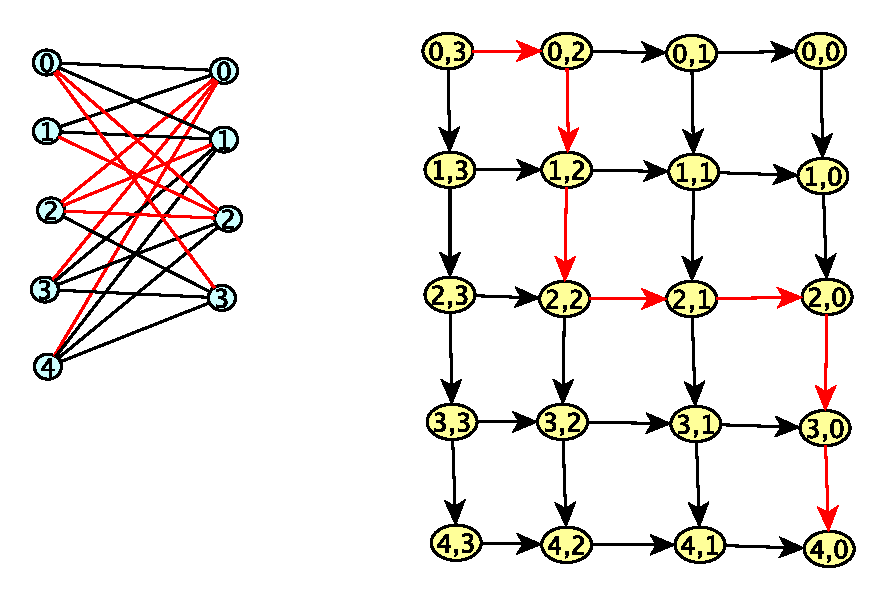
\includegraphics[height=7cm]{images_these/NonCrossingM.pdf}}
	\caption[Un chemin dans $H$ associé à un ensemble d'arêtes croisées dans G]{ Un chemin dans H associé à un ensemble d'arêtes croisées dans $G$.}
	\label{NonCrossingM}
\end{figure}

\begin{Lem}\label{lem_antcste}
	Pour tout plus long chemin $P$ dans $H$, la contrainte antagoniste engendrée par $P$ est valide pour $MILP_{SMEPC}$.
\end{Lem}
La démonstration de ce lemme se trouve en annexe à la section \ref{lem_antcste_section}.

\subsection{Polytope des correspondances non croisées}\label{NonCross}
Soit $Q$ le polytope défini par les contraintes (\ref{poly_me}).

\begin{subequations}\label{poly_me}
	\begin{align}
0 \leq U_{i,j} \leq 1,& \forall 0 \leq i \leq N-1, 0 \leq j \leq M &\label{positivite}\\
\sum_{(i, j) \in E(P)} U_{i,j} \leq 1,& \forall  P \in {\cal P}. &\label{antichaine}
\end{align}
\end{subequations}


{\it Une antichaine} $A$ de $(V(H),\preceq)$ est un sous-ensemble d'éléments de $V(H)$ incomparables par paires, c'est-à-dire que $A$ est l'ensemble de sommets de $V(H)$ de telle sorte que soit $(i_1,j_1)\npreceq (i_2,j_2)$ ou $(i_2,j_2)\npreceq (i_1,j_1)$ pour tout $(i_1,j_1)\in A, (i_2,j_2) \in A,(i_1,j_1)\neq (i_2,j_2)$.

Le polytope $Q$ est précisément le polytope de chaînes dont les sommets sont les vecteurs caractéristiques des antichaînes de $(V(H),\preceq)$.
%~(\cite{Sch}).

\begin{Lem}\label{lem_antichMatch}
	Une antichaine $A$ de $(V(H),\preceq)$ correspond à un ensemble de correspondance non croisée de $G$.
\end{Lem}
La démonstration de ce lemme se trouve en annexe à la section \ref{lem_antichMatch_section}.

D'après les lemmes (\ref{lem_antcste}) et (\ref{lem_antichMatch}), les sommets du polytope $Q$ sont des vecteurs caractéristiques des correspondances non croisés de $G$.

De plus, les contraintes antagonistes peuvent être utilisées pour renforcer la relaxation linéaire $RMILP_{SMEPC}$ de la section~\ref{sec4}.
Vérifier si une solution faisable $U$ de la relaxation linéaire satisfait des inégalités de type (\ref{clique_antag_P}) peut être effectué en temps polynomial
en cherchant le plus long chemin sur le digraphe acyclique $H$ avec l'algorithme de Bellman.

\subsection{Correspondance Time-consistent}

Cette section se concentre sur une sous-classe de correspondances non croisées.
Étant donné le graphe biparti complet $G=(I+J, E(G))$ et une fonction de poids $w : J \times J \rightarrow \mathbb{Z}_+$, nous disons que deux arêtes $(i,j)$ et $(i',j')$, avec $j <j'$, d'une correspondance dans $G$ sont \emph{ time-consistent} (respectivement \emph{ time-inconsistent}) si   $i+w(j,j') \leq i'$ (respectivement $i+w(j,j') > i'$). Un correspondance $C$ est dite {\it time-consistent} si $C$ est un sous-ensemble d'arêtes time-consistent par paires.

Notez que, comme $w(j, j') \geq 0, \textrm{ for all } 0 \leq j < j' \leq M$,  une correspondance time-consistent $C$ est aussi une correspondance non croisée de $G$. 
En effet, si deux arêtes $(i,j)$ et $(i',j')$ avec $j<j'$ appartiennent à $C$, alors nous avons $i' \geq i$, et les deux arêtes sont nécessairement non croisées.

Dans la tournée, le véhicule se déplace de la station $j$ vers une autre station $j'$ et ne peut pas atteindre $j'$ plus rapidement que le temps nécessaire pour le trajet en ligne droite entre $j$ et $j'$.
Les valeurs entières $w(j, j'), 0 \leq j < j' \leq M$, reflètent ce temps incompressible. 

\begin{Lem}\label{lem_ComplexIncons}
	Étant donné un graphe biparti complet $G=(I+J, E(G))$, une fonction de poids $w : J \times J \rightarrow \mathbb{Z}_+$ et un entier $k$, 
	le problème de la recherche d'une correspondance time-consistent de taille $k$ dans $G$ est $NP$-complet.
\end{Lem}
La démonstration de ce lemme se trouve en annexe à la section \ref{lem_ComplexIncons_section}.

Le lemme précédent suggère qu'une description complète du polytope des correspondances time-consistent est difficile à obtenir pour toute fonction de poids $w$. 
%%%%%%


\begin{figure}[H]
	\centerline{
		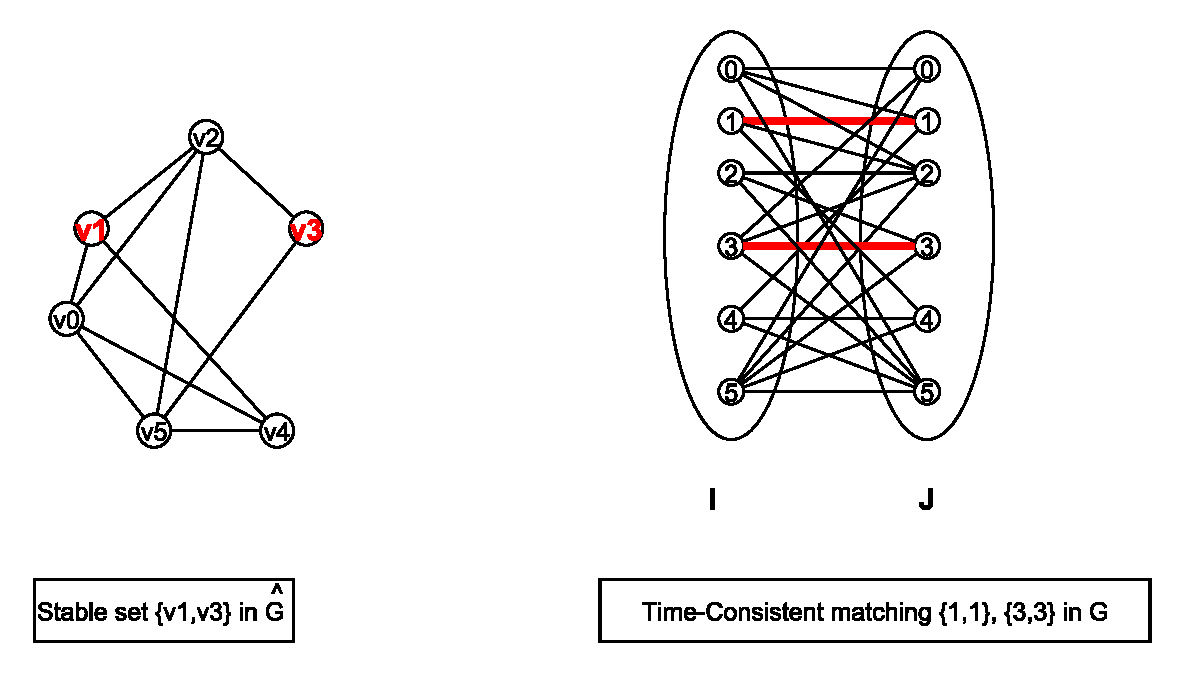
\includegraphics[height=7cm]{images_these/ConsistCompl.pdf}}
	\caption[Transformation d'un ensemble stable dans $H$ en un appariement conforme au temps dans G]{ Transformation d'un ensemble stable dans H en un croissement Time-consistent dans G.}
	\label{ConsistCompl}
\end{figure}

Dans la dernière partie de cette sous-section, nous supposons que la fonction de poids satisfait la propriété \emph{(SA)}.
$$ \begin{array}{lr}
\forall j_1, j_2, j_3 \in \llbracket 0, M \rrbracket, j_1 < j_2 < j_3 \Rightarrow w(j_1, j_2) + w(j_2, j_3) \leq w(j_1, j_3) & \textrm{(SA)}
\end{array} $$ 
%
Alors, si les paires $\{(i_1, j_1), (i_2, j_2) \}$ et  $\{(i_2, j_2), (i_3, j_3) \}$ sont time-inconsistent
pour certains $ 0\leq j_1 < j_2< j_3 \leq M$ et $ 0\leq i_1 < i_2 < i_3 \leq N-1$, alors 
la paire $\{(i_1, j_1), (i_3, j_3) \}$ est aussi time-inconsistent.

En ce qui concerne la propriété (SA), des contraintes valides peuvent être obtenues comme dans la section \ref{Non_crossing_matchings}.
Tout d'abord, complétons le graphe acyclique dirigé $H$ de la section \ref{Non_crossing_matchings} comme suit.
Pour tout $j < j'$ tel que $w(j, j') \geq 2$, nous ajoutons les arcs $((i' ,j'), (i,j))$ pour $ \max(0, i' - w(j, j') +1) \leq i \leq i'-1, 1 \leq i' \leq N-1$.
Désignons par $H_\textrm{tc}$ ce graphe modifié, par $A^+(H_\textrm{tc})$ l'ensemble des nouveaux arcs, et par ${\cal P}_\textrm{tc}$ l'ensemble des chemins $P$ qui commence à $(0, M)$ et se termine à $(N-1, 0)$ dans $H_\textrm{tc}$.

Ainsi, pour un plus long chemin $P \in {\cal P}_\textrm{tc}$, la contrainte (\ref{clique_timecons_P}) est appelé une contrainte {\it time-consistent} associée à $P$. 
\begin{eqnarray}
\sum_{(i, j) \in E(P)} U_{i,j} \le 1 &\label{clique_timecons_P}
\end{eqnarray}

\begin{Lem}\label{lem_arc_time}
	Soit $(i_0', j_0') $  et $(i_0, j_0) $ deux sommets de $H_\textrm{tc}$ tel que	$i_0' > i_0 $ et $j_0' > j_0 $. S'il existe un chemin dans $H_\textrm{tc}$ de $(i_0', j_0') $ à $(i_0, j_0) $, alors l'arc $((i_0', j_0'), (i_0, j_0)) $ existe dans $A^+(H_\textrm{tc})$.
\end{Lem}
La démonstration de ce lemme se trouve en annexe à la section \ref{dem_PTASlem_arc_time_section}.

\begin{Lem}\label{lem_timecons}
	Pour tout plus long chemin $P$ dans $H_\textrm{tc}$, la contrainte time-consistent induit par $P$ est valide pour $MILP_{SMEPC}$.
\end{Lem}
La démonstration de ce lemme se trouve en annexe à la section \ref{lem_timecons_section}.

De la même façon qu'à la section \ref{NonCross}, on peut voir que le polytope $Q_{t_c}$, défini par les inégalités (\ref{positivite}) et (\ref{clique_timecons_P}), pour tout chemin $P \in {\cal P}_\textrm{tc}$,
décrit la surface convexe des vecteurs qui caractérisent des correspondances time-consistent, lorsque la propriété $(SA)$ est satisfaite.

Pour $0\leq j<j'\leq M$, soit $\tilde{w}(j, j')=\sum_{k=j+1}^{j'-1} t_k, j'>j+1$ et $0$ sinon. 
il est évident que les valeurs $\tilde{w}(j,j')$ satisfont la propriété $(SA)$ et permettent une génération de contraintes time-consistent.
% ce qui est testé dans la partie expérimentale.


}
\section{Complexité du modèle SMEPC}
\label{NP-hard_SMEPC}
Dans cette partie,nous montrons que, même lorsque le coût fixe de production $Cost^F$ est nul, le \textbf{SMEPC} se réduit au problème du sac à dos. Cela nous permet d'établir le théorème \ref{smepc_difficilee}. 
\begin{theo}\label{smepc_difficilee}
SMEPC est NP-difficile.
\end{theo}
%\subsection{Généralités sur la complexité}
%définir les termes de compléxité
%\subsection{Démonstration : SMEPC est NP-difficile}
La démonstration de ce théorème se trouve en annexe à la section \ref{smepc_difficilee_section}.

 Après la présentation des résultats des expérimentations, nous nous attaquerons à la résolution proprement dites du problème à l'aide d'un schéma de programmation dynamique.  


\section{Expérimentations numériques}
\label{num_MIP}
\subsection{Objectifs et contexte technique}
L'objectif des expérimentations est de tester les formulations linéaires que nous avons proposé. Les modèles ont été implémentés en C++ et l'IDE utilisé est Visual Studio 2017.
Les expérimentations sont réalisées sur un ordinateur équipé d'un processeur AMD EPYC 7H12 64-Core, 512 Go de RAM et
fonctionnent sous Gnu/linux Ubuntu 20.04.2. Une première série d'expérimentations est réalisée au cours de laquelle CPLEX 12.10 est utilisé en mode 8 \textit{threads} 
%avec tous ses paramètres réglés sur leurs valeurs par défaut 
et le temps maximum du CPU est fixé à 3 heures. Les bornes supérieures obtenues seront utilisées comme valeurs de référence pour calculer les gaps tout au long de ce document. Une deuxième série d'expérimentations est réalisée au cours de laquelle CPLEX 12.10 est utilisé en mode \textit{single-threads} et le temps maximum du CPU est fixé à 1 heure.% avec tous ses paramètres réglés sur leurs valeurs par défaut 

\subsection{Procédés de génération d'instances du SMEPC}
\label{Gen_instance}
Pour faire des expérimentations, on a besoin d'instances du problème SMEPC. Étant donné que ce dernier est un nouveau problème, on a dû concevoir des procédés de génération de ses instances. On a un ensemble de 50 instances qui se subdivisent en deux paquets d'instances (paquet INST\_CTE et paquet INST\_VAR) car elles sont générées avec deux procédés différents. On a fixé que toutes nos entrées soient des valeurs entiers donc toutes nos variables le seront aussi. Dans cette section, on décrit les deux procédés de génération. 

Le paquet d'instances INST\_VAR a été généré avec une loi uniforme c'est pour cette raison que ces instances se \og ressemblent \fg{}. 
Pour pouvoir tester les performances de nos modèles on avait besoin d'instances suffisamment \og variées \fg{}, on a donc généré les instances du paquet INST\_CTE.
La génération d'instances ici consiste à générer le nombre de stations, les cordonnées de ces stations, les cordonnées du dépôt et les cordonnées de la micro-usine, le temps maximal, la durée d'une période, les rendements de production, les couts variables , les couts fixes de production, les quantités d'hydrogènes initiales dans le véhicule et dans la citerne et les capacités du véhicule et de la citerne.

Certaines étapes de la génération sont communes aux deux méthodes à l'instar de :
\begin{itemize}[label=$\square$]
	\item$xrectangle$, $yrectangle$ : Limite des coordonnées des stations respectivement sur l'axe des abscisses et l'axe des ordonnées. On considère que deux stations ne peuvent pas avoir les mêmes coordonnées. On fixe le rectangle dans lequel on place les stations aléatoirement, une station est un point dans le plan. Les valeurs entières $xrectangle$ et $yrectangle$ représentent respectivement la longueur en abscisse et en ordonné de ce rectangle (Voir figure \ref{Fr_gen_station}). Avec par exemple $(xrectangle,yrectangle) \in [1, M]^2 $. 
	\begin{figure}[H]
		\centerline{
			\includegraphics[height=8cm]{images_these/gen_station.pdf}}
		\caption[Plan contenant les stations]{Plan contenant les stations.}
		\label{Fr_gen_station}
	\end{figure}
	Si le dépôt a pour coordonnées $(a,b)$ alors la micro-usine aura pour coordonnées $(a,b+1)$ car on impose qu'il y ait une distance de 1 unité entre le dépôt et la micro-usine.
	
	%Nous fixons aléatoirement les stations comme des points dans un rectangle de dimension $xrectangle \times yrectangle$ , où deux stations ne peuvent pas avoir les mêmes coordonnées. Lamicro-usine sera proche du dépôt. Les coordonnées de la micro-usine sont $(x,y+1)$.
	\item A partir de ces coordonnées, la matrice des valeurs de distances est calculée comme la valeur arrondie de la distance euclidienne
	entre deux stations, et la matrice des valeurs d'énergie comme la valeur de la distance de Manhattan.
	Autrement dit, les valeurs de distances $d_j$, $d^*_j$, $t_j$ et les valeurs d'énergies $e_j$, $\varepsilon_j$, $\varepsilon^*_j$ correspondent respectivement à l'arrondi (partie entière supérieure) de la distance euclidienne et à la distance de Manhattan.
\end{itemize}
\subsubsection{Génération du paquet d'instances INST\_VAR}
On génère 30 instances avec le procédé de génération décrit par la suite.
 Nous fixons $M$ et $p$, et générons aléatoirement les stations $j$ et la station particulière $Depot$ comme point de l'espace $\mathbb{R}^2$.  
 On génère des instances aléatoirement de la façon suivante :

\begin{enumerate}
	\item On fixe aléatoirement $M$ le nombre de stations ($M>2$). Car on doit avoir au moins deux stations pour réaliser les tâches de transport et de livraison.
	\item On fixe aléatoirement $p$ la taille d'une période.
	\item On fixe le paramètre de la fonction objectif $\alpha=1$.% et $\beta=1$. 
	%\item On fixe le rectangle dans lequel on place les stations aléatoirement, une station est un point dans le plan. Les valeurs entières $xrectangle$ et $yrectangle$ représentent respectivement la longueur en abscisse et en ordonné de ce rectangle (Voir figure \ref{Fr_gen_station}). Avec par exemple $(xrectangle,yrectangle) \in [1, M]^2 $. 
%	\begin{figure}[H]
	%	\centerline{
	%		\includegraphics[height=8cm]{images_these/gen_station.pdf}}
	%	\caption[Plan contenant les stations]{Plan contenant les stations.}
	%	\label{Fr_gen_station}
	%\end{figure}
	%Si le dépôt a pour coordonné $(a,b)$ alors la micro-usine aura pour coordonnée $(a,b+1)$ car on impose qu'il y ait une distance de 1 unité entre le dépôt et la micro-usine.
	\item On fixe $E_0$, par exemple $E_0 \in [1, M]$. $E_0$ doit au moins être égale à 1 car il faut pouvoir se rendre à la micro-usine à partir du dépôt initial.
	\item On fixe le paramètre entier $param\_vmax$, par exemple $param\_vmax \in [2,3]$. On calcule $C^{Veh}$ tel que $C^{Veh}= \frac{\sum_{j \leq M} e_j }{ param\_vmax} +E_0$. L'idée ici est d'imposer qu'il faut au moins $param\_vmax$ recharges pour pouvoir finir la tournée.
	\item On fixe le paramètre entier $param\_cit \in [1,3]$. On calcule $C^{Tank}$ tel que $C^{Tank}=param\_cit \times C^{Veh}$. L'idée ici est d'imposer que si la citerne est pleine on peut remplir au plus $param\_cit$ fois le réservoir du véhicule sans production. 
	
	\item On fixe $Cost^F$, par exemple $Cost^F \in [1, 3\times M]$.  
	\item On fixe $H_0$, par exemple $H_0 \in [0, M]$. %On évite que $H_0$ soit très grand pour être certain qu'il y aura production.
	\item On fixe le paramètre entier $param\_tmax$, par exemple $param\_tmax\in [2,3]$. On calcule $TMax$ tel que $TMax \geq \sum_{j \leq M} d_j \times param\_tmax$. On fixe $TMax$ ainsi pour être sûr d'avoir suffisamment de temps pour finir la tournée.
	\item On calcule $N=\lceil \frac{TMax}{p}\rceil$.% en s'assurant que $N$ soit une valeur entière en prenant la partie entière supérieure.
	\item On fixe le paramètre entier $xrendement$, par exemple $xrendement \in [2,3]$. Le rendement de production de chaque période est fixé aléatoirement dans l'intervalle $[1, \frac{C^{Tank}}{xrendement}]$. L'idée ici est d'imposer qu'il faudrait au moins produire sur deux périodes pour pouvoir remplir la citerne.
	\item On fixe le paramètre entier $xcout$, par exemple $xcout \in [1, M]$. Le coût de production de chaque période est fixé aléatoirement dans l'intervalle $[1, xcout]$.
\end{enumerate}

%Pour contrôler la taille des instances, on s'assure que le nombre d'états générés maximal ne dépasse pas un certains seuil noté $SEUIL\_STATE$ (Avec la formule $C^{Veh}\times C^{Tank} \times  M\times N \times 2 \leq SEUIL\_STATE$).

%Ensuite, nous fixons $C^{Tank}$, $C^{Veh}$ et $TMax$, de telle sorte que cela assure l'existence d'une solution réalisable. Enfin, nous fixons les coefficients de coût, de telle sorte que le coût fixe $Cost^F$ soit au moins égal au plus grand coefficient $Cost^V_i$, $i = 0, \dots, N - 1$. 

%Dans le cas présent, nous utilisons un ensemble de 30 instances, avec les caractéristiques $N$, $M$, $TMax$, $p$, $C^{Veh}$, $C^{Tank}$ présenté par le tableau (\ref{tab:inst}). La signification de ces caractéristiques est :

%\begin{itemize}[label=$\square$]
%	\item $N$ : Nombre de périodes de production ; 
%	\item $M$ : Nombre de stations (Dépôt et micro-usine exclus) ; 
%	\item $TMax$ : Le délai maximal pour que le véhicule puisse effectuer sa tournée ;
%	\item $p$ : Durée en unités de temps d'une période de production ;
%	\item $C^{Veh}$ : Capacité du réservoir d'hydrogène du véhicule ; 
%	\item $C^{Tank}$ : Capacité de la citerne d'hydrogène.
%\end{itemize}

\subsubsection{Génération du paquet d'instances INST\_CTE}
On génère 20 instances avec le procédé de génération décrit par la suite. Avant de le décrire on présente les paramètres du processus de génération :
\begin{itemize}[label=$\square$]
	%\item $N$ : Nombre de périodes ;
	%\item $M$ : Nombre de stations, sans compter le Dépôt et la micro-usine ;
	%\item $xrectangle$, $yrectangle$ : Limite des coordonnées des stations respectivement sur l'axe des abscisses et l'axe des ordonnés ;
	\item $K $ : Le nombre d'intervalles, ainsi les N périodes seront divisées en $K$ intervalles. Pour des raisons de
	simplicité, nous allons faire en sorte que ces intervalles aient le même nombre de périodes. Nous ajoutons le paramètre $n$, qui sera le nombre de périodes d'un intervalle.
	Pour ce motif, $N$ ne sera pas un paramètre et il sera calculé comme $N= n\times K$.
	\item $Q$ exprime la contrainte induite par les besoins énergétiques (énergie à recharger) du véhicule et la capacité de stockage du véhicule, il s'agit du
	nombre de recharges prévu.
	\item $H$ : Le rapport entre la capacité de la citerne et le réservoir du véhicule.
	\item $R$ exprime la contrainte induite par les besoins énergétiques du véhicule sur l'activité de production.
	\item $S$ : Le rapport entre la part du coût due à la consommation d'énergie et la part
	du coût due à l'activation de la micro-usine.
	%\item $\alpha$ : Le taux de conversion qui permet de transformer le temps en valeur de coût. Ce paramètre seracalculé en multipliant un coefficient Cα par le coût unitaire moyen.
	
\end{itemize}


Nous calculons l'énergie minimale attendue $E^*$ comme l'énergie nécessaire dans une tournée simple construite de la
manière suivante : en partant du dépôt, nous sélectionnons itérativement la station non visitée la plus proche jusqu'à ce que toutes les stations soient visitées, puis, nous retournons au dépôt final. Nous calculons également l'énergie moyenne pour
se rendre à la micro-usine $E_{mean}^{MP}=\frac{1}{M+1}\sum_{ 0 \leq i \leq M}\varepsilon_i$.

Pour chaque intervalle $k \in K$, nous générons aléatoirement 2 nombres $\Pi_k$ avec $k \in 1, \dots, 5$ et $\Theta_k$ avec $k \in 1, \dots, 3$.
Pour chaque période $i$ de l'intervalle $k$, nous générons aléatoirement un taux de production $RAux_i$
et un coût de production variable $Cost^V_i$
selon la distribution uniforme respectivement à l'intérieur des intervalles $[\Pi_k/2, 3\Pi_k/2]$ et $[\Theta_k/2, 3\Theta_k/2]$.
Ensuite, nous obtenons le coût de production $R_i = \lambda\times RAux_i$,
en choisissant $\lambda$ de telle sorte que $\sum_i R_i=R\times E^*$. Nous calculons le coût moyen unitaire : $C_{mean}=(\sum_i Cost_i^V/R_i)\times N$. 

Nous fixons $C^{Veh} = E^*/Q + E^{MP}_{mean}$, nous ajoutons $E^{MP}_{mean}$ pour prendre en compte le fait que le véhicule
a également besoin de capacité pour aller se ravitailler en carburant et pour les bonnes tournées, le nombre de recharges est
approximativement $Q$. Nous fixons $C^{Tank} = H \times C^{Veh}$ et nous fixons le coût de production fixe : $Cost^F=\frac{C_{mean}\times E^*}{2S\times (1+E^*/C^{Veh})}$.

\subsection{Caractéristiques des instances}
Toutes les séries d'expériences concernent les instances présentées dans les tableaux (\ref{tab:inst}) et (\ref{tab:inst2}) avec les notations suivantes :

\begin{itemize}[label=$\square$]
	\item $num$ : Numéro de l'instance ;
	\item $M$ : Nombre de stations ;
	\item $N$ : Nombre de périodes ;
	\item $p$ : Durée d'une période ;
	\item $H_0$ : Quantité d'hydrogène initiale dans la citerne ;
	\item $C^{Tank}$ : Capacité maximale de la citerne ;
	\item $E_0$ : Quantité d'hydrogène initiale dans le réservoir du véhicule ;
	\item $C^{Veh}$ : Capacité maximale du réservoir ;
	\item $LTour$ : Durée de la tournée sans recharge ;
	\item $ETour$ : Énergie de la tournée sans recharge.
\end{itemize}
Les tableaux (\ref{tab:inst}) et (\ref{tab:inst2}) représentent respectivement les caractéristiques du paquet d'instances INST\_VAR et celles du paquet d'instances INST\_CTE.
On fait les remarques suivantes :
\begin{itemize}[label=$\square$]
	\item  Pour la plupart des instances du paquet INST\_VAR, l'énergie initial $E_0$ du véhicule est très petite par rapport à l'énergie de la tournée sans recharge $ETour$. Or cela n'est pas le cas pour les instances du paquet INST\_CTE ;
	\item Pour la plupart des instances du paquet INST\_VAR, l'énergie initial $E_0$ du véhicule est très petite par rapport à la capacité du véhicule $C^{Veh}$. Or cela n'est pas le cas pour les instances du paquet INST\_CTE ; on fait la même remarque pour $H_0$ par rapport à $C^{Tank}$ ;
	\item Les capacités du véhicule et de la citerne du paquet d'instances INST\_VAR sont très élevées par rapport à celles du paquet d'instances INST\_CTE ;
	\item Le nombre de périodes $N$ des instances du paquet INST\_CTE est constant, or, dans le paquet d'instances INST\_VAR on a différentes valeurs de $N$ ;
	\item Pour la plupart des instances, les valeurs de $N$ du paquet d'instances INST\_VAR sont très élevées par rapport à celles du paquet d'instances INST\_CTE ;
	\item Pour la plupart des instances, les valeurs de $p$ du paquet d'instances INST\_VAR sont très faibles par rapport à celles du paquet d'instances INST\_CTE.
\end{itemize}

\subsubsection{Caractéristiques des instances du paquet INST\_VAR}
%%%%%%Ar  DAM
Le tableau (\ref{tab:inst}) présente les caractéristiques des instances du paquet INST\_VAR.
Le paquet d'instances INST\_VAR est constitué de 30 instances. On a des instances de 8, 10, 12, 15, 20, 30, 50, 70 et 100 stations. La durée d'une période vaut 1, 2, 4, 5, 6, 8 et 10.
\begin{table}[H]
	\centering
	\small{
		\begin{tabular}{|r|r|r|r|r|r|r|r|r|r|}
			\hline
			\toprule
			\rowcolor{cyan}	\textbf{num} &$\mathbf{M}$ & $\mathbf{N}$ & $\mathbf{p}$ &  $\mathbf{H_0} $ & $\mathbf{C^{Tank}}$ & $\mathbf{E_0}$ & $\mathbf{C^{Veh}}$ & \textbf{LTour} & \textbf{Etour} \\
			\midrule
			\hline
			1	&	8	&	20	&	4	&	6	&	25	&	8	&	12	&	20	&	20	\\ \hline
			2	&	8	&	25	&	4	&	5	&	20	&	8	&	10	&	25	&	26	\\ \hline
			3	&	8	&	40	&	5	&	10	&	70	&	20	&	30	&	44	&	50	\\ \hline
			4	&	10	&	36	&	2	&	8	&	25	&	9	&	12	&	36	&	38	\\ \hline
			5	&	10	&	50	&	4	&	6	&	40	&	10	&	20	&	50	&	54	\\ \hline
			6	&	10	&	94	&	1	&	3	&	30	&	4	&	15	&	47	&	52	\\ \hline
			7	&	12	&	32	&	4	&	0	&	50	&	4	&	25	&	63	&	68	\\ \hline
			8	&	12	&	50	&	4	&	3	&	36	&	3	&	18	&	50	&	58	\\ \hline
			9	&	15	&	160	&	4	&	8	&	240	&	20	&	120	&	426	&	556	\\ \hline
			10	&	20	&	108	&	10	&	20	&	390	&	10	&	190	&	716	&	894	\\ \hline
			11	&	10	&	80	&	2	&	10	&	40	&	10	&	20	&	38	&	38	\\ \hline
			12	&	15	&	327	&	4	&	20	&	400	&	11	&	140	&	653	&	790	\\ \hline
			13	&	20	&	180	&	6	&	3	&	500	&	20	&	170	&	718	&	834	\\ \hline
			14	&	20	&	440	&	5	&	100	&	350	&	50	&	170	&	910	&	1164	\\ \hline
			15	&	30	&	177	&	8	&	6	&	420	&	10	&	200	&	944	&	1188	\\ \hline
			16	&	30	&	260	&	6	&	50	&	400	&	50	&	200	&	1034	&	1320	\\ \hline
			17	&	30	&	544	&	4	&	10	&	560	&	15	&	250	&	1088	&	1382	\\ \hline
			18	&	50	&	265	&	10	&	6	&	400	&	9	&	200	&	1764	&	2216	\\ \hline
			19	&	50	&	500	&	8	&	100	&	420	&	50	&	180	&	1565	&	2000	\\ \hline
			20	&	70	&	328	&	10	&	15	&	550	&	25	&	270	&	2183	&	2766	\\ \hline
			21	&	30	&	1100	&	2	&	100	&	400	&	80	&	200	&	1097	&	1342	\\ \hline
			22	&	30	&	1200	&	2	&	100	&	400	&	70	&	200	&	957	&	1200	\\ \hline
			23	&	50	&	634	&	6	&	50	&	300	&	50	&	150	&	1542	&	1938	\\ \hline
			24	&	50	&	850	&	4	&	20	&	400	&	50	&	180	&	1941	&	2500	\\ \hline
			25	&	50	&	1125	&	4	&	20	&	700	&	50	&	280	&	1718	&	2128	\\ \hline
			26	&	70	&	383	&	8	&	20	&	760	&	15	&	240	&	2039	&	2590	\\ \hline
			27	&	70	&	683	&	8	&	8	&	850	&	14	&	370	&	2185	&	2826	\\ \hline
			28	&	70	&	984	&	6	&	50	&	750	&	40	&	250	&	2340	&	2926	\\ \hline
			29	&	100	&	651	&	8	&	100	&	600	&	60	&	200	&	3471	&	4360	\\ \hline
			30	&	100	&	800	&	10	&	100	&	950	&	100	&	430	&	3095	&	3796	\\ \hline
			
			\bottomrule
		\end{tabular}%
	}\caption{Caractéristiques des instances du paquet INST\_VAR}
	\label{tab:inst}%
\end{table}%
\subsubsection{Caractéristiques des instances du paquet INST\_CTE}
Le tableau (\ref{tab:inst2}) présente les caractéristiques des instances du paquet INST\_CTE.
Le paquet d'instances INST\_CTE est constitué de 20 instances. On a des instances de 10, 20, 30, 50, 75 et 100 stations. Le nombre de périodes est fixe. Le nombre de périodes est 20 pour toutes les instances. La durée d'une période vaut 5, 10, 14, 34, 58 et 65.  
\begin{table}[H]
	\centering
	\small{
		\begin{tabular}{|r|r|r|r|r|r|r|r|r|r|}
			\hline
			\toprule
			\rowcolor{cyan}	\textbf{num} &$\mathbf{M}$ & $\mathbf{N}$ & $\mathbf{p}$ &  $\mathbf{H_0} $ & $\mathbf{C^{Tank}}$ & $\mathbf{E_0}$ & $\mathbf{C^{Veh}}$ & \textbf{LTour} & \textbf{Etour} \\
			\midrule
			\hline
			31	&	10	&	20	&	5	&	51	&	73	&	34	&	49	&	48	&	54	\\ \hline
			32	&	10	&	20	&	5	&	48	&	69	&	32	&	46	&	50	&	56	\\ \hline
			33	&	10	&	20	&	5	&	42	&	60	&	28	&	40	&	47	&	54	\\ \hline
			34	&	10	&	20	&	5	&	54	&	78	&	36	&	52	&	46	&	52	\\ \hline
			35	&	20	&	20	&	10	&	65	&	94	&	32	&	47	&	84	&	100	\\ \hline
			36	&	20	&	20	&	10	&	72	&	104	&	36	&	52	&	73	&	78	\\ \hline
			37	&	20	&	20	&	10	&	42	&	60	&	42	&	60	&	78	&	82	\\ \hline
			38	&	20	&	20	&	10	&	35	&	51	&	35	&	51	&	101	&	112	\\ \hline
			39	&	20	&	20	&	10	&	34	&	49	&	34	&	49	&	73	&	80	\\ \hline
			40	&	30	&	20	&	14	&	85	&	122	&	85	&	122	&	136	&	156	\\ \hline
			41	&	50	&	20	&	34	&	65	&	93	&	43	&	62	&	218	&	238	\\ \hline
			42	&	50	&	20	&	34	&	56	&	81	&	37	&	54	&	205	&	224	\\ \hline
			43	&	75	&	20	&	58	&	102	&	147	&	41	&	59	&	275	&	308	\\ \hline
			44	&	75	&	20	&	58	&	109	&	157	&	44	&	63	&	217	&	232	\\ \hline
			45	&	100	&	20	&	65	&	198	&	284	&	49	&	71	&	265	&	278	\\ \hline
			46	&	100	&	20	&	65	&	232	&	332	&	58	&	83	&	283	&	298	\\ \hline
			47	&	100	&	20	&	65	&	233	&	333	&	77	&	111	&	274	&	284	\\ \hline
			48	&	100	&	20	&	65	&	256	&	366	&	85	&	122	&	386	&	424	\\ \hline
			49	&	100	&	20	&	65	&	203	&	291	&	67	&	97	&	253	&	260	\\ \hline
			50	&	100	&	20	&	65	&	165	&	237	&	55	&	79	&	256	&	268	\\ \hline
			
			\bottomrule
		\end{tabular}%
	}\caption{Caractéristiques des instances du paquet INST\_CTE}
	\label{tab:inst2}%
\end{table}%


\subsection{Caractéristiques des solutions}
Dans cette section, on présente les caractéristiques des solutions des 50 instances générées. Ces solutions ont été obtenues par le modèle $MILP_{SMEPC}$ en y ajoutant les contraintes (STC), (EC1), (EC2) et (EC3). Lorsque la solution optimale n'est pas connue, on donne les caractéristiques de la borne supérieure. La liste de ces caractéristiques est :
\begin{itemize}[label=$\square$]
	\item $\mathbf{nbRech}$ : Nombre de recharges ;
	\item $\mathbf{nbSetup}$ : Nombre d'activations de la micro-usine
	\item $\mathbf{prod}$ : Hydrogène produite pour réaliser la tournée ;
	\item  $\mathbf{conso} $ :  Hydrogène consommée par le véhicule pour réaliser la tournée ;
	\item $\mathbf{wait time}$ : Temps d'attente du véhicule ;
	\item $\mathbf{cost time}$ : Coût en temps de la solution ;
	 \item $\mathbf{cost prod}$ : Coût de production de la solution.
\end{itemize}

En moyenne, on constate que pour toutes les instances, la durée de la tournée $\mathbf{cost time}$ est très élevée par rapport à la durée de la tournée sans recharge  $LTour$, ce qui peut vouloir dire que le véhicule attend \og beaucoup \fg{} avant de se recharger ou que la durée des détours est très élevée. On remarque aussi qu'il n'y a pas un grand gap entre la quantité d'hydrogène produite et la quantité d'hydrogène consommée, ce qui peut vouloir dire qu'on ne produit pas de façon excessive.

Les tableaux (\ref{tab:sol}) et (\ref{tab:sol2}) représentent respectivement les caractéristiques des solutions du paquet d'instances INST\_VAR et celles du paquet d'instances INST\_CTE.
On fait les remarques suivantes :
\begin{itemize}[label=$\square$]
	\item Concernant les instances du paquet INST\_VAR, le temps d'attente $wait time$ du véhicule est très faible par rapport au coût en temps $cost time$ du processus, on passe en moyenne 58,62\% du temps à attendre. Or cela n'est pas la cas pour les instances du paquet INST\_CTE ;
	\item Globalement, le nombre de recharge du paquet d'instances INST\_VAR est supérieur au nombre de recharge du paquet d'instances INST\_CTE, cela est peut-être dû au fait que les valeurs $E_0$ du paquet INST\_VAR sont très petites par rapport aux valeurs $Etour$ ;
	\item  Concernant les instances du paquet INST\_VAR, le coût de production $cost prod$ est très faible par rapport au coût en temps $cost time$. Or cela n'est pas le cas pour les instances du paquet INST\_CTE. 
	\item La quantité d'hydrogène produite et consommée du paquet d'instances INST\_VAR est très élevée par rapport à celle du paquet d'instances INST\_CTE ; 
\end{itemize}
\subsubsection{Caractéristiques des solutions des instances du paquet INST\_VAR}
Le tableau (\ref{tab:sol}) présente les caractéristiques des solutions des instances du paquet INST\_VAR. 

 %Les instances 24, 25, 29 et 30 sont celles dont on n'a pas pu obtenir les solutions en moins d'une heure, on les a laissé s'exécuter durant plus longtemps. Pour avoir une borne supérieure, on a dû mettre le temps limite à 3 heures en utilisant 8 threads. %Pour obtenir les solutions de ces quatre instances on a supprimé du modèle $MILP_{SMEPC}$ les contraintes symétriques (\ref{39}).

 % En moyenne, la durée de la tournée $\mathbf{cost time}$ est très élevée par rapport à la durée de la tournée sans recharge  $LTour$, ce qui peut vouloir dire que le véhicule attend \og beaucoup \fg{} avant de se recharger ou que la durée des détours est très élevée. On remarque aussi qu'il n'y a pas un grand gap entre la quantité d'hydrogène produite et la quantité d'hydrogène consommée, ce qui peut vouloir dire qu'on ne produit pas de façon excessive.

\begin{table}[H]
	\centering
	\small{
		\begin{tabular}{|r|r|r|r|r|r|r|r|}
			\hline
			\toprule
			\rowcolor{cyan}	\textbf{num} &$\mathbf{nbRech}$ & $\mathbf{nbSetup}$ & $\mathbf{prod}$ &  $\mathbf{conso} $ & $\mathbf{wait time}$ & $\mathbf{cost time}$ & $\mathbf{cost prod}$  \\
			\midrule
			\hline
			1	&	3	&	2	&	29	&	28	&	30	&	57	&	74	\\ \hline
			2	&	5	&	2	&	34	&	34	&	40	&	73	&	78	\\ \hline
			3	&	3	&	2	&	64	&	62	&	25	&	81	&	63	\\ \hline
			4	&	5	&	2	&	42	&	42	&	26	&	67	&	73	\\ \hline
			5	&	5	&	2	&	63	&	60	&	29	&	85	&	76	\\ \hline
			6	&	7	&	4	&	72	&	72	&	8	&	73	&	105	\\ \hline
			7	&	5	&	3	&	92	&	90	&	39	&	121	&	101	\\ \hline
			8	&	6	&	2	&	69	&	66	&	58	&	121	&	71	\\ \hline
			9	&	7	&	4	&	624	&	622	&	40	&	509	&	135	\\ \hline
			10	&	8	&	4	&	1104	&	1084	&	133	&	1001	&	138	\\ \hline
			11	&	4	&	2	&	61	&	58	&	17	&	75	&	59	\\ \hline
			12	&	10	&	3	&	952	&	946	&	67	&	819	&	93	\\ \hline
			13	&	7	&	3	&	975	&	972	&	70	&	867	&	89	\\ \hline
			14	&	12	&	5	&	1442	&	1412	&	89	&	1231	&	141	\\ \hline
			15	&	8	&	5	&	1354	&	1328	&	107	&	1196	&	150	\\ \hline
			16	&	9	&	4	&	1391	&	1390	&	76	&	1160	&	131	\\ \hline
			17	&	8	&	3	&	1474	&	1424	&	50	&	1182	&	103	\\ \hline
			18	&	15	&	8	&	2400	&	2400	&	215	&	2125	&	248	\\ \hline
			19	&	17	&	6	&	2211	&	2210	&	187	&	1977	&	236	\\ \hline
			20	&	13	&	7	&	2851	&	2848	&	207	&	2449	&	210	\\ \hline
			21	&	11	&	5	&	1545	&	1488	&	28	&	1279	&	131	\\ \hline
			22	&	11	&	4	&	1500	&	1456	&	27	&	1221	&	121	\\ \hline
			23	&	22	&	11	&	2510	&	2510	&	178	&	2276	&	314	\\ \hline
			24	&	22	&	11	&	3036	&	3022	&	111	&	2517	&	288	\\ \hline
			25	&	12	&	5	&	2293	&	2278	&	65	&	1924	&	129	\\ \hline
			26	&	15	&	5	&	2617	&	2610	&	155	&	2244	&	112	\\ \hline
			27	&	11	&	5	&	2833	&	2828	&	113	&	2317	&	151	\\ \hline
			28	&	18	&	6	&	3374	&	3360	&	164	&	2879	&	175	\\ \hline
			29	&	30	&	10	&	4626	&	4616	&	411	&	4129	&	308	\\ \hline
			30	&	12	&	6	&	3871	&	3864	&	196	&	3362	&	160	\\ \hline
			
			
			\bottomrule
		\end{tabular}%
	}\caption{Caractéristiques des solutions des instances du paquet INST\_VAR}
	\label{tab:sol}%
\end{table}%
\subsubsection{Caractéristiques des solutions des instances du paquet INST\_CTE}
Le tableau (\ref{tab:sol2}) présente les caractéristiques des solutions des instances du paquet INST\_CTE. %En moyenne, on constate que la durée de la tournée $\mathbf{cost time}$ est très élevée par rapport à la durée de la tournée sans recharge  $LTour$, ce qui peut vouloir dire que le véhicule attend \og beaucoup \fg{} avant de se recharger ou que la durée des détours est très élevée. On remarque aussi qu'il n'y a pas un grand gap entre la quantité d'hydrogène produite et la quantité d'hydrogène consommée, ce qui peut vouloir dire qu'on ne produit pas de façon excessive.
\begin{table}[H]
	\centering
	\small{
		\begin{tabular}{|r|r|r|r|r|r|r|r|}
			\hline
			\toprule
			\rowcolor{cyan}	\textbf{num} &$\mathbf{nbRech}$ & $\mathbf{nbSetup}$ & $\mathbf{prod}$ &  $\mathbf{conso} $ & $\mathbf{wait time}$ & $\mathbf{cost time}$ & $\mathbf{cost prod}$  \\
			\midrule
			\hline
			31	&	2	&	2	&	59	&	56	&	16	&	66	&	175	\\ \hline
			32	&	3	&	2	&	64	&	64	&	23	&	81	&	277	\\ \hline
			33	&	2	&	2	&	56	&	56	&	11	&	61	&	162	\\ \hline
			34	&	2	&	2	&	54	&	54	&	11	&	61	&	141	\\ \hline
			35	&	4	&	2	&	121	&	114	&	53	&	151	&	106	\\ \hline
			36	&	3	&	1	&	98	&	92	&	57	&	141	&	85	\\ \hline
			37	&	2	&	2	&	87	&	84	&	32	&	111	&	66	\\ \hline
			38	&	4	&	4	&	122	&	120	&	62	&	171	&	111	\\ \hline
			39	&	4	&	4	&	118	&	114	&	47	&	151	&	162	\\ \hline
			40	&	2	&	4	&	169	&	160	&	38	&	177	&	159	\\ \hline
			41	&	6	&	6	&	290	&	290	&	355	&	613	&	288	\\ \hline
			42	&	7	&	6	&	283	&	280	&	363	&	613	&	827	\\ \hline
			43	&	9	&	8	&	464	&	402	&	743	&	1103	&	433	\\ \hline
			44	&	6	&	3	&	294	&	294	&	485	&	755	&	164	\\ \hline
			45	&	6	&	6	&	385	&	380	&	453	&	794	&	135	\\ \hline
			46	&	5	&	3	&	338	&	338	&	466	&	781	&	70	\\ \hline
			47	&	4	&	3	&	409	&	358	&	379	&	716	&	226	\\ \hline
			48	&	5	&	3	&	517	&	502	&	598	&	1041	&	209	\\ \hline
			49	&	4	&	3	&	340	&	340	&	394	&	716	&	115	\\ \hline
			50	&	6	&	6	&	385	&	372	&	503	&	846	&	234	\\ \hline
			
			
			
			\bottomrule
		\end{tabular}%
	}\caption{Caractéristiques des solutions des instances du paquet INST\_CTE}
	\label{tab:sol2}%
\end{table}%

\subsection{Résultats du modèle $MILP_{SMEPC}$ avec temps limite de 3 heures et 8 \textit{threads}}
Cette section présente les résultats du modèle $MILP_{SMEPC}$ avec les contraintes (STC), (EC1), (EC2) et (EC3) . %Les valeurs $BSup$ seront utilisées comme valeurs de références pour calculer les gaps dans tout ce document.
 Pour chaque instance, on donne la borne inférieure qu'on nomme $BInf$, la borne supérieure qu'on nomme $BSup$ et le temps CPU en secondes obtenue par CPLEX. \textbf{Ces valeurs $BSup$ seront utilisées comme valeurs de références pour calculer les gaps dans tout ce document}. $gapMI$ est le gap entre la borne inférieure et la borne supérieure % fixe le temps limite d'exécution à une heure. On ne présente ici que les résultats du meilleur modèle, c'est-à-dire celui ayant donné le plus de valeurs optimales en moins d'une heure. 
Des essais préliminaires ont été effectués avec la formulation de base de la section \ref{SMEPC_model} uniquement.  Sa faiblesse est rapidement apparue puisque CPLEX n'a pas pu trouver une solution réalisable à la majorité des instances après une heure de temps CPU. Nous observons alors qu'avec les contraintes \textit{Simple Time Constraints} (\ref{STC_1})	et (\ref{STC_2}), CPLEX peut atteindre une solution réalisable sur plus de la moitié de ces instances. Ceci explique pourquoi la formulation de référence $MILP_{SMEPC}$ intégrera les contraintes (STC).
Dans le cadre de la résolution en nombres entiers du modèle de référence, les tableaux (\ref{tab:resultSYM_STC}) et (\ref{tab:resultSYM_STC2}) montrent que 38 instances sur les 50 testées sont résolues de manière optimale. %Ces ensembles de données peuvent être considérés comme des instances {\it faciles }.
On fait les remarques suivantes :
\begin{itemize}[label=$\square$]
	
	\item On trouve la solution optimale de toutes les instances du paquet INST\_CTE, or on trouve la solution optimale de 18 instances du paquet INST\_VAR mais pour les 12 instances restantes on obtient moins de 5\% de gap entre $BSup$ et $BInf$ ;
	\item En moyenne, L'exécution des instances INST\_CTE est beaucoup plus rapide que celle de INST\_VAR.
\end{itemize}
\subsubsection{Résultats du modèle $MILP_{SMEPC}$ pour les instances du paquet INST\_VAR}
Le tableau (\ref{tab:resultSYM_STC}) présente les résultats du modèle $MILP_{SMEPC}$ avec les contraintes (STC), (EC1), (EC2) et (EC3) pour les instances du paquet INST\_VAR.
Concernant les 30 instances du paquet INST\_VAR, le modèle $MILP_{SMEPC}$ fournit la solution optimale de 18 instances en moins de 3 heures sur \textbf{8 \textit{threads}}.% Les ces instances 24, 25, 29 et 30 sont celles dont on n'a pas pu obtenir les solutions en moins d'une heure, on les a laissé s'exécuter durant plus longtemps. Pour avoir une borne supérieure, on a dû mettre le temps limite à 3 heures en utilisant 8 threads.
\begin{table}[H]
	\centering
	\small{
		\begin{tabular}{|r|r|r|r|r|}
			\hline
			\toprule
			\rowcolor{cyan}	\textbf{num} &$\mathbf{BInf}$ & $\mathbf{BSup}$ & $\mathbf{CPU}$ &$\mathbf{gapMI}$  \\
			\midrule
			\hline
		1	&	131	&	131	&	0,31	&	0,00	\\ \hline
		2	&	151	&	151	&	2,22	&	0,00	\\ \hline
		3	&	144	&	144	&	1,91	&	0,00	\\ \hline
		4	&	140	&	140	&	2,51	&	0,00	\\ \hline
		5	&	161	&	161	&	1,87	&	0,00	\\ \hline
		6	&	178	&	178	&	7,09	&	0,00	\\ \hline
		7	&	222	&	222	&	0,77	&	0,00	\\ \hline
		8	&	192	&	192	&	9,94	&	0,00	\\ \hline
		9	&	644	&	644	&	3,05	&	0,00	\\ \hline
		10	&	1139	&	1139	&	4,55	&	0,00	\\ \hline
		11	&	134	&	134	&	2,16	&	0,00	\\ \hline
		12	&	912	&	912	&	43,36	&	0,00	\\ \hline
		13	&	956	&	956	&	3,04	&	0,00	\\ \hline
		14	&	1372	&	1372	&	39,92	&	0,00	\\ \hline
		15	&	1346	&	1346	&	48,54	&	0,00	\\ \hline
		16	&	1291	&	1291	&	179,01	&	0,00	\\ \hline
		17	&	1285	&	1285	&	763,64	&	0,00	\\ \hline
		18	&	2372,45	&	2373	&	6708,77	&	0,02	\\ \hline
		19	&	2190,02	&	2213	&	10802,20	&	1,04	\\ \hline
		20	&	2562,58	&	2659	&	10802,40	&	3,63	\\ \hline
		21	&	1393,95	&	1410	&	10806,10	&	1,14	\\ \hline
		22	&	1334,71	&	1342	&	10804,70	&	0,54	\\ \hline
		23	&	2556,17	&	2590	&	10803,40	&	1,31	\\ \hline
		24	&	2763,18	&	2805	&	10804,00	&	1,49	\\ \hline
		25	&	2053	&	2053	&	1165,38	&	0,00	\\ \hline
		26	&	2343,35	&	2356	&	10805,60	&	0,54	\\ \hline
		27	&	2449,41	&	2468	&	10803,10	&	0,75	\\ \hline
		28	&	2944,06	&	3054	&	10803,90	&	3,60	\\ \hline
		29	&	4246,45	&	4437	&	10803,10	&	4,29	\\ \hline
		30	&	3410,42	&	3522	&	10803,60	&	3,17	\\ \hline
			
	\bottomrule
\end{tabular}%
}\caption[Résultats de $MILP_{SMEPC}$ sur INST\_VAR. Le temps limite est 3 heures sur 8 \textit{threads}]{Résultats du modèle $MILP_{SMEPC}$ sur les instances du paquet INST\_VAR. Le temps limite est 3 heures sur 8 \textit{threads}.}
\label{tab:resultSYM_STC}%
\end{table}%
\subsubsection{Résultats du modèle $MILP_{SMEPC}$ pour les instances du paquet INST\_CTE}
Le tableau (\ref{tab:resultSYM_STC2}) présente les résultats du modèle $MILP_{SMEPC}$ avec les contraintes (STC), (EC1), (EC2) et (EC3) pour les instances du paquet INST\_CTE. On obtient les solutions optimales des 20 instances du paquet INST\_CTE avec le modèle $MILP_{SMEPC}$ en moins de 3 heures sur \textbf{8 \textit{threads}}.
\begin{table}[H]
	\centering
	\small{
		\begin{tabular}{|r|r|r|r|}
			\hline
			\toprule
			\rowcolor{cyan}	\textbf{num} &$\mathbf{BInf}$ & $\mathbf{BSup}$ & $\mathbf{CPU}$   \\
			\midrule
			\hline
			31	&	241	&	241	&	0,414	\\ \hline
			32	&	358	&	358	&	0,443	\\ \hline
			33	&	223	&	223	&	0,163	\\ \hline
			34	&	202	&	202	&	0,266	\\ \hline
			35	&	257	&	257	&	0,66	\\ \hline
			36	&	226	&	226	&	0,614	\\ \hline
			37	&	177	&	177	&	0,643	\\ \hline
			38	&	282	&	282	&	0,602	\\ \hline
			39	&	313	&	313	&	1,62	\\ \hline
			40	&	336	&	336	&	1,197	\\ \hline
			41	&	901	&	901	&	9,169	\\ \hline
			42	&	1440	&	1440	&	3,091	\\ \hline
			43	&	1536	&	1536	&	29,316	\\ \hline
			44	&	919	&	919	&	13,367	\\ \hline
			45	&	929	&	929	&	50,343	\\ \hline
			46	&	851	&	851	&	21,56	\\ \hline
			47	&	942	&	942	&	10,719	\\ \hline
			48	&	1250	&	1250	&	27,978	\\ \hline
			49	&	831	&	831	&	53,674	\\ \hline
			50	&	1080	&	1080	&	39,143	\\ \hline
			
			
			\bottomrule
		\end{tabular}%
	}\caption[Résultats de $MILP_{SMEPC}$ sur INST\_CTE. Le temps limite est 3 heures sur 8 \textit{threads}]{Résultats du modèle $MILP_{SMEPC}$ sur les instances du paquet INST\_CTE. Le temps limite est 3 heures sur 8 \textit{threads}.}
	\label{tab:resultSYM_STC2}%
\end{table}%

\subsection{Résultats des modèles $RMILP_{SMEPC}$ et $MILP_{SMEPC}$ avec comme temps limite 1 heure sur 1 thread}
Nous présentons ici les résultats de tous les modèles sur les instances des paquets INST\_CTE et INST\_VAR.  Pour les résultats suivant, CPLEX 12.10 est utilisé en mode \textit{single-threads}. 
%avec tous ses paramètres réglés sur leurs valeurs par défaut.
 Le temps maximum du CPU est fixé à 1 heure.


 %On ne présente pas les résultats sur les instances du paquets INST\_CTE car ils aboutissent aux mêmes conclusions.
\subsubsection{Résultats du \textit{$RMILP_{SMEPC}$} avec comme temps limite 1 heure sur 1 thread }

Dans cette section, les expérimentations concernent la relaxation linéaire \textit{$RMILP_{SMEPC}$}. Nous étudions la contribution des inégalités données dans la section \ref{sec4}. Dans chaque cas, on donne la valeur optimale de la fonction objectif, le temps CPU et le gap à la solution optimale si elle existe ou à la meilleure borne, sinon.  Les tableaux (\ref{tab:frac1}), (\ref{tab:frac2}), (\ref{tab:frac3}) et (\ref{tab:frac4}) présentent les résultats pour :
\begin{itemize}[label=$\square$]
	\item (LR) : \textit{$RMILP_{SMEPC}$} la relaxation linéaire seule ;
	\item (LR)+(STC) : \textit{$RMILP_{SMEPC}$} lorsque seules les contraintes (STC) sont ajoutées ;
	\item (EC1+EC2) : \textit{$RMILP_{SMEPC}$} lorsque les contraintes (EC1) et (EC2) sont ajoutées à (LR)+(STC) ; 
	\item (EC3) : \textit{$RMILP_{SMEPC}$} lorsque les contraintes (EC3) sont ajoutées à (LR)+(STC) ;
	\item All energy : \textit{$RMILP_{SMEPC}$} lorsque les contraintes (EC1), (EC2) et (EC3)  sont ajoutées à (LR)+(STC).
\end{itemize}
Pour chaque instance, les résultats suivants sont spécifiés :
\begin{itemize}[label=$\square$]
	\item $CPU$ : Temps total du CPU en secondes ;
	\item $Obj$ : Valeur optimale du programme linéaire ;
	\item $GapF =  100 \times \frac{opt-Obj}{opt}$ : Pourcentage de l'erreur relative entre la meilleure solution réalisable $opt$ (C'est la solution optimale si l'instance a été résolu jusqu'à l'optimalité. Si une instance n'a pas été résolue jusqu'à l'optimalité, $opt$ est la borne supérieure de l'exécution de \textit{$MILP_{SMEPC}$} sur 8 \textit{threads} avec un temps limite de 3 heures (voir tableau (\ref{tab:resultSYM_STC}) et (\ref{tab:resultSYM_STC2})).) et la valeur optimale de la fonction objectif de la relaxation linéaire $Obj$. Les instances indiquées par "-" sont celles dont le temps de calcul de la solution optimale a dépassé 1h.
\end{itemize}
Les tableaux (\ref{tab:frac1}) et (\ref{tab:frac2}) présentent les résultats de la relaxation linéaire \textit{$RMILP_{SMEPC}$} du  paquet d'instances INST\_VAR.
Pareillement, les tableaux (\ref{tab:frac3}) et (\ref{tab:frac4}) présentent les résultats de la relaxation linéaire \textit{$RMILP_{SMEPC}$} du  paquet d'instances INST\_CTE. On constate que les contraintes (STC) sont les plus efficaces car ce sont elles qui améliore le plus le gap surtout sur les grandes instances. Mais elles induisent une légère augmentation du temps CPU. De plus, Les contraintes (EC) ont en général sur toutes les instances un faible impact sur la gap.
On fait les remarques suivantes :
\begin{itemize}[label=$\square$]

	\item L'ajout de la contrainte (STC) pour les instances du paquet INST\_VAR induit un plus grand écart que pour le paquet INST\_CTE parce que comme on l'a dit précédemment les solutions des instances INST\_VAR ont un coût temps très grand par rapport au coût production. C'est pour cette raison que l'amélioration de la partie temps a une grande incidence sur le coût final ;
	\item Les solutions obtenues pas ces modèles sur le paquet d'instances INST\_VAR sont meilleures que celles obtenues sur les instances INST\_CTE. Donc ces modèles marchent mieux sur les instances INST\_VAR ;
	\item Le temps de calcul du paquet d'instances INST\_VAR est supérieur au temps de calcul des instances INST\_CTE.

\end{itemize}

%%%%%%%%%%%%%%%%%%%%%%%%%%%%%%%%%%%%%%%%%%%%%%%%
\begin{table}[H]
	\centering
	\small
	\begin{tabular}{|r|rrr|rrr|}
		\hline
		\toprule
		\rowcolor{cyan}	\multicolumn{4}{c}{\textbf{LR}}              & \multicolumn{3}{c}{\textbf{LR + STC}} \\ \hline
		\midrule
		\rowcolor{cyan}	\textbf{num} & \textbf{Obj} & \textbf{CPU} & \textbf{GapF} & \multicolumn{1}{r}{ \textbf{Obj}} & \textbf{CPU} & \textbf{GapF} \\ \hline
		\midrule
	1	&	44,15	&	0,0	&	66,29	&	68,18	&	0,0	&	47,95	\\ \hline
	2	&	36,94	&	0,0	&	75,53	&	64,89	&	0,1	&	57,02	\\ \hline
	3	&	30,93	&	0,1	&	78,52	&	79,51	&	0,1	&	44,79	\\ \hline
	4	&	45,34	&	0,0	&	67,62	&	82,52	&	0,0	&	41,06	\\ \hline
	5	&	46,42	&	0,1	&	71,17	&	97,27	&	0,0	&	39,58	\\ \hline
	6	&	41,26	&	0,1	&	76,82	&	97,79	&	0,1	&	45,06	\\ \hline
	7	&	52,00	&	0,1	&	76,57	&	124,84	&	0,0	&	43,77	\\ \hline
	8	&	39,97	&	0,0	&	79,18	&	96,43	&	0,0	&	49,78	\\ \hline
	9	&	80,16	&	0,1	&	87,55	&	523,61	&	0,1	&	18,69	\\ \hline
	10	&	59,41	&	0,1	&	94,78	&	883,52	&	0,1	&	22,43	\\ \hline
	11	&	27,60	&	0,1	&	79,40	&	78,80	&	0,0	&	41,19	\\ \hline
	12	&	37,90	&	0,2	&	95,84	&	717,05	&	0,4	&	21,38	\\ \hline
	13	&	33,34	&	0,1	&	96,51	&	794,71	&	0,2	&	16,87	\\ \hline
	14	&	69,60	&	0,4	&	94,93	&	1049,27	&	1,3	&	23,52	\\ \hline
	15	&	68,84	&	0,2	&	94,89	&	1114,54	&	0,3	&	17,20	\\ \hline
	16	&	62,16	&	0,3	&	95,19	&	1120,57	&	0,4	&	13,20	\\ \hline
	17	&	49,10	&	0,5	&	96,18	&	1155,17	&	2,4	&	10,10	\\ \hline
	18	&	125,35	&	0,6	&	94,72	&	1942,44	&	0,8	&	18,14	\\ \hline
	19	&	137,60	&	1,4	&	93,78	&	1826,41	&	5,0	&	17,47	\\ \hline
	20	&	106,04	&	1,0	&	96,01	&	2311,54	&	1,5	&	13,07	\\ \hline
	21	&	70,42	&	3,3	&	95,01	&	1240,39	&	10,6	&	12,03	\\ \hline
	22	&	60,27	&	2,7	&	95,51	&	1106,55	&	7,0	&	17,54	\\ \hline
	23	&	134,63	&	2,2	&	94,80	&	1910,07	&	7,6	&	26,25	\\ \hline
	24	&	135,81	&	3,2	&	95,16	&	2268,60	&	10,8	&	19,12	\\ \hline
	25	&	75,16	&	7,3	&	96,34	&	1864,20	&	17,3	&	9,20	\\ \hline
	26	&	15,78	&	2,8	&	99,33	&	2088,61	&	4,0	&	11,35	\\ \hline
	27	&	76,73	&	2,9	&	96,89	&	2268,94	&	7,7	&	8,07	\\ \hline
	28	&	90,08	&	7,3	&	97,05	&	2661,38	&	21,2	&	12,86	\\ \hline
	29	&	175,85	&	6,2	&	96,04	&	3759,44	&	13,9	&	15,27	\\ \hline
	30	&	72,49	&	3,4	&	97,94	&	3191,14	&	8,4	&	9,39	\\ \hline
		\bottomrule
	\end{tabular}%
	\caption[Impact des contraintes STC sur les résultats de \textit{$RMILP_{SMEPC}$} sur INST\_VAR]{Paquet d'instances INST\_VAR : la relaxation linéaire \textit{$RMILP_{SMEPC}$} et les effets des contraintes STC}
	\label{tab:frac1}%
\end{table}%
%%%%%%%%%%%%%%%%%%%%%%%%%%%%%%%%%%%%%%%%%%%%%%%%%%%%%%%%%%%%%%%%%%%%%%%%%%%%%%%%%%%%%%%%%
\begin{table}[H]
	\centering
	\small
	\begin{tabular}{|r|rrr|rrr|rrr|rrr|}
		\toprule
		\hline
		\rowcolor{cyan}	&\multicolumn{3}{c|}{\textbf{LR + STC}} & \multicolumn{3}{c|}{\textbf{EC1+EC2}}&\multicolumn{3}{c|}{\textbf{EC3}}&\multicolumn{3}{c|}{\textbf{All Energy}} \\ \hline
		\midrule
		\rowcolor{cyan}	\textbf{num} & \textbf{Obj} & \textbf{CPU} & \textbf{GapF} & \textbf{Obj} & \textbf{CPU}  & \textbf{GapF} & \textbf{Obj} & \textbf{CPU} &  \textbf{GapF} &\textbf{Obj} & \textbf{CPU} & \textbf{GapF} \\ \hline
		\midrule
		1	&	68,18	&	0,0	&	47,95	&	68,18	&	0,1	&	47,95	&	79,5258	&	0,1	&	39,29	&	81,77	&	0,0	&	37,58	\\ \hline
		2	&	64,89	&	0,1	&	57,02	&	77,25	&	0,0	&	48,84	&	73,6146	&	0,1	&	51,25	&	87,58	&	0,1	&	42,00	\\ \hline
		3	&	79,51	&	0,1	&	44,79	&	85,18	&	0,1	&	40,85	&	80,7294	&	0,1	&	43,94	&	86,48	&	0,1	&	39,94	\\ \hline
		4	&	82,52	&	0,0	&	41,06	&	95,13	&	0,0	&	32,05	&	89,1597	&	0,1	&	36,31	&	103,15	&	0,1	&	26,32	\\ \hline
		5	&	97,27	&	0,0	&	39,58	&	102,97	&	0,1	&	36,04	&	102,194	&	0,1	&	36,53	&	108,52	&	0,1	&	32,60	\\ \hline
		6	&	97,79	&	0,1	&	45,06	&	117,31	&	0,1	&	34,09	&	115,567	&	0,1	&	35,07	&	134,76	&	0,1	&	24,29	\\ \hline
		7	&	124,84	&	0,0	&	43,77	&	136,46	&	0,0	&	38,53	&	142,594	&	0,1	&	35,77	&	155,67	&	0,1	&	29,88	\\ \hline
		8	&	96,43	&	0,0	&	49,78	&	109,33	&	0,1	&	43,06	&	110,698	&	0,1	&	42,34	&	125,99	&	0,1	&	34,38	\\ \hline
		9	&	523,61	&	0,1	&	18,69	&	536,21	&	0,1	&	16,74	&	570,346	&	0,2	&	11,44	&	584,29	&	0,3	&	9,27	\\ \hline
		10	&	883,52	&	0,1	&	22,43	&	909,99	&	0,1	&	20,11	&	963,463	&	0,2	&	15,41	&	984,70	&	0,3	&	13,55	\\ \hline
		11	&	78,80	&	0,0	&	41,19	&	88,46	&	0,0	&	33,99	&	91,3411	&	0,1	&	31,84	&	102,31	&	0,1	&	23,65	\\ \hline
		12	&	717,05	&	0,4	&	21,38	&	732,63	&	0,2	&	19,67	&	830,481	&	0,9	&	8,94	&	846,13	&	0,7	&	7,22	\\ \hline
		13	&	794,71	&	0,2	&	16,87	&	807,91	&	0,2	&	15,49	&	854,829	&	0,4	&	10,58	&	863,65	&	0,2	&	9,66	\\ \hline
		14	&	1049,27	&	1,3	&	23,52	&	1073,81	&	0,5	&	21,73	&	1218,37	&	2,8	&	11,20	&	1246,31	&	1,8	&	9,16	\\ \hline
		15	&	1114,54	&	0,3	&	17,20	&	1135,81	&	0,2	&	15,62	&	1183,52	&	0,4	&	12,07	&	1200,46	&	0,5	&	10,81	\\ \hline
		16	&	1120,57	&	0,4	&	13,20	&	1149,03	&	0,4	&	11,00	&	1160,43	&	1,7	&	10,11	&	1189,91	&	1,7	&	7,83	\\ \hline
		17	&	1155,17	&	2,4	&	10,10	&	1172,22	&	1,2	&	8,78	&	1196,6	&	3,9	&	6,88	&	1209,30	&	7,0	&	5,89	\\ \hline
		18	&	1942,44	&	0,8	&	18,14	&	1995,63	&	0,8	&	15,90	&	2059,16	&	1,1	&	13,23	&	2110,38	&	1,7	&	11,07	\\ \hline
		19	&	1826,41	&	5,0	&	17,47	&	1856,81	&	3,7	&	16,10	&	1902,51	&	11,0	&	14,03	&	1932,25	&	21,6	&	12,69	\\ \hline
		20	&	2311,54	&	1,5	&	13,07	&	2351,12	&	0,9	&	11,58	&	2342,78	&	7,1	&	11,89	&	2382,36	&	16,3	&	10,40	\\ \hline
		21	&	1240,39	&	10,6	&	12,03	&	1263,48	&	2,3	&	10,39	&	1316,83	&	18,7	&	6,61	&	1340,30	&	7,6	&	4,94	\\ \hline
		22	&	1106,55	&	7,0	&	17,54	&	1129,40	&	4,4	&	15,84	&	1228,15	&	20,0	&	8,48	&	1252,20	&	34,8	&	6,69	\\ \hline
		23	&	1910,07	&	7,6	&	26,25	&	1971,99	&	4,5	&	23,86	&	2316,46	&	8,7	&	10,56	&	2387,33	&	12,3	&	7,83	\\ \hline
		24	&	2268,60	&	10,8	&	19,12	&	2325,79	&	2,4	&	17,08	&	2561,57	&	16,7	&	8,68	&	2621,32	&	14,1	&	6,55	\\ \hline
		25	&	1864,20	&	17,3	&	9,20	&	1876,85	&	3,9	&	8,58	&	1944,81	&	42,0	&	5,27	&	1956,51	&	83,2	&	4,70	\\ \hline
		26	&	2088,61	&	4,0	&	11,35	&	2151,98	&	1,0	&	8,66	&	2115,79	&	8,3	&	10,20	&	2176,70	&	8,3	&	7,61	\\ \hline
		27	&	2268,94	&	7,7	&	8,07	&	2289,61	&	6,2	&	7,23	&	2292,71	&	17,3	&	7,10	&	2309,62	&	27,9	&	6,42	\\ \hline
		28	&	2661,38	&	21,2	&	12,86	&	2685,29	&	15,3	&	12,07	&	2815,69	&	52,5	&	7,80	&	2839,81	&	119,2	&	7,01	\\ \hline
		29	&	3759,44	&	13,9	&	15,27	&	3813,40	&	12,1	&	14,05	&	3914,15	&	30,8	&	11,78	&	3970,15	&	101,5	&	10,52	\\ \hline
		30	&	3191,14	&	8,4	&	9,39	&	3224,40	&	7,6	&	8,45	&	3233,22	&	8,0	&	8,20	&	3265,79	&	64,1	&	7,27	\\ \hline
		
		\bottomrule
	\end{tabular}%
	\caption[Impact des contraintes EC sur les résultats de \textit{$RMILP_{SMEPC}$} sur INST\_VAR]{Paquet d'instances INST\_VAR : la relaxation linéaire \textit{$RMILP_{SMEPC}$} et les effets des contraintes EC}
	
	\label{tab:frac2}%
\end{table}%
%%%%%%%%%%%%%%%%%%%%%%%%%%%%%%%%%%%%%%%%%%%%%%%%%%


%%%%%%%%%%%%%%%%%%%%%%%%%%%%%%%%%%%%%%%%%%%%%%%%
\begin{table}[H]
	\centering
	\small
	\begin{tabular}{|r|rrr|rrr|}
		\hline
		\toprule
		\rowcolor{cyan}	\multicolumn{4}{c}{\textbf{LR}}              & \multicolumn{3}{c}{\textbf{LR + STC}} \\ \hline
		\midrule
		\rowcolor{cyan}	\textbf{num} & \textbf{Obj} & \textbf{CPU} & \textbf{GapF} & \multicolumn{1}{r}{ \textbf{Obj}} & \textbf{CPU} & \textbf{GapF} \\ \hline
		\midrule
		
		31	&	108,66	&	0,20	&	54,91	&	157,79	&	0,16	&	34,53	\\ \hline
		32	&	217,93	&	0,16	&	39,13	&	269,88	&	0,23	&	24,62	\\ \hline
		33	&	138,71	&	0,20	&	37,80	&	186,87	&	0,16	&	16,20	\\ \hline
		34	&	104,03	&	0,10	&	48,50	&	151,90	&	0,06	&	24,80	\\ \hline
		35	&	79,16	&	0,20	&	69,20	&	156,41	&	0,17	&	39,14	\\ \hline
		36	&	50,91	&	0,20	&	77,47	&	128,14	&	0,16	&	43,30	\\ \hline
		37	&	50,04	&	0,19	&	71,73	&	128,71	&	0,20	&	27,28	\\ \hline
		38	&	78,96	&	0,30	&	72,00	&	183,29	&	0,06	&	35,00	\\ \hline
		39	&	71,15	&	0,20	&	77,27	&	147,99	&	0,21	&	52,72	\\ \hline
		40	&	116,70	&	0,20	&	65,27	&	252,87	&	0,06	&	24,74	\\ \hline
		41	&	210,73	&	0,26	&	76,61	&	448,75	&	0,40	&	50,19	\\ \hline
		42	&	272,13	&	0,26	&	81,10	&	479,29	&	0,33	&	66,72	\\ \hline
		43	&	178,47	&	0,51	&	88,38	&	482,01	&	0,67	&	68,62	\\ \hline
		44	&	61,71	&	0,19	&	93,28	&	298,81	&	0,47	&	67,49	\\ \hline
		45	&	49,54	&	0,19	&	94,67	&	348,72	&	0,17	&	62,46	\\ \hline
		46	&	39,49	&	0,18	&	95,36	&	330,94	&	0,21	&	61,11	\\ \hline
		47	&	61,65	&	0,19	&	93,46	&	359,46	&	0,22	&	61,84	\\ \hline
		48	&	108,60	&	0,43	&	91,31	&	508,19	&	0,31	&	59,35	\\ \hline
		49	&	56,17	&	0,36	&	93,24	&	332,13	&	0,23	&	60,03	\\ \hline
		50	&	55,96	&	0,17	&	94,82	&	338,53	&	0,23	&	68,65	\\ \hline
		
		
		\bottomrule
	\end{tabular}%
	\caption[Impact des contraintes STC sur les résultats de \textit{$RMILP_{SMEPC}$} sur INST\_CTE]{Paquet d'instances INST\_CTE : la relaxation linéaire \textit{$RMILP_{SMEPC}$} et les effets des contraintes STC}
	\label{tab:frac3}%
\end{table}%
%%%%%%%%%%%%%%%%%%%%%%%%%%%%%%%%%%%%%%%%%%%%%%%%%%%%%%%%%%%%%%%%%%%%%%%%%%%%%%%%%%%%%%%%%

%%%%%%%%%%%%%%%%%%%%%%%%%%%%%%%%%%%%%%%%%%%%%%%%%%%%%%%%%%%%%%%%%%%%%%%%%%%%%%%%%%%%%%%%%
\begin{table}[H]
	\centering
	\small
	\begin{tabular}{|r|rrr|rrr|rrr|rrr|}
		\toprule
		\hline
		\rowcolor{cyan}	&\multicolumn{3}{c|}{\textbf{LR + STC}} & \multicolumn{3}{c|}{\textbf{EC1+EC2}}&\multicolumn{3}{c|}{\textbf{EC3}}&\multicolumn{3}{c|}{\textbf{All Energy}} \\ \hline
		\midrule
		\rowcolor{cyan}	\textbf{num} & \textbf{Obj} & \textbf{CPU} & \textbf{GapF} & \textbf{Obj} & \textbf{CPU}  & \textbf{GapF} & \textbf{Obj} & \textbf{CPU} &  \textbf{GapF} &\textbf{Obj} & \textbf{CPU} & \textbf{GapF} \\ \hline
		\midrule
		31	&	157,79	&	0,16	&	34,53	&	157,79	&	0,27	&	34,53	&	160,85	&	0,16	&	33,26	&	160,85	&	0,16	&	33,26	\\ \hline
		32	&	269,88	&	0,23	&	24,62	&	269,93	&	0,23	&	24,60	&	278,24	&	0,08	&	22,28	&	278,24	&	0,16	&	22,28	\\ \hline
		33	&	186,87	&	0,16	&	16,20	&	186,87	&	0,22	&	16,20	&	191,85	&	0,16	&	13,97	&	191,85	&	0,17	&	13,97	\\ \hline
		34	&	151,90	&	0,06	&	24,80	&	152,50	&	0,22	&	24,50	&	152,19	&	0,08	&	24,66	&	152,80	&	0,16	&	24,36	\\ \hline
		35	&	156,41	&	0,17	&	39,14	&	168,41	&	0,25	&	34,47	&	166,01	&	0,08	&	35,41	&	178,92	&	0,37	&	30,38	\\ \hline
		36	&	128,14	&	0,16	&	43,30	&	141,22	&	0,22	&	37,51	&	129,16	&	0,15	&	42,85	&	142,35	&	0,15	&	37,01	\\ \hline
		37	&	128,71	&	0,20	&	27,28	&	128,85	&	0,22	&	27,20	&	129,94	&	0,18	&	26,59	&	130,08	&	0,20	&	26,51	\\ \hline
		38	&	183,29	&	0,06	&	35,00	&	183,74	&	0,23	&	34,84	&	190,27	&	0,21	&	32,53	&	190,83	&	0,26	&	32,33	\\ \hline
		39	&	147,99	&	0,21	&	52,72	&	150,56	&	0,22	&	51,90	&	183,77	&	0,20	&	41,29	&	185,44	&	0,26	&	40,76	\\ \hline
		40	&	252,87	&	0,06	&	24,74	&	252,87	&	0,23	&	24,74	&	252,92	&	0,19	&	24,73	&	252,92	&	0,20	&	24,73	\\ \hline
		41	&	448,75	&	0,40	&	50,19	&	448,75	&	0,70	&	50,19	&	473,06	&	0,56	&	47,50	&	473,06	&	0,73	&	47,50	\\ \hline
		42	&	479,29	&	0,33	&	66,72	&	702,06	&	0,42	&	51,25	&	558,83	&	0,70	&	61,19	&	810,72	&	0,83	&	43,70	\\ \hline
		43	&	482,01	&	0,67	&	68,62	&	508,52	&	1,47	&	66,89	&	517,78	&	1,18	&	66,29	&	544,93	&	1,98	&	64,52	\\ \hline
		44	&	298,81	&	0,47	&	67,49	&	311,84	&	0,44	&	66,07	&	349,50	&	0,37	&	61,97	&	363,01	&	0,90	&	60,50	\\ \hline
		45	&	348,72	&	0,17	&	62,46	&	349,00	&	0,85	&	62,43	&	396,89	&	0,45	&	57,28	&	397,57	&	1,02	&	57,20	\\ \hline
		46	&	330,94	&	0,21	&	61,11	&	330,94	&	0,77	&	61,11	&	335,75	&	0,56	&	60,55	&	335,75	&	0,96	&	60,55	\\ \hline
		47	&	359,46	&	0,22	&	61,84	&	373,94	&	0,65	&	60,30	&	389,35	&	0,32	&	58,67	&	405,59	&	0,97	&	56,94	\\ \hline
		48	&	508,19	&	0,31	&	59,35	&	509,54	&	1,31	&	59,24	&	533,02	&	0,76	&	57,36	&	534,59	&	1,92	&	57,23	\\ \hline
		49	&	332,13	&	0,23	&	60,03	&	332,13	&	1,08	&	60,03	&	378,90	&	0,56	&	54,40	&	378,90	&	1,37	&	54,40	\\ \hline
		50	&	338,53	&	0,23	&	68,65	&	345,95	&	0,81	&	67,97	&	441,05	&	0,56	&	59,16	&	442,53	&	1,29	&	59,02	\\ \hline
		
		
		\bottomrule
	\end{tabular}%
	\caption[Impact des contraintes EC sur les résultats de \textit{$RMILP_{SMEPC}$} sur INST\_CTE]{Paquet d'instances INST\_CTE : la relaxation linéaire \textit{$RMILP_{SMEPC}$} et les effets des contraintes EC}
	\label{tab:frac4}%
\end{table}%
%%%%%%%%%%%%%%%%%%%%%%%%%%%%%%%%%%%%%%%%%%%%%%%%%%
	
\begin{figure}[H]
	\centering
	\begin{tabular}{c c}
		\includegraphics[width=9cm]{images_these/CPU_RMILP_INST_VAR.pdf}&
		\includegraphics[width=9cm]{images_these/Gap_RMILP_INST_VAR.pdf}
		\\
		(a) & (b)
	\end{tabular}
	\caption[Représentation graphique du CPU et du gap des tableaux (\ref{tab:frac1}) et (\ref{tab:frac2})]{Représentation graphique des tableaux (\ref{tab:frac1}) et (\ref{tab:frac2}). (a) représente le temps CPU et (b) représente le gap à l'optimalité de chaque instance de INST\_VAR.}\label{gap_cpu_RMILP_INST_VAR}
\end{figure}

\begin{figure}[H]
	\centering
	\begin{tabular}{c c}
		\includegraphics[width=9cm]{images_these/CPU_RMILP_INST_CTE.pdf}&
		\includegraphics[width=9cm]{images_these/Gap_RMILP_INST_CTE.pdf}
		\\
		(a) & (b)
	\end{tabular}
	\caption[Représentation graphique du CPU et du gap des tableaux (\ref{tab:frac3}) et (\ref{tab:frac3})]{Représentation graphique des tableaux (\ref{tab:frac3}) et (\ref{tab:frac4}). (a) représente le temps CPU et (b) représente le gap à l'optimalité de chaque instance de INST\_CTE.}\label{gap_cpu_RMILP_INST_CTE}
\end{figure}

\subsubsection{Résultats du $MILP_{SMEPC}$ avec comme temps limite 1 heure sur 1 thread}
Les tableaux (\ref{tab:ChSymStc}), (\ref{tab:champEC}), (\ref{tab:ChSymStc1}) et (\ref{tab:champEC1}) présentent les résultats du modèle \textit{$MILP_{SMEPC}$}. La signification des colonnes est :
\begin{itemize}[label=$\square$]
	%\item (MIP) : \textit{$MILP_{SMEPC}$}, le modèle initial;%sym
	\item ( STC) : \textit{$MILP_{SMEPC}$} lorsque seules les contraintes (STC) sont ajoutées ;
	\item (EC1+EC2) : \textit{$MILP_{SMEPC}$} lorsque les contraintes (EC1) et (EC2) sont ajoutées à (STC) ; 
	\item (EC3) : \textit{$MILP_{SMEPC}$} lorsque les contraintes (EC3) sont ajoutées à (STC) ;
	\item All energy : \textit{$MILP_{SMEPC}$} lorsque les contraintes (EC1), (EC2) et (EC3) sont ajoutées à (STC) .
\end{itemize}

Pour chaque instances, les résultats suivants sont spécifiés :
\begin{itemize}[label=$\square$]
	\item $CPU$ : temps total du CPU en secondes ;
	\item $BInf$ et $BSup$ : Respectivement la borne inférieure et la borne supérieure du programme linéaire mixte en nombres entiers. La borne supérieure correspond à la meilleure solution entière réalisable ;
%	\item $nodes$ : 
	\item $gapMI=100 \times \frac{BSup-BInf}{BSup}$ : pourcentage de l'erreur relative entre la borne inférieure et la borne supérieure ; 
	Les instances indiquées par "-" sont celles dont le temps CPU a dépassé 1h et aucune borne supérieure n'a été obtenue. %Les instances qui n'ont pas pu être résolues jusqu'à l'optimalité mais pour lesquelles une borne supérieure est atteinte en 1h ont leur écart indiqué en italique.
	
\end{itemize}

Les tableaux (\ref{tab:ChSymStc}) et (\ref{tab:champEC}) présentent les résultats du modèle \textit{$MILP_{SMEPC}$} sur le paquet d'instances INST\_VAR.
Pareillement, les tableaux (\ref{tab:ChSymStc1}) et (\ref{tab:champEC1}) présentent les résultats du modèle \textit{$MILP_{SMEPC}$} sur le paquet d'instances INST\_CTE.
Pour le paquet d'instances INST\_CTE, on remarque que lorsque les contraintes (EC3) sont ajoutées à (STC) cela entraine une importante diminution du temps CPU. De plus, on a une amélioration du gap. Or, (EC3) a un plus faible impact sur les instances du paquet INST\_VAR.
%%%%%%%%%%%%%%%%%%%%%%%%%%%%%%%%%%%%%%%%%%%%%%%%%%%%%%%%%%%%%%%%%%%%%%%%%%%%%%%
\begin{table}[H]
	\centering
	\small
	\begin{tabular}{|r|r|r|r|r|}
		\hline
		\toprule
		\rowcolor{cyan}	\multicolumn{4}{c}{ STC}                       &  \\ \hline
		\midrule
		\rowcolor{cyan}	\textbf{num} &  \textbf{BInf} & \textbf{BSup}   & \textbf{CPU} & \textbf{gapMI} \\ \hline
		\midrule
		1	&	131	&	131	&	1,0	&	0,00	\\ \hline
		2	&	151	&	151	&	2,3	&	0,00	\\ \hline
		3	&	144	&	144	&	2,3	&	0,00	\\ \hline
		4	&	140	&	140	&	3,9	&	0,00	\\ \hline
		5	&	161	&	161	&	1,7	&	0,00	\\ \hline
		6	&	178	&	178	&	33,8	&	0,00	\\ \hline
		7	&	222	&	222	&	3,5	&	0,00	\\ \hline
		8	&	192	&	192	&	25,5	&	0,00	\\ \hline
		9	&	644	&	644	&	17,7	&	0,00	\\ \hline
		10	&	1139	&	1139	&	37,7	&	0,00	\\ \hline
		11	&	134	&	134	&	7,6	&	0,00	\\ \hline
		12	&	912	&	912	&	458,2	&	0,00	\\ \hline
		13	&	956	&	956	&	48,6	&	0,00	\\ \hline
		14	&	1372	&	1372	&	2629,5	&	0,00	\\ \hline
		15	&	1346	&	1346	&	1188,2	&	0,00	\\ \hline
		16	&	1291	&	1291	&	1620,9	&	0,00	\\ \hline
		17	&	1246,49	&	1285	&	3600,1	&	3,00	\\ \hline
		18	&	2208,43	&	2456	&	3600,1	&	10,08	\\ \hline
		19	&	2038,48	&	2275	&	3600,1	&	10,40	\\ \hline
		20	&	2416,31	&	2666	&	3600,1	&	9,37	\\ \hline
		21	&	1353,44	&	1424	&	3600,2	&	4,96	\\ \hline
		22	&	1253,15	&	1363	&	3600,3	&	8,06	\\ \hline
		23	&	2237,48	&	-	&	3600,1	&	-	\\ \hline
		24	&	2572,50	&	-	&	3600,2	&	-	\\ \hline
		25	&	1946,27	&	-	&	3600,2	&	-	\\ \hline
		26	&	2175,70	&	2458	&	3600,1	&	11,48	\\ \hline
		27	&	2335,89	&	2507	&	3600,2	&	6,83	\\ \hline
		28	&	2768,95	&	4544	&	3600,5	&	39,06	\\ \hline
		29	&	3941,23	&	-	&	3600,3	&	-	\\ \hline
		30	&	3269,36	&	-	&	3600,3	&	-	\\ \hline
	
		\bottomrule
	\end{tabular}%
	\caption[Résultats de $MILP_{SMEPC}$ enrichi de STC sur INST\_VAR. Le temps limite est 1 heure en mode \textit{single-threads}]{Paquet d'instances INST\_VAR : $MILP_{SMEPC}$ avec les contraintes STC. Le temps limite est 1 heure en mode \textit{single-threads}.}
	\label{tab:ChSymStc}%
\end{table}%



%%%%%%%%%%%%%%%%%%%%%%%%%%%%%%%%%%%%%%%%%%%%%%%
\begin{table}[H]
	%\centering
	\centering
	\small
	\begin{tabular}{|r|rrrr|rrrr|rrrr|}
		\hline
		\toprule
		\rowcolor{cyan}	&\multicolumn{4}{c|}{\textbf{ EC1, EC2}}     & \multicolumn{4}{c|}{\textbf{ EC3}} & \multicolumn{4}{c|}{\textbf{ All energy}} \\\hline
		\midrule
		\rowcolor{cyan}	\textbf{num} & \textbf{BInf} & \textbf{BSup}  & \textbf{CPU} & \textbf{gapMI} &  \textbf{BInf} & \textbf{BSup}  &\textbf{CPU} & \textbf{gapMI} &  \textbf{BInf} & \textbf{BSup}  &\textbf{CPU} & \textbf{gapMI} \\\hline
		\midrule
		1	&	131	&	131	&	0,5	&	0	&	131	&	131	&	0,5	&	0	&	131	&	131	&	0,6	&	0	\\ \hline
		2	&	151	&	151	&	1,3	&	0	&	151	&	151	&	1,9	&	0	&	151	&	151	&	1,3	&	0	\\ \hline
		3	&	144	&	144	&	1,4	&	0	&	144	&	144	&	1,6	&	0	&	144	&	144	&	1,3	&	0	\\ \hline
		4	&	140	&	140	&	5,8	&	0	&	140	&	140	&	2,2	&	0	&	140	&	140	&	2,3	&	0	\\ \hline
		5	&	161	&	161	&	2,4	&	0	&	161	&	161	&	2,3	&	0	&	161	&	161	&	1,4	&	0	\\ \hline
		6	&	178	&	178	&	29,8	&	0	&	178	&	178	&	64,2	&	0	&	178	&	178	&	39,9	&	0	\\ \hline
		7	&	222	&	222	&	1,7	&	0	&	222	&	222	&	0,8	&	0	&	222	&	222	&	0,9	&	0	\\ \hline
		8	&	192	&	192	&	33,5	&	0	&	192	&	192	&	29,4	&	0	&	192	&	192	&	21,6	&	0\\ \hline
		9	&	644	&	644	&	26,2	&	0	&	644	&	644	&	63,1	&	0	&	644	&	644	&	37,4	&	0	\\ \hline
		10	&	1139	&	1139	&	26,9	&	0	&	1139	&	1139	&	35,7	&	0	&	1139	&	1139	&	8,7	&	0	\\ \hline
		11	&	134	&	134	&	7,1	&	0	&	134	&	134	&	6,7	&	0	&	134	&	134	&	4,9	&	0	\\ \hline
		12	&	912	&	912	&	326,7	&	0	&	912	&	912	&	259,2	&	0	&	912	&	912	&	231,4	&	0	\\ \hline
		13	&	956	&	956	&	58,1	&	0	&	956	&	956	&	64,1	&	0	&	956	&	956	&	32,2	&	0	\\ \hline
		14	&	1372	&	1372	&	192,1	&	0	&	1372	&	1372	&	1686,1	&	0	&	1372	&	1372	&	885,8	&	0	\\ \hline
		15	&	1346	&	1346	&	1321,3	&	0	&	1346	&	1346	&	1675,0	&	0	&	1346	&	1346	&	677,5	&	0	\\ \hline
		16	&	1291	&	1291	&	2543,8	&	0	&	1291	&	1291	&	3451,9	&	0	&	1291	&	1291	&	869,8	&	0	\\ \hline
		17	&	1250,3	&	1288	&	3600,1	&	2,9	&	1267,4	&	1285	&	3600,1	&	1,4	&	1272,1	&	1288	&	3600,1	&	1,2	\\ \hline
		18	&	2252,2	&	2408	&	3600,1	&	6,5	&	2317,3	&	2382	&	3600,1	&	2,7	&	2322,5	&	2373	&	3600,1	&	2,1	\\ \hline
		19	&	2044,2	&	2374	&	3600,2	&	13,9	&	2083,5	&	2232	&	3600,1	&	6,7	&	2105,9	&	2247	&	3600,3	&	6,3	\\ \hline
		20	&	2446,7	&	2993	&	3600,2	&	18,3	&	2433,7	&	2713	&	3600,1	&	10,3	&	2462,3	&	2780	&	3600,2	&	11,4	\\ \hline
		21	&	1364,4	&	1412	&	3600,3	&	3,4	&	1363,6	&	1412	&	3600,2	&	3,4	&	1377,0	&	-	&	3600,2	&	-	\\ \hline
		22	&	1288,6	&	1352	&	3600,2	&	4,7	&	1297,9	&	1342	&	3600,2	&	3,3	&	1310,7	&	-	&	3600,3	&	-	\\ \hline
		23	&	2417,8	&	2648	&	3600,2	&	8,7	&	2486,8	&	2591	&	3600,2	&	4,0	&	2502,8	&	-	&	3600,2	&	-	\\ \hline
		24	&	2635,4	&	3132	&	3600,3	&	15,9	&	2682,3	&	2820	&	3600,2	&	4,9	&	2723,4	&	2861	&	3600,3	&	4,8	\\ \hline
		25	&	1975,9	&	2131	&	3600,4	&	7,3	&	2010,3	&	2061	&	3600,3	&	2,5	&	2020,0	&	2057	&	3600,4	&	1,8	\\ \hline
		26	&	2245,6	&	2396	&	3600,2	&	6,3	&	2250,9	&	2372	&	3600,1	&	5,1	&	2299,8	&	2380	&	3600,2	&	3,4	\\ \hline
		27	&	2349,8	&	-	&	3600,4	&	-	&	2350,0	&	2531	&	3600,3	&	7,2	&	2349,6	&	-	&	3600,4	&	-	\\ \hline
		28	&	2812,6	&	-	&	3600,5	&	-	&	2846,3	&	-	&	3600,3	&	-	&	2870,3	&	-	&	3600,6	&	-	\\ \hline
		29	&	3953,3	&	-	&	3600,5	&	-	&	4044,9	&	-	&	3600,3	&	-	&	4113,5	&	-	&	3600,5	&	-	\\ \hline
		30	&	3291,8	&	-	&	3600,8	&	-	&	3287,4	&	5237	&	3600,4	&	37,2	&	3312,0	&	-	&	3600,8	&	-	\\ \hline
		
		\bottomrule
	\end{tabular}%
	\caption[Résultats de $MILP_{SMEPC}$ enrichi de EC sur INST\_VAR. Le temps limite est 1 heure en mode \textit{single-threads}]{Paquet d'instances INST\_VAR : $MILP_{SMEPC}$ avec les contraintes EC. Le temps limite est 1 heure en mode \textit{single-threads}}
	
	\label{tab:champEC}%
\end{table}%


\begin{table}[H]
	\centering
	\small
	\begin{tabular}{|r|r|r|r|r|}
		\hline
		\toprule
		\rowcolor{cyan}	\multicolumn{4}{c}{ STC}                       &  \\ \hline
		\midrule
		\rowcolor{cyan}	\textbf{num} &  \textbf{BInf} & \textbf{BSup}  & \textbf{CPU} & \textbf{gapMI} \\ \hline
		\midrule
	31	&	241	&	241	&	5,38	&	0	\\ \hline
	32	&	358	&	358	&	3,78	&	0	\\ \hline
	33	&	223	&	223	&	4,04	&	0	\\ \hline
	34	&	202	&	202	&	3,98	&	0	\\ \hline
	35	&	257	&	257	&	6,96	&	0	\\ \hline
	36	&	226	&	226	&	7,00	&	0	\\ \hline
	37	&	177	&	177	&	6,30	&	0	\\ \hline
	38	&	282	&	282	&	6,99	&	0	\\ \hline
	39	&	313	&	313	&	15,00	&	0	\\ \hline
	40	&	336	&	336	&	11,31	&	0	\\ \hline
	41	&	901	&	901	&	53,51	&	0	\\ \hline
	42	&	1440	&	1440	&	45,04	&	0	\\ \hline
	43	&	1536	&	1536	&	1105,18	&	0	\\ \hline
	44	&	601,238	&	1061	&	3602,28	&	43,33	\\ \hline
	45	&	756,208	&	929	&	3601,35	&	18,60	\\ \hline
	46	&	606,157	&	875	&	3601,40	&	30,72	\\ \hline
	47	&	942	&	942	&	2160,71	&	0	\\ \hline
	48	&	1250	&	1250	&	2616,81	&	0	\\ \hline
	49	&	831	&	831	&	1097,95	&	0	\\ \hline
	50	&	713,863	&	1239	&	3601,71	&	42,38	\\ \hline
	
		

		\bottomrule
\end{tabular}%
\caption[Résultats de $MILP_{SMEPC}$ enrichi de STC sur INST\_CTE. Le temps limite est 1 heure en mode \textit{single-threads}]{Paquet d'instances INST\_CTE : $MILP_{SMEPC}$  avec les contraintes (STC). Le temps limite est 1 heure en mode \textit{single-threads}}
\label{tab:ChSymStc1}%
\end{table}%

%%%%%%%%%%%%%%%%%%%%%%%%%%%%%%%%%%%%%%%%%%%%%%%

%%%%%%%%%%%%%%%%%%%%%%%%%%%%%%%%%%%%%%%%%%%%%%%
\begin{table}[H]
	\centering
	\small
	\begin{tabular}{|r|rrrr|rrrr|rrrr|}
		\hline
		\toprule
		\rowcolor{cyan}	&\multicolumn{4}{c|}{\textbf{ EC1, EC2}}     & \multicolumn{4}{c|}{\textbf{ EC3}} & \multicolumn{4}{c|}{\textbf{ All energy}} \\\hline
		\midrule
		\rowcolor{cyan}	\textbf{num} & \textbf{BInf} & \textbf{BSup}  & \textbf{CPU} & \textbf{gapMI} &  \textbf{BInf} & \textbf{BSup}  &\textbf{CPU} & \textbf{gapMI} &  \textbf{BInf} & \textbf{BSup}  &\textbf{CPU} & \textbf{gapMI} \\\hline
		\midrule
		
31	&	241	&	241	&	0,7	&	0	&	241	&	241	&	0,9	&	0	&	241	&	241	&	1,2	&	0	\\ \hline
32	&	358	&	358	&	0,4	&	0	&	358	&	358	&	0,5	&	0	&	358	&	358	&	0,6	&	0	\\ \hline
33	&	223	&	223	&	0,4	&	0	&	223	&	223	&	0,5	&	0	&	223	&	223	&	0,9	&	0	\\ \hline
34	&	202	&	202	&	0,6	&	0	&	202	&	202	&	0,7	&	0	&	202	&	202	&	1,0	&	0	\\ \hline
35	&	257	&	257	&	5,8	&	0	&	257	&	257	&	2,6	&	0	&	257	&	257	&	3,3	&	0	\\ \hline
36	&	226	&	226	&	2,9	&	0	&	226	&	226	&	1,8	&	0	&	226	&	226	&	2,3	&	0	\\ \hline
37	&	177	&	177	&	2,1	&	0	&	177	&	177	&	1,5	&	0	&	177	&	177	&	1,5	&	0	\\ \hline
38	&	282	&	282	&	3,9	&	0	&	282	&	282	&	1,9	&	0	&	282	&	282	&	3,9	&	0	\\ \hline
39	&	313	&	313	&	19,6	&	0	&	313	&	313	&	3,1	&	0	&	313	&	313	&	7,5	&	0	\\ \hline
40	&	336	&	336	&	7,3	&	0	&	336	&	336	&	7,8	&	0	&	336	&	336	&	15,0	&	0	\\ \hline
41	&	901	&	901	&	444,7	&	0	&	901	&	901	&	21,6	&	0	&	901	&	901	&	108,0	&	0	\\ \hline
42	&	1440	&	1440	&	164,1	&	0	&	1440	&	1440	&	46,5	&	0	&	1440	&	1440	&	73,4	&	0	\\ \hline
43	&	1429,8	&	1536	&	3600,1	&	6,92	&	1536	&	1536	&	75,9	&	0	&	1536	&	1536	&	1742,7	&	0	\\ \hline
44	&	592,7	&	1307	&	3600,0	&	54,65	&	919	&	919	&	269,1	&	0	&	818,7	&	938	&	3600,1	&	12,7	\\ \hline
45	&	591,2	&	1078	&	3600,1	&	45,16	&	929	&	929	&	332,7	&	0	&	768,2	&	929	&	3600,2	&	17,3	\\ \hline
46	&	612,6	&	882	&	3600,1	&	30,55	&	851	&	851	&	353,5	&	0	&	670,4	&	854	&	3600,1	&	21,5	\\ \hline
47	&	744,0	&	942	&	3600,1	&	21,02	&	942	&	942	&	291,5	&	0	&	942,0	&	942	&	2837,6	&	0	\\ \hline
48	&	864,1	&	1326	&	3600,1	&	34,84	&	1250	&	1250	&	615,0	&	0	&	982,0	&	1250	&	3600,1	&	21,4	\\ \hline
49	&	495,7	&	1411	&	3600,1	&	64,87	&	831	&	831	&	158,2	&	0	&	831,0	&	831	&	1251,3	&	0	\\ \hline
50	&	540,7	&	1378	&	3600,1	&	60,76	&	972,3	&	1096	&	3600,1	&	11,3	&	687,6	&	1102	&	3600,1	&	37,6	\\ \hline

		
		\bottomrule
\end{tabular}%
\caption[Résultats de $MILP_{SMEPC}$ enrichi de EC sur INST\_CTE. Le temps limite est 1 heure en mode \textit{single-threads}]{Paquet d'instances INST\_CTE : $MILP_{SMEPC}$ avec les contraintes EC. Le temps limite est 1 heure en mode \textit{single-threads}}

\label{tab:champEC1}%
\end{table}%

%%%%%%%%%%%%%%%%%%%%%%%%%%%%%%%%%%%%%%%%%%%%%%%%%%%%%%%%%%%%%%%%%%%%%%%%%%%%%%%%%%%%%%%%%%%%%%%
\begin{figure}[H]
	\centering
	\begin{tabular}{c c}
		\includegraphics[width=9cm]{images_these/CPU_MILP_INST_VAR.pdf}&
		\includegraphics[width=9cm]{images_these/gapMI_MILP_INST_VAR.pdf}
		\\
		(a) & (b)
	\end{tabular}
	\caption[Représentation graphique du CPU et du gap des tableaux (\ref{tab:ChSymStc}) et (\ref{tab:champEC})]{Représentation graphique des tableaux (\ref{tab:ChSymStc}) et (\ref{tab:champEC}). (a) représente le temps CPU et (b) représente la valeur gapMI de chaque instance de INST\_VAR.}\label{gapMI_cpu_RMILP_INST_VAR}
\end{figure}

\begin{figure}[H]
	\centering
	\begin{tabular}{c c}
		\includegraphics[width=9cm]{images_these/CPU_MILP_INST_CTE.pdf}&
		\includegraphics[width=9cm]{images_these/gapMI_MILP_INST_CTE.pdf}
		\\
		(a) & (b)
	\end{tabular}
	\caption[Représentation graphique du CPU et du gap des tableaux (\ref{tab:ChSymStc1}) et (\ref{tab:champEC1})]{Représentation graphique des tableaux (\ref{tab:ChSymStc1}) et (\ref{tab:champEC1}). (a) représente le temps CPU et (b) représente la valeur gapMI de chaque instance de INST\_CTE.}\label{gapMI_cpu_RMILP_INST_CTE}
\end{figure}


\subsubsection{Observations et discussions}
Une première expérimentation a été faite avec la formulation de base de la section \ref{sec4} uniquement.  Sa faiblesse est rapidement apparue puisque CPLEX n'a pas pu trouver une solution réalisable à la majorité des instances après une heure de temps CPU. Nous observons alors qu'avec les contraintes (STC), CPLEX peut atteindre une solution réalisable sur plus de la moitié des instances. Ceci explique pourquoi la formulation de référence intégrera les contraintes (STC). %Une procédure de Branch-and-Cut a été testée où les algorithmes de séparation en temps polynomial proposés dans la section \ref{sec5} ont été mis en œuvre. Mais les résultats indiquent que les contraintes antagonistes et les inégalités temporelles, même violées à 0,1, n'ont aucun impact sur la valeur de l'objectif. La nature combinatoire de ces inégalités n'aide pas à résoudre le programme linéaire mixte en nombres entiers.


On commence par examiner la relaxation linéaire. Des tests sont effectués avec différents ensembles de contraintes pour explorer leur efficacité dans la résolution de ces instances. Dans les tableaux (\ref{tab:frac1}) et (\ref{tab:frac3}), la première colonne confirme la déficience de la formulation initiale en raison de l'écart important par rapport à la solution entière optimale. La deuxième colonne nous montre que la valeur de \textit{$RMILP_{SMEPC}$} est inférieure à 50\% de l'optimum pour la plupart des instances par rapport à la formulation de référence. Le gap avec la meilleure borne supérieure pour les instances difficiles 17 à 30 tombe même à 27 \%.  Les tableaux (\ref{tab:frac2}) et (\ref{tab:frac4}) montrent que ces résultats sont améliorés par l'ajout des contraintes énergétiques. En particulier, les trois ensembles (EC1), (EC2) et (EC3), mis ensemble, donnent les meilleures bornes en contrepartie d'une augmentation modérée du temps d'exécution.

Dans le cadre de la résolution en nombres entiers du modèle de référence, les tableaux (\ref{tab:ChSymStc}) et (\ref{tab:champEC}) montrent que seize instances sur les trente testées sont résolues de manière optimale. Ces ensembles de données peuvent être considérés comme des instances {\it faciles }. Les différents ensembles d'inégalités sont successivement mis en jeu pour tester leurs contributions. On peut noter que dans le tableau (\ref{tab:champEC}) les contraintes (EC1) et (EC2) n'échouent que sur quatre instances alors que les contraintes (EC3) seules échouent sur deux instances. %Étonnamment, d'autres contraintes qui semblaient prometteuses, telles que (\ref{STC_4}) n'a aucun effet pour améliorer le gap.
 Les tableaux (\ref{tab:ChSymStc1}) et (\ref{tab:champEC1})  montrent que dix-neuf instances sur les vingt testées sont résolues de manière optimale.

\section{Conclusion}

Dans ce chapitre, on a présenté le problème qu'on cherche à résoudre nommé ici \textbf{SMEPC}, ainsi que sa formulation mathématique. Un programme linéaire en nombres entiers mixtes pour le problème SMEPC et plusieurs familles d'inégalités valides sont proposées. Nous avons aussi proposé la relaxation linéaire de ce programme. Les tests expérimentaux montrent la nécessité d'ajouter certaines de ces contraintes afin d'améliorer le modèle de base.
%Cependant, nous signalons que les contraintes structurelles ne nous permettent pas d'obtenir un algorithme efficace de Branch and Cut.
Dans le chapitre suivant, on va introduire un algorithme de programmation dynamique global pour résoudre SMEPC. %Mais avant ça on présente en annexe les résultats de tous les modèles.
\section{Annexes}	

\subsection{Démonstration du théorème \ref{sol_real_same_cout}}

\label{sol_real_same_cout_section}
Cette section présente la démonstration du théorème \ref{sol_real_same_cout} : \textit{$MILP_{SMEPC}$} a une solution réalisable si et seulement si SMEPC a une solution de même coût.
Considérons une solution optimale $(\bar{z},\bar{T},(\bar{L},\bar{x}))$ de SMEPC, qui décrit respectivement le programme d'activité de la micro-usine, les dates d'arrivée du véhicule aux stations et la politique de recharges en carburant du véhicule. Nous vérifions qu'elle peut être transformée en une solution réalisable du \textit{$MILP_{SMEPC}$} avec le même coût.

Soit $\bar{J}$ l'ensemble des indices $j \in \{0, \dots, M\}$ pour lesquels $x_j$ prend la valeur 1. En appliquant les contraintes (\ref{7})
et (\ref{11}), la quantité d'hydrogène dans le réservoir du véhicule $V^{Veh}$ est calculée de façon itérative de la manière suivante : si $j \in \bar{J}$, alors $\bar{V}^{Veh}_{j+1}= \bar{V}^{Veh}_j - \varepsilon_{j} + \bar{L}_j - \varepsilon^*_{j+1}$, sinon $\bar{V}^{Veh}_{j+1}=\bar{V}^{Veh}_j-e_j$.

Comme le véhicule se rend directement à la station suivante après avoir été rechargé durant une période, $\bar{T}^*$ peut être choisi de telle sorte que :

$\bar{T}^*_j=\bar{T}_{j+1}-d^*_{j+1}-p$ et $\bar{T}^*_j \in \{0, p, \dots, (N-1)\times p\}$, pour $j \in \bar{J}$.

Lorsque $j$ n'appartient pas à $\bar{J}$, $T^*_j$ peut prendre n'importe quelle valeur non négative. La validité de la tournée du véhicule est conditionnée par le fait que les vecteurs $T$ et $T^*$ vérifient le bloc de contraintes linéarisées (\ref{Prod_temps_T}).

De plus, un indice $\hat{i}(j)$ peut être attribué à chaque $j$ dans $\bar{J}$, en prenant $\hat{i}(j) \times p =\bar{T}^*_j$. Soit $\bar{I}=\{\hat{i}(j) : j \in \bar{J} \}$. On peut supposer que $\delta_i=1$, $L^*_i=L_j$ pour $i \in \bar{I}$, et $\delta_i=L^*_i=0$ sinon.

De même, $U_{i,j} = 1$ si $i\in \bar{I}$, et $U_{i,j} = 0$ sinon.
%= \hat{i}(j), j \in \bar{J}$
Soit $\bar{I}^A = \{i \in [\![0,N-1]\!] : \bar{z}_i = 1\}$. $\bar{I}^A$ peut être divisé en intervalles disjoints de la forme $[f_k , g_k]$, $k = 1, \dots, q$, sur lesquels la micro-usine est active. Notons que pour $\bar{z}_{f_k-1} = 0 = \bar{z}_{g_k+1}$, $f_k > 0$, $g_k < N-1$ et $1 \leq k \leq N-1$. Comme la micro-usine ne peut pas être active pendant que le véhicule fait le plein, $\bar{I} \cap \bar{I}^A	= \emptyset$, ceci implique que (\ref{2}) est satisfait.

Définissons $\bar{y}_i$ :
$$
\bar{y}_i= \left\{
\begin{array}{ll}
1 & \mbox{si i = $f_k$, pour un certain $k \leq q$} \\
0 & \mbox{sinon.}
\end{array}
\right.
$$

(\ref{1})-(\ref{3}) sont donc vérifiés par $\bar{y}$ et $\bar{z}$. A partir de (\ref{4}), l'application itérative de l'équation (\ref{6}) nous permet de déterminer le volume $V^{Tank}_i$, pour $i = 0, \dots, N-1$. Toutes les autres inégalités sont des contraintes de capacité qui sont nécessairement satisfaites par une solution réalisable de SMEPC.

Réciproquement, considérons une solution optimale réalisable

$(\bar{y}, \bar{\delta}, \bar{x}, \bar{L}, \bar{z},\bar{L}^*, \bar{T}, \bar{T}^*, \bar{V}^{Veh}, \bar{V}^{Tank},\bar{U})$

de \textit{$MILP_{SMEPC}$}. 

Par les contraintes (\ref{200}) et (\ref{201}), le vecteur $\bar{U}$ définit une correspondance $j \leftarrow \hat{i}(j)$ entre les ensembles $\bar{J} = \{ j \in \{0, \dots, M\} : \bar{x}_j = 1\}$ et $\bar{I} = \{ i \in \{0, \dots , N-1\} : \delta_i = 1\}\}$. Cette correspondance est cohérente avec l'ordre linéaire standard : si $j_1 < j_2$ alors $\hat{i}(j_1) < \hat{i}(j_2)$. En effet, les inégalités ((\ref{13})-(\ref{16})) assurent que $T_{j+1} > T_j$, $\forall j$ et $T_{j+1} > T^*_j > T_j$ , $\forall j \in \bar{J}$. Donc $T_{j_2}^* > T_{j_2} \geq T_{j_1+1} > T_{j_1}^*$. D'après (\ref{202})-(\ref{400}), nous déduisons que $\hat{i}(j_2)\times p > T_{j_2} > T_{j_1} \geq \hat{i}(j_1) \times p$. Par conséquent, $\hat{i}(j_1) < \hat{i}(j_2)$.
%(23),
Par optimalité de la solution, les contraintes (\ref{15}) et (\ref{202}) sont fortes. Ainsi, $\bar{T}$ définit les dates d'arrivée du véhicule. Comme $L_{\hat{i}(j)}^* = L_j$ , $j \in \bar{J}$ d'après les contraintes linéarisées (\ref{21}), le réservoir du véhicule et de la micro-usine ont des volumes réalisables en raison des contraintes de flux et de capacité.

Nous concluons qu'une solution de SMEPC peut être extraite de la solution optimale réalisable de \textit{$MILP_{SMEPC}$}, les deux ayant le même coût. $\square$



\subsection{Démonstration du lemme \ref{rmilp_faisable}}
\label{rmilp_faisable_section}
Cette section présente la démonstration du lemme \ref{rmilp_faisable} : Si \textit{$RMILP_{SMEPC}$} est réalisable alors $\bar{Z}_r=0$.
%\textbf{Démonstration}
Si \textit{$RMILP_{SMEPC}$} admet une solution optimale

$(\bar{y} ,\bar{\delta} , \bar{x}, \bar{L}, \bar{z}, \bar{L}^*, \bar{T}, \bar{T}^* , \bar{V}^{Veh}, \bar{V}^{Tank} ,\bar{U})$

 telle que $\bar{Z}_r = 0$. Alors

$\bar{y}_i = \bar{z}_i = 0$ , pour $i = 0 , \dots, N-1$.

Puis de la contrainte (\ref{6}), on obtient que $V^{Tank}_{i+1} = V^{Tank}_i-L_i^*$, pour $i = 0 , \dots, N-1$. Par les contraintes (\ref{4}) et (\ref{17}), $L_i^* = 0$, pour $i = 0 , \dots, N-1$. La première équation de la linéarisation de (\ref{21}) implique que $m_{i,j} = 0$, pour $j = 0, \dots, M$, $i = 0 , \dots, N-1$. De la dernière équation $\sum_{i=0, \dots, N-1}m_{i,j}=L_j$ de la linéarisation de (\ref{21}), $L_j = 0$, pour $j = 0 , \dots, M$. Dorénavant, (\ref{11}) donne $V^{Veh}_{j+1} < V^{Veh}_j$ , pour $j = 0 , \dots, M$. Mais ceci contredit les conditions finales (\ref{7}) $V_{0}^{Veh}= E_0$, $V_{1}^{Veh}= E_0 - e_0$, $\dots$, $V_{M+1}=E_0- \sum_{ 0 \leq j \leq M}e_j \leq E_0$ permet de conclure. $\square$
\poubelle{
\subsection{Démonstration du théorème \ref{valid_ineq}}
\label{valid_ineq_section}
Cette section présente la démonstration du théorème \ref{valid_ineq}.
%\textbf{Démonstration}
Soient $j0$ et $j$ deux indices de station tels que $j0 < j$. On
a $\sum_{ k=i, \dots, N-1}U_{k,j0} \leq x_{j0}$ pour tout $0 \leq i \leq N - 1$. Si $x_{j0} = 0$ (resp. $x_j = 0$), alors $\sum_{ k=i, \dots, N-1}U_{k,j0}=0$ (resp. $\sum_{ k=0, \dots, i} U_{kj}=0$) et donc l'inéquation (\ref{43}) est évidemment vérifiée pour tout $0\leq i \leq N-1$.

On suppose que $x_{j0} = x_j = 1$. Alors il existe un indice unique $i_0$ tel
que $u_{i0,j0} = 1$.  Comme $\sum_{ k=i, \dots, N-1}U_{k,j0}=1$ pour tout $i > i_0$, l'inéquation (\ref{43})
est encore vérifiée lorsque $i > i_0$. On remarque alors que $\sum_{ k=i, \dots, N-1}U_{k,j0}=\sum_{ k=i_0, \dots, N-1}U_{k,j0}=1$ pour tout $i \leq i_0$. La station $j$ est placée après $j0$. On sait
que $T_j > T_{j0}$ , par conséquent l'intervalle de recharges pour $j$ intervient après
celui de $j_0$. Donc $\sum_{ k=0, \dots, i_0} U_{kj}=0$ et l'inéquation (\ref{43}) est satisfaite.

\subsection{Démonstration du lemme \ref{lem_antcste}}
\label{lem_antcste_section}
Cette section présente la démonstration du lemme \ref{lem_antcste}.
%\textbf{Démonstration }
Considérons un plus long chemin $P =( (i_1, j_1), (i_2, j_2), \dots (i_{N+M-1}, j_{N+M-1}), (i_{N+M}, j_{N+M}))$ de ${\cal P}$
avec $(i_1, j_1)=(0,M)$ et $(i_{N+M}, j_{N+M})=(N-1, 0)$. Supposons qu'une correspondance non croisée $C(U)$ a une intersection non vide avec $E(P)$, pour quelque $U$ réalisable de $MILP_{SMEPC}$. Soit $(i_{k_0},j_{k_0}), 1 \leq k_0 \leq N+M$, la première arête de $E(P)$ appartenant à  $C(U)$.
S'il existe une autre arête $(i_{k_1},j_{k_1}), 1 \leq k_0 < k_1 \leq N+M$, alors cela implique que $ i_{k_0} \neq i_{k_1}$ et $ j_{k_0} \neq j_{k_1}$. De plus, comme les deux nœuds sont dans $P$, par la construction de $A(H)$, nous avons $ i_{k_0} < i_{k_1}$ et $ j_{k_0} > j_{k_1}$. Par conséquent, les arêtes $(i_{k_0},j_{k_0})$ et $(i_{k_1},j_{k_1})$ sont croisées dans $C(U)$. Ce qui est une contradiction.

\subsection{Démonstration du lemme \ref{lem_antichMatch}}
\label{lem_antichMatch_section}
Cette section présente la démonstration du lemme \ref{lem_antichMatch}.
%\textbf{Démonstration}
Considérons une antichaine $A$ de $(V(H),\preceq)$.

Notons premièrement, que $(i,j) \preceq (i+k,j)$, pour tout $1 \leq k \leq N-1-i$, $0 \leq i\leq N-2$, grâce au chemin $(i,j), (i+1,j), (i+k,j)$ dans $H$. De la même manière, $(i,j) \preceq (i,j-k)$, pour tout $1 \leq k \leq j, 1\leq j \leq M$. Ainsi $A$ induit une correspondance dans $G$.

Soit $(i_1,j_1)$ et $(i_2,j_2)$ deux éléments de $A$ qui correspondent à une paire d'arêtes croisées de $G$. Sans perte la généralité, supposons que $j_1<j_2$ et $i_1 >i_2$. Mais alors $(i_2,j_2)\preceq (i_1,j_1)$en raison du chemin dans $H$ : $(0,j_2),\dots,(i_2,j_2), (i_2+1,j_2), \dots, (i_1,j_2), \dots, (i_1,j_2-1), \dots,(i_1,j_1) $. Cela contredit le fait que $A$ est une antichaine. 

Les élements de $A$ constituent une correspondance non croisée de $G$.



\subsection{Démonstration du lemme \ref{lem_ComplexIncons}}
\label{lem_ComplexIncons_section}
Cette section présente la démonstration du lemme \ref{lem_ComplexIncons}.
%\textbf{Démonstration}
Considérons un graphe non orienté connecté $\hat{G} = (V(\hat{G}), E(\hat{G}))$ et un entier $k$. Il est bien connu que pour déterminer s'il existe un ensemble stable dans $\hat{G}$ de taille au moins égale à $k$ est un problème NP-complet.

Soit $N-1 = M = |V(\hat{G})|-1$ et $V(\hat{G}) = \{v_0, v_1 \dots v_M \}$. 
Nous construisons un graphe biparti complet $G=(I + J,E(G))$, où $I$ et $J$ sont deux sous-ensembles ordonnés tels que $I=\{0, 1, \dots, N-1\}$ et $J=\{0, 1, \dots, M\}$. 
Les poids sont donnés par $w(j,j')=N$, si l'arête $\{ v_j, v_{j'} \}$ est dans $E(\hat{G})$ et
$w(j,j')= 1$ sinon, pour tout $ j<j'$.

Nous affirmons que $\hat{G}$ a un ensemble stable de taille au moins égale à $k$ si et seulement si $G$ a une correspondance time-consistent de cardinalité $k$.

Soit $C$ une correspondance time-consistent dans $G$. Désignons par $S(C)$ l'ensemble $\{ j \in J: \exists i \in I, (i,j) \in C \}$. $S(C)$ est un ensemble stable dans $\hat{G}$.  Au contraire, supposons qu'il existe une arête entre $j$ et $j'$ dans $S(C)$.
Soit $i$ et $i'$ les sommets associés respectivement à $j$ et $j'$ tels que les deux arêtes $(i,j)$ et $(i',j')$ sont dans $C$. Par conséquent, nous devrions avoir  $i+w(j,j') = i + N   \le i'\leq N-1$, Ce qui est une contradiction. 

Maintenant supposons que $S= \{v_{j_1}, \dots, v_{j_k}\}$ est un ensemble stable de cardinalité $k$ dans $\hat{G}$. 
Soit $C(S)= \{(j,j) : v_j \in S \}$. Il est évident que  $ j_q +  w(j_q,j_{q'}) = j_q+ 1 \leq j_{q'}$
pour tout $1 \leq q < q'  \leq k$. Par conséquent, $C(S)$ est une correspondance time-consistent de $G$.
\subsection{Démonstration du lemme \ref{lem_arc_time}}
\label{lem_arc_time_section}
Cette section présente la démonstration du lemme \ref{lem_arc_time}.

%\textbf{Démonstration}

Considérons deux sommets $(i_0', j_0') $ et $(i_0, j_0) $ avec $i_0' > i_0 $ et $j_0' > j_0 $
qui sont reliés par un chemin $P$ dans $H_\textrm{tc}$. Par construction de $H_\textrm{tc}$, on peut voir que $j_0' \geq j \geq  j_0 $ pour tous les nœuds $(i, j)$ dans $P$.

Maintenant, en remontant le long de $P$ à partir de $(i_0, j_0) $, nous collectons tout arc $a= ((i',j'),(i,j))$ de $A^+(H_\textrm{tc})$ qui satisfasse $i' <i_0'$. Le processus de collecte est arrêté lorsqu'un arc $a_1= ((i_1',j_1'),(i_1,j_1))$ est trouvé avec $i_1' \geq i_0'$ pour la première fois.

Considérons la séquence $ ((i_1',j_1'),(i_1,j_1)), ((i_2',j_2'),(i_2,j_2)), \dots ((i_q',j_q'),(i_q,j_q))$
des arcs sélectionnés par la procédure ci-dessus pour un certain nombre d'entiers $q \ge 1$.
Nous savons que
\begin{itemize}[label=$\square$]
	\item  $ i_1' \geq i_0'$, $i_k' < i_0', k=2, \dots q$, $i_q \leq i_0$,
	\item $i_k < i_k', k=1, \dots q$,
	\item  Les intervalles $[i_k,i_k'], k=1, \dots q$ couvre l'intervalle $[i_0,i_0']$.
\end{itemize}

Par construction de $A^+(H_\textrm{tc})$, il est connu que
\begin{displaymath}
\begin{array}{lcr}
i_1 + w(j_1, j_1') &> & i_1', \\
i_2 + w(j_2, j_2') & >& i_2', \\
\dots \\
i_q + w(j_q, j_q') & >& i_q'. 
\end{array}
\end{displaymath}
Ainsi 
$$ \sum_{k=1}^{q}{w(j_k, j_k') } > i_1' -  i_1 + i_2' - i_2 + \dots i_q' - i_q \geq i_0' - i_0.$$

Comme  $j_0' \geq j_1' > j_1 > j_2' >j_2 \dots > j_q' >j_q \geq j_0$,
par la propriété (SA), nous déduisons que $ w(j_0, j_0')  > i_0' - i_0$.
Cela implique que l'arc $((i_0', j_0') , (i_0, j_0)) $ est dans  $A^+(H_\textrm{tc})$. $\square$

\subsection{Démonstration du lemme \ref{lem_timecons}}
\label{lem_timecons_section}
Cette section présente la démonstration du lemme \ref{lem_timecons}.
%\textbf{Démonstration}
Considérons un plus long chemin $P =( (i_1, j_1), (i_2, j_2), \dots (i_{Q-1}, j_{Q-1}), (i_{Q}, j_{Q}))$
de ${\cal P}_\textrm{tc}$
avec $(i_1, j_1)=(0,M)$ et $(i_{Q}, j_{Q})=(N-1, 0)$. 
Supposons qu'une correspondance time-consistent $C(U)$ a une intersection non vide avec $E(P)$, pour un certain nombre de $U$ réalisables de $MILP_{SMEPC}$. 
Soit $(i_{k_0},j_{k_0}), 1 \leq k_0 \leq Q,$ le premier arête de $E(P)$ appartenant à $C(U)$.
Supposons qu'il existe un autre arête $(i_{k_1},j_{k_1}), 1 \leq k_0 < k_1 \leq Q$ dans $C(U)$. Cela implique que $ i_{k_0} \neq i_{k_1}$ et $ j_{k_0} > j_{k_1}$ puisque $C(U)$ est une correspondance. De plus, comme $C(U)$ est aussi non crossé, par construction de $A^+(H_\textrm{tc})$, 
nous avons $ i_{k_0} > i_{k_1}$. 
Ainsi, les deux nœuds sont dans $P$ et, par le Lemme \ref{lem_arc_time}, l'arc $a=((i_{k_0},j_{k_0}), (i_{k_1},j_{k_1})) $ appartient à  $A^+(H_\textrm{tc})$. 
Par conséquent, les arêtes $(i_{k_0},j_{k_0})$ et $(i_{k_1},j_{k_1})$
sont time-inconsistent, ce qui est une contradiction.
}
\subsection{Démonstration du théorème \ref{smepc_difficilee}}
\label{smepc_difficilee_section}
Cette section présente la démonstration du théorème \ref{smepc_difficilee} : SMEPC est NP-difficile.
%\textbf{Démonstration }
Examinons le cas spécifique suivant de \textbf{SMEPC} : 
\begin{itemize}[label=$\square$]
	\item $N$ est donné comme un nombre impair $N = 3.Q + 1$, où $Q$ est un paramètre supposé être $\geq 2$ ;
	\item $p=1$ ;
	\item Le coefficient $\alpha$ de la fonction objectif est nulle ;
	\item Le coût d'activation de la micro-usine $Cost^F=0$ est nul ;
	\item Les coûts de production dépendants du temps $Cost^V_i$ sont nuls dès que $i \geq Q$ ; 
	\item $TMax = N = 3 \times Q +1$ ;
	\item Les rendement de production $R_i$ sont nuls dès que $i \geq Q$ ;
	\item La capacité maximale du véhicule $C^{Veh}$ et celle de la citerne d'hydrogène $C^{Tank}$ sont infinies ;
	\item La quantité d'hydrogène initiale dans la citerne est $H_0=0$
	\item La quantité d'hydrogène initiale dans le véhicule est $E_0=1$
	\item $M=1$ et la tournée $\Gamma=\{Depot, 1, Depot\}$ et :
	\begin{itemize}
		\item $d_1=d^*_1=Q$ ; $d_0=d_0^*=1$ ;
		\item $t_0=t_1=Q$ ;
		\item  $\varepsilon_1=\varepsilon^*_1=(H-1)/2$, où $H$ est un paramètre supposé être $\geq 2$ ;
		\item $\varepsilon_0=\varepsilon^*_0=1$ ;
		\item $e_0=e_1=(H-1)/2$.
	\end{itemize}
\end{itemize}

Ensuite, on voit que la micro-usine doit produire $H $ unités d'hydrogène pendant les périodes $0, \dots, Q - 1$, de telle sorte que le véhicule puisse partir à la date $Q - 1$ et effectuer sa tournée en $2Q + 1$ périodes (y compris $p = 1$ unité de temps pour faire le plein, voir figure (\ref{np-complet_demo})) et revenir au dépôt final avec un réservoir chargé d'une unité d'énergie hydrogène. Il s'ensuit que dans ces hypothèses, minimiser le coût économique du processus signifie résoudre l'instance suivante du sac à dos :

Calculer un vecteur de booléens $Z=(Z_0, \dots, Z_{Q-1})$ tel que :
\begin{itemize}[label=$\square$]
	\item $\sum_{i=0, \dots, Q-1} R_i \times Z_i \geq H$ ;
	\item $Min = \sum_{i=0, \dots, Q-1} Cost_i^V\times Z_i$.  $\square$
\end{itemize}
\begin{figure}[H]
	\centerline{
		\includegraphics[height=5cm]{images_these/np-complet_demo.pdf}}
	\caption[Une tournée du véhicule d'une instance de SMEPC]{Tournée du véhicule. Le véhicule se recharge à la micro-usine pendant $p = 1$ unité de temps.}
	\label{np-complet_demo}
\end{figure}
%Cependant, comme nous allons voir dans le prochain chapitre que le \textbf{SMEPC} se trouve à la frontière de la polynomialité temporelle. 

%On a démontré que le problème \textbf{SMEPC} est NP-difficile.
\chapter{Schéma de programmation dynamique pour résoudre SMEPC}
\minitoc
\newpage
\label{SMEPC_programmation}
\section{Introduction}

Ce chapitre présente un schéma de programmation dynamique (DPS) pour résoudre le problème \textbf{SMEPC}, nous désignons par \textbf{DPS\_SMEPC} ce DPS \cite{ChrMinTot81tsptw}. %\cite{RePEc:inm:oropre:v:35:y:1987:i:2:p:266-273}.
  La \textbf{section} \ref{algo_SMEPC} aborde l'architecture du DPS du problème \textbf{SMEPC} et les pseudo-codes de ce dernier. La \textbf{section} \ref{Rounding_filter} présente un schéma d'approximation polynomiale du problème \textbf{SMEPC}. La \textbf{section} \ref{regles_de_filtrage} liste les mécanismes de filtrage du schéma de programmation dynamique \textbf{DPS\_SMEPC}. Ces mécanismes de filtrage permettront de diminuer le nombre d'états présents à un temps au sens de la programmation dynamique. On mesurera l'impact de ces mécanismes de filtrage sur le nombre d'états du \textbf{DPS\_SMEPC}. La \textbf{section} \ref{Experimentations_num} présente les résultats expérimentaux réalisés sur le \textbf{DPS\_SMEPC}. Pour conclure, la \textbf{dernière section} synthétise ce chapitre.


\section{Un algorithme de programmation dynamique pour SMEPC : DPS\_SMEPC}
\label{algo_SMEPC}
On présente le schéma de programmation dynamique nommé \textbf{DPS\_SMEPC} conçu pour calculer la solution optimale d'une instance du problème \textbf{SMEPC}. On explique son architecture et sa mise en œuvre algorithmique.
%\subsection{Architecture du DPS\_SMEPC}
Pour présenter l'architecture du problème \textbf{SMEPC}, on présente d'abord l'espace temps au sens de la programmation dynamique et les variables qui forment un état au sens de la programmation dynamique. Ensuite, on liste l'ensemble des décisions qui peuvent être prises à partir d'un état connu. Enfin, on écrit tous les états qui peuvent résulter de chaque décision ainsi que les coûts de transition et les pré-conditions à respecter pour qu'un état soit généré.
\subsection{ Espace temps et états}
L'espace temps de notre DPS est l'ensemble $\mathcal{T}$ des couples $(i, j), i = 0, \dots, N, j = 0, \dots, M + 1$ qui représentent le temps au sens de la programmation dynamique, fourni avec son ordre partiel standard. Nous pouvons étendre cet ordre partiel à un ordre linéaire de plusieurs façons, en associant à chaque couple $(i, j) \in \mathcal{T} $ (qui représente le temps au sens de la programmation dynamique) un successeur $Succ_{\Delta}(i,j)$. Par exemple, en fixant :

% $Succ_{\Delta}(i,j) =(i+1,j)$ si $i \leq N-1$ et $Succ_{\Delta}(i,j) =(0,j+1)$ sinon.
$$
Succ_{\Delta}(i,j)= \left\{
\begin{array}{ll}
(i+1,j) & \mbox{si  $i \leq N-1$.} \\
(0,j+1) & \mbox{sinon.}
\end{array}
\right.
$$

Nous relions les périodes $i$ et les stations $j$ en introduisant des relations ($<<$, $>>$, $==$) qui expriment le positionnement relatif d'une période $i$ et la date $T$ où le véhicule se trouve à la station $j$. C'est-à-dire que nous fixons pour tout $i \in \{0, \dots, N-1\}$ et $T \in \{0, \dots, TMax\}$ :
\begin{itemize}[label=$\square$]
	\item $T<<i$ si $T < p \times i$ ;
	\item $T>>i$ si $T\geq p \times (i+1)$ ;
	\item $T==i$ si $p \times i \leq T < p \times (i+1)$.
\end{itemize}

Ces relations vont nous aider à définir les variables d'état du \textbf{DPS\_SMEPC}. Pour tout couple $(i, j) \in \mathcal{T}$ qui représente le temps au sens de la programmation dynamique, on associe un état défini par un quadruplet $s = (Z, T, V^{Tank}, V^{Veh})$, avec :

\begin{itemize}[label=$\square$]
	\item $Z$ : l'état de la micro-usine de production d'hydrogène ;
	$$
	Z= \left\{
	\begin{array}{ll}
	1 & \mbox{si la micro-usine est active à la fin de la période $i-1$.} \\
	0 & \mbox{sinon.}
	\end{array}
	\right.
	$$
	\item $V^{Tank} $ : la quantité d'hydrogène dans la citerne à la micro-usine au début de la période $i$ ;
	
	\item $V^{Veh} $ : la quantité d'hydrogène dans le réservoir du véhicule lorsqu'il arrive à la station $j$ ;
	
	\item $T \in 0, \dots, TMax$ est une date signifiant :
	\begin{itemize}
		\item Si $T >> i$ alors le véhicule est en route vers la station $j$ et il y arrivera à la date $T$ (Voir figure (\ref{positions_vehicule})) ;
		\item Si $T<<i$ alors le véhicule est entre la station $j$ et la micro-usine. Le véhicule peut être entrain d'attendre à la micro-usine pour être rechargé (Voir figure (\ref{positions_vehicule})) ;
		\item Si $T==i$ alors le véhicule se trouve à la station $j$, et doit choisir entre aller à la station $j+1$ ou aller à la micro-usine se recharger (Voir figure (\ref{positions_vehicule})).
	\end{itemize}
\end{itemize}
\begin{figure}[H]
	\centerline{
		\includegraphics[height=8cm]{images_these/positions_vehicule.pdf}}
	\caption[Positionnements relatifs du véhicule par rapport à une station]{Le véhicule parcourt 3 positionnements relatifs possibles en fonction de $i$ et $j$ : soit le véhicule est en route vers la station $j$ ($i<<T$), soit le véhicule est à la station $j$ ($i==T$), soit le véhicule est entre la station $j$ et la micro-usine ($i>>T$).}
	\label{positions_vehicule}
\end{figure}
\begin{Rem}
	\label{Remarque_position_veh}
	Nous voyons que selon cette explication, le positionnement relatif de $T$ et $i$ par rapport aux relations $==$, $<<$ et $>>$ agit comme une variable d'état implicite, ce qui nous aidera à identifier les décisions qui peuvent être associées à un couple courant $(i, j) \in \mathcal{T}$ (qui représente le temps au sens de la programmation dynamique) et un état courant $s$, ainsi que leur impact. 
\end{Rem}
On vient de donner la signification de chaque variable d'un état au sens de la programmation dynamique du \textbf{DPS\_SMEPC}. De plus, on a décrit le temps au sens de la programmation dynamique du \textbf{DPS\_SMEPC}. On va maintenant donner la signification de chaque variables de décisions.
\subsubsection{Etat initial et Etats finaux}
L'état initial correspond au couple $(0,0)$ et au quadruplet $s_0=(0,0,H_0,E_0)$. Le couple $(0,0)$ représente le temps initial au sens de la programmation dynamique. On commence la tournée à la date $i=0$ et au dépôt initial ($j=0$), avec une micro-usine qui ne produit pas de l'hydrogène ($Z=0$). La date $T$ d'arrivé à la station $j=0$ est 0. $H_0$ est la quantité d'hydrogène initialement présente dans la citerne de la micro-usine. $E_0$ est la quantité d'hydrogène initialement présente dans le réservoir du véhicule.

L'état final correspond au couple $(i\leq N, M+1)$, qui représente le temps au sens de la programmation dynamique à l'état final, et à tout quadruplet $(Z,T\leq TMax, V^{Tank}\geq H_0, V^{Veh}\geq E_0)$ car la tournée finit au dépôt final $M+1$. Lorsque le véhicule finit sa tournée, la quantité d'hydrogène dans le réservoir du véhicule et la quantité d'hydrogène dans la citerne de la micro-usine doivent respectivement être au moins égale à $E_0$ et $H_0$. On veut ici éviter les stratégies triviales qui consistent à ne pas produire et à ne pas recharger tout au long de la tournée.
\subsection{Variables de décision}	

Une décision $D$ relative à un couple $(i, j) \in \mathcal{T}$ qui représente le temps au sens de la programmation dynamique et un état $s = (Z, T, V^{Tank}, V^{Veh})$ est un triplet $D = (z, x, \delta )$ dans $\{0, 1\}^3$, signifiant :

\begin{itemize}[label=$\square$]
	\item $z=1 $ signifie que la micro-usine produit de l'hydrogène pendant la période $i$ alors qu'elle ne produisait pas de l'hydrogène à la période $i-1$ ;
	$$
	z= \left\{
	\begin{array}{ll}
	1 & \mbox{si la micro-usine est active à la fin de la période i} \\
	0 & \mbox{sinon.}
	\end{array}
	\right.
	$$
	\item $x$ désigne une décision prise dès que $T == i$ : 
	
	$$
	x= \left\{
	\begin{array}{ll}
	1 & \mbox{si le véhicule se recharge en hydrogène à la micro-usine en se déplaçant de j à j + 1.} \\
	0 & \mbox{ s'il se déplace de la station $j$ à la station $j + 1$ sans se recharger.}
	\end{array}
	\right.
	$$
	%dans ce cas, $x = 0$ signifie que le véhicule se déplace de la station $j$ à la station $j + 1$ sans se recharger en hydrogène ; et $x = 1$ signifie qu'il se recharge en hydrogène à la micro-usine en se déplaçant de $j$ à $j + 1$. Dans le cas où $x = 0$, la transition induite transformera $j$ en $j' = j + 1$ et $i$ en $i' = i + 1$, sauf dans le cas où $T + t_j == i$ : dans ce dernier cas, aucune décision réelle n'est prise en ce qui concerne la production et $z$ est égal à 0 par défaut. Si ($T == i$) est faux alors $x$ devient non pertinent, on dit que $x$ est \textbf{neutralisée} et sa valeur est par défaut égale à 0, aucune transition n'y étant associée. 
	
	\item $\delta=1 $ signifie que le véhicule est à la micro-usine et décide de faire le plein de son réservoir d'hydrogène durant la période $i$. \textbf{On suppose que la recharge dure une période complète et en interdisant à la micro-usine d'être active pendant cette période}.
	
	
	$$
	\delta= \left\{
	\begin{array}{ll}
	1 & \mbox{si le véhicule décide de se recharger durant la période $i$} \\
	0 & \mbox{sinon.}
	\end{array}
	\right.
	$$
	
\end{itemize}
\begin{Def}
	Une variable de décision est neutralisée lorsqu'elle ne prend aucune valeur.
\end{Def}
Les variables de décisions décrites ci-dessus nous permettront de lister par la suite l'ensemble des décisions possibles. On a $2^3=8$ décisions au total, parmi lesquels cinq sont réalisables. Les trois décisions non réalisables sont :
\begin{itemize}[label=$\square$]
	\item $z=0$, $x=1$, $\delta=1$ : cette décision est interdite car lorsqu'on prend la décision de se recharger ($x=1$) le véhicule ne se trouve pas encore à la micro-usine mais à la station $j$. Et pour se déplacer de $j$ à la micro-usine, il faut au moins $d_j>0$ temps au véhicule. Le véhicule ne se recharge pas à la période $i$ parce que la recharge dure une période et le seul endroit où il se recharge c'est à la micro-usine ;
	\item $z=1$, $x=0/1$, $\delta=1$ : ces décisions sont interdites car on interdit que la production et la recharge se fassent simultanément pour éviter des pannes du système.
\end{itemize}	
Pour chaque décision possible, on va lister ses conditions de faisabilité appelées ici \textbf{pré-conditions}.
\subsection{ Pré-conditions, transitions et coûts liés aux décisions et aux états}
\label{liste_decisons}
Une décision est prise à la fin d'une période $i - 1$. Nous allons maintenant considérer le couple $(i, j) \in \mathcal{T}$ qui représente le temps au sens de la programmation dynamique, un état courant $s = (Z, T, V^{Tank}, V^{Veh})$, et analyser l'ensemble de toutes les décisions possibles $D = (z, x, \delta)$ en fonction de la position du véhicule par rapport à la station $j$. Pour chacune de ces décisions $D$, nous allons détailler les conditions qui assureront la faisabilité de $D$, la transition qui en résulte $((i, j), s)$ $\rightarrow$ $((i', j'), s')$ et le coût $CT$ de cette transition. Le trois positions possibles du véhicule par rapport à la station $j$ sont :



\textit{\textbf{Pour le cas}} $T>>i$ :

Le véhicule est en route vers la station $j$ et il y arrivera à la date $T$ (Voir figure (\ref{positions_vehicule})). Les variables de décisions $x$ et $\delta$ sont neutralisées. On a deux décisions possibles : produire durant la période $i$ ($z=1$) ou ne pas produire durant la période $i$ ($z=0$). Plus précisément :
\begin{enumerate}[label=\arabic*)]
	\item $z=1$ : la micro-usine produit de l'hydrogène pendant la période $i$. Pour que cette décision soit prise, la condition $V^{Tank} + R_i \leq C^{Tank}$ doit être vérifiée. C'est-à-dire qu'en produisant pendant la période $i$, la quantité d'hydrogène dans la citerne ne dépasse pas la capacité maximale de la citerne. Concernant l'évolution du temps au sens de la programmation dynamique on passe du couple $(i,j)$ au couple $(i+1,j)$. L'état résultant est $s'=(1, T,V^{Tank} + R_i, V^{Veh} )$ et le coût de transition est $Cost^F \times (1-Z) + Cost_i^V$.
	
	\item $z=0$ : la micro-usine ne produit pas de l'hydrogène pendant la période $i$. Cette décision est toujours possible. Concernant l'évolution du temps au sens de la programmation dynamique on passe du couple $(i,j)$ au couple $(i+1,j)$. L'état résultant est $s'=(0,T, V^{Tank},V^{Veh})$ et le coût de transition est nul.
\end{enumerate}



\textit{\textbf{Pour le cas}} $T<<i$ :

le véhicule est entre la station $j$ et la micro-usine (figure (\ref{positions_vehicule})) ou entrain d'attendre à la micro-usine pour se recharger. On a deux cas possible suivant que le véhicule arrive à la micro-usine avant ou au début de la période $i$ (i.e. $T+d_j\leq p\times i$) ou après le début de la période $i$ (i.e. $T+d_j>p\times i$).

\begin{enumerate}
	
	\item \underline{\textbf{1\ier{cas}}} $T+d_j\leq p\times i$ : le véhicule arrive à l'usine avant le début de la période $i$.
	La variable $x$ est neutralisée. On a trois décisions possibles : produire durant la période $i$ et faire attendre le véhicule à la micro-usine ($z=1$, $\delta=0$) ou ne pas produire durant la période $i$ et faire attendre le véhicule à la micro-usine ($z=0$, $\delta=0$) ou ne pas produire durant la période $i$ et recharger le véhicule durant la période $i$ ($z=0$, $\delta=1$). Plus précisément :
	\begin{enumerate}[label=\arabic*)]
		\item $z=1$, $\delta=0$ : la micro-usine produit de l'hydrogène pendant la période $i$ et le véhicule attend à la micro-usine pour se recharger. Les pré-conditions suivantes doivent être vérifiées :
		\begin{itemize}[label=$\square$]
			\item $V^{Tank} + R_i \leq C^{Tank}$ ;
			\item $p \times (i+1) +p+d^*_{j+1} + \sum_{k\geq j+1}t_k \leq TMax$ : le véhicule peut attendre à la micro-usine s'il a encore suffisamment de temps pour se recharger à la période suivante (il sortira alors de l'usine à la date $p \times (i+1) +p$), puis pour se déplacer de la micro-usine à la station $j+1$ ($d^*_{j+1}$) et enfin pour finir la tournée en supposant qu'il n'a pas d'autres recharges à effectuer ($\sum_{k\geq j+1}t_k$).
		\end{itemize}
		Concernant l'évolution du temps au sens de la programmation dynamique on passe du couple $(i,j)$ au couple $(i+1,j)$. L'état résultant est $s'=(1, T,V^{Tank} + R_i, V^{Veh} )$ et le coût de transition est $Cost^F \times (1-Z) + Cost_i^V$.
		
		\item $z=0$, $\delta=0$ : la micro-usine ne produit pas de l'hydrogène pendant la période $i$ et le véhicule attend à la micro-usine pour se recharger.
		Pour que la décision $\delta= 0$ soit réalisable, le véhicule doit avoir suffisamment de temps pour attendre, c'est-à-dire $p \times (i+1) +p+d^*_{j+1} + \sum_{k\geq j+1}t_k \leq TMax$.
		Concernant l'évolution du temps au sens de la programmation dynamique on passe du couple $(i,j)$ au couple $(i+1,j)$. L'état résultant est $s'=(0,T, V^{Tank},V^{Veh})$ et le coût de transition est nul.
		
		
		\item $z=0$, $\delta=1$ : la micro-usine ne produit pas de l'hydrogène pendant la période $i$ et le véhicule décide de se recharger à la période $i$.	
		\textbf{On suppose que la recharge dure une période et en interdisant à la micro-usine d'être active pendant cette période}. Cela signifie que $T << i$ et que la différence $p.i - T$ est au moins égale au temps nécessaire au véhicule pour passer de $j$ à la micro-usine car le véhicule doit être à la micro-usine pour pouvoir se recharger.
		
		Soit $Tour\_\_ = \varepsilon^*_{j + 1} +\sum_{ k \geq j + 1} e_k + E_0$ la quantité d'hydrogène nécessaire au véhicule pour partir de la micro-usine et finir la tournée en supposant qu'il n'a pas d'autres recharges à effectuer après la station $j$. Soit $Q\_Rech$ la quantité d'hydrogène rechargée par le véhicule durant la période $i$.
		
		La pré-condition suivante doit être vérifiée :
		\begin{itemize}[label=$\square$]
			
			\item $\varepsilon_{j+1} + \varepsilon^*_{j+1} \leq Inf(C^{Veh}, V^{Tank}+V^{Veh}-\varepsilon_j)$ : la quantité d'hydrogène dans le réservoir du véhicule après la recharge doit être au moins égale à la quantité d'hydrogène nécessaire pour aller en $j+1$ et revenir à la micro-usine.
		\end{itemize}
		
		Concernant l'évolution du temps au sens de la programmation dynamique on passe du couple $(i,j)$ au couple $(i+1,j+1)$. L'état résultant est $s'= (0, p\times (i + 1) + d^*_{j + 1}, V^{Tank}-Q\_Rech, V^{Veh} +Q\_Rech -\varepsilon_j-\varepsilon_{j+1}^*)$. Le coût de transition est $\alpha \times (p \times(i+1)+d^*_{j+1}-T)$.
		
		Concernant la quantité rechargée par le véhicule durant la période $i$, on a trois possibilités :
		\begin{itemize}[label=$\square$]
			\item Soit le véhicule vide la citerne, ce qui signifie qu'il a suffisamment de place dans son réservoir pour stocker l'hydrogène contenu dans la citerne, auquel cas $Q\_Rech = V^{Tank}$ ;
			\item Soit le véhicule remplit son réservoir, ce qui signifie que la citerne contient suffisamment d'hydrogène pour remplir le réservoir du véhicule, auquel cas $Q\_Rech = C^{Veh} - V^{Veh} + \varepsilon_j$ ;
			\item Soit le véhicule recharge exactement ce dont il a besoin pour partir de la micro-usine et finir la tournée en supposant qu'il n'a pas d'autres recharges à effectuer après la station $j$, auquel cas $Q\_Rech = Sup(0, Tour\_\_ - V^{Veh} + \varepsilon_j)$.
		\end{itemize}
		Donc, la quantité rechargée est $Q\_Rech = Inf(V^{Tank}, C^{Veh} - V^{Veh} + \varepsilon_j, Sup(0, Tour\_\_ - V^{Veh} + \varepsilon_j))$ car on veut éviter de recharger trop d'énergie alors que le véhicule n'en a pas besoin pour finir la tournée.
	\end{enumerate}
	\item \underline{\textbf{2\ieme{cas}}} $T+d_j>p\times i$ : le véhicule se déplace de la station $j$ à la micro-usine et il ne peut pas encore se recharger pendant la période $i$ car il arrive à la micro-usine à une date appartenant à la période $]i,i+1[$
	
	Les variables de décisions $x$ et $\delta$ sont neutralisées. On a deux décisions possibles : produire durant la période $i$ ($z=1$) ou ne pas produire durant la période $i$ ($z=0$). Plus précisément :
	\begin{enumerate}[label=\arabic*)]
		\item $z=1$ : la micro-usine produit de l'hydrogène pendant la période $i$. La pré-condition $V^{Tank} + R_i \leq C^{Tank}$ doit être vérifiée. Concernant l'évolution du temps au sens de la programmation dynamique on passe du couple $(i,j)$ au couple $(i+1,j)$. L'état résultant est $s'=(1, T,V^{Tank} + R_i, V^{Veh} )$ et le coût de transition est $Cost^F \times (1-Z) + Cost_i^V$.
		\item $z=0$ : la micro-usine ne produit pas de l'hydrogène pendant la période $i$. Cette décision est toujours possible. Concernant l'évolution du temps au sens de la programmation dynamique on passe du couple $(i,j)$ au couple $(i+1,j)$. L'état résultant est $s'=(0,T, V^{Tank},V^{Veh})$ et le coût de transition est nul.
	\end{enumerate}
	
\end{enumerate}




\textit{\textbf{Pour le cas}} $T==i$ :

Le véhicule est à la station $j$ et il doit choisir entre aller à la station $j+1$ ou aller à la micro-usine se recharger ( figure (\ref{positions_vehicule})). Dans ce cas, on a trois ou quatre décisions possibles. En effet, on a 2 décisions sont possibles quand le véhicule décide d'aller se recharger ($x=1$) : la micro-usine produit pendant la période $i$ ou ne produit pas en $i$. Par contre, quand le véhicule décide de continuer sa tournée vers la station $j+1$, le nombre de décisions dépendent de sa date d'arrivée à la station $j+1$ : 
\begin{itemize}[label=$\square$]
	\item Si le véhicule arrive à la station $j+1$ pendant la période $i$ alors la décision de production à la période $i$ est \textbf{remise à plus tard}. $z$ est donc neutralisé ;
	\item Si le véhicule arrive à la station $j+1$ après la fin de la période $i$ alors deux décisions sont possibles : la micro-usine produit pendant la période $i$ ou ne produit pas en $i$.
\end{itemize}
\begin{enumerate}
	\item $x=1$ : le véhicule décide de partir se recharger à la micro-usine ;
	
	\textbf{Pour ces deux décisions suivantes, la pré-condition suivante doit être satisfaite} :
	
	\begin{itemize}[label=$\square$]
		\item $Sup(p \times (i+1), T+d_j) +p+d^*_{j+1} + \sum_{k\geq j+1}t_k \leq TMax$ : le véhicule va à la micro-usine s'il a encore suffisamment de temps pour se recharger, pour se déplacer de la micro-usine à la station $j+1$ ($d^*_{j+1}$) et pour finir la tournée en supposant qu'il n'a pas d'autres recharges à effectuer ($\sum_{k\geq j+1}t_k$).
		
	\end{itemize}
	
	On a deux décisions possibles : produire durant la période $i$ ($z=1$) ou ne pas produire durant la période $i$ ($z=0$). Plus précisément :
	\begin{enumerate}[label=\arabic*)]
		\item $z=1$ : la micro-usine produit de l'hydrogène pendant la période $i$. La pré-condition $V^{Tank} + R_i \leq C^{Tank}$ doit être vérifiée ; 				
		Concernant l'évolution du temps au sens de la programmation dynamique on passe du couple $(i, j)$ au couple $(i + 1, j)$. L'état résultant est $s'= (1, T, V^{Tank} + R_i, V^{Veh})$ et le coût de transition est $(Cost^F\times (1-Z) + Cost^V_i)$ ;
		
		\item $z=0$ : la micro-usine ne produit pas de l'hydrogène pendant la période $i$.
		Concernant l'évolution du temps au sens de la programmation dynamique on passe du couple $(i, j)$ au couple $(i + 1, j)$. L'état résultant est $s'= (0, T, V^{Tank}, V^{Veh})$. Le coût de transition est nul.
	\end{enumerate}
	
	\item $x=0$ : Le véhicule décide de partir à la station $j+1$ ;
	
	\textbf{Pour ces décisions suivantes, la pré-condition suivante doit être satisfaite} :
	
	\begin{itemize}[label=$\square$]
		\item $V^{Veh}-e_j-\varepsilon_{j+1} \geq 0$ : le véhicule doit avoir suffisamment d'hydrogène pour aller à la micro-usine après être allé en $j+1$.
		
	\end{itemize}
	
	\begin{enumerate}[label=\arabic*)]
		\item $T+t_j==i$ :
		Le véhicule arrive à la station $j+1$ à une date appartenant à la période $]i,i+1[$, $z$ est alors neutralisé (i.e. on ne prend pas de décision concernant la production en $i$, cette décision sera prise plus tard).
		
		Concernant l'évolution du temps au sens de la programmation dynamique on passe du couple $(i,j)$ au couple $(i,j+1)$. L'état résultant est $s' = (Z, T + t_j, V^{Tank}, V^{Veh} - e_j) $ et le coût de transition est $\alpha \times t_j$ ;
		
		\item $T+t_j>>i$ : Le véhicule arrive à la station $j+1$ après la période $i$.
		On a deux décisions possibles : produire durant la période $i$ ($z=1$) ou ne pas produire durant la période $i$ ($z=0$). Plus précisément :
		\begin{itemize}[label=$\square$]
			\item $z=1$ : la micro-usine produit de l'hydrogène pendant la période $i$. la pré-condition $V^{Tank} + R_i \leq C^{Tank}$ doit être vérifiée.
			Concernant l'évolution du temps au sens de la programmation dynamique on passe du couple $(i,j)$ au couple $(i+1,j+1)$. L'état résultant est $s'=(1, T+t_j,V^{Tank} + R_i, V^{Veh}-e_j)$ et le coût de transition est $Cost^F \times (1-Z) + Cost_i^V + \alpha \times t_j$ ;
			
			\item $z=0$ : 	la micro-usine ne change pas son état précédent c'est-à-dire que $z$ est neutralisé.
			Concernant l'évolution du temps au sens de la programmation dynamique on passe du couple $(i,j)$ au couple $(i+1,j+1)$. L'état résultant est $s' = (Z, T + t_j, V^{Tank}, V^{Veh} - e_j) $ et le coût de transition est $\alpha \times t_j$.
		\end{itemize}
	\end{enumerate}
\end{enumerate}
%	\end{enumerate}


%\begin{Rem}
%	La seule décision durant laquelle on passe d'un état au temps $i$ à un état suivant qui se trouvera toujours au temps $i$, c'est lorsque $T+t_j==i$. Dans toutes les autres décisions, on passera toujours d'un état au temps $i$ à un état suivant au temps $i+1$.
%\end{Rem}
%\begin{Rem}
%	Les situations durant lesquelles on passe d'un état au temps $j$ à un état suivant qui se trouvera au temps $j+1$, c'est lorsque le véhicule décide de partir à la station $j+1$ et lorsque le véhicule prend la décision de se recharger, c'est-à-dire quand $\delta=1$.
%\end{Rem}

On vient de lister les décisions possibles en fonction de la position relative d'une période et de la date $T$ d'arrivée du véhicule à la station $j$. Dans un souci de clarté, on énumère maintenant l'ensemble de toutes les décisions possibles $D=(z,x,\delta)$. Pour chaque décision, on donnera les pré-conditions nécessaires pour appliquer la décision, les transitions (temps et états) et les coûts liés aux décisions et aux états résultants.


On considère le couple $(i, j) \in \mathcal{T}$ qui représente le temps au sens de la programmation dynamique et un état courant $s = (Z, T, V^{Tank}, V^{Veh})$, on va analyser l'ensemble de toutes les décisions possibles $D = (z, x, \delta)$. Pour chacune de ces décisions $D$, nous allons détailler les conditions qui assureront la faisabilité de $D$, la transition qui en résulte $((i, j), s)$ $\rightarrow$ $((i', j'), s')$ et le coût $CT$ de cette transition.

\begin{enumerate}
	\item $z=1$, $x=0$, $\delta=0$ : la micro-usine produit pendant la période $i$ alors que le véhicule continue à rouler comme auparavant ;
	
	\textbf{Pour ces décisions suivantes, les pré-conditions suivantes doivent être vérifiées} : 
	\begin{itemize}[label=$\square$]
		\item $V^{Tank} + R_i \leq C^{Tank}$ : en produisant pendant la période $i$, la quantité d'hydrogène dans la citerne ne dépasse pas la capacité maximale de la citerne ;
		\item Si $T==i$ alors $V^{Veh}-e_j-\varepsilon_{j+1} \geq 0$ et $T+t_j>>i$ : lorsque le véhicule va à la station $j+1$, une fois qu'il y ait il doit avoir suffisamment d'hydrogène pour arriver à la micro-usine ;
		\item Si $T<<i$ alors $p \times (i+1) +p+d^*_{j+1} + \sum_{k\geq j+1}t_k \leq TMax$ : l le véhicule peut attendre à la micro-usine s'il a encore suffisamment de temps pour se recharger à la période suivante (il sortira alors de l'usine à la date $p \times (i+1) +p$), puis pour se déplacer de la micro-usine à la station $j+1$ ($d^*_{j+1}$) et enfin pour finir la tournée sans plus se recharger ($\sum_{k\geq j+1}t_k$).
	\end{itemize}
	Si $T>>i$ ou $T<<i$ alors $x=0$ ne se réfère pas à une véritable décision, $x$ est neutralisé. On passe de $(i,j)$ à $(i+1, j)$ et l'état résultant est $s'=(1, T,V^{Tank} + R_i, V^{Veh} )$. Le coût de transition est $Cost^F \times (1-Z) + Cost_i^V$.
	
	Si $T==i$ alors le véhicule décide de se déplacer de $j$ à $j+1$. On passe de $(i,j)$ à $(i+1, j+1)$ et l'état résultant est $s'=(1, T+t_j,V^{Tank} + R_i, V^{Veh}-e_j)$. Le coût de transition est $Cost^F \times (1-Z) + Cost_i^V + \alpha \times t_j$.
	
	\item $z=1$, $x=1$, $\delta=0$ : la micro-usine produit pendant la période $i$ et le véhicule décide de passer de $j$ à la micro-usine afin de faire le plein ;
	
	\textbf{Pour que cette décision soit prise, les pré-conditions suivantes doivent être vérifiées} :
	\begin{itemize}[label=$\square$]
		\item $T==i$ ;
		\item $V^{Tank} + R_i \leq C^{Tank}$ ;
		\item $Sup(p \times (i+1), T+d_j) +p+d^*_{j+1} + \sum_{k\geq j+1}t_k \leq TMax$.
	\end{itemize}
	On passe de $(i, j)$ à $(i + 1, j)$ et l'état résultant est $s'= (1, T, V^{Tank} + R_i, V^{Veh})$. Le coût de transition est $(Cost^F\times (1-Z) + Cost^V_i)$.
	\item $z=0$, $x=0$, $\delta=0$ : la micro-usine ne produit pas pendant la période $i$ et le véhicule continue son chemin ;
	
	\textbf{Pour ces décisions suivantes, les pré-conditions suivantes doivent être vérifiées} :
	\begin{itemize}[label=$\square$]
		\item Si $T==i$ alors $x=0$ signifie que le véhicule est suffisamment alimenté en hydrogène pour passer de $j$ à $j + 1$ : $V^{Veh}-e_j-\varepsilon_{j+1} \geq 0$ ;
		\item Si $T+d_i\leq p \times i$ alors le véhicule a décidé auparavant de faire le plein entre $j$ et $j + 1$, et se trouve actuellement à la micro-usine. Pour que la décision $\delta= 0$ soit réalisable, le véhicule doit avoir suffisamment de temps pour attendre, c'est-à-dire $p \times (i+1) +p+d^*_{j+1} + \sum_{k\geq j+1}t_k \leq TMax$.
	\end{itemize}
	
	Si $T>>i$ ou $T<<i$ alors on passe de $(i,j)$ à $(i+1,j)$, l'état résultant est $s'=(0,T, V^{Tank},V^{Veh})$ et le coût de transition est nul.
	
	Si $T==i$ alors on passe de $(i,j)$ à $(i+1,j+1)$, sauf dans le cas où $T + t_j == i $ : dans ce dernier cas, la date $i$ reste inchangé. Dans tous les cas, l'état résultant est $s' = (Z, T + t_j, V^{Tank}, V^{Veh} - e_j) $ et le coût de transition est $\alpha \times t_j$.
	
	\item $z=0$, $x=1$, $\delta=0$ : la micro-usine ne produit pas pendant la période $i$ et le véhicule se dirige vers la micro-usine pour se recharger en hydrogène ;
	
	\textbf{Pour que cette décision soit prise, les pré-conditions suivantes doivent être vérifiées} :
	\begin{itemize}[label=$\square$]
		\item $T==i$ ;
		\item $Sup(p \times (i+1),T+d_j) +p+d^*_{j+1} + \sum_{k\geq j+1}t_k \leq TMax$.
	\end{itemize}
	On passe de $(i, j)$ à $(i + 1, j)$ et l'état résultant est $s'= (0, T, V^{Tank}, V^{Veh})$ et Le coût de transition est nul.
	
	\item $z=0$, $x=0$, $\delta=1$ : la micro-usine ne produit pas pendant la période $i$ et le véhicule décide de se recharger en hydrogène pendant la période $i$. Soit $Tour\_\_ = \varepsilon^*_{j + 1} +\sum_{ k \geq j + 1} e_k + E_0$ la quantité d'hydrogène nécessaire au véhicule pour partir de la micro-usine et finir la tournée en supposant qu'il n'a pas d'autres recharges à effectuer après la station j.
	
	\textbf{Pour que cette décision soit prise, les pré-conditions suivantes doivent être vérifiées} :
	
	\begin{itemize}[label=$\square$]
		\item $T+d_j\leq p \times i$ ;
		\item $\varepsilon_{j+1} + \varepsilon^*_{j+1} \leq Inf(C^{Veh}, V^{Tank}+V^{Veh}-\varepsilon_j)$ : la quantité d'hydrogène dans le réservoir du véhicule après recharge doit être au moins égale à la quantité d'hydrogène pour réaliser le trajet aller et retour de la micro-usine à la station $j+1$.
	\end{itemize}
	
	On passe de $(i,j)$ à $(i+1,j+1)$, l'état résultant est $s'= (0, p\times (i + 1) + d^*_{j + 1}, V^{Tank}-Q\_Rech, V^{Veh} +Q\_Rech -\varepsilon_j-\varepsilon_{j+1}^*)$. Le coût de transition est $\alpha \times (p \times(i+1)+d^*_{j+1}-T)$.
	
	%Avec la quantité rechargée $Q\_Rech = Inf(V^{Tank}, C^{Veh} - V^{Veh} + \varepsilon_j, Sup(0, Tour\_\_ - V^{Veh} + \varepsilon_j))$. On veut ici éviter de recharger trop d'énergie alors que le véhicule n'en a pas besoin pour finir la tournée.
	
\end{enumerate}

Le tableau (\ref{contrainte-DPS}) récapitule l'ensemble des pré-conditions du schéma de programmation dynamique \textbf{DPS\_SMEPC}.

\begin{table}[H]
	\centering
	\begin{tabular}{|c|*{2}{m{8cm}|}}
		\hline
	\rowcolor{cyan}	Numéro&	Pré-conditions & Interprétations  \\ 
		\hline
		1	&	$V^{Tank} + R_i \leq C^{Tank}$ & En produisant pendant la période $i$, la quantité d'hydrogène dans la citerne ne dépasse pas la capacité maximale de la citerne  \\ 
		\hline
		2	&	$p \times (i+1) +p+d^*_{j+1} + \sum_{k\geq j+1}t_k \leq TMax$ & le véhicule peut attendre à la micro-usine s'il a encore suffisamment de temps pour se recharger à la période suivante (il sortira alors de l'usine à la date $p \times (i+1) +p$), puis pour se déplacer de la micro-usine à la station $j+1$ ($d^*_{j+1}$) et enfin pour finir la tournée en supposant qu'il n'a pas d'autres recharges à effectuer ($\sum_{k\geq j+1}t_k$). Si $j=M+1$ alors cette contrainte devient $p \times (i+1) \leq TMax$. On fait cela pour pouvoir continuer à prendre la décision de produire ou pas lorsque le véhicule est arrivé au dépôt final. \\
		\hline
		3	&	$\varepsilon_{j+1} + \varepsilon^*_{j+1} \leq Inf(C^{Veh}, V^{Tank}+V^{Veh}-\varepsilon_j)$ & la quantité d'hydrogène dans le réservoir du véhicule après recharge doit être au moins égale à la quantité d'hydrogène pour réaliser le trajet aller et retour de la micro-usine à la station $j+1$.\\
		\hline
		4	&	$Sup(p \times (i+1), T+d_j) +p+d^*_{j+1} + \sum_{k\geq j+1}t_k \leq TMax$&le véhicule va à la micro-usine s'il a encore suffisamment de temps pour se recharger, pour se déplacer de la micro-usine à la station $j+1$ ($d^*_{j+1}$) et pour finir la tournée en supposant qu'il n'a pas d'autres recharges à effectuer ($\sum_{k\geq j+1}t_k$). Si $j=M+1$ alors cette contrainte devient $p \times (i+1) \leq TMax$. On fait cela pour pouvoir continuer à prendre la décision de produire ou pas lorsque le véhicule est arrivé au dépôt final.\\
		\hline
		5	& $T >> i$ &le véhicule est en route vers la station $j$ et il y arrivera à la date $T$ \\
		\hline
		6	&   $T<<i$ & le véhicule est entre la station $j$ et la micro-usine. Le véhicule peut être entrain d'attendre à la micro-usine pour être rechargé \\
		\hline
		7	& $T==i$ & le véhicule se trouve à la station $j$, et doit choisir entre aller à la station $j+1$ ou aller à la micro-usine se recharger\\
		\hline
		8 &	$V^{Veh}-e_j-\varepsilon_{j+1} \geq 0$ et $T+t_j>>i$ & lorsque le véhicule va à la station $j+1$, une fois qu'il y ait il doit avoir suffisamment d'hydrogène pour arriver à la micro-usine\\
		\hline
		9	&	$T+d_j\leq p \times i$ & le véhicule arrive à la station $j+1$ après la période $i$\\
		\hline
	\end{tabular}
	\caption[Liste des pré-conditions du DPS\_SMEPC]{Liste des pré-conditions du \textbf{DPS\_SMEPC}.}
	\label{contrainte-DPS}
\end{table}

Pour illustrer le fonctionnement du \textbf{DPS\_SMEPC}, on revient à l'exemple de la section \ref{Le modèle SMEPC} et on décrit la manière dont les états et décisions évolueront selon la solution possible décrite dans la figure (\ref{Synchro_exemple}).
%trim = 2cm 18cm 0cm 1cm, clip
\begin{figure}[H]
	\centerline{
		\includegraphics[height=8cm]{images_these/Synchro_exemple.pdf}}
	\caption[Synchonisation du problème VD et du problème PM]{Une solution réalisable correspondant à $p=2$, $E_0=8$, $H_0=4$, $TMax=30$, $Cost^F=7$, $C^{Tank}=15$, $C^{Veh}=15$, $\alpha=1$, ainsi que $t$, $d$, $e$, $\varepsilon$ comme aux figures (\ref{Trip}) et (\ref{exempl_strategie_prod}).}
	\label{Synchro_exemple}
\end{figure}

Le tableau (\ref{Simulation_synchro}) nous donne ensuite l'évolution des couples $(i, j) \in \mathcal{T}$ qui représente le temps au sens de la programmation dynamique, les états $s = (Z, T, V^{Tank}, V^{Veh})$, les décisions $D = (z, x, \delta)$ et les coûts $Cost + \alpha \times T$, induits par cette solution.

\begin{table}[H]
	\centering
	\begin{tabular}{|c|c||c|c|c|c||c||c|c|c|}
		\hline
	\rowcolor{cyan}	\multicolumn{2}{|c||}{temps DPS (i,j)}& \multicolumn{4}{|c||}{Etat $s = (Z, T, V^{Tank}, V^{Veh})$}&Coût $ W$ & \multicolumn{3}{|c|}{Décisions $ D = (z, x, \delta )$ } \\
		\hline
		i & j & Z &T & $V^{Tank}$ & $V^{Veh}$&W=Cost + T & z & x&$\delta$ \\ 
		\hline
		0 & 0 & 0 &0 & 4 & 8&0 + 0 & 0 & 0&0 \\ 
		\hline
		1 &1 & 0 &4 & 4 & 3&0 + 4 & 1 & 0&0 \\ 
		\hline
		2 &1 & 1 &4 & 9 & 3&8 + 4 & 1 & 1&0 \\ 
		\hline
		3 &1 & 1 &4 & 13 & 3&9 + 4 & 0 &0&0 \\ 
		\hline
		4 &1 & 0 &4 & 13 & 3&9 + 4 & 0 & 0&1 \\ 
		\hline
		5 &2 & 0 &12 & 0 & 12&9 + 12 & 1 & 0&0 \\ 
		\hline
		6&	3&	1&	19&	3&	9&	18 + 19&	1&	0&	0\\
		\hline
		7&	3&	1&	19&	8&	9&	20 + 19	&1	&0	&0\\
		\hline
		8&	3&	1&	19&	12&	9&	22 + 19	&0	&0	&0\\
		\hline
		9&	3&	0&	19&	12&	9&	22 + 19&	0&	1&	0\\
		\hline
		10&	3&	0&	19&	12&	9&	22 + 19	&0	&0	&0\\
		\hline
		11&	3&	0&	19&	12&	9&	22 + 19&	0&	0&	0\\
		\hline
		12&	3&	0&	19&	12&	9&	22 + 19&	0&	0&	1\\
		\hline
		13&	4&	0&	27&	0&	12&	22 + 27	&1  &0	&0\\
		\hline
		14&	5&	1&	29&	4&	10&	30 + 29	&0&	0	&0\\
		\hline
		15&	6&	0&	30&	4&	8&	30 + 30	&*&	*	&*\\
		\hline
		
	\end{tabular}
	\caption[Simulation de l'évolution du temps DPS]{Simulation de l'évolution du temps $(i,j)$, $s$, $D$ et $Cost + \alpha \times T$ correspondant à la figure (\ref{Synchro_exemple}). }
	\label{Simulation_synchro}
\end{table}

On a défini l'architecture du \textbf{DPS\_SMEPC}, on présente dans la section suivante l'algorithme général. Pour cela, on définit l'état initial, les caractéristiques d'un état final et le principe de l'algorithme \textbf{DPS\_SMEPC}. 

\subsection{Mise en œuvre algorithmique}

Dans cette partie, on définit l'algorithme général du \textbf{DPS\_SMEPC}, en donnant les données d'entrées, les sorties attendues, les équations de Bellman, et les instructions à exécuter.	

\subsubsection{Equations de Bellman}
Pour tout couple $(i,j)$ qui représente le temps au sens de la programmation dynamique et pour tout état $s=(Z,T,V^{Tank},V^{Veh})$, nous associons la valeur $W$ égale au coût le plus petit possible d'une séquence de transitions réalisables partant de l'état initial $s_0=(0,0,H_0,E_0)$ à la date $(0,0)$ à l'état $s=(Z,T,V^{Tank},V^{Veh})$ à la date $(i,j)$.

Nous concevons l'architecture \textbf{DPS\_SMEPC} selon une stratégie orientée vers l'avenir voir figure (\ref{Ens_etats}) . Pour tout couple $(i, j) \in \mathcal{T}$ qui représente le temps au sens de la programmation dynamique, nous désignons par $S(i, j)$ ce que nous appelons le sous-ensemble d'état lié à $(i, j)$ et qui est en fait un ensemble de triplet $(s, W, Father)$ où W est la valeur définie ci-dessus et $Father$ signifie le couple $((i_f, j_f), s_f)$ où $s_f$ est l'état lié au couple $(i_f, j_f)$ qui nous a permis d'atteindre l'état $s$ au couple $(i, j) \in \mathcal{T}$.
 
\begin{figure}[H]
	\centerline{
		\includegraphics[height=10cm]{images_these/Ens_etats.pdf}}
	\caption[Stratégie de génération des états du DPS\_SMEPC]{La stratégie de génération des états du \textbf{DPS\_SMEPC} est orientée vers l'avenir.}
	\label{Ens_etats}
\end{figure}
Nous analysons le sous-ensemble d'états $S(i, j)$, et pour tout état $s = (Z, T, V^{Tank} , V^{Veh})$, nous générons l'ensemble de décisions possibles $Dec((i, j), s)$. 
Ensuite, pour chaque décision de ce type $D = (z, x, \delta)$, nous générons le couple résultant $(i', j')$, qui représente le temps au sens de la programmation dynamique, et l'état $s' = (Z', T', V'^{Tank} , V'^{Veh})$, ainsi que la valeur $W + CT$, où $CT$ signifie le coût de la transition entre $((i, j), s) \rightarrow ((i', j'), s')$ et $W$ est la valeur associée à $(i, j) \in \mathcal{T}$ et $s$. On a trois scénarios possibles lors de l'ajout de $s'$ dans $S(i',j')$ :
\begin{itemize}[label=$\square$]
	\item Si l'état $s'$ n'apparait pas encore dans l'ensemble d'états $S(i',j')$ alors on l'insère dans $S(i',j')$ avec la valeur $W + CT$ ;
	\item Si l'état $s'$ apparaît déjà dans $S(i', j')$ avec une valeur $W^* > W + CT$, alors $W + CT$ devient la valeur associée à $(i', j')$ et $s'$ ;
	\item Si l'état $s'$ apparaît déjà dans $S(i', j')$ avec une valeur $W^* \leq W + CT$, alors nous rejetons $s'$.
	 
\end{itemize}
\subsubsection{Stratégie d'exploration}
La stratégie d'exploration du temps au sens de la programmation dynamique est la stratégie \textbf{Forward}.
\subsubsection{Algorithme général du DPS\_SMEPC}

La description complète de l'algorithme général du \textbf{DPS\_SMEPC} est résumée à l'algorithme (\ref{algo_DPS_SMEPC}). 

Comme nous le verrons dans la section \ref{regles_de_filtrage}, l'instruction (11) doit être renforcée par des mécanismes de filtrage, qui vont nous permettre de tuer $(s', W', Father')$ au cas où une certaine forme d'in-faisabilité serait prévue, ou au cas où nous pourrions vérifier que le maintien de la tournée définie par $(i', j')$ et $(s', W', Father')$ ne donnera pas une meilleure solution que celle qui existe déjà.

L'instruction (19) nous explique comment nous balayons l'espace-temps, d'une manière qui est cohérente avec son ordre partiel standard. Plusieurs fonctions $Succ_{\Delta}$ peuvent être définie, consistant à balayer $\Delta$ selon les lignes $i$, les colonnes $j$, ou les couches diagonales.

\begin{algorithm} 
	\caption{DPS\_SMEPC}
	\label{algo_DPS_SMEPC}
	\begin{algorithmic}[1]
		\REQUIRE $N$, $M$, $TMax$ $H_0$, $E_0$, $C^{Tank}$, $C^{Veh}$,
		\ENSURE $Current\_Sol$, $Current\_Value$
 		\hline
		\vspace{0.5cm}
		\INITIALISATION
		\STATE $i \leftarrow 0$; $j \leftarrow 0$; $W \leftarrow 0$;
		\STATE $S(0,0) \leftarrow \{(s_0=(0,0,H_0,E_0), W=0, Father=Indéfini)\}$ ;
		\STATE $Current\_Sol \leftarrow Undefined$ ; $Current\_Value \leftarrow +\infty$ ;
		\vspace{0.3cm}
		
		\BOUCLEPRINCIPAL
		\vspace{0.2cm}
		\WHILE{$j+i\leq N+M+1$}
		\FOR{$(s,W,Father)$ dans la liste $S(i,j)$}
		\STATE Générer l'ensemble des décisions possibles $Dec((i,j),s)$ (au sens de la section \ref{liste_decisons});
		\FOR{$D=(z,x,\delta)$ dans $Dec((i,j),s)$}
		\STATE Calculer le couple résultant $(i',j')$ et l'état $s'=(Z',T',V'^{Tank}, V'^{Veh})$, ainsi que le coût de transition $CT$ ; 
		\IF{un triplet $(s', W', Father')$ apparaît déjà dans $S(i', j')$ et si $W' > W + CT$ }
		\STATE Remplacer $(s', W', Father')$ par $(s', W+CT, (s,i,j))$ ;
		\ELSE
		\STATE Insérer $(s', W+CT, (s,i,j))$ dans $S(i',j')$ ;
		\ENDIF
		\IF{$(j'=M+1) \land (T'\leq TMax) \land (V^{Tank}\geq H_0) \land (V^{Veh} \geq E_0) \land (Current\_Value>W+CT)$}
		\STATE $Current\_Value \leftarrow W+CT$ ;
		\STATE $Current\_Sol \leftarrow (s', (s,i,j))$ ;
		\ENDIF
		\ENDFOR
		\ENDFOR
		\STATE $(i, j) \leftarrow Succ_{\Delta}(i,j)$ ;
		\ENDWHILE
	\end{algorithmic}
\end{algorithm}
En utilisant l'algorithme global qu'on vient de présenter, on va donner un schéma d'approximation polynomial du problème \textbf{SMEPC}. 
\section{Un schéma d'approximation polynomial (PTAS) : filtrage par arrondi (Rounding)}
\label{Rounding_filter}

Le \textbf{DPS\_SMEPC} peut être en difficulté dès que $M$ et $N$ sont grands : chaque état est un quadruplet, avec $T$, $V^{Veh}$ et $V^{Tank}$ aux valeurs potentiellement importantes. Néanmoins, nous pouvons remarquer que si nous considérons $TMax$, $C^{Tank}$ et $C^{Veh}$ comme étant limités par des fonctions polynomiales de $N$ et $M$, alors le \textbf{DPS\_SMEPC} devient polynomiale dans le temps puisque le nombre d'états qu'il implique devient également limité par une fonction polynomiale de $N$ et $M$.

En fait, nous pouvons aller plus loin et introduire un schéma d'arrondi du type schéma d'approximation polynomial (PTAS) comme suit : 
\begin{enumerate}
	\item \textbf{Arrondi d'états dans le schéma \textbf{DPS\_SMEPC}} : $L$ étant un nombre entier, alors, pour tout nombre entier $n$ avec comme décomposition binaire $n = a_0 + a_1 \times 2 + \dots + a_q \times 2^q$, nous nous sommes fixés :
	\begin{itemize}[label=$\square$]
		\item Si $q\leq L$ alors $Round(n, L)=n$ alors $Round(n, L)=a_{q-K}\times 2^{q-L}+ \dots + a_q\times 2^q$ ;
		\item Si $q\leq L$ alors $Round^*(n, L)=n$ alors $Round^*(n, L)=a_{q-K}\times 2^{q-L}+ \dots + a_q\times 2^q+2^{q-L}$.
	\end{itemize}
	Deux nombres entiers $n$ et $m$ sont équivalents modulo les $L$ plus grands bits si $Round(n, L) = Round(m, L)$.
	
	Revenons maintenant à notre schéma algorithmique \textbf{DPS\_SMEPC}. Nous supposons tout d'abord que toutes les entrées $d$, $t$, $e$, $\varepsilon$ , $R_i$, $Cost^F$, $Cost^V_i$, $TMax$, $C^{Tank}$ et $C^{Veh}$ de notre modèle \textbf{SMEPC} sont des entiers. $L$ étant un nombre entier, $s_1 = (Z, T_1, V^{Tank}_1, V^{Veh}_1)$ et $s_2 = (Z, T_2, V^{Tank}_2, V^{Veh}_2)$ étant deux états de notre schéma algorithmique \textbf{DPS\_SMEPC}, par extension ils sont équivalents modulo les $L$ plus grands bits si $Round(T_1, L) = Round(T_2, L)$, $Round(V^{Tank}_1, L) = Round(V^{Tank}_2, L)$, $Round(V^{Veh}_1, L) = Round(V^{Veh}_2, L)$.
	
	
	\item \textbf{Le schéma d'approximation \textbf{DPS\_SMEPC}(K)} : 
	
	Soit un certain entier $K\geq 1$, nous transformons l'algorithme (\ref{algo_DPS_SMEPC}) \textbf{DPS\_SMEPC} en un algorithme paramétré \textbf{DPS\_SMEPC}(K) en procédant comme suit :
	\begin{itemize}[label=$\square$]
		\item Nous calculons $L(N, M)$, avec une valeur minimale telle que $2^{L(N,M)}\geq N+M+1$ ; 
		\item Nous étendons la notion d'états, en considérant que tout état $s$ est un quintuplet 
		
		$(Z,\Omega, T,V^{Tank}, V^{Veh})$ associé à un couple $(i,j)$ qui représente le temps au sens de la programmation dynamique, où $\Omega$ nous dit si $T<<i$ ($\Omega=0$), $T==i$ ($\Omega=1$), $(T>>i)\land(T+d_j>p \times i)$ ($\Omega=2$), $(T>>i)\land(T+d_j\leq p \times i)$ ($\Omega=3$) : Cela signifie clairement que nous voulons tenir compte ici du fait (voir la remarque \ref{Remarque_position_veh}) que le positionnement relatif de $T$ et $i$ par les relations $<<$, $>>$ et $==$ agit comme une variable d'état implicite. En raison des effets d'arrondi, qui sont susceptibles de perturber ces relations, nous introduisons une variable , dont le but est d'expliciter les informations fournies par ces positionnements relatifs ; 
		\item Nous faisons en sorte que, à toute itération de la boucle principale de notre algorithme, l'ensemble $S(i, j)$ ne contienne pas deux triplets $(s_1, W_1, Father_1)$ et $(s_2, W_2, Father_2)$ de sorte que respectivement $s_1$ et $s_2$, ainsi que $W_1$ et $W_2$, soient équivalents modulo les $K + 2.L(N, M)$ plus grands bits ; Nous le faisons en donnant la priorité aux triplets $(s_q, W_q, Father_q)$, $q = 1$, $2$, lié à la plus petite valeur de $W_q$ ;
		\item Nous remplaçons les valeurs initiales $H_0$ et $E_0$ par respectivement $Round^*(H_0, K + 1)$ et $Round^*(E_0, K + 1)$ ; 
		\item Nous assouplissons la contrainte de capacité temporelle en remplaçant $TMax$ par 
		
		$Round^*(TMax, K)$ ; De la même manière, nous assouplissons les contraintes de capacité d'hydrogène associées à la fois à la micro-usine et au véhicule en remplaçant les capacités $C^{Tank}$ et $C^{Veh}$ respectivement par $Round^*(C^{Tank}, K)$ et $Round^*(C^{Veh}, K)$ : Cela signifie que $(i, j) \in \mathcal{T}$ étant le couple qui représente le temps au sens de la programmation dynamique actuelle, et $s$ étant l'état actuel, nous calculons l'ensemble de décisions $Dec((i, j), s)$ (instruction 7 ci-dessous) de manière à ce que la faisabilité de toute décision $D = (z, x, \delta)$ soit vérifiée par rapport à la capacité temporelle $Round^*(TMax, K)$ et que les contraintes de capacité d'hydrogène soient vérifiées par rapport aux capacités d'hydrogène $Round^*(C^{Tank}, K)$ et $Round^*(C^{Veh}, K)$. 
	\end{itemize}
\end{enumerate}

\begin{algorithm} 
	\caption{DPS\_SMEPC(K)}
	\label{algo_DPS_SMEPC(K)}
	\begin{algorithmic}[1]
		\REQUIRE $N$, $M$, $TMax$ $H_0$, $E_0$, $C^{Tank}$, $C^{Veh}$, $K$
		\ENSURE $Current\_Sol$, $Current\_Value$
		\hline
		\vspace{0.5cm}
		\INITIALISATION
		\STATE $L \leftarrow L(N,M) $ ; $i \leftarrow 0$; $j \leftarrow 0$; $W \leftarrow 0$; $Current\_Sol \leftarrow Undefined$ ;
		\STATE $Current\_Value \leftarrow +\infty$ ; $S(0,0) \leftarrow \{(s_0=(0,0,H_0,E_0), W=0, Father=Indéfini)\}$ ; 
		\STATE $TMax \leftarrow Round^*(TMax, K)$ ; $C^{Tank} \leftarrow Round^*(C^{Tank}, K)$; 
		\STATE $C^{Veh} \leftarrow Round^*(C^{Veh}, K)$ ; $H_0 \leftarrow Round^*(H_0, K+1)$ ; $E_0 \leftarrow Round^*(E_0, K+1)$ ;
		
		\vspace{0.3cm}
		
		\BOUCLEPRINCIPAL
		\vspace{0.2cm}
		\WHILE{$j+i\leq N+M+1$}
		\FOR{$(s,W,Father)$ dans la liste $S(i,j)$}
		\STATE Générer l'ensemble des décisions possibles $Dec((i,j),s)$ (au sens de la section \ref{liste_decisons}) ;
		\FOR{$D=(z,x,\delta)$ dans $Dec((i,j),s)$}
		\STATE Calculer le couple résultant $(i',j')$ et l'état $s'=(Z', T', V'^{Tank}, V'^{Veh})$, ainsi que le coût de transition $CT$ ; 
		\IF{un triplet $(s'', W'', Father'')$ apparaît déjà dans $S(i', j')$ tel que respectivement $s'$ et $s''$ ainsi que $W+CT$ et $W''$ sont équivalents modulo les $K+L$ plus grand bits et $W+CT<W''$}
		\STATE Remplacer $(s'', W'', Father'')$ par $(s', W+CT, (s,i,j))$ ;
		\ELSE
		\STATE Insérer $(s', W+CT, (s,i,j))$ dans $S(i',j')$ ;
		\ENDIF
		\IF{$(j'=M+1) \land (T'\leq TMax) \land (V^{Tank}\geq H_0) \land (V^{Veh} \geq E_0) \land (Current\_Value>W+CT)$}
		\STATE $Current\_Value \leftarrow W+CT$ ;
		\STATE $Current\_Sol \leftarrow (s', (s,i,j))$ ;
		\ENDIF
		\ENDFOR
		\ENDFOR
		\STATE $(i, j) \leftarrow Succ_{\Delta}(i,j)$ ;
		\ENDWHILE
	\end{algorithmic}
\end{algorithm}
Le DPS-SMPEPC(K) est résumé à l'algorithme (\ref{algo_DPS_SMEPC(K)}).
\begin{theo} (Schéma d'approximation polynomial)
	\label{approx_scheme_pol}
	$K$ étant fixé, le \textbf{DPS\_SMEPC}(K) est polynomial en temps. En outre, pour toute valeur $\varepsilon > 0$, on peut choisir $K$ suffisamment grand de telle sorte que si le \textbf{SMEPC} admet une solution optimale avec la valeur $W^{Opt}$, alors \textbf{DPS\_SMEPC}(K) donne une solution qui est réalisable en ce qui concerne les valeurs initiales $(1 + \varepsilon/ 2)\times H_0$ et $(1 + \varepsilon/ 2)\times E_0$, les valeurs seuils $(1 +\varepsilon )\times C^{Tank}, (1 + \varepsilon)\times C^{Veh}$ et $(1 + \varepsilon)\times TMax$ et dont la valeur de coût $Current\_Value$ n'est pas supérieure à $W^{Opt}+ \varepsilon$.
	\label{FPTAS_theo1} 
\end{theo}
La démonstration de ce théorème se trouve en annexe à la section \ref{approx_scheme_pol_section}.

Malgré le résultat ci-dessus, nous sommes confrontés à un problème qui est l'augmentation du nombre d'états lorsque $N$ et $M$ deviennent de plus en plus grand, et nous devons donc réfléchir à des dispositifs à mettre en place pour diminuer ces états. Dans la section suivante, on présentera quelques mécanismes de filtrage pour résoudre le problème d'explosion d'états.
\section{Mécanismes de filtrage}
\label{regles_de_filtrage}
Les mécanismes de filtrage permettent de diminuer le nombre d'états générés à chaque pas de temps au sens de la programmation dynamique. Si un état ne respecte pas les mécanismes de filtrage alors on le \textbf{tue (i.e. on suppose qu'il n'existe aucune décision possible partant de cet état, l'état n'a donc pas d'état suivant)}. Dans la figure (	\ref{reglesfiltre_impact}), au temps $(i,j)$ au sens de la programmation dynamique, on a 12 états avant l'application des mécanismes de filtrage, une fois les mécanismes de filtrage appliquées, on remarque qu'il reste 6 états. C'est avec ses 6 états qu'on va continuer le processus de prise de décisions.

\begin{figure}[H]
	\centerline{
		\includegraphics[height=8cm]{images_these/reglesfiltre_impact.pdf}}
	\caption[Impact des mécanismes de filtrage sur le DPS\_SMEPC]{Impact des mécanismes de filtrage sur le \textbf{DPS\_SMEPC} à chaque pas de temps au sens de la programmation dynamique.}
	\label{reglesfiltre_impact}
\end{figure}
%\subsection{Liste des mécanismes de filtrage du \textbf{DPS\_SMEPC}}
Les mécanismes de filtrage nous permettent de diminuer le nombre d'états générés par le \textbf{DPS\_SMEPC}. Dans cette partie, on conçoit trois grands types de mécanismes de filtrage : les mécanismes de filtrage par relations de dominance, les mécanismes de filtrage logique et les mécanismes de filtrage basées sur la borne supérieure/inférieure. Les mécanismes de filtrage par relations de dominance consiste à se débarrasser de tous les états dominés. Les mécanismes de filtrage logique sont basées sur l'anticipation des incohérences. Plus précisément, il s'agit de supprimer tous les états qui nous « conduirons » à des solutions non réalisables. Les mécanismes de filtrage basées sur la borne supérieure/inférieure consistent à supprimer tous les états qui nous « conduirons » à des solutions moins bonnes qu'une solution connue qui a été calculée avec une heuristique rapide.

\subsection{Mécanismes de filtrage par relations de dominance }
Les mécanismes de filtrage par relations de dominance consistent à supprimer des états qui sont dominés par d'autres états qui existent. Il existe deux types de mécanismes de filtrage par relations de dominance : les mécanismes de filtrage par relations de dominance forte et les mécanismes de filtrage par relations de dominance faible. Soit $(i,j)$ un couple qui représente le temps au sens de la programmation dynamique du \textbf{DPS\_SMEPC}. Si les deux états $s_1=(Z_1,T_1,V_1^{Tank},V_1)^{Veh}$ et $s_2=(Z_2,T_2,V_2^{Tank},V_2)^{Veh}$ donné respectivement avec les valeurs $W_1$ et $W_2$ et appartenant à $(i,j)$ sont tels que : $W_1\leq W2$, $T_1\leq T_2$, $Z_1\geq Z_2$, $V^{Tank}_1\geq V^{Tank}_2$, $V^{Veh}_1\geq V^{Veh}_2$ alors $s_1$ domine $s_2$, et nous tuons l'état $s_2$ (i.e. nous le retirons de la liste des états associés à $(i, j)$). Ce mécanisme de filtrage par relations de dominance forte a peu de pouvoir de filtrage, car elle est trop restrictive. 

Néanmoins, d'autres mécanismes de filtrage par relation de dominance peuvent être mis en œuvre, par exemple le mécanisme de filtrage par relations de dominance faible heuristique. L'idée ici est de concevoir un mécanisme de filtrage flexible qui nous aidera à maintenir le nombre d'états sous un certain seuil noté $NS$. Soit $A$, $B$, $C$, $D$, $E$ des paramètres positifs. Nous procédons de manière à ce que pour tout couple de temps $(i, j)$, nous ne gardions que les $NS$ états ayant le plus petit : $A\times W + B\times T - C\times Z - D\times V^{Tank} - E\times V^{Veh}$ . Le choix des valeurs $ (A, B, C, D, E)$ est un problème en soi. On peut par exemple considérer les valeurs de conversion suivantes : 
$(A, B, C, D, E) = (1, , Cost^F, Cost^V, Cost^V)$, où $Cost^V$ est la moyenne de $Cost^V_i, i= 0, \dots, N-1$, valeurs.



\subsection{Mécanismes de filtrage logique} 
\label{Logique_SMEPC_ALGO}
Les mécanismes de filtrage logique tuent des états si ceux-ci ne respectent pas certains mécanismes logiques. Par exemple, s'il ne reste pas assez de temps ou d'énergie pour que le véhicule puisse finir sa tournée.

Considérons l'état $s=(Z,T,V^{Tank}, V^{Veh})$ appartenant au temps $(i,j)$ au sens de la programmation dynamique, l'idée est d'anticiper l'in-faisabilité d'une tournée à partir des états $s$ appartenant au temps $(i, j)$. Cette in-faisabilité peut être liée soit à un manque de temps (impossible de réaliser la tournée du véhicule avant l'échéance $TMax$), soit à la production d'énergie (impossible d'obtenir suffisamment d'hydrogène pour réaliser la tournée). Plus précisément, pour tout $j = 0, \dots, M$, nous obtenons une estimation approximative de l'énergie et du temps nécessaires pour permettre au véhicule d'aller de la station $j$ au dépôt final en procédant comme suit : 

\begin{itemize}[label=$\square$]
	\item Nous désignons par $\Omega_0, \dots, \Omega_{M-j}$ les quantités $(\varepsilon_k + \varepsilon_{k+1}^* - e_k)$, $j \leq k \leq M$, ordonnées par ordre croissant  $\Omega_0 < \dots < \Omega_{M-j}$;
	\item Nous désignons par $\Delta_0, \dots, \Delta_{M-j}$ les quantités $(d_k + d_{k+1}^* - t_k)$, $j \leq k \leq M$, ordonnées par ordre croissant. Pour toute station $j$

	\item Nous désignons par $Prod\_Max(i)$ la quantité $\sum_{k\geq i}R_k$ : la micro-usine ne peut produire plus de $Prod\_Max(i)$ quantité d'hydrogène à partir de la période $p\times i$ ;
	\item Pour calculer $H_j$, $j=\{0, \dots M\}$ l'énergie nécessaire au véhicule pour aller de la station $j$ au dépôt final on exécute l'algorithme (\ref{algo_estimation_energie}) nommé \textbf{Estimation-énergie(j)}. Le véhicule devra recharger au moins $H_j - V^{Veh}$ afin de réaliser sa tournée à partir de $j$ et effectuer au moins $Refuel$ opérations de recharge en hydrogène. Pour calculer $Refuel_j$, $j=\{0, \dots M\}$ le nombre de recharge nécessaire au véhicule pour aller de la station $j$ au dépôt final on exécute l'algorithme (\ref{algo_estimation_energie}) nommé \textbf{Estimation-énergie(j)}.
	\item En tenant compte du nombre de recharge $Refuel_j$, une borne inférieure noté $\Phi_j =\sum_{k\geq j}t_k + \sum_{q=0, \dots, Refuel_j-1}\Delta_q$ sur le temps qu'il faut au véhicule pour aller de $j$ au dépôt final peut être déduite. Le véhicule a donc besoin d'au moins $\Phi_j$ unités de temps pour effectuer sa tournée de $j$ au dépôt final ;
	\begin{algorithm} 
		\caption{Estimation-énergie(j)}
		\label{algo_estimation_energie}
		\begin{algorithmic}[1]
			\REQUIRE $e$,$E_0$ $\Omega$, $C^{Veh}$, $j$
			\ENSURE $H$, $Refuel$
			\hline
			\vspace{0.5cm}
			\INITIALISATION
			\STATE $H \leftarrow E_0+\sum_{k\geq j} e_j  $; 
			\STATE $Not Stop$;
			\STATE $Refuel \leftarrow 0$;
			
			\vspace{0.3cm}
			
			\BOUCLEPRINCIPAL
			\vspace{0.2cm}
			\WHILE{$Not Stop$}
			\STATE $Refuel\_Aux \leftarrow \lfloor H/C^{Veh} \rfloor$
			\IF{$Refuel\_Aux=Refuel$}
			\STATE  $Stop$;
			\ELSE
			\STATE $H \leftarrow H+\sum_{q=Refuel, \dots, Refuel\_Aux} \Omega_q$;
			\STATE $Refuel \leftarrow Refuel\_Aux$ ;
			\ENDIF
			\ENDWHILE
		\end{algorithmic}
	\end{algorithm}
\end{itemize}

Cela nous permet d'énoncer les mécanismes de filtrage logique suivantes : 
\begin{enumerate}
	\item Le mécanisme de filtrage basée sur le temps est le suivante si $( \Phi_j \geq TMax - T + 1)$, alors on tue l'état $s = (Z, T, V^{Tank} , V^{Veh})$ lié au temps $(i, j)$, au sens de la programmation dynamique, car il ne reste pas suffisamment de temps au véhicule pour finir sa tournée ;
	
	\item Le mécanisme de filtrage basée sur l'énergie est énoncée comme suit si $H_j > V^{Veh} + Prod\_Max(i) + V^{Tank}$, alors on tue l'état $ s = (Z, T, V^{Tank}, V^{Veh})$ lié au temps $(i, j)$, au sens de la programmation dynamique, car il n'y aura pas suffisamment d'énergie pour que le véhicule puisse finir sa tournée.
\end{enumerate}
Si nous nous référons à la description de l'algorithme  (\ref{algo_DPS_SMEPC}) nommé \textbf{DPS\_SMEPC}, nous voyons que l'instruction 12 doit ensuite être transformé en l'instruction suivante :
appliquer successivement à $s'$ le mécanisme de filtrage par relation de dominance forte, le mécanisme de filtrage basée sur le temps et le mécanisme de filtrage basée sur l'énergie ;
Si $s'$ n'a pas été tué alors insérer $(s', W + CT, (s, W, Father))$ dans $S(i', j') $.


\subsection{Mécanismes de filtrage par estimation optimiste}
\label{CostMin_chap5}
Nous définissons, pour toute quantité d'énergie $V$ et toute période $i$, le coût minimal de production $CostMin_{i, V, Z}$ requis pour produire $V$ unités d'hydrogène entre la date $p\times i$ et la date $TMax$, $Z$ désignant l'état de la micro-usine à la fin de la période $i - 1$ : si $V = 0$ alors $CostMin_{N, V, Z} = 0 $, sinon, $CostMin_{N, V, Z}$ n'est pas défini et, $CostMin_{i, V, Z} = Inf [CostMin_{i + 1, V, 0}, CostMin_{i + 1, V - R_i, 1} + (Cost^F.(1 - Z) + Cost^V_i)]$. 

Nous calculons $CostMin$ au moyen d'un DPS backward, et gardons en mémoire les valeurs $CostMin_{i, V, Z}$, à condition que la portée des valeurs de $V$ ne soit pas trop grande (sinon nous effectuons un certain arrondissement des valeurs de $V$).

Si l'on donne maintenant une paire de temps $(i, j)$ et un état connexe $s = (Z, T, V^{Tank}, V^{Veh})$ avec la valeur $W$. On obtient alors une borne supérieure/inférieure $LB$ de la meilleure valeur \textbf{SMEPC} qui peut être dérivée de $(i, j)$ et $s$ : $LB((i, j), s) = \alpha \times \Phi_j+ CostMin(i, (H_j - V^{Tank})^+, Z)$.

Si nous supposons maintenant que nous disposons d'une valeur réalisable $Current\_Value$ de \textbf{SMEPC} réalisable, alors nous pouvons mettre en œuvre le mécanisme de filtrage suivante : 

\textbf{ le filtrage basée sur la borne supérieure/inférieure est si $W+LB((i,j),s)\geq Current\_Value$ }, alors on tue l'état $s = (Z, T, V^{Tank}, V^{Veh})$ associé au temps $(i,j)$.

Si nous nous référons à la description de l'algorithme \textbf{DPS\_SMEPC} (\ref{algo_DPS_SMEPC}), nous voyons que l'instruction 12 doit ensuite être transformé en l'instruction suivante :
appliquer successivement à $s'$ le mécanisme de filtrage par relation de dominance forte, le mécanisme de filtrage basée sur le temps et le mécanisme de filtrage basée sur l'énergie ;
Si $s'$ n'a pas été tué alors appliquer à $s'$ le mécanisme de filtrage basée sur la borne supérieure/inférieure;
Si $s'$ n'a pas été tué alors insérer $(s', W + CT, (s, W, Father))$ dans $S(i', j') $.

Dans cette partie,on a défini les mécanismes de filtrage basées sur la borne supérieure/inférieure. Partant d'un état $ s = (Z, T, V^{Tank}, V^{Veh})$ lié au temps $(i, j)$ et dont la valeur est $W$, on a estimé le coût minimal (constitué du coût de production $CostMin_{i,V^{Veh}, Z}$ et de la longueur de la tournée $\Phi_j$ ) qu'il faut au véhicule pour aller de la station $j$ au dépôt final. Si la valeur $W + CostMin_{i,(H_j - V^{Tank})^+, Z} + \alpha \times \Phi_j$ est plus grande que le coût d'une solution connue $Current\_Value$ (pré-calculée par exemple avec une heuristique) alors on tue l'état $s$.% d'une solution contenant $s$. Puisqu'une solution est un chemin dont les nœuds sont des états et les arcs sont des décisions.

Plus précisément, on va présenté par la suite comment est calculé $CostMin(i, V, Z)$ à l'aide d'un algorithme qu'on nommera « Cout minimal production ». Pour cela on présentera le principe, les données d'entrées, les sorties et le pseudo-code de l'algorithme « Cout minimal production ».

%\textbf{Nous expliquons ici comment est calculé $CostMin$ qui représente le coût minimal de production d'une quantité $P$ d'hydrogène à partir d'un état de la micro-usine $(Z,t)$}


\textit{ \textbf{Principe de « Cout minimal production »}}

On calcule le coût minimal de production d'au moins $V$ unités d'hydrogène
entre l'instant $p\times i$ et l'instant $TMax$ à l'aide d'un programme dynamique qui fonctionne en backward. On suppose que l'état de la micro-usine pendant la période $i-1$ est $Z$.
On initialise $CostMin_{N,Z,0}$ à $ 0$ car le coût de production de 0 unité d'hydrogène est nul, et $CostMin_{N,Z,V}$ est initialisée à $+\infty$.

A l'instant $p\times i$ on a deux cas possibles :
\begin{enumerate}
	\item \textbf{On produit durant la période $i$ la quantité $R_{i}$ d'hydrogène}, il reste la quantité $V-R_{i}$ à produire à partir de la période $i+1$. Pour calculer le coût de production, nous avons deux possibilités :
	\begin{itemize}[label=$\square$]
		\item Il faut démarrer la micro-usine c'est-à-dire que la micro-usine ne produisait pas pendant la période $i-1$ $(Z=0)$ et on décide de produire pendant la période $i$. Le coût de production durant la période $i$ est donc $Cost^v_i+Cost^F$. Il reste à calculer le coût minimal de production d'au moins $V-R_{i}$ à partir de la période $i+1$ sachant que la machine de production produit durant la période $i$ ;
		
		\item La micro-usine est déjà en marche pendant la période $i-1$ $(Z=1)$ et on décide de produire durant la période $ i$. Le coût de production durant la période $i$ est donc $Cost^v_i$. Il reste à calculer le coût minimal de production d'au moins $V-R_{i}$ à partir de la période $i+1$ sachant que la machine de produit durant la période $i$.
	\end{itemize}
	\item \textbf{On ne produit pas durant la période $i$} donc je dois produire au moins la quantité $V$ à partir de $i+1$. Le coût de production durant la période $i$ est 0. Il reste à calculer le coût minimal de production d'au moins $V$ à partir de la période $i+1$ sachant que la machine de production ne produit pas durant la période $i$.
\end{enumerate}
Ici, on veut calculer, une valeur $CostMin_{i,Z,V}$, qui, pour tout $i=0, \dots, N$, va nous donner la valeur du coût minimal d'une production d'au moins $V$, $V=0, \dots, PMAX$, dès lors que l'on démarre à la période $i$, avec la micro-usine en état $Z=\{0,1\}$. On ne tient pas compte de la capacité de la citerne. La période $-1$ est une période fictive qui correspond à l'état initial de la machine de production. $PMAX$ est fourni :
\begin{itemize}[label=$\square$]
	\item Soit comme associé à une tournée pré-calculée, $PMAX$ est alors la quantité $\sum_{q=1}^{Q}u_q-E_0$. $Q$ est le nombre de recharge et $u_q$ la quantité chargée pendant la $q^{ieme}$  recharge ;
	\item Soit comme estimée indépendamment de cette tournée, $PMAX$ est alors $2 \times \sum_{j=0}^{M}e_j $.
\end{itemize} 

\textit{ \textbf{Entrées / Sorties de « Cout minimal production »}}

Les entrées sont :
\begin{itemize}[label=$\square$]
	\item $N$,$Cost^F$, $R_i$, $Cost^V_i$ ;
	\item $PMAX \sim$ la quantité maximale à produire avant la période $N$ ;
	\item $\bar{\bar{q}}_i \sim $ la quantité maximum d'hydrogène qu'on peut produire entre les périodes $i$ et $N-1$ incluses. $\bar{\bar{q}}_i=\sum_{k\geq i}R_k$.
	
\end{itemize}

La sortie est :

\begin{itemize}[label=$\square$]
	\item $ CostMin_{i,Z,V} \sim$ la valeur du coût minimal d'une production $V$, $V=0, \dots, PMAX$, dès lors que l'on démarre la production à la période $i$, $Z$ est l'état de la micro-usine à la fin de la période $i-1$.
	
	$Z_{-1} = 0$ qui signifie que l'usine est à l'arrêt sur la période fictive $-1$.
\end{itemize}

\textit{ \textbf{Algorithme « Cout minimal production »}}

Pour calculer les valeurs du vecteur $CostMin_{i,Z,V}$ on procède en backward, on commence à la période $N-1$. Dans l'algorithme (\ref{ree1}), nous commençons par remplir les cases $i=N$ car on connait qu'à la fin du processus soit on a atteint la production demandée et on ne produit plus, soit on ne peut pas produire en $N$ périodes la quantité demandée. 
\textbf{$CostMin_{i,Z,V}$ réponds à la question comment produire au moins $V$ unités d'hydrogène au coût le plus faible à partir de la période $i$.}


\begin{algorithm} 
	\caption{Cout minimal production}
	\label{ree1}
	\begin{algorithmic}[1]
		\REQUIRE $N$, $PMAX$, $R$, $\bar{\bar{q}}$, $Cost^F$, $Cost^V$,
		\ENSURE $CostMin$
		\hline
		\vspace{0.5cm} 
		\INITIALISATION
		\FOR{$Z=0$ \TO $1$}
		\STATE $CostMin_{N,Z,0}  \leftarrow 0$; /* \textbf{Produire 0 coûte 0} */ 
		\FOR{$V=1$ \TO $PMAX$}
		\STATE $CostMin_{N,Z,V}  \leftarrow  +\infty$;
		\ENDFOR
		\ENDFOR
		
		\vspace{0.3cm}
		
		\BOUCLEPRINCIPAL
		\vspace{0.2cm}
		\FOR{$i=(N-1)$ \TO $0$}
		\FOR{$Z=0$ \TO $1$}
		\FOR{$V= 1$\TO $PMAX$}
		\IF{($V > \bar{\bar{q}}_i$)}
		\STATE $CostMin_{i,Z,V}  \leftarrow +\infty$; /* \textbf{Impossible de produire V en commençant à la période $i$} */
		\ELSE
		\STATE $P1 \leftarrow Sup(V-R_i,0)$; /* \textbf{La micro-usine produis} */
		%	\STATE $E1 \leftarrow 1$;
		\STATE $C1 \leftarrow Cost^v_i+(1-Z)\times Cost^F$; 
		\STATE  $CostMin_{i,Z,V}  \leftarrow Inf(C1+CostMin_{i+1,1,P1}, CostMin_{i+1,0,V})$; /* \textbf{$CostMin_{i+1,0,V}$ correspond à je ne produis pas} */
		/* \textbf{$CostMin_{i,Z,V}$ est le coût minimum de production si on produit à partir de la période i.} */
		\ENDIF
		\ENDFOR
		\ENDFOR
		\ENDFOR
	\end{algorithmic}
\end{algorithm}


On a présenté les mécanismes de filtrage qui permettent de diminuer le nombre d'états générés par le \textbf{DPS\_SMEPC}. Le mécanisme de filtrage basée sur la borne supérieure/inférieure a besoin de la valeur d'une solution connue du problème \textbf{SMEPC}. On va calculer cette solution à l'aide d'une heuristique qui sera présentée à la section suivante. Cette heuristique est une adaptation gloutonne du \textbf{DPS\_SMEPC}


\subsubsection{Borne supérieure calculée par une adaptation gloutonne du DPS\_SMEPC}

On désignera par Greedy-SMEPC l'algorithme de calcule d'une borne supérieure par une heuristique qui est une adaptation gloutonne du \textbf{DPS\_SMEPC}.
La transformation du \textbf{DPS\_SMEPC} en un algorithme glouton afin d'obtenir une borne supérieure $W^{Curr}$ peut être réalisée en utilisant notre schéma de programmation dynamique et en effectuant un parcours en avant dans le réseau d'états du \textbf{SMEPC}, en choisissant à chaque pas de temps au sens de la programmation dynamique l'état qui à la meilleur valeur $LB$ (décrite à la section précédente). On continuera le processus de prise de décision unique ment avec l'état sélectionné.

Néanmoins, nous devons veiller à éviter les stratégies qui verraient à la fois la micro-usine attendre de meilleurs prix $Cost^V_i$, de meilleures rendement de production $R_i$, et le véhicule attendre à la micro-usine pour une meilleure opportunité de chargement. Comme notre capacité à anticiper les incohérences liées à un manque de temps ou à un manque de capacité de recharge en hydrogène ne découle que de dispositifs d'approximation, il existe un risque que de telles stratégies d'attente fassent échouer notre processus de calcul d'une solution possible. Donc, afin de faire diminuer ce risque de défaillance, nous interdisons :
\begin{itemize}[label=$\square$]
	\item Les décisions $(z = 0, x = 1)$ liées à des situations où T == i et où le réservoir de la micro-usine n'est pas suffisamment chargé pour permettre de faire le plein du véhicule ; 
	\item Les décisions $(z = 0, x = 0)$ liées à des situations où $T << i$ et $(p.i - T) \leq d_j$, et où le réservoir de la micro-usine n'est pas suffisamment chargé pour permettre de faire le plein du véhicule ; 
	\item Décisions $(z = 0, x = 0, \delta= 0)$ liées à des situations où $T << i$ et $(p.i - T) \geq d_j$, le véhicule décide de continuer sa tournée sans produire.
\end{itemize}
L'algorithme Greedy-SMEPC est décrit à l'algorithme (\ref{Greedy-SMEPC}). L'instruction 6 est exécutée telle que :
\begin{itemize}[label=$\square$]
	\item La décision $(z, x, \delta)$ n'est pas interdite selon les mécanismes d'interdiction ci-dessus ;
	\item L'état résultant $s_1 = (Z_1, T_1, V^{Tank}_1,V^{Veh}_1)$ n'est pas tué au temps résultant $(i_1, j_1)$ par les mécanismes de filtrage logique ci-dessus ;
	\item $W + Transition\_Cost + LB((i_1, j_1), s_1)$ est le plus petit possible, où $Transition\_Cost$ signifie le coût de la transition induite par l'application de $(z, x, \delta)$ à $s$ au temps $(i, j)$ au sens de la programmation dynamique.
\end{itemize}

\begin{algorithm} 
	\caption{Greedy\_SMEPC}
	\label{Greedy-SMEPC}
	\begin{algorithmic}[1]
		\REQUIRE $N$, $M$, $TMax$ $H_0$, $E_0$, $C^{Tank}$, $C^{Veh}$,
		\ENSURE $Sol\_Greedy$, $Val\_Greedy$
		\hline
		\vspace{0.5cm}
		\INITIALISATION
		\STATE $i \leftarrow 0$; $j \leftarrow 0$; $W \leftarrow 0$; $Not stop$ ;
		\STATE $S(0,0) \leftarrow \{(s_0=(0,0,H_0,E_0), W=0, Father=Indéfini)\}$ ;
		\STATE $Sol\_Greedy \leftarrow Undefined$ ; $Val\_Greedy \leftarrow +\infty$ ;
		\vspace{0.3cm}
		
		\BOUCLEPRINCIPAL
		\vspace{0.2cm}
		\WHILE{$Not stop$}
		\STATE Définissez l'état actuel $s = (Z, T, V^{Tank} , V^{Veh})$, la valeur correspondante = $W$ et la paire de temps actuelle = $(i, j)$ ;
		\STATE Prenez une décision réalisable (au sens de la section \ref{liste_decisons}) $(z, x, \delta)$ ;
		\IF{$(z, x, \delta)$ n'existe pas}
		\STATE Stop ; /* \textbf{Echec : l'algorithme n'a pas trouvé de solution} */
		\STATE $Sol\_Greedy \leftarrow Undefined$ ; $Val\_Greedy \leftarrow +\infty$ ;
		\ELSE
		\IF{$j_1=M+1$}
		\STATE Stop ; /* \textbf{Succès : l'algorithme a trouvé une solution} */
		\STATE $Val\_Greedy = W+Transition\_Cost$ ;
		\STATE$Sol\_Greedy=(s_1, (s,i,j))$ ;
		\ELSE
		\STATE Exécuter la décision $(z,x,\delta)$ : mettre à jour i,j,s et la valeur $W$ associée ;
		\ENDIF
		\ENDIF
		\ENDWHILE
	\end{algorithmic}
\end{algorithm}

Dans l'heuristique décrite par l'algorithme (\ref{Greedy-SMEPC}), on sélectionne à chaque pas de temps au sens de la programmation dynamique un unique état pour continuer le processus de prise de décisions. Lors de la phase expérimentation de cet algorithme,on a remarqué qu'on avec beaucoup de cas d'échec c'est-à-dire qu'on obtient aucune solution pour une grande partie des instances. On peut alors au lieu de sélectionner un seul état, sélectionner $NS > 1$ états ayant les meilleures valeurs $LB$ pour continuer le processus de prise de décisions, cette procédure sera appelée \textbf{Greedy-SMEPC}(NS). Ou alors, on peut sélectionner $NS > 1$ états ayant les meilleures valeurs $LB$ et $BS > 1$ états ayant les pires valeurs $LB$ pour continuer le processus de prise de décisions.

\subsection{Mécanismes de filtrage heuristique}
Notre objectif dans cette section est de décrire des mécanismes de filtrage heuristique qui serviront à diminuer le nombre d'états de l'algorithme général du \textbf{DPS\_SMEPC} quitte à induire un certain niveau d'approximation.
On rappelle qu'un état d'un temps $(i,j)$ est défini par un quadruplet $ (Z, T, V^{Tank}, V^{Veh})$, avec :

\begin{itemize}[label=$\square$]
	\item $Z$ : l'état de la micro-usine de production d'hydrogène ;
	$$
	Z= \left\{
	\begin{array}{ll}
	1 & \mbox{si la micro-usine est active à la fin de la période $i-1$.} \\
	0 & \mbox{sinon.}
	\end{array}
	\right.
	$$
	\item $V^{Tank} $ : la quantité d'hydrogène dans la citerne à la micro-usine au début de la période $i$ ;
	
	\item $V^{Veh} $ : la quantité d'hydrogène dans le réservoir du véhicule lorsqu'il arrive à la station $j$ ;
	
	\item $T \in 0, \dots, TMax$ est une date signifiant :
	\begin{itemize}
		\item Si $T >> i$ alors le véhicule est en route vers la station $j$ et il y arrivera à la date $T$ (Voir figure (\ref{positions_vehicule})) ;
		\item Si $T<<i$ alors le véhicule est entre la station $j$ et la micro-usine. Le véhicule peut être entrain d'attendre à la micro-usine pour être rechargé (Voir figure (\ref{positions_vehicule})) ;
		\item Si $T==i$ alors le véhicule se trouve à la station $j$, et doit choisir entre aller à la station $j+1$ ou aller à la micro-usine se recharger (Voir figure (\ref{positions_vehicule})).
	\end{itemize}
\end{itemize}

On fixe un paramètre entier $K$ dit de fluidification (on pourra utiliser par exemple $K=10$ ou $K=5$). Pour chaque station $j$, on pose :
\begin{itemize}[label=$\square$]
\item $\Delta_j = \sum_{ 0 \leq s \leq j-1} d_s$
\item $\Delta^*_j = TMax - \sum_{ j \leq s \leq M}d_s$
\item $\Pi_j=\Delta^*_j-\Delta_j$.
\end{itemize}
Lorsqu'on est à une paire de temps $(i_0,j_0)$ et que l'on vient de générer, à partir d'un état $E_0$
 et d'une décision $D$ un nouvel état $E=(Z, T, V^{Tank}, V^{Veh})$ accompagné d'une valeur $W$ et associé au temps $(i,j)$ alors :
 \begin{enumerate}
 	\item On applique tous les mécanismes de filtrage décrit précédemment ;
 	\item Si l'état $E$ n'a pas été supprimé par ces mécanismes de filtrage alors on balaie l'ensemble des états du temps $(i,j)$ et chaque fois que l'on rencontre un état $E_1=(Z_1, T_1, V^{Tank}_1, V^{Veh}_1)$ accompagné d'une valeur $W_1$, on procède comme suit :
 	
 	Si $Z =Z_1$ et $|V^{Tank} - V^{Tank}_1| \leq (C^{Tank} / K)$ et $|V^{Veh} - V^{Veh}_1| \leq (C^{Veh} / K)$ et $|T - T_1| \leq (\Pi_j / K)$ alors on dit que $E$ et $E_1$ sont équivalents modulo $K$ :
 	\begin{itemize}[label=$\square$]
 		\item si $W<W_1$ alors on remplace $E_1$, $W_1$ par $E$, $W$ dans les états du temps $(i,j)$ ;
 		\item dans le cas inverse, on ne fait rien, donc on n'insère pas $E$, $W$ parmi les états du temps $(i,j)$ ;
 	\end{itemize}
 
 \end{enumerate}
 

On vient de présenter l'algorithme général du \textbf{DPS\_SMEPC}, les mécanismes de filtrage de cet algorithme et un algorithme qui calcule une borne supérieure pour le \textbf{DPS\_SMEPC}. Dans la section suivante, on va mesurer l'impact des mécanismes de filtrage sur le nombre d'états générés par le schéma de programmation dynamique \textbf{DPS\_SMEPC} qui résout le problème \textbf{SMEPC} et l'efficacité de l'algorithme Greedy-DPS par rapport à l'algorithme \textbf{DPS\_SMEPC}.


\section{Description d'une heuristique rapide $He$ pour résoudre SMEPC}
\label{Heuristique_rapide}
Dans cette section, on va décrire une heuristique rapide nommée $He$ qui calcule une solution d'une instance du problème SMEPC très rapidement.
Nous proposons ici une nouvelle modélisation du problème du véhicule dans laquelle la micro-usine nommée nœud 0 est distincte du dépôt nommé nœud $D$. Nous avons 3 types d'arc mais leur signification est totalement définie par leur origine. Un arc dont l'origine est $j$, $j=0, \dots, M$ signifie que "le véhicule fait le plein de carburant après la station $j$" (le véhicule fait le plein après le dépôt dans le cas $j=0$).
Dans les sous-sections suivantes, nous expliquons comment le problème VD peut être modélisé par un graphe orienté.
\subsection{Le graphe}
Le problème \textbf{VD} peut être modélisé en un problème de plus court chemin dans un graphe $G$.
Si on suppose que le véhicule fait le plein à chaque recharge, VD peut être modélisé sous forme d'un graphe orienté $G = (V,E)$ qui se construit de la façon suivante :

Son ensemble $V$ de sommets est l'ensemble $\{D,0,1, \dots, M, M+1\}$. $D$ et $M+1$ représentent respectivement le dépôt au début et à la fin du trajet du véhicule. Un noeud $j$, $j=0, \dots, M$ correspond au fait que le véhicule se trouve à la micro-usine après avoir quitté la station $j$, ou juste après avoir quitté le dépôt si $j=0$.

Dans $E$, il existe trois types d'arcs :

\begin{itemize}[label=$\square$]
	
	\item \textbf{Arcs de type} 1 : Un arc $(j,j' ) \in E$, $0\leq j<j'\leq M$, indique que le véhicule est capable de se rendre de la micro-usine (après la station $j$) à la micro-usine (après la station $j'$) sans opération de recharge. Cet arc existe si l'inéquation (\ref{arcs_1}) est vérifiée. Cette inéquation signifie que la quantité d'énergie dont a besoin le véhicule pour réaliser ce trajet, ne doit pas être supérieure à la capacité maximale du véhicule.
	
	\begin{equation}\label{arcs_1}
	\begin{align}
	\varepsilon^*_{j+1}+\sum_{j+1 \leq k \leq j'-1} e_k + \varepsilon_{j'} \leq C^{Veh}&  & \forall j < j'= 0, \dots, M
	\end{align}
	\end{equation}
	
	\item \textbf{Arcs de type} 2 : Un arc $(D,j)\in E$, $0 \leq j \leq M$, signifie que :
	\begin{itemize}
		\item le véhicule peut aller du dépôt à la micro-usine juste après le dépôt (si $j=0$) ;
		\item le véhicule peut aller du dépôt à la station $j$ sans faire le plein (si $j\geq1$).
	\end{itemize}
	L'énergie initiale $E_0$ doit être suffisante pour effectuer ce trajet. Par conséquent, cet arc existe si l'inéquation (\ref{arcs_2}) est vérifiée.
	
	\begin{equation}\label{arcs_2}
	\begin{align}
	\sum_{k=0, \dots, j-1} e_k + \varepsilon_{j} \leq E_0&  & \forall j = 0, \dots, M
	\end{align}
	\end{equation}
	
	\item \textbf{Arcs de type} 3 : Les arcs $(j,M+1) \in E$, $0 \leq j\leq M$ signifient que le véhicule peut aller de la micro-usine après la station $j$, jusqu'au dépôt final sans faire le plein. De plus, le véhicule doit arriver au dépôt avec au moins son énergie initiale $E_0$. Cet arc existe si l'inéquation (\ref{arcs_3}) est vérifiée.
	
	\begin{equation}\label{arcs_3}
	\begin{align}
	\varepsilon^*_{j+1}+\sum_{k=j+1, \dots, M} e_k + E_0\leq C^{Veh}&  & \forall j = 0, \dots, M
	\end{align}
	\end{equation}
	
\end{itemize}

\subsection{Les poids sur les arcs}
Soit $P=(D, j_1, \dots, j_q, M+1)$ un chemin entre $D$ et $M+1$ dans $G$. La longueur de $P$ est égale à :

$\sum_{k=0, \dots, j_1-1} t_k +d_{j_1} + d^*_{j_1+1}+p+ \sum_{k=j_1+1 \dots j_2-1} t_k +d_{j_2} +d^*_{j_2+1}+p+ \dots+ \sum_{k=j_{q-1}+1, \dots, j_q-1}t_k + d_{j_q} +d^*_{j_q+1}+p+ \sum_{k=j_q+1, \dots, M}t_k = \sum_{k=0, \dots, M} t_k + d_{j_1}+d^*_{j_1+1}+p-t_{j_1}+d_{j_2}+d^*_{j_2+1}+p-t_{j_2}+ \dots +d_{j_q}+d^*_{j_q+1}+p-t_{j_q}$

Nous désignons par $detour(j)$ la distance supplémentaire (ou le temps supplémentaire) parcourue par le véhicule pour se recharger après la station $j$ : $\forall j \in \{0, \dots, M\}, detour(j)=d_j+d^*_{j+1}+p-t_j$

Ainsi, attribuons le poids ou le coût suivant à chaque arc $(j,j')$ de $G$.
\begin{itemize}[label=$\square$]
	\item \textbf{arcs de type 1 et arcs de type 3} : leur coût est $detour(j)$.
	\item \textbf{arcs de type 2} : leur coût est arbitrairement pris égal à 0.
\end{itemize}
Les arcs de type 1 et 3 peuvent être fusionnés en fixant $\varepsilon_{M+1}=E_0$. En bref, nous avons pour les arcs de type 1 et 3 $(j,j')$ :

$\forall j,j', 0\leq j<j'\leq M+1$ et $\varepsilon^*_{j+1}+\sum_{k=j+1, \dots, j'-1}e_k +\varepsilon_{j'} \leq C^{Veh}$. Et le poids de $(j,j')$ est $detour(j)$.

Le problème du véhicule consiste à déterminer le plus court chemin dans le graphe G.

\subsection{Exemple}

Considérons l'instance suivante de la figure (\ref{inst_Graph_J}).
Les coûts sur les arcs sont (temps, énergie). La charge initiale d'hydrogène dans le réservoir du véhicule $E_0$ est de 20 unités et sa capacité $C^{Veh}$ est de 30 unités.
Le graphe G pour la modélisation du problème du véhicule est illustré à la figure (\ref{Graph_J}).

\begin{figure}[H]
	\centerline{
		\includegraphics[height=1.7cm]{images_these/inst_Graph_J.pdf}}
	\caption[Une instance]{Une instance}
	\label{inst_Graph_J}
\end{figure}

\begin{figure}[H]
	\centerline{
		\includegraphics[height=2.9cm]{images_these/Graph_J.pdf}}
	\caption[Le graphe G]{Le graphe G correspondant à l'instance de la figure (	\ref{inst_Graph_J}) .}
	\label{Graph_J}
\end{figure}

Le plus court chemin est : $D \rightarrow 0 \rightarrow 2 \rightarrow 4 \rightarrow 5 \rightarrow 6$ de coût 30 et cela signifie que le véhicule fait le plein après le dépôt initial et après les stations 2, 4 et 5.
Pour chaque recharge, on peut calculer la quantité minimale d'hydrogène que le véhicule doit recharger pour que qu'il fasse le plein afin de pouvoir aller à la prochaine recharge (ou dépôt final). Il en résulte que :

\begin{itemize}[label=$\square$]
	\item A la première recharge, le véhicule arrive à la micro-usine avec 19 (qui correspond à $E_0- \varepsilon_0$) unités d'hydrogène dans son réservoir et il lui en faut 24 pour aller à la prochaine recharge. Il doit donc recharger 5 unités pour faire le plein.
	\item A la deuxième recharge, le véhicule arrive à la micro-usine avec 0 unité d'hydrogène dans son réservoir et il a besoin de 30 pour aller à la prochaine recharge. Il doit donc recharger 30 unités pour faire le plein.
	\item A la troisième recharge, le véhicule arrive à la micro-usine avec 0 unité d'hydrogène dans son réservoir et il lui en faut 28 pour aller à la prochaine recharge. Il doit donc recharger 28 unités pour faire le plein.
	\item A la quatrième recharge, le véhicule arrive à la micro-usine avec 0 unité d'hydrogène dans son réservoir et il lui en faut 21 pour arriver au dépôt final avec $E_0=20$ unités d'hydrogène dans son réservoir. Il doit donc recharger 21 unités pour faire le plein.
\end{itemize}
Ainsi, nous pouvons calculer la quantité totale $H$ d'hydrogène nécessaire pour toutes les recharges du véhicule.

Pour pouvoir comparer l'heuristique précédente aux autres algorithmes qui résolvent SMEPC, il faudrait  calculer un calendrier de production, c'est-à-dire décider pendant quelles périodes la micro-usine produit.
Pour ce faire, nous connaissons déjà la quantité totale $H$ d'hydrogène nécessaire à toutes les recharges du véhicule. Maintenant, nous faisons produire la micro-usine jusqu'à ce qu'au moins $H$ unités d'hydrogène aient été générées.
Plusieurs contraintes doivent être respectées :
\begin{itemize}[label=$\square$]
	\item La micro-usine ne peut pas produire lorsque le véhicule fait le plein ;
	\item La capacité du réservoir de la micro-usine ne doit jamais être dépassée, ;
	\item Le véhicule ne peut faire le plein que si la quantité d'hydrogène dans le réservoir de la micro-usine est suffisante : le véhicule attend que cette quantité soit atteinte.
\end{itemize}
Partant de la solution du problème du véhicule, pour calculer le planning de production, on utilise deux méthodes :
\begin{itemize}[label=$\square$]
	\item La première consiste à produire le plus tôt possible l'énergie $H$ que le véhicule viendra recharger ;
		\item La seconde consiste à trouver la meilleure façon de produire entre deux recharges, c'est-à-dire au coût le plus bas pour satisfaire la recharge. 
	\end{itemize}
Si la quantité d'énergie produite est insuffisante pour satisfaire le recharge, nous essayons de faire attendre le véhicule et de produire uniquement ce dont nous avons besoin pour la prochaine recharge.
On compare les solutions obtenues par ces deux méthodes et on considère que la meilleure solution est celle de l'heuristique rapide qu'on nomme $He$.
\section{Expérimentations numériques}
\label{Experimentations_num}
\subsection{Objectifs et contexte technique}

Notre objectif est d'obtenir une évaluation de l'impact des dispositifs de filtrage décrits et de la qualité des procédures gloutonnes décrites. Cet impact est à double sens : Premièrement, Il fait diminuer le nombre d'états qui sont traités tout au long du processus. Deuxièmement, l'utilisation du filtrage heuristique peut induire un gap par rapport à l'optimalité.

Les algorithmes ont été implémentés en C++ et l'IDE utilisé est Visual Studio 2017. Les expérimentations sont réalisées sur un ordinateur équipé d'un processeur AMD EPYC 7H12 64-Core, 512 Go de RAM et
fonctionnent sous Gnu/linux Ubuntu 20.04.2. Le temps maximum du CPU est fixé à 1 heure.

\subsection{Instances}
Ici, nous utilisons un ensemble de 50 instances, dont les caractéristiques sont décrites par les tableaux (\ref{tab:inst2}) et (\ref{tab:inst}).

%1 et 14(A et B)
Soient les instances A et B illustrées respectivement aux figures (\ref{Inst_0}), (\ref{tourInst_0}) et (\ref{Inst_1}), (\ref{tourInst_1}), on a illustré les solutions obtenues par l'algorithme DPS\_SMEPC. Les solutions des instances A et B sont respectivement illustrées par les figures (\ref{S_Inst_0}) et (\ref{S_Inst_1}).

	\begin{figure}[H]
	\centerline{
		\includegraphics[height=17cm]{images_these/DPS_inputU_0.pdf}}
	\caption[Les données de la partie production de l'instance A]{Les données de la partie production de l'instance A. Sur chaque période, le rendement est 10 et le coût de production est 1.}
	\label{Inst_0}
\end{figure}
\begin{figure}[H]
	\centerline{
		\includegraphics[height=3cm]{images_these/DPS_inputS_0.pdf}}
	\caption[Les données de la partie recharge de l'instance A]{Les données de la partie recharge de l'instance A. Les valeurs sur les arcs sont de la forme (durée, énergie).}
	\label{tourInst_0}
\end{figure}
	\begin{figure}[H]
	\centerline{
		\includegraphics[height=20cm]{images_these/DPS_sol_0.pdf}}
	\caption[La solution de l'instance A]{Solution de l'instance A : on a deux recharges l'une entre la station 2 et la station 3 et l'autre entre la station 4 et le dépôt final.}
	\label{S_Inst_0}
\end{figure}
	\begin{figure}[H]
	\centerline{%trim= 1cm 15cm 1cm 9cm
		\includegraphics[height=20cm]{images_these/DPS_inputU_24.pdf}}
	\caption[Les données de la partie production de l'instance B]{Les données de la partie production de l'instance B.}
	\label{Inst_1}
\end{figure}
	\begin{figure}[H]
	\centerline{%trim= 1cm 15cm 1cm 9cm
		\includegraphics[height=1.9cm]{images_these/DPS_inputS_24.pdf}}
	\caption[Les données de la partie recharge de l'instance B]{Les données de la partie recharge de l'instance B. Les valeurs sur les arcs sont de la forme (durée, énergie).}
	\label{tourInst_1}
	\end{figure}
	\begin{figure}[H]
	\centerline{
		\includegraphics[height=20cm]{images_these/DPS_sol_24.pdf}}
	\caption[La solution de l'instance B]{Solution de l'instance B : on a trois recharges.}
	\label{S_Inst_1}
\end{figure}

\poubelle{
\begin{center}
	\tablefirsthead{%
	\rowcolor{cyan}	\hline\multicolumn{1}{|c|}{\tbsp Num instance}  &$N$  &  $M$ &$TMax$ &$p$  & $C^{Veh}$  & $C^{Tank}$ \\\hline}
	\tablehead{%
	\rowcolor{cyan}	\hline\multicolumn{7}{|c|}{\small\sl suite de la page précédente }\\
	\rowcolor{cyan}\hline\multicolumn{1}{|c|}{\tbsp Num instance} &$N$  &  $M$ &$TMax$ &$p$  & $C^{Veh}$  & $C^{Tank}$\\
%\hline	
}
	\tabletail{%
	\rowcolor{cyan}	\hline\multicolumn{7}{|c|}{\small\sl suite à la page suivante}\\\hline}\tablelasttail{\hline}\bottomcaption{Instances\label{Experiment_DPS-SMEPC}}
	\small
	\begin{supertabular}{|*{7}{c|}}
	%	\hline
		1&	15&	4&	60&	4&	24&	50\\ \hline
		2&	78&	10&	78&	1&	27&	27\\ \hline
		3&	94&	10&	94&	1&	17&	34\\ \hline
		4&	114&	10&	114&	1&	23&	23\\ \hline
		5&	99&	10&	99&	1&	19&	19\\ \hline
		6&	59&	10&	118&	2&	22&	22\\ \hline
		7&	36&	10&	72&	2&	19&	57\\ \hline
		8&	78&	10&	156&	2&	22&	22\\ \hline
		9&	57&	10&	114&	2&	23&	23\\ \hline
		10&	26&	8&	104&	4&	12&	36\\ \hline
		11&	26&	10&	104	&4&	15&	30\\ \hline
		12&	24&	10&	96	&4&	25&	25\\ \hline
	%	11&	26&	10&	96	&4&	25&	25\\ \hline
		13&	30&	10&	120	&4&	17&	17\\ \hline
		14&	33&	8&	132&	4&	26&	26\\ \hline
		15&	20&	8&	80	&4&	15&	30\\ \hline
		16&	25&	8&	100&	4&	21&	21\\ \hline
		17&	27&	8&	108&	4&	26&	78\\ \hline
		18&	50&	10&	200	&4&	28&	28\\ \hline
		19&	24&	10&	96&	4&	24&	72\\ \hline
		20&	44&	10&	176&	4&	20&	40\\ \hline
		21&	32&	12&	128	&4&	28&	28\\ \hline
		22&	32&	12&	128	&4&	28&	28\\ \hline
		23&	45&	14&	180	&4&	24&	24\\ \hline
		24&	30&	8&	120	&4&	29&	29\\ \hline
		25&	26&	8&	104	&4&	22&	66\\ \hline
		26&	17&	10&	68	&4&	14&	42\\ \hline
		27&	19&	10&	76	&4&	16&	48\\ \hline
		28&	20&	10&	80&	4&	27&	27\\ \hline
		29&	50&	12&	200	&4&	18&	36\\ \hline
		30&	50&	12&	200&	4&	18&	36\\ 
	\end{supertabular}
\end{center}
	
%	
\subsection{Résultats des programmes linéaires sur les instances générées}

%05/02/2021
% mettre le contenu du fichier Solution_PL_sans_new_newnew de owncloud ici.
On considère que l'ensemble des inéquations (\ref{37}), (\ref{38}), (\ref{39}) et (\ref{40}) s'appelle I1 et que l'ensemble des inéquations (\ref{42}) et (\ref{43}) s'appelle I2. Les tableaux (\ref{VALPL}) et (\ref{VALFRAC}) représentent respectivement les valeurs de \textit{$MILP_{SMEPC}$} et de \textit{$RMILP_{SMEPC}$}. Les tableaux (\ref{CPUPL}) et (\ref{CPUFRAC}) représentent respectivement les temps CPU de \textit{$MILP_{SMEPC}$} et de \textit{$RMILP_{SMEPC}$}. Les caractéristiques sont :

\begin{itemize}[label=$\square$]
	\item Val PL : valeurs de \textit{$MILP_{SMEPC}$};
	\item Val PL frac : Valeurs de \textit{$RMILP_{SMEPC}$};
	\item CPU (s) PL : Temps CPU en secondes de \textit{$MILP_{SMEPC}$};
	\item CPU (s) PL frac : Temps CPU en secondes de \textit{$RMILP_{SMEPC}$};  
\end{itemize}

\begin{center}
	\tablefirsthead{%
		\rowcolor{cyan}\hline\multicolumn{1}{|c|}{\tbsp Instance
			Id: (N, M, p)}  &Val PL&	Val PL + I1&	Val PL + I2\\
		%\hline
	}
	\tablehead{%
		\rowcolor{cyan}	\hline\multicolumn{4}{|c|}{\small\sl suite de la page précédente }\\
		\rowcolor{cyan}\hline\multicolumn{1}{|c|}{\tbsp Instance
			Id: (N, M, p)} &Val PL&	Val PL + I1&	Val PL + I2\\\hline}
	\tabletail{%
		\rowcolor{cyan}	\hline\multicolumn{4}{|c|}{\small\sl suite à la page suivante}\\\hline}\tablelasttail{\hline}\bottomcaption{Valeurs obtenues par le programme linéaire.\label{VALPL}}
	\small
	\begin{supertabular}{|*{4}{c|}}
		\hline
		1 : (15, 4, 4)&46&	46&	46\\ \hline
		2 : (78, 10, 1)& 94&	94&	94\\ \hline
		3 : (94, 10, 1)&129&	129&	129\\ \hline
		4 : (114, 10, 1)& 131&	131&	131\\ \hline
		5 : (99, 10, 1)	& 157&	157&	157\\ \hline
		6 : (59, 10, 2)& 109&	109&	109\\ \hline
		7 : (36, 10, 2)& 97&	97&	97\\ \hline
		8 : (78, 10, 2)& 140&	140&	140\\ \hline
		9 : (57, 10, 2)& 141&	141&	141\\ \hline
		10 : (26, 8, 4)	& 116&	116&	116\\ \hline
		11 : (26, 10, 4)& 133&	133&	133\\ \hline
		12 : (24, 10, 4)& 184&	184&	184\\ \hline
		13 : (30, 10, 4)& 232	&232&	232\\ \hline
		14 : (33, 8, 4)& 182&	182&	182\\ \hline
		15 : (20, 8, 4)& 81&	81&	81\\ \hline
		16 : (25, 8, 4)& 108&	108&	108\\ \hline
		17 : (27, 8, 4)& 100&	100&	100\\ \hline
		18 : (50, 10, 4)& 131&	131&	131\\ \hline
		19 : (24, 10, 4)& 102&	102&	102\\ \hline
		20 : (44, 10, 4)& 126	&126&	126\\ \hline
		21 : (32, 12, 4)& 297&	297	&297\\ \hline
		22 : (32, 12, 4)& 297&	297&	297\\ \hline
		23 : (45, 14, 4)& 305&	305	&305\\ \hline
		24 : (30, 8, 4)	& 199&	199&	199\\ \hline
		25 : (26, 8, 4)	& 141	&141&	141\\ \hline
		26 : (17, 10, 4)& 65&	65&	65\\ \hline
		27 : (19, 10, 4)& 107&	107&	107\\ \hline
		28 : (20, 10, 4)& 121&	121&	121\\ \hline
		29 : (50, 12, 4)& 202	&202&	202\\ \hline
		30 : (50, 12, 4)& 202&	202	&202\\ 
	\end{supertabular}
\end{center}

\begin{center}
	\tablefirsthead{%
		\rowcolor{cyan}	\hline\multicolumn{1}{|c|}{\tbsp Instance
			Id: (N, M, p)}  &Val PL frac&	Val PL frac + I1&	Val PL frac + I2 \\\hline}
	\tablehead{%
		\rowcolor{cyan}	\hline\multicolumn{4}{|c|}{\small\sl suite de la page précédente }\\ \rowcolor{cyan} \hline\multicolumn{1}{|c|}{\tbsp Instance
			Id: (N, M, p)} &Val PL frac&	Val PL frac + I1&	Val PL frac + I2\\\hline}
	\tabletail{%
		\rowcolor{cyan}	\hline\multicolumn{4}{|c|}{\small\sl suite à la page suivante}\\\hline}\tablelasttail{\hline}\bottomcaption{Valeurs obtenues par le modèle fractionnaire.\label{VALFRAC}}
	\small
	\begin{supertabular}{|*{4}{c|}}
		%	\hline
		1 : (15, 4, 4)&0&	30.4715&	32.100\\ \hline
		2 : (78, 10, 1)&0&	73.52&	76.936\\ \hline
		3 : (94, 10, 1)& 0&	56.9492&	62.034\\ \hline
		4 : (114, 10, 1)& 0&	69.9577&	79.012\\ \hline
		5 : (99, 10, 1)	& 0&	73.2084&	74.729\\ \hline
		6 : (59, 10, 2)& 0&	70.023&	71.554\\ \hline
		7 : (36, 10, 2)& 0&	64.2286	&64.229\\ \hline
		8 : (78, 10, 2)& 0&	73.8&	75.272\\ \hline
		9 : (57, 10, 2)& 0&	71.4381&	80.511\\ \hline
		10 : (26, 8, 4)	& 0&	42.8278	&49.168\\ \hline
		11 : (26, 10, 4)& 0&	60.8454&	64.222\\ \hline
		12 : (24, 10, 4)& 0&	91.5492	&94.358\\ \hline
		13 : (30, 10, 4)& 0&	118.239	&122.931\\ \hline
		14 : (33, 8, 4)& 0&	73.2321	&79.616\\ \hline
		15 : (20, 8, 4)& 0&	33.0567	&36.134\\ \hline
		16 : (25, 8, 4)& 0&	42.3333	&42.333\\ \hline
		17 : (27, 8, 4)& 0&	46.3057	&47.389\\ \hline
		18 : (50, 10, 4)& 0&	76.1563	&76.156\\ \hline
		19 : (24, 10, 4)& 0&	42.6987	&46.787\\ \hline
		20 : (44, 10, 4)& 0&	71.3015	&76.938\\ \hline
		21 : (32, 12, 4)& 0&	148.433	&156.555\\ \hline
		22 : (32, 12, 4)& 0&	148.433	&156.555\\ \hline
		23 : (45, 14, 4)& 0&	156.812	&163.268\\ \hline
		24 : (30, 8, 4)	& 0&	95.8937	&99.298\\ \hline
		25 : (26, 8, 4)	& 0&	50.8382	&57.608\\ \hline
		26 : (17, 10, 4)& 0&	40.8495	&42.088\\ \hline
		27 : (19, 10, 4)& 0&	52.9488	&56.894\\ \hline
		28 : (20, 10, 4)& 0&	59.4177	&62.598\\ \hline
		29 : (50, 12, 4)& 0&	108.462	&115.124\\ \hline
		30 : (50, 12, 4)& 0&	108.462	&115.124\\ 
	\end{supertabular}
\end{center}

\begin{center}
	\tablefirsthead{%
		\rowcolor{cyan}	\hline\multicolumn{1}{|c|}{\tbsp Instance
			Id: (N, M, p)}  &CPU (s) PL& 	CPU (s)PL + I1& CPU (s) PL + I2 \\\hline}
	\tablehead{%
		\rowcolor{cyan}	\hline\multicolumn{4}{|c|}{\small\sl suite de la page précédente }\\
		\rowcolor{cyan}\hline\multicolumn{1}{|c|}{\tbsp Instance
			Id: (N, M, p)} &CPU (s) PL& 	CPU (s)PL + I1& CPU (s) PL + I2\\\hline}
	\tabletail{%
		\rowcolor{cyan}	\hline\multicolumn{4}{|c|}{\small\sl suite à la page suivante}\\\hline}\tablelasttail{\hline}\bottomcaption{Temps d'exécution du programme linéaire.\label{CPUPL}}
	\small
	\begin{supertabular}{|*{4}{c|}}
		%	\hline
		1 : (15, 4, 4)&0,169&	0,081&	0,146\\ \hline
		2 : (78, 10, 1)&87,288&	0,682&	1,772\\ \hline
		3 : (94, 10, 1)& 1411,211&	23,377&	28,821\\ \hline
		4 : (114, 10, 1)& 874,916&	35,205&	23,863\\ \hline
		5 : (99, 10, 1)	& 2102,471&	239,861&	360,762\\ \hline
		6 : (59, 10, 2)& 17,103&	6,249&	5,154\\ \hline
		7 : (36, 10, 2)& 28,584&	0,568&	1,13\\ \hline
		8 : (78, 10, 2)& 676886,495&	45,935&	37,286\\ \hline
		9 : (57, 10, 2)& 52,799&	15,753&	3,488\\ \hline
		10 : (26, 8, 4)	& 1,946&	0,601&	0,983\\ \hline
		11 : (26, 10, 4)& 7,425&	1,738&	1,496\\ \hline
		12 : (24, 10, 4)& 1,14&	1,405&	1,462\\ \hline
		13 : (30, 10, 4)& 76,688&	5,849&	3,827\\ \hline
		14 : (33, 8, 4)& 23,24&	9,51&	7,667\\ \hline
		15 : (20, 8, 4)& 0,615&	0,569&	0,474\\ \hline
		16 : (25, 8, 4)& 13,381&	1,351&	2,54\\ \hline
		17 : (27, 8, 4)& 0,776&	0,431&	0,605\\ \hline
		18 : (50, 10, 4)& 20,294&	2,613&	3,638\\ \hline
		19 : (24, 10, 4)& 3,289&	0,758&	0,769\\ \hline
		20 : (44, 10, 4)& 4,326&	1,287&	1,63\\ \hline
		21 : (32, 12, 4)& 17,435&	8,335&	9,641\\ \hline
		22 : (32, 12, 4)&20,653&	7,826&	9,783\\ \hline
		23 : (45, 14, 4)&14105,918&	300,644&	691,558\\ \hline
		24 : (30, 8, 4)	&  8,758&	1,014&	1,223\\ \hline
		25 : (26, 8, 4)	&0,918&	0,49&	0,492\\ \hline
		26 : (17, 10, 4)& 0,835&	0,211&	0,387\\ \hline
		27 : (19, 10, 4)& 0,227&	0,086&	0,202\\ \hline
		28 : (20, 10, 4)& 0,261&	0,307&	0,317\\ \hline
		29 : (50, 12, 4)&  358,325&	9,763&	12,677\\ \hline
		30 : (50, 12, 4)&352,884&	10,912&	12,704\\ 
	\end{supertabular}
\end{center}

\begin{center}
	\tablefirsthead{%
		\rowcolor{cyan}	\hline\multicolumn{1}{|c|}{\tbsp Instance
			Id: (N, M, p)}  &CPU (s) PL frac&	CPU (s) PL frac + I1&	CPU (s) PL frac + I2\\\hline}
	\tablehead{%
		\rowcolor{cyan}	\hline\multicolumn{4}{|c|}{\small\sl suite de la page précédente }\\
		\rowcolor{cyan}\hline\multicolumn{1}{|c|}{\tbsp Instance
			Id: (N, M, p)} &CPU (s) PL frac&	CPU (s) PL frac + I1&	CPU (s) PL frac + I2\\\hline}
	\tabletail{%
		\rowcolor{cyan}	\hline\multicolumn{4}{|c|}{\small\sl suite à la page suivante}\\\hline}\tablelasttail{\hline}\bottomcaption{Temps d'exécution du modèle fractionnaire.\label{CPUFRAC}}
	\small
	\begin{supertabular}{|*{4}{c|}}
		%\hline	
		1 : (15, 4, 4)&0,118&	0,017&	0,019\\ \hline
		2 : (78, 10, 1)&0,075&	0,123&	0,478\\ \hline
		3 : (94, 10, 1)& 0,071&	0,182&	1,21\\ \hline
		4 : (114, 10, 1)& 0,082&	0,179&	1,041\\ \hline
		5 : (99, 10, 1)	& 0,072&	0,129&	0,77\\ \hline
		6 : (59, 10, 2)& 0,059&	0,096&	0,358\\ \hline
		7 : (36, 10, 2)& 0,031&	0,036&	0,168\\ \hline
		8 : (78, 10, 2)& 0,07&	0,112&	0,602\\ \hline
		9 : (57, 10, 2)& 0,05&	0,091&	0,298\\ \hline
		10 : (26, 8, 4)	& 0,019&	0,029&	0,066\\ \hline
		11 : (26, 10, 4)& 0,023&	0,033&	0,107\\ \hline
		12 : (24, 10, 4)& 0,027&	0,029&	0,064\\ \hline
		13 : (30, 10, 4)& 0,024&	0,059&	0,153\\ \hline
		14 : (33, 8, 4)& 0,024&	0,039&	0,081\\ \hline
		15 : (20, 8, 4)& 0,015&	0,02&	0,037\\ \hline
		16 : (25, 8, 4)& 0,022&	0,024&	0,056\\ \hline
		17 : (27, 8, 4)& 0,022&	0,024&	0,058\\ \hline
		18 : (50, 10, 4)& 0,034&	0,088&	0,255\\ \hline
		19 : (24, 10, 4)& 0,023&	0,027&	0,066\\ \hline
		20 : (44, 10, 4)& 0,033&	0,052&	0,222\\ \hline
		21 : (32, 12, 4)& 0,029&	0,042&	0,177\\ \hline
		22 : (32, 12, 4)& 0,025&	0,038&	0,173\\ \hline
		23 : (45, 14, 4)& 0,05&	0,093&	0,44\\ \hline
		24 : (30, 8, 4)	& 0,02&	0,027&	0,069\\ \hline
		25 : (26, 8, 4)	& 0,021&	0,026&	0,06\\ \hline
		26 : (17, 10, 4)& 0,017&	0,025&	0,039\\ \hline
		27 : (19, 10, 4)& 0,017&	0,029&	0,05\\ \hline
		28 : (20, 10, 4)& 0,018&	0,027&	0,057\\ \hline
		29 : (50, 12, 4)& 0,047&	0,135&	0,418\\ \hline
		30 : (50, 12, 4)& 0,048&	0,128&	0,449\\ 
	\end{supertabular}
	
\end{center}
}

\subsection{Recherche d'une borne supérieure de qualité pour le DPS\_SMEPC}%{Comparaison du Greedy-SMEPC et du DPS\_SMEPC}
\label{Borne_sup}

L'algorithme (\ref{Search_BSUP}) décrit la méthode de recherche de la borne supérieure pour le DPS\_SMEPC.
\begin{algorithm} 
	\caption{Search\_BSUP}
	\label{Search_BSUP}
	\begin{algorithmic}[1]
		
		\ENSURE BSUP
		\hline
		
		\vspace{0.3cm}
		
		\STATE Exécuter l'heuristique rapide $He$ et mettre sa valeur dans $BSUP_1$ ;
		\STATE Exécuter l'heuristique \textbf{Greedy-SMEPC}(20) avec comme borne supérieure $BSUP_1$ et mettre sa valeur dans $BSUP_2$ ;
		\STATE Exécuter l'heuristique \textbf{Greedy-SMEPC}(50) avec comme borne supérieure $Inf(BSUP_1,BSUP_2)$ et mettre sa valeur dans $BSUP_3$ ;
		\STATE Exécuter l'heuristique \textbf{Greedy-SMEPC}(100) avec comme borne supérieure $Inf(BSUP_1,BSUP_2,BSUP_3)$ et mettre sa valeur dans $BSUP_4$ ;
		\STATE $BSUP \leftarrow Inf(BSUP_1,BSUP_2,BSUP_3,BSUP_4,)$ ;
	\end{algorithmic}
\end{algorithm}

Pour pouvoir exécuter l'algorithme DPS\_SMEPC avec le filtrage par estimation optimiste on a besoin de connaitre une borne supérieure.
Pour calculer cette borne supérieure, on va exécuter plusieurs algorithmes et sélectionner la valeur la plus petite comme borne supérieure. Le premier algorithme qu'on exécute est l'heuristique rapide de la section \ref{Heuristique_rapide}. Ensuite, on exécute l'algorithme \textbf{Greedy-SMEPC}(NS) avec $NS=20$, en utilisant comme borne supérieure la valeur de l'heuristique rapide. Puis, on exécute \textbf{Greedy-SMEPC}(NS) avec $NS=50$, en utilisant comme borne supérieure la meilleure valeur entre $NS=20$ et l'heuristique rapide. Enfin, on exécute \textbf{Greedy-SMEPC}(NS) avec $NS=100$, en utilisant comme borne supérieur la meilleure valeur entre $NS=20$, $NS=50$ et l'heuristique rapide. Au final, la borne supérieure qui est utilisée pour le schéma de programmation dynamique est la meilleure valeur parmi les valeurs des algorithmes suivants : \textbf{Greedy-SMEPC}(20), \textbf{Greedy-SMEPC}(50), \textbf{Greedy-SMEPC}(100) et l'heuristique rapide.

Nous voulons obtenir une évaluation de la qualité de la procédure gloutonne \textbf{Greedy-SMEPC}(NS) décrite plus haut et de l'heuristique rapide présenté plus haut. Les tableaux (\ref{Comparaison_DPS-SMEPC_greedd}) et (\ref{Comparaison_DPS-SMEPC_greed2}) présentent respectivement les valeurs, les gaps et les temps CPU des instances du paquet INST\_CTE et du paquet INST\_VAR.  La signification des colonnes est :
\begin{itemize}[label=$\square$]
	\item  \textbf{Obj} est la valeur obtenue ;
	\item \textbf{Gap} est le gap par rapport à l'optimalité $Gap  = 100 \times \frac{ Obj-opt}{opt}$ ; où $Obj$ est la valeur obtenue et $opt$ est la valeur optimale obtenue à l'aide du modèle $MILP_{SMEPC}$ du chapitre précédent. Si une instance n'a pas été résolu jusqu'à l'optimalité, on utilise la borne supérieure de l'exécution sur 8 threads avec un temps limite de 3 heures (voir tableau (\ref{tab:resultSYM_STC}) et (\ref{tab:resultSYM_STC2})).
	\item \textbf{CPU} est le temps d'exécution en secondes. 
\end{itemize}

On recherche ici la meilleure borne supérieure qu'on utilisera lors de l'exécution de l'algorithme DPS\_SMEPC pour diminuer le nombre d'états. Pour cela, on exécute plusieurs algorithmes. Et la borne supérieure sera la meilleure valeur obtenue. La première procédure qu'on exécute est l'heuristique rapide \textbf{He}. En analysant les résultats des instances du paquet INST\_CTE, on remarque que l'algorithme \textbf{He} donne toujours une solution. En moyenne, parmi les valeurs de $NS$ testées, la procédure la plus rapide est \textbf{Greedy-SMEPC}(20) et la procédure la plus lente est \textbf{Greedy-SMEPC}(100), ce qui est normal car on garde beaucoup plus d'états.
% Cette valeur est utilisée comme borne supérieure de l'algorithme \textbf{Greedy-SMEPC}(20). %\og Lorsqu'un algorithme ne parvient pas à trouver une meilleure solution que sa borne supérieure, on considère que sa valeur est sa borne supérieure. \fg{}

Pour le paquet d'instances INST\_CTE et le paquet d'instances INST\_VAR on fait les remarques suivantes : 
\begin{itemize}[label=$\square$]
\item On remarque que lorsqu'on augmente la valeur de $NS$, on obtient de meilleures solutions, ce qui est surement dû au fait que la valeur de la procédure exécutée précédemment est utilisée comme borne supérieure de la procédure suivante. 
\item On constate qu'il y a une amélioration de la valeur et cela s'accompagne d'une augmentation du temps de calcul, car on augmente le nombre d'états qu'on garde.	

\item La rapidité d'exécution de la procédure \textbf{Greedy-SMEPC}(NS) peut être dû à l'efficacité de l'heuristique rapide \textbf{He}. 										
\end{itemize}
%Nous exécutons d'abord Greedy-SMEPC abrégé $GS$ et calculons le gap $GAP\_GS$ entre la solution $GS$ obtenue et la solution optimale. Ensuite, nous exécutons également le \textbf{DPS\_SMEPC} avec la mécanisme de filtrage par relation dominance faible ainsi que les autres mécanismes de filtrage, de telle sorte que le nombre d'états est toujours contrôlé en dessous d'un certain seuil $NS$ à chaque pas de temps au sens de la programmation dynamique, et nous nous concentrons sur le gap  $GAP\_GS(NS)$ entre la solution obtenue et la solution optimale. Par exemple, dans le cas où NS vaut 100, le gap vaut $GAP\_GS(100)  = (GS(100) -  ValDPS\_SMEPC)/ ValDPS\_SMEPC$.
%Nous désignons par $GS(NS)$ la valeur induite par cette dernière procédure. ValDPS\_SMEPC est la valeur de \textbf{DPS\_SMEPC}. Ici -1 signifie que l'algorithme n'a pas fournit de résultat.
\poubelle{
	\begin{center}
		\tablefirsthead{%
			\hline
			\rowcolor{cyan}	\multicolumn{1}{|c|}{\tbsp Instance
				Id: (N, M, p)}    & ValDPS\_SMEPC &  GS(1) &GS(50) &GS(100)&	GAP\_GS(100) \\\hline}
		\tablehead{%
			\hline
			\rowcolor{cyan}\multicolumn{6}{|c|}{\small\sl suite de la page précédente }\\
			\rowcolor{cyan}\hline\multicolumn{1}{|c|}{\tbsp Instance
				Id: (N, M, p)}    &  DPS\_SMEPC &  GS(1) &GS(50) &GS(100)&	GAP\_GS(100) \\\hline}
		\tabletail{%
			\rowcolor{cyan}	\hline\multicolumn{6}{|c|}{\small\sl suite à la page suivante}\\\hline}\tablelasttail{\hline}\bottomcaption{Comparaison du DPS\_SMEPC et du Greedy-SMEPC.\label{Comparaison_DPS-SMEPC_greed}}
		\small
		\begin{supertabular}{|*{6}{c|}}
			%\hline
			1 : (15, 4, 4)&	46&	-1&	46&	46&	0\\
			\hline
			2 : (78, 10, 1)&	94&	-1&	127&	103&	9,57 \\
			\hline
			3 : (94, 10, 1)&	129&	-1&	173&	141&	9,30 \\
			\hline
			4 : (114, 10, 1)&	131&	-1&	150&	144	&9,92 \\
			\hline
			5 : (99, 10, 1)	&157&	-1&	165&	163&	3,82 \\
			\hline
			6 : (59, 10, 2)&	109&	-1&	117&	113&	3,66 \\
			\hline
			7 : (36, 10, 2)&	97&	173&	133&	97&	0\\
			\hline
			8 : (78, 10, 2)&140&	-1&	141&	176&	25,7 \\
			\hline
			9 : (57, 10, 2)&	141&	-1&	154&	150&	6,38 \\
			\hline
			10 : (26, 8, 4)&	116&	-1&	116&	116&	0\\
			\hline
			11 : (26, 10, 4)&	133&	-1&	171&	133&	0\\
			\hline
			12 : (24, 10, 4)&	184&	-1&	188&	-1&	-1\\
			\hline
			13 : (30, 10, 4)&	232&	-1&	248&	248&	6,89 \\
			\hline
			14 : (33, 8, 4)&	182&	-1&	207	&201&	10,4 \\
			\hline
			15 : (20, 8, 4)&	81&	-1&	87&	81&	0\\
			\hline
			16 : (25, 8, 4)&	108&	-1&	119	&108&	0\\
			\hline
			17 : (27, 8, 4)&	100&	102&	100	&100&	0\\
			\hline
			18 : (50, 10, 4)&	131&	182	&140&	139&	6,10 \\
			\hline
			19 : (24, 10, 4)&	102&	-1&	145&	102&	0\\
			\hline
			20 : (44, 10, 4)&	126&	-1&	135&	126&	0\\
			\hline
			21 : (32, 12, 4)&	297	&-1&	314&	305	&2,69 \\
			\hline
			22 : (32, 12, 4)&	297&	-1&	314	&305&	2,69 \\
			\hline
			23 : (45, 14, 4)&	305&	-1&	350	&309&	1,31 \\
			\hline
			24 : (30, 8, 4)&	199	&-1	&242&	199&	0\\
			\hline
			25 : (26, 8, 4)&	141&	-1&	169&	141&	0\\
			\hline
			26 : (17, 10, 4)&	65&	-1&	65	&65&	0\\
			\hline
			27 : (19, 10, 4)&	107&	-1&	124	&107&	0\\
			\hline
			28 : (20, 10, 4)&	121&	-1&	122&	121&	0\\
			\hline
			29 : (50, 12, 4)&	202&	-1&	261&	202&	0\\
			\hline
			30 : (50, 12, 4)&	202	&-1	&261&	46&	0\\
			
		\end{supertabular}
	\end{center}
}


%%%%%%%%%%%%%%%%%%%%%%%%%%%%%%%%%%%%%%%%%%%%%%%%%%
\subsubsection{Recherche d'une borne supérieure de qualité pour le DPS\_SMEPC : les instances du paquet INST\_VAR}
%En analysant les résultats des instances du paquet INST\_VAR, on remarque que l'algorithme \textbf{He} donnent toujours une solution. Lorsqu'un algorithme ne parvient pas à trouver une meilleure solution que sa borne supérieure, on considère que sa valeur est sa borne supérieure. Les valeurs de gaps absentes sont les instances dont on ne connait pas la valeur optimale. On remarque que lorsqu'on augmente la valeur de $NS$, on obtient de meilleures solutions. Le temps d'exécution de tous les algorithmes est toujours inférieur à 0,6 seconde. La rapidité d'exécution de la procédure \textbf{Greedy-SMEPC}(NS) peut être dû à l'efficacité de l'heuristique rapide \textbf{He}.

%On recherche ici la meilleure borne supérieure qu'on utilisera lors de l'exécution de l'algorithme DPS\_SMEPC. Pour cela, on exécute plusieurs algorithmes à la queue leu-leu. Et la borne supérieure sera la meilleure valeur obtenue. La première procédure qu'on exécute est \textbf{He}. En analysant les résultats des instances du paquet INST\_VAR, on remarque que l'algorithme \textbf{He} donne toujours une solution. Cette valeur est utilisée comme borne supérieure de l'algorithme \textbf{Greedy-SMEPC}(20). Lorsqu'un algorithme ne parvient pas à trouver une meilleure solution que sa borne supérieure, on considère que sa valeur est sa borne supérieure. 
%Les valeurs de gaps absentes sont les instances dont on ne connait pas la valeur optimale.

 %La rapidité d'exécution de la procédure \textbf{Greedy-SMEPC}(NS) peut être dû à l'efficacité de l'heuristique rapide \textbf{He}.
  %On remarque que lorsqu'on augmente la valeur de $NS$, on obtient de meilleures solutions, ce qui est surement dû au fait que la valeur de la procédure exécutée précédemment est utilisée comme borne supérieure de la procédure suivante.
  Le tableau (\ref{Comparaison_DPS-SMEPC_greedd}) présente les résultats du calcul d'une borne supérieure de qualité pour les instances du paquet INST\_VAR. 
   Le temps d'exécution de tous les algorithmes est toujours inférieur à 0,7 seconde.
   
  %Ici, \textbf{Greedy-SMEPC}(50) est en moyenne plus rapide que l'heuristique \textbf{He}.
  % Globalement le gap moyen de \textbf{He}, \textbf{Greedy-SMEPC}(20), \textbf{Greedy-SMEPC}(50), \textbf{Greedy-SMEPC}(100) est respectivement 20,315 ; 12,6581	; 6,9131 ; 4,2625 et le temps d'exécution moyen en seconde est respectivement 0,007 ; 0,032 ; 0,066 ; 0,1268. On a calculé la moyenne des gaps seulement sur les 16 premiers instances. La valeur moyenne de \textbf{He}, \textbf{Greedy-SMEPC}(20), \textbf{Greedy-SMEPC}(50), \textbf{Greedy-SMEPC}(100) est respectivement 1576,5 ; 1563,533 ; 1548,833 ; 1538,4. %On constate qu'il y a une amélioration de la valeur et cela s'accompagne d'une augmentation du temps de calcul, car on augmente le nombre d'états qu'on garde. 
  		
  		
  		
  		
  									
%%%%%%%%%%%%%%%%%%%%%%%%%%%%%%%%%%%%%%%%%%%%%%%%%%%%%%%%%%%%%%%%%%%%%%%%%%%%%%%%%%%%%%%%%
\begin{table}[H]
	\centering
	\small
	\begin{tabular}{|r|rrr|rrr|rrr|rrr|}
		\toprule
		\hline
		\rowcolor{cyan}	& \multicolumn{3}{c|}{\textbf{He}}&\multicolumn{3}{c|}{\textbf{NS(20)}}&\multicolumn{3}{c|}{\textbf{NS(50)}}&\multicolumn{3}{c|}{\textbf{NS(100)}} \\ \hline
		\midrule
		\rowcolor{cyan}	\textbf{num} & \textbf{Obj}& \textbf{Gap}  & \textbf{CPU} & \textbf{Obj}& \textbf{Gap}  & \textbf{CPU} & \textbf{Obj}& \textbf{Gap}  & \textbf{CPU} & \textbf{Obj}&\textbf{Gap}  & \textbf{CPU} \\ \hline
		\midrule
1	&	169	&	29,01	&	0,01	&	141	&	7,63	&	0,00	&	131	&	0,00	&	0,00	&	131	&	0,00	&	0,00	\\ \hline
2	&	199	&	31,79	&	0,01	&	171	&	13,25	&	0,00	&	155	&	2,65	&	0,00	&	155	&	2,65	&	0,00	\\ \hline
3	&	173	&	20,14	&	0,01	&	152	&	5,56	&	0,00	&	149	&	3,47	&	0,00	&	144	&	0,00	&	0,00	\\ \hline
4	&	211	&	50,71	&	0,01	&	198	&	41,43	&	0,00	&	160	&	14,29	&	0,00	&	155	&	10,71	&	0,00	\\ \hline
5	&	194	&	20,50	&	0,01	&	184	&	14,29	&	0,00	&	172	&	6,83	&	0,00	&	161	&	0,00	&	0,00	\\ \hline
6	&	237	&	33,15	&	0,01	&	220	&	23,60	&	0,00	&	209	&	17,42	&	0,00	&	199	&	11,80	&	0,01	\\ \hline
7	&	258	&	16,22	&	0,00	&	226	&	1,80	&	0,00	&	222	&	0,00	&	0,00	&	222	&	0,00	&	0,00	\\ \hline
8	&	240	&	25,00	&	0,00	&	219	&	14,06	&	0,00	&	207	&	7,81	&	0,00	&	200	&	4,17	&	0,01	\\ \hline
9	&	715	&	11,02	&	0,00	&	702	&	9,01	&	0,00	&	683	&	6,06	&	0,01	&	680	&	5,59	&	0,01	\\ \hline
10	&	1231	&	8,08	&	0,00	&	1212	&	6,41	&	0,00	&	1191	&	4,57	&	0,01	&	1178	&	3,42	&	0,01	\\ \hline
11	&	181	&	35,07	&	0,00	&	168	&	25,37	&	0,00	&	154	&	14,93	&	0,00	&	140	&	4,48	&	0,01	\\ \hline
12	&	1033	&	13,27	&	0,00	&	1014	&	11,18	&	0,01	&	990	&	8,55	&	0,02	&	970	&	6,36	&	0,03	\\ \hline
13	&	1017	&	6,38	&	0,00	&	1006	&	5,23	&	0,01	&	992	&	3,77	&	0,01	&	970	&	1,46	&	0,02	\\ \hline
14	&	1535	&	11,88	&	0,00	&	1535	&	11,88	&	0,01	&	1524	&	11,08	&	0,03	&	1513	&	10,28	&	0,06	\\ \hline
15	&	1407	&	4,53	&	0,00	&	1402	&	4,16	&	0,01	&	1381	&	2,60	&	0,01	&	1371	&	1,86	&	0,02	\\ \hline
16	&	1398	&	8,29	&	0,00	&	1390	&	7,67	&	0,01	&	1376	&	6,58	&	0,02	&	1361	&	5,42	&	0,04	\\ \hline
17	&	1356	&	5,53	&	0,00	&	1343	&	4,51	&	0,03	&	1324	&	3,04	&	0,06	&	1318	&	2,57	&	0,11	\\ \hline
18	&	2553	&	7,59	&	0,03	&	2551	&	7,50	&	0,03	&	2518	&	6,11	&	0,05	&	2490	&	4,93	&	0,09	\\ \hline
19	&	2457	&	11,03	&	0,05	&	2449	&	10,66	&	0,04	&	2449	&	10,66	&	0,09	&	2449	&	10,66	&	0,16	\\ \hline
20	&	2807	&	5,57	&	0,00	&	2780	&	4,55	&	0,03	&	2751	&	3,46	&	0,06	&	2733	&	2,78	&	0,12	\\ \hline
21	&	1562	&	10,78	&	0,00	&	1557	&	10,43	&	0,06	&	1542	&	9,36	&	0,12	&	1529	&	8,44	&	0,22	\\ \hline
22	&	1487	&	10,80	&	0,00	&	1482	&	10,43	&	0,06	&	1477	&	10,06	&	0,13	&	1465	&	9,17	&	0,26	\\ \hline
23	&	2897	&	11,85	&	0,00	&	2885	&	11,39	&	0,06	&	2860	&	10,42	&	0,12	&	2837	&	9,54	&	0,23	\\ \hline
24	&	3110	&	10,87	&	0,00	&	3094	&	10,30	&	0,07	&	3076	&	9,66	&	0,12	&	3058	&	9,02	&	0,22	\\ \hline
25	&	2153	&	4,87	&	0,00	&	2151	&	4,77	&	0,08	&	2150	&	4,72	&	0,17	&	2147	&	4,58	&	0,34	\\ \hline
26	&	2482	&	5,35	&	0,00	&	2475	&	5,05	&	0,03	&	2460	&	4,41	&	0,06	&	2459	&	4,37	&	0,10	\\ \hline
27	&	2583	&	4,66	&	0,00	&	2564	&	3,89	&	0,12	&	2552	&	3,40	&	0,19	&	2543	&	3,04	&	0,36	\\ \hline
28	&	3246	&	6,29	&	0,00	&	3243	&	6,19	&	0,11	&	3229	&	5,73	&	0,25	&	3213	&	5,21	&	0,50	\\ \hline
29	&	4750	&	7,05	&	0,00	&	4750	&	7,05	&	0,07	&	4749	&	7,03	&	0,14	&	4740	&	6,83	&	0,28	\\ \hline
30	&	3654	&	3,75	&	0,00	&	3642	&	3,41	&	0,13	&	3632	&	3,12	&	0,31	&	3621	&	2,81	&	0,60	\\ \hline

		\bottomrule
	\end{tabular}%
	\caption{Les instances du paquet INST\_VAR : recherche d'une borne supérieure de qualité pour le DPS\_SMEPC.}
	\label{Comparaison_DPS-SMEPC_greedd}%
\end{table}%
%%%%%%%%%%%%%%%%%%%%%%%%%%%%%%%%%%%%%%%%%%%%%%%%%%

\begin{figure}[H]
	\centering
	\begin{tabular}{c c}
		\includegraphics[width=9cm]{images_these/CPU_NS_INST_VAR.pdf}&
		\includegraphics[width=9cm]{images_these/Gap_NS_INST_VAR.pdf}
		\\
		(a) & (b)
	\end{tabular}
	\caption[Représentation graphique du CPU et du gap du tableau (\ref{Comparaison_DPS-SMEPC_greedd})]{Représentation graphique du tableau (\ref{Comparaison_DPS-SMEPC_greedd}) et de $St(0)$. (a) représente le temps CPU et (b) représente le gap à l'optimalité de chaque instance de INST\_VAR.}\label{gap_cpu_NS_INST_VAR}
\end{figure}

\subsubsection{Recherche d'une borne supérieure de qualité pour le DPS\_SMEPC : les instances du paquet INST\_CTE}
 
%On recherche ici la meilleure borne supérieure qu'on utilisera lors de l'exécution de l'algorithme DPS\_SMEPC. Pour cela, on exécute plusieurs algorithmes à la queue leu-leu. Et la borne supérieure sera la meilleure valeur obtenue. La première procédure qu'on exécute est l'heuristique rapide \textbf{He}. En analysant les résultats des instances du paquet INST\_CTE, on remarque que l'algorithme \textbf{He} donne toujours une solution. Cette valeur est utilisée comme borne supérieure de l'algorithme \textbf{Greedy-SMEPC}(20). Lorsqu'un algorithme ne parvient pas à trouver une meilleure solution que sa borne supérieure, on considère que sa valeur est sa borne supérieure.
%La rapidité d'exécution de la procédure \textbf{Greedy-SMEPC}(NS) peut être dû à l'efficacité de l'heuristique rapide \textbf{He}.

%On remarque que lorsqu'on augmente la valeur de $NS$, on obtient de meilleures solutions, ce qui est surement dû au fait que la valeur de la procédure exécutée précédemment est utilisée comme borne supérieure de la procédure suivante.
Consécutivement, le tableau (\ref{Comparaison_DPS-SMEPC_greed2}) présente les résultats des instances du paquet INST\_CTE.
On a plus de la moitié des instances qui ont un gap inférieur à 25\%. 
Le temps d'exécution de tous les algorithmes est toujours inférieur à 0,03 seconde.% En moyenne, la procédure la plus rapide est \textbf{Greedy-SMEPC}(20) et la procédure la plus lente est \textbf{Greedy-SMEPC}(100), ce qui est normal car on garde beaucoup plus d'états. 
%Ici, \textbf{Greedy-SMEPC}(50) est en moyenne plus rapide que l'heuristique \textbf{He}.
%Globalement le gap moyen de \textbf{He}, \textbf{Greedy-SMEPC}(20), \textbf{Greedy-SMEPC}(50), \textbf{Greedy-SMEPC}(100) est respectivement 20,732 ; 14,8525	; 8,5055 ; 5,169 et le temps d'exécution moyen en seconde est respectivement 0,0062 ; 0,0023 ; 0,0049 ; 0,0091. %On constate qu'il y a une amélioration de la valeur  et cela s'accompagne d'une augmentation du temps de calcul, car on augmente le nombre d'états qu'on garde.											


%%%%%%%%%%%%%%%%%%%%%%%%%%%%%%%%%%%%%%%%%%%%%%%%%%%%%%%%%%%%%%%%%%%%%%%%%%%%%%%%%%%%%%%%%
\begin{table}[H]
	\centering
	\small
	\begin{tabular}{|r|rrr|rrr|rrr|rrr|}
		\toprule
		\hline
		\rowcolor{cyan}	& \multicolumn{3}{c|}{\textbf{He}}&\multicolumn{3}{c|}{\textbf{NS(20)}}&\multicolumn{3}{c|}{\textbf{NS(50)}}&\multicolumn{3}{c|}{\textbf{NS(100)}} \\ \hline
		\midrule
		\rowcolor{cyan}	\textbf{num} & \textbf{Obj}& \textbf{Gap}  & \textbf{CPU} & \textbf{Obj}& \textbf{Gap}  & \textbf{CPU} & \textbf{Obj}& \textbf{Gap}  & \textbf{CPU} & \textbf{Obj}&\textbf{Gap}  & \textbf{CPU} \\ \hline
		\midrule
		31	&	325	&	34,85	&	0,02	&	325	&	34,85	&	0,00	&	325	&	34,85	&	0,00	&	325	&	34,85	&	0,00	\\ \hline
		32	&	520	&	45,25	&	0,01	&	520	&	45,25	&	0,00	&	415	&	15,92	&	0,00	&	373	&	4,19	&	0,00	\\ \hline
		33	&	271	&	21,52	&	0,01	&	263	&	17,94	&	0,00	&	231	&	3,59	&	0,00	&	223	&	0,00	&	0,00	\\ \hline
		34	&	259	&	28,22	&	0,01	&	235	&	16,34	&	0,00	&	235	&	16,34	&	0,00	&	235	&	16,34	&	0,00	\\ \hline
		35	&	395	&	53,70	&	0,01	&	323	&	25,68	&	0,00	&	306	&	19,07	&	0,00	&	298	&	15,95	&	0,00	\\ \hline
		36	&	380	&	68,14	&	0,00	&	335	&	48,23	&	0,00	&	276	&	22,12	&	0,00	&	237	&	4,87	&	0,00	\\ \hline
		37	&	222	&	25,42	&	0,01	&	186	&	5,08	&	0,00	&	177	&	0,00	&	0,00	&	177	&	0,00	&	0,00	\\ \hline
		38	&	357	&	26,60	&	0,01	&	303	&	7,45	&	0,00	&	283	&	0,35	&	0,00	&	283	&	0,35	&	0,00	\\ \hline
		39	&	347	&	10,86	&	0,01	&	347	&	10,86	&	0,00	&	341	&	8,95	&	0,00	&	339	&	8,31	&	0,00	\\ \hline
		40	&	361	&	7,44	&	0,01	&	357	&	6,25	&	0,00	&	336	&	0,00	&	0,00	&	336	&	0,00	&	0,00	\\ \hline
		41	&	974	&	8,10	&	0,00	&	945	&	4,88	&	0,00	&	924	&	2,55	&	0,01	&	924	&	2,55	&	0,01	\\ \hline
		42	&	1619	&	12,43	&	0,00	&	1619	&	12,43	&	0,00	&	1593	&	10,63	&	0,01	&	1440	&	0,00	&	0,01	\\ \hline
		43	&	1623	&	5,66	&	0,00	&	1623	&	5,66	&	0,00	&	1623	&	5,66	&	0,01	&	1623	&	5,66	&	0,02	\\ \hline
		44	&	992	&	7,94	&	0,00	&	977	&	6,31	&	0,00	&	960	&	4,46	&	0,01	&	919	&	0,00	&	0,01	\\ \hline
		45	&	957	&	3,01	&	0,00	&	947	&	1,94	&	0,00	&	947	&	1,94	&	0,01	&	947	&	1,94	&	0,01	\\ \hline
		46	&	969	&	13,87	&	0,00	&	945	&	11,05	&	0,00	&	868	&	2,00	&	0,01	&	868	&	2,00	&	0,02	\\ \hline
		47	&	1170	&	24,20	&	0,00	&	1134	&	20,38	&	0,01	&	1016	&	7,86	&	0,01	&	942	&	0,00	&	0,02	\\ \hline
		48	&	1325	&	6,00	&	0,00	&	1325	&	6,00	&	0,01	&	1325	&	6,00	&	0,01	&	1325	&	6,00	&	0,02	\\ \hline
		49	&	886	&	6,62	&	0,00	&	878	&	5,66	&	0,01	&	856	&	3,01	&	0,01	&	831	&	0,00	&	0,02	\\ \hline
		50	&	1132	&	4,81	&	0,00	&	1132	&	4,81	&	0,01	&	1132	&	4,81	&	0,01	&	1084	&	0,37	&	0,02	\\ \hline
		
		\bottomrule
	\end{tabular}%
	\caption{Les instances du paquet INST\_CTE : recherche d'une borne supérieure de qualité pour le DPS\_SMEPC.}
	
	\label{Comparaison_DPS-SMEPC_greed2}%
\end{table}%

\begin{figure}[H]
	\centering
	\begin{tabular}{c c}
		\includegraphics[width=9cm]{images_these/CPU_NS_INST_CTE.pdf}&
		\includegraphics[width=9cm]{images_these/Gap_NS_INST_CTE.pdf}
		\\
		(a) & (b)
	\end{tabular}
	\caption[Représentation graphique du CPU et du gap du tableau (\ref{Comparaison_DPS-SMEPC_greed2})]{Représentation graphique du tableau (\ref{Comparaison_DPS-SMEPC_greed2}) et de $St(0)$. (a) représente le temps CPU et (b) représente le gap à l'optimalité de chaque instance de INST\_CTE.}\label{gap_cpu_NS_INST_CTE}
\end{figure}

On vient de présenter le mécanisme de recherche d'une borne supérieure de qualité pour le DPS\_SMEPC. La section suivante sera consacrée à la mesure de l'impact des mécanismes de filtrage du \textbf{DPS\_SMEPC} sur le nombre d'états générés.

\subsection{Impact des mécanismes de filtrage du DPS\_SMEPC}
%\subsubsection{Résultats}
\label{TempsEnergie}
 Nous voulons obtenir une évaluation de la qualité du schéma de programmation dynamique \textbf{DPS\_SMEPC}. On commence cette partie en rappelant tous les mécanismes de filtrage.
Si on donne maintenant une paire de temps $(i, j)$ et un état connexe $s = (Z, T, V^{Tank}, V^{Veh})$ avec la valeur $W$. Soient $Temps_{j,V^{Veh}}$ et $Energie_{j,V^{Veh}}$ qui représentent respectivement la quantité minimale de temps et d'énergie dont le véhicule  a besoin pour se déplacer de la station $j$ au dépôt final avec la quantité d'hydrogène $V^{Veh}$ dans son réservoir. Afin de limiter le nombre d'états, on applique différents mécanismes de filtrage. En particulier, si on veut ajouter l'état $s$ au temps $(i,j)$, celui-ci doit respecter certains mécanismes de filtrage. Les mécanismes de filtrages qui ont été implémentés sont les suivants :
\begin{enumerate}
	\item Les mécanismes de filtrage logique :
	\begin{itemize} [label=$\square$]
		\item La durée de la tournée ne peut pas être supérieure au temps maximal : $[(i \times p \leq T) \land (T + Temps_{j,V^{Veh}}  \leq TMax)] \lor [(i \times p > T ) \land ( i \times p + d^*_{j+1} + \sum_{j+1\leq k \leq M}t_k \leq TMax)]$
		\item La quantité d'énergie utilisée par le véhicule lors de la tournée ne peut pas être supérieure à la somme de l'énergie stockée et de l'énergie qu'on peut produire : $[(i \times p \leq T ) \land ( V^{Tank} + \sum_{i \leq k \leq N-1}R_k +V^{Veh} \geq Energie_{j,V^{Veh}} )] \lor [(i \times p > T ) \land (V^{Tank} + \sum_{i \leq k \leq N-1}R_k +V^{Veh} \geq \varepsilon^*_{j+1} +\sum_{j+1 \leq k \leq M}e_k )]$
	\end{itemize}
\item Le mécanisme de filtrage par estimation optimiste stipule qu'on supprime un état si ce dernier aboutira à une solution \og moins bonne\fg{} qu'une solution calculée avec une heuristique rapide : 

$W + CostMin(i,Z,(Energie_{j,V^{Veh}}-V^{Tank}-V^{Veh})^+) + \beta \times Temps_{j,V^{Veh}}  \leq BSUP $,

 où $BSUP$ est une borne supérieure calculée avec l'algorithme (\ref{Search_BSUP}). La section précédente était consacré à la présentation du mécanisme de recherche de la valeur $BSUP$.
 
 \item Les mécanismes de filtrage heuristique stipulent que si on trouve dans $(i,j)$ un état $s_1=(Z_1, T_1, V^{Tank}_1, V^{Veh}_1)$ (accompagné d'une valeur $W_1$) qui est équivalent modulo $K$ à $s$ alors si $W<W_1$ alors on remplace $E_1$, $W_1$ par $E$, $W$ dans les états du temps $(i,j)$. Les états $s$ et $s_1$ sont équivalents modulo $K$ si $Z =Z_1$ et $|V^{Tank} - V^{Tank}_1| \leq (C^{Tank} / K)$ et $|V^{Veh} - V^{Veh}_1| \leq (C^{Veh} / K)$ et $|T - T_1| \leq (\Pi_j / K)$. sachant que le paramètre $K$ doit être préalablement préfixé.
\end{enumerate}

Nous voulons ici obtenir une évaluation de l'impact des mécanismes de filtrage décrit ci-dessus. Cet impact est à double sens : premièrement, il fait diminuer le nombre d'états qui sont traités tout au long du processus ; deuxièmement, le filtrage heuristique peut induire un gap entre la solution obtenue et la solution optimale.
 On exécute \textbf{DPS\_SMEPC} de quatre manières : 
\begin{enumerate}
	
	\item Sans mécanismes de filtrage, on nomme ces résultats $St(1)$ ;
	\item Avec les mécanismes de filtrage logique, on nomme ces résultats $St(2)$ ;
	\item Avec les mécanismes de filtrage logique et les mécanismes de filtrage par estimation optimiste, on nomme ces résultats $St(3)$ ;
	\item Avec les mécanismes de filtrage logique, les mécanismes de filtrage par estimation optimiste et les mécanismes de filtrage heuristique, on nomme ces résultats $St(0)$. Concernant le filtrage heuristique, on a testé plusieurs valeurs de $K$ et on a choisi la plus petite valeur qui permettait d'avoir une solution de chaque instance. Le paramètre obtenu pour ces instances est $K=7$.
	
\end{enumerate}


%Nous nous concentrons sur les nombres maximaux \# Etats Max, \# Etats LOG et \# Etats (BSUP NS 50) d'états $s$ qui sont gérés pour une paire donnée $(i, j)$. 
%$\#etats max$ est le nombre d'état obtenus au maximum sans mécanismes de filtrage. $ST\_Gap(i)$ est le gap entre la solution obtenue et la solution optimale en exécutant \textbf{DPS\_SMEPC} avec uniquement la mécanisme de filtrage $ST(i)$. Ceci est fait pour mesurer si l'application ou non des mécanismes de filtrage ont un impact sur la solution optimale.
%\begin{landscape}
%(\ref{power_filter})
\poubelle{
\begin{center}
	\tablefirsthead{%
	\rowcolor{cyan}	\hline\multicolumn{1}{|c|}{\tbsp Instance
			Id: (N, M, p)}  &\# Etats Max  &  \# Etats LOG &\# Etats (BSUP NS 50) \\\hline}
	\tablehead{%
	\rowcolor{cyan}	\hline\multicolumn{4}{|c|}{\small\sl suite de la page précédente }\\
	\rowcolor{cyan}\hline\multicolumn{1}{|c|}{\tbsp Instance
			Id: (N, M, p)} &\# Etats Max  &  \# Etats LOG &\# Etats (BSUP NS 50) \\\hline}
	\tabletail{%
	\rowcolor{cyan}	\hline\multicolumn{4}{|c|}{\small\sl suite à la page suivante}\\\hline}\tablelasttail{\hline}\bottomcaption{Pouvoir de filtrage des mécanismes de filtrage logiques et basées sur la qualité.\label{power_filter}}
	\small
	\begin{supertabular}{|*{4}{c|}}
		%\hline
		1 : (15, 4, 4)&	576000&	421&	28\\
		\hline
		2 : (78, 10, 1)&	1137240	&31810&	30873\\
		\hline
		3 : (94, 10, 1)&	1086640&	22394&	20370\\
		\hline
		4 : (114, 10, 1)&	1206120&	40032&	9030\\
		\hline
		5 : (99, 10, 1)	&714780&	32765&	10281\\
		\hline
		6 : (59, 10, 2)&	1142240	&53053&	13339\\
		\hline
		7 : (36, 10, 2)&	1559520&	28876&	3082\\
		\hline
		8 : (78, 10, 2)&	1510080&	81790&	10536\\
		\hline
		9 : (57, 10, 2)&	1206120&	16028&	2938\\
		\hline
		10 : (26, 8, 4)	&718848&	13476&	916\\
		\hline
		11 : (26, 10, 4)&	936000&	8060&	2844\\
		\hline
		12 : (24, 10, 4)&	300000&	4800&	1933\\
		\hline
		13 : (30, 10, 4)&	173400&	14929&	7916\\
		\hline
		14 : (33, 8, 4)&	356928&	18761&	12201\\
		\hline
		15 : (20, 8, 4)&	576000&	8078&	581\\
		\hline
		16 : (25, 8, 4)&	705600&	16658&	3503\\
		\hline
		17 : (27, 8, 4)&	876096&	48501&	312\\
		\hline
		18 : (50, 10, 4)&	3136000	&118795&	10608\\
		\hline
		19 : (24, 10, 4)&	3317760&	31415&	7995\\
		\hline
		20 : (44, 10, 4)&	2816000	&26639&	492\\
		\hline
		21 : (32, 12, 4)&	602112&	11589&	10805\\
		\hline
		22 : (32, 12, 4)&	602112	&11589&	10805\\
		\hline
		23 : (45, 14, 4)&	2903040&	28073&	22307\\
		\hline
		24 : (30, 8, 4)	&1614720&	13608&	11486\\
		\hline
		25 : (26, 8, 4)	&2416128&	10989&	2730\\
		\hline
		26 : (17, 10, 4)&	199920&	6013&	35\\
		\hline
		27 : (19, 10, 4)&	291840&	887	&370\\
		\hline
		28 : (20, 10, 4)&	291600&	1718&	545\\
		\hline
		29 : (50, 12, 4)&	3110400&41858&	25020\\
		\hline
		30 : (50, 12, 4)&	3110400	&40820&	25020\\
		
	\end{supertabular}
\end{center}
}
%\begin{table}[htbp]
%	\begin{center}
%		\begin{tabular}{|*{9}{c|}}
%			\hline
%			$(M,N)$ & $\#etats max$ & $\# Etats Max$ & $\# Etats LOG$  & $State\_DPS\_SMEPC$& $ST\_Gap(1)$ & $ST\_Gap(2)$  & $ST\_Gap(3)$ \\
%			\hline
%		\end{tabular}
%		\caption{Impact des mécanismes de filtrage sur le DPS\_SMEPC. \label{mécanismes_filtrage}}
%	\end{center}
%\end{table}
%\end{landscape}
%# Etats (BSUP NS 50) ==Etats DPS global(BSUP NS 50)
%$\#$ Etats ($X$) est le nombre d'états du DPS global avec comme borne supérieure la borne supérieure BSUP qui représente la valeur de la procédure $X$.
%BSUP pipe représente la procédure décrite au chapitre suivant et BSUP PL 1 sec représente $MILP_{SMEPC}$ lorsqu'on impose comme temps d'exécution maximale 1 seconde.

\poubelle{
\begin{center}
	\tablefirsthead{%
	\rowcolor{cyan}	\hline\multicolumn{1}{|c|}{\tbsp Instance
			Id: (N, M, p)}  &\# Etats (BSUP NS 50)  &\# Etats (BSUP pipe) & \# Etats (BSUP PL 1 sec)\\\hline}
	\tablehead{%
	\rowcolor{cyan}	\hline\multicolumn{4}{|c|}{\small\sl suite de la page précédente }\\
	\rowcolor{cyan}\hline\multicolumn{1}{|c|}{\tbsp Instance
				Id: (N, M, p)}  &\# Etats (BSUP NS 50)  &\# Etats (BSUP pipe) & \# Etats (BSUP PL 1 sec)\\\hline}
	\tabletail{%
	\rowcolor{cyan}	\hline\multicolumn{4}{|c|}{\small\sl suite à la page suivante}\\\hline}\tablelasttail{\hline}\bottomcaption{Pouvoir de filtrage des mécanismes de filtrage logiques et basées sur la qualité (en fonction de la BSUP utilisée).\label{power_filter2}}
	\small
	\begin{supertabular}{|*{4}{c|}}
		\hline
1 : (15, 4, 4)& 28&	36&	28\\
\hline
2 : (78, 10, 1)& 30873&	4146&	9303\\
\hline
3 : (94, 10, 1)& 20370&		1122&	1639\\
\hline
4 : (114, 10, 1)& 9030&	4209&	14014\\
\hline
5 : (99, 10, 1)	&10281&	6848&	29761\\
\hline
6 : (59, 10, 2)& 13339&	10197&	10964\\
\hline
7 : (36, 10, 2)& 3082&		93&	61\\
\hline
8 : (78, 10, 2)& 10536&	9727&	21442\\
\hline
9 : (57, 10, 2)& 2938&	1988&	3687\\
\hline
10 : (26, 8, 4)	& 916&	916&	1564\\
\hline
11 : (26, 10, 4)& 2844&	123&	344\\
\hline
12 : (24, 10, 4)& 1933&		1891&	1741\\
\hline
13 : (30, 10, 4)& 7916&	7763&	7583\\
\hline
14 : (33, 8, 4)& 12201&	3796&	9775\\
\hline
15 : (20, 8, 4)& 581&	335&	246\\
\hline
16 : (25, 8, 4)& 3503&	16439&	7654\\
\hline
17 : (27, 8, 4)& 312&	410	&312\\
\hline
18 : (50, 10, 4)& 10608&	4360&	12533\\
\hline
19 : (24, 10, 4)& 7995&	65&	222\\
\hline
20 : (44, 10, 4)& 492&	104&	104\\
\hline
21 : (32, 12, 4)& 10805&	10189&	10404\\
\hline
22 : (32, 12, 4)& 10805&	10189&	10579\\
\hline
23 : (45, 14, 4)& 22307&	16700&	16334\\
\hline
24 : (30, 8, 4)	& 11486&	3014&	8608\\
\hline
25 : (26, 8, 4)	& 2730&	121&	121\\
\hline
26 : (17, 10, 4)& 35&	35&	35\\
\hline
27 : (19, 10, 4)& 370&	101&	403\\
\hline
28 : (20, 10, 4)& 545&	558&	16629\\
\hline
29 : (50, 12, 4)& 25020&	1966&	41858\\
\hline
30 : (50, 12, 4)& 25020&	1966&	41858\\

	\end{supertabular}
\end{center}
}
%	\subsubsection{Interprétations}

Les tableaux (\ref{power_filter}) et (\ref{power_filter2}) présentent les résultats de $St(0)$, $St(1)$, $St(2)$ et $St(3)$ respectivement pour les instances du paquet INST\_CTE et du paquet INST\_VAR. La signification des colonnes est :
\begin{itemize}[label=$\square$]
	\item  \textbf{Obj} est la valeur obtenue ;
	\item \textbf{Gap} est le gap par rapport à l'optimalité $Gap  = 100 \times \frac{Obj-opt}{opt}$ ; où $Obj$ est la valeur obtenue et $opt$ est la valeur optimale obtenue à l'aide du modèle $MILP_{SMEPC}$ du chapitre précédent. Si une instance n'a pas été résolu jusqu'à l'optimalité, on utilise la borne supérieure du modèle exécuté sur CPLEX sur 8 threads avec un temps limite de 3 heures (voir tableau (\ref{tab:resultSYM_STC}) et (\ref{tab:resultSYM_STC2})).
	\item \textbf{\#Etats} est le nombre d'états maximal générés
	\item \textbf{CPU} est le temps d'exécution. 
\end{itemize}

%On cherche à obtenir une évaluation de l'impact des mécanismes de filtrage. Pour cela, 
On exécute plusieurs fois l'algorithme \textbf{DPS\_SMEPC} en activant à chaque fois les filtrages qui nous intéressent. La borne supérieure a été calculée par l'algorithme (\ref{Search_BSUP}). On n'a pas inscrit dans le tableau les valeurs objectives de $St(2)$ et $St(1)$ car elles sont identiques à la valeur de $St(3)$. On ne calcule pas le gap de $St(1)$, $St(2)$ et $St(3)$ car on obtient la valeur optimale donc le gap vaut zéro.

On remarque que lorsqu'on ajoute des mécanismes de filtrage l'algorithme est de plus en plus rapide car les mécanismes de filtrage diminuent le nombre d'états. En comparant le nombre d'états $\#Etats$ des algorithmes, on remarque que le mécanisme de filtrage exact le plus efficace est le filtrage par estimation optimiste. 

On fait les remarques suivantes :
\begin{itemize}[label=$\square$]
	
	\item L'ajout du filtrage heuristique ($ST(0)$) permet d'obtenir une solution à toutes les instances et ces solutions sont proches (inférieure à 6\%) de celles obtenues par CPLEX (3 heures et 8 threads). Pour 5 instances du paquet INST\_VAR on obtient de meilleures solutions que la borne supérieure calculée par CPLEX ;
	\item On constate que le temps CPU de la colonne $ST(0)$ est très faible comparé aux résultats de CPLEX. De plus l'algorithme devient plus rapide avec le filtrage heuristique qu'avec uniquement les filtrages exactes ;
	\item  C'est uniquement sur le paquet d'instances INST\_VAR qu'on voit une diminution du gap lors de l'ajout du filtrage heuristique. On résout des instances qu'on ne résolvait pas avec les filtrages exactes. 
	\item Toutes les instances du paquet INST\_CTE sont résolues jusqu'à l'optimum avec les filtrages exactes. Or, ce n'est pas le cas pour le paquet d'instances INST\_VAR. En effet, on n'arrive pas à résoudre 17 instances du paquet INST\_VAR lorsqu'on utilise uniquement les filtrages exactes ;
	\item Les solutions obtenues par $ST(0)$ sont meilleures que les valeurs des heuristiques de la section précédente. Ceci est dû au fait que la meilleure valeur calculée par les heuristiques est utilisée comme borne supérieure lors du filtrage par estimation optimiste ;
	\item Le nombre d'états obtenus par le paquet d'instances INST\_VAR est supérieur au nombre d'états du paquet d'instances INST\_CTE. On fait la même remarque pour le temps de calcul.
	
\end{itemize}
\subsubsection{Impact des mécanismes de filtrage du DPS\_SMEPC : les instances du paquet INST\_VAR}
\label{B_power_filter2}
Le tableau (\ref{power_filter}) présente les résultats des instances du paquet INST\_VAR.
%On cherche à obtenir une évaluation de l'impact des mécanismes de filtrage. Pour cela, on exécute plusieurs fois l'algorithme \textbf{DPS\_SMEPC} en activant à chaque fois les filtrages qui nous intéressent. La borne supérieure est celle obtenue à la section précédente. On n'a pas inscrit dans le tableau les valeurs objectifs de $St(2)$ et $St(1)$ car elles sont identiques à la valeur de $St(3)$. On ne calcule pas le gap de $St(1)$, $St(2)$ et $St(3)$ car on obtient la valeur optimale donc le gap vaut zéro.
 Lorsque la valeur vaut \og - \fg{} cela veut dire que l'algorithme s'est arrêté au bout d'une heure sans trouver de solution.
Le gap moyen de $St(0)$ est 0,596\%.
En analysant les résultats des instances du paquet INST\_VAR, on remarque que le filtrage heuristique est efficace car on obtient toujours une solution de bonne qualité en moins d'une heure. Or, en ajoutant les filtrages exactes au DPS\_SMEPC ($St(1)$, $St(2)$ et $St(3)$), on ne parvient pas à résoudre 56,6\% des instances en moins d'une heure. De plus, en ajoutant le filtrage heuristique la méthode devient très rapide et on obtient des gaps qui sont inférieurs à 5\%, ces filtrages ne dégradent que légèrement la solution. De plus avec le filtrage heuristique on obtient 6 solutions optimales en moins de 0,02 seconde. Par exemple, pour l'instance 16, on passe de 1,02 heure de temps d'exécution lorsqu'on exécute sans filtrage à 0,037 seconde lorsqu'on exécute avec tous les filtrages et on a un gap de 0,08\%. 
Globalement le nombre d'états moyen des colonnes $St(0)$, $St(3)$, $St(2)$, $St(1)$ est respectivement 2449,133 ; 799762,7333 ; 962697,333 ; 1033360,2
et le temps d'exécution moyen en minutes est respectivement 0,96 ; 36,1048 ; 44,11 ; 44,75. 
%On remarque que lorsqu'on ajoute des mécanismes de filtrage l'algorithme est de plus en plus rapide car les mécanismes de filtrage diminuent le nombre d'états. En comparant le nombre d'états de chaque algorithme, on constante que le mécanisme de filtrage exact le plus efficace est le filtrage par estimation optimiste.

%%%%%%%%%%%%%%%%%%%%%%%%%%%%%%%%%%%%%%%%%%%%%%%%%%%%%%%%%%%%%%%%%%%%%%%%%%%%%%%%%%%%%%%%%
\begin{table}[H]
	\centering
	\small
	\begin{tabular}{|r|rrrr|rrr|rr|rr|}
		\toprule
		\hline
		\rowcolor{cyan}	&\multicolumn{4}{c|}{\textbf{St(0)}} & \multicolumn{3}{c|}{\textbf{St(3)}}&\multicolumn{2}{c|}{\textbf{St(2)}}&\multicolumn{2}{c|}{\textbf{St(1)}} \\ \hline
		\midrule
		
		\hline
		\rowcolor{cyan}	&\multicolumn{4}{c|}{ \tiny{Tous les filtrages exacts et heuristiques}} & \multicolumn{3}{c|}{\tiny{Tous les filtrages exacts}}&\multicolumn{2}{c|}{\tiny{Filtrages logiques et optimistes}}&\multicolumn{2}{c|}{\tiny{Sans filtrage}}
		\\ \hline
		\midrule
		
		\rowcolor{cyan}	\textbf{num} &\textbf{Obj} & \textbf{Gap} & \textbf{\#Etats} & \textbf{CPU} &\textbf{Obj} & \textbf{\#Etats} & \textbf{CPU}  & \textbf{\#Etats} & \textbf{CPU}  & \textbf{\#Etats} & \textbf{CPU} \\ \hline
		\midrule
	1	&	131	&	0,00	&	61	&	0,00	&	131	&	554	&	0,00	&	4329	&	0,02	&	4604	&	0,03	\\ \hline
	2	&	155	&	2,65	&	161	&	0,00	&	151	&	1739	&	0,01	&	4241	&	0,04	&	4820	&	0,04	\\ \hline
	3	&	144	&	0,00	&	63	&	0,00	&	144	&	2213	&	0,03	&	129720	&	15,38	&	131744	&	15,91	\\ \hline
	4	&	140	&	0,00	&	321	&	0,01	&	140	&	2155	&	0,03	&	4748	&	0,06	&	4865	&	0,07	\\ \hline
	5	&	161	&	0,00	&	48	&	0,00	&	161	&	406	&	0,01	&	82005	&	9,62	&	83001	&	9,75	\\ \hline
	6	&	181	&	1,69	&	198	&	0,01	&	178	&	9960	&	0,26	&	13761	&	0,65	&	19072	&	0,84	\\ \hline
	7	&	222	&	0,00	&	126	&	0,00	&	222	&	1732	&	0,01	&	7914	&	0,07	&	14375	&	0,17	\\ \hline
	8	&	192	&	0,00	&	87	&	0,00	&	192	&	1607	&	0,02	&	37060	&	4,23	&	39376	&	4,44	\\ \hline
	9	&	661	&	2,64	&	286	&	0,04	&	644	&	263867	&	329,67	&	1410815	&	3910,25	&	1344462	&	4321,23	\\ \hline
	10	&	1149	&	0,88	&	148	&	0,02	&	1139	&	326094	&	127,00	&	716815	&	3810,17	&	1024128	&	3676,93	\\ \hline
	11	&	140	&	4,48	&	29	&	0,00	&	134	&	536	&	0,01	&	42913	&	6,75	&	43867	&	6,98	\\ \hline
	12	&	914	&	0,22	&	314	&	0,14	&	-	&	613249	&	3613,47	&	1020778	&	3856,31	&	1020778	&	3707,92	\\ \hline
	13	&	967	&	1,15	&	59	&	0,01	&	956	&	7115	&	0,70	&	1610932	&	3673,96	&	1610932	&	3844,40	\\ \hline
	14	&	1372	&	0,00	&	642	&	0,63	&	-	&	1550626	&	3602,32	&	1559487	&	3710,34	&	1559487	&	3862,77	\\ \hline
	15	&	1354	&	0,59	&	106	&	0,03	&	1346	&	261078	&	408,83	&	1067321	&	3799,09	&	1115578	&	4056,97	\\ \hline
	16	&	1292	&	0,08	&	429	&	0,37	&	-	&	909386	&	4080,64	&	1118045	&	3751,39	&	1118045	&	3684,39	\\ \hline
	17	&	1288	&	0,23	&	410	&	0,71	&	-	&	703595	&	3809,08	&	1019333	&	3769,64	&	1169832	&	3678,05	\\ \hline
	18	&	2427	&	2,28	&	390	&	0,44	&	-	&	872810	&	3701,67	&	764772	&	3664,77	&	1256433	&	3631,32	\\ \hline
	19	&	2218	&	0,23	&	442	&	1,94	&	-	&	2238483	&	3642,79	&	2010204	&	3654,53	&	2238483	&	3660,75	\\ \hline
	20	&	2657	&	-0,08	&	609	&	1,43	&	-	&	1137757	&	3646,60	&	918477	&	3839,88	&	1227651	&	3759,62	\\ \hline
	21	&	1412	&	0,14	&	2138	&	10,98	&	-	&	1207299	&	3671,79	&	846485	&	3611,51	&	1219554	&	3631,16	\\ \hline
	22	&	1350	&	0,60	&	5148	&	38,67	&	-	&	1759894	&	4088,15	&	1687911	&	3630,61	&	1850181	&	4065,63	\\ \hline
	23	&	2598	&	0,31	&	1284	&	4,92	&	-	&	1320005	&	3694,15	&	1320005	&	3672,38	&	1320005	&	3660,03	\\ \hline
	24	&	2808	&	0,11	&	1116	&	5,18	&	-	&	1450961	&	3738,81	&	1450961	&	3626,02	&	1450961	&	3660,26	\\ \hline
	25	&	2060	&	0,34	&	869	&	7,89	&	-	&	1626287	&	3715,09	&	1484155	&	3660,78	&	1484155	&	3639,51	\\ \hline
	26	&	2353	&	-0,13	&	53759	&	1604,02	&	-	&	1550660	&	3638,91	&	1637832	&	3642,65	&	1637832	&	3782,43	\\ \hline
	27	&	2500	&	1,30	&	696	&	4,26	&	-	&	1817157	&	3624,48	&	2510242	&	4460,81	&	2510242	&	4507,72	\\ \hline
	28	&	3053	&	-0,03	&	1258	&	11,85	&	-	&	1468315	&	3853,50	&	1468854	&	3727,84	&	1468854	&	4227,10	\\ \hline
	29	&	4390	&	-1,06	&	1070	&	8,65	&	-	&	1764386	&	4155,38	&	1764386	&	4127,95	&	1861070	&	3726,37	\\ \hline
	30	&	3496	&	-0,74	&	1207	&	17,69	&	-	&	1122956	&	3845,23	&	1166419	&	3758,72	&	1166419	&	3723,97	\\ \hline
		\bottomrule
	\end{tabular}%
	\caption{Les instances du paquet INST\_VAR : impact des mécanismes de filtrage du DPS\_SMEPC.}
	\label{power_filter}%
\end{table}%

\begin{figure}[H]
	\centering
	\begin{tabular}{c c}
		\includegraphics[width=9cm]{images_these/CPU_DPS_SMEPC_INST_VAR.pdf}&
		\includegraphics[width=9cm]{images_these/Etats_DPS_SMEPC_INST_VAR.pdf}
		\\
		(a) & (b)
	\end{tabular}
	\caption[Représentation graphique du CPU et du gap du tableau (\ref{power_filter})]{Représentation graphique du tableau (\ref{power_filter}). (a) représente le temps CPU et (b) représente le nombre d'états de chaque instance de INST\_VAR.}\label{gap_cpu_dps_smepc_INST_VAR}
\end{figure}

%On vient de mesurer l'impact des mécanismes de filtrage du \textbf{DPS\_SMEPC} sur le nombre d'états générés. La section suivante sera consacrée aux expérimentations numériques du Greedy-DPS et du \textbf{DPS\_SMEPC}.



%\begin{table}[htbp]
%	\begin{center}
%		\begin{tabular}{|*{5}{c|}}
%			\hline
			%(N,M)  & Coût DPS\_SMEPC  &Coût Greedy-SMEPC &Coût NS 10&Coût NS 50&Coût NS 100 \\
%			$(M,N)$  & $G\_Gap$ &$W\_Gap(100)$ & $W\_Gap(50)$&   $W\_Gap(10)$\\
%			\hline
			
%		\end{tabular}
%		\caption{Comparaison du DPS\_SMEPC et du Greedy-SMEPC . \label{ Gap1}}
%	\end{center}
%\end{table}


% Résultats : Nous fixons ici CVeh = 20, et CMP = 50, TMax = 200, et faisons varier N, M et NS. Nous obtenons alors, pour tout ensemble de 5 exemples, les valeurs moyennes suivantes :  
%	\subsubsection{Interprétations}
\subsubsection{Impact des mécanismes de filtrage du DPS\_SMEPC : les instances du paquet INST\_CTE}
\label{A_power_filter2}
Le tableau (\ref{power_filter2}) présente les résultats des instances du paquet INST\_CTE. 
%On cherche à obtenir une évaluation de l'impact des mécanismes de filtrage. Pour cela, on exécute plusieurs fois l'algorithme \textbf{DPS\_SMEPC} en activant à chaque fois les filtrages qui nous intéressent. La borne supérieure est celle obtenue à la section précédente. On n'a pas inscrit dans le tableau les valeurs objectifs de $St(2)$ et $St(1)$ car elles sont identiques à la valeur de $St(3)$. On ne calcule pas le gap de $St(1)$, $St(2)$ et $St(3)$ car on obtient la valeur optimale donc le gap vaut zéro.
Le gap moyen de $St(0)$ est 1,108\%.
En analysant les résultats des instances du paquet INST\_CTE, on remarque que le filtrage heuristique est efficace car en ajoutant ce filtrage, la méthode devient très rapide et les gaps sont inférieurs à 7\%, ces filtrages ne dégradent que légèrement la solution. De plus, avec le filtrage heuristique on obtient 60\% de solutions optimales. Par exemple, pour l'instance 48, on passe de 52,85 minutes de temps d'exécution lorsqu'on exécute sans filtrage à 0,02 seconde lorsqu'on exécute avec tous les filtrages et on a un gap de 6\%. 
Globalement le nombre d'états moyen de $St(0)$, $St(3)$, $St(2)$, $St(1)$ est respectivement 118,2
; 13746,85 ; 191125,9 ; 216886,55 
et le temps d'exécution moyen en seconde est respectivement 0,007
; 2,448 ; 129,874; 316,798. 
%On remarque que lorsqu'on ajoute des mécanismes de filtrage l'algorithme est de plus en plus rapide car les mécanismes de filtrage diminuent le nombre d'états. En comparant le nombre d'états $\#Etats$ des algorithmes, on constante que le mécanisme de filtrage exact le plus efficace est le filtrage par estimation optimiste. 

% On constate qu'il y a une amélioration de la valeur et cela s'accompagne d'une augmentation du temps de calcul, car on augmente le nombre d'états qu'on garde.											
%Cette valeur est utilisée comme borne supérieure de l'algorithme \textbf{Greedy-SMEPC}(20). Lorsqu'un algorithme ne parvient pas à trouver une meilleure solution que sa borne supérieure, on considère que sa valeur est sa borne supérieure. Les valeurs de gaps absentes sont les instances dont on ne connait pas la valeur optimale.
%La rapidité d'exécution de la procédure \textbf{Greedy-SMEPC}(NS) peut être dû à l'efficacité de l'heuristique rapide \textbf{He}. On a plus de la moitié des instances qui ont un gap inférieur à 25\%.

% la valeur de $NS$, on obtient de meilleures solutions, ce qui est surement dû au fait que la valeur de la procédure exécutée précédemment est utilisée comme borne supérieure de la procédure suivante. Le temps d'exécution de tous les algorithmes est toujours inférieur à 0,6 seconde.
%En moyenne, la procédure le plus rapide est \textbf{Greedy-SMEPC}(20) et la procédure la plus lente est \textbf{Greedy-SMEPC}(100), ce qui est normal car on garde beaucoup plus d'états. Ici, \textbf{Greedy-SMEPC}(50) est en moyenne plus rapide que l'heuristique \textbf{He}. 
%%%%%%%%%%%%%%%%%%%%%%%%%%%%%%%%%%%%%%%%%%%%%%%%%%%%%%%%%%%%%%%%%%%%%%%%%%%%%%%%%%%%%%%%%
\begin{table}[H]
	\centering
	\small
	\begin{tabular}{|r|rrrr|rrr|rr|rr|}
		\toprule
		\hline
		\rowcolor{cyan}	&\multicolumn{4}{c|}{\textbf{St(0)}} & \multicolumn{3}{c|}{\textbf{St(3)}}&\multicolumn{2}{c|}{\textbf{St(2)}}&\multicolumn{2}{c|}{\textbf{St(1)}} \\ \hline
		\midrule
		
		\hline
		\rowcolor{cyan}	&\multicolumn{4}{c|}{ \scriptsize{Tous les filtrages exacts et heuristiques}} & \multicolumn{3}{c|}{\scriptsize{Tous les filtrages exacts}}&\multicolumn{2}{c|}{\scriptsize{Filtrages logiques et optimistes}}&\multicolumn{2}{c|}{\scriptsize{Sans filtrage}}
		\\ \hline
		\midrule
		
		\rowcolor{cyan}	\textbf{num} &\textbf{Obj} & \textbf{Gap} & \textbf{\#Etats} & \textbf{CPU} &\textbf{Obj} & \textbf{\#Etats} & \textbf{CPU}  & \textbf{\#Etats} & \textbf{CPU}  & \textbf{\#Etats} & \textbf{CPU} \\ \hline
		\midrule
		31	&	241	&	0,00	&	131	&	0,00	&	241	&	3077	&	0,03	&	10083	&	0,04	&	11422	&	0,06	\\ \hline
		32	&	373	&	4,19	&	80	&	0,00	&	358	&	1074	&	0,01	&	6042	&	0,02	&	6834	&	0,03	\\ \hline
		33	&	223	&	0,00	&	56	&	0,00	&	223	&	1670	&	0,01	&	11016	&	0,06	&	11504	&	0,07	\\ \hline
		34	&	202	&	0,00	&	120	&	0,00	&	202	&	5631	&	0,06	&	9757	&	0,09	&	11491	&	0,12	\\ \hline
		35	&	257	&	0,00	&	164	&	0,01	&	257	&	6728	&	0,11	&	20679	&	0,34	&	23413	&	0,51	\\ \hline
		36	&	226	&	0,00	&	48	&	0,00	&	226	&	531	&	0,01	&	67657	&	2,24	&	68316	&	2,47	\\ \hline
		37	&	177	&	0,00	&	46	&	0,00	&	177	&	602	&	0,01	&	64720	&	3,11	&	66144	&	3,40	\\ \hline
		38	&	282	&	0,00	&	190	&	0,01	&	282	&	5513	&	0,06	&	11052	&	0,14	&	15478	&	0,25	\\ \hline
		39	&	323	&	3,19	&	110	&	0,00	&	313	&	8724	&	0,08	&	14777	&	0,21	&	18045	&	0,35	\\ \hline
		40	&	336	&	0,00	&	149	&	0,01	&	336	&	24125	&	0,68	&	314059	&	18,72	&	327525	&	23,93	\\ \hline
		41	&	915	&	1,55	&	301	&	0,02	&	901	&	35121	&	3,99	&	62471	&	9,23	&	82386	&	15,97	\\ \hline
		42	&	1440	&	0,00	&	227	&	0,02	&	1440	&	16635	&	1,28	&	27568	&	2,10	&	40821	&	4,81	\\ \hline
		43	&	1623	&	5,66	&	169	&	0,01	&	1536	&	31508	&	2,77	&	31508	&	2,75	&	61652	&	10,71	\\ \hline
		44	&	919	&	0,00	&	75	&	0,00	&	919	&	4957	&	0,18	&	117870	&	27,46	&	131961	&	33,55	\\ \hline
		45	&	939	&	1,08	&	73	&	0,01	&	929	&	8930	&	0,82	&	221946	&	93,68	&	240786	&	124,16	\\ \hline
		46	&	852	&	0,12	&	98	&	0,02	&	851	&	11841	&	1,09	&	388485	&	279,66	&	424646	&	343,15	\\ \hline
		47	&	942	&	0,00	&	72	&	0,01	&	942	&	14009	&	1,45	&	841912	&	686,84	&	890054	&	1444,54	\\ \hline
		48	&	1325	&	6,00	&	117	&	0,02	&	1250	&	64992	&	32,71	&	662529	&	664,03	&	893074	&	3171,79	\\ \hline
		49	&	831	&	0,00	&	44	&	0,01	&	831	&	5497	&	0,49	&	474977	&	488,81	&	501320	&	744,16	\\ \hline
		50	&	1084	&	0,37	&	94	&	0,01	&	1080	&	23772	&	3,13	&	463410	&	317,95	&	510859	&	411,94	\\ \hline
		
		\bottomrule
	\end{tabular}%
	\caption{Les instances du paquet INST\_CTE : impact des mécanismes de filtrage du DPS\_SMEPC.}
	\label{power_filter2}%
\end{table}%
%%%%%%%%%%%%%%%%%%%%%%%%%%%%%%%%%%%%%%%%%%%%%%%%%%
\begin{figure}[H]
	\centering
	\begin{tabular}{c c}
		\includegraphics[width=9cm]{images_these/CPU_DPS_SMEPC_INST_CTE.pdf}&
		\includegraphics[width=9cm]{images_these/Etats_DPS_SMEPC_INST_CTE.pdf}
		\\
		(a) & (b)
	\end{tabular}
	\caption[Représentation graphique du CPU et du gap du tableau (\ref{power_filter2})]{Représentation graphique du tableau (\ref{power_filter2}). (a) représente le temps CPU et (b) représente le nombre d'états de chaque instance de INST\_CTE.}\label{gap_cpu_dps_smepc_INST_CTE}
\end{figure}
\section{Conclusion}
Nous avons présenté dans ce chapitre un schéma de programmation dynamique qui résout un problème d'ordonnancement qui nécessite de synchroniser les tâches effectuées par des véhicules avec un processus de production d'énergie. En raison du projet IMOBS3, nous traitons ici de la gestion synchrone, d'une part, d'une flotte de petits véhicules électriques équipés de piles à hydrogène et, d'autre part, d'une micro-usine chargée de la production locale de carburant à base d'hydrogène. Pris dans son ensemble, le problème concerne la prévision, la gestion de la sécurité et la programmation. Toutefois, comme notre objectif dans ce chapitre était de nous concentrer sur les caractéristiques algorithmiques de la synchronisation, nous nous sommes limités à ce dernier point et nous avons établit un modèle simplifié de production et de consommation d'énergie (SMEPC), limité au cas d'un véhicule devant effectuer des tâches selon un ordre préétabli tout en retournant périodiquement à la micro-usine pour faire le plein. La micro-usine a ses propres restrictions de production/stockage, et notre objectif était de synchroniser à la fois la micro-usine et le véhicule. Ce modèle est NP-Hard, et sa formulation linéaire est mal adaptée au traitement numérique. Nous l'avons abordé ici selon un paradigme purement centralisé, et nous avons présenté un schéma de programmation dynamique (DPS), qui met en œuvre la synchronisation tout en reliant les espaces temporels de la production et du véhicule. Nous avons enrichi ce DPS de mécanismes de filtrage exacts et heuristiques et il en ressort que le filtrage exact le plus efficace est le mécanisme de filtrage par estimation optimiste.

Ce DPS nous a fait énoncer un résultat PTAS (Polynomial Time Approximation Scheme) et fournir des solutions optimales. %en cas d'instances \textbf{SMEPC} pas trop importantes.
 %Il n'en reste pas moins que le temps de calcul reste coûteux.
  De plus, nous constatons que l'intégration complète des véhicules et de la production induit un manque de flexibilité qui rendra difficile la gestion des caractéristiques de collaboration dans les contextes de la vie réelle. Dans le prochain chapitre, nous changeons donc de paradigme et adoptons un point de vue qui consiste à aborder le \textbf{SMEPC} en émulant ces caractéristiques de collaboration : On divise notre modèle \textbf{SMEPC} en deux sous-modèles indépendants, l'un lié aux véhicules et l'autre à la micro-usine, que nous abordons tous les deux par le biais de DPS et que nous relions entre eux par une sorte d'interaction collaborative entre le demandeur et le producteur. De nombreuses questions restent à résoudre à l'instar de comment étendre notre approche à plusieurs véhicules.
Le chapitre suivant sera donc consacré à la présentation d'un schéma collaboratif pour résoudre notre problème.


%********************************************************************
\section{Annexes}

\subsection{Démonstration du théorème \ref{approx_scheme_pol}}
\label{approx_scheme_pol_section}
Cette section présente la démonstration du théorème \ref{approx_scheme_pol}. :
	$K$ étant fixé, le \textbf{DPS\_SMEPC}(K) est polynomial en temps. En outre, pour toute valeur $\varepsilon > 0$, on peut choisir $K$ suffisamment grand de telle sorte que si le \textbf{SMEPC} admet une solution optimale avec la valeur $W^{Opt}$, alors \textbf{DPS\_SMEPC}(K) donne une solution qui est réalisable en ce qui concerne les valeurs initiales $(1 + \varepsilon/ 2)\times H_0$ et $(1 + \varepsilon/ 2)\times E_0$, les valeurs seuils $(1 +\varepsilon )\times C^{Tank}, (1 + \varepsilon)\times C^{Veh}$ et $(1 + \varepsilon)\times TMax$ et dont la valeur de coût $Current\_Value$ n'est pas supérieure à $W^{Opt}+ \varepsilon$.

%\textbf{Démonstration} :
$K$ étant fixé, le fait que l'algorithme \textbf{DPS\_SMEPC}(K) soit polynomial en temps provient du fait que $TMax$, $C^{Tank}$ et $C^{Veh}$ sont censés être limités par des fonctions polynomiales de $N$ et $M$ : le nombre de triplets possibles $(s, W, Father)$ dans la liste $S(i, j)$ que nous traitons à chaque itération de la boucle principale est limité par une fonction polynomiale de $N$, $M$ et la taille de codage de $TMax$, $C^{Tank}$ et $C^{Veh}$. 

De la même manière, étant donné $\varepsilon$, on voit que si $K$ est suffisamment grand, alors l'erreur relative $(Round^*(TMax, K) - TMax) / TMax$ induite par le remplacement de $TMax$ par $Round^*(TMax, K)$ ne dépasse pas $\varepsilon$. Il en va de même pour les capacités $C^{Veh}$ et $ C^{Tank}$. 

Afin de réaliser la preuve du théorème \ref{FPTAS_theo1}, nous devons maintenant envisager une solution optimale $Sol^{Opt}$, donnée avec sa valeur $W^{Opt}$. La solution $Sol^{Opt}$ peut être associée à une séquence de dates $(i_h, j_h)$, $h = 0, \dots, H \leq N + M$, une séquence d'états $s_0, s_1, \dots, s_H$, avec la valeur $W_0, \dots, W_H$, et une séquence de décisions $D_0, \dots, D_{H-1}$, qui induit des transitions $((i_h, j_h) , s_h) \rightarrow ((i_{h + 1}, j_{h + 1}) , s_{h + 1})$, $h = 0, \dots, H - 1$, et de vérifier que si $K$ est suffisamment grand, \textbf{DPS\_SMEPC}(K) calcule une solution $Current\_Sol$ qui est réalisable par rapport aux valeurs seuils $(1 + \varepsilon)\times C^{Tank}, (1 + \varepsilon )\times C^{Veh} et (1 + \varepsilon)\times TMax$ et dont la valeur de coût $Current\_Value$ n'est pas supérieure à $W^{Opt} + \varepsilon$. Pour ce faire, on fixe $K$ et on prouve par induction sur $h$ que, pour tout $h = 0, \dots, H$,
Il existe dans l'ensemble $S(i_h, j_h)$ calculé par le \textbf{DPS\_SMEPC}(K) quelque triplet $(s = (Z, T, V^{Tank} , V^{Veh}), W, Father)$ de sorte que, si on a $s_h = (Z_h, T_h, V^{Tank}_h, V^{Veh}_h)$ :	
%	\begin{itemize}[label=$\square$]
%		\item $W\leq W_h$ ;
%		\item $Z_h=Z$ ;
%		\item $ T\leq T_h \times (1+h\times 2^{-K}/(N+M))$;
%		\item $V^{Tank}\times (1+h\times 2^{-K}/2\times (N+M)) \leq V^{Tank}_h \leq V^{Tank} \times (1+h\times 2^{-K}/(N+M))$; 
%		\item $V^{Veh} \times (1+h\times 2^{-K}/2\times (N+M)) \leq V^{Veh}_h  \leq V^{Veh}_h\times (1+h\times 2^{-K}/(N+M))$
%	\end{itemize}

\begin{subequations}
	\begin{align}
	\label{22}	W\leq W_h&  & \\ 
	\label{23}	Z_h=Z&  & \\
	\label{26}	T\leq T_h \times (1+h\times 2^{-K}/(N+M))&  & \\
	\label{24}	V^{Tank}\times (1+h\times 2^{-K}/2\times (N+M)) \leq V^{Tank}_h \leq V^{Tank} \times (1+h\times 2^{-K}/(N+M))&  &\\
	\label{25}	V^{Veh} \times (1+h\times 2^{-K}/2\times (N+M)) \leq V^{Veh}_h  \leq V^{Veh}\times (1+h\times 2^{-K}/(N+M))&  & 
	\end{align}
\end{subequations}

Nous supposons que c'est vrai pour un $h$ donné et essayons d'appliquer la décision $D_h$ à l'état $s_h$. Nous déduisons des équations (\ref{23}) et (\ref{26}) que l'application de $D_h$ respectera le seuil $Round^*(TMax, K)$. A cause de l'équation (\ref{24}), $D_h$ ne rendra pas la quantité d'hydrogène dans la micro-usine négative ou ne dépassera pas le $Round^*(C^{Tank}, K)$. De même, (\ref{25}) implique que $D_h$ ne fera pas en sorte que la quantité d'hydrogène dans le véhicule soit négative ou dépasse le $Round^*(C^{Veh}, K)$. Il s'ensuit que cette décision va être réalisable. Nous voyons alors que l'état $s' = (Z', T', V'^{Tank}, V'^{Veh})$ résultant à la valeur temporelle $(i_{h+1}, j_{h+1})$ de l'application de $D_h$ à l'état $s$ et à la valeur $W'$ correspondante sera tel que :		

\begin{subequations}
	\begin{align}
	\label{27}	W' \leq W_{h+1}&  & \\ 
	\label{28}	Z_{h+1}=Z'&  & \\
	\label{29}	T'\leq T_{h+1} \times (1+h\times 2^{-K}/(N+M))&  & \\
	\label{30}	V'^{Tank}\times (1+h\times 2^{-K}/2\times (N+M)) \leq V^{Tank}_{h+1} \leq V'^{Tank} \times (1+h\times 2^{-K}/(N+M))&  &\\
	\label{35}	V'^{Veh} \times (1+h\times 2^{-K}/2\times (N+M)) \leq V^{Veh}_{h+1}  \leq V'^{Veh}\times (1+h\times 2^{-K}/(N+M))&  & 
	\end{align}
\end{subequations}
Mais (\ref{28}, \ref{29}, \ref{30}, \ref{35}) combiné avec les mécanismes de propagation liées aux erreurs relatives impliquent que si $(s^*, W^*, Father^*)$ est l'élément équivalent à $(s', W')$ modulo les $K + L$ plus grands bits qui restent dans $S(i_{h + 1}, j_{h + 1})$ du \textbf{DPS\_SMEPC}(K), alors nous avons : 	

\begin{subequations}
	\begin{align}
	\label{31}	W^* \leq W_{h+1}&  & \\ 
	\label{32}	Z_{h+1}=Z^*&  & \\
	\label{33}	T^*\leq T_{h+1} \times (1+(h+1)\times 2^{-K}/(N+M))&  & \\
	\label{34}V^{Tank*}\times (1+(h+1)\times 2^{-K}/2\times (N+M)) \leq V^{Tank}_{h+1} \leq V^{Tank*} \times (1+(h+1)\times 2^{-K}/(N+M))&  &\\
	\label{36}V^{Veh*} \times (1+(h+1)\times 2^{-K}/2\times (N+M)) \leq V^{Veh}_{h+1}  \leq V^{Veh*}\times (1+(h+1)\times 2^{-K}/(N+M))&  & 
	\end{align}
\end{subequations}%
Nous déduisons que les équations (\ref{23}, \ref{26}, \ref{24}, \ref{25}) sont vraies pour tout $h=0, \dots, H$. Cela nous permet de choisir $K$ de telle manière que $2K$ est plus grand que $(N + M + 1) / \varepsilon$.  $\square$


\chapter{Schéma collaboratif pour résoudre SMEPC}
\minitoc
\newpage
\label{Heuristique}
%	\section{Introduction}
\section{Motivations}

%	\section{Motivations}
La synchronisation efficace de processus hétérogènes reste une question difficile lorsqu'il s'agit de programmation et d'acheminement (voir \cite{article_synchro2}).
%, 18
Elle se pose par exemple dans la gestion des systèmes de partage de véhicules, des drones et des camions dans le contexte de la logistique urbaine, et des processus d'assemblage industriel. Les modèles de programmation linéaire en nombres entiers sont faussés par de grands écarts induits par l'assouplissement de la contrainte d'intégrité (Méthode du Big M). De même, il est difficile de concevoir des systèmes du type \textit{ Branch and Bound} en raison de l'absence d'un système  efficace de génération de bornes. En outre, les exigences de synchronisation augmentent l'impact de l'incertitude et mettent en jeu la robustesse, ce qui rend l'efficacité des heuristiques globales difficile à vérifier. Une façon de résoudre ces problèmes est d'introduire de la flexibilité et de la modularité dans la conception des algorithmes et de s'appuyer sur des schémas de décomposition \textit{adaptés} afin d'émuler les mécanismes d'interaction qui permettent à des acteurs distincts de faire fonctionner un processus complexe de manière décentralisée.  

L'algorithme de programmation dynamique décrit au chapitre précédent implique un trop grand nombre d'états car il devient vite exponentiel en fonction de la taille de l'instance, ce qui nécessite une très grande mémoire. De plus, on a du mal à apporter une modification à ce programme dynamique car il est « \textit{lourd} ».

%me
%	\item besoin de modularité
Nous allons expliquer ici la manière dont le modèle \textbf{SMEPC} présenté auparavant peut être décomposé de façon à reproduire comment les décisions vont être prises dans le cas (réaliste) où la décision est prise en collaboration. Ceci signifie que le directeur de production et le conducteur du véhicule sont des acteurs indépendants qui doivent interagir. L'idée principale à l'œuvre est qu'un conducteur de véhicule décentralisé a pour comportement naturel de se déplacer comme s'il était sûr d'avoir assez de carburant chaque fois qu'il se rend à la micro-usine, il s'adapte alors au contexte réel en attendant d'être rechargé retardant ainsi certains déplacements. Le comportement induit du directeur de production consistera à assurer le plus possible la demande, en faisant un compromis entre la qualité de service et le coût de production. 

Dans ce chapitre, on décrit une décomposition du problème \textbf{SMEPC} à l'aide de deux modèles qui interagiront : le modèle nommé \textbf{Vehicle-Driver (VD)}  présenté à la \textbf{section} \ref{modele_VD} et le modèle nommé \textbf{Production Manager (PM)} présenté à la \textbf{section} \ref{modele_PM}. On étudie \textbf{VD} et \textbf{PM}, du point de vue algorithmique respectivement à la \textbf{section} \ref{algo_VD} et à la \textbf{section} \ref{algo_PM}. Nous y allons aussi décrire les schémas de programmation dynamique \textbf{DPS\_VD} et \textbf{DPS\_PM} que nous proposons pour résoudre respectivement le problème \textbf{VD} et le problème \textbf{PM}. Pour diminuer le nombre d'états généré par l'algorithme \textbf{DPS\_PM}, on va comme au chapitre précédent définir des règles de filtrages exactes et heuristiques. On conçoit un schéma algorithmique collaboratif qu'on nomme \textbf{Pipe-line VD\_PM} qui met en œuvre la décomposition Demandeur/Producteur à la \textbf{section} \ref{algo_VD_PM}. On fait des expérimentations numériques à la \textbf{section} \ref{Expe_VD_PM}, qui visent à évaluer la qualité des solutions obtenus par le schéma collaboratif. 
\section{Le problème du véhicule : \textit{Vehicle-Driver} (VD)}
\label{modele_VD}
Dans cette section, on va commencera par présenter le modèle \textbf{VD} puis on donnera les résultats de complexité du modèle \textbf{VD}. 
\subsection{Le modèle VD}

Partant du problème global désigné par \textbf{SMEPC}, on décide de faire abstraction de l'aspect planification de la production en supposant qu'il y a suffisamment d'hydrogène à la micro-usine pour alimenter le véhicule, peu importe le nombre de fois qu'il ira se recharger. Il se pose le problème de savoir à quelle date (entre quelles stations $j$ et $j+1$) le véhicule se rechargera et en quelle quantité d'hydrogène ? Afin d'apporter des éléments de réponse à ces questions, on décide de concevoir un algorithme DPS qui fonctionne en \textit{Backward}. Dans cette section, pour présenter le modèle \textbf{VD}, on va d'abord lister les entrées du modèle \textbf{VD}, ensuite, on va présenter ce qu'est une solution du modèle \textbf{VD} et enfin, on va présenter la fonction objectif du modèle \textbf{VD}.

Dans le chapitre précédent, on a présenté toutes les entrées du modèle \textbf{SMEPC} (voir le tableau (\ref{inputs_SMEPC})). Le tableau (\ref{inputs_pb_recharge}) résume les entrées du problème \textbf{Vehicle-Driver (VD)} qui est un sous-problème du problème \textbf{SMEPC}. 

\begin{table}[H]
	\centering
	\begin{tabular}{|*{2}{m{8cm}|}}
		\hline
	\rowcolor{cyan}	Noms & Significations\\
		\hline
		$M$  & Nombre de stations (Dépôt exclut)   \\
		\hline
		$\Gamma=(Depot=0, 1, \dots, M, Depot=M+1)$  & Tournée fixe du véhicule (sans les recharges)  \\
		\hline
		$TMax$  & Le délai maximal pour que le véhicule puisse effectuer sa tournée \\
		\hline
		$C^{Veh}$  & Capacité du réservoir d'hydrogène du véhicule   \\
		\hline
		$E_0$  & Charge initiale d'hydrogène du véhicule \\
		\hline
		$p$  & Durée de la recharge du véhicule \\
		\hline
		Pour $j=0, \dots, M$, $ t_j$ & Temps nécessaire pour aller de la station $j$ à la station $j + 1$ \\
		\hline
		Pour $j=0, \dots, M$, $ d_j$ & Temps nécessaire pour aller de la station $j$ à la micro-usine  \\
		\hline
		Pour $j=0, \dots, M $, $d_j^*$  & Temps nécessaire pour aller de la micro-usine à la station $j$    \\
		\hline
		Pour $j=0, \dots, M $, $e_j$ & Energie nécessaire pour aller de la station $j$ à la station $j + 1$ \\
		\hline
		Pour $j=0, \dots, M $, $\varepsilon_j$ & Energie nécessaire pour aller de la station $j$ à la micro-usine \\
		\hline
		Pour $j=0, \dots, M $, $\varepsilon_j^*$ & Energie nécessaire pour aller de la micro-usine à la station $j $  \\
		\hline
	\end{tabular}
	\caption[Entrées du problème VD]{Entrées correspondantes au problème \textbf{VD}. \label{inputs_pb_recharge}}
\end{table}

On oublie ici les restrictions liées à la production d'hydrogène : nous faisons comme si la micro-usine était capable de fournir, à tout moment, au véhicule autant d'énergie qu'il en a besoin. Notre objectif est alors de fixer la stratégie de recharge du véhicule, c'est-à-dire le vecteur de valeurs booléennes $x = (x_j, j = 0, \dots, M)$ et le vecteur de charge $L = (L_j, j = 0, \dots, M)$ du modèle \textbf{SMEPC}, qui nous indiquent respectivement entre quelles stations $j$ et $j+1$ le véhicule se rechargera, et de quelle quantité d'hydrogène. Les variables $T = (T_j, j = 0, \dots, M + 1)$, $T^*= (T^*_j, j = 0, \dots, M + 1)$ et $V^{Veh} = (V^{Veh}_j, j = 0, \dots, M + 1)$ peuvent être considérées comme des variables auxiliaires, dont les valeurs dérivent de $x$ et $L$. Nous faisons les hypothèses suivantes dans le modèle VD : 
\begin{itemize}[label=$\square$]
	\item Le véhicule n'attend jamais : il se recharge en carburant lorsqu'il arrive à la micro-usine, et il garde entre-temps sa vitesse maximale ;
	\item A chaque fois que le véhicule se recharge, (sauf à la dernière recharge) il fait le plein de son réservoir. A la dernière recharge, il se recharge de telle manière qu'il retourne à la micro-usine avec une charge finale au moins égale à $E_0$.
\end{itemize}

De ces constats, on peut dire que les variables $T$, $T^*$ et $V^{Veh}$ signifient : 
\begin{itemize}[label=$\square$]
\item $T= (T_j, j=0, \dots, M+1)$, la valeur entière non négative  $T_j$ représente la date d'arrivée du véhicule à la station $j$ ;
\item $T^*= (T^*_j, j=0, \dots, M+1)$, la valeur entière non négative $T^*_j$ est la date à laquelle le véhicule commence à se recharger en hydrogène entre la station $j$ et la station $j + 1$ si $x_j=1$ ; 
\item $V^{Veh} = (V^{Veh}_j, j=0, \dots, M+1)$, la valeur entière non négative $V^{Veh}_j$ représente la quantité d'hydrogène dans le réservoir du véhicule lorsqu'il arrive à la station $j$.
\end{itemize}
Les contraintes du véhicule sont les contraintes (\ref{1}), (\ref{2}), (\ref{3}), (\ref{4}), (\ref{5}), (\ref{6}) du modèle \textbf{SMEPC}. Il reste à préciser le critère de performance. Bien entendu, il doit inclure le terme $\alpha \times T_{M+1}$. Mais il doit également comporter un élément qui reflète le coût économique de la \textbf{stratégie de recharge optimale} $(x, L)$. Comme nous ne savons pas à l'avance quelle sera la \textbf{stratégie de production}, nous introduisons un coefficient de coût auxiliaire $\beta$ et considérons que le coût économique de la \textbf{stratégie de recharge optimale} $(x, L)$ est la quantité $\beta \times (\sum_j L_j\times x_j)$. Ce coefficient va être un élément clé de l'interaction entre le véhicule (demandeur) et la micro-usine (producteur). %Il en résulte \textbf{VD} : le modèle \textit{Vehicle-Driver}.

 Le modèle du conducteur du véhicule (\textbf{VD}) calcule la \textbf{stratégie de recharge optimale} $(x, L)$, et déduit les variables auxiliaires $ T = (T_j, j = 0, \dots, M + 1)$, $T^*= (T^*_j, j = 0, \dots, M + 1)$ et $V^{Veh} = (V^{Veh}_j, j = 0, \dots, M + 1)$, de telle sorte que :
\begin{itemize}[label=$\square$]
	\item Les contraintes imposées au véhicule dans le modèle \textbf{SMEPC} soient satisfaites ;
	\item La quantité $\alpha \times T_{M + 1} + \beta \times (\sum_j L_j\times x_j)$ soit la plus petite possible.
\end{itemize}

\begin{Example}
	\label{ex_rech_1}	
Le tableau (\ref{ex_rech_1_inst}) donne les distances $t_j$, $d_j$, $d^*_j$, et les énergies $e_j$, $\varepsilon_j$, $\varepsilon^*_j$ d'une instance du modèle \textbf{VD}. Les autres données de l'instance sont : $M=4$, $\Gamma = (0,1 ,2 ,3 ,4 , 5=0)$, $TMax=60$, $C^{Veh}=24$, $E_0=21$, $p=4$. La solution de cette instance est donnée par le tableau (\ref{ex_rech_1_soluti}). Le véhicule se recharge  deux fois. Le véhicule se recharge entre la station $3$ et la station $4$ puis entre la station $4$ et la station $5=0$ d'une quantité d'hydrogène respectivement de $12$ et $22$.
	
	\begin{table}[H]%instance0
		\centering
		\begin{tabular}{|*{7}{m{2cm}|}}
			\hline
			$j$  &0 &1 &2 &3 &4 & 5=0\\
			\hline
			$t_j$  &4 &5 & 7& 6& 5& *\\
		
			\hline
			$d_j=d^*_j$  &1 &4 & 6& 3& 5& 1 \\
			
			\hline
			$e_j$  &5 &6 & 	7& 	7& 	7& *\\
		
			\hline
			$\varepsilon_j=\varepsilon^*_j$  &1 &4 & 8& 3& 6& 1 \\
			\hline
		\end{tabular}
		\caption[Une instance du modèle VD]{Une instance du modèle. \textbf{VD}} \label{ex_rech_1_inst}}
	\end{table}


	\begin{table}[H]
	\centering
	\begin{tabular}{|*{6}{m{2cm}|}}
		\hline
		$j$  &0 &1 &2 &3 &4\\
		\hline
		$x_j$  &0 &0 & 0& 1& 1\\
		
		\hline
		$L_j$  &0 &0 & 0& 12& 22 \\
		\hline
	\end{tabular}
	\caption[La stratégie de recharge optimale de l'instance  du modèle VD du tableau (\ref{ex_rech_1_inst})]{La stratégie de recharge optimale de l'instance  du modèle VD du tableau (\ref{ex_rech_1_inst}). \label{ex_rech_1_soluti}}
\end{table}
	
\end{Example}

\begin{Example}
\label{ex_rech_2}	
	Le tableau (\ref{ex_rech_2_inst}) donne les distances $t_j$, $d_j$, $d^*_j$, et les énergies $e_j$, $\varepsilon_j$, $\varepsilon^*_j$ d'une instance du modèle \textbf{VD}. Les autres données de l'instance sont : $M=10$, $\Gamma = (0,1 ,2 ,3 ,4 , 5,6,7,8,9,10,11=0)$, $TMax=150$, $C^{Veh}=35$, $E_0=5$, $p=5$. La solution de cette instance est donnée par le tableau (\ref{ex_rech_2_soluti}). Le véhicule se recharge  quatre fois. Le véhicule se recharge d'abord, entre la station $0$ et la station $1$, ensuite, entre la station $2$ et la station $3$, ensuite, entre la station $3$ et la station $4$ et enfin entre la station $7$ et la station $8$ d'une quantité d'hydrogène respectivement de $26$, $8$, $34$ et $28$.
		
	\begin{table}%instance170
		\centering
		\begin{tabular}{|*{13}{c|}}
			\hline
			$j$  &0 &1 &2 &3 &4&5&6&7&8&9&10 & 11=0\\
			\hline
			$t_j$& 12& 10 &3& 3& 3& 8&10 &9&	5&6&6&*\\
			\hline
			$d_j=d^*_j$  &1 &11 & 1& 3& 3& 3&10&8&6&7&7& 1\\
			\hline
			$e_j$  &16 &14 & 3& 3& 	3& 10&10&12&5&6&6&*\\
		
			\hline
			$\varepsilon_j=\varepsilon^*_j$ &1 &15 &1 & 4& 3& 4& 14 &8&8&9&7&1\\
		
			\hline
		\end{tabular}
		\caption[Une instance du modèle VD]{Une instance du modèle \textbf{VD}}. \label{ex_rech_2_inst}}
\end{table}

\begin{table}[H]
\centering
\begin{tabular}{|*{12}{c|}}
	\hline
		$j$  &0 &1 &2 &3 &4&5&6&7&8&9&10 \\
	\hline
	$x_j$  &1 &0 & 1& 1& 0&0 &0&1&0&0&0\\
	
	\hline
	$L_j$  &26 &0 & 8& 34& 0&0 &0&28&0&0&0 \\
	\hline
\end{tabular}
\caption[La stratégie de recharge optimale de l'instance  du modèle VD du tableau (\ref{ex_rech_2_inst})]{La stratégie de recharge optimale de l'instance  du modèle VD du tableau (\ref{ex_rech_2_inst}). \label{ex_rech_2_soluti}}
\end{table}
\end{Example}
\poubelle{\subsection{Extensions du modèle VD}
En modifiant certaines caractéristiques (la quantité d'hydrogène rechargée, la durée de la recharge, etc) du modèle \textbf{VD}, on obtient ses variantes :
\begin{itemize}[label=$\square$]
	\item  On peut supposer que le véhicule recharge chaque fois une quantité d'hydrogène soit nulle ou soit égale à une constante $R$;
	\item On peut supposer que le véhicule recharge chaque fois une quantité d'hydrogène variable  de telle sorte qu'on fait le plein du réservoir (c'est le modèle VD);
	\item  On peut supposer que le temps de recharge du véhicule est fixe ;
	\item On peut supposer qu'il existe des dates de recharges interdites ;
	\item On peut supposer que la quantité d'hydrogène chargée est variable, le temps de recharge du véhicule est fixe et qu'il existe des dates de recharges interdites.
\end{itemize}
}
%	\subsection{Formulation linéaire de VD}
\subsection{Complexité du modèle VD avec $L_j$ fixe}


\begin{theo}
	\label{vd_ndhard}
	Si nous imposons que tout $L_j$ est soit nul ou égal à une constante $R$, alors \textbf{VD} devient NP-Hard.
\end{theo}
La démonstration de ce théorème se trouve en annexe à la section \ref{vd_ndhard_section}.




%18/01/2022
\poubelle{
Pour conclure cette partie, on va maintenant présenter une autre méthode de modélisation du problème \textbf{VD} en un problème de plus court chemin dans un graphe $G$.
Le problème \textbf{VD}, si le véhicule fait le plein à chaque recharge, peut être modélisé sous forme d'un graphe orienté $G=(V,U)$ qui se construit de la façon suivante :
\begin{enumerate}
	\item Les nœuds de $G$ sont les éléments de $V$. $V=(j, j=\{0,\dots, M\})$ ;
	
	\item  Les arcs de $G$ sont les éléments de $U$. $U$ se construit de la façon suivante : soit $k \in V$ et $j \in V$, on place un arc du nœud $k$ vers le nœud $j$ si :
	\begin{enumerate}
	\item Le véhicule peut partir de la micro-usine avec le réservoir plein ;
\item	Puis arriver sur le successeur de la station $k$ (la station $k+1$) ; 
\item	Puis traverser les stations $k+2, k+3, \dots, j$ ; 
\item	Et enfin revenir à la micro-usine sans s'être recharger au cours de ce trajet ;
	\end{enumerate}
	%on dit que le véhicule traverse les stations $0,k+1,k+2, \dots, j ,0$  sans se recharger.
	
	Autrement dit, $(k,j) \in U $ si $\varepsilon^*_{k+1}+\sum_{l=k+1}^{j-1}e_{l}+\varepsilon_{j}\leq C^{veh}$ 
	
%	si $k\neq0$ alors $(k,j) \in U $ si $\varepsilon^*_{k+1}+\sum_{l=k+1}^{j-1}e_{l}+\varepsilon_{j}\leq C^{veh}$ 
	
%	et,
	
%	si $k=0$ alors $\varepsilon^*_{1}+\sum_{l=1}^{j-1}e_{l}+\varepsilon_{j}\leq E_{0}$.
\end{enumerate}
Lorsque la capacité du véhicule est infinie le graphe $G$ est complet sinon on supprimera certains arcs en fonction de la valeur de $E_0$.
Le \textbf{plus court chemin} dans $G$ est la solution optimale au problème des recharges (en faisant le plein à chaque fois) d'un véhicule. Le coût est calculé sur chaque arc $(k,j)$ par la somme énergie et temps pondéré respectivement par les coefficients $\alpha$ et $\beta$.

\begin{Example}
	Le graphe G de la figure (\ref{G_graph}) a été construit avec les valeurs $M = 4$, $C^{Veh} = 6$, $E_0 = 3$, $\beta= 1$, et les valeurs $e$, $\varepsilon$ données par le tableau (\ref{Table_VD-Subgraph}) (nous ne mentionnons pas ici les valeurs de temps $t$, $d$, $TMax$). Les chiffres en rouge représentent les composantes énergétiques des coûts.
	
		\begin{figure}[H]
		\centerline{
			\includegraphics[height=6.3cm]{images_these/G_Graph.pdf}}
		\caption[Le graphe G]{Le graphe G.}
		\label{G_graph}
	\end{figure}
\end{Example}

\begin{Rem}
	En posant $\alpha =1$ et $\beta=0$ on obtient le vecteur $Temps$ et en posant $\alpha=0$ et $\beta=1$ on obtient le vecteur $Energie$ de la section \ref{TempsEnergie} du chapitre précédent.
\end{Rem}
}
\subsection{Complexité du modèle VD avec $L_j$ variable}
\begin{theo}
	\label{VD_polynomial}
	\textbf{VD} peut être résolu en temps polynomial.
\end{theo}
La démonstration de ce théorème se trouve en annexe à la section \ref{VD_polynomial_section}.

\section{Le problème de production : \textit{Production-Manager} (PM)}
\label{modele_PM}
Dans cette section, on commencera par décrire le modèle \textbf{PM}, puis on présentera les résultats de complexité du modèle \textbf{PM}.
\subsection{Le modèle PM}
Dans le chapitre précédent, on a présenté les entrées du modèle \textbf{SMEPC}. Le tableau (\ref{inputs_pb_production}) résume les entrées du problème PM qui est un sous-problème du problème \textbf{SMEPC}.

\begin{table}[H]
	\centering
	\begin{tabular}{|*{2}{m{8cm}|}}
		\hline
	\rowcolor{cyan}	Noms & Significations\\
		\hline
		$C^{Tank}$ & Capacité de la citerne d'hydrogène\\
		\hline
		$N$  & Nombre de périodes de production    \\
		\hline
		$p$  & Durée en unités de temps d'une période de production \\
		\hline
		$H_0$  & Charge initiale de la citerne d'hydrogène \\
		\hline
		$Cost^F$  & Coût d'activation de la micro-usine \\
		\hline
		Pour $i=0, \dots, N-1$, $P_i=[p \times i, p \times (i+1)[$ & Intervalle de temps correspondant à une période de production \\
		\hline
		Pour $i=0, \dots, N-1$, $R_i$ &Rendement de production lié à la période $i$ \\
		\hline
		Pour $i=0, \dots, N-1$, $Cost_i^V$ &  Coût de production lié à la période $i$ \\
		\hline
		
		
	\end{tabular}
	\caption[Entrées du problème PM]{Entrées correspondantes au problème PM. \label{inputs_pb_production}}
\end{table}
Comme le directeur de production est censé s'adapter à la demande du véhicule, nous supposons ici qu'il reçoit  la demande de carburant du conducteur du véhicule, qui découle d'une stratégie de recharge. En fait, une \textbf{stratégie de recharge optimale} $(x, L)$ nous fournit un nombre $Q$ d'opérations de recharge effectuées par le véhicule, avec les charges d'hydrogène $\mu_q$, $q = 1,\dots, Q$, et les dates optimales auxquelles ces opérations de recharge ont lieu. Mais on comprend que ces dates vont être le problème pour un accord entre le véhicule et la micro-usine. Afin d'apporter de la flexibilité à cet accord, nous utiliserons le vecteur $x$ pour calculer des bornes inférieures $m_1, \dots, m_Q$ et des bornes supérieures $M_1, \dots,M_Q$ pour les périodes où les opérations de recharge ont lieu, ainsi que les retards minimaux (décalages) $B_1, \dots, B_Q$ entre deux de ces périodes consécutives, en raison du trajet que le véhicule doit effectuer entre deux opérations de recharge consécutives.

Il s'ensuit que les données d'entrées du problème \textbf{PM} sont alors :

\begin{itemize}[label=$\square$]
	\item Les coûts de production $Cost^F$, $Cost^V_i$, avec $i = 0, \dots,N-1$, la capacité $C^{Tank}$ de la micro-usine et le rendement de production $R_i$, avec $i = 0, \dots,N-1$ ;
	\item La valeur initiale $H_0$ du réservoir de la micro-usine ;
		\item Un nombre $Q$ d'opérations de recharge en carburant effectuées par le véhicule ; Ces opérations sont étiquetées $q = 1, \dots, Q$, et sont censées se dérouler selon cet ordre ;
	\item Les charges $\mu_q$, $q= 1, \dots, Q$, d'hydrogène qui sont chargées par le véhicule lors de toute opération de recharge $q = 1, \dots, Q $;     
	\item Les bornes inférieures $m_1,\dots, m_Q$ et les bornes supérieures $M_1,\dots,M_Q$ pour les numéros de période $i_1,\dots, i_Q \in \{0,\dots, N-1\}$ lorsque les opérations de recharge en carburant $q = 1, \dots, Q$ auront lieu, ainsi que les \textbf{coefficients de décalage temporel} $B_1, \dots, B_Q$ qui expriment les contraintes :  Pour tout $q = 1, \dots, Q-1$, $i_{q+1} \geq i_q + B_q$. 
	\item Un coefficient $\lambda$ utilisé dans la fonction objectif pour convertir le temps en coût économique.
\end{itemize}

%Les informations qui en résulteront, que nous appelons une \textbf{stratégie de recharge réduite}, seront constitués de :
%\begin{itemize}[label=$\square$]
%	\item Un nombre $Q$ d'opérations de recharge en carburant effectuées par le véhicule ; Ces opérations sont étiquetées $q = 1, \dots, Q$, et sont censées se dérouler selon cet ordre ;
%	\item Les charges $\mu_q$, $q= 1, \dots, Q$, d'hydrogène qui sont chargées par le véhicule lors de toute opération de recharge $q = 1, \dots, Q $;     
%	\item Les bornes inférieures $m_1, \dots, m_Q$ et les bornes supérieures $M_1,\dots,M_Q$ pour les numéros de période $i_1,\dots, i_Q \in \{0,\dots, N-1\}$ lorsque les opérations de recharge en carburant $q = 1, \dots, Q$ auront lieu, ainsi que les \textbf{coefficients de décalage temporel} $B_1, \dots, B_Q$ qui expriment les contraintes :  Pour tout $q = 1, \dots, Q-1$, $i_{q+1} \geq i_q + B_q$. 
%\end{itemize}

Notre objectif est de programmer l'activité de la micro-usine  qu'on désigne ici par \textbf{stratégie de production}, c'est-à-dire de décider, pour chaque période $i = 0, \dots,N-1$, si la micro-usine produit ($z_i = 1$) et si la micro-usine est activée ($y_i = 1$) de cette manière :
\begin{itemize}[label=$\square$]

	\item Le véhicule peut faire le plein aux périodes $i_1, \dots, i_Q$ d'une manière compatible avec les contraintes de décalage et de fenêtre temporelle ci-dessus ;
	\item La micro-usine se termine avec une charge d'hydrogène au moins égale à la quantité $H_0$ avec laquelle elle a commencé ; 
	\item La quantité $\lambda \times i_Q + \sum_{i = 0, \dots,N -1} (Cost^F\times y_i + Cost^V_i\times z_i) $ est la plus petite possible.
\end{itemize}

Plus précisément, on veut calculer les vecteurs booléens $z$ et $\delta$ avec une indexation sur $i = 0, \dots, N-1$ avec la même signification qu'à la section \ref{SMEPC_model}, de telle sorte que :
\begin{itemize}[label=$\square$]
	\item Les contraintes (\ref{7}), (\ref{8}), (\ref{9}), (\ref{10}), (\ref{11}), (\ref{12}), (\ref{13}), (\ref{14}), (\ref{15}), (\ref{16}) de production de la section \ref{SMEPC_model} soient satisfaites (le vecteur $y$ est un vecteur auxiliaire) ;
	\item Les valeurs $i$ lorsque $\delta_i = 1$ correspondent à $Q$ périodes $i_1,\dots, i_Q$ qui sont en accord avec les bornes inférieures $m_1,\dots, m_Q$, les bornes supérieures $M_1,\dots, M_Q$ et les coefficients de décalage $B_1, \dots, B_Q$ ;
	\item Les valeurs $L_i$ de la section \ref{SMEPC_model} du modèle \textbf{SMEPC} correspondent aux valeurs $L_q$, $q = 1, \dots, Q$. 
\end{itemize}




Quant au critère de performance, il doit clairement impliquer le coût économique $\sum_{i = 0, \dots, N -1} (Cost^F\times y_i + Cost^V_i \times z_i)$. Mais il doit également contenir une composante qui reflète le rôle du terme $\alpha \times T_{M + 1}$ de la fonction objectif du modèle global \textbf{SMEPC}. Il s'ensuit que la stratégie de production $(z, \delta)$ doit viser à minimiser la quantité $\alpha\times p\times i_Q + \sum_{ i = 0, \dots, N -1} (Cost^F\times y_i + Cost^V_i\times z_i)$. Le modèle de gestion de la production se présente comme suit :

\textbf{PM} : Modèle de gestionnaire de production : Calculez la stratégie de production $(z,\delta )$, avec les variables auxiliaires $y = (y_i, i = 0,\dots, N - 1)$, $V^{Tank} = (V^{Tank}_i, i = 0, \dots, N - 1)$ et $L = (L_i, i = 0, \dots, N - 1)$, de telle sorte que :
\begin{itemize}[label=$\square$]
	
	\item Les contraintes de production de la section \ref{SMEPC_model} sont satisfaites ;
	\item  $\sum_i \delta_i = Q$ : les indices $i$ tels que $\delta_i = 1$ peuvent être étiquetés $i_1< \dots< i_Q$ de telle sorte que :
	\begin{itemize}
		\item Pour tout $q$, $\mu_q = L_{iq}^*$ ;
		\item Pour tout $q$ : $m_q \leq i_q \leq M_q $ ;
		\item Pour tout $q \leq Q - 1$, $i_{q+1} - i_q \leq B_q$ ; 
		\item La quantité $\alpha \times p \times i_Q + \sum_{i = 0, \dots, N -1} (Cost^F\times y_i + Cost^V_i \times z_i)$ est la plus petite possible
	\end{itemize}
\end{itemize}

%\begin{Example}
%	Partons de l'instance de l'exemple (\ref{ex_rech_1}), en supposant que les rendements et les couts de productions
	
%\end{Example}
\poubelle{
\subsection{Extensions du modèle PM}
En modifiant certaines critères (la quantité d'hydrogène produite et les périodes de production interdites) du modèle \textbf{PM}, on obtient les variantes suivantes :
\begin{itemize}[label=$\square$]
	\item On peut supposer que la quantité d'hydrogène produite à chaque période est variable ;
	\item On peut supposer que la quantité d'hydrogène produite à chaque période est connue ;
	\item On peut supposer qu'il existe des périodes de production interdites dans l'espace temps.
\end{itemize}}	
%	\subsection{Formulation linéaire de PM}
\subsection{Complexité du modèle PM}
Notez que \textbf{PM} est un problème \textit{NP-Hard}, car il peut clairement être considéré comme une extension du problème du sac à dos avec les dates de production. En fait, il suffit de fixer $Q = 1$, $m_1 = M_1 = N-1$ pour faire coïncider le problème \textbf{PM} avec le problème du sac à dos.

\section{L'algorithme de programmation dynamique DPS\_VD}
\label{algo_VD}
Nous allons décrire ici l'algorithme de programmation dynamique \textbf{DPS\_VD} que nous proposons pour résoudre le problème \textbf{VD}.

Nous supposons que la micro-usine est capable de fournir au véhicule à tout moment autant d'hydrogène qu'il en a besoin. Notre objectif est alors de décider de la stratégie de recharge optimale du véhicule, représenté par les vecteurs $x$ et $L$. Le vecteur de booléens $x = (x_j, j = 0, \dots, M), x_j \in \{0, 1\}$ indique pour chaque station $j$, que le véhicule va se recharger en hydrogène entre $j$ et $j +1$.
Le vecteur $L = (L_j, j = 0, \dots,M)$ représente la quantité d'hydrogène rechargée à chaque recharge du véhicule. On calcule les vecteurs $x$ et $L$ en minimisant une certaine quantité : $\alpha \times T_{M+1} + \beta\times (\sum_j L_j\times x_j)$, où $T_{M+1}$ est la date de fin de la tournée du véhicule, et $\alpha$, $\beta$ sont des coefficients non négatifs. Nous sommes tenus de finir la tournée avec au moins la même charge initiale $E_0$ qu'au départ.	

%\subsection{Architecture du DPS\_VD}
Nous pouvons concevoir la stratégie de recharge optimale du véhicule de telle sorte que chaque fois qu'il arrive à la micro-usine pour se recharger, il reçoive exactement la quantité d'hydrogène dont il a besoin pour continuer jusqu'à la prochaine opération de recharge. Cela signifie que nous pouvons faire comme si le véhicule était arrivé à la micro-usine avec un réservoir vide, sauf dans le cas de la première opération de recharge, où nous devons tenir compte de la charge initiale $E_0$. En fait, nous pouvons également inclure cette première opération de recharge dans notre schéma et reconstituer la véritable première opération de recharge. Pour cela on doit tenir compte d'une partie de l'hydrogène initiale $E_0$ qui n'a pas été utilisée par le véhicule à son arrivée à la micro-usine pour effectuer sa première recharge.

En fait, nous voulons effectuer notre recherche d'une \textbf{stratégie de recharge optimale} tout en obtenant en même temps des bornes inférieures pour la consommation d'énergie et la consommation de temps qui sont nécessaires pour réaliser notre tournée en partant d'une station $j$, avec une charge initiale $V^{Veh}$. Pour ce faire, nous allons concevoir un DPS (temps polynomial) qui fonctionne en \textit{Backward}, impliquant les espaces de temps, d'état et de décisions (au sens de la programmation dynamique). Nous traitons le problème \textbf{VD} en calculant le plus court chemin dans le sous-graphe \textit{Useful VD\_Subgraph} selon un processus de Bellman en \textit{Backward}, ce qui nous conduit au schéma algorithmique de programmation dynamique \textbf{DPS\_VD} que nous décriront par la suite.
\subsection{Espace temps et états au sens de la programmation dynamique}
L'espace temps du schéma de programmation dynamique \textbf{DPS\_VD} est l'ensemble $J=\{0, 1, \dots, M, M+1\}$. Nous allons parcourir l'espace temps à l'envers (en \textit{Backward}) c'est-à-dire de la station particulière $M+1$ à la station particulière 0. Cet espace temps est indexé sur le nombre de stations y compris le dépôt.

Un état $s$ associé au temps $j\in J$ au sens de la programmation dynamique est un couple $s=(T, V^{Veh})$ dans lequel $T$ est le temps nécessaire au véhicule pour aller de la station $j$ au dépôt final $M+1$. Et, $V^{Veh}$ est la quantité d'hydrogène dans le réservoir du véhicule à la station $j$. Un tel état sera donné avec une valeur $W^{Veh} = \alpha \times T + \beta \times U$, où $U$ est l'énergie qui sera gaspillée par le véhicule avant la fin de sa tournée.
 Toutes les paires $(j, V^{Veh})$ doivent appartenir à l'ensemble de nœuds $X$ du sous-graphe \textit{Useful VD\_Subgraph}.

%$W^{Veh} =  \alpha \times T + \beta \times U$, où $U$ est l'énergie que le véhicule doit gaspiller avant la fin de son trajet ; $x$ est la décision liée à $W^{Veh}$ par le biais des équations de Bellman en \textit{Background}. 



%Nous allons parcourir l'espace temps $J$ de $M+1$ à 0, et avoir, pour chaque $j \in J$, un ensemble $STATE_j$ d'états associés. En fait, chacun de ces états $s = (T, V^{Veh})$ est donné avec une valeur $W^{Veh} = \alpha \times T + \beta \times U$, où $U$ est l'énergie qui sera gaspillée par le véhicule avant la fin de sa tournée, avec une décision $x$ liée à $j$ ($x = 0$ signifie que le véhicule se déplace de $j$ vers $j+1$ sans se recharger), et l'adresse $q$ où l'on va trouver l'état résultant est $STATE_{j+1}$.
\subsubsection{Etat initial et Etats finaux}


L'état initial (dans le sens inverse, c'est-à-dire lié à M+1) sera $ s^{Start}=(0, E_0)$ ; Les états finaux (dans le sens inverse, c'est-à-dire lié à 0) devraient être n'importe quel état $s^{End}=$($T \leq TMax$, $V^{Veh} \leq E_0$). 
\subsection{Variable de décision}

Une décision au temps programmation dynamique $j$ est un nombre binaire $x \in \{0, 1\}$ : $x = 0 $ signifie un déplacement direct du véhicule de $j$ à $j+1$ sans recharge, tandis que $x = 1$ signifie qu'un détour de recharge vers la micro-usine doit être effectué par le véhicule avant d'atteindre $j+1$. 


%Autrement dit, $V^{Veh}$ est la charge actuelle du véhicule à $j$, donnée avec une valeur de temps $T \leq TMax$, une valeur de coût $W^{Veh}$ et une décision $x$ : $T$ est le temps (au sens du temps réel) dont le véhicule a besoin pour se déplacer de la station $j$ (correspondant à l'état $s$) à la station $M+1$ (correspondant à l'état $(0, E_0)$).
%, avec une décision $x$ liée à $j$ ($x = 0$ signifie que le véhicule se déplace de $j$ vers $j+1$ sans se recharger).
%	Une décision $x$ est interprétée de la façon suivante : $x = 0$ signifie que le véhicule se déplacera jusqu'à la station $j+1$ sans se recharger, et $x = 1$ signifie que le véhicule se rendra à la micro-usine avant d'atteindre la station $j+1$.

\subsection{Pré-conditions, transitions et coûts liés aux décisions et aux transitions}

On présente ici les transitions en \textit{Backward} à partir de tout état $s_1$ au temps $j+1$ induites par une décision $x$ prise au temps $j \geq 0$.
On a une variable de décision booléenne, les pré-conditions, transitions et coûts liés aux décisions en backward et aux transitions qui en découlent se présentent comme suit :
\begin{itemize}[label=$\square$]
	
	\item Si $x = 0$, alors nous déduisons l'état $s = (T, V^{Veh})$ associé à $j$ de l'état $s_1 = (T_1, V^{Veh}_1)$ associé à $j+1$ en fixant : $T = T_1 + t_j$ ; $V^{Veh} = V^{Veh}_1 + e_j$ ; Son coût est de $\alpha \times t_j + \beta \times e_j$ ; Bien sûr, nous devrions avoir $T \leq TMax$ et $V^{Veh} \leq C^{Veh}$ ;
	\item Si $x = 1$, alors nous déduisons l'état $s = (T, V^{Veh})$ associé à j de l'état $s_1 = (T_1, V^{Veh}_1)$ associé à $j+1$ en fixant : $T = d_j + p + d^*_{j+1} + T_1$ ;  $V^{Veh} = \varepsilon_j$ ; Son coût est $\alpha \times (d_j + p + d^*_{j+1}) + \beta \times (\varepsilon_j + \varepsilon^*_{j+1})$ ; Bien sûr, nous devrions avoir $T \leq TMax$ et$ V^{Veh} \leq C^{Veh}$.
	
\end{itemize}

 
%o Si x = 0, alors l'état s = VVeh associé à j est égal à VVeh = VVeh1 + ej ; T connexe est T1 + tj, T1 étant la valeur temporelle associée à (j+1, s1). Son coût est de 0. Il nécessite T ≤ TMax et VVeh ≤ CVeh ;
%o Si x = 1, alors les états T et VVeh, associés à j sont respectivement : T = dj + p + d*j+1 + T1 ; VVeh = j ; Son coût est de .(dj + p + d*j+1 - tj) + .(j + *j+1 - ej) ; Il faut T ≤ TMax et VVeh ≤ CVeh.

\subsection{Mise en œuvre algorithmique du DPS\_VD}
Nous utilisons un vecteur $STATE= (STATE_j, j=0, \dots,M+1)$, avec indexation sur $0,1, \dots,M+1$. $STATE_j$ est la liste des états liés à $j$. Nous considérons (codage le plus simple) que $STATE_j$ est un vecteur avec indexation sur le nombre maximal d'états $SMax$ que nous acceptons pour $j$. Il en résulte que $STATE_{j, q}$, $q = 1, \dots,SMax$, est un quadruplet $(s, W^{Veh}, x, Next)$, où $Next$ est une valeur d'index dans $1, \dots,SMax$ qui désigne l'index du père. Nous utilisons un vecteur supplémentaire $NState$ qui nous fournit, pour tout $j$, le nombre $NState_j$ d'états associés à j. 


\subsubsection{Equations de Bellman}
Il est clair que dans le cas $j \geq 0$, et pour tout état qui y est lié $s$ de valeur $W^{Veh}$, nous devrions atteindre :
$W^{Veh} = Inf_{x \in \{0,1\}, x \  possible}$ $(W_1$ + coût de la transition induite par $x)$, où $W_1$ est la valeur de $W^{Veh}$ liée à $s_1$.% ; Décision connexe x° = Arg Inf.


Lorsqu'on veut ajouter un nouvel état $s^*$ dans le vecteur $STATE_j$ on a deux possibilités :
\begin{enumerate}
	\item L'état $s^*$ n'existe pas dans $STATE_j$ auquel cas on l'ajoute à $STATE_j$ en incrémentant le nombre d'états $NState_j$ de la liste.
	\item L'état $s^*$ existe déjà dans $STATE_j$ dans ce cas on applique la procédure de Bellman pour garder le meilleure état. Dans notre cas, on garde l'état qui a la plus petite valeur.
	
\end{enumerate}
L'algorithme (\ref{Veh-Bellman-Update}) décrit la procédure de Bellman utilisée pour ajouter un nouvel état $( s^*, W^{Veh*},x^*, Next^*)$ dans le vecteur $STATE$.

\begin{algorithm} 
	\caption{Veh\_Bellman\_Update}
	\label{Veh-Bellman-Update}
	\begin{algorithmic}[1]
		\REQUIRE $STATE$, $NState$, $j$, $s^*$, $W^{Veh*}$,$x^*$, $Next^*$
		\ENSURE $STATE$, $NState$
		\hline
		\vspace{0.5cm}
		\INITIALISATION
		\STATE$Not stop$ ;
		\STATE $q1 \leftarrow 1$ ;
		\vspace{0.3cm}
		
		\BOUCLEPRINCIPAL
		\vspace{0.2cm}
		\WHILE{$(q1 \leq NState_{j-1}) \land (NotStop)$ }
		\IF{$STATE_{j-1,q1}.s=s^*$}
		\STATE $Stop$;
		\ELSE
		\STATE $q1 \leftarrow q1+1 $ ;
		\ENDIF
		\ENDWHILE
		\IF{$NotStop$}
		\STATE $NState_{j-1} \leftarrow NState_{j-1} + 1$;
		\STATE $STATE_{j-1,NState_{j-1}} \leftarrow ( s^*, W^{Veh*},x^*, Next^*) $ ;
		\ELSE 
		\STATE $WAux \leftarrow STATE_{j-1,q1}.W^{Veh}$ ;
		\IF{$W^{Veh*}<WAux$}
		\STATE $STATE_{j-1,q1} \leftarrow ( s^*, W^{Veh*},x^*, Next^*)$ ;
		\ENDIF
		\ENDIF
		
	\end{algorithmic}
\end{algorithm}
\subsubsection{Stratégie d'exploration}
La stratégie de parcours du temps au sens de la programmation dynamique utilisé ici est le stratégie en \textit{Backward}.
\subsubsection{Algorithme DPS\_VD}


Les entrées de l'algorithme \textbf{DPS\_VD} sont $M$, $TMax$, $E_0$, $C^{Veh}$, $e$, $\varepsilon$, $\varepsilon^*$,$t$, $d$ et $d^*$, $\alpha$, $\beta$ et, les sorties sont  $STATE$ et $NState$.

Nous suivons le théorème \ref{VD_polynomial} et la construction du sous-graphe \textit{Useful VD\_Subgraph}, et construisons donc notre processus DPS\_VD selon une stratégie en \textit{Backward}. Le schéma de programmation dynamique \textbf{DPS\_VD} qui fonctionne en \textit{Backward} est développé par l'algorithme ($\ref{DPS-VEHICULE}$). 

\begin{algorithm} 
	\caption{DPS\_VD}
	\label{DPS-VEHICULE}
	\begin{algorithmic}[1]
		\REQUIRE  $M$, $TMax$, $E_0$, $C^{Veh}$, $e$, $\varepsilon$, $\varepsilon^*$,$t$, $d$, $d^*$, $\alpha$, $\beta$
		\ENSURE $STATE$, $NState$
		\hline
		\vspace{0.5cm}
		\INITIALISATION
		\STATE $j \leftarrow M+1$ ;
		\STATE$STATE_{M+1,1} \leftarrow ((0, E_0), 0, 0, 0)$ ; /* \textbf{$STATE_{M+1}$ ne contient qu'un unique état} ;
		\STATE $NState_{M+1}\leftarrow 1$;
		\vspace{0.3cm}
		
		\BOUCLEPRINCIPAL
		\vspace{0.2cm}
		\FOR{$j=M+1$ \TO 1}
		\FOR{$q=1$ \TO $NState_j$}
		\STATE Soit $STATE_{j, q} = ((T, V^{Veh}), W^{Veh}, x, Next)$ 
		\STATE $V1 \leftarrow V^{Veh} + e_{j-1}$; $T1 \leftarrow T + t_{j-1}$; $s1 \leftarrow (T1, V1)$; 
		\IF{$(V1 \leq C^{Veh}) \land (T1 \leq TMax )$}
		\STATE $W1 \leftarrow \alpha \times t_{j-1}  + \beta \times e_{j-1} + W^{Veh}$; $x1 \leftarrow 0$; $Next1 \leftarrow q$;   
		\STATE \textbf{Veh\_Bellman\_Update}($STATE$, $NState$, $j$, $s1$, $W1$, $x1$, $Next1$) ;
		\ENDIF
		\STATE $V2 \leftarrow \varepsilon_{j-1}; T2 \leftarrow T + d_{j-1} + d^*_j + p$ ;
		\IF{$(V^{Veh} + \varepsilon^*_j\leq C^{Veh}) \land (T2 \leq TMax)$} 
		\STATE $W2 \leftarrow \alpha \times (d_{j-1} + d^*_j + p) + \beta \times (\varepsilon_{j-1}+ \varepsilon^*_j) +W^{Veh}$ ;
		\STATE$  x2 \leftarrow 1$; $Next2 \leftarrow q$;   
		\STATE \textbf{Veh\_Bellman\_Update}($STATE$, $NState$, $j$, $s2$, $W2$, $x2$, $Next2$);
		\ENDIF
		\ENDFOR
		\ENDFOR	
	\end{algorithmic}
\end{algorithm} 


Nous allons maintenant voir comment extraire du vecteur $STATE$ les solutions des instances du problème \textbf{VD} traitées avec l'algorithme \textbf{DPS\_VD}, on désignera ces solutions par \textbf{stratégies de recharge primaire} et \textbf{stratégie de recharge réduite}.

\subsection{Calcul de la stratégie de recharge primaire et de la stratégie de recharge réduite}
\label{recharge_reduite}
Par la suite, on va décrire comment est extraite la stratégie de recharge, une fois que le vecteur $STATE$ ait été calculé. Cette stratégie de recharge est appelée \textbf{stratégie de recharge primaire}.
Calculer la stratégie de recharge primaire consiste à prendre l'état final à l'envers ($j = 0, V^{Veh} \leq E_0$), avec une valeur $T$ non supérieure à $TMax$, ce qui nous donne la valeur $W^{Veh} - \beta \times E_0$ la plus faible, et à suivre les stations $j = 0,\dots, M$ selon les décisions $x$.
Supposons que $STATE$ ait été calculé. Nous désignons par $q_0$ l'indice tel que $STATE_{0, q_0}.s = (T, V^{Veh})$ satisfait $T \leq TMax$ et $V^{Veh} \leq E_0$, et induit la plus petite valeur de $STATE_{0, q_0}.W^{Veh}$. 
La \textbf{stratégie de recharge primaire} est un vecteur noté $LOAD =(LOAD_q, q=0, \dots,M)$, ainsi qu'un nombre $Q$, ayant la signification suivante :
\begin{enumerate}
	\item $Q$ est le nombre d'opérations de recharge en carburant effectuées par le véhicule ;
	\item Pour $q = 1, \dots,Q$, $LOAD_q$ nous fournit un quintuplet $(St, L, TInf, TSup, \Delta)$ tel que :
	\begin{itemize}[label=$\square$]
		\item $St_q$ est la station $j$ tel que la $q^{ieme}$ opération de recharge est effectuée entre la station $j$ et la station $j+1$ ;
		
		\item $L_q$ est la quantité d'hydrogène qui est rechargée lors de la $q^{ieme}$ opération de recharge ;
		
		\item $ TInf_q$ est la date au plus tôt où la $q^{ieme}$ opération de recharge peut commencer. %Nous considérons que $q = 0$ se réfère à une opération de recharge fictive, avec $TInf_0 = 0$ et $TSup_0 = TMax - T$, où $T$ est la valeur temporelle associée à l'état initial optimal; 
		
		\item $TSup_q$ est la date la plus tardive possible (i.e. la date au plus tard) à laquelle la $q^{ieme}$ opération de recharge peut commencer ;
		
		\item $\Delta_{q}$ est le délai minimal entre la date à laquelle la $q^{ieme}$ opération de recharge en hydrogène peut commencer et la date à laquelle l'opération de recharge suivante $(q+1)$ peut commencer (ou la fin du voyage si $q = Q$). %Si $q = 0$, alors $\Delta_0 = TInf_1$.
	\end{itemize}
\item Pour $q=0$, on a $TInf_0=0$, $\Delta_{0}=TInf_1$ et $TSup_0=TMax-T$, où $T$ est la valeur temps associée à l'état initial optimal. 
\end{enumerate}	

L'algorithme (\ref{Primary-Refueling }) décrit le procédé de calcul de la stratégie de recharge primaire. Afin de synchroniser cette stratégie de recharge avec le processus de production d'hydrogène, nous devons transformer (à l'aide d'un processus de routine) les valeurs $TInf$, $TSup$ et $\Delta$ en termes de périodes $i = 0, \dots, N-1$. C'est-à-dire de telle sorte que les vecteurs $TInf$, $TSup$ et $\Delta$ devront représenter le temps en nombre de périodes et non en unités de temps comme c'est le cas actuellement. Si par exemple $\Delta =8$ et que la duré d'un période $p=2$ alors $\Delta$ devra valoir $\lceil 8/2\rceil=4  $ périodes au lieu de $8$ unités de temps. 
\begin{algorithm} 
	\caption{Stratégie-de-recharge-primaire }
	\label{Primary-Refueling }
	\begin{algorithmic}[1]
		\REQUIRE $STATE$, $NState$, $E_0$, $TMax$
		\ENSURE $Q$, $LOAD$
		\hline
		\vspace{0.5cm}
		\INITIALISATION
		\STATE$Q \leftarrow 0$ ; $TCurr \leftarrow 0$; 
		\STATE$q \leftarrow q_0$; $T_0 \leftarrow STATE_{0,q_0}.s.T $; $V_0 \leftarrow STATE_{0,q_0}.s.V^{Veh}$ ;
		
		\vspace{0.3cm}
		
		\BOUCLEPRINCIPAL
		\vspace{0.2cm}
		\FOR{$j=0$ \TO $M$}
		\STATE Soit $STATE_{j, q} = ((T, V^{Veh}), W^{Veh}, x, Next)$ et $STATE_{j+1, Next} = ((T1, V1^{Veh}), W1, x1, Next1)$ 
		\IF{$x=1$}
		\IF{$Q\geq 1$}
		\STATE $Taux \leftarrow LOAD_{Q}.TInf$; $Vaux \leftarrow 0$; 
		\ELSE
		\STATE $Taux \leftarrow 0$; $Vaux \leftarrow E_0 - V_0$; 
		\ENDIF
		\STATE $Q \leftarrow Q+1$;
		\STATE $LOAD_{Q} \leftarrow (j,(V1^{Veh}+\varepsilon^*{j+1}-Vaux),(T_0-T+d_j),(TMax-T1-p-d^*_{j+1}),Nil)$; /* \textbf{Nil signifie ici indéfini} */
		\ENDIF
		\STATE $q \leftarrow Next$;
		\ENDFOR
	\end{algorithmic}
\end{algorithm}

\begin{Example}
	Reprenons l'exemple (\ref{ex_rech_1}), la \textbf{stratégie de recharge primaire} de cette instance est présenté au tableau (\ref{ex_rech_1_primaire}).
	
	\begin{table}[H]
		\centering
		\begin{tabular}{|*{6}{m{2cm}|}}
			\hline
			$q$  &$St_q$&$L_q$ &$TInf_q$&$TSup_q$ &$\Delta_q$ \\
			\hline
			1  &3 &12&19 & 41& 14\\
			\hline
			2  &4 &22&33 & 55& *\\
			\hline
		\end{tabular}
		\caption[La stratégie de recharge primaire de l'instance du modèle VD du tableau (\ref{ex_rech_1_inst})]{La stratégie de recharge primaire de l'instance  du modèle VD du tableau (\ref{ex_rech_1_inst}). \label{ex_rech_1_primaire}}
		\end{table}
\end{Example}



\begin{Example}
	Reprenons l'exemple (\ref{ex_rech_2}), la \textbf{stratégie de recharge primaire} de cette instance est présenté au tableau (\ref{ex_rech_2_primaire}).
	
	\begin{table}[H]
		\centering
		\begin{tabular}{|*{6}{m{2cm}|}}
			\hline
			$q$  &$St_q$&$L_q$ &$TInf_q$&$TSup_q$ &$\Delta_q$ \\
			\hline
			1  & 0& 26&1 &47&27\\
			\hline
			2  & 2& 8& 28& 74 &11\\
			\hline
			3  & 3&34&39 &85 &37 \\
			\hline
			4  & 7&28&76 & 122&* \\
			\hline
			
		\end{tabular}
		\caption[La stratégie de recharge primaire de l'instance du modèle VD du tableau (\ref{ex_rech_2_inst})]{La stratégie de recharge primaire de l'instance  du modèle VD du tableau (\ref{ex_rech_2_inst}). \label{ex_rech_2_primaire}}
	\end{table}
\end{Example}
Après avoir extrait une stratégie de recharge primaire, nous devons la transformer en un format qu'on placera en entrée de l'algorithme \textbf{DPS\_PM} présenté à la section suivante. On appelle cette seconde stratégie la \textbf{Stratégie de recharge réduite}. Pour cela, nous allons maintenant transformer les valeurs $TInf$, $TSup$ et $\Delta$ pour qu'elles représentent des dates en terme de périodes $i = 0, \dots,N-1$. Cela signifie que nous allons dériver du vecteur $LOAD$ :
\begin{itemize}[label=$\square$]
	\item $Q$ est le nombre d'opérations de recharge en carburant effectuées par le véhicule ;
	\item $\mu_q$ est la quantité d'hydrogène qui est rechargée lors de la $q^{ieme}$ opération de recharge ;
	\item Des bornes inférieures $m_1, \dots,m_Q$ respectivement pour les numéros de période $i_1, \dots,, i_Q\in \{0, \dots, N-1\}$ lorsque les opérations de recharge en hydrogène ont lieu ; 
	
	\item Des bornes supérieures $M_1, \dots,M_Q$ respectivement pour les numéros de période $i_1, \dots,, i_Q \in \{0, \dots, N-1\}$ lorsque les opérations de recharge en hydrogène ont lieu ; 
	\item Des coefficients de décalage $B_1, \dots, B_{Q-1}$ qui reflètent les contraintes que ces numéros de période doivent satisfaire : pour tout $q = 1, \dots,Q-1$, $i_{q+1} \geq i_q + B_q$.%(nous considérons que $i_0 = 0$ comme une opération de recharge fictive, qui nécessite 0 période). 
\end{itemize}



Nous désignons par $\mu_q$ la quantité d'hydrogène qui est chargée pour chaque valeur $q = 1, \dots,Q$. Ces vecteurs sont calculés par l'algorithme (\ref{Reduced-Refueling}).
\begin{algorithm} 
	\caption{Stratégie-de-recharge-réduite }
	\label{Reduced-Refueling}
	\begin{algorithmic}[1]
		\REQUIRE $Q$, $L$, $TInf$, $TSup$, $\Delta$, $p$, $N$, $TMax$
		\ENSURE $\mu$, $m$, $M$, $B$
		\hline
		\vspace{0.5cm}
		\INITIALISATION
		\STATE $m_1 \leftarrow  \lceil TInf_1/p\rceil $ ;
		\STATE $ M_Q \leftarrow N -  \lceil(TMax - TSup_Q)/p\rceil$ ;
		
		\vspace{0.3cm}
		
		\BOUCLEPRINCIPAL
		\vspace{0.2cm}
		\FOR{$q=1$ \TO $Q$}
		\STATE $B_q \leftarrow  \lceil \Delta_q/p\rceil$ ;
		\STATE $\mu_q \leftarrow L_q$ ;
		\ENDFOR
		\FOR{$q=1$ \TO $Q-1$}
		\STATE $m_{q+1} \leftarrow m_q +B_q$
		\ENDFOR
		\FOR{$q= Q-1$ \TO 1 }
		\STATE $M_q \leftarrow M_{q+1}- B_q$
		\ENDFOR
	\end{algorithmic}
\end{algorithm}

\begin{Example}
	Reprenons l'exemple (\ref{ex_rech_1}), la \textbf{stratégie de recharge réduite} de cette instance est présenté au tableau (\ref{ex_rech_1_reduite}).
	
	\begin{table}[H]
		\centering
		\begin{tabular}{|*{5}{m{2cm}|}}
			\hline
			$q$  &$\mu_q$ &$m_q$&$M_q$ &$B_q$ \\
			\hline
			1  &12 &5 & 9& 4\\
			\hline
			2  &22 &9 & 13& * \\
			\hline
		\end{tabular}
		\caption[La stratégie de recharge réduite de l'instance du modèle VD du tableau (\ref{ex_rech_1_inst})]{La stratégie de recharge réduite de l'instance  du modèle VD du tableau (\ref{ex_rech_1_inst}). \label{ex_rech_1_reduite}}
	\end{table}
\end{Example}

\begin{Example}
	Reprenons l'exemple (\ref{ex_rech_2}), la \textbf{stratégie de recharge réduite} de cette instance est présenté au tableau (\ref{ex_rech_2_reduite}).
	
	\begin{table}[H]
		\centering
		\begin{tabular}{|*{5}{m{2cm}|}}
			\hline
			$q$  &$\mu_q$ &$m_q$&$M_q$ &$B_q$ \\
			\hline
			1  & 26& 1& 7& 6\\
			\hline
			2  & 8& 7& 13& 3 \\
			\hline
			3  &34 & 10& 16& 8 \\
			\hline
			4  &28 & 18&24 & * \\
			\hline
		\end{tabular}
		\caption[La stratégie de recharge réduite de l'instance du modèle VD du tableau (\ref{ex_rech_2_inst})]{La stratégie de recharge réduite de l'instance  du modèle VD du tableau (\ref{ex_rech_2_inst}). \label{ex_rech_2_reduite}}
	\end{table}
\end{Example}
\subsection{Calcul des bornes inférieures du temps et de l'énergie du DPS\_SMEPC}
Notez qu'en exécutant l'algorithme (\ref{DPS-VEHICULE}) dans le cas $\alpha= 0$ et $ \beta= 1$, cela nous permet de stocker, pour tout $j$ et toute charge courante $V^{Veh}$, \textbf{la quantité minimale d'énergie nécessaire pour finir la tournée du véhicule}. Et, d'utiliser cette information comme un outil de filtrage logique pour le traitement de l'algorithme (\ref{algo_DPS_SMEPC}) \textbf{DPS\_SMEPC} du chapitre précédent. 
%et de connaitre la valeur de $H$ de la section \ref{Logique_SMEPC_ALGO} avec plus de précision.

De plus, en exécutant l'algorithme (\ref{DPS-VEHICULE}) dans le cas $\alpha= 1$ et $\beta= 0$, cela nous permet de stocker, pour tout $j$ et toute charge courante $V^{Veh}$, \textbf{la quantité minimale de temps nécessaire pour finir la tournée du véhicule}. Et, d'utiliser cette information comme un outil de filtrage logique pour le traitement de l'algorithme (\ref{algo_DPS_SMEPC}) \textbf{DPS\_SMEPC} du chapitre précédent.
%et de connaitre la valeur de $\Phi_j$ de la section \ref{Logique_SMEPC_ALGO} avec plus de précision

Exécutons l'algorithme (\ref{DPS-VEHICULE}) avec $\alpha= 1$ et $\beta = 0$, et désignons par $STATE^T$ le vecteur résultant.
De la même manière, exécutons l'algorithme (\ref{DPS-VEHICULE}) avec $\alpha = 0$ et $\beta = 1$, et désignons par $STATE^E$ le vecteur résultant. Ensuite, pour tout $j$, et pour toutes valeurs d'énergie $V_0^{Veh}$ susceptibles de se produire dans le \textbf{DPS\_SMEPC} : 
\begin{itemize}[label=$\square$]
	\item Désignons par $W_T$ la plus petite valeur $STATE^T _{j, q}.W^{Veh}$, $q = 1, \dots, NState_j$ obtenu avec q tel que : $STATE_{j, q}.s = (j, V^{Veh})$ avec $V^{Veh} \geq V_0^{Veh} $; alors $W_T$ est une borne inférieure pour le temps nécessaire pour aller jusqu'au dépôt final en partant de $j$ avec un réservoir chargé de $V_0^{Veh}$ ;
	\item Désignons par $W_E$ la plus petite valeur $STATE^E _{j, q}.W^{Veh}, q = 1, \dots, NState_j$ obtenue avec $q$ telle que : $STATE_{j, q}.s = (j, V^{Veh})$ avec $V^{Veh} \geq V_0^{Veh}$ ; alors $W_E$ est une borne inférieure pour l'énergie que le véhicule doit utiliser pour aller jusqu'au dépôt final en partant de $j$ avec $V_0^{Veh}$.
\end{itemize}

\section{L'algorithme de programmation dynamique DPS\_PM}
\label{algo_PM}
Nous allons décrire ici l'algorithme de programmation dynamique \textbf{DPS\_PM} que nous proposons pour résoudre le problème \textbf{PM}.

Nous supposons que les stations $j$ telles que le véhicule se recharge entre la station $j$ et station $j+1$ sont connues. $Q$ indique le nombre de ces opérations de recharge. Nous supposons que les quantités d'hydrogène rechargée correspondantes $\mu_q$, $q = 1, \dots, Q$ sont connues. Ainsi que les bornes inférieures $m_1, \dots,m_Q$ et les bornes supérieures $M_1, \dots,M_Q$ pour les numéros de période $i_1, \dots, i_Q$ lorsque ces opérations de recharge ont lieu. Ainsi que les coefficients de décalage $B_1, \dots, B_Q$ de telle sorte que nous puissions imposer les contraintes suivantes à ces numéros de période : pour tout $q = 1, \dots, Q-1$, $i_{q+1} \geq i_q + B_q$.
Enfin, nous supposons également que nous disposons d'un coefficient $\lambda$.

La sortie doit être constituée de 2 vecteurs $z$ de valeur $\{0,1\}$ et $\delta$ avec une indexation sur $i = 0, \dots,N-1$ et la signification suivante : 

\begin{itemize}[label=$\square$]
	\item  $z_i = 1$ signifie que la micro-usine produit pendant la période $i$ ; 
	\item  $\delta_i = 1$ signifie qu'une opération de recharge en hydrogène a lieu pendant la période $i$ ; 
	

\end{itemize}
	Notez que les variables d'activation de la micro-usine $y_i$ prennent leurs valeurs selon la formule suivante : Si $i = 0$, alors $y_i = z_i$ sinon $y_i = z_i\times (1-z_{i-1})$.

Rappelons que le problème \textbf{PM} est NP-Hard.



%	\subsection{Architecture du DPS\_PM}
\subsection{Espace temps et états au sens de la programmation dynamique}
L'espace temps au sens de la programmation dynamique est l'ensemble $I = \{0, \dots, N\}$, qui va être parcouru de 0 à $N$.

Pour tout $i = 0, \dots, N$, un état est défini comme étant un quadruplet $E = (Z, V^{Tank}, Rank, Gap)$, avec $Rank \in \{1, \dots, Q\}$. $E $ est défini de la façon suivante :
\begin{itemize}[label=$\square$]
	\item $Z = 1$ signifie que la micro-usine produit au début de la période $i$ (à la fin de la période $i-1$) ;
	\item $V^{Tank}$ est la quantité d'hydrogène qui se trouve dans le réservoir de la micro-usine au début de la période $i$ ;
	\item $Rank \in \{1, \dots, Q\}$ signifie que l'opération de recharge qui a le numéro $Rank$ a été effectuée et que nous attendons pour effectuer la prochaine opération de recharge dont le numéro est $Rank + 1$ ; 
	\item La valeur $Gap$ est la différence entre $i$ et la période durant laquelle la $Rank^{ieme}$ opération de recharge a été effectuée. 
\end{itemize}
Pour chaque $i = 0, \dots,N$, un état $E$ est fourni avec sa valeur de Bellman actuelle $W^{Prod}$. 
\subsubsection{Etat initial et Etats finaux}
 L'état initial est $E^{Start} = (0, H_0, 0, 0)$, avec la valeur $W^{Prod} =0$, et la valeur $i= 0$ ; 
L'état final est l'état $E^{End} = (Z, V^{Tank} \geq H_0, Q, 0)$, associé à une valeur de temps $i \leq N$ : veuillez noter que le processus peut ne pas être terminé lorsque la dernière opération de recharge a lieu, car la micro-usine peut devoir continuer à produire pour atteindre son niveau de charge initial $H_0$.


\subsection{Variables de décision}

Pour tout $i = 0, \dots, N-1$, $E = (Z, V^{Tank}, Rank, Gap)$, une décision est définie comme un couple $(z, \delta )$ dans $\{0,1\}^2$, avec la signification suivante :
\begin{itemize}[label=$\square$]
	\item $z = 1$ signifie que la micro-usine produira pendant la période $i$ ;
	\item $\delta= 1$ signifie que le véhicule effectuera sa $(Rank+1)^{ieme}$ opération de recharge en hydrogène pendant la période $i$.
\end{itemize} 
\subsection{Pré-conditions, transitions et coûts liés aux décisions et aux transitions}

Comme la production et la recharge ne peuvent pas être effectuées simultanément, nous constatons qu'il n'y a que 3 décisions possibles. Ces décisions sont soumises aux conditions préalables suivantes :
\begin{itemize}[label=$\square$]
	\item $z = 0, \delta = 0$ : nous devrions avoir $(i \leq M_{Rank+1} - 1)$. Ce qui veut dire que la micro-usine et le véhicule ont décidé de ne rien faire (ni produire, ni recharger) à la période $i$, on doit avoir suffisamment de temps pour satisfaire la prochaine opération de recharge dont le numéro est ($Rank+1$) ;
	\item $z = 1, \delta = 0$ : nous devrions avoir $(i \leq M_{Rank+1} - 1) \land (V^{Tank} + R_i \leq C^{Tank})$. Ce qui veut dire que la micro-usine produit à la période $i$ et le véhicule ne se recharge pas à la période $i$, on doit avoir suffisamment de temps pour satisfaire la prochaine opération de recharge dont le numéro est ($Rank+1$). Et, la citerne doit avoir suffisamment d'espace libre pour stocker $R_i$ quantités d'hydrogène : ($V^{Tank} + R_i \leq C^{Tank}$) ;
	\item $z = 0, \delta = 1 $: nous devrions avoir 
	$(V^{Tank} \geq \mu_{Rank+1}) \land (M_{Rank+1} > i \geq m_{Rank+1}) \land (Gap \geq B_{Rank})$. Ce qui veut dire que le véhicule se recharge à la période $i$, on doit avoir suffisamment d'hydrogène dans la citerne pour satisfaire la $(Rank+1)^{ieme}$ opération de recharge : $(V^{Tank} \geq \mu_{Rank+1})$. Et, la recharge doit commencé à une date comprise entre $m_{Rank+1}$ et $M_{Rank+1}-1$ inclus : $(M_{Rank+1} > i \geq m_{Rank+1})$. Et, le décalage temporel entre la $Rank^{ieme}$ et la $(Rank+1)^{ieme}$ opération de décalage doit satisfaire les coefficients de décalage correspondant données en entrées : $(Gap \geq B_{Rank})$.
\end{itemize}
Si ces décisions sont réalisables, elles induisent les transitions et les coûts suivants :
\begin{enumerate}
	\item $z = 0, \delta = 0$ 
	
	A la date $(i+1)$, l'état résultant $E1$ sera :
	\begin{itemize}[label=$\square$]
		\item Si $Rank \leq Q-1$ alors $E1 = (0, V^{Tank}, Rank, Gap+1)$, et le coût de transition associé est égal à $\lambda$;
		\item Si $Rank = Q$, alors $E1 = (0,V^{Tank}, Rank, 0)$, et le coût de transition correspondant est égal à 0;
	\end{itemize}

	\item $z = 1, \delta = 0$ 
	
	 A la date $(i+1)$, l'état résultant $E1$ sera :
	\begin{itemize}[label=$\square$]
		\item Si $Rank \leq Q-1$ alors $E1 = (1, V^{Tank}+ R_i, Rank, Gap+1)$, et le coût de transition associé est égal à $\lambda + (Cost^F \times (1- Z) + Cost^V_i) $ ;
		\item Si $Rank = Q$, alors $E1 = (1, V^{Tank}+ R_i, Rank, 0)$, et le coût de transition correspondant est égal à $(Cost^F \times (1- Z) + Cost^V_i)$ ;
		
	\end{itemize}
	
	\item  $z = 0, \delta = 1$ 
	
	 A la date $(i+1)$, l'état résultant $E1$ sera $E1 = (0, V^{Tank} - \mu_{Rank+1}, Rank+1, 1)$, et le coût de transition correspondant est égal à $\lambda$ si $Rank+1 \leq Q-1$ sinon le coût de transition vaut zéro.
	\begin{Example}
		Considérons la micro-usine de la figure (\ref{exempl_cout_prod}), ainsi que l'entrée de la figure (\ref{synchronisation}) : $p = 2$, $H_0 = 4$, $TMax = 30$, $Cost^F = 7$, $C^{Tank} = 15$, $\lambda= 2$, ainsi que la \textit{stratégie de recharge réduite} du tableau (\ref{Table_EX_PM}) . 
		
		\begin{table}[H]
			\centering
			\begin{tabular}{|*{5}{m{2cm}|}}
				\hline
				$q$  &$\mu_q$ &$m_q$&$M_q$ &$B_q$ \\
				\hline
				0  &* &0 & 3& 3\\
				\hline
				1  &14 &3 & 6& 8\\
				\hline
				2  &11 &11 & 14& * \\
				\hline
			\end{tabular}
			\caption[Une stratégie de recharge réduite]{Exemple de stratégie de recharge réduite. \label{Table_EX_PM}}
		\end{table}
		Supposons que $i = 12$ et que l'état correspondant soit : $Z = 0$, $V^{Tank} = 12$, $Rank = 1$, $Gap = 9$. Nous voyons alors que les décisions suivantes sont possibles :
		\begin{itemize}[label=$\square$]
			
			\item $z = 0$, $\delta = 0$ : L'état résultant est $Z = 0$, $V^{Tank} = 12$, $Rank = 1$, $Gap = 10$, avec un coût de transition de $ 2$ ; 
			\item $z = 1$, $\delta = 0$ : l'état résultant est $Z = 1$, $V^{Tank} = 13$, $Rank = 1$, $Gap = 10$, avec un coût de transition de $7 + 2 + 2 = 11$ ; 
			
			\item $z = 0$, $\delta = 1$ : L'état résultant est $Z = 0$, $V^{Tank} = 1$, $Rank = 2$,  $Gap = 1$, avec un coût de transition de $ 2$.
		\end{itemize}
		
		
	\end{Example}
	
\end{enumerate}
\subsection{Mise en œuvre algorithmique du DPS\_PM}


%Nous allons parcourir l'espace temps $I$ de 0 à $N$. 

Comme structure de données nous utilisons :
\begin{enumerate}
	
	
	\item Un vecteur à deux dimensions désigné par $PROD$, avec une indexation sur $i = 0, \dots, N$, et $q = 1, \dots, Prod\_State\_Max$, où $Prod\_State\_Max$ est le nombre maximal d'état autorisées pour chaque valeur de temps $i$. Pour chaque $i \in I$ on a un ensemble $PROD_i$ d'états associés. ; 
	\item Un vecteur $N\_PROD$, avec indexation sur $i = 0, \dots, N$ : $N\_PROD_i$ nous fournit le nombre d'états dans $PROD_i$.
	
\end{enumerate}
 
 Chaque composante d'état $PROD_{i, q}$ est un quadruplet $(E = (Z, V^{Tank}, Rank, Gap), W^{Prod}, (z, \delta), Pred)$ où :
\begin{itemize}[label=$\square$]
	\item Chaque état $E = (Z, V^{Tank}, Rank, Gap)$ est donné avec une valeur de Bellman $W^{Prod} =\lambda \times \Pi  + Cost$, où $Cost$ est le coût économique de production actuel du processus, et $\Pi$ est le nombre de périodes déjà parcouru, tant que le véhicule n'a pas encore effectué toutes ses opérations de recharge
	%\item $W^{Prod}$ est la valeur actuelle au sens de Bellman ;
	\item $(z,\delta )$ est la décision prise au début de la période $i$ ;
	\item $Pred$ est l'indice $q^*$ tel que l'état actuel $E$ découle de $PROD_{i-1, q^* }$ (on dit que $PROD_{i-1, q^* }$ est le père de $E$).
\end{itemize}

 De plus, comme un état final peut être lié à des temps (au sens de la programmation dynamique) $i$ différents de $N$, nous conservons un état final actuel $FINAL$, qui correspond à la meilleure situation (meilleure valeur) lorsque $Rank = Q$ et $V^{Tank} \geq H_0$. $FINAL$ est du même type que les composantes $PROD_{i,k}$ du vecteur $PROD$, augmentées de la valeur $i$ : 
\begin{itemize}[label=$\square$]

	\item $FINAL = ((E = (Z, V^{Tank}, Q, 0), W^{Prod}, (z,\delta ), Pred) $; 

	\item $FINAL\_TIME$ est la valeur $i $ telle que le processus est terminé au début de la période i.
	\end{itemize}
\subsubsection{Equations de Bellman }
Lorsqu'on veut ajouter un nouvel état $E^*$ dont la valeur est $W^*$ et le prédécesseur $ q$ dans le vecteur $PROD_i$ on a deux possibilités :
\begin{enumerate}
	\item L'état $E^*$ n'existe pas dans $PROD_i$ auquel cas on l'ajoute à $PROD_i$ en incrémentant le nombre d'états $N\_PROD_i$ de la liste.
	\item L'état $E^*$ existe déjà dans $PROD_i$ dans ce cas on applique la procédure de Bellman pour garder le meilleure état. Dans notre cas, on garde l'état qui a la plus petite valeur.
	
\end{enumerate}
L'algorithme (\ref{Prod-Bellman-Update}) décrit la procédure de Bellman utilisée pour ajouter un nouvel état $E^*$ dans le vecteur $PROD$.
\begin{algorithm} 
	\caption{Prod\_Bellman\_Update}
	\label{Prod-Bellman-Update}
	\begin{algorithmic}[1]
		\REQUIRE $PROD$, $FINAL$, $i$, $q$, $DEC$, $E^*$, $W^*$ 
		\ENSURE $PROD$, $FINAL$,
		\hline
		\vspace{0.5cm}
		\INITIALISATION
		\STATE $NotStop$ ;
		\vspace{0.3cm}
		
		\BOUCLEPRINCIPAL
		\vspace{0.2cm}
		\IF{$(E^*.V^{Tank}\geq H_0) \land (E^*.Rank\geq Q)$}
		\IF{$W^* \leq FINAL.W^{Prod}$ }
		\STATE $FINAL \leftarrow (E^*, W^*,DEC, q )$ ; /* \textbf{$E^*$ est un état final possible} */
		\STATE $FINAL\_TIME \leftarrow i+1$ ;
		\ENDIF
		\ELSE
		\STATE $q1 \leftarrow 1$ ;
		\WHILE{$(q1\leq N\_PROD_{i+1}) \land Not Stop$}
		\IF{$PROD_{i+1,q1}.E=E^*$} 
		\STATE $Stop$ ; 
		\ELSE
		\STATE $q1 \leftarrow q1 +1$ ;
		\ENDIF
		\ENDWHILE
		\IF{$NotStop$}
		\STATE $N\_PROD_{i+1} \leftarrow N\_PROD_{i+1} +1$ ;
		\STATE $PROD_{i+1, N\_PROD_{i+1}} \leftarrow (E^*, W^*,DEC, q )$ ; /* \textbf{$E^*$ n'est pas présent dans $PROD_{i+1,q1}$ } */
		\ELSE
		\STATE $WAux \leftarrow PROD_{i+1,q1}.W^{Prod} $ ;
		\IF{$W^*< WAux$}
		\STATE $PROD_{i+1, q1} \leftarrow (E^*, W^*, DEC, q)$ ; /* \textbf{$E^*$ est déjà présent dans $PROD_{i+1,q1}$ } */
		\ENDIF 
		\ENDIF
		\ENDIF
	\end{algorithmic}
\end{algorithm}
\subsubsection{Stratégie d'exploration }
La stratégie de parcours du temps au sens de la programmation dynamique utilisé ici est le stratégie en \textit{Forward}.
\subsubsection{Algorithme DPS\_PM}

Les entrées de l'algorithme \textbf{DPS\_PM} sont $C^{Tank}$, $N$, $H_0$, $R$ $Cost^F$, $Cost^V$ et $\lambda$ et, les sorties sont  $PROD$ et $FINAL$. Le schéma de programmation dynamique \textbf{DPS\_PM} qui fonctionne en \textit{Forward} est développé par l'algorithme (\ref{DPS-PRODUCTION}).
\begin{algorithm} 
	\caption{DPS\_PM}
	\label{DPS-PRODUCTION}
	\begin{algorithmic}[1]
		\REQUIRE $C^{Tank}$, $N$, $H_0$, $R$, $Cost^F$, $Cost^V$, $\lambda$
		\ENSURE $PROD$, $FINAL$
		\hline
		\vspace{0.5cm}
		\INITIALISATION
		\STATE $i \leftarrow 0$ ; $N\_PROD_0 \leftarrow 1$; $PROD_{0, 0} \leftarrow  ((0, H_0, 0, 0), 0, Nil, Nil)$; /* \textbf{Nil signifie ici indéfini} */
		\STATE $FINAL \leftarrow  (Nil, + \infty, Nil, Nil)$; $FINAL\_TIME \leftarrow Nil$; 
		\FOR{$i = 1$ \TO $N$ }
		\STATE $N\_PROD_i \leftarrow 0$ ;
		\ENDFOR
		
		\vspace{0.3cm}
		
		\BOUCLEPRINCIPAL
		\vspace{0.2cm}
		\FOR{$i=0$ \TO $N-1$}
		\FOR{$q=0$ \TO $N\_PROD_i -1$}
		\STATE Soit $PROD_{i, q} = (E =  (Z, V^{Tank}, Rank, Gap),  W^{Prod}, (z, \delta), Pred)$ ;
		\STATE $DEC1 \leftarrow (0, 0)$ ; /* \textbf{\textit{\underline{$1^{iere}$ décisions}} : La micro-usine ne produit pas à la période $i$} */
		\IF{$Rank=Q$}
		\STATE $E1 \leftarrow (0, V^{Tank}, Rank, 0)$; 
		\ELSE
		\STATE $E1 \leftarrow (0, V^{Tank}, Rank, Gap + 1)$; 
		\ENDIF
		\IF{$Rank\leq Q-1$}
		\STATE $W1 \leftarrow W^{Prod} +\lambda$ ;
		\ELSE
		\STATE $W1 \leftarrow W^{Prod}$ ;  
		\ENDIF
		\IF{$(i+1) \leq M_{Rank+1}$}
		\STATE \textbf{Prod\_Bellman\_Update}$(PROD, FINAL, i, q, DEC1, E1, W1)$ ;
		\ENDIF
		\STATE $DEC2 \leftarrow (1, 0)$; /* \textbf{\textit{\underline{$2^{ieme}$ décisions}} : La micro-usine produit à la période $i$} */
		\IF{$Rank=Q$}
		\STATE $E2 \leftarrow (1, V^{Tank}+ R_i, Rank, 0)$; 
		\ELSE
		\STATE $E2 \leftarrow (1, V^{Tank}+ R_i, Rank, Gap + 1)$; 
		\ENDIF
		\IF{$Rank\leq Q-1$}
		\STATE $W2 \leftarrow W^{Prod} + (Cost^F \times (1-Z) + Cost^V_i) + \lambda$ ;
		\ELSE
		\STATE $W2 \leftarrow W^{Prod} + (Cost^F \times (1-Z) + Cost^V_i)$ ;  
		\ENDIF
		\IF{$(V^{Tank}+R_i\leq C^{Tank}) \land ((i+1) \leq M_{Rank+1})$}
		\STATE \textbf{Prod\_Bellman\_Update}$(PROD, FINAL, i, q, DEC2, E2, W2);$ ;
		\ENDIF
		\STATE $DEC3 \leftarrow (0, 1)$; /* \textbf{\textit{\underline{$3^{ieme}$ décisions}} : Le véhicule se recharge à la période $i$} */
		\STATE $E3 \leftarrow (0, V^{Tank}-\mu_{Rank+1}, Rank+1, 1)$; 
		\IF{$Rank +1\leq Q-1$}
		\STATE $W3 \leftarrow W^{Prod}  + \lambda$ ;
		\ELSE
		\STATE $W3 \leftarrow W^{Prod}$ ;  
		\ENDIF
		\IF{$(V^{Tank}-\mu_{Rank+1}\geq 0) \land ( M_{Rank+1} \geq i) \land (i\geq m_{Rank+1}) \land (Gap \geq B_{Rank})$}
		\STATE \textbf{Prod\_Bellman\_Update}$(PROD, FINAL, i, q, DEC3, E3, W3);$ ;
		\ENDIF
		\ENDFOR
		\ENDFOR
	\end{algorithmic}
\end{algorithm}

\subsection{Mécanismes de filtrage du DPS\_PM}
Pour diminuer le nombre d'états générés par le DPS décrit à l'algorithme (\ref{DPS-PRODUCTION}), on a implémenté trois types de mécanismes de filtrage : des mécanismes de filtrage par arrondi, des mécanismes de filtrage par relations de dominance et des mécanismes de filtrage logique.
\subsubsection{Mécanismes de filtrage par arrondi}
 
Comme à la section \ref{Rounding_filter}, nous pouvons arrondir les valeurs $V^{Tank}$ et $W^{Prod}$ et transformer \textbf{DPS\_PM} en un algorithme paramétré \textbf{DPS\_PM(K)} qui est polynomial dans le temps pour toute valeur $K$ fixe, et tel que, pour toute valeur $\varepsilon > 0$, $K$ peut être choisi de telle sorte que dans le cas où \textbf{Tank} admet une solution optimale avec la valeur $W^{Prod\_Opt}$, alors \textbf{DPS\_PM(K)} donne une solution qui est réalisable par rapport à la valeur initiale $(1 + \varepsilon /2)\times H_0$ et les valeurs de capacité $(1+ \varepsilon)\times C^{Tank}$, et dont la valeur de coût n'est pas supérieure à $W^{Prod\_Opt}$. 


\subsubsection{Mécanismes de filtrage par relations de dominance}
Pour une valeur de temps (au sens de la programmation dynamique) donnée $i$, si deux états $E_1 = (Z_1, V^{Tank}_1 , Rank_1, Gap_1)$ et $E_2 = (Z_2, V^{Tank}_2 , Rank_2, Gap_2)$ donnés avec les valeurs $W^{Prod}_1$ et $W^{Prod}_2$ sont tels que :
\begin{itemize}[label=$\square$]
	\item  $W^{Prod}_1 \leq W^{Prod}_2$ ;
	\item  $V^{Tank}_1 \geq V^{Tank}_2$ ;
	\item $Rank_1 \geq Rank_2$ ; Si $Rank_1 = Rank_2$, alors $Gap_1 \geq Gap_2$ 
	\item $Z_1 \geq Z_2$ ;
\end{itemize}

on peut alors dire que $E_1$ domine $E_2$, et donc que $E_2$ peut être retiré de la liste des états associés à $i$. 

\subsubsection{Mécanismes de filtrage logique}

On liste les mécanismes de filtrage qui concerne la faisabilité du processus au regard des contraintes énergétiques. Etant donné une valeur de temps (au sens de la programmation dynamique) $i$ avec un état $E = (Z, V^{Tank} , Rank, Gap)$. Désignons par $Prod\_Max(i) = \sum_{k \geq i} R_k$, l'énergie maximale que la micro-usine peut produire tout en commençant à produire à la période $i$. Nous constatons que :
\begin{itemize}[label=$\square$]%Prod\_Max(i) - Prod\_Max(M_Q)
	\item	Si $V^{Tank} +  \sum_{M_Q>k\geq i}R_k< \sum_{Rank+1 \leq q \leq Q} \mu_q$, alors nous pouvons tuer l'état $E$ lié au temps $i$ car il est impossible de produire suffisamment d'hydrogène pour satisfaire toutes les $q^{ieme}$ recharges, avec $Rank+1 \leq q \leq Q$.
	
	\item	De la même manière, si $V^{Tank} + Prod\_Max(i) < \sum_{Rank+1 \leq q \leq Q} \mu_q + H_0$, nous pouvons également tuer l'état $E$ lié au temps $i$.
\end{itemize}

En pratique, le vecteur $Prod\_Max$ doit être calculé dans le cadre d'un pré-processus, de manière à obtenir un accès direct aux quantités $Prod\_Max(i)$.



\subsubsection{Mécanismes de filtrage par estimation optimiste}


Elle implique, comme à la section \ref{CostMin_chap5}, la fonction pré-calculée $CostMin(i, V^{Tank}, Z)$, qui signifie pour un temps (au sens de la programmation dynamique) $i$ et toute paire $(Z, V^{Tank})$, la valeur $CostMin(i, V^{Tank}, Z)$ est le coût minimum requis pour que la micro-usine produise $V^{Tank}$ unités d'énergie pendant les périodes $i, i+1, \dots, N-1$ (i.e entre le temps $p.i$ et le temps $TMax$), $Z$ désignant l'état de la micro-usine au début de la période $i$.
Supposons maintenant que nous disposions d'une solution actuelle réalisable de notre problème \textbf{PM}, avec la valeur $W^{Prod}_{Curr}$ et que nous ayons affaire, à la date $i$, à un état $E = (Z, V^{Tank} , Rank, Gap)$ et une valeur $ W^{Prod}$ connexe. 
Si :

$W^{Prod} + CostMin(i, \sum_{q \geq Rank +1} \mu_q + H_0- V^{Tank}, Z) +\lambda \times (m_Q + i - (Gap + m_{Rank}) ) \geq W^{Prod}_{Curr}$, 
nous pouvons tuer l'état $E = (Z, V^{Tank} , Rank, Gap)$ lié au temps $i$.

\begin{Rem}
	$i - Gap - m_{Rank}$ représente le décalage entre la période de la dernière recharge effectuée et sa période minimale.
\end{Rem}

\textbf{Calcul de la borne supérieure $W^{Prod}_{Curr}$ pour le problème \textbf{PM}}

$CostMin$ nous permet de transformer le \textbf{DPS\_PM} en un algorithme glouton \textbf{Greedy\_PM} (Voir algorithme (\ref{Greedy-PM})):
\begin{itemize}
	
	\item Pour tout $i$ et tout état $E = (Z, V^{Tank} , Rank, Gap)$ lié à $i$, la quantité d'hydrogène qui reste à produire est $V = \sum_{q \geq Rank +1}\mu_q + H_0 - V^{Tank}$ ; 
	\item De même, la $Q^{ieme}$ opération de recharge en carburant ne peut avoir lieu avant la période $m_Q + i - Gap- m_{Rank}$ ;
	\item Ainsi, \textbf{Greedy\_PM} fonctionne en ne conservant, pour tout $i$, qu'un seul état $E$, et en choisissant une décision réalisable connexe $(z, \delta)$ de telle sorte que l'état résultant $E_1 = (Z_1, V^{Tank}_1, Rank_1, Gap_1)$ soit cohérent avec la règle de filtrage logique ci-dessus et que le $CostMin(i+1, \sum_{q \geq Rank_1+1}\mu_q + H_0 - V^{Tank}_1, Z_1) +\alpha \times (m_Q - Gap_1- m_{Rank_1}) + ($Coût de la transition $(i, E)\rightarrow (i+1, E_1))$ soit minimal. 
	
\end{itemize} 
L'algorithme glouton (\ref{Greedy-PM}) peut être appliqué afin de nous fournir (en cas de succès) une stratégie de production initiale $(z,\delta )$ et sa valeur $W^{Prod}_{Curr}$. 
%	\subsubsection{Impact des mécanismes de filtrage du DPS-PRODUCTION}
Le calcul de $W^{Prod}_{Curr}$ est fait en appliquant l'algorithme (\ref{DPS-PRODUCTION}) de telle sorte que, pour tout $i$, l'ensemble $PROD_i$ ne contienne qu'un seul état, choisi de manière heuristique.

\begin{algorithm}
	\caption{Greedy\_PM}
	\label{Greedy-PM}
	\begin{algorithmic}[1]
		\REQUIRE $C^{Tank}$, $N$, $H_0$, $R$, $Cost^F$, $Cost^V$, $\lambda$
		\ENSURE $W^{Prod}$, $DEC\_Prod$
		\hline
		\vspace{0.5cm}
		\INITIALISATION
		\STATE $i \leftarrow 0$ ; $E \leftarrow  (0, H_0, 0, 0)$ ; $Not Failure$ ; $Not success$ ;
		\STATE $W^{Prod} \leftarrow 0$ ; $DEC\_Prod \leftarrow Nil$ ;
		
		\vspace{0.3cm}
		
		\BOUCLEPRINCIPAL
		\vspace{0.2cm}
		\WHILE{$Not Failure  \land Not success$}
		\STATE Soit $E= (Z,V^{Tank},Rank,Gap)$ ;
		\STATE $DEC1 \leftarrow (0, 0)$ ; /* \textbf{La micro-usine ne produit pas à la période $i$} */
		\STATE \textit{\textbf{Exécuter}}  les instructions de 10 à 19 de l'algorithme (\ref{DPS-PRODUCTION}) ;
		%	\IF{$Rank=Q$}
		%	\STATE $E1 \leftarrow (0, V^{Tank}, Rank, 0)$; 
		%	\ELSE
		%	\STATE $E1 \leftarrow (0, V^{Tank}, Rank, Gap + 1)$; 
		%	\ENDIF
		%	\IF{$Rank\leq Q-1$}
		%	\STATE $W1 \leftarrow W^{Prod} +\lambda$ ;
		%	\ELSE
		%\STATE $W1 \leftarrow W^{Prod}$ ;  
		%	\ENDIF
		\STATE \textit{\textbf{Calculer}} $VAL\_TEST1$, $VAL\_TEST\_1$,$VAL\_TEST\_\_1$ ; /*Voir section \ref{var_regle_filtrage}*/
		\IF{$((i+1) \leq M_{Rank+1}) \land  (VAL\_TEST\_1\geq 0)\land  (VAL\_TEST\_\_1 \geq 0) $}
		\STATE $EVAL1 \leftarrow VAL\_TEST1 + W1$;
		\ELSE
		\STATE $EVAL1 \leftarrow + \infty$ ;
		\ENDIF
		\STATE $DEC2 \leftarrow (1, 0)$; /* \textbf{La micro-usine produit à la période $i$} */
		\STATE \textit{\textbf{Exécuter}} les \textit{\textbf{instructions}} de 24 à 33 de l'algorithme (\ref{DPS-PRODUCTION}) ;
		%	\IF{$Rank=Q$}
		%	\STATE $E2 \leftarrow (1, V^{Tank}+ R_i, Rank, 0)$; 
		%	\ELSE
		%	\STATE $E2 \leftarrow (1, V^{Tank}+ R_i, Rank, Gap + 1)$; 
		%	\ENDIF
		%	\IF{$Rank\leq Q-1$}
		%	\STATE $W2 \leftarrow W^{Prod} + (Cost^F \times (1-Z) + Cost^V_i) + \lambda$ ;
		%	\ELSE
		%	\STATE $W2 \leftarrow W^{Prod} + (Cost^F \times (1-Z) + Cost^V_i)$ ;  
		%	\ENDIF
		\STATE \textit{\textbf{Calculer}} $VAL\_TEST2$; /*Voir section \ref{var_regle_filtrage}*/
		\IF{$(V^{Tank}+R_i\leq C^{Tank}) \land ((i+1) \leq M_{Rank+1})$}
		\STATE  $EVAL2 \leftarrow VAL\_TEST2 + W2$;
		\ELSE
		\STATE $EVAL2 \leftarrow + \infty$ ;
		\ENDIF
		\STATE $DEC3 \leftarrow (0, 1)$; /* \textbf{Le véhicule se recharge à la période $i$} */
		\STATE \textit{\textbf{Exécuter}} les \textit{\textbf{instructions}} de 38 à 43 de l'algorithme (\ref{DPS-PRODUCTION}) ;
		%\STATE $E3 \leftarrow (0, V^{Tank}-\mu_{Rank+1}, Rank+1, 1)$; 
		%\IF{$Rank +1\leq Q-1$}
		%\STATE $W3 \leftarrow W^{Prod}  + \lambda$ ;
		%\ELSE
		%\STATE $W3 \leftarrow W^{Prod}$ ;  
		%\ENDIF
		\STATE \textit{\textbf{Calculer}} $VAL\_TEST3$, $VAL\_TEST\_3$,$VAL\_TEST\_\_3$ ; /*Voir section \ref{var_regle_filtrage}*/
		\IF{$(V^{Tank}-\mu_{Rank+1}\geq 0) \land ( M_{Rank+1} \geq i \geq m_{Rank+1}) \land (Gap \geq B_{Rank}) \land (VAL\_TEST\_3 \geq 0) \land (VAL\_TEST\_\_3 \geq 0)$}
		\STATE  $EVAL3 \leftarrow VAL\_TEST3 + W3$;
		\ELSE
		\STATE $EVAL3 \leftarrow + \infty$ ;
		\ENDIF
		\STATE $EVAL \leftarrow Inf (EVAL1, EVAL2, EVAL3)$;
		\IF{$EVAL=+\infty$} 
		\STATE $Failure$ ;
		\ELSE
		\STATE $DEC\_Prod_i \leftarrow$ Décision $DEC1$, $DEC2$, $DEC3$ correspondant à $EVAL$ ; 
		\STATE $W^{Prod} \leftarrow$ Valeur $W1$, $W2$, $W3$ correspondant à $EVAL$ ; 
		\STATE $E \leftarrow E1$, $E2$, $E3$ correspondant à $EVAL $ ; 
		\IF{$ (Rank = Q) \land (E.V^{Tank} \geq H_0)$} 
		\STATE $Success$ ;
		\ENDIF
		\ENDIF
		\STATE $i \leftarrow i+1$ ;
		\ENDWHILE
	\end{algorithmic}
\end{algorithm}


On va considérer qu'on a trois variables de filtrage $VAL\_TESTa$, $VAL\_TEST\_a$ et $VAL\_TEST\_\_a$, avec $a \in \{1,2,3\}$. Elles vont nous servir à vérifier que chaque état respecte les mécanismes de filtrage. La signification des variables de filtrage est :
\begin{itemize}[label=$\square$]
	\item $VAL\_TESTa$ est l'estimation du coût (temps et coût de production) anticipé pour satisfaire toutes les recharges ; 
	
	\item $VAL\_TEST\_a$ est la quantité d'hydrogène maximale qu'on peut produire avant la date $TMax$ en commençant la production à la période actuelle ;
	\item $VAL\_TEST\_\_a$ est la quantité d'hydrogène maximale qu'on peut produire avant la dernière recharge en commençant la production à la période actuelle.
\end{itemize}	
\label{var_regle_filtrage}
En fonction de la décision prise les valeurs $VAL\_TESTa$, $VAL\_TEST\_a$, $VAL\_TEST\_\_a$ changent :

Si on prend la décision $DEC=(0,0)$ on a :
\begin{itemize}[label=$\square$]
	\item $VAL\_TEST1= CostMin(i+1, \sum_{q \geq Rank+1} \mu_q + H_0 - V^{Tank}, 0) + \lambda \times (m_Q + i + 1 - Gap - m_{Rank} )$
	\item $VAL\_TEST\_1=(V^{Tank} + Prod\_Max(i+1)  - \sum_{ Rank+1 \leq q \leq Q} \mu_q+ H_0);$
	\item $VAL\_TEST\_\_1=V^{Tank} + Prod\_Max(i+1) - Prod\_Max(M_Q) - \sum_{ Rank+1 \leq q \leq Q} \mu_q$ 
\end{itemize}
Ceci correspond à l'instruction 21 de l'algorithme (\ref{Filtered-DPS-PRODUCTION}).

Si on prend la décision $DEC=(1,0)$ on a :
\begin{itemize}[label=$\square$]
	\item $VAL\_TEST2= CostMin(i+1, \sum_{q \geq Rank +1} \mu_q + H_0 - V^{Tank} - R_i, 1) +\lambda \times(m_Q + i +1 - Gap - m_{Rank} )$ ;
\end{itemize}
Dans ce cas, $VAL\_TEST\_2$ et $VAL\_TEST\_\_2$ ne sont pas calculées. Ceci correspond à l'instruction 36 de l'algorithme (\ref{Filtered-DPS-PRODUCTION}).

Si on prend la décision $DEC=(0,1)$ on a:
\begin{itemize}[label=$\square$]
	\item $VAL\_TEST3 = CostMin(i+1, \sum_{q \geq Rank +1}\mu_q + H_0 - V^{Tank}, 0) +\lambda \times (m_Q + i-m_{Rank+1})$ 
	
	\item $VAL\_TEST\_3=(V^{Tank} + Prod\_Max(i+1)  - \sum_{ Rank+1 \leq Q \leq Q} \mu_Q + H_0);$
	\item $VAL\_TEST\_\_3=V^{Tank} + Prod\_Max(i+1)- Prod\_Max(M_Q) - \sum_{ Rank+1 \leq q \leq Q} \mu_q$
\end{itemize}
Ceci correspond à l'instruction 47 de l'algorithme (\ref{Filtered-DPS-PRODUCTION}).

Nous réécrivons la procédure \textbf{DPS\_PM} tout en y ajoutant les instructions supplémentaires qui font référence à l'application des mécanismes de filtrage basés sur la logique et par estimation optimiste (Voir algorithme (\ref{Filtered-DPS-PRODUCTION}) ).

\begin{algorithm}
	\caption{Filtered\_DPS\_PM}
	\label{Filtered-DPS-PRODUCTION}
	\begin{algorithmic}[1]
		\REQUIRE $C^{Tank}$, $N$, $H_0$, $R$, $Cost^F$, $Cost^V$, $\lambda$
		\ENSURE $PROD$, $FINAL$
		\hline
		\vspace{0.5cm}
		\INITIALISATION
		\STATE $i \leftarrow 0$ ; $N\_PROD_0 \leftarrow 1$; $PROD_{0, 0} \leftarrow  ((0, H_0, 0, 0), 0, Nil, Nil)$ ; 
		\STATE $FINAL \leftarrow  (Nil, + \infty, Nil, Nil)$; $FINAL\_TIME \leftarrow Nil$; /* \textbf{Nil signifie ici indéfini} */
		\FOR{$i = 1$ \TO $N$ }
		\STATE $N\_PROD_i \leftarrow 0$ ;
		\ENDFOR
		\STATE \textit{\textbf{Calculez}} la borne supérieure $W^{Prod}_{Curr}$ à l'aide la procédure \ref{Greedy-PM} \textbf{Greedy\_PM} ;
		
		\vspace{0.3cm}
		
		\BOUCLEPRINCIPAL
		\vspace{0.2cm}
		\FOR{$i=0$ \TO $N-1$}
		\FOR{$q=0$ \TO $N\_PROD_i -1$}
		\STATE Soit $PROD_{i, q} = (E =  (Z, V^{Tank}, Rank, Gap),  W^{Prod}, (z, \delta), Pred)$ ;
		\STATE $DEC1 \leftarrow (0, 0)$ ; /* \textbf{La micro-usine ne produit pas à la période $i$} */
		\STATE \textit{\textbf{Exécuter}}  les instructions de 10 à 19 de l'algorithme (\ref{DPS-PRODUCTION}) ;
		%	\IF{$Rank=Q$}
		%	\STATE $E1 \leftarrow (0, V^{Tank}, Rank, 0)$; 
		%	\ELSE
		%	\STATE $E1 \leftarrow (0, V^{Tank}, Rank, Gap + 1)$; 
		%	\ENDIF
		%	\IF{$Rank\leq Q-1$}
		%	\STATE $W1 \leftarrow W^{Prod} +\lambda$ ;
		%	\ELSE
		%\STATE $W1 \leftarrow W^{Prod}$ ;  
		%	\ENDIF
		\STATE \textit{\textbf{Calculer}} $VAL\_TEST1$, $VAL\_TEST\_1$,$VAL\_TEST\_\_1$ ; /*Voir section \ref{var_regle_filtrage}*/
		\IF{$((i+1) \leq M_{Rank+1}) \land (VAL\_TEST1 + W1 \leq W^{Prod}_{Curr}) \land  (VAL\_TEST\_1\geq 0)\land  (VAL\_TEST\_\_1 \geq 0) $}
		\STATE \textbf{Prod\_Bellman\_Update}$(PROD, FINAL, i, q, DEC1, E1, W1)$ ;
		\ENDIF
		\STATE $DEC2 \leftarrow (1, 0)$; /* \textbf{La micro-usine produit à la période $i$} */
		\STATE \textit{\textbf{Exécuter}} les \textit{\textbf{instructions}} de 24 à 36 de l'algorithme (\ref{DPS-PRODUCTION}) ;
		%	\IF{$Rank=Q$}
		%	\STATE $E2 \leftarrow (1, V^{Tank}+ R_i, Rank, 0)$; 
		%	\ELSE
		%	\STATE $E2 \leftarrow (1, V^{Tank}+ R_i, Rank, Gap + 1)$; 
		%	\ENDIF
		%	\IF{$Rank\leq Q-1$}
		%	\STATE $W2 \leftarrow W^{Prod} + (Cost^F \times (1-Z) + Cost^V_i) + \lambda$ ;
		%	\ELSE
		%	\STATE $W2 \leftarrow W^{Prod} + (Cost^F \times (1-Z) + Cost^V_i)$ ;  
		%	\ENDIF
		\STATE \textit{\textbf{Calculer}} $VAL\_TEST2$; /*Voir section \ref{var_regle_filtrage}*/
		\IF{$(V^{Tank}+R_i\leq C^{Tank}) \land ((i+1) \leq M_{Rank+1})\land (VAL\_TEST2 + W2 \leq W^{Prod}_{Curr})$}
		\STATE \textbf{Prod\_Bellman\_Update}$(PROD, FINAL, i, q, DEC2, E2, W2);$ ;
		\ENDIF
		\STATE $DEC3 \leftarrow (0, 1)$; /* \textbf{Le véhicule se recharge à la période $i$} */
		\STATE $E3 \leftarrow (0, V^{Tank}-\mu_{Rank+1}, Rank+1, 1)$; 
		\IF{$Rank +1\leq Q-1$}
		\STATE $W3 \leftarrow W^{Prod}  + \lambda$ ;
		\ELSE
		\STATE $W3 \leftarrow W^{Prod}$ ;  
		\ENDIF
		\STATE \textit{\textbf{Calculer}} $VAL\_TEST3$, $VAL\_TEST\_3$,$VAL\_TEST\_\_3$ ; /*Voir section \ref{var_regle_filtrage}*/
		\IF{$(V^{Tank}-\mu_{Rank+1}\geq 0) \land ( M_{Rank+1} \geq i \geq m_{Rank+1}) \land (Gap \geq B_{Rank}) \land (VAL\_TEST3 + W3 \leq W^{Prod}_{Curr}) \land (VAL\_TEST\_3 \geq 0) \land (VAL\_TEST\_\_3 \geq 0)$}
		\STATE \textbf{Prod\_Bellman\_Update}$(PROD, FINAL, i, q, DEC3, E3, W3);$ ;
		\ENDIF
		\ENDFOR
		\ENDFOR
	\end{algorithmic}
\end{algorithm}

\subsubsection{Mécanismes de filtrage heuristique}
Notre objectif dans cette section est de décrire des mécanismes de filtrage heuristique qui serviront à diminuer le nombre d'états de l'algorithme \textbf{DPS\_PM} quitte à induire un certain niveau d'approximation.
On rappelle qu'un état d'un temps $i$ est défini par un quadruplet $ (Z, V^{Tank} , Rank, Gap)$. On fixe un paramètre entier $K$ dit de fluidification (on pourra utiliser par exemple $K=10$ ou $K=5$).
Lorsqu'on est à un temps $i$ et que l'on vient de générer, à partir d'un état $E_0$
et d'une décision $D$ un nouvel état $E=(Z, V^{Tank} , Rank, Gap)$ accompagné d'une valeur $W$ et associé au temps $i$ alors :
\begin{enumerate}
	\item On applique tous les mécanismes de filtrage décrit précédemment ;
	\item Si l'état $E$ n'a pas été supprimé par ces mécanismes de filtrage alors on balaie l'ensemble des états du temps $i$ et chaque fois que l'on rencontre un état $E_1=(Z_1, V^{Tank}_1 , Rank_1, Gap_1)$ accompagné d'une valeur $W_1$, on procède comme suit :
	
	Si $Z =Z_1$ et $|V^{Tank} - V^{Tank}_1| \leq (C^{Tank} / K)$ et $Rank=Rank_1$ alors on dit que $E$ et $E_1$ sont équivalents modulo $K$ :
	\begin{itemize}[label=$\square$]
		\item si $W<W_1$ alors on remplace $E_1$, $W_1$ par $E$, $W$ dans les états du temps $i$ ;
		\item dans le cas inverse, on ne fait rien, donc on n'insère pas $E$, $W$ parmi les états du temps $i$ ;
	\end{itemize}
\end{enumerate}

\section{Collaboration Demandeur/Producteur pour SMEPC : le schéma Pipe-line VD\_PM}
\label{algo_VD_PM}
%Reconstruction d'une solution du SMEPC et du coût}

Nous allons maintenant expliquer la manière dont le modèle \textbf{SMEPC} du chapitre précédent peut être décomposé de manière à reproduire la façon dont les décisions vont être prises dans le cas (réaliste) où la décision est prise en \textit{collaboration}, ce qui signifie que le \textit{directeur de production} et le \textit{conducteur du véhicule} sont des acteurs indépendants, qui doivent interagir. L'idée principale ici est qu'un conducteur de véhicule décentralisé ait pour comportement naturel de se déplacer comme s'il était sûr d'avoir assez de carburant chaque fois qu'il se rend à la micro-usine, et de s'adapter au contexte réel en attendant et éventuellement en retardant certains déplacements. À l'inverse, un comportement naturel du directeur de production consistera à s'adapter à la demande, et à faire un compromis entre la qualité de service et le coût de production. Il est clair que notre schéma de décomposition Véhicule/Production, qui est un schéma de décomposition quelque peu hiérarchique avec le problème du Véhicule (problème \textbf{VD})comme maître et le problème de la Production (problème \textbf{PM}) comme esclave, peut être transformé en un simple processus heuristique désigné \textbf{Pipe-line VD\_PM}.

\begin{figure}[H]
	\centerline{
		\includegraphics[height=4.5cm]{images_these/Pipeline.pdf}}
	\caption[Schéma du Pipe-line VD\_PM]{Schéma du Pipe-line VD\_PM.}
	\label{Pipeline}
\end{figure}

La décomposition \textbf{Pipe-line VD\_PM} (Voir figure (\ref{Pipeline})) suggère que la façon la plus simple de mettre en place une collaboration entre le conducteur du véhicule et le directeur de production est de les faire communiquer par le biais d'un pipeline à sens unique : une fois que le coefficient $\beta$  ait été fixé. $\beta$ détermine la fonction objectif du problème \textbf{VD} et se comporte comme le principal lien de communication entre le problème \textbf{VD} et le problème \textbf{PM}. La décomposition Pipe-line VD\_PM fonctionne de la facon suivante : on calcule d'abord une stratégie de recharge optimale en carburant $(x, L)$ pour le véhicule au moyen de l'algorithme \textbf{DPS\_VD}, on transforme ensuite cette stratégie $(x, L)$ en une stratégie de recharge réduite $(Q, \mu, m, M, B)$ et enfin on applique l'algorithme \textbf{DPS\_PM} sur cette stratégie de recharge réduite.  

\begin{Rem}
	Nous faisons communiquer un DPS fonctionnant en Backward (DPS\_VD) et un DPS fonctionnant en Forward (DPS\_PM) car dans la littérature ces deux schémas communiquent \og bien \fg{}.
\end{Rem}
Concernant les données d'entrées, nous supposons que nous recevons toutes les données relatives à la micro-usine et au véhicule, ainsi que le coefficient $\alpha$. Concernant la sortie désigné ici par \textbf{solution complète}, elle est constituée par le vecteur de production $z = (z_i, i = 0, \dots, N-1)$, le vecteur d'activation $y = (y_i, i = 0, \dots, N-1)$, le vecteur de recharge du véhicule $\delta= (\delta_i, i = 0, \dots, N-1)$, le vecteur de recharge du véhicule $x = (x_j, j = 0, \dots, M)$, le vecteur temps $T = (T_j, j = 0, \dots, M+1)$, le vecteur de la quantité rechargée $L = (L_j, j = 0, \dots, M)$, qui nous indique, dans le cas où $x_j = 1$, quelle quantité d'hydrogène est rechargée et la valeur $VAL$.
% $= \sum_{i = 0, \dots, N -1} (Cost^F\times y_i + Cost^V_i\times z_i) + \alpha \times T_{M+1}$ . 

Nous voyons ensuite que \textbf{SMEPC} peut être reformulée de manière collaborative comme suit : $\{$Fixez les coefficients et calculez une \textbf{stratégie de recharge optimale} $(x, L)$ de manière à ce que la \textit{stratégie de recharge réduite} $(Q, m, M, B, \mu)$ donne une stratégie de production $(z,\delta )$ avec un coût minimal de $\alpha \times p\times i_Q + \sum_{i = 0, \dots, N -1} (Cost^F\times y_i + Cost^V_i \times z_i)\}$.

\begin{algorithm} 
	\caption{Pipe-line VD\_PM}
	\label{VD-PM-Pipe-line}
	\begin{algorithmic}[1]
		\REQUIRE $N$, $M$, $TMax$ $H_0$, $E_0$, $C^{Tank}$, $C^{Veh}$,
		\ENSURE $Current\_Sol$, $Current\_Value$
		\hline
		
		\vspace{0.3cm}
		
		\STATE Fixer le coefficient $\beta$ du modèle \textbf{VD} ; 
		\STATE Appliquez le \textbf{DPS\_VD} au modèle \textbf{VD} et obtenez la \textbf{stratégie de recharge optimale} $(x, L)$ et récupérez la \textbf{stratégie de recharge réduite} $(Q,\mu , m, M, B)$ comme dans la section IV.3 ;
		\STATE Calculer $W^{Prod}_{Curr}$ par le biais de l'algorithme \textbf{Greedy\_PM} ;
		\STATE Résolvez l'instance de production par le biais de l'algorithme \textbf{Filtered\_DPS\_PM} à l'aide de la \textbf{stratégie de recharge réduite} $(Q,\mu , m, M, B)$ et de la \textbf{stratégie de recharge optimale} $(x, L)$;
		\STATE \textbf{Reconstruire la solution complète} en récupérant le vecteur d'activation $y = (y_i, i = 0, \dots, N-1 )$, le vecteur temps $T = (T_j, j = 0, \dots, M+1 )$, le vecteur de charge $L = (L_i, i = 0, \dots, N-1 )$, et le coût global $\alpha \times p\times i_Q + \sum_{i = 0, \dots, N -1} (Cost^F\times y_i + Cost^V_i \times z_i)\}$ ;
	\end{algorithmic}
\end{algorithm}

Les étapes de l'heuristique Pipe-line VD\_PM (Voir algorithme \ref{VD-PM-Pipe-line}) sont : 
\begin{enumerate}
	
	\item \underline{\textbf{Etape 1 :}} Fixer le coefficient $\beta$ ; 
	\item \underline{\textbf{Etape 2 :}} Résoudre, par le biais de l'algorithme \textbf{DPS\_VD}, l'instance du véhicule liée aux coefficients $\beta$ et $\alpha$ et obtenir le nombre d'opérations de recharge $Q$ ainsi que les vecteurs $m$, $M$ et $B$ ; 
	\item \underline{\textbf{Etape 3 :}} Calculer $W^{Prod}_{Curr}$ ainsi qu'une solution initiale $DEC\_PROD$ de l'instance de production liée à $\lambda= \alpha \times p$, par le biais de l'algorithme \textbf{Greedy\_PM} ;
	\item \underline{\textbf{Etape 4 :}} Résolvez l'instance de production résultante liée à $\lambda= \alpha \times p$, par le biais de l'algorithme \textbf{Filtered\_DPS\_PM} ;
	\item \underline{\textbf{Etape 5 :}} \textbf{Reconstruire la solution complète} du problème \textbf{SMEPC} (à la fois la tournée du véhicule et l'activité de la micro-usine), ainsi que sa valeur $VAL$. 
\end{enumerate}
Le choix de $\lambda$ vient de manière très naturelle : nous fixons $\lambda = \alpha \times p$. 
Nous devons d'abord préciser l'étape 5 : L'étape 2 nous a fourni une stratégie de recharge primaire, et donc les vecteurs $L$ et $ x$. Elle nous a également fourni le nombre $Q$ d'opérations de recharge, et, à l'aide de l'état FINAL et des composantes $Pred$ et $DEC$, nous dérivons de l'étape 4 les vecteurs $z$, $y$ et $\delta$. Afin d'obtenir le vecteur temps $T$, nous exécutons l'algorithme (	\ref{T-Reconstruction}).
\begin{algorithm}
	\caption{T\_Reconstruction}
	\label{T-Reconstruction}
	\begin{algorithmic}[1]
		\REQUIRE $M$, $t$, $d^*$, $p$, $\delta$
		\ENSURE $T$
		\hline
		\vspace{0.5cm}
		
		\INITIALISATION
		\STATE $T_0 \leftarrow 0$ ; $i\_aux \leftarrow 0$ ;
		
		\vspace{0.3cm}
		
		\BOUCLEPRINCIPAL
		\FOR{$j = 0$ \TO $M$ }
		\IF{$x_j=0$}
		\STATE $ T_{j+1} \leftarrow T_j + t_j$ ;
		\ELSE
		\STATE Calculer le plus petit $i_0 \geq i\_aux$ tel que $\delta_{i0}=1$ ;
		\STATE $T_{j+1} \leftarrow p \times (i_0+1)+d^*_{j+1}$ ;
		\STATE $i\_aux \leftarrow i_0+1$ ;
		\ENDIF
		\ENDFOR
	\end{algorithmic}
\end{algorithm}

Ensuite, la valeur $VAL$ est calculée d'une manière simple : 

$VAL=\alpha \times p\times [i_Q + d^*_{St_Q+1}+\sum_{j=St_Q+1, \dots, M-1}t_j + d_M] + \sum_{i = 0, \dots, N -1} (Cost^F\times y_i + Cost^V_i \times z_i)$.


Nous devons discuter de la manière de choisir $\beta$ car il doit refléter le coût de production de la quantité d'hydrogène $\sum_q \mu_q$ qui doit être produite pour permettre à la tournée augmentée $\Gamma(\beta)$ d'être effectuée. 
Cependant, nous n'avons aucune idée de ce que sera réellement ce coût, puisque nous ne connaissons pas a priori la répartition dans le temps de la manière dont cette énergie sera produite et consommée.

Nous pouvons utiliser les informations contenues dans le tableau $CostMin$, ainsi que dans le tableau $STATE^E$, en appliquant par exemple la formule suivante :
\begin{itemize}[label=$\square$]
	
	\item Soit $ H = STATE^E_{0, E_0} $; 
	\item $Rough\_Cost = CostMin(0, H/3 , 0) + CostMin( \left\lfloor N/3\right\rfloor, H/3 , 0) + CostMin(\left\lfloor 2N/3\right\rfloor, H/3 , 0)$ ;
	\item $\beta =Rough\_Cost / H$.
\end{itemize} 
Cette formule est une sorte d'estimation statistique du coût énergétique par unité qu'il faut accepter pour que le véhicule puisse effectuer sa tournée. 


%Paramétrage du modèle}
\section{Expérimentations numériques}
\label{Expe_VD_PM}
\subsection{Objectifs et contexte technique}
Notre objectif est d'évaluer :
\begin{enumerate} 
	\item Le schéma \textbf{Pipe-line VD\_PM} : nous nous concentrons sur le compromis induit par ce schéma entre la précision (gap par rapport à l'optimalité) et le temps d'exécution (résumé par le nombre d'états générés tout au long du processus). 
	\item La puissance de la valeur du \textbf{Pipe-line VD\_PM} comme borne supérieur pour l'algorithme général DPS\_SMEPC décrits au chapitre \ref{SMEPC_programmation}. Nous nous concentrons ici sur le nombre d'états générés au cours du processus en fonction des dispositifs de filtrage qui sont activés.
\end{enumerate}

Les algorithmes ont été implémentés en C++ et l'IDE utilisé est Visual Studio 2017. Les expérimentations sont réalisées sur un ordinateur équipé d'un processeur AMD EPYC 7H12 64-Core, 512 Go de RAM et
fonctionnent sous Gnu/linux Ubuntu 20.04.2. Le temps maximum du CPU est fixé à 1 heure.

%Les algorithmes ont été implémentés en C++, sur un ordinateur fonctionnant sous le système d'exploitation Windows 10 avec un processeur IntelCore i5-6500@3.20 GHz, 16 Go de RAM et le compilateur Visual Studio 2017.

%	\subsection{Procédés de génération d'instances du SMEPC}
%	\subsubsection{Génération aléatoire}
%	 Nous fixons $N$ et$ M$, et générons aléatoirement les stations $j$ et $Dépôt$ et la Micro-usine comme point de l'espace $\mathbb{R}^2$. Puis $d_j$, $d^*_j$, $t_j$, $e_j$, $\varepsilon_j$ et $\varepsilon^*_j$ correspondent respectivement à la distance euclidienne et à la distance de Manhattan, arrondies de telle sorte qu'elles prennent des valeurs intégrales. Ensuite, nous fixons $C^{Tank}$, $C^{Veh}$ et $TMax$, de telle sorte que cela assure l'existence d'une solution réalisable. Enfin, nous fixons les coefficients de coût, de telle sorte que le coût fixe $Cost^F$ soit au moins égal au plus grand coefficient $Cost^V_i, i = 0,\dots, N - 1$. 

\subsection{Instances}
Ici, nous utilisons un ensemble de 50 instances, avec les caractéristiques décrites par les tableaux (\ref{tab:inst2}) et (\ref{tab:inst}).

Pour les instances A et B illustrées respectivement aux figures (\ref{Inst_0}) et (\ref{Inst_1}), on a illustré les solutions obtenues par l'algorithme \textbf{Pipe-line VD\_PM}. Les solutions des instances A et B sont respectivement illustrées par les figures (\ref{Pipe_S_Inst_0}) et (\ref{Pipe_S_Inst_1}).


\begin{figure}[H]
	\centerline{
		\includegraphics[height=20cm]{images_these/Pipe_sol_0.pdf}}
	\caption[La solution de l'instance A]{Solution de l'instance A : on a deux recharges, l'une entre la station 3 et la station 4 et l'autre entre la station 4 et le dépôt final.}
	\label{Pipe_S_Inst_0}
\end{figure}

\begin{figure}[H]
	\centerline{
		\includegraphics[height=20cm]{images_these/Pipe_sol_24.pdf}}
	\caption[La solution de l'instance B]{Solution de l'instance B : on a trois recharges.}
	\label{Pipe_S_Inst_1}
\end{figure}

\subsection{Comparaison de l'heuristique Pipe-line VD\_PM et du DPS\_SMEPC}
%Afin d'évaluer le schéma Pipe-line VD\_PM, nous lançons d'abord, pour chaque instance, l'exécution de \textbf{Greedy\_SMEPC} en sélectionnant 50 états à chaque étape , et obtenons une valeur $GS(50)$. Ensuite, nous exécutons \textbf{Pipe-line VD\_PM} et obtenons une valeur noté \textbf{Pipe-line}.  Enfin, nous lançons \textbf{DPS\_SMEPC} et obtenons une valeur \textbf{DPS\_SMEPC} optimale et exacte en utilisant comme BSUP la valeur $GS(50)$.  Nous obtenons donc les résultats suivants :
Similairement à ce qui a été fait au chapitre précédent, on exécute l'algorithme \textbf{Pipe-line VD\_PM} de quatre manières : 
\begin{enumerate}
	
	\item Sans mécanisme de filtrage, on nomme ces résultats $Pi(1)$ ;
	\item Avec les mécanismes de filtrage logique, on nomme ces résultats $Pi(2)$ ;
	\item Avec les mécanismes de filtrage logique et les mécanismes de filtrage par estimation optimiste, on nomme ces résultats $Pi(3)$ ;
	\item Avec les mécanismes de filtrage logique, les mécanismes de filtrage par estimation optimiste et  les mécanismes de filtrage heuristique, on nomme ces résultats $Pi(0)$. Concernant le filtrage heuristique, on a testé plusieurs valeurs de $K$ et on a choisi la plus petite valeur qui permettait d'avoir une solution de chaque instance. Le paramètre obtenu pour ces instances est $K=3$.
	
\end{enumerate}
Les tableaux de résultats ont la signification suivante :
\begin{itemize}[label=$\square$]
	
	\item Les tableaux (\ref{Comparaison_DPS-SMEPC_greed22}) et (\ref{Comparaison_DPS-SMEPC_greed}) contiennent les gaps par rapport à l'optimalité et le temps CPU des algorithmes respectivement pour les paquets d'instances INST\_CTE et INST\_VAR.
	La signification des colonnes est :
	\begin{itemize}
		\item  \textbf{Obj} est la valeur obtenue ;
		\item \textbf{Gap} est le gap par rapport à l'optimalité $Gap  = 100 \times \frac{Obj-opt}{opt}$ ; où $Obj$ est la valeur obtenue et $opt$ est la valeur optimale obtenue à l'aide du modèle $MILP_{SMEPC}$. Si une instance n'a pas été résolu jusqu'à l'optimalité, on utilise la borne supérieure de l'exécution sur 8 threads avec un temps limite de 3 heures (voir tableau (\ref{tab:resultSYM_STC}) et (\ref{tab:resultSYM_STC2})). %et de l'algorithme DPS\_SMEPC des deux chapitres précédents.
		\item \textbf{CPU} est le temps d'exécution en secondes. 
	\end{itemize}
	\item Les tableaux (\ref{Comparaison_nombre_state2}) et (\ref{Comparaison_nombre_state}) présentent les résultats respectivement pour les paquets d'instances INST\_CTE et INST\_VAR. Les tableaux (\ref{Comparaison_nombre_state2}) et (\ref{Comparaison_nombre_state}) contiennent le nombre maximal d'états $Re$, $Pr$ et $\# Etats$, respectivement des algorithmes DPS\_VD, DPS\_PM et DPS\_SMEPC.
	
	  
	%\item Le tableau (\ref{Comparaison_tempsCPU}) contient 
	%\item Le tableau (\ref{Comparaison_DPS-SMEPC_pipeline}) contient les valeurs du \textbf{DPS\_SMEPC} DPS\_SMEPC, Pipe-line et le gap $GAP\_Pipe$ par rapport à l'optimalité;  la valeur -1 signifie que l'algorithme n'a fournit aucune solution faisable.
	%\item Le tableau (\ref{Comparaison_tempsCPU2}) contient le temps CPU CPU (BSUP NS 1), CPU (BSUP pipeline) et CPU (BSUP PL 1 sec) de l'algorithme DPS Global en changeant la borne supérieure. Pour CPU (BSUP NS 1), CPU (BSUP pipeline) et CPU (BSUP PL 1 sec)les bornes supérieures utilisées sont respectivement calculées par GS(1), DPS Pipe-line et \textit{$MILP_{SMEPC}$}. En imposant  une seconde comme temps d'exécution pour \textit{$MILP_{SMEPC}$}.
\end{itemize}

On cherche à obtenir une évaluation de la qualité des solutions des algorithmes Pipe-line VD\_PM et une évaluation de l'impact des mécanismes de filtrage. Pour cela, on exécute plusieurs fois l'algorithme \textbf{Pipe-line VD\_PM} en activant à chaque fois les filtrages qui nous intéressent. La borne supérieure est calculée par l'algorithme \ref{Search_BSUP} présenté à la section \ref{Borne_sup} du chapitre précédent.

Pour le paquet d'instances INST\_CTE et le paquet d'instances INST\_VAR, on fait la remarque suivante : similairement au chapitre précédent, lorsqu'on ajoute les mécanismes de filtrage l'algorithme est de plus en plus rapide car les mécanismes de filtrage diminuent le nombre d'états. On constate qu'il n'y a pas diminution des gaps  lorsqu'on ajoute les mécanismes de filtrage logique.
On fait les remarques suivantes :
\begin{itemize}[label=$\square$]
	
	\item Comme pour le programme dynamique global, on a utilisé la même méthode de filtrage et les conclusions sont identiques. C'est-à-dire que l'ajout du filtrage heuristique est efficace. C'est majoritaire sur le paquet d'instances INST\_VAR qu'on voit l'efficace du filtrage heuristique (on a une amélioration des gaps et une diminution du temps d'exécution des instances du paquet INST\_VAR) ;
	\item  Concernant les instances du paquet INST\_CTE, l'algorithme Pipe-Line est plus rapide avec les filtrages heuristiques mais la qualité de la solution n'est pas impactée ; 
	
	\item  Le nombre d'états du paquet d'instances INST\_CTE est inférieur au nombre d'états du paquet d'instances INST\_VAR ;
	\item  Le nombre d'états du Pipe-Line est inférieur à celui du programme dynamique ;
	\item  Le gap  et le temps CPU de l'heuristique Pipe-Line sont de moins bonne qualité que ceux de l'algorithme DPS\_SMEPC avec tous les filtrages. Mais par contre le Pipe-Line réussit à résoudre certaines instances que le DPS\_SMEPC avec les filtrages exactes ne parvient pas à résoudre.
\end{itemize}
\subsubsection{Comparaison de l'heuristique Pipe-line VD\_PM et du DPS\_SMEPC : les instances du paquet INST\_VAR}
Les tableaux (\ref{Comparaison_DPS-SMEPC_greed22}) et (\ref{Comparaison_nombre_state2}) présentent les résultats des instances du paquet INST\_VAR. 
%On cherche à obtenir une évaluation de la qualité des solutions des algorithmes Pipe-line VD\_PM et une évaluation de l'impact des mécanismes de filtrage. Pour cela, on exécute plusieurs fois l'algorithme \textbf{Pipe-line VD\_PM} en activant à chaque fois les filtrages qui nous intéressent. La borne supérieure est celle obtenue à la section \ref{Borne_sup}. 
Lorsque la valeur vaut \og - \fg{} cela veut dire que l'algorithme s'est arrêté au bout d'une heure sans trouver de solution. 


\textbf{Comparaison des gaps et du temps CPU des instances du paquet INST\_VAR :}

Le tableau (\ref{Comparaison_DPS-SMEPC_greed22}) présente la comparaison des gaps et du temps de calcul (CPU) en secondes obtenus par l'exécution des algorithmes Pipe-line VD\_PM sur les instances du paquet INST\_VAR.
En analysant les résultats des instances du paquet INST\_VAR, on remarque que le filtrage heuristique est efficace car on obtient toujours une solution en moins d'une heure. Or, $Pi(1)$, $Pi(2)$ et $Pi(3)$ ne parvient pas à résoudre en moyenne 47,7\% des instances en moins d'une heure. De plus, en ajoutant le filtrage heuristique la méthode devient très rapide et on obtient des gaps qui sont inférieurs à 7\%, ce filtrage ne dégrade que légèrement la solution. De plus, avec le filtrage heuristique, on obtient 6 solutions optimales en moins de 0,01 seconde. Par exemple, pour l'instance 36, on passe de 28,8 minutes de temps d'exécution lorsqu'on exécute sans filtrage à 0,68 seconde lorsqu'on exécute avec tous les filtrages et on a un gap de 0,54\%.
Globalement le gap moyen des colonnes Pi(0), Pi(3), Pi(2), Pi(1) est respectivement 1,21 ; 1,21 ; 2,31 ; 2,31 et le temps d'exécution moyen en seconde est respectivement 210,78 ; 1665,32 ; 1887,92 ; 1924,61.  
On a calculé la moyenne des gaps seulement sur les 11 premiers instances. 
%La valeur moyenne de Pi(0), Pi(3), Pi(2), Pi(1) est respectivement 1488,133 ; 557,033 ; 309,033; 1924,613.
 %On constate qu'il y a diminution du gap uniquement lorsqu'on ajoute le filtrage par estimation optimiste (basée sur la borne supérieure).
% On remarque que lorsqu'on ajoute des mécanismes de filtrage l'algorithme est de plus en plus rapide car les mécanismes de filtrage diminuent le nombre d'états. 
%%%%%%%%%%%%%%%%%%%%%%%%%%%%%%%%%%%%%%%%%%%%%%%%%%%%%%%%%%%%%%%%%%%%%%%%%%%%%%%%%%%%%%%%%
\begin{table}[H]
	\centering
	\small
	\begin{tabular}{|r|rrr|rrr|rrr|rrr|}
		\toprule
		\hline
		\rowcolor{cyan}	& \multicolumn{3}{c|}{\textbf{Pi(0)}}&\multicolumn{3}{c|}{\textbf{Pi(3)}}&\multicolumn{3}{c|}{\textbf{Pi(2)}}&\multicolumn{3}{c|}{\textbf{Pi(1)}} \\ \hline
		\midrule
		
			\hline
		\rowcolor{cyan}	&\multicolumn{3}{c|}{ \tiny{Tous les filtrages exacts et heuristiques}} & \multicolumn{3}{c|}{\tiny{Tous les filtrages exacts}}&\multicolumn{3}{c|}{\tiny{Filtrages logiques et optimistes}}&\multicolumn{3}{c|}{\tiny{Sans filtrage}}
		\\ \hline
		\midrule
		
		\rowcolor{cyan}	\textbf{num} & \textbf{Obj}& \textbf{Gap}  & \textbf{CPU} & \textbf{Obj}& \textbf{Gap}  & \textbf{CPU} & \textbf{Obj}& \textbf{Gap}  & \textbf{CPU} & \textbf{Obj}&\textbf{Gap}  & \textbf{CPU} \\ \hline
		\midrule
	
1	&	131	&	0,00	&	0,00	&	131	&	0,00	&	0,00	&	131	&	0,00	&	0,00	&	131	&	0,00	&	0,00	\\ \hline
2	&	151	&	0,00	&	0,00	&	151	&	0,00	&	0,00	&	151	&	0,00	&	0,00	&	151	&	0,00	&	0,00	\\ \hline
3	&	144	&	0,00	&	0,00	&	144	&	0,00	&	0,00	&	154	&	6,94	&	0,22	&	154	&	6,94	&	0,22	\\ \hline
4	&	149	&	6,43	&	0,00	&	149	&	6,43	&	0,00	&	149	&	6,43	&	0,01	&	149	&	6,43	&	0,01	\\ \hline
5	&	161	&	0,00	&	0,00	&	161	&	0,00	&	0,00	&	161	&	0,00	&	0,34	&	161	&	0,00	&	0,35	\\ \hline
6	&	179	&	0,56	&	0,01	&	179	&	0,56	&	0,14	&	179	&	0,56	&	0,18	&	179	&	0,56	&	0,18	\\ \hline
7	&	222	&	0,00	&	0,00	&	222	&	0,00	&	0,00	&	222	&	0,00	&	0,00	&	222	&	0,00	&	0,00	\\ \hline
8	&	195	&	1,56	&	0,00	&	195	&	1,56	&	0,01	&	195	&	1,56	&	0,33	&	195	&	1,56	&	0,33	\\ \hline
9	&	644	&	0,00	&	0,00	&	644	&	0,00	&	5,70	&	644	&	0,00	&	34,15	&	644	&	0,00	&	34,69	\\ \hline
10	&	1142	&	0,26	&	0,00	&	1142	&	0,26	&	0,94	&	1142	&	0,26	&	1,91	&	1142	&	0,26	&	1,94	\\ \hline
11	&	140	&	4,48	&	0,00	&	140	&	4,48	&	0,00	&	147	&	9,70	&	0,84	&	147	&	9,70	&	0,84	\\ \hline
12	&	916	&	0,44	&	0,48	&	916	&	0,44	&	1670,67	&	-	&	-	&	3600,00	&	-	&	-	&	3600,00	\\ \hline
13	&	960	&	0,42	&	0,06	&	960	&	0,42	&	36,50	&	960	&	0,42	&	193,63	&	960	&	0,42	&	193,78	\\ \hline
14	&	1387	&	1,09	&	0,33	&	1387	&	1,09	&	3600,00	&	-	&	-	&	3600,00	&	-	&	-	&	3600,00	\\ \hline
15	&	1348	&	0,15	&	0,34	&	1348	&	0,15	&	67,34	&	1348	&	0,15	&	77,18	&	1348	&	0,15	&	78,36	\\ \hline
16	&	1298	&	0,54	&	0,68	&	1298	&	0,54	&	387,76	&	1298	&	0,54	&	1176,70	&	1298	&	0,54	&	1729,44	\\ \hline
17	&	1318	&	2,57	&	5,35	&	-	&	-	&	3600,00	&	-	&	-	&	3600,00	&	-	&	-	&	3600,00	\\ \hline
18	&	2390	&	0,72	&	0,84	&	2390	&	0,72	&	381,34	&	2390	&	0,72	&	1152,14	&	2390	&	0,72	&	1698,25	\\ \hline
19	&	2306	&	4,20	&	67,40	&	-	&	-	&	3600,00	&	-	&	-	&	3600,00	&	-	&	-	&	3600,00	\\ \hline
20	&	2679	&	0,75	&	0,34	&	2679	&	0,75	&	609,14	&	-	&	-	&	3600,00	&	-	&	-	&	3600,00	\\ \hline
21	&	1496	&	6,10	&	63,50	&	-	&	-	&	3600,00	&	-	&	-	&	3600,00	&	-	&	-	&	3600,00	\\ \hline
22	&	1365	&	1,71	&	63,40	&	-	&	-	&	3600,00	&	-	&	-	&	3600,00	&	-	&	-	&	3600,00	\\ \hline
23	&	2743	&	5,91	&	281,64	&	-	&	-	&	3600,00	&	-	&	-	&	3600,00	&	-	&	-	&	3600,00	\\ \hline
24	&	2943	&	4,92	&	88,85	&	-	&	-	&	3600,00	&	-	&	-	&	3600,00	&	-	&	-	&	3600,00	\\ \hline
25	&	2124	&	3,46	&	4,11	&	-	&	-	&	3600,00	&	-	&	-	&	3600,00	&	-	&	-	&	3600,00	\\ \hline
26	&	2376	&	0,85	&	4489,96	&	-	&	-	&	3600,00	&	-	&	-	&	3600,00	&	-	&	-	&	3600,00	\\ \hline
27	&	2475	&	0,28	&	0,43	&	2475	&	0,28	&	3600,01	&	-	&	-	&	3600,00	&	-	&	-	&	3600,00	\\ \hline
28	&	3138	&	2,75	&	415,68	&	-	&	-	&	3600,00	&	-	&	-	&	3600,00	&	-	&	-	&	3600,00	\\ \hline
29	&	4506	&	1,56	&	780,54	&	-	&	-	&	3600,00	&	-	&	-	&	3600,00	&	-	&	-	&	3600,00	\\ \hline
30	&	3618	&	2,73	&	59,33	&	-	&	-	&	3600,00	&	-	&	-	&	3600,00	&	-	&	-	&	3600,00	\\ \hline

		
		\bottomrule
	\end{tabular}%
	\caption{Les instances du paquet INST\_VAR : Comparaison des gaps et du temps CPU du Pipe-Line VD\_PM.}
	
	\label{Comparaison_DPS-SMEPC_greed22}%
\end{table}%
%%%%%%%%%%%%%%%%%%%%%%%%%%%%%%%%%%%%%%%%%%%%%%%%%%
\begin{figure}[H]
	\centering
	\begin{tabular}{c c}
		\includegraphics[width=9cm]{images_these/CPU_Pipe_INST_VAR.pdf}&
		\includegraphics[width=9cm]{images_these/Gap_Pipe_INST_VAR.pdf}
		\\
		(a) & (b)
	\end{tabular}
	\caption[Représentation graphique du CPU et du gap du tableau (\ref{Comparaison_DPS-SMEPC_greed22})]{Représentation graphique du tableau (\ref{Comparaison_DPS-SMEPC_greed22}). (a) représente le temps CPU et (b) représente le gap de chaque instance de INST\_VAR.}\label{gap_cpu_pipe_INST_VAR}
\end{figure}

\textbf{Comparaison du nombre d'états générés des instances du paquet INST\_VAR :}

Le tableau (\ref{Comparaison_nombre_state2}) présente la comparaison du nombre d'états générés par le  Pipe-line VD\_PM et le DPS\_SMEPC pour les instances du paquet INST\_VAR. Le nombre maximal d'états est appelé $Re$, $Pr$ et $\# Etats$, respectivement pour les algorithmes DPS\_VD, DPS\_PM et DPS\_SMEPC. Le nombre d'états générés par l'algorithme DPS\_VD est inférieur au nombre d'états générés par l'algorithme DPS\_PM ce qui montre que le problème de production est le plus difficile des deux. Le nombre d'états générés par l'algorithme \textbf{DPS\_SMEPC} est supérieur au nombre d'états générés par l'algorithme Pipe-Line VD\_PM.
Globalement le nombre d'états moyen de Pi(0), Pi(3), Pi(2), Pi(1) est respectivement 
7703,667 ; 137301,267 ; 201852,033 ; 202426,6
et le nombre d'états moyen du DPS\_SMEPC est respectivement
 2449,133 ; 799762,733 ; 962697,333 ; 1033360,2. 
%On remarque que lorsqu'on ajoute des mécanismes de filtrage l'algorithme est de plus en plus rapide car les mécanismes de filtrage diminue le nombre d'états. En comparant le nombre d'états de chaque algorithme, on constante que le mécanisme de filtrage exact le plus efficace est le filtrage par estimation optimiste.

%%%%%%%%%%%%%%%%%%%%%%%%%%%%%%%%%%%%%%%%%%%%%%%%%%%%%%%%%%%%%%%%%%%%%%%%%%%%%%%%%%%%%%%%%
\begin{table}[H]
	\centering
	\small
	\begin{tabular}{|r|rrr|rrr|rrr|rrr|}
		\toprule
		\hline
		\rowcolor{cyan}	&\multicolumn{3}{c|}{\textbf{Pi(0)}} & \multicolumn{3}{c|}{\textbf{Pi(3)}}&\multicolumn{3}{c|}{\textbf{Pi(2)}}&\multicolumn{3}{c|}{\textbf{Pi(1)}} \\ \hline
		\midrule
		
			\hline
		\rowcolor{cyan}	&\multicolumn{3}{c|}{ \tiny{Tous les filtrages exacts et heuristiques}} & \multicolumn{3}{c|}{\tiny{Tous les filtrages exacts}}&\multicolumn{3}{c|}{\tiny{Filtrages logiques et optimistes}}&\multicolumn{3}{c|}{\tiny{Sans filtrage}}
		\\ \hline
		\midrule
		
		\rowcolor{cyan}	\textbf{num} & \textbf{Re} & \textbf{Pr} & \textbf{\#Etats} & \textbf{Re} & \textbf{Pr} & \textbf{\#Etats} & \textbf{Re} & \textbf{Pr} & \textbf{\#Etats} &\textbf{Re} & \textbf{Pr} & \textbf{\#Etats} \\ \hline
		\midrule
	1	&	3	&	42	&	61	&	3	&	78	&	554	&	3	&	669	&	4329	&	3	&	745	&	4604	\\ \hline
	2	&	3	&	84	&	161	&	3	&	381	&	1739	&	3	&	683	&	4241	&	3	&	683	&	4820	\\ \hline
	3	&	5	&	29	&	63	&	5	&	99	&	2213	&	5	&	5932	&	129720	&	5	&	5932	&	131744	\\ \hline
	4	&	3	&	142	&	321	&	3	&	748	&	2155	&	3	&	887	&	4748	&	3	&	887	&	4865	\\ \hline
	5	&	3	&	75	&	48	&	3	&	223	&	406	&	3	&	6880	&	82005	&	3	&	6880	&	83001	\\ \hline
	6	&	3	&	388	&	198	&	3	&	3142	&	9960	&	3	&	3275	&	13761	&	3	&	3275	&	19072	\\ \hline
	7	&	3	&	71	&	126	&	3	&	352	&	1732	&	3	&	531	&	7914	&	3	&	531	&	14375	\\ \hline
	8	&	3	&	160	&	87	&	3	&	1189	&	1607	&	3	&	6879	&	37060	&	3	&	6879	&	39376	\\ \hline
	9	&	4	&	200	&	286	&	4	&	15047	&	263867	&	4	&	33344	&	1410815	&	4	&	33344	&	1344462	\\ \hline
	10	&	3	&	128	&	148	&	3	&	8682	&	326094	&	3	&	10295	&	716815	&	3	&	10295	&	1024128	\\ \hline
	11	&	3	&	109	&	29	&	3	&	343	&	536	&	3	&	8681	&	42913	&	3	&	8681	&	43867	\\ \hline
	12	&	3	&	1343	&	314	&	3	&	167455	&	613249	&	3	&	292458	&	1020778	&	3	&	292458	&	1020778	\\ \hline
	13	&	4	&	575	&	59	&	4	&	34943	&	7115	&	4	&	75634	&	1610932	&	4	&	75634	&	1610932	\\ \hline
	14	&	3	&	990	&	642	&	3	&	191783	&	1550626	&	3	&	274485	&	1559487	&	3	&	314032	&	1559487	\\ \hline
	15	&	4	&	1485	&	106	&	4	&	46227	&	261078	&	4	&	48830	&	1067321	&	4	&	48830	&	1115578	\\ \hline
	16	&	5	&	1946	&	429	&	5	&	93550	&	909386	&	5	&	149187	&	1118045	&	5	&	149187	&	1118045	\\ \hline
	17	&	5	&	3264	&	410	&	5	&	223991	&	703595	&	5	&	279528	&	1019333	&	5	&	313384	&	1169832	\\ \hline
	18	&	5	&	1921	&	390	&	5	&	78975	&	872810	&	5	&	124484	&	764772	&	5	&	124484	&	1256433	\\ \hline
	19	&	4	&	10669	&	442	&	4	&	230526	&	2238483	&	4	&	349693	&	2010204	&	4	&	439033	&	2238483	\\ \hline
	20	&	6	&	1274	&	609	&	6	&	113612	&	1137757	&	6	&	379034	&	918477	&	6	&	379034	&	1227651	\\ \hline
	21	&	4	&	11650	&	2138	&	4	&	274431	&	1207299	&	4	&	352392	&	846485	&	4	&	352392	&	1219554	\\ \hline
	22	&	4	&	9253	&	5148	&	4	&	262745	&	1759894	&	4	&	347328	&	1687911	&	4	&	329060	&	1850181	\\ \hline
	23	&	4	&	21541	&	1284	&	4	&	321030	&	1320005	&	4	&	391639	&	1320005	&	4	&	374281	&	1320005	\\ \hline
	24	&	4	&	11074	&	1116	&	4	&	330588	&	1450961	&	4	&	386736	&	1450961	&	4	&	362386	&	1450961	\\ \hline
	25	&	8	&	1832	&	869	&	8	&	251611	&	1626287	&	8	&	417729	&	1484155	&	8	&	417729	&	1484155	\\ \hline
	26	&	6	&	94544	&	53759	&	6	&	197492	&	1550660	&	6	&	352015	&	1637832	&	6	&	352015	&	1637832	\\ \hline
	27	&	6	&	799	&	696	&	6	&	242065	&	1817157	&	6	&	433076	&	2510242	&	6	&	410623	&	2510242	\\ \hline
	28	&	4	&	18516	&	1258	&	4	&	309715	&	1468315	&	4	&	403883	&	1468854	&	4	&	388750	&	1468854	\\ \hline
	29	&	4	&	28811	&	1070	&	4	&	337806	&	1764386	&	4	&	428650	&	1764386	&	4	&	380630	&	1861070	\\ \hline
	30	&	8	&	8068	&	1207	&	8	&	380082	&	1122956	&	8	&	490597	&	1166419	&	8	&	490597	&	1166419	\\ \hline
		
		\bottomrule
	\end{tabular}%
	\caption{Les instances du paquet INST\_VAR : impact des mécanismes de filtrage.}
	
	\label{Comparaison_nombre_state2}%
\end{table}%
%%%%%%%%%%%%%%%%%%%%%%%%%%%%%%%%%%%%%%%%%%%%%%%%%%


\subsubsection{Comparaison de l'heuristique Pipe-line VD\_PM et du DPS\_SMEPC : les instances du paquet INST\_CTE}

Les tableaux (\ref{Comparaison_DPS-SMEPC_greed}) et (\ref{Comparaison_nombre_state}) présentent les résultats des instances du paquet INST\_CTE.% On cherche à obtenir une évaluation de la qualité des solutions des algorithmes Pipe-line VD\_PM et une évaluation de l'impact des mécanismes de filtrage. Pour cela, on exécute plusieurs fois l'algorithme \textbf{Pipe-line VD\_PM} en activant à chaque fois les filtrages qui nous intéressent. La borne supérieure est celle obtenue à la section \ref{Borne_sup}.


\textbf{Comparaison des gaps et du temps CPU des instances du paquet INST\_CTE :}

Similairement à la section précédente, le tableau (\ref{Comparaison_DPS-SMEPC_greed}) présente la comparaison des gaps et la comparaison du temps CPU en secondes obtenus lors de l'exécution des algorithmes Pipe-line VD\_PM sur les instances du paquet INST\_CTE.
En analysant les résultats des instances du paquet INST\_CTE, on remarque qu'avec le filtrage heuristique on obtient 50\% de solutions optimales très rapidement. 
On remarque que le temps d'exécution des algorithmes Pipe-Line VD\_PM est très rapide car il est toujours inférieur à 0,01 seconde. 
Concernant le gap, les filtrages sur les algorithmes Pipe-Line VD\_PM sont moins efficaces que sur le schéma général \textbf{DPS\_SMEPC}. Car on constate que pour 18 instances les gaps obtenus sans filtrage sont identiques à ceux avec filtrage. Par contre on remarque une amélioration du temps d'exécution.
Globalement, le gap moyen de Pi(0), Pi(3), Pi(2), Pi(1) est respectivement 2,253 ; 2,253 ; 3,767 ; 3,767 et le temps d'exécution moyen en seconde est respectivement 0,00005 ; 0,00145 ; 0,04955 ; 0,0529. %On remarque que lorsqu'on ajoute des mécanismes de filtrage l'algorithme est de plus en plus rapide car les mécanismes de filtrage diminuent le nombre d'états. On constate qu'il y a diminution du gap uniquement lorsqu'on ajoute le filtrage par estimation optimiste (basée sur la borne supérieure).

%%%%%%%%%%%%%%%%%%%%%%%%%%%%%%%%%%%%%%%%%%%%%%%%%%%%%%%%%%%%%%%%%%%%%%%%%%%%%%%%%%%%%%%%%
\begin{table}[H]
	\centering
	\small
	\begin{tabular}{|r|rrr|rrr|rrr|rrr|}
		\toprule
		\hline
		\rowcolor{cyan}	& \multicolumn{3}{c|}{\textbf{Pi(0)}}&\multicolumn{3}{c|}{\textbf{Pi(3)}}&\multicolumn{3}{c|}{\textbf{Pi(2)}}&\multicolumn{3}{c|}{\textbf{Pi(1)}} \\ \hline
		\midrule
		
		\hline
		\rowcolor{cyan}	&\multicolumn{3}{c|}{ \tiny{Tous les filtrages exacts et heuristiques}} & \multicolumn{3}{c|}{\tiny{Tous les filtrages exacts}}&\multicolumn{3}{c|}{\tiny{Filtrages logiques et optimistes}}&\multicolumn{3}{c|}{\tiny{Sans filtrage}}
		\\ \hline
		\midrule
		
		\rowcolor{cyan}	\textbf{num} & \textbf{Obj}& \textbf{Gap}  & \textbf{CPU} & \textbf{Obj}& \textbf{Gap}  & \textbf{CPU} & \textbf{Obj}& \textbf{Gap}  & \textbf{CPU} & \textbf{Obj}&\textbf{Gap}  & \textbf{CPU} \\ \hline
		\midrule
		
		31	&	260	&	7,88	&	0,00	&	260	&	7,88	&	0,00	&	260	&	7,88	&	0,00	&	260	&	7,88	&	0,00	\\ \hline
		32	&	373	&	4,19	&	0,00	&	373	&	4,19	&	0,00	&	457	&	27,65	&	0,00	&	457	&	27,65	&	0,00	\\ \hline
		33	&	223	&	0,00	&	0,00	&	223	&	0,00	&	0,00	&	223	&	0,00	&	0,00	&	223	&	0,00	&	0,00	\\ \hline
		34	&	202	&	0,00	&	0,00	&	202	&	0,00	&	0,00	&	202	&	0,00	&	0,00	&	202	&	0,00	&	0,00	\\ \hline
		35	&	298	&	15,95	&	0,00	&	298	&	15,95	&	0,00	&	298	&	15,95	&	0,00	&	298	&	15,95	&	0,00	\\ \hline
		36	&	237	&	4,87	&	0,00	&	237	&	4,87	&	0,00	&	237	&	4,87	&	0,01	&	237	&	4,87	&	0,01	\\ \hline
		37	&	177	&	0,00	&	0,00	&	177	&	0,00	&	0,00	&	177	&	0,00	&	0,00	&	177	&	0,00	&	0,00	\\ \hline
		38	&	283	&	0,35	&	0,00	&	283	&	0,35	&	0,00	&	288	&	2,13	&	0,00	&	288	&	2,13	&	0,00	\\ \hline
		39	&	332	&	6,07	&	0,00	&	332	&	6,07	&	0,00	&	332	&	6,07	&	0,00	&	332	&	6,07	&	0,00	\\ \hline
		40	&	336	&	0,00	&	0,00	&	336	&	0,00	&	0,00	&	336	&	0,00	&	0,00	&	336	&	0,00	&	0,01	\\ \hline
		41	&	915	&	1,55	&	0,00	&	915	&	1,55	&	0,00	&	915	&	1,55	&	0,00	&	915	&	1,55	&	0,00	\\ \hline
		42	&	1440	&	0,00	&	0,00	&	1440	&	0,00	&	0,00	&	1440	&	0,00	&	0,00	&	1440	&	0,00	&	0,00	\\ \hline
		43	&	1568	&	2,08	&	0,00	&	1568	&	2,08	&	0,00	&	1568	&	2,08	&	0,00	&	1568	&	2,08	&	0,00	\\ \hline
		44	&	919	&	0,00	&	0,00	&	919	&	0,00	&	0,00	&	919	&	0,00	&	0,04	&	919	&	0,00	&	0,04	\\ \hline
		45	&	930	&	0,11	&	0,00	&	930	&	0,11	&	0,02	&	930	&	0,11	&	0,23	&	930	&	0,11	&	0,24	\\ \hline
		46	&	868	&	2,00	&	0,00	&	868	&	2,00	&	0,00	&	911	&	7,05	&	0,08	&	911	&	7,05	&	0,08	\\ \hline
		47	&	942	&	0,00	&	0,00	&	942	&	0,00	&	0,00	&	942	&	0,00	&	0,22	&	942	&	0,00	&	0,25	\\ \hline
		48	&	1250	&	0,00	&	0,00	&	1250	&	0,00	&	0,00	&	1250	&	0,00	&	0,07	&	1250	&	0,00	&	0,09	\\ \hline
		49	&	831	&	0,00	&	0,00	&	831	&	0,00	&	0,00	&	831	&	0,00	&	0,20	&	831	&	0,00	&	0,21	\\ \hline
		50	&	1080	&	0,00	&	0,00	&	1080	&	0,00	&	0,01	&	1080	&	0,00	&	0,12	&	1080	&	0,00	&	0,12	\\ \hline
		
		
		\bottomrule
	\end{tabular}%
	\caption{Les instances du paquet INST\_CTE : comparaison des gaps et du temps CPU du Pipe-Line VD\_PM.}
	
	\label{Comparaison_DPS-SMEPC_greed}%
\end{table}%
%%%%%%%%%%%%%%%%%%%%%%%%%%%%%%%%%%%%%%%%%%%%%%%%%%
\begin{figure}[H]
	\centering
	\begin{tabular}{c c}
		\includegraphics[width=9cm]{images_these/CPU_Pipe_INST_CTE.pdf}&
		\includegraphics[width=9cm]{images_these/Gap_Pipe_INST_CTE.pdf}
		\\
		(a) & (b)
	\end{tabular}
	\caption[Représentation graphique du CPU et du gap du tableau (\ref{Comparaison_DPS-SMEPC_greed})]{Représentation graphique du tableau (\ref{Comparaison_DPS-SMEPC_greed}). (a) représente le temps CPU et (b) représente le gap de chaque instance de INST\_CTE.}\label{gap_cpu_pipe_INST_}
\end{figure}


\textbf{Comparaison du nombre d'états générés des instances du paquet INST\_CTE :}

Similairement à la section précédente, le tableau (\ref{Comparaison_nombre_state}) présente la comparaison du nombre d'états générés par les algorithmes Pipe-line VD\_PM et DPS\_SMEPC pour les instances du paquet INST\_CTE. Le nombre maximal d'états est appelé $Re$, $Pr$ et $\# Etats$, respectivement pour les algorithmes DPS\_VD, DPS\_PM et DPS\_SMEPC. Le nombre d'états générés par l'algorithme DPS\_VD est inférieur au nombre d'états générés par l'algorithme DPS\_PM ce qui montre que le problème de production est le plus difficile. Le nombre d'états générés par l'algorithme \textbf{DPS\_SMEPC} est supérieur au nombre d'états générés par l'algorithme Pipe-Line VD\_PM.
Globalement le nombre d'états moyen de Pi(0), Pi(3), Pi(2), Pi(1) est respectivement 65,85 ; 407,9 ; 2334 ; 2467,5 
et le nombre d'états moyen de DPS\_SMEPC est respectivement 118,2 ; 13746,85 ; 191125,9 ; 216886,55. 
%On remarque que lorsqu'on ajoute des mécanismes de filtrage l'algorithme est de plus en plus rapide car les mécanismes de filtrage diminue le nombre d'états. En comparant le nombre d'états des algorithmes, on constante que le mécanisme de filtrage exact le plus efficace est le filtrage par estimation optimiste.
%%%%%%%%%%%%%%%%%%%%%%%%%%%%%%%%%%%%%%%%%%%%%%%%%%%%%%%%%%%%%%%%%%%%%%%%%%%%%%%%%%%%%%%%%
\begin{table}[H]
	\centering
	\small
	\begin{tabular}{|r|rrr|rrr|rrr|rrr|}
		\toprule
		\hline
		\rowcolor{cyan}	&\multicolumn{3}{c|}{\textbf{Pi(0)}} & \multicolumn{3}{c|}{\textbf{Pi(3)}}&\multicolumn{3}{c|}{\textbf{Pi(2)}}&\multicolumn{3}{c|}{\textbf{Pi(1)}} \\ \hline
		\midrule
		
		\hline
		\rowcolor{cyan}	&\multicolumn{3}{c|}{ \tiny{Tous les filtrages exacts et heuristiques}} & \multicolumn{3}{c|}{\tiny{Tous les filtrages exacts}}&\multicolumn{3}{c|}{\tiny{Filtrages logiques et optimistes}}&\multicolumn{3}{c|}{\tiny{Sans filtrage}}
		\\ \hline
		\midrule
		
		\rowcolor{cyan}	\textbf{num} & \textbf{Re} & \textbf{Pr} & \textbf{\#Etats} & \textbf{Re} & \textbf{Pr} & \textbf{\#Etats} & \textbf{Re} & \textbf{Pr} & \textbf{\#Etats} &\textbf{Re} & \textbf{Pr} & \textbf{\#Etats} \\ \hline
		\midrule
		31	&	3	&	30	&	131	&	3	&	216	&	3077	&	3	&	689	&	10083	&	3	&	717	&	11422	\\ \hline
		32	&	5	&	9	&	80	&	5	&	9	&	1074	&	5	&	414	&	6042	&	5	&	489	&	6834	\\ \hline
		33	&	3	&	29	&	56	&	3	&	51	&	1670	&	3	&	578	&	11016	&	3	&	580	&	11504	\\ \hline
		34	&	4	&	36	&	120	&	4	&	255	&	5631	&	4	&	701	&	9757	&	4	&	701	&	11491	\\ \hline
		35	&	5	&	69	&	164	&	5	&	238	&	6728	&	5	&	908	&	20679	&	5	&	1030	&	23413	\\ \hline
		36	&	3	&	30	&	48	&	3	&	55	&	531	&	3	&	1429	&	67657	&	3	&	1429	&	68316	\\ \hline
		37	&	4	&	24	&	46	&	4	&	63	&	602	&	4	&	726	&	64720	&	4	&	890	&	66144	\\ \hline
		38	&	4	&	17	&	190	&	4	&	46	&	5513	&	4	&	187	&	11052	&	4	&	312	&	15478	\\ \hline
		39	&	6	&	15	&	110	&	6	&	54	&	8724	&	6	&	393	&	14777	&	6	&	520	&	18045	\\ \hline
		40	&	7	&	13	&	149	&	7	&	64	&	24125	&	7	&	993	&	314059	&	7	&	1393	&	327525	\\ \hline
		41	&	6	&	40	&	301	&	6	&	120	&	35121	&	6	&	198	&	62471	&	6	&	285	&	82386	\\ \hline
		42	&	7	&	44	&	227	&	7	&	155	&	16635	&	7	&	160	&	27568	&	7	&	239	&	40821	\\ \hline
		43	&	7	&	26	&	169	&	7	&	68	&	31508	&	7	&	68	&	31508	&	7	&	68	&	61652	\\ \hline
		44	&	5	&	117	&	75	&	5	&	650	&	4957	&	5	&	3296	&	117870	&	5	&	3296	&	131961	\\ \hline
		45	&	10	&	250	&	73	&	10	&	2329	&	8930	&	10	&	7338	&	221946	&	10	&	7338	&	240786	\\ \hline
		46	&	6	&	37	&	98	&	6	&	118	&	11841	&	6	&	4603	&	388485	&	6	&	4603	&	424646	\\ \hline
		47	&	10	&	93	&	72	&	10	&	578	&	14009	&	10	&	7204	&	841912	&	10	&	7717	&	890054	\\ \hline
		48	&	15	&	80	&	117	&	15	&	1066	&	64992	&	15	&	4045	&	662529	&	15	&	4941	&	893074	\\ \hline
		49	&	10	&	91	&	44	&	10	&	461	&	5497	&	10	&	7377	&	474977	&	10	&	7429	&	501320	\\ \hline
		50	&	10	&	137	&	94	&	10	&	1432	&	23772	&	10	&	5243	&	463410	&	10	&	5243	&	510859	\\ \hline
		
		\bottomrule
	\end{tabular}%
	\caption{Les instances du paquet INST\_CTE : impact des mécanismes de filtrage.}
	
	\label{Comparaison_nombre_state}%
\end{table}%
%%%%%%%%%%%%%%%%%%%%%%%%%%%%%%%%%%%%%%%%%%%%%%%%%%
\begin{figure}[H]
	\centering
	\begin{tabular}{c c}
		\includegraphics[width=9cm]{images_these/Etat_Pipe_INST_VAR.pdf}&
		\includegraphics[width=9cm]{images_these/Etat_Pipe_INST_CTE.pdf}
		\\
		(a) & (b)
	\end{tabular}
	\caption[Représentation graphique du CPU et du gap du tableau (\ref{Comparaison_nombre_state2})]{Représentation graphique des tableaux (\ref{Comparaison_nombre_state2}) et (\ref{Comparaison_nombre_state}). (a) représente le nombre d'états de \textbf{Pipe-line VD\_PM} sur INST\_VAR et (b) représente le nombre d'états de \textbf{Pipe-line VD\_PM} sur INST\_CTE.}\label{gap_cpu_pipe_Etat_INST_VAR}
\end{figure}
\subsection{Utilisation de l'algorithme \textbf{Pipe-line VD\_PM} comme borne supérieure du DPS\_SMEPC}

Pour améliorer la procédure général \textbf{DPS\_SMEPC}, on va utiliser la valeur de l'algorithme \textbf{Pipe-line VD\_PM} comme borne supérieure. Dans cette section, on présente les nouveaux résultats du \textbf{DPS\_SMEPC} qu'on a obtenu avec cette nouvelle borne supérieure. Notre objectif ici est de savoir si l'utilisation de la valeur de l'algorithme \textbf{Pipe-line VD\_PM} comme borne supérieure améliore l'algorithme \textbf{DPS\_SMEPC}.
%On cherche à obtenir une évaluation du \textbf{DPS\_SMEPC} lorsqu'on utilise la valeur de l'algorithme \textbf{Pipe-line VD\_PM} comme borne supérieure.
 On cherche à savoir s'il y amélioration du gap par rapport à l'optimalité et s'il y a diminution du nombre d'états générés.
Pour cela, on exécute plusieurs fois l'algorithme \textbf{DPS\_SMEPC} en activant à chaque fois les filtrages qui nous intéressent. La modification de la borne supérieure a un impact uniquement sur $St(0)$ et $St(3)$. On ne calcule pas le gap de $St(3)$ car on obtient la valeur optimale donc le gap vaut zéro. Les tableaux (\ref{BSUPPipe}) et (\ref{BSUPPipe2}) présentent les résultats de l'utilisation de l'algorithme \textbf{Pipe-line VD\_PM} comme borne supérieure du DPS\_SMEPC. En analysant les résultats des instances, on remarque que le filtrage heuristique est efficace car en ajoutant ce filtrage la méthode devient très rapide et de plus les gaps sont inférieurs à 5\%, ces filtrages ne dégradent que légèrement la solution.

Les tableaux (\ref{BSUP_avant_apres_B}) et (\ref{BSUP_avant_apres_A}) comparent les deux bornes supérieures utilisées pour le filtrage respectivement pour le paquet d'instances INST\_CTE et le paquet d'instances INST\_VAR. \og  Search BSUP\fg{} est la borne supérieure calculée par l'algorithme (\ref{Search_BSUP}) présenté au chapitre précédent à la section \ref{Borne_sup}. Et \og Pi(3)\fg{} est la nouvelle borne supérieure obtenue à l'aide de l'algorithme \textbf{Pipe-line VD\_PM}. Globalement, pour les instances pour lesquelles les deux algorithmes donnent des solutions, on remarque que la colonne \og Pi(3)\fg{} donne une meilleure borne supérieure que la colonne \og  Search BSUP\fg{}. Particulièrement, pour onze instances du paquet d'instances INST\_VAR, \og Pi(3)\fg{} ne trouve pas de solutions en moins d'une heure. %On remarque qu'il y a une amélioration de la borne supérieure.

\begin{table}[H]
	\centering
	\small
	\begin{tabular}{|r|rr|rr|}
		\toprule
		\hline
		\rowcolor{cyan}	& \multicolumn{2}{c|}{\textbf{ Search BSUP}}&\multicolumn{2}{c|}{\textbf{Pi(3)}} \\ \hline
		\midrule
		\rowcolor{cyan}	\textbf{num} & \textbf{Obj}& \textbf{Gap}  & \textbf{Obj}& \textbf{Gap}   \\ \hline
		\midrule
		
		1	&	131	&	0,00	&	131	&	0,00	\\ \hline
		2	&	155	&	2,65	&	151	&	0,00	\\ \hline
		3	&	144	&	0,00	&	144	&	0,00	\\ \hline
		4	&	155	&	10,71	&	149	&	6,43	\\ \hline
		5	&	161	&	0,00	&	161	&	0,00	\\ \hline
		6	&	199	&	11,80	&	179	&	0,56	\\ \hline
		7	&	222	&	0,00	&	222	&	0,00	\\ \hline
		8	&	200	&	4,17	&	195	&	1,56	\\ \hline
		9	&	680	&	5,59	&	644	&	0,00	\\ \hline
		10	&	1178	&	3,42	&	1142	&	0,26	\\ \hline
		11	&	140	&	4,48	&	140	&	4,48	\\ \hline
		12	&	970	&	6,36	&	916	&	0,44	\\ \hline
		13	&	970	&	1,46	&	960	&	0,42	\\ \hline
		14	&	1513	&	10,28	&	1387	&	1,09	\\ \hline
		15	&	1371	&	1,86	&	1348	&	0,15	\\ \hline
		16	&	1361	&	5,42	&	1298	&	0,54	\\ \hline
		17	&	1318	&	2,57	&	-	&	-	\\ \hline
		18	&	2490	&	4,93	&	2390	&	0,72	\\ \hline
		19	&	2449	&	10,66	&	-	&	-	\\ \hline
		20	&	2733	&	2,78	&	2679	&	0,75	\\ \hline
		21	&	1529	&	8,44	&	-	&	-	\\ \hline
		22	&	1465	&	9,17	&	-	&	-	\\ \hline
		23	&	2837	&	9,54	&	-	&	-	\\ \hline
		24	&	3058	&	9,02	&	-	&	-	\\ \hline
		25	&	2147	&	4,58	&	-	&	-	\\ \hline
		26	&	2459	&	4,37	&	-	&	-	\\ \hline
		27	&	2543	&	3,04	&	2475	&	0,28	\\ \hline
		28	&	3213	&	5,21	&	-	&	-	\\ \hline
		29	&	4740	&	6,83	&	-	&	-	\\ \hline
		30	&	3621	&	2,81	&	-	&	-	\\ \hline
		
		
		\bottomrule
	\end{tabular}%
	\caption{Les instances du paquet INST\_VAR : Comparaison des deux bornes supérieures utilisées pour le filtrage du DPS\_SMEPC.}
	
	\label{BSUP_avant_apres_B}%
\end{table}%

\begin{table}[H]
	\centering
	\small
	\begin{tabular}{|r|rr|rr|}
		\toprule
		\hline
		\rowcolor{cyan}	& \multicolumn{2}{c|}{\textbf{ Search BSUP}}&\multicolumn{2}{c|}{\textbf{Pi(3)}} \\ \hline
	\midrule
	\rowcolor{cyan}	\textbf{num} & \textbf{Obj}& \textbf{Gap}  & \textbf{Obj}& \textbf{Gap}   \\ \hline
	\midrule
	
	31	&	325	&	34,85	&	260	&	7,88	\\ \hline
	32	&	373	&	4,19	&	373	&	4,19	\\ \hline
	33	&	223	&	0,00	&	223	&	0,00	\\ \hline
	34	&	235	&	16,34	&	202	&	0,00	\\ \hline
	35	&	298	&	15,95	&	298	&	15,95	\\ \hline
	36	&	237	&	4,87	&	237	&	4,87	\\ \hline
	37	&	177	&	0,00	&	177	&	0,00	\\ \hline
	38	&	283	&	0,35	&	283	&	0,35	\\ \hline
	39	&	339	&	8,31	&	332	&	6,07	\\ \hline
	40	&	336	&	0,00	&	336	&	0,00	\\ \hline
	41	&	924	&	2,55	&	915	&	1,55	\\ \hline
	42	&	1440	&	0,00	&	1440	&	0,00	\\ \hline
	43	&	1623	&	5,66	&	1568	&	2,08	\\ \hline
	44	&	919	&	0,00	&	919	&	0,00	\\ \hline
	45	&	947	&	1,94	&	930	&	0,11	\\ \hline
	46	&	868	&	2,00	&	868	&	2,00	\\ \hline
	47	&	942	&	0,00	&	942	&	0,00	\\ \hline
	48	&	1325	&	6,00	&	1250	&	0,00	\\ \hline
	49	&	831	&	0,00	&	831	&	0,00	\\ \hline
	50	&	1084	&	0,37	&	1080	&	0,00	\\ \hline
	
	\bottomrule
\end{tabular}%
\caption{Les instances du paquet INST\_CTE : Comparaison des deux bornes supérieures utilisées pour le filtrage du DPS\_SMEPC.}

\label{BSUP_avant_apres_A}%
\end{table}%


\subsubsection{Utilisation de l'algorithme \textbf{Pipe-line VD\_PM} comme borne supérieure du DPS\_SMEPC : les instances du paquet INST\_VAR}

Le tableau (\ref{BSUPPipe}) présente les résultats des instances du paquet INST\_VAR.  
%On cherche à obtenir une évaluation du \textbf{DPS\_SMEPC} lorsqu'on utilise la valeur de l'algorithme \textbf{Pipe-line VD\_PM} comme borne supérieure. On cherche à savoir s'il y amélioration du gap par rapport à l'optimalité et s'il y a diminution du nombre d'états générés. Pour cela, on exécute plusieurs fois l'algorithme \textbf{DPS\_SMEPC} en activant à chaque fois les filtrages qui nous intéressent. La modification de la borne supérieure a un impact uniquement sur $St(0)$ et $St(3)$. On ne calcule pas le gap de $St(3)$ car on obtient la valeur optimale donc le gap vaut zéro. 
Lorsque la valeur vaut \og - \fg{} cela veut dire que l'algorithme s'est arrêté au bout d'une heure sans trouver de solution.
 % En analysant les résultats des instances du paquet INST\_VAR, on remarque que le filtrage heuristique est efficace car on obtient toujours une solution en moins d'une heure. De plus, en ajoutant le filtrage heuristique la procédure devient très rapide et on obtient des gaps qui sont inférieurs à 5\%, ces filtrages ne dégradent donc que légèrement la solution. 
   La colonne $St(3)$ montre que l'algorithme \textbf{DPS\_SMEPC} ne parvient pas à résoudre 50\% des instances en moins d'une heure. De plus avec le filtrage heuristique on obtient 9 solutions optimales en moins de 0,4 seconde.
Par exemple, pour l'instance 16, on passe de 7,55 minutes de temps d'exécution lorsqu'on exécute sans filtrage heuristique à 0,08 seconde lorsqu'on exécute avec tous les filtrages et on a un gap de 0,08\%. La procédure
 \textbf{DPS\_SMEPC} avec tous les filtrages exactes ($St(3)$) ne parvenait pas à résoudre l'instance 12 en moins d'une heure, or en utilisant la borne supérieure de \textbf{Pipe-line VD\_PM} elle y parvient maintenant en 0,03 seconde. En moyenne sans filtrage heuristique on a généré 629592,9 états et en ajoutant le filtrage heuristique on passe à 1110,767 états  en moyenne. Ce qui nous permet d'affirmer que ce filtrage est efficace.
 Le gap moyen de $St(0)$ est 
 0,23\%. 
 Le nombre d'états moyen de $St(0)$ et $St(3)$ est respectivement 
 1110,767 et 629592,9. 
 Le temps d'exécution moyen en minutes de $St(0)$ et $St(3)$ est respectivement 
 0,16 et 31,25. 
 Dans la section \ref{B_power_filter2} du chapitre précédent, le nombre d'états moyen de $St(0)$ et $St(3)$ était respectivement 2449,133 ; 799762,7333
 et, le temps d'exécution moyen en minutes était respectivement 0,96 ; 36,1048.
 De plus, le gap moyen de $St(0)$ était 0,596\%.
  En comparant le tableau (\ref{BSUPPipe}) à celui de la section \ref{B_power_filter2}, on constate qu'il y a une diminution du gap, du temps d'exécution et du nombre d'états générés par l'algorithme \textbf{DPS\_SMEPC}. Ce qui prouve que l'utilisation de la valeur du Pipe-Line VD\_PM comme borne supérieure a amélioré la procédure DPC\_SMEPC.
  
%%%%%%%%%%%%%%%%%%%%%%%%%%%%%%%%%%%%%%%%%%%%%%%%%%%%%%%%%%%%%%%%%%%%%%%%%%%%%%%%%%%%%%%%%
\begin{table}[H]
	\centering
	\small
	\begin{tabular}{|r|rrrr|rrr|}
		\toprule
		\hline
		\rowcolor{cyan}	&\multicolumn{4}{c|}{\textbf{St(0)}} & \multicolumn{3}{c|}{\textbf{St(3)}}\\ \hline
		\midrule
			\hline
		\rowcolor{cyan}	&\multicolumn{4}{c|}{ \scriptsize{Tous les filtrages exacts et heuristiques}} & \multicolumn{3}{c|}{\scriptsize{Tous les filtrages exacts}}
		\\ \hline
		\midrule
	
		\rowcolor{cyan}	\textbf{num} &\textbf{Obj} & \textbf{Gap} & \textbf{\#Etats} & \textbf{CPU} &\textbf{Obj} & \textbf{\#Etats} & \textbf{CPU}   \\ \hline
		\midrule
		
		1	&	131	&	0,00	&	61	&	0,00	&	131	&	554	&	0,00	\\ \hline
		2	&	151	&	0,00	&	159	&	0,00	&	151	&	1336	&	0,01	\\ \hline
		3	&	144	&	0,00	&	63	&	0,00	&	144	&	2213	&	0,03	\\ \hline
		4	&	140	&	0,00	&	281	&	0,01	&	140	&	1844	&	0,02	\\ \hline
		5	&	161	&	0,00	&	48	&	0,00	&	161	&	406	&	0,01	\\ \hline
		6	&	179	&	0,56	&	78	&	0,00	&	178	&	2472	&	0,04	\\ \hline
		7	&	222	&	0,00	&	126	&	0,00	&	222	&	1732	&	0,01	\\ \hline
		8	&	192	&	0,00	&	72	&	0,00	&	192	&	965	&	0,01	\\ \hline
		9	&	644	&	0,00	&	161	&	0,01	&	644	&	6962	&	0,18	\\ \hline
		10	&	1142	&	0,26	&	102	&	0,01	&	1139	&	49609	&	2,37	\\ \hline
		11	&	140	&	4,48	&	29	&	0,00	&	134	&	536	&	0,01	\\ \hline
		12	&	914	&	0,22	&	176	&	0,03	&	912	&	12756	&	1,67	\\ \hline
		13	&	960	&	0,42	&	58	&	0,00	&	956	&	3391	&	0,15	\\ \hline
		14	&	1372	&	0,00	&	460	&	0,31	&	-	&	754539	&	3600,43	\\ \hline
		15	&	1348	&	0,15	&	88	&	0,02	&	1346	&	88677	&	22,87	\\ \hline
		16	&	1292	&	0,08	&	230	&	0,08	&	1291	&	327838	&	453,14	\\ \hline
		17	&	1288	&	0,23	&	410	&	0,73	&	-	&	900272	&	3615,24	\\ \hline
		18	&	2383	&	0,42	&	257	&	0,20	&	-	&	939836	&	3740,62	\\ \hline
		19	&	2218	&	0,23	&	724	&	2,13	&	-	&	1908524	&	3669,73	\\ \hline
		20	&	2655	&	-0,15	&	498	&	1,00	&	-	&	1180949	&	3631,16	\\ \hline
		21	&	1412	&	0,14	&	2037	&	17,51	&	-	&	1216931	&	3626,03	\\ \hline
		22	&	1350	&	0,60	&	1086	&	3,33	&	-	&	773791	&	3600,59	\\ \hline
		23	&	2596	&	0,23	&	745	&	2,53	&	-	&	1076713	&	3805,69	\\ \hline
		24	&	2807	&	0,07	&	629	&	2,25	&	-	&	1443810	&	3949,79	\\ \hline
		25	&	2060	&	0,34	&	1052	&	8,05	&	-	&	1683461	&	3626,42	\\ \hline
		26	&	2353	&	-0,13	&	18731	&	205,21	&	-	&	817959	&	3655,21	\\ \hline
		27	&	2475	&	0,28	&	488	&	1,39	&	-	&	704556	&	3606,82	\\ \hline
		28	&	3066	&	0,39	&	1997	&	13,72	&	-	&	1357220	&	4288,92	\\ \hline
		29	&	4377	&	-1,35	&	1122	&	4,11	&	-	&	1861070	&	3707,21	\\ \hline
		30	&	3500	&	-0,62	&	1355	&	20,32	&	-	&	1766865	&	3646,29	\\ \hline
		
		\bottomrule
	\end{tabular}%
	\caption{Les instances du paquet INST\_VAR : impact des mécanismes de filtrage du DPS\_SMEPC.}
	\label{BSUPPipe}%
\end{table}%
%%%%%%%%%%%%%%%%%%%%%%%%%%%%%%%%%%%%%%%%%%%%%%%%%%

\subsubsection{Utilisation de l'algorithme \textbf{Pipe-line VD\_PM} comme borne supérieure du DPS\_SMEPC : les instances du paquet INST\_CTE}

Le tableau (\ref{BSUPPipe2}) présente les résultats des instances du paquet INST\_CTE. 
%On cherche à obtenir une évaluation du \textbf{DPS\_SMEPC} lorsqu'on utilise la valeur de l'algorithme \textbf{Pipe-line VD\_PM} comme borne supérieure. On cherche à savoir s'il y amélioration du gap par rapport à l'optimalité et s'il y a diminution du nombre d'états générés. Pour cela, on exécute plusieurs fois l'algorithme \textbf{DPS\_SMEPC} en activant à chaque fois les filtrages qui nous intéressent. La modification de la borne supérieure a un impact uniquement sur $St(0)$ et $St(3)$. On ne calcule pas le gap de $St(3)$ car on obtient la valeur optimale donc le gap vaut zéro.
%En analysant les résultats des instances du paquet INST\_CTE, on remarque que le filtrage heuristique est efficace car en ajoutant ce filtrage la méthode devient très rapide et de plus les gaps sont inférieurs à 5\%, ces filtrages ne dégradent que légèrement la solution.
En ajoutant le filtrage heuristique, on obtient 70\% de solutions optimales. Par exemple, pour l'instance 48, on passe de 15,54 secondes de temps d'exécution lorsqu'on exécute sans filtrage heuristique à 0,01 seconde lorsqu'on exécute avec le filtrage heuristique et on obtient la solution optimale. 
En moyenne sans filtrage heuristique, on a généré 12489,1 états et en ajoutant le filtrage heuristique on passe à 112,75 en moyenne d'états générés. Ce qui nous permet d'affirmer une fois de plus que ce filtrage est efficace.
Le gap moyen de St(0)  est 
0,562\%. 
Le nombre d'états moyen de St(0) et St(3) est respectivement 
112,75 et 12489,1. 
Le temps d'exécution moyen en secondes de St(0) et St(3) est respectivement 
0,0068 et 1,54. 
Dans la section \ref{A_power_filter2} du chapitre précédent, le nombre d'états moyen de St(0), St(3) était respectivement 118,2; 13746,85 
et le temps d'exécution moyen en secondes était respectivement 0,007; 2,448. De plus le gap moyen de $St(0)$ était 1,108\%.
En comparant le tableau (\ref{BSUPPipe2}) à celui de la section \ref{A_power_filter2}, on constate qu'il y a une diminution du gap, du temps d'exécution et du nombre d'états générés par l'algorithme \textbf{DPS\_SMEPC}. Comme à la section précédente, ceci prouve que l'utilisation de la valeur du Pipe-Line VD\_PM comme borne supérieure a amélioré la procédure DPS\_SMEPC.


%%%%%%%%%%%%%%%%%%%%%%%%%%%%%%%%%%%%%%%%%%%%%%%%%%%%%%%%%%%%%%%%%%%%%%%%%%%%%%%%%%%%%%%%%
\begin{table}[H]
	\centering
	\small
	\begin{tabular}{|r|rrrr|rrr|}
		\toprule
		\hline
		\rowcolor{cyan}	&\multicolumn{4}{c|}{\textbf{St(0)}} & \multicolumn{3}{c|}{\textbf{St(3)}}\\ \hline
		\midrule
		
		\hline
		\rowcolor{cyan}	&\multicolumn{4}{c|}{ \scriptsize{Tous les filtrages exacts et heuristiques}} & \multicolumn{3}{c|}{\scriptsize{Tous les filtrages exacts}}
		\\ \hline
		
		\midrule
		\rowcolor{cyan}	\textbf{num} &\textbf{Obj} & \textbf{Gap} & \textbf{\#Etats} & \textbf{CPU} &\textbf{Obj} & \textbf{\#Etats} & \textbf{CPU}   \\ \hline
		\midrule
		31	&	241	&	0,00	&	115	&	0,00	&	241	&	2341	&	0,02	\\ \hline
		32	&	373	&	4,19	&	80	&	0,00	&	358	&	1074	&	0,01	\\ \hline
		33	&	223	&	0,00	&	56	&	0,00	&	223	&	1670	&	0,01	\\ \hline
		34	&	202	&	0,00	&	96	&	0,00	&	202	&	3058	&	0,04	\\ \hline
		35	&	257	&	0,00	&	164	&	0,01	&	257	&	6728	&	0,11	\\ \hline
		36	&	226	&	0,00	&	48	&	0,00	&	226	&	531	&	0,01	\\ \hline
		37	&	177	&	0,00	&	46	&	0,00	&	177	&	602	&	0,01	\\ \hline
		38	&	282	&	0,00	&	190	&	0,01	&	282	&	5513	&	0,06	\\ \hline
		39	&	323	&	3,19	&	100	&	0,00	&	313	&	7397	&	0,06	\\ \hline
		40	&	336	&	0,00	&	149	&	0,01	&	336	&	24125	&	0,68	\\ \hline
		41	&	915	&	1,55	&	276	&	0,02	&	901	&	34026	&	3,56	\\ \hline
		42	&	1440	&	0,00	&	227	&	0,02	&	1440	&	16635	&	1,28	\\ \hline
		43	&	1568	&	2,08	&	169	&	0,01	&	1536	&	31508	&	2,75	\\ \hline
		44	&	919	&	0,00	&	75	&	0,00	&	919	&	4957	&	0,19	\\ \hline
		45	&	930	&	0,11	&	63	&	0,00	&	929	&	7534	&	0,49	\\ \hline
		46	&	852	&	0,12	&	98	&	0,02	&	851	&	11841	&	1,11	\\ \hline
		47	&	942	&	0,00	&	72	&	0,01	&	942	&	14009	&	1,48	\\ \hline
		48	&	1250	&	0,00	&	93	&	0,01	&	1250	&	48374	&	15,54	\\ \hline
		49	&	831	&	0,00	&	44	&	0,01	&	831	&	5497	&	0,51	\\ \hline
		50	&	1080	&	0,00	&	94	&	0,01	&	1080	&	22362	&	2,89	\\ \hline
		
		\bottomrule
	\end{tabular}%
	\caption{Les instances du paquet INST\_CTE : impact des mécanismes de filtrage du DPS\_SMEPC.}
	\label{BSUPPipe2}%
\end{table}%
%%%%%%%%%%%%%%%%%%%%%%%%%%%%%%%%%%%%%%%%%%%%%%%%%%


\section{Conclusion}
Nous avons présenté un schéma de programmation dynamique collaboratif afin de résoudre le problème SMEPC qui nécessite des mécanismes de synchronisation.
Comme nous l'avons dit au début de ce chapitre, notre principal objectif ici est de mettre en œuvre la synchronisation tout en émulant les interactions qui sont susceptibles d'avoir lieu entre les acteurs décentralisés. Le mécanisme de pipeline à sens unique qu'on a implémenté est clairement l'un des plus simples. Mais on pourrait penser à concevoir des schémas d'interaction plus sophistiqués, et même si nous nous limitons à ce schéma spécifique, certains points peuvent être discutés :
%\begin{itemize}[label=$\square$]
	sur la simple structure de l'algorithme \textbf{Pipe-line VD\_PM}
	,le lien entre \textbf{VD} et \textbf{PM} défini par $\beta$ se comporte ici comme un lien monodirectionnel : On attribue une valeur à $\beta$ , et on lance successivement \textbf{DPS\_VD} et \textbf{DPS\_PM}. Mais on peut se demander comment récupérer des informations de cette séquence \textbf{DPS\_VD $\rightarrow$ DPS\_PM} et s'adapter en conséquence. Par exemple, on peut essayer ceci : après chaque exécution de la séquence \textbf{DPS\_VD $\rightarrow$ DPS\_PM}, attribuer à $\beta$ une nouvelle valeur $\beta^*$ telle que la quantité $\beta^* \times (\sum_j L_j \times x_j)$ devienne égale au coût énergétique $\sum_{i = 0, \dots, N -1} (Cost^F\times y_i + Cost^V_i\times z_i)$ et recommencer le processus. Nous n'avons pas essayé cette option, principalement parce qu'elle prend beaucoup de temps. De la même manière, on pourrait faire en sorte que le coefficient $\alpha$ qui pondère les temps d'attente que le conducteur du véhicule doit accepter fasse partie du processus de négociation.
	
	%\item À propos du choix de $\beta$: il doit refléter le coût de production de l'énergie qui doit être produite. Mais, comme nous ne connaissons pas a priori la répartition temporelle des opérations de recharge, nous divisons l'intervalle de temps en 3 macro-périodes et faisons comme si cette répartition devait être uniforme entre ces macro-périodes. Nous avons donc fixé :
	%\begin{itemize}
	%	\item $H =$ Energie que le véhicule doit charger en fonction du modèle \textbf{VD} avec $\beta= 1$ et $\alpha= 0$ ;
	%	\item $Rough\_Cost = CostMin(0, H/3 , 0) + CostMin(\lfloor N/3\rfloor, H/3 , 0) + CostMin(\lfloor2\times N/3\rfloor, H/3 , 0) $;
	%	\item $\beta = Rough\_Cost/H$.
		
	%\end{itemize}
	%\item À propos de la spécification du modèle \textbf{VD} : Nous pouvons remarquer qu'il serait possible de traiter la \textbf{VD} de la même manière que nous l'avons fait, tout en remplaçant le terme $\beta \times (\sum_j L_j\times x_j)$ de la fonction objectif par un terme $  (\sum_j \beta_j \times L_j\times x_j)$, ce qui nous donnerait plus de flexibilité. Néanmoins, anticiper le prix de la quantité d'hydrogène chargée par le véhicule à l'arrêt resterait une difficulté.
	
	
%\end{itemize} 
\section{Annexes}
\subsection{Démonstration du théorème \ref{vd_ndhard}}
\label{vd_ndhard_section}
Cette section présente la démonstration du théorème \ref{vd_ndhard} : Si nous imposons que tout $L_j$ est soit nul ou égal à une constante $R$, alors \textbf{VD} devient NP-Hard.

%\textbf{Démonstration} : Pour tout j, fixons : $A_j = d_j + d^*_{j+1} - t_j $ et $ B_j = H - (\varepsilon_j + \varepsilon^*_{j+1} - e_j)$. Fixons également $C=\sum_j e_j$. Enfin supposons $C^{Veh}=+\infty$, $\beta=0$ et $TMax=+\infty$. Nous voyons que $x$ devrait être tel que :
%\begin{itemize}
%	\item $\sum_j x_j\times B_j \geq C$ ;
%	\item $\sum_j x_j \times A_j$ est le plus petit possible.
%\end{itemize}

%Selon ces hypothèses, \textbf{VD} coïncide avec le problème du sac à dos. Inversement, toute instance du problème du sac à dos peut être transformée en une instance de \textbf{VD}.

% Dans un premier temps, pour montrer que ce problème est NP, on a montrer qu'on peut le formuler avec un PLNE sans faire exploser la taille. 
%Dans un second temps, 
Dans cette partie nous allons démontrer que le problème VD avec $L_j$ fixe est un problème NP-Hard.
Nous allons montrer que le problème VD avec $L_j$ fixe se réduit en temps polynomial au problème du sac à dos inversé.
La formulation du problème du sac à dos ($K$) est la suivante :
\og Étant  donnés  $n$  objets  possédant chacun  un  poids $p_i$ et une  valeur $v_i$, $i=\{1, \dots n\}$. Étant  donné un sac de poids  maximum $b$,  quels  objets faut-il  mettre  dans  le  sac  de  manière  à  maximiser  la  valeur  totale  sans  dépasser  le  poids maximal du sac ? \fg{}  La modélisation de ($K$) sous forme de programme linéaire en nombres entiers est la suivante :

Soit un sac à dos de poids maximal $b$ et $n$ objets. Pour chaque objet $i$, nous avons un poids $p_i \geq 0$ et une valeur $v_i \geq 0$,

\begin{itemize}
	
	\item La variable de décisions est $y_i$ avec $i \in \{1, 2, \dots ,n\}$
	$$
	y_i = \left\{
	\begin{array}{ll}
	1 & \mbox{si l'objet i est mis dans le sac} \\
	0 & \mbox{sinon.}
	\end{array}
	\right.
	$$
	\item La contrainte est $\sum_{i=1}^{n} p_i \times y_i \leq b$ car le sac à dos à un poids maximum $b$ qu'il ne faut pas dépasser ;
	\item La fonction objectif à maximiser est $\sum_{i=1}^{n} v_i \times y_i$ car l'objectif est de maximiser la valeur totale des objets introduit dans le sac à dos.
	
	
	
\end{itemize}
Nous devons faire apparaitre le problème du sac à dos inversé comme un cas particulier du problème VD avec $L_j$ fixe. Pour cela, à une instance $(n,P_i,v_i,b)$ du problème du sac à dos inversé, on doit associer  à l'aide de formules une instance $(M, t_j, d_j, d_j^*, e_j, \varepsilon_{j}, \varepsilon_{j}^*, R, E_0, C^{Veh})$ du problème VD avec $L_j$ fixe dont la signification est : $M$ est le nombre de stations, les distances entre les stations sont ($t_j, d_j, d_j^*$), les quantités d'énergies dépensées lors des trajets sont ($ e_j, \varepsilon_{j}, \varepsilon_{j}^*$), la quantité d'hydrogène chargée est ($R$), l'énergie initiale du véhicule est ($E_0$) et le capacité maximal du réservoir d'hydrogène est ($C^{Veh}$). 

Une fois ces formules obtenues :
\begin{enumerate}
	\item on veut montrer que $(M, t_j, d_j, d_j^*, e_j, \varepsilon_{j}, \varepsilon_{j}^*, R, E_0, C^{Veh})$ nous donne bien une instance du problème VD avec $L_j$ fixe, et donc qu'on a $t_j$, $d_j$, $d_j^*$ et $ , e_j$, $\varepsilon_{j}$, $\varepsilon_{j}^*$ qui sont des distances qui respectent l'inégalité du triangle. De plus, il faut que $t_j\geq 0$, $d_j\geq 0$, $d_j^* \geq 0$ et $e_j\geq 0$, $\varepsilon_{j}\geq 0$, $ \varepsilon_{j}^* \geq 0$.
	\item on veut montrer qu'une solution optimale du problème du sac inversé à dos s'interprète comme une solution optimale du problème VD avec $L_j$ fixe.
\end{enumerate}
Pour faire apparaitre les stations, on pose $n=M$, $y_i=1-x_i$, $i=1,\dots, n$ avec $x_i \in \{0,1\}$, $(K)$ devient :

$$\left\{
\begin{array}{l}

Maximiser : \sum_{i=1}^{n} v_i \times (1-x_i)=\sum_{i=1}^{n}v_i -\sum_{i=1}^{n}v_i \times x_i\\
st : -\sum_{i=1}^{n} p_i \times x_i \leq -\sum_{i=1}^{n}p_i+b
\end{array}
\right.$$

Car $(1-x_i)  \in \{0,1\} \Rightarrow x_i  \in \{0,1\}$

c'est-à-dire,

$$
\left\{
\begin{array}{l}

Minimiser :- \sum_{i=1}^{n} v_i+\sum_{i=1}^{n} v_i \times x_i  \\
st : \sum_{i=1}^{n} p_i \times x_i \geq (\sum_{i=1}^{n}p_i)-b
\end{array}
\right.$$
Car Zmax(X)=-Zmin(-X)

En ce qui concerne la capacité du réservoir d'hydrogène nous allons considérer qu'on a un véhicule dont la capacité du réservoir est très grande. Dans ce cadre là, l'objectif est de minimiser $\sum_{i=1}^{n} (d_{i}+d_{i+1}^*-t_i) \times x_i$ sous les contraintes (\ref{eqop0}), (\ref{eqopj}) et  (\ref{eqop}).

\begin{equation}
\label{eqop0}
\boxed{
\begin{array}{l}
E_0 - \varepsilon_{1}^*-(\varepsilon_{1} \times x_1)   \geq 0
\end{array}
}
\end{equation}

\begin{equation}
\label{eqopj}
\boxed{
\begin{array}{l}
\sum_{j=1}^{i}[(R + e_j- (\varepsilon_{j}+\varepsilon_{j+1}^*)) \times x_j] -(\varepsilon_{i+1} \times x_{i+1})   \geq  \varepsilon_{1}^*+ \sum_{j=1}^{i}e_j -E_0
\end{array}
}
\end{equation}
avec $i \in 1\dots n -1$

\begin{equation}
\label{eqop}
\boxed{
\begin{array}{l}
\sum_{i=1}^{n}[(R + e_{i}-(\varepsilon_{i}+\varepsilon_{i+1}^* )) \times x_i]   \geq  \varepsilon_{1}^*+ \sum_{i=1}^{n}e_i+\varepsilon_{n} -E_0
\end{array}
}
\end{equation}




% En posant,

% $\left\{
% \begin{array}{l}
%p_i= R +e_i-(\varepsilon_{i}+\varepsilon_{i+1}^*)\\
%%b'=-E_0+ \varepsilon_{1}^*+ \sum_{j=1}^{n}(e_i)+\varepsilon_{n}\\
%v_i=d_{i}+d_{i+1}^*-t_i
% \end{array}
% \right.$
On pose $v_{0}=p_{0}=v_{n+1}=p_{n+1}=0$. Pour obtenir les distances entre les stations et les quantités d'énergies dépensées lors des trajets, posons :
\begin{itemize}

\item  $t_i=\frac{v_{i+1}+v_{i-1}}{2}, d_{i}^*=d_{i}=\frac{v_{i}+v_{i-1}}{2} $, pour  $i=1,\dots, n$

\item $e_i=R- \frac{p_{i+1}+p_{i-1}}{2}$, $\varepsilon_{i}^*=\varepsilon_{i}=R-\frac{p_{i}+p_{i-1}}{2}  $, pour  $i =1, \dots,  n$,

avec la quantité d'hydrogène chargée $R$ qui vaut $R = \textrm{max}(p_i) $.% et $p_0=0$

\item La quantité d'hydrogène initialement dans le véhicule est :

$E_0 = \varepsilon_{1}^*+ \sum_{j=1}^{n}e_j+ max_{1 \leq i \leq n}(\varepsilon_{i})$

\item $\varepsilon_{n} =(\sum_{i=1}^{n}p_i)-b+ max_{1 \leq i \leq n}(\varepsilon_{i})$

\end{itemize}


Les $p_i$ et $v_i$ peuvent être quelconques mais les $t_j, d_j, d_j^*$ et $e_j, \varepsilon_{j}, \varepsilon_{j}^*$  doivent respecter l'inégalité triangulaire parce qu'elles doivent correspondre à des distances, nous vérifions alors que :


\begin{enumerate}
\item $
d_{i}+d_{i+1}^*-t_i=  \frac{v_{i}+v_{i-1}}{2}   + 
\frac{v_{i+1}+v_{i}}{2}   - 
\frac{v_{i+1}+v_{i-1}}{2} =v_i$, pour $i=1, \dots,  n$

donc $t_i \leq d_{i}+d_{i+1}^*$


\item $
d_{i+1}^*+t_i-d_{i}=  \frac{v_{i+1}+v_{i}}{2}   + 
\frac{v_{i+1}+v_{i-1}}{2} -\frac{v_{i}+v_{i-1}}{2}   =v_{i+1}$, pour $i=1, \dots,  n$

donc $d_{i} \leq t_i+d_{i+1}^*$


\item $
t_i+d_{i}-d_{i+1}^*=  \frac{v_{i+1}+v_{i-1}}{2} +
\frac{v_{i}+v_{i-1}}{2}  -\frac{v_{i+1}+v_{i}}{2}   +  =v_{i-1}$, pour $i=1, \dots,  n$

donc $d_{i+1} \leq t_i+d_{i}^*$

\item $
\varepsilon_{i}+\varepsilon_{i+1}^*-e_i=R- \frac{p_{i}+p_{i-1}}{2} +  R- 
\frac{p_{i+1}+p_{i}}{2}   - R+
\frac{p_{i+1}+p_{i-1}}{2} =R-p_i$, pour $i=1, \dots,  n$

donc $e_i \leq \varepsilon_{i}+\varepsilon_{i+1}^*$ car $R = \textrm{max}(p_i) $


\item $
\varepsilon_{i}+e_i-\varepsilon_{i+1}^*=R- \frac{p_{i}+p_{i-1}}{2} +  R-
\frac{p_{i+1}+p_{i-1}}{2} - R+ 
\frac{p_{i+1}+p_{i}}{2}  =R-p_{i-1}$, pour $i=1, \dots,  n$

donc $\varepsilon_{i+1}^* \leq \varepsilon_{i}+e_i$ car $R = \textrm{max}(p_i) $


\item $
\varepsilon_{i+1}^*+e_i-\varepsilon_{i}=  R- \frac{p_{i+1}+p_{i}}{2}   + R-
\frac{p_{i+1}+p_{i-1}}{2}- R+ \frac{p_{i}+p_{i-1}}{2}  =R-p_{i+1}$, pour $i=1, \dots,  n$

donc $\varepsilon_{i} \leq \varepsilon_{i+1}^*+e_i$ car $R = \textrm{max}(p_i) $



\end{enumerate}

$R+e_i-(\varepsilon_{i}+\varepsilon_{i+1}^*)=2R- \frac{p_{i+1}+p_{i-1}}{2}   - 2R+ \frac{p_{i}+p_{i-1}}{2}  + \frac{p_{i+1}+p_{i}}{2} =p_i$, pour $i=1, \dots,  n$

et le second membre de (\ref{eqop}) devient,



$ \varepsilon_{1}^*+ \sum_{j=1}^{n}e_j -E_0 +\varepsilon_{n} =(\sum_{i=1}^{n}p_i)-b $

et les seconds membres de (\ref{eqopj}) sont tous négatifs ou nuls car 

$E_0 \geq \varepsilon_{1}^*+ \sum_{j=1}^{i}e_j+\varepsilon_{i+1}$.


Il reste à vérifier l'inéquation (\ref{eqop}).  
$ \sum_{j=1}^{i}[(R + e_j- (\varepsilon_{j}+\varepsilon_{j+1}^*)) \times x_j]   \geq  \varepsilon_{1}^*+ \sum_{j=1}^{i}e_j -E_0 $ est aussi vrai avec $i=\{2, \dots, n\}$
On a donc démontré que résoudre le problème VD avec $L_j$ fixe revient donc à résoudre le problème $(K)$.  $\square$
%La fonction $\pi$ est 

%$\begin{array}{ccccc}
% & : & E & \to & F \\
%& & \alpha & \mapsto & \pi(\alpha)=\alpha \\
%\end{array}$
%%%%%%%%%%%%%%%part1

%\begin{Rem}
%Cette démonstration est valable s'il n'existe aucune relation entre  $t_j, d_j, d_j^*$ et $e_j, \varepsilon_{j}, \varepsilon_{j}^*$. Il peut arriver que la longueur d'un parcourt soit proportionnelle à la quantité d'énergie nécessaire pour effectuer ce parcourt. Dans ce cas, il faudra donc vérifier que cette relation est vérifiée.
%\end{Rem}
\subsection{Démonstration du théorème \ref{VD_polynomial}}
\label{VD_polynomial_section}
Cette section présente la démonstration du théorème \ref{VD_polynomial}.
Dans cette section, nous allons prouver que \textbf{VD} est polynomiale. Cependant, nous sommes toujours à la frontière entre P et NP.

\textbf{Le graphe VD\_Graph} : Afin de traiter le problème \textbf{VD}, nous allons faire apparaître qu'il peut être traitée comme un simple problème de plus court chemin dans le graphe orienté nommé \textbf{VD\_Graph} suivant :

\begin{enumerate}
	\item Les nœuds de \textbf{VD\_Graph} sont :
	\begin{itemize}[label=$\square$]
		\item Une nœud source $s$ et un nœud destination $p = ((M+1), E_0)$ ;
		\item Les paires $(0,V)$, $0 \leq V \leq E_0$;
		\item Les paires $(j,V)$, $j = 1,\dots, M$, où $V$ est un nombre non négatif, pas plus grand que $C^{Veh}$ ;
	\end{itemize}
	\item Les arcs de \textbf{VD\_Graph} sont :
	\begin{itemize}[label=$\square$]
		\item Tout arc $u = (s, (0, V))$, avec un coût négatif $D_u = (V- E_0)$ ; 
		a	&		\item Tout arc $u = ((j, V), (j+1, V- e_j))$, avec un coût nul $D_u$ ;
		\item Tout arc $u = ((j, \varepsilon_j), (j+1, V))$, $V \geq \varepsilon_{j+1}$ avec un coût $D_u= \alpha \times (d_j + d^*_{j+1} - t_j + p) + \beta \times (\varepsilon_j + \varepsilon^*_{j+1} - e_j)$.
		%$D_u= \alpha \times (d_j + d^*_{j+1} - t_j + p) + \beta \times (\varepsilon_j + \varepsilon^*_{j+1} - e_j)$.
	\end{itemize}
\end{enumerate}
Le sens de cette construction se dégage à la suite du Lemme \ref{Lemme_VD-Graph}. 
\begin{Lem}
	\label{Lemme_VD-Graph}
	Pour résoudre \textbf{VD}, il faut chercher le plus court chemin de $s$ à $p$ dans \textbf{VD\_Graph}.
\end{Lem}

\textbf{Démonstration} : Nous disons que la \textbf{stratégie de recharge optimale} $(x, L)$ satisfait l'hypothèse du réservoir vide si :
\begin{itemize}[label=$\square$]
	\item Chaque fois que le véhicule fait le plein, mais pas la première fois, il arrive à la micro-usine avec un réservoir vide ; 
	\item Le véhicule après sa tournée revient à la micro-usine avec une charge d'hydrogène exactement égale à $E_0$.
\end{itemize}

Nous remarquons alors qu'une \textit{stratégie de recharge optimale} $(x, L)$ peut être choisie de manière à satisfaire à cette hypothèse de réservoir vide. Si $(x, L)$ ne correspond pas à l'hypothèse du réservoir vide, et s'il arrive à la micro-usine avec une charge non nulle $\delta > 0$, alors il est possible de diminuer l'ancienne opération de recharge en carburant de $\delta'$, et d'augmenter l'opération de recharge actuelle de $\delta' \leq \delta$, jusqu'à l'annulation de l'opération de recharge correspondante pour en faire un réservoir vide.  C'est comme ça que :
\begin{itemize}[label=$\square$]
	
	\item Les nœuds du \textbf{VD\_Graph} correspondent aux états possibles du véhicule lorsqu'il effectue son trajet du dépôt initial $Depot = 0 $ au dépôt final $Depot = M+1$, tout en visitant les stations $j = 1, \dots, M$ et en faisant le plein périodiquement. Si le véhicule n'a jamais été rechargé en carburant avant $j$, $V \leq E_0$ signifie la quantité d'hydrogène qu'il va consommer avant la recharge ; sinon, il signifie la charge d'hydrogène actuelle du véhicule à $j$. 
	\item C'est en fonction de cela que nous comprenons la signification des arcs :
	\begin{itemize}
		
		\item L'arc $u = ((j, V), (j+1, V- e_j))$, avec un coût nul $D_u$, signifie que le véhicule se déplace directement de $j$ à $j+1$ ; 
		\item L'arc $u = ((j, \varepsilon_j), (j+1, V))$, $V \geq \varepsilon_{j+1}$ avec un coût $D_u= \alpha \times (d_j + d^*_{j+1} - t_j +p) + \beta\times  (\varepsilon_j +\varepsilon^*_{j+1} - e_j)$, signifie que le véhicule se déplace de $j $ à $j+1$ tout en faisant le plein de carburant à la micro-usine : le coût d'un tel déplacement est le coût supplémentaire (temps + énergie) induit par ce détour ;
		\item L'arc $u = (s, (0, V))$, avec $V \leq E_0$, avec un coût négatif $D_u = (V- E_0)$, signifie la décision que le véhicule va prendre au début du processus, lorsqu'il va décider de sa première opération de recharge en carburant : le trajet correspondant de $0$ (le dépôt initial) jusqu'à $5=0$ (le dépôt final) va alors nécessiter $V$ unités d'hydrogène, avec un coût négatif $D_u = (V- E_0)$ qui correspond au fait que le véhicule arrive à la micro-usine avec une surcharge $(E_0- V)$ qui sera utilisée ultérieurement. 
	\end{itemize}
\end{itemize}

Nous en déduisons que toute \textbf{stratégie de recharge optimale} $(x, L)$ qui satisfait l'hypothèse du réservoir vide correspond à un cheminement dans \textbf{VD\_Graph}, dont le coût est exactement le coût de la \textbf{stratégie de recharge optimale} $(x, L)$, et inversement.

En fait, nous n'avons pas besoin de tout le graphe \textbf{VD\_Graph} pour traiter \textbf{VD}. Si nous appliquons un algorithme de Bellman en \textit{backward}, nous voyons que nous ne traitons que la collection de nœuds suivante $X(j), j = 0,\dots, M+1$, dont la définition récursive est la suivante :
\begin{itemize}[label=$\square$]
	\item  $X(M+1)$ est réduit à $p = ((M+1), E_0)$ car le véhicule finit sa tournée au dépôt final $M+1$ avec une quantité d'hydrogène dans son réservoir égale à $E_0$;
	\item  $X(M) = \{(M, \varepsilon_M), (M, E_0 + e_M)\}$ car lorsque le véhicule quitte la station $M$ il a deux choix : 
	\begin{itemize}
		\item soit le véhicule va se recharger auquel cas il a besoin d'une quantité d'hydrogène $\varepsilon_M$ pour arriver à la micro-usine ; 
		\item soit le véhicule se rend directement au dépôt final auquel cas il a besoin d'une quantité d'hydrogène $e_M$ pour y arriver et $E_0$ pour respecter les contraintes du problème \textbf{VD}.
	\end{itemize}
	\item Pour $j = 0,\dots, M-1$, $X(j) = \{(j, \varepsilon_j)\} \cup \{(j, V+ e_j)$, $\forall$ $(j+1, V) \in X(j+1)\}$ tel que $V+ e_j \leq C^{Veh}$. Car lorsque le véhicule quitte la station $j$ il a deux choix : 
	\begin{itemize}
		\item soit le véhicule va se recharger auquel cas il a besoin d'une quantité d'hydrogène $\varepsilon_j$ pour arriver à la micro-usine ; 
		\item soit le véhicule se rend directement à la station suivante $j+1$ auquel cas il a besoin d'une quantité d'hydrogène $e_j$ pour y arriver et $V$ pour aller de $j+1$ et arriver au dépôt final.
	\end{itemize}
\end{itemize}
Si nous fixons $X = \{s\} \cup \{\cup_{ j = 0,\dots, M+1} X(j)\}$, alors nous appelons Useful \textbf{VD\_Subgraph} le sous-graphe de \textbf{VD\_Graph} induit par $X$.

\begin{Example}
	Le sous-graphe \textit{Useful VD\_Subgraph} de la figure (\ref{Useful_VD-Subgraph}) a été construit avec les valeurs $M = 4$, $C^{Veh} = 6$, $E_0 = 3$, $\alpha=\beta= 1$, et les valeurs $t$, $d$, $e$, $\varepsilon$ données par le tableau (\ref{Table_VD-Subgraph}) (nous ne mentionnons pas ici les valeurs de temps $t$, $d$, $TMax$). Les valeurs de $X$ sont :
	\begin{itemize}[label=$\square$]
		
		\item $X(4+1)$ : $p= ((4+1),3)= (5,3)$
		
		\item	$X(4) : \{(4, \varepsilon_4), (4, E_0 + e_4)\} = \{(4, 2), (4, 3 + 3)\}= \{(4, 2), (4, 6)\} $
		
		\item	$X(3)$ : $\{ (3, \varepsilon_3), (3, \varepsilon_4+e_3) \} = \{ (3, 1), (3, 2+2) \}= \{ (3, 1), (3, 4) \}$
		
		$(3, E_0 + e_4 +e_3)$ est éliminé car $ E_0 + e_4 +e_3 > C^{Veh}$
		
		\item	$X(2)$ : $\{ (2, \varepsilon_2), (2, \varepsilon_3 + e_2), (2, \varepsilon_4+e_3 + e_2)\}= \{ (2, 2), (2, 1 + 2), (2, 2+2 + 2)\}= \{ (2, 2), (2, 3), (2, 6)\}$
		
		\item	$X(1)$ : $\{ (1, \varepsilon_1),  (1, \varepsilon_2+ e_1)\}=\{ (1, 3),  (1, 2+ 4) \}=\{ (1, 3),  (1, 6) \}$ 
		
		$(1, \varepsilon_3 + e_2+ e_1)=(1, 3+ e_1)$ et $(1, \varepsilon_4+e_3 + e_2 + e_1)=(1, 6 + e_1)$ sont éliminés car
		$ 3+ e_1 > C^{Veh}$ et $ 6 + e_1	> C^{Veh}$
		\item	$X(0)$ : $\{ (0, \varepsilon_0), (0, 3+E_0)  \}=\{ (0, 2), (0, 3+3)  \}=\{ (0, 2), (0, 6)  \}$
		
		$(0, 6+E_0)$ est éliminé car $ 6+E_0 > C^{Veh}$
	\end{itemize}
	\begin{table}[H]
		\centering
		\begin{tabular}{|*{7}{m{2cm}|}}
			\hline
			$j$  &0 &1 &2 &3 &4 & 5=0\\
			\hline
			$e_j$  &3 &4 & 2& 2& 3& *\\
			\hline
			$\varepsilon_j=\varepsilon^*_j$  &2 &3 & 2& 1& 2& 2 \\
			\hline
			$t_j$  &4 &5 & 3& 2& 6& * \\
			\hline
			$d_j=d^*_j$  &3 &3 & 4& 2& 3& 4 \\
			\hline
		\end{tabular}
		\caption[Entrées du \textit{Useful VD\_Subgraph}]{Entrées du \textit{Useful VD\_Subgraph}. \label{Table_VD-Subgraph}}
	\end{table}
	
	Les flèches épaisses représentent ici les déplacements des véhicules qui inclus un détour de recharge. Les chiffres de couleur rouge représentent les composantes énergétiques des coûts. Les chiffres de couleur verte
	représentent les composantes temps des coûts.
	
	
	\begin{figure}[H]
		\centerline{
			\includegraphics[height=7.5cm]{images_these/UsefulVDGraph.pdf}}
		\caption[Le sous-graphe Useful VD\_Subgraph]{Le sous-graphe \textbf{Useful VD\_Subgraph}.}
		\label{Useful_VD-Subgraph}
	\end{figure}
\end{Example}

La construction de \textbf{VD\_Graph} et le lemme \ref{Lemme_VD-Graph} nous permettent d'affirmer le théorème \ref{VD_polynomial}. %La démonstration de ce théorème se fait à la section suivante.
%\begin{theo}
%	\label{VD_polynomial}
%	\textbf{VD} peut être résolu en temps polynomial.
%\end{theo}


\textbf{Démonstration} : En raison du lemme \ref{Lemme_VD-Graph} et de la construction du sous-graphie \textit{Useful VD\_Subgraph} de la figure (\ref{Useful_VD-Subgraph}), nous voyons que résoudre \textbf{VD} signifie rechercher le plus court chemin de $s$ à $p$ dans le sous-graphie \textit{Useful VD\_Subgraph}. Mais, pour tout $j$, la cardinalité de $X(j)$ ne dépasse pas $M - j + 1$, et le nombre d'arcs qui relie $X(j)$ à $X(j+1)$ ne dépasse pas $Card(X(j) + Card(X(j+1))$. $\square$
}

%********************************************************************
\chapter{Estimation des coûts de production par apprentissage}
\minitoc
\newpage
\label{neurones}
\section{Introduction}
\begin{table}[H]
	\centering
	\begin{tabular}{|*{2}{m{8cm}|}}
		\hline
		\rowcolor{cyan}	Noms & Définitions\\
		\hline
		Itérations & Nombre de fois que l'ensemble des données sera passé au réseau de neurones lors de la phase d'entrainement\\
		\hline
		Batch & Nombre d'échantillons qui passeront par le réseau de neurones à chaque cycle d'apprentissage\\
		\hline
		Cycle d'apprentissage &  Un nouveau cycle d'apprentissage commence à chaque fois que les poids synaptiques du réseau sont recalculés\\
		\hline
		
	\end{tabular}
	\caption[Glossaire]{Glossaire. \label{gloss}}
\end{table}
 
 
Dans ce chapitre, on cherche à construire un outil d'aide à la décision basé sur les réseaux de neurones qui pourra estimer rapidement le coût de production associé à une stratégie de recharge réduite décrite à la section (\ref{recharge_reduite}) du chapitre précédent. Autrement dit, on construit donc ici un estimateur rapide des coûts de production.
Cet outil pourrait servir à aider un décideur à prendre des décisions sur des stratégies de recharge réduite afin de limiter les risques de perte (de temps ou d'argent). Par exemple le décideur pourrait avoir plusieurs stratégies de recharge réduite et voudrait décider rapidement quelle stratégie réaliser.

 Cet estimateur pourrait aussi par exemple servir à optimiser la tournée du véhicule. Dans les chapitres précédents, on a présenté plusieurs méthodes de résolution du problème SMEPC. On a notamment présenté au chapitre \ref{Heuristique} un schéma collaboratif nommé Pipe-line VD\_PM car il a été constaté que le problème SMEPC peut être divisé en deux sous-problèmes à savoir le problème \textit{Vehicle-Driver} et le problème de production \textit{Production-Manager}. Il ressort de nos expérimentations numériques que parmi les deux algorithmes de résolution des deux sous-problèmes, celui qui est lourd en temps CPU est l'algorithme de résolution du problème \textit{Production-Manager}.
Dans les chapitres précédents, on a fixé la tournée du véhicule, autrement dit on a supposé qu'on connait dans quel ordre les stations seront visitées car notre objectif était de se focaliser uniquement sur les aspects synchronisation du problème SMEPC. L'outil d'aide à la décision construit dans ce chapitre pourrait être utilisé pour optimiser la tournée du véhicule. Pour évaluer le coût de production, on pourrait bien évidemment utiliser le module PM de Pipe-line VD\_PM mais ce module étant lourd en temps CPU, on veut construire un réseau plus rapide qui peut remplacer ce module et évaluer le coût de la partie production PM.  Pour cela, on peut utiliser cet outil pour obtenir une approximations de la qualité d'une tournée très rapidement.

Les entrées du modèle SMEPC que nous utiliserons pour construire nos réseaux de neurones pour le problème de production sont présentées au tableau (\ref{inputs_learn}).
\begin{table}[H]
	\centering
	\begin{tabular}{|*{2}{m{8cm}|}}
		\hline
		\rowcolor{cyan}	Noms & Significations\\
		\hline
		$C^{Tank}$ & Capacité de la citerne d'hydrogène\\
		\hline
		$C^{Veh}$  & Capacité du réservoir d'hydrogène du véhicule   \\
		\hline
		$N$  & Nombre de périodes de production    \\
		 \hline
		$H_0$  & Charge initiale de la citerne d'hydrogène \\
		\hline
		$Cost^F$  & Coût d'activation de la micro-usine \\
		\hline
		Pour $i=0, \dots, N-1$, $R_i$ &Rendement de production lié à la période $i$ \\
		\hline
		Pour $i=0, \dots, N-1$, $Cost_i^V$ &  Coût de production lié à la période $i$ \\
		\hline
		$Q$ & Nombre d'opérations de recharge en carburant effectuées par le véhicule \\
		\hline
		Pour $q=1, \dots, Q$, $\mu_q$ & Quantité d'hydrogène qui est rechargée lors de la $q^{i\grave eme}$ opération de recharge \\
		\hline
		Pour $q=1, \dots, Q$, $[m_q,M_q]$ & Fenêtre de temps de la $q^{i\grave eme}$ opération de recharge \\
		\hline
	\end{tabular}
	\caption[Entrées utilisées pour construire nos réseaux de neurones ]{Entrées utilisées pour construire nos réseaux de neurones. \label{inputs_learn}}
\end{table}

Les schémas d'apprentissage que nous avons choisi d'explorer ici sont les réseaux de neurones.
Il existe plusieurs types de réseaux de neurones. Ces réseaux de neurones se différencient par la manière dont les informations sont propagées entre les différentes couches de neurones. La variante la plus simple est celle du réseau de neurones dit  \textit{ feed-forward}, ici, les informations passent directement de la couche d'entrée aux couches cachées puis à la couche de sortie. Dans ce chapitre, on s'intéresse uniquement  à ce type de réseau de neurones et la fonction d'agrégation utilisée est la somme pondérée. Mais il existe d'autres types de réseaux de neurones à savoir les réseaux de neurones récurrents et les réseaux de neurones convolutifs. Les réseaux de neurones récurrents sauvegardent les résultats produits par les neurones et nourrissent le réseau à l'aide de ces résultats. Ce mode d'apprentissage est un peu plus complexe.
Les réseaux de neurones convolutifs sont quant à eux de plus en plus utilisés dans différents domaines : reconnaissance d'images, traitement naturel du langage. En reconnaissance d'images par exemple, un réseau de neurones convolutifs est constitué de deux parties : une première partie dite convolutive qui est chargée de faire la compression (réduction de la dimension) des images et une deuxième partie classification du réseau qui correspond à un réseau Perceptron Multicouche dont l'acronyme est MLP (\textit{Multi Layers Perceptron}). Un MLP est un réseau à propagation \textit{ feed-forward} constitué de plusieurs couches. 

Le nombre de données d'entrée et les données de sortie du réseau de neurones sont généralement fixés par la nature du problème. 
Le nombre de couches cachées et le nombre de neurones par couche n'est pas facile à déterminer, cela dépend principalement de la quantité et de la complexité des données. En général, quand on augmente le nombre de neurones cachés, on gagne de la
précision sur les données utilisées en apprentissage mais le réseau perd sur son pouvoir de généralisation pour d'autres données, d'où l'expression sur-apprentissage. Ainsi, plus le nombre de couches et de neurones est élevé, plus le réseau aura besoin d'une grande quantité de données pour être entrainé efficacement. Une architecture qui donne de bons résultats pour une application donnée ne peut être déterminée que d'une façon expérimentale. Pour construire un réseau de neurones, on a besoin de fixer un certain nombre de paramètres. Parmi eux, on peut citer la fonction d'activation, le nombre d'itérations (appelé epochs dans le vocabulaire des réseaux de neurones) et la taille du batch.
La fonction d'activation permet de normaliser les sorties de neurones dans un intervalle prédéfini. Par exemple, les sorties de neurones peuvent être échelonnées sur un intervalle [0,1] par la fonction sigmoïde : ${\displaystyle f(x)={\frac {1}{1+{\rm {e}}^{-x}}}}$.
 Le nombre d'itérations représente le nombre de fois que l'ensemble des données sera passé au réseau de neurones lors de la phase d'entrainement. Plus le nombre d'itérations est grand, plus le réseau sera entrainé longtemps. %ce qui donnera également de meilleurs résultats.
  La taille du batch représente le nombre d'échantillons qui passeront par le réseau de neurones à chaque cycle d'apprentissage. Un nouveau cycle d'apprentissage commence à chaque fois que les poids synaptiques du réseau sont recalculés.

Au début de la phase d'apprentissage, les données d'apprentissage et de validation sont présentées au réseau avec la valeur de sortie (le cout de production) correspondantes. Les valeurs des poids sont ajustées et affinées continuellement tout au long de la phase d'apprentissage. La correction des poids au cours de l'entraînement ne tient compte que des données d'apprentissage. Au cours de cette phase, les poids du réseau sont corrigés de manière à minimiser l'erreur au carré entre la réponse calculée par le réseau et la réponse attendue. Généralement, l'erreur calculée sur les données d'apprentissage diminue continuellement au cours de l'entraînement. Toutefois, une longue phase d'entraînement diminue la capacité de généralisation du réseau en l'adaptant uniquement aux données d'apprentissage. À cet effet, les données de validation déterminent à quel moment l'apprentissage doit être arrêté. Les données de validation représente généralement 1/3 des données d'apprentissage. Les données de validation servent uniquement à vérifier le comportement du réseau au cours de l'entraînement face à des données qui lui sont étrangères.
Généralement, contrairement à l'erreur calculée sur les données d'apprentissage qui diminue continuellement au cours de l'entraînement, celle calculée sur les données de validation diminue dans la première phase d'entraînement en suivant une allure semblable à celle des données d'apprentissage avant de commencer une lente ascension. Ceci est expliqué par le fait que le réseau commence à perdre son pouvoir de généralisation en adaptant les poids de ses neurones uniquement aux données d'apprentissage. L'entraînement du réseau sera donc arrêté dès que cette erreur commence son ascension. Toutefois, afin d'éviter un arrêt prématuré d'apprentissage causé par une augmentation ponctuelle de l'erreur des données de validation, on introduit souvent un seuil de décision qui tolère des légères ascensions successives de l'erreur. Si l'erreur sur les données de validation continue son ascension au delà de ce seuil, on arrête l'apprentissage du réseau et on conserve les valeurs des poids qui correspondent à l'itération qui précède cette ascension.

Après l'arrêt de la phase d'apprentissage, on vérifie la performance du réseau avec les données de test. Ces données n'ont pas servi à l'apprentissage et n'ont joué aucun rôle dans la prise de décision dans l'arrêt de l'apprentissage. Les données de test sont utilisées uniquement pour mesurer la performance du réseau après l'arrêt de l'apprentissage. Si le réseau arrive à faire des prédictions correctes avec un gap acceptable, on peut dire que le réseau est opérationnel. Dans le cas contraire, il faut réviser le réseau et recommencer l'apprentissage. 

Dans la \textbf{section} \ref{seq_funct}, on présente trois réseaux de neurones : \textbf{SIMPLE\_TYPE}, \textbf{SIMPLE\_PERIODE} et \textbf{MIXTE}.
% dont deux réseaux basiques et un réseau sophistiqué.
 Les réseaux \textbf{SIMPLE\_TYPE} et \textbf{SIMPLE\_PERIODE} prédisent le coût de production.
%, pour faire référence à ces deux réseaux on utilisera le terme \textbf{SIMPLE} puisqu'ils ont exactement le même nombre de couches et de neurones. La seule différence entre eux est la manière dont les données sont agencées avant d'être placées en entrées.
 Le réseau \textbf{MIXTE} contrairement aux réseaux \textbf{SIMPLE\_TYPE} et \textbf{SIMPLE\_PERIODE}, essaye d'épouser les caractéristiques du problème. Le réseau \textbf{MIXTE} prédit le coût de production (on nomme cette partie du réseau \textbf{MIXTE\_COUT}) et le numéro de période de la dernière recharge (on nomme cette partie du réseau \textbf{MIXTE\_TEMPS}). Puisque les données d'entrées des réseaux de neurones \textbf{SIMPLE\_TYPE}, \textbf{SIMPLE\_PERIODE} et \textbf{MIXTE} sont nombreuses cela a pour effet d'augmenter considérablement le nombre de poids. Dans ce chapitre, on va se focaliser uniquement sur des instances à 20 périodes. Pour pallier à ce problème d'augmentation du nombre de poids, on va construire d'autres réseaux de neurones dont les entrées seront des indicateurs. On va définir un ensemble d'indicateurs qui vont représenter nos données de façon plus compacte.
Dans la \textbf{section} \ref{RN_PM}, on commence par présenter les indicateurs qui serviront d'entrée aux réseaux de neurones basés sur les indicateurs. On finit cette section en présentant l'architecture de nos réseaux de neurones basés sur les indicateurs qu'on nomme \textbf{INDIC\_TEMPS} et \textbf{INDIC\_COUT} qui font respectivement une approximation  du numéro de période de la dernière recharge et du coût de production. Dans la \textbf{section} \ref{RN_exp}, on montre les résultats des expérimentations numériques de tous les réseaux de neurones. On présente au préalable les instances qui ont été utilisées pour entrainer les réseaux. Pour simplifier le problème, on ne travaille qu'avec des instances qui ont le même nombre de périodes.

\section{Réseaux de neurones dont les entrées sont des données brutes}
\label{seq_funct}

Cette section présente la méthodologie suivie pour la conception et l'apprentissage des réseaux de neurones pour la prédiction du coût de production correspondant à une stratégie de recharge réduite. Plus précisément, on décrit deux réseaux qu'on nomme \textbf{SIMPLE\_TYPE} et \textbf{SIMPLE\_PERIODE} et un réseau qu'on nomme \textbf{MIXTE} en définissant les éléments suivants : le format des données d'entrées, l'architecture des réseaux de neurones, les fonctions d'activation et l'algorithme d'apprentissage. Les réseaux de neurones de cette section ont été implémenté en python à l'aide de Keras qui dispose de plusieurs modules de création et d'entrainement de réseaux de neurones.

Tout au long de ce chapitre, nous utiliserons les expressions suivantes :
\begin{itemize}[label=$\square$]
	\item \textit{Layer Dense} correspond à des couches dont les neurones reçoivent en entrée une valeur égale à la somme pondérée de l'ensemble des neurones de la couche précédente ;
	\item \textit{Multiply Dense} permet de multiplier la valeur de sortie de 2 couches de neurones terme à terme.
	\item \textit{Layer Concatenate} recopie les neurones de leur couche initiale vers la couche de concaténation sans modification de leur valeur de sortie
\end{itemize}
\subsection{Construction des réseaux \textbf{SIMPLE\_TYPE} et \textbf{SIMPLE\_PERIODE} pour la prédiction du coût de production} 
Lorsqu'on parle de réseau \textbf{SIMPLE\_} on fait allusion aux deux réseaux nommés \textbf{SIMPLE\_TYPE} et \textbf{SIMPLE\_PERIODE}. Dans cette section, notre objectif est de construire deux réseaux de neurones \og simple \fg{} qui serviront de base pour la comparaison avec les réseaux plus sophistiqués. Concernant les entrées du réseau, nous allons tester deux façons de les agencer qu'on nomme ici agencement par période et par type. Autrement dit, on a classé les données par type (le réseau obtenu s'appelle \textbf{SIMPLE\_TYPE}) et par période (le réseau obtenu s'appelle \textbf{SIMPLE\_PERIODE}). Par exemple, pour une instance de trois périodes, si les données sont : 
\begin{itemize}[label=$\square$]
\item Le coût fixe est $A=[1,1,1]$ ;
\item Le coût variable est $Cost_i^V=[5,5,5]$ ;
\item La date de début de la dernière recharge est 2 ;
\item Le rendement est $R= [10, 10, 10]$ ;
\item La recharge est $Recharge=[0,3,0]$.
\end{itemize}
 Si les données sont classées par \textbf{type} alors elles seront agencées de la façon suivante \og 
 1, 1, 1, 5, 5, 5, 2, 10, 10, 10, 0, 3, 0\fg{}. Si les données sont classées par \textbf{période} alors elles seront agencées de la façon suivante \og 1, 5, 10, 0, 1, 5, 10, 3, 1, 5, 10, 0, 2 \fg{}. Concernant les fonctions d'activation, on va tester plusieurs combinaisons pour voir celles qui fonctionnent le mieux pour notre problème.

%Pour se familiariser avec les réseaux de neurones, on construit les réseaux qu'on nomme \textbf{SIMPLE\_TYPE} et \textbf{SIMPLE\_PERIODE}. %On suppose ici que la sortie qu'on veut calculer est une combinaison linéaire de nos entrées. Ceci étant dit, il est fort probable que le réseau \textbf{SIMPLE} ne fournisse pas de bons résultats, c'est-à-dire ne fasse pas de bonnes approximations.
Dans les réseaux \textbf{SIMPLE\_TYPE} et \textbf{SIMPLE\_PERIODE}, les entrées de chaque couche sont les sorties de la couche précédente. Et chaque neurone de chaque couche est connecté à tous les neurones de la couche précédente.
Dans cette section, on va décrire les données d'entrée, l'architecture et les données de sortie de notre réseau.
%Modèle séquentiel complètement connecté

\subsubsection{Description des entrées des réseaux de neurones \textbf{SIMPLE\_}}
% le format des données d'entrées, l'architecture des réseaux, la fonction d'activation, l'algorithme d'apprentissage, le taux d'apprentissage et les critères d'arrêt d'apprentissage.
%couche,poid,biais, fonction d'activation


Les données utilisées lors de la phase d'entrainement des réseaux de neurones doivent être pertinentes pour la prédiction du coût de production. Dans notre cas, les données d'entrée seront les suivantes :
\begin{itemize}[label=$\square$]
\item  Le coût d'activation $A=A_i$, avec $i \in \{0, \dots, N-1\}$ puisque dans notre problème le coût d'activation est $Cost^F$, on pose ici $\forall i, A_i=Cost^F$, $N$ est le nombre de périodes ;

\item Pour $i=0, \dots, N-1$, $Cost_i^V$ est la coût de production lié à la période $i$ ;
\item Le numéro de période du début de la dernière recharge
\item Pour $i=0, \dots, N-1$, $R_i$ est le rendement de production lié à la période $i$ ;
\item $Q$ est le nombre d'opérations de recharge en carburant effectuées par le véhicule ;
\item $\mu_q$ est la quantité d'hydrogène qui est rechargée lors de la $q^{i\grave eme}$ opération de recharge ;
\item Des bornes inférieures $m_1, \dots,m_Q$ respectivement pour les numéros de période $i_1, \dots, i_Q\in \{0, \dots, N-1\}$ lorsque les opérations de recharge en hydrogène ont lieu ; 

\item  Un vecteur $Recharge$ rempli de la façon suivante : Pour $q=1, \dots, Q$, $\mu_q$ et $i \in [m_q,M_q]$, $Recharge_i=\mu_q$ sinon $Recharge_i=0$. 
%où $\mu_q$ est la quantité d'hydrogène rechargée par le véhicule à la $q^{i\grave eme}$ recharge qui se produit entre la date $m_q$ et la date $M_q$.

\end{itemize}


% \textbf{On considère que la taille de notre réseau est la plus grande valeur de $N$}.
\subsubsection{Description des architectures des réseaux de neurones \textbf{SIMPLE\_}}

Ces réseaux de neurones sont complètement connecté c'est-à-dire que tous les neurones d'une couche sont connectés à tous les neurones de la couche précédente. Dans notre réseau, le nombre de couches et le nombre de neurones des couches a été choisi assez faible pour ne pas avoir trop de poids. %La fonction d'activation utilisée est la fonction linéaire (Elle est la fonction identité).
L'architecture de ces réseaux de neurones que nous avons conçu est la suivante :

\begin{itemize}[label=$\square$]
	\item Elle a une couche d'entrées constituée de huit neurones
\item Elle a une couche cachée constituée de quatre neurones
\item Elle a une couche de sortie constituée d'un neurone
\end{itemize}   

La figure (\ref{SFC}) représente l'architecture du réseau \textbf{SIMPLE\_TYPE}, ici les données sont classées par type. La figure (\ref{SFC2}) représente l'architecture du réseau \textbf{SIMPLE\_PERIODE}, ici les données sont classées par période.
 
\begin{figure}[H]
	\centerline{
		\includegraphics[height=8cm]{images_these/SFC.pdf}}
	\caption[Réseau SIMPLE\_TYPE]{Réseau \textbf{SIMPLE\_TYPE} prédisant le coût de production.}
	\label{SFC}
\end{figure}


\begin{figure}[H]
	\centerline{
		\includegraphics[height=8cm]{images_these/SFC2.pdf}}
	\caption[Réseau SIMPLE\_PERIODE]{Réseau \textbf{SIMPLE\_PERIODE} prédisant le coût de production.}
	\label{SFC2}
\end{figure}

Le nombre de poids et de biais des réseaux de neurones \textbf{SIMPLE\_TYPE} et \textbf{SIMPLE\_PERIODE} dépend de la taille des instances, on a : $8 \times (4N+2)$ poids à la couche d'entrée et 8 biais. Où $N$ est le nombre de périodes. On a $4 \times 8 =32$ poids et 4 biais à la couche cachée. On a 4 poids à la couche de sortie et 1 biais. Dans ce chapitre, puisqu'on travaille uniquement avec des instances de 20 périodes, la couche d'entrées a $8\times(4\times 20 +2)=656$ poids. Si on veut traiter des instances dont le nombre de périodes est hétérogènes, on peut par exemple compresser ces instances.
L'algorithme d'optimisation utilisé est la descente de gradient stochastique. 

%Le taux d'apprentissage $\alpha$ indique la vitesse à laquelle les coefficients évoluent. Plus $\alpha$ sera proche de 1, mieux on corrigera les poids. Autrement dit, les poids varieront avec une assez grande amplitude, puisqu'un exemple pourra augmenter nettement les poids alors qu'un autre pourrait les diminuer nettement.  L'avantage d'un $\alpha$ proche de 1 est que, s'il n'est pas trop proche de 1, il fera converger assez rapidement vers des poids corrects.Le désavantage, c'est que justement s'il est trop proche de 1, on pourrait dans de nombreux cas faire osciller les poids sans jamais converger, ou alors au bout d'un très grand nombre d'itérations. Si $\alpha$ s'éloigne de 1, il corrigera petit à petit les poids sur chaque exemple, sans une grosse variation d'amplitude. L'avantage d'un $\alpha$ éloigné de 1 est que, s'il n'est pas trop éloigné, il fera converger petit à petit mais assez rapidement les poids vers de bonnes valeurs. L'inconvénient c'est que s'il est trop éloigné de 1, les poids varieront tellement doucement qu'on risque de ne jamais les voir converger vers de bonnes valeurs, ou alors encore une fois au bout d'un très grand nombre d'itérations.

%Adam est différent de la descente de gradient stochastique classique. La descente de gradient stochastique maintient un taux d'apprentissage ($\alpha \in [0,1]$) unique pour toutes les mises à jour de poids et le taux d'apprentissage ne change pas pendant l'entraînement. Il est maintenu pour chaque poids de réseau et adapté séparément à mesure que l'apprentissage se déroule. La méthode calcule des taux d'apprentissage adaptatifs individuels pour différents paramètres à partir d'estimations des premiers et second moments des gradients.
 
%Pour finir, la fonction de perte utilisé est le carré des erreurs.
 Les données de validation sont 1/3 des données d'apprentissage. Le nombre d'itérations correspondant à l'itération qui a fournit le plus petit gap sur les données de test est 20 pour le réseau \textbf{SIMPLE\_TYPE} et 3 pour le réseau \textbf{SIMPLE\_PERIODE}. La taille des batchs fixée ici est 32.
\subsubsection{Description des sorties des réseaux de neurones \textbf{SIMPLE\_}}
La sortie des réseaux de neurones \textbf{SIMPLE\_TYPE} et \textbf{SIMPLE\_PERIODE} est le coût de production.
%\subsection{Modèle fonctionnel complètement connecté}

%Voir figure (\ref{reseauFunctional})
%\begin{figure}[H]
%	\centerline{
%		\includegraphics[height=7cm]{images_these/reseauFunctional.pdf}}%je n'ai pas dessiner ceci
%	\caption[Modèle fonctionnel complètement connecté]{Modèle fonctionnel complètement connecté.}
%	\label{reseauFunctional}
%\end{figure}

%Le type d'architecture de réseau de neurones construit dans cette section est limité en terme de topologie de modèle. Il existe un autre type d'architecture qui offre plus de flexiblité dans la conception de la topologie du modèle. Avec cette architecture, on peut construire des réseaux de neurones plus complexes tels que des réseaux \textit{multi-input/multi-output}, des graphiques acycliques orientés (ils ne possèdent pas de circuits), et des réseaux à couches partagées. 
Dans la section suivante, on va construire le réseau \textbf{MIXTE} qui épouse la logique de notre problème.

\subsection{Construction du réseau \textbf{MIXTE} pour la prédiction du coût de production et du numéro de période de la dernière recharge}
%Le réseau \textbf{MIXTE} offre plus de flexibilité pour structurer le réseau de neurones à notre convenance. Avec ce type d'architecture, on peut avoir plusieurs couches d'entrées et plusieurs couches de sorties.
 Notre objectif ici est de construire un réseau de neurones qu'on nomme \textbf{MIXTE} qui épouse les mécanismes de calcul et les caractéristiques du problème de production. Dans cette section, on va décrire les données d'entrée, l'architecture et les données de sortie de notre réseau.
\subsubsection{Description des entrées du réseau de neurones \textbf{MIXTE}}

Les entrées du réseau de neurones \textbf{MIXTE} sont :
\begin{itemize}[label=$\square$]
 \item Le coût d'activation $A=A_i$, avec $i \in \{0, \dots, N-1\}$ puisque dans notre problème le coût d'activation est $Cost^F$, on pose ici $\forall i, A_i=Cost^F$ ;
 \item Pour $i=0, \dots, N-1$, $Cost_i^V$ est le coût de production lié à la période $i$ ;
%\item $C^{Veh}$ capacité du réservoir
\item Pour $i=0, \dots, N-1$, $R_i$ est la rendement de production lié à la période $i$ ;
\item $Q$ est le nombre d'opérations de recharge en carburant effectuées par le véhicule ;
\item $\mu_q$ est la quantité d'hydrogène qui est rechargée lors de la $q^{i\grave eme}$ opération de recharge ;
\item Des bornes inférieures $m_1, \dots,m_Q$ respectivement pour les numéros de période $i_1, \dots, i_Q\in \{0, \dots, N-1\}$ lorsque les opérations de recharge en hydrogène ont lieu ; 
\item 
 On a $N$ périodes $1, \dots, N$ et 2 périodes fictives $0$, $N+1$ ; $Q$ recharges $+ 2$ recharges fictives $(0, Q+1)$ qui modélisent les niveaux de départ et d'arrivée de la citerne ; $\mu_1, \dots, \mu_Q$ : quantité à recharger par le véhicule ; $F_1, \dots, F_Q$  fenêtres de temps pour les recharges ($F_q=[m_q,M_q ]$); $L_1, \dots, L_Q$ longueurs des fenêtres (NB. on suppose connaître exactement les périodes de recharge donc $L_i=1$ $\forall i=1, \dots, N$) ; $\forall q=1, \dots, Q$, $\mu_q^*=\mu_q/L_q$(NB. actuellement on aura $\mu_q^*=\mu_q$)
 
$\forall i \in 1, \dots, N$, $\lambda_i=\sum_{q=1, \dots, Q \lor i\in F_q} \mu_q^*$  ( permet de se ramener à un vecteur indicé sur les périodes)
\item $\lambda_0=-H_0$ et $\lambda_{N+1}=H_0$

\end{itemize}


\begin{Example}
	Calcul du $\lambda$ :
	$N = 6$, $Q = 2$ (5 périodes et 2 recharges)
	
	$F_1=[2,3]$, $F_2=[3,6]$, $\mu_1=8$, $\mu_2=20$, $L_1=2$, $L_2=4$, $H_0=3$
	
	$\mu_1^*=4$, $\mu_2^*=5$
	
	$\lambda_0= -3$, $\lambda_7=3$ (quantités liées aux périodes fictives)
	$\lambda_1=0$, $\lambda_2=\mu_1^*=4$, $\lambda_3=\mu_1^*+\mu_2^*=9$, $\lambda_4=\mu_2^*=5$, $\lambda_5=\mu_2^*=5$, $\lambda_6=\mu_2^*=5$
\end{Example}

%La matrice des entrées étant une matrice creuse car les entrées sont de taille différente, on la remplira de façon cyclique (en répétant les valeurs du début à la fin autant de fois qu'il faut pour atteindre la taille maximal)afin que les données forment une matrice rectangulaire. C'est cette opération qui permettra de connaitre exactement le nombre de valeurs en entrées. \textbf{On considère que la taille de notre réseau est la valeur de $N$ maximale}.

 \subsubsection{Description de l'architecture du réseau de neurones \textbf{MIXTE}}

%expliquer la logique de ce réseau
Notre objectif est de représenter avec un réseau de neurone la formule de calcul du coût de production. On divise nos données en deux catégories à savoir les prix ($Cost_i^V$, $Cost^F$) et les valeurs qui désignent les quantités d'hydrogène ($R_i$, $\lambda_i$). Puis, on normalise chaque catégorie avec la fonction sigmoïde.
On sait que le coût de production est constitué de deux composantes à savoir le coût d'activation de la micro-usine (coût fixe) et le coût de production variable.
On sait que les vecteurs désignant les périodes de production et les périodes de démarrage de la micro-usine sont des vecteurs de booléens. Pour chaque période $i$, on veut connaitre la probabilité $\gamma_i$ qu'elle soit une période de production et la probabilité $\gamma_i^*$ qu'elle soit une période de démarrage de la micro-usine.
Une fois qu'on connaitra les probabilités $\gamma_i$ et $\gamma_i^*$, il suffira de les multiplier (à l'aide d'une couche \textit{Multiply Dense}) respectivement par le coût variable $Cost_i^V$ et par le coût fixe $Cost^F$ puis de sommer les valeurs de toutes les périodes pour obtenir le coût de production car la formule de calcul du coût de production est $COST=\sum_{ i = 0, \dots, N -1} \gamma_i \times Cost_i^V + \gamma_i^* \times Cost^F$.
La probabilité $\gamma_i$ est calculée avec la fonction sigmoïde. La probabilité $\gamma_i^*$ se déduit du vecteur des $\gamma_i$ car si on connait les périodes de production, on peut aisément déduire quelles sont les périodes d'activation de la micro-usine.
Pour le calcul de la probabilité $\tau_i$ que $i$ soit la dernière période de recharge on utilise la fonction softmax car on a qu'une unique dernière période de recharge donc il faut que $\sum_{ i = 0, \dots, N -1}\tau_i=1$. On veut éviter que le calcul du numéro de période de la dernière recharge $T=\sum_{i=1, \dots, N} i \times \tau_i$ soit faussé.
L'architecture du réseau de neurones (Voir figure (\ref{FNFC})) que nous avons conçu est la suivante :

\begin{itemize}[label=$\square$]
	\item Elle a deux couches d'entrées constituées chacune de $N$ neurones ;
	\item Elle a quatre couches cachées constituées chacune de $N$ neurones ;
	\item Elle a deux couches de sortie constituée l'une de $N$ neurones et l'autre d'un neurone.
\end{itemize}   

\begin{figure}[H]
	\centerline{
		\includegraphics[height=17cm]{images_these/FNFC.pdf}}
	\caption[Réseau MIXTE]{Réseau \textbf{MIXTE} prédisant le coût de production et le numéro de période de la dernière recharge.}
	\label{FNFC}
\end{figure}
Les neurones du réseau ici ne sont pas complètement connectés c'est-à-dire que les neurones d'une couche sont connectés à certains neurones de la couche précédente. Le nombre de neurones des couches a été choisi en fonction du nombre de périodes. Les fonctions d'activation utilisées sont la fonction sigmoïde, la fonction softmax, la fonction RELU ( Elle vaut $x$ si $x$ est supérieur à 0, et 0 sinon. Autrement dit, c'est le maximum entre $x$ et 0) et la fonction linéaire. 

%On a 2*N*N (couche1A) + (2N+2)*N (couche 1B) + 2*N*N (predprod) poids et en plus on a les biais :  (pour les 3 mêmes couches qu'au dessus), ça fait bien 2500 poids en tout avec N = 20.

Le nombre de poids et de biais du réseau de neurones \textbf{MIXTE} est \textbf{quadratique } en fonction de $N$ et de la taille des instances. Le nombre de poids est : $2\times N\times N + (2N+2)\times N + 2\times N \times N=6N^2+2N$. Le nombre de biais est N + N + N. Ce qui fait 2500 poids et biais en tout avec N = 20.
%$2\times N\times N+2\times N\times N+N+N + 2\times N \times N+2\times N\times N=8N^2+2N$.
 L'algorithme d'optimisation utilisé est la descente de gradient stochastique. Les données de validation sont 1/3 des données d'apprentissage. La taille des batchs fixée ici est 32.
 
Pour diminuer le nombre de poids de du réseau \textbf{MIXTE} on décide de supprimer certains poids de la façon suivante : chaque neurone $i$ d'une couche est connecté uniquement aux $i-2$, $i-1$, $i$, $i+1$, $i+2$ de la couche précédente. Lorsqu'on sélectionne les voisins le nombre de neurones devient $2\times N\times N + (2N+2)\times N + 2\times N \times N=188+194+188=570.
 
 
  %La fonction de perte utilisé est lecarré des erreurs. 
%La Fonction d'erreur est :

%$Err=(V-V_{th} )^2$
%avec 
%$V_{th} $ qui représente le coût théorique (prédit) de la solution 
La valeur $V$ est calculée par la formule 
$V=\alpha (\sum_{i=1, \dots, N} i \times \tau_i )+\beta (\sum_{i=1, \dots, N} Cost_i^V \times \gamma_i+\sum_{i=1, \dots, N} A_i \times \gamma_i^*)$.
Ainsi le numéro de période de la dernière recharge est $\sum_{i=1, \dots, N} i \times \tau_i$ et le coût de production est $\sum_{i=1, \dots, N} Cost_i^V \times \gamma_i+\sum_{i=1, \dots, N} A_i \times \gamma_i^*$.
%Donc $V=\alpha$ (durée du tour)+$\beta$ (coût de production)% Vérifier la place de $\alpha$ et $\beta$

Lorsqu'on ne veut traiter que la partie production avec le réseau de neurones de la figure (\ref{FNFC}) on supprime de la couche $B$ à la couche de sortie du réseau. On nomme le réseau ainsi obtenu \textbf{MIXTE\_COUT}. Lorsqu'on ne veut traiter que la partie recharge avec le réseau de neurones de la figure (\ref{FNFC}) on supprime de la couche $A$ à la couche de sortie du réseau. On nomme le réseau ainsi obtenu \textbf{MIXTE\_TEMPS}. Le nombre d'itérations correspondant à l'itération qui a fournit le plus petit gap sur les données de test est 161 pour le réseau \textbf{MIXTE\_COUT} et 195 pour le réseau \textbf{MIXTE\_TEMPS}.


%le réseau de neurones de la figure (\ref{FNFC}) peut être amélioré de cette façon : On met un arc entre un neurone i d'une couche d'entrée et un neurone j de la couche suivante si |i-j| < h Sauf C^{Veh} qui est relié à tous (Voir figure (\ref{FNFC_plus}) ). $h\in N$ est un paramètre pour construire le réseau de neurones (dans un premier temps on prendra $h=\infty$)
%\begin{figure}[H]
%	\centerline{
%		\includegraphics[height=5cm]{images_these/FNFC_plus.pdf}}
%	\caption[Modèle fonctionnel non complètement connecté]{Modèle fonctionnel non complètement connecté.}
%	\label{FNFC_plus}
%\end{figure}
\subsubsection{Description des sorties du réseau de neurones \textbf{MIXTE}}
La sortie de ce réseau de neurones est un vecteur de taille $3N$, leur signification est :
\begin{itemize}[label=$\square$]
	\item $\gamma_i\in [0,1]$, $i=1, \dots, N$ : la probabilité que $i$ soit une période de production
	\item $\gamma_i^*\in [0,1]$, $i=1, \dots, N$ : la probabilité que $i$ soit une période de démarrage de la micro-usine 
	\item $\tau_i^*\in [0,1]$, $i=1, \dots, N$, $\sum_i \tau_i=1$ la probabilité que la période $i$ soit la période de dernière recharge
\end{itemize}
$\gamma_i$ et $\gamma_i^*$ sont agrégés pour calculer le coût de production.

\subsection{Cas des instances aux nombres de périodes hétérogènes}
%Pour cela, on a commencé par présenter des indicateurs et ensuite on a présenté un réseau basé sur les réseaux de neurones pour prédire le coût de production du problème SMEPC.
%Au cas où on veut adapter nos réseaux à des instances dont le nombre de périodes est hétérogènes, on peut transformer les instances dont le nombre d'instances est différent de 20 comme suit :

Les réseaux \textbf{SIMPLE\_TYPE}, \textbf{SIMPLE\_PERIODE}, \textbf{MIXTE\_COUT} et \textbf{MIXTE\_TEMPS} prennent en entrées des données dont la taille doit être fixe, cette taille dépend du nombre de périodes. Or, comme on peut avoir des instances dont le nombre de périodes est différent ( on appelle cela des instances hétérogènes). Pour utiliser ces réseaux sur de telles instances, il va falloir avant tout effectuer un pré-traitement qui consistera à rendre ces instances homogènes, c'est-à-dire faire qu'elle ait le même nombre de périodes. 

Si on décide de considérer que la taille des données d'entrées est la taille de l'instance dont le nombre de période est le plus élevé alors la matrice des entrées sera une matrice creuse car les entrées sont de tailles différentes. On peut la remplir avec des zéros ou alors la remplir de façon cyclique en répétant les données.

Par contre, si on décide de ramener toutes les instances à une taille unique et si par exemple cette taille unique est 20, on peut effectuer la transformation suivante :

\begin{itemize}[label=$\square$]
	\item Si N se situe entre $20.K$ et $20.(K+1)$ avec $K \geq 1$, alors, pour tout $u$ allant de $1$ à $\lceil N/K\rceil$, on fusionne les coefficients des différents vecteurs indexés de $1$ à $N$ de la façon suivante :
	\begin{itemize}
		\item S'il s'agit de $R_i$ qui donne les rendements, on pose $R^*_u = \lceil(\sum_{k.u \leq i < (k+1).u} R_i)/K\rceil$ ;
		\item S'il s'agit de $Cost^V_i$ qui donne les coûts de production, on pose $Cost^V*_u =\lceil (\sum_{k.u \leq i < (k+1).u} Cost^V_i)/K\rceil$ ;
		\item S'il s'agit du coût d'activation $Cost^F$, on pose $Cost^F_u=\lceil Cost^F/K\rceil$  ;
		\item Pour ce qui est des fenêtres de temps $[m_q, M_q]$ et de $\mu_q$, $q = 1, \dots, Q$, sur les périodes et quantités de recharge, on divise chaque quantité $m_q$, $M_q$ et $\mu_q$ par $K$ (division entière).
	\end{itemize}
	\item Quand on obtient le résultat $Cost$ et $T$, où $Cost$ est le coût et $T$ le numéro de période de la dernière recharge, alors on multiplie $Cost$ et $T$ par $K$ pour reconstituer le résultat souhaité.
\end{itemize}

Dans la section suivante, on va construire un autre réseau de neurones dont les entrées sont des indicateurs.
\section{Réseaux de neurones dont les entrées sont des indicateurs}
\label{RN_PM}

Dans les réseaux de neurones précédent, le nombre de poids et de biais du réseau dépend fortement de la taille des instances. Donc si on a des entrées de grande taille on aura un grand nombre de poids et de biais. Pour éviter que la taille de nos réseaux de neurones dépende de la taille des instances on définit dans cette section un ensemble d'indicateurs. Dans cette section, on compacte les entrées de nos réseaux de neurones en un ensemble d'indicateurs de telle sorte que le réseau ait une taille fixe. Autrement dit, on essaye d'agréger les entrées. Au vu de la manière dont les indicateurs évoluent, on suppose qu'on peut les utiliser pour obtenir une approximation du coût de production et du numéro de période de la dernière recharge. Pour cela, on va construire des équations dont les coefficients seront trouvées par des réseaux de neurones.
On présente ici les réseaux de neurones dont les entrées sont des indicateurs. Ces réseaux seront utilisés pour apprendre la valeur du coût de production et du numéro de période de la dernière recharge. Les entrées du modèle SMEPC que nous utiliserons pour construire nos réseaux de neurones pour le problème de production sont présentées au tableau (\ref{inputs_learn}). En plus de ces données, nous aurons aussi besoin des données suivantes :


\begin{itemize}[label=$\square$]
	\item Le coût d'activation $A=A_i$, avec $i \in \{0, \dots, N-1\}$ puisque dans notre problème le coût d'activation est $Cost^F$, on pose ici $\forall i, A_i=Cost^F$;
	\item $Q$ est le nombre d'opérations de recharge en carburant effectuées par le véhicule ;
	\item $\mu_q$ est la quantité d'hydrogène qui est rechargée lors de la $q^{i\grave eme}$ opération de recharge ;
	\item Des bornes inférieures $m_1, \dots,m_Q$ respectivement pour les numéros de période $i_1, \dots,, i_Q\in \{0, \dots, N-1\}$ lorsque les opérations de recharge en hydrogène ont lieu ; 
	
	\item Des bornes supérieures $M_1, \dots,M_Q$ respectivement pour les numéros de période $i_1, \dots,, i_Q \in \{0, \dots, N-1\}$ lorsque les opérations de recharge en hydrogène ont lieu ; 
%	\item Des coefficients de décalage $B_1, \dots, B_{Q-1}$ qui reflètent les contraintes que ces numéros de période doivent satisfaire : pour tout $q = 1, \dots,Q-1$, $i_{q+1} \geq i_q + B_q$.%(nous considérons que $i_0 = 0$ comme une opération de recharge fictive, qui nécessite 0 période). 
	\item Le coût unitaire de production est $P_i=Cost_i^V/R_i$
    \item L'écart du coût unitaire de production est $G_i=|P_{i+1}-P_i|$. $G_i$ est une mesure de désordre des coûts unitaires par rapport au temps. Cette valeur sanctionne le fait que les coûts de production oscillent beaucoup lorsqu'on passe de $i$ à $i+1$.
\end{itemize}
%!!!!!!!!!!!!données dont il faut changer le nom dans ce document:  (Min,m) (Max,M) (A, Cost^F)  (V_i, Cost_i^V)
\subsection{Indicateurs}
%\subsubsection{Liste des indicateurs}
Dans cette section, on définit des indicateurs qui permettent de faire une approximation du coût de production et du temps de parcours du véhicule. On va définir des indicateurs basés sur les moyennes de nos données. On veut calculer des quantités agrégées qui auront un impact prévisible sur le coût de production. Ces quantités agrégées seront utilisées comme entrées de nos réseaux de neurones afin que la taille de ceux-ci ne dépende plus de la taille des instances. On veut donc avoir des réseaux de taille fixe. Les indicateurs encadrés sont ceux qui sont utilisés comme entrées sans aucune modification.
Nous introduisons plusieurs indicateurs comme suit :
\begin{itemize}[label=$\square$]
\item	Indicateurs énergétiques :
\begin{itemize}
\item	\fbox{$Mu = \sum_q \mu_q$} : $Mu$ est la quantité totale d'hydrogène rechargée. Si la valeur de $Mu$ augmente alors la valeur du coût de production a tendance à aussi augmenter;
\item	\fbox{$K = \lceil Mu/ C^{Tank} \rceil$} : $K$ représente le nombre minimum de fois qu'il faudra faire le plein de la citerne de la micro-usine pour pouvoir satisfaire toutes les recharges. $K$ représente aussi le nombre minimum de démarrage de la machine de production. Si la valeur de $K$ augmente alors la valeur du coût de production a tendance à aussi augmenter ;
\item	$R = (\sum_i R_i)/N$ : $R$ est la quantité moyenne de carburant qu'on peut produire par période. Si la valeur de $R$ augmente alors la valeur du coût de production a tendance à diminuer car on aura besoin de moins de périodes pour produire le carburant dont on a besoin ;
\item $R^0 = (\sum_i |R_i- R|)/N$ : $R^0$ est l'écart type des rendements. Cette valeur mesure le désordre dans le temps des rendements de production, plus cette valeur est proche de zéro, plus les $R_i$ sont proches de $R$. %Donc si la valeur de $R$ augmente et que $R^0$ diminue alors la valeur du coût de production a tendance à diminuer car on aura besoin de moins de périodes pour produire le carburant dont on a besoin ;
\end{itemize}
\item	Indicateurs libres :
\begin{itemize}
\item	\fbox{$C = (\sum_i R_i)/Mu$} : $C$ représente la difficulté qu'on a à produire le carburant dont le véhicule aura besoin lors de ses recharges. Plus la valeur $C$ est élevée, plus on aura tendance à pouvoir facilement produire du carburant ;
\item	$C(q) = (\sum_{i \leq M_q} R_i)/(\mu_1 + \dots + \mu_q - H_0)$ : $C(q)$ représente la difficulté qu'on a à produire le carburant dont le véhicule aura besoin à la recharge $q$. Plus les valeurs $C(q)$ sont élevées, plus on aura tendance à pouvoir facilement produire du carburant pour satisfaire les recharges 1 à $q$ ;
\item	\fbox{$C^* = Inf_q C(q)$} : plus la valeur de $C^*$ augmente , plus on aura tendance à pouvoir facilement produire du carburant dont aura besoin le véhicule. Donc plus cette valeur est grande, plus le numéro de période de la dernière recharge aura tendance à diminuer ;
\end{itemize}

\item	Indicateurs de temps : 
\begin{itemize}
\item	$I^0 $ est la plus petite valeur de l'indice $i_0$ tel que $(\sum_{i \leq i_0} R_i) \geq Mu$ ; si on décidait de produire tout le carburant à recharger $Mu$ durant des périodes consécutives en commençant à la première période, $I^0$ est le nombre de périodes qui seraient nécessaire pour produire tout ce que le véhicule va recharger. \fbox{$I^0/N$} $\in ]0,1]$ : plus cette valeur se rapproche de 1, plus on aura tendance à avoir besoin de périodes consécutives pour satisfaire les recharges, ce qui repoussera le numéro de période de la dernière recharge. 
\item	$R^* = (\sum_i i \times R_i)/(\sum_i R_i)$ : $R^*$ est la moyenne des rendements pondérés par les numéros de périodes. Plus cette valeur est grande, plus les meilleurs rendements de production (les plus élevés) auront tendance à se trouver vers la fin de l'espace temps (proche de la période $N$) ;
\item	$P^* = (\sum_i i\times P_i)/(\sum_i P_i)$ : $P^*$ est la moyenne des coûts unitaires pondérés par les numéros de périodes. Plus cette valeur est grande, plus les plus mauvais coûts unitaires de production (les plus élevés) auront tendance à se trouver vers la fin de l'espace temps (proche de la période $N$) ;
\item	$V^* = (\sum_i i \times Cost_i^V)/(\sum_i Cost_i^V)$ : $V^*$ est la moyenne des coûts variables pondérés par les numéros de périodes. Plus cette valeur est grande, plus les plus mauvais coûts variables de production (les plus élevés) auront tendance à se trouver vers la fin de l'espace temps (proche de la période $N$) ;
\item	$A^* = (\sum_i i\times A_i)/(\sum_i A_i)$ :  $A^*$ est la moyenne des coûts fixes pondérés par les numéros de périodes. Plus la valeur \fbox{$A^*/N$} est grande, plus les plus mauvais coûts fixes de production (les plus élevés) auront tendance à se trouver vers la fin de l'espace temps (proche de la période $N$) ;
\item	$G^* = (\sum_i i \times G_i)/(\sum_i G_i)$ :  $G^*$ permet de localiser le désordre dans le temps des coûts unitaires. Si $G^*$ est petit alors le désordre se trouve au début de l'espace temps (car $G_i$ est grand au début de l'espace temps et petit à la fin de l'espace temps). Si on veut tirer parti de ces oscillations, on doit produire au début de l'espace temps. Si le coût d'activation est faible alors la dernière recharge a tendance à être poussé vers la gauche. Si la coût d'activation est faible et que $G^*$ est grand (forte fluctuation des coûts unitaires vers la droite) alors la date de dernière recharge aura tendance à être poussé vers la droite (vers la fin de l'espace temps) car on cherche à produire au coût le plus petit ;
\item	$I(q) =$ le plus petit $i$ tel que $R_1 + \dots + R_i \geq \mu_1 + \dots + \mu_q - H_0$ ; $I(q)$ permet de savoir à partir de quelle période on peut satisfaire la demande $\mu_q$. Autrement dit, la recharge $q$ n'aura pas lieu avant la période $I(q)$. Plus $I(q)$ est grand, plus la date de dernière recharge aura tendance à être poussé vers la droite (vers la fin de l'espace temps) ;
\item	$\Delta(q) = Sup(I(q), m_q) - m_q$ : $\Delta(q)$ est la correction de la fenêtre de temps de la borne inférieur $m_q$ ;
\item	$De = Sup_q \Delta(q)$ : $De$ est la plus grande correction de la fenêtre de temps de la borne inférieur $m_q$. Plus $De$ est grand, plus la date dernière recharge a tendance à être poussé vers la droite (vers la fin de l'espace temps).
\end{itemize} 

\item Indicateurs de coût unitaire :
\begin{itemize}
\item	$P = (\sum_i P_i)/N$ : $P$ est la moyenne des coûts unitaires de production ; plus $P$ augmente, plus le coût de production va avoir tendance à augmenter ; 
\item  $P^0 = (\sum_i |P_i- P|)/N$ : $P^0$ est l'écart type du coût unitaire de production ; $P^0$ mesure le désordre dans les coûts unitaires de production. Si les coûts unitaires sont élevés et qu'il y a une forte variance dans ceux-ci alors on pourra produire facilement à faible coûts. Si $P^0$ augmente alors on peut espérer produire sensiblement moins chère que le prix moyen et si c'est le cas le nombre d'activation aura tendance à augmenter.
%plus cette valeur est proche de zéro, plus les $P_i$ sont proches de $P$. Plus cette valeur diminue et si $P$ augmente, alors ça aura tendance à coûter cher de produire du carburant donc le coût de production va avoir tendance à augmenter ; 
\item	$G = (\sum_i G_i)/N$ : $G$ est la moyenne des écarts des coûts unitaires de production ; Plus $G$ est grand, plus les coûts de production oscillent beaucoup c'est-à-dire qu'on peut trouver des périodes avec de très petits coûts et des périodes avec de très grands coûts.
\item $G^0 = (\sum_i |G_i- G|)/N$ : $G^0$ est l'écart type des écarts des coûts unitaires de production ; $G^0$ mesure le désordre dans le temps des coûts unitaires de production.
\end{itemize}

\item	Indicateurs de coût absolu:
 
\begin{itemize}
\item	$A = (\sum_i A_i)/N$ : $A$ est le coût fixe moyen de production de carburant par période; plus $A$ augmente, plus ça aura tendance à coûter cher de démarrer la micro-usine pour produire du carburant donc le coût de production va avoir tendance à augmenter ;  
\item $A^0 = (\sum_i |A_i- A|)/N$ : $A^0$ est l'écart type des coûts fixes de production ; cette valeur mesure le désordre dans le temps des coûts d'activation. plus cette valeur est proche de zéro, plus les $A_i$ sont proches de $A$. %Plus cette valeur diminue et si $A$ augmente, alors ça aura tendance à coûter cher de démarrer la micro-usine pour produire du carburant donc le coût de production va avoir tendance à augmenter ;
\item	$V = (\sum_i Cost_i^V)/N$ : $V$ est le coût moyen de production variable de carburant par période ;  plus $V$ augmente, plus le coût de production va avoir tendance à augmenter ;
\item $V^0 = (\sum_i |Cost_i^V- V|)/N$ :  $V^0$ est l'écart type des coûts de production variables ; cette valeur mesure le désordre dans le temps des coûts de production variable. plus cette valeur est proche de zéro, plus les $V_i$ sont proches de $V$. Plus $V^0$ est grand plus on peut espérer trouver de bonnes valeurs c'est-à-dire qu'on peut espérer produire sensiblement moins chère que le coût de production variable moyen.%Plus cette valeur diminue et si $V$ augmente, alors ça aura tendance à coûter cher de produire du carburant donc le coût de production va avoir tendance à augmenter.
\end{itemize}
\end{itemize}
Ici, on a raisonné avec la possibilité qu'on a des coûts d'activation variable, mais dans notre problème on a un cout d'activation fixe donc $A$ est le coût d'activation et $A^0$ vaut 0.


\begin{Example}
	Reprenons l'exemple (\ref{exemple_synchronisation}) avec les entrées $H_0=4$, $C^{Tank}=15$, les valeurs des indicateurs sont $Mu = 25$, $K = 2$, $R=2,666$, $R^0=1,2$, $C=1,6$, $C(1)=1,8$, $C(2)=1$, $C^*=1$, $I^0 = 8$, $R^* =7,075$, $P^* =9,396$, $V^* =8,385$, $A^* =8$, $G^* =4,467$, $I(1) =1$, $I(2) =7$, $\Delta(1)=0$, $\Delta(2)=0$, $De=0$, $P=0,851$, $P^0=0,472$, $G=0,033$, $G^0=0,387$, $A=3$, $A^0=0$, $V=1,733$, $V^0=0,684$.
\end{Example}

\begin{Example}
	Reprenons l'exemple (\ref{ex_rech_2}) avec les entrées $H_0=1$, $C^{Tank}=105$,  les valeurs des indicateurs sont $Mu =96$, $K =1 $, $R=15,367$, $R^0=6,682$, $C=4,802$, $C(1)=4,72$, $C(2)=6,545$, $C(3)=3,955$, $C(4)=3,926$, $C^*=3,926$, $I^0 =6 $, $R^* =14,575$, $P^* =13,169$, $V^* =10,719$, $A^* =15,5$, $G^* =-0,319$, $I(1) =2$, $I(2) =2$, $I(3) =4$, $I(4) =6$, $\Delta(1)=0$, $\Delta(2)=0$, $\Delta(3)=0$, $\Delta(4)=0$, $De=1$, $P=0,156$, $P^0=0,104$, $G=-0,032$, $G^0=0,133$, $A=13$, $A^0=0$, $V=2,133$, $V^0=1,457$.
\end{Example}

\subsection{Construction du réseau \textbf{INDIC\_TEMPS} pour la prédiction du numéro de période de la dernière recharge}
Dans cette section, on va décrire les données d'entrée, l'architecture et les données de sortie de notre réseau pour la prédiction de la date de la dernière recharge.
\subsubsection{Description des entrées du réseau de neurones \textbf{INDIC\_TEMPS}}
Dans cette section, on identifie les valeurs qui ont une influence pour la prédiction du numéro de période de la dernière recharge. Ces valeurs seront les entrées du réseau de neurones. Les entrées du réseau de neurones \textbf{INDIC\_TEMPS} sont :
\begin{itemize}[label=$\square$]
\item $H_0/Mu$ : plus la valeur $H_0/Mu$ est grande, plus la date de la dernière recharge aura tendance à diminuer car on aura tendance à ne pas produire car la quantité d'hydrogène initiale de la citerne est suffisante pour assurer les recharges du véhicule ;
\item $P^*/N$ : plus la valeur $P^*/N$  est grande, plus la date de la dernière recharge aura tendance à diminuer car on aura tendance à vouloir produire plus tôt car les meilleurs coûts de production variable s'y trouvent ;
\item $A^*/N$ : plus la valeur $A^*/N$ est grande, plus la date de la dernière recharge aura tendance à diminuer car on aura tendance à vouloir produire plus tôt car les meilleurs coûts d'activation s'y trouvent ;
\item $C$ : plus la valeur $C$ est grande, plus la date de la dernière recharge aura tendance à diminuer ;
\item $C^*$ : plus la valeur $C^*$ est grande, plus la date de la dernière recharge aura tendance à diminuer ;
\item $K$ : si la valeur de $K$ augmente alors la valeur de la date de la dernière recharge aura tendance à augmenter ;
\item $I^0/N$ $\in ]0,1]$ : plus la valeur $I^0/N$ se rapproche de 1, plus le nombre de périodes consécutives dont on aura besoin pour satisfaire les recharges aura tendance à augmenter, ce qui aura tendance à augmenter la date de la dernière recharge ; 
\item $[m_Q, M_Q]$ : c'est l'intervalle de temps durant laquelle la dernière recharge doit être réalisée.
%\item 1
\end{itemize}
\poubelle{
Pour chaque entrée ci-dessus on a récupérer le minimum, le maximum, la moyenne et l'écart type de nos instances :
\begin{itemize}[label=$\square$]
\item $H0/Mu$ : min= 0, max= 0.9924242424242424, moy= 0.28822644413495735, ecartType= 0.19111705864482398
\item $P^*/N$ : min= 0.07009907150626704, max= 0.8613313564935897, moy= 0.5260700128578728, ecartType= 0.19111705864482398
\item $A^*/N$ : min= 0.525, max= 0.525, moy= 0.525, ecartType= 0.19111705864482398
\item $C$ : min= 1.0384615384615385, max= 7.847368421052631, moy= 2.2868343061611682, ecartType= 0.19111705864482398
\item $C^*$ : min= 1.0, max= 384.0, moy= 3.478490624380088, ecartType= 0.19111705864482398
\item $K$ : min= 1, max= 3, moy= 1.4257376229371561, ecartType= 0.19111705864482398
\item $I^0/N$ : min= 0.1, max= 1.0, moy= 0.5281796966161028, ecartType= 0.19111705864482398
\item Coût d'activation : min= 5, max= 1500, moy= 257.50541756959495, ecartType= 212.78638412705467
\item Coût de Production sans le coût d'activation : min : 4, max= 1269, moy= 314.76329388231375, ecartType= 247.4793755442504
\item Nombre d'activation : min= 1.0, max= 10.0, moy= 3.4480746791131853, ecartType= 1.63065601837
\end{itemize}
}
\subsubsection{Description de l'architecture du réseau de neurones \textbf{INDIC\_TEMPS}}


Notre but est de calculer des indicateurs qu'on manipulera à travers des équations pour faire une approximation du numéro de période $T$ de la dernière opération de recharge en carburant. 
%Nous voulons obtenir une approximation du numéro de période $T$ de la dernière opération de recharge en carburant. 
Le calcul de $T$ dépend de l'intervalle $[m_Q,M_Q]$. On cherche un barycentre qui correspond au numéro de période de la dernière recharge compris entre $m_Q$ et $M_Q$. Si $Ga$ se rapproche de 1 alors la date de la dernière recharge a tendance à se rapprocher de $m_Q$, il faut ajouter à $m_Q$ la plus grande correction $De$ pour que le véhicule ait le temps de réaliser toutes les recharges. Si $Ga$ se rapproche de 0 alors la date de la dernière recharge a tendance à se rapprocher de $M_Q$. On va écrire ces équations en respectant le sens des indicateurs, ces derniers seront positifs ou négatifs en fonction de l'impact qu'ils ont sur $T$ sachant que notre objectif global est que $T$ soit le plus petit possible c'est-à-dire qu'il se rapproche de $m_Q$. Les indicateurs utilisés pour calculer $X$ sont positifs lorsqu'ils poussent $X$ vers la droite ($X$ devient de plus en plus grand). Les indicateurs utilisés pour calculer $X$ sont négatifs lorsqu'ils poussent $X$ vers la gauche ($X$ devient de plus en plus petit). Plus les valeurs positives de $X$ augmentent plus la date de dernière recharge diminue (se rapproche de $m_Q$). Et, plus les valeurs négatives de $X$ augmentent plus la date de dernière recharge augmente (se rapproche de $M_Q$). Les coefficients des équations seront trouvés à l'aide d'un réseau de neurones. Donc nous définissons :

\begin{itemize}[label=$\square$]
\item	$T = Ga \times (m_Q + De) + (1 - Ga) \times M_Q$ avec $Ga \in  [0, 1]$ ;
\item	$Ga = \Phi^x(X)$, où $\Phi^x$ est une fonction sigmoïde $Exp(x.X)/(Exp(x.X)+1)$, $x \geq 0$;
\item $X = w_0.(H_0/Mu)+w_1.(P^*/N) +  w_2.(A^*/N) +  w_3.C +  w_4.C^* - w_5.K - w_6.I^0/N - w_7$,  où $w_0, w_1, \dots, w_6 \geq 0$ et $w_7$ est non signé.
\end{itemize}
A partir de ces équations, nous construisons l'architecture du réseau de neurones (Voir figure (\ref{time_value_scheme})). L'architecture est la suivante : 

\begin{itemize}[label=$\square$]
	\item Elle a huit couches d'entrées constituées chacune d'un neurone ;
	\item Elle a six couches cachées ;
	\item Elle a une couche de sortie d'un neurone.
\end{itemize}  


\begin{figure}[H]
	\centerline{
		\includegraphics[height=12cm]{images_these/time_value_scheme.pdf}}
	\caption[Réseau INDIC\_TEMPS prédisant le numéro de période de la dernière recharge]{Réseau  INDIC\_TEMPS prédisant le numéro de période de la dernière opération de recharge. Les $w_i$ sont les coefficients synaptiques ou poids.}
	\label{time_value_scheme}
\end{figure}


 Les fonctions d'activation utilisées sont la fonction sigmoïde et la fonction linéaire.
Le nombre de poids et de biais du réseau de neurones \textbf{INDIC\_TEMPS} ne dépend pas de la taille des instances. L'algorithme d'optimisation utilisé est la descente de gradient stochastique. Les données de validation sont 1/3 des données d'apprentissage. Le nombre d'itérations correspondant à l'itération qui a fournit le plus petit gap sur les données de test est 3. La taille des batchs fixée ici est 32.  %La fonction de perte utilisé est lecarré des erreurs. 

Dans le réseau \textbf{INDIC\_TEMPS}, on a 9 poids à apprendre. 
\poubelle{
Les valeurs des poids après apprentissage sont : 
\begin{itemize}[label=$\square$]
\item $x=0.08248362$ ;
\item $w_0=0.60550255$ ;
\item $w_1=0.46121672$ ;
\item $w_2=0.67664534$ ;
\item $w_3=0.8657591$ ; 
\item $w_4=1.1487997$ ;
\item $w_5=1.8023789$ ; 
\item $w_6=0.2762828$ ;
\item $w_7=-1.0792339$.
\end{itemize}
}
%
%Le minimum, le maximum, la moyenne et l'écart type des entrées sont :
%\begin{itemize}[label=$\square$]
%\item H0/Mu : min= 0.0, max= 0.9924242424242424, moy= 0.28822644413495735, ecartType= 0.19111705864482398
%\item P*/N : min= 0.07009907150626704, max= 0.8613313564935897, moy= 0.5260700128578728, ecartType= 0.19111705864482398
%\item A*/N : min= 0.525, max= 0.525, moy= 0.525, ecartType= 0.19111705864482398
%\item C : min= 1.0384615384615385, max= 7.847368421052631, moy= 2.2868343061611682, ecartType= 0.19111705864482398
%\item C* : min= 1.0, max= 384.0, moy= 3.478490624380088, ecartType= 0.19111705864482398
%\item K : min= 1, max= 3, moy= 1.4257376229371561, ecartType= 0.19111705864482398
%\item I0/N : min= 0.1, max= 1.0, moy= 0.5281796966161028, ecartType= 0.19111705864482398
%\end{itemize}
%
%\begin{itemize}[label=$\square$]
%\item Coût d'activation : min= 5, max= 1500, moy= 257.50541756959495, ecartType= 212.78638412705467
%\item Coût de Production sans activation : min= 4, max= 1269, moy= 314.76329388231375, ecartType= 247.4793755442504
%\item Nombre d'activation : min= 1.0, max= 10.0, moy= 3.4480746791131853, ecartType= 1.6306560183759389
%\end{itemize}


\subsubsection{Description des sorties du réseau de neurones \textbf{INDIC\_TEMPS}}
La sortie du réseau de neurones \textbf{INDIC\_TEMPS} est $T$ le numéro de période de la dernière recharge.
\subsection{Construction du réseau \textbf{INDIC\_COUT} pour la prédiction du coût de production}
Dans cette section, on va décrire les données d'entrée, l'architecture et les données de sortie de notre réseau pour la prédiction du coût de production.
\subsubsection{Description des entrées du réseau de neurones \textbf{INDIC\_COUT}}
Dans cette section, on identifie les valeurs qui ont une influence pour la prédiction du coût de production. Ces valeurs seront les entrées du réseau de neurones.
Les entrées du réseau de neurones \textbf{INDIC\_COUT} sont :
%\begin{itemize}[label=$\square$]
%	\item $PR/A$ : on multiplie la moyenne des coûts unitaires par le rendement moyen de production. Si cette valeur augmente alors le nombre d'activation aura tendance à aussi augmenter ;
%	\item $RP^0/A$ : on multiplie l'écart type des coûts unitaires par le rendement moyen de production. Si cette valeur augmente alors le nombre d'activation aura tendance à aussi augmenter ; 
%	\item $RG/A$ : on multiplie la moyenne des écarts des coûts unitaires par le rendement moyen de production. Si $R$ est grand alors cela veut dire qu'on peut facilement produire du carburant. Si $G$ est grand alors on peut choisir les périodes dont le coût est bas. Si $A$ est petit alors on peut faire plusieurs setup sans que cela n'ait une grande influence sur le coût final. Dans ce cas, Si $RG/A$ augmente alors le nombre d'activation aura tendance à aussi augmenter ;
%	\item $A/PR$ : Si $A/PR$ augmente alors le nombre d'activation aura tendance à aussi diminuer ;
%	\item $A^*/N$ : Plus $A^*/N$ est grande, plus les plus mauvais coûts fixes de production (les plus élevés) se trouvent vers la fin de l'espace temps (proche de la période $N$) ; Si cette valeur augmente alors le coût de production aura tendance à aussi augmenter ; %!!aucune incidence sur le coût
%	\item Si les valeurs $A-A^0$ et $A+A^0$ augmentent alors le coût d'activation de la micro-usine aura tendance à aussi augmenter, mais pour notre problème ces valeurs sont statiques.
%	\item $P^*/N$ : Si $P^*/N$ augmente  cela veut dire que les coûts de production sont bons au début alors on aura tendance à produire plus tôt. Donc la date de dernière recharge aura tendance à diminuer et le coût à être plus petit ; 
%	\item $G/P$ : c'est un coefficient de désordre ; c'est la moyenne des écarts des coûts unitaires divisé par la moyenne des coûts unitaires ; si le coût d'activation est petit alors on peut choisir les bonnes périodes.
%	\item $V^0/V$ : c'est le désordre dans les coûts de production. c'est l'écart type des coûts de production variable divisé par le coût de production variable moyen ; si $V^0/V$ augmente cela veut dire qu'il y a du désordre alors on peut produire aux meilleures périodes si le coût d'activation est faible.
%	\item $C$ : si $C$ augmente alors le coût de production aura tendance à aussi diminuer ; 
%	%\item $1$
%	\item Si les valeurs $P-P^0$ et $P+P^0$ augmentent alors le coût de production variable aura tendance à aussi augmenter ;
%	\item $K$ : c'est le nombre minimum de fois qu'il faut faire de le plein de la citerne pour satisfaire toutes les recharges.si cette valeur augmente alors le coût de production aura tendance à aussi augmenter ; 
%	
%	\item $Mu$ : c'est la quantité totale d'hydrogène à recharger.si cette valeur augmente alors le coût de production aura tendance à aussi augmenter.
%\end{itemize}
\begin{itemize}[label=$\square$]
	\item $P/A $ : Si cette valeur augmente alors le nombre d'activation aura tendance à aussi augmenter ;
	\item $P^0/A $ : Si cette valeur augmente alors le nombre d'activation aura tendance à aussi augmenter ;
	\item $G/A$ : Si cette valeur augmente alors le nombre d'activation aura tendance à aussi augmenter ;
	\item $C/A$ : Si cette valeur augmente alors le nombre d'activation aura tendance à aussi diminuer ;
	\item $P^*/N $ : Si $P^*/N$ augmente  cela veut dire que les coûts de production sont bons au début alors on aura tendance à produire plus tôt. Donc la date de dernière recharge aura tendance à diminuer et le coût à être plus petit ; 
	\item $P^0/P$ : c'est le désordre dans les prix unitaires de production. si $P^0/P$ augmente cela veut dire qu'il y a du désordre alors on peut produire aux meilleures périodes si le coût d'activation est faible ;
	\item $A/PR$ : Si $A/PR$ augmente alors le nombre d'activation aura tendance à aussi diminuer ;
	\item $V0/V$ : : c'est le désordre dans les coûts de production. c'est l'écart type des coûts de production variable divisé par le coût de production variable moyen ; si $V^0/V$ augmente cela veut dire qu'il y a du désordre alors on peut produire aux meilleures périodes si le coût d'activation est faible ;
	
	\item $C$ : si $C$ augmente alors le coût de production aura tendance à aussi diminuer ; 
	\item $S/N$ : $S$ est le nombre de recharge. Si cette valeur augmente alors le nombre d'activation aura tendance à aussi diminuer ;
	\item Si les valeurs $P-P^0$ et $P+P^0$ augmentent alors le coût de production variable aura tendance à aussi augmenter ;
	\item $K$ : c'est le nombre minimum de fois qu'il faut faire de le plein de la citerne pour satisfaire toutes les recharges.si cette valeur augmente alors le coût de production aura tendance à aussi augmenter ; 
	
	\item $Mu$ : c'est la quantité totale d'hydrogène à recharger.si cette valeur augmente alors le coût de production aura tendance à aussi augmenter.
\end{itemize}
\poubelle{
Pour chaque entrée ci-dessus on a récupérer le minimum, le maximum, la moyenne et l'écart type de nos instances :


\begin{itemize}[label=$\square$]
	\item $P/A$ :min= 0.005120702150911672, max= 0.5466666666666666, moy= 0.07827778207999901, ecartType= 0.06066775190153355
	\item $P^0/A$ : min= 0.002159267236754706, max= 0.7921712103139121, moy= 0.06660871783569629, ecartType= 0.05896242377607617
	\item $G/A$ : min= 0.0026223198008490543, max= 0.6039761904761904, moy= 0.08232651799236021, ecartType= 0.06940453551561392
	\item $C/A$ : min= 0.007185185185185185, max= 1.4382978723404256, moy= 0.11252805943551572, ecartType= 0.19472746663198043
	\item $P^*/N$ : min= 0.07009907150626704, max= 0.8613313564935897, moy= 0.5260700128578728, ecartType= 0.09479526655910912
	\item $P^0/P$ : min= 0.26992057190123936, max= 1.8234383902705669, moy= 0.8170531854147316, ecartType= 0.21568106994551117
	\item $A/PR$ : min= 0.04141533052086945, max= 3.1536741394609553, moy= 1.0156003266794074, ecartType= 0.5653711362587436
	\item $V^0/V$ : min= 0.07938931297709924, max= 1.0789473684210527, moy= 0.2584961513076968, ecartType= 0.1451619941778243
	\item $C$ : min= 2.2826923076923076, max= 2.2826923076923076, moy= 2.2826923076923076, ecartType= 0.0
	\item $S/N$ : min= 0.05, max= 0.5, moy= 0.17240373395565928, ecartType= 0.08153280091879694
	\item $P-P^0$ : min= -5.655197007460952, max= 14.142666666666663, moy= 0.917376986032352, ecartType= 1.6124441343008649
	\item $P+P^0$ : min= 0.15096527692911665, max= 56.38599206349207, moy= 9.291208290710047, ecartType= 8.829175975588251
	\item $K$ : min= 1, max= 3, moy= 1.4257376229371561, ecartType= 0.5100533085531468
	\item $Mu$ : min= 40,max= 672, moy= 211.9953325554259, ecartType= 117.28149244288375
	\item $A$ : min= 5.0, max= 150.0, moy= 80.98849808301384, ecartType= 49.4329205759421
	
\end{itemize}
}
\subsubsection{Description de l'architecture du réseau de neurones \textbf{INDIC\_COUT}}
Notre but est de produire le plus tôt possible au meilleur coût donc on aimerait que les meilleurs coûts soit plutôt au début de l'espace temps pour pouvoir finir la tournée le plus tôt possible.
On veut calculer des indicateurs qu'on manipulera à travers des équations pour faire une approximation du coût de production $COST$.
 On va écrire ces équations en respectant le sens des indicateurs, ils seront positifs ou négatifs en fonction de l'impact qu'ils ont sur $COST$. Les coefficients des équations seront trouvés à l'aide d'un réseau de neurones.
 
 Dans un premier temps, on veut faire une approximation du coût $Cost_A$  de chaque activation de la micro-usine, le coût total d'activation est environ $Cost_A\times K$, où $K$ est le nombre minimum de fois qu'il faut faire le plein de la citerne pour satisfaire toutes les recharges. $Ta$ doit exprimer la pression qu'on a sur le nombre d'activation minimal. On sait qu'au cours du procédé on aura au moins une activation. d'où $1+Ta$. La valeur $1+Ta$ est un coefficient multiplicateur qu'on appliquera au coût d'activation. 
 %La formule de $Cost_A=(1 + Ta).(Be(A - A^0) + (1 - Be).(A + A^0))$ tient compte du cas où les coûts d'activation sont variables.
  Étant donné que  dans notre problème $A$ vaut le coût d'activation et que $A^0=0$, la valeur $Cost_A = (1 + Ta)\times A$.
  
  Dans un second temps, on veut faire une approximation du coût $Cost_P$ par unité de production, le coût de production sera environ $Cost_P\times Mu$, où $Mu$ est la quantité totale d'hydrogène à recharger.
  Le calcul de $Cost_P$ dépend de l'intervalle $[0,2P]$. Si $\alpha_1$ et $\alpha_2$ se rapprochent de 1 alors le coût $Cost_P$ a tendance à se rapprocher de $2P$. Si $\alpha_1$ et $\alpha_2$ se rapprochent de $0$ alors le coût $Cost_P$ a tendance à se rapprocher de 0. On va écrire nos équations en respectant le sens des indicateurs, ces derniers seront positifs ou négatifs en fonction de l'impact qu'ils ont sur $Cost_P$ sachant que notre objectif global est qu'il soit le plus petit possible c'est-à-dire qu'il se rapproche de $0$. Les indicateurs utilisés pour calculer $Z_1$ et $Z_2$ sont positifs lorsqu'ils poussent $Z_1$ et $Z_2$ vers la droite (ils deviennent de plus en plus grand). Les indicateurs utilisés pour calculer $Z_1$ et $Z_2$ sont négatifs lorsqu'ils poussent $Z_1$ et $Z_2$ vers la gauche (ils deviennent de plus en plus petit). Plus les valeurs positives de $Z_1$ et $Z_2$ augmentent plus $Cost_P$ se rapproche de 0. Et, plus les valeurs négatives de $Z_1$ et $Z_2$ augmentent plus $Cost_P$ se rapproche de $2P$.
 
 %Dans un second temps, on veut faire une approximation du coût $Cost_P$ par unité de production, le coût de production sera environ $Cost_P\times Mu$, où $Mu$ est la quantité totale d'hydrogène à recharger.
 %Le calcul de $Cost_P$ dépend de l'intervalle $[P - P^0,P + P^0]$. On cherche un barycentre qui correspond au coût $Cost_P$ compris entre $P - P^0$ et $P + P^0$. Si $Al$ se rapproche de 1 alors le coût $Cost_P$ a tendance à se rapprocher de $P - P^0$. Si $Al$ se rapproche de 0 alors le coût $Cost_P$ a tendance à se rapprocher de $P + P^0$. On va écrire nos équations en respectant le sens des indicateurs, ces derniers seront positifs ou négatifs en fonction de l'impact qu'ils ont sur $Cost_P$ sachant que notre objectif global est qu'il soit le plus petit possible c'est-à-dire qu'il se rapproche de $P - P^0$. Les indicateurs utilisés pour calculer $Z$ sont positifs lorsqu'ils poussent $Z$ vers la droite ($Z$ devient de plus en plus grand). Les indicateurs utilisés pour calculer $Z$ sont négatifs lorsqu'ils poussent $Z$ vers la gauche ($Z$ devient de plus en plus petit). Plus les valeurs positives de $Z$ augmentent plus $Cost_P$ diminue (se rapproche de $P - P^0$). Et, plus les valeurs négatives de $Z$ augmentent plus $Cost_P$ augmente (se rapproche de $P + P^0$).
 
Nous voulons obtenir une approximation du coût de production $COST$. Donc nous définissons :

	$COST = K.Cost_A + Mu.Cost_P$ ;

\begin{itemize}[label=$\square$]
\item $Cost_A = (1 + Ta).A$
%(Be(A - A^0) + (1 - Be).(A + A^0))$ avec $Ta \geq 0$ et $Be \in [0, 1]$; 
\begin{itemize}
	\item	$Ta = (1/A).(Ta_1.P + Ta_2.P^0 + Ta_3.G-Ta_4.C)$, avec $Ta_1, Ta_2, Ta_3, Ta_4 \geq 0$ ;
	
%\item	$Ta = (R/A).(Ta_1.P + Ta_2.P^0 + Ta_3.G)$, avec $Ta_1, Ta_2, Ta_3 \geq 0$ ;
%\item	$Be = \Phi^y(Y)$ ;
%\item	$Y = Be_1.(A/P.R) + Be_2.(A^*/N) - Be_0$, avec $Be_1, Be_2 \geq 0$ ;
\end{itemize}
\item	$Cost_P = \alpha_1.(P - P^0) + \alpha_2.(P + P^0)$ avec $\alpha_1, \alpha_2 \in [0, 1]$; 
\begin{itemize}
\item	$\alpha_1 = \Phi^{z1}(Z_1)$ ;
\item	$Z_1 = -\beta_1.(P^*/N) -  \gamma_1.(P^0/P) + \lambda_1.(A/PR) -  \sigma_1.(V^0/V) -\pi_1.C +\tau_1. (S/N)+ \delta_1$ , où $\beta_1, \gamma_1, \lambda_1, \sigma_1, \pi_1, \tau_1 \geq 0$ et $\delta_1$ est non signé.
\item	$\alpha_2 = \Phi^{z2}(Z_2)$ ;
\item	$Z_2 = -\beta_2.(P^*/N) -  \gamma_2.(P^0/P) + \lambda_2.(A/PR) -  \sigma_2.(V^0/V) -\pi_2.C +\tau_2. (S/N)+ \delta_2$ , où $\beta_2, \gamma_2, \lambda_2, \sigma_2, \pi_2, \tau_2 \geq 0$ et $\delta_2$ est non signé.

\end{itemize}
\end{itemize}

A partir de ces équations, nous construisons les réseaux de neurones des figures (\ref{1_PROD_cost_value}) et (\ref{2_PROD_cost_value}). Ces réseaux de neurones seront fusionnés (Voir figure \ref{PROD_cost_value}) afin d'obtenir le réseau de neurones qui va prédire la valeur $COST$. Les sorties des réseaux de neurones des figures (\ref{1_PROD_cost_value}) et (\ref{2_PROD_cost_value}) seront les entrées d'une couche de multiplication avec les valeurs $K$ et $Mu$. Les sorties de cette précédente couche seront les entrées d'un layer Dense et la sortie de ce layer Dense sera la valeur COST. Les poids de ce layer Dense seront tous fixés à 1.
% C'est ce réseau qui est illustré à la figure ()
%%!!!dessiner cette figure et mettre costA et costP en entrées
L'architecture du réseau de neurones de cette partie est la suivante : 

\begin{itemize}[label=$\square$]
	\item Elle a huit couches d'entrées constituées chacune d'un neurone ;
	\item Elle a sept couches cachées ;
	\item Elle a une couche de sortie d'un neurone.
\end{itemize}  


\begin{figure}[H]
	\centerline{
		\includegraphics[height=11cm]{images_these/im_1_PROD_cost_value.pdf}}
	\caption[Réseau de neurones prédisant le coût $Cost_A$]{Réseau de neurones prédisant le coût $Cost_A$.}
	\label{1_PROD_cost_value}
\end{figure}

\begin{figure}[H]
	\centerline{
		\includegraphics[height=8cm]{images_these/im_2_PROD_cost_value.pdf}}
	\caption[Réseau de neurones prédisant le coût $Cost_P$]{Réseau de neurones prédisant le coût  $Cost_P$.}
	\label{2_PROD_cost_value}
\end{figure}


\begin{figure}[H]
	\centerline{
		\includegraphics[height=5cm]{images_these/PROD_cost_value.pdf}}
	\caption[Réseau INDIC\_COUT prédisant le coût $COST$]{Réseau \textbf{INDIC\_COUT} prédisant le coût de production $COST$.}
	\label{PROD_cost_value}
\end{figure}


 Les fonctions d'activation utilisées sont la fonction sigmoide et la fonction linéaire.
Le nombre de poids et de biais du réseau de neurones \textbf{INDIC\_COUT} ne dépend pas de la taille des instances. L'algorithme d'optimisation utilisé est la descente de gradient stochastique. Les données de validation sont 1/3 des données d'apprentissage. Le nombre d'itérations correspondant à l'itération qui a fournit le plus petit gap sur les données de test est 201. La taille des batchs fixée ici est 32.  %La fonction de perte utilisé est lecarré des erreurs. 

Dans le réseau \textbf{INDIC\_COUT}, on a 20 poids à apprendre. 
\poubelle{
Les valeurs des poids après apprentissage sont : 
%\begin{itemize}[label=$\square$]
%\item $Ta_1=0,002325209323316812515$ ;
% \item $Ta_2=0,004769235383719205856$ ;
% \item  $Ta_3=0,003067760029807686806$ ;
% \item  $y=1$ ;
% \item  $Be_1=0,7660715579986572266$ ;
% \item  $Be_2=2,542258977890014648$ ;
% \item  $Be_0=2,634853363037109375$ ;
% \item  $z=1.087078332901000977$ ;
% \item  $Al_1=0,4537950754165649414$ ;
% \item  $Al_2=0,6376851201057434082$ ;
% \item  $Al_3=0,01474321633577346802$ ;
% \item  $Al_4=0,4492027759552001953$ ;
% \item  $Al_5=0$ ;
% \item  $Al_0=-1,560687541961669922$.
%\end{itemize}
\begin{itemize}[label=$\square$]
\item $Ta_1 = 0.00159026$
\item $Ta_2=0.00148414$
\item $Ta_3 = 0.00176206$
\item $Ta_4=0.4611397$
\item $\beta_1 =0.7780434 $
\item $ \gamma_1 =1.3931258 $
\item $\lambda_1 = 0.0066844$
\item $\sigma_1 =0 $
\item $\pi_1 = 0$
\item $ \tau_1= 3.6642723$
\item $ \delta_1= 0.00969145$
\item $\beta_2= 0.2616318$
\item $ \gamma_2= 1.5548283$
\item $\lambda_2 = 0.4804591$
\item $\sigma_2=0.68531483$
\item  $\pi_2=0$
\item $\tau_2= 1.8548965$
\item $ \delta_2=0.00457998$
\item$ z_1 = 2.4410741$
\item  $z_2 = 1.24242$
\end{itemize}
}
%%%%%%%%Le parcours du véhicule comme élément de decison
\subsubsection{Description des sorties du réseau de neurones \textbf{INDIC\_COUT}}
La sortie du réseau de neurones \textbf{INDIC\_COUT} est la valeur du coût de production $COST$.

\section{Expérimentations numériques}
\label{RN_exp}
Dans cette section dédiée aux expérimentations numériques, on va d'abord présenter les objectifs et le contexte technique de nos expériences. Ensuite, on présente les instances utilisées pour entrainer et tester nos réseaux. On finit cette section en présentant les résultats des tests effectués sur les réseaux présentés ci-dessus.
\subsection{Objectifs et contexte technique}

Ce que nous voulons ici, c'est obtenir une évaluation des performances des réseaux de neurones des figures (\ref{SFC}), (\ref{SFC2}), (\ref{FNFC}), (\ref{time_value_scheme}) et (\ref{PROD_cost_value}). Cela consiste à comparer les valeurs prédites par les réseaux aux valeurs optimales.

Les réseaux de neurones ont été implémentés en Python, sur un ordinateur fonctionnant sous le système d'exploitation Windows 10 avec un processeur IntelCore i5-6500@3.20 GHz, 16 Go de RAM et l'IDE utilisé est Visual Studio 2019. On a utilisé Tensorflow/Keras pour implémenter et manipuler nos réseaux de neurones. 

Les graphiques des gaps montrent la variation de l'erreur des données d'apprentissage et des données de test lorsqu'on fait varier le nombre d'itérations lors de la phase d'entraînement du réseau. La courbe rouge représente l'évolution de l'erreur calculée pour le groupe de test et la courbe bleue représente l'erreur calculée pour le groupe apprentissage. Nous ne montrerons pas ici la courbe des gaps des données de validation car elle n'est pas pertinente pour juger de la qualité de nos réseaux.


\subsection{Instances}

On a utilisé la procédure de génération d'instance décrite à la section (\ref{Gen_instance}) pour générer 6000 instances du problème SMEPC dont le nombre de périodes est égal à 20. Pour obtenir nos instances, on a élaboré un générateur d'instances. Les paramètres qu'on a utilisé pour générer aléatoirement nos instances sont :
\begin{enumerate}
	\item Concernant le nombre de stations, les instances peuvent être subdivisées en 4 catégories : les instances de 8 stations, celles de 10 stations, celles de 15 stations et celles de 20  stations. Le nombre de stations a été choisi arbitrairement.
	\item Concernant les coordonnées des stations, les instances peuvent être subdivisées en 3 catégories en fonction du carré dans lequel les coordonnées des instances sont sélectionnées aléatoirement : on a les instances dont les coordonnées de stations sont sélectionnées dans un carré $10\times 10$, celles sélectionnées dans un carré $20 \times 20$ et celles sélectionnées dans un carré $30 \times 30$.
	\item Concernant les coûts fixes et les coûts variables, on a décidé de générer ces coûts aléatoirement dans certains intervalles. Les instances ici peuvent être subdivisées en 5 catégories : 
	\begin{itemize}
		\item On a les instances dont le coût fixe est 5 et les coûts variables appartiennent à l'intervalle $[1,10]$. Pour cette catégorie d'instances même si le nombre de stations augmente, le coût de production aura du mal à augmenter car les coûts de production sont très petits ;
	    \item On a les instances dont le coût fixe est 50 et les coûts variables appartiennent à l'intervalle $[20,40]$ ;
	    \item On a les instances dont le coût fixe est 100 et les coûts variables appartiennent à l'intervalle $[20,40]$ ;
	    \item On a les instances dont le coût fixe est 100 et les coûts variables appartiennent à l'intervalle $[50,100]$ ;
	    \item On a les instances dont le coût fixe est 150 et les coûts variables appartiennent à l'intervalle $[50,100]$.
\end{itemize}
\end{enumerate} 
En croisant les critères 1, 2 et 3 ci-dessus, on obtient $4\times3\times5=60$ possibilités et pour chacune on génère 100 instances. Ce qui nous permet d'obtenir nos 6000 instances.

A partir de chaque instance, on calcule les valeurs des indicateurs qui serviront à avoir les valeurs utilisées comme entrées des réseaux de neurones. On récupère après exécution de l'algorithme Pipe-line VD\_PM du chapitre précédent pour chaque instance le numéro de période de la dernière opération de recharge et le coût de production. Ces données sont utilisées pour entrainer et tester nos réseaux de neurones. Les 6000 instances seront séparées en deux catégories d'instance à savoir les instances d'apprentissage qui nous serviront à entrainer les réseaux et les instances de test qui nous serviront à analyser le comportement de nos réseaux sur de nouvelles données. On décide d'avoir 90 instances de test et 5910 instances d'apprentissage. Pour avoir une idée des caractéristiques des instances utilisées, on fait une analyse statistique de nos instances. La section suivante est consacrée à présenter cette analyse.
%décrire les colonnes des instances


%\begin{figure}[H]
%	\centerline{
%		\includegraphics[height=4cm]{images_these/type_period_data.png}}
%	\caption[Pré-traitement des données]{Pré-traitement des données.}
%	\label{type_period_data}
%\end{figure}

%Dans la section suivante, on présente une analyse statistique de nos 6000 instances.

\subsubsection{Analyse statistique des instances}


%$M$ représente le nombre de stations, $\#instances$ représente le nombre d'instance, $N$ représente le nombre de périodes et $\#recharges$ représente le nombre de recharge. De cette analyse statistique, on constate que le nombre de stations est compris entre 6 et 14. On constate qu'on a plus de 1400 instances de 6 stations. On a plus de 800 instances de 8 stations, on a moins de 200 instances de 10 stations. On a moins de 100 instances de 12 stations et moins de 50 instances de 50 stations. De plus, on constate que le nombre de périodes est compris entre 8 et 80, la majorité des instances ont entre 12 et 40 périodes. Concernant le nombre de recharge, on constate qu'il est compris entre 2 et 8. On a plus de 800 instances de 4 recharges. On a plus de 700 instances de 3 recharges. On a plus de 500 instances de 5 recharges. On a moins de 200 instances  de 2 recharges. On a moins de 200 instances de 6 recharges et on a moins de 50 instances de 7 et 8 recharges.

%\begin{figure}
%	\includegraphics[width=9cm]{images_these/2500_CourbeM.pdf}\hfill
%	\includegraphics[width=9cm]{images_these/2500_Stats_instances_Nbstations.pdf}
%	\caption{Nombre de stations ($M$)}\label{periode_station}
%\end{figure}
%
%\begin{figure}
%	\includegraphics[width=9cm]{images_these/2500_CourbeN.pdf}\hfill
%	\includegraphics[width=9cm]{images_these/2500_Stats_instances_Tmax.pdf}
%	\caption{Nombre de périodes ($N$) et ($TMAX$)}\label{periode_stats}
%\end{figure}
%
%\begin{figure}
%		\includegraphics[width=9cm]{images_these/2500_Nombre_dinstance_par_nb_recharge.pdf}\hfill
%	\includegraphics[width=9cm]{images_these/2500_Stats_instances_Nbrecharge.pdf}
%	\caption{Nombre de recharge de nos instances}\label{recharge}
%\end{figure}
%
%\begin{figure}
%		\includegraphics[width=9cm]{images_these/2500_Stats_instances_citerne.pdf}\hfill
%	\includegraphics[width=9cm]{images_these/2500_Stats_instances_reservoir.pdf}
%	\caption{Capacité}\label{capacité}
%\end{figure}
%
%\begin{figure}
%		\includegraphics[width=9cm]{images_these/2500_Stats_instances_coutfix.pdf}\hfill
%	\includegraphics[width=9cm]{images_these/2500_Stats_instances_cout_var.pdf}
%	\caption{Coût fixe et coût variable}\label{cout}
%\end{figure}



%\begin{figure}
%	\includegraphics[width=9cm]{images_these/6000_CourbeM.pdf}\hfill
%	\includegraphics[width=9cm]{images_these/6000_Stats_instances_Nbstations.pdf}
%	\caption{Nombre de stations ($M$)}\label{6000_periode_station}
%\end{figure}
%\begin{figure}
%	\includegraphics[width=9cm]{images_these/6000_Stats_instances_coutfix.pdf}\hfill
%	\includegraphics[width=9cm]{images_these/6000_Stats_instances_cout_var.pdf}
%	\caption{Coût fixe et coût variable}\label{6000_cout}
%\end{figure}


%\begin{figure}
%		\includegraphics[width=9cm]{images_these/6000_Nombre_dinstance_par_nb_recharge.pdf}\hfill
%	\includegraphics[width=9cm]{images_these/6000_Stats_instances_Nbrecharge.pdf}
%	\caption{Nombre de recharge de nos instances}\label{6000_recharge}
%\end{figure}

%\begin{figure}
%		\includegraphics[width=9cm]{images_these/6000_Stats_instances_citerne.pdf}\hfill
%	\includegraphics[width=9cm]{images_these/6000_Stats_instances_reservoir.pdf}
%	\caption{Capacité}\label{6000_capacité}
%\end{figure}
Les figures (\ref{6000_periode_station}), (\ref{6000_recharge}), (\ref{6000_periode_stats}), (\ref{6000_cout}) et (\ref{6000_capacité}) illustrent l'analyse statistique des instances. Par souci de lisibilité de nos figures, on n'affiche pas les instances une par une mais on affiche la moyenne de chaque paquet de 100 instances. On ordonne préalablement nos instances par coût de production croissant.  Les instances générées avec le coût  fixe 5 et les coûts variables appartenant à l'intervalle $[1,10]$ ont des coûts tellement petits que le nombre de stations n'impacte pas trop le coût d'où les pics observés sur les figures (\ref{6000_periode_station}) (b), (\ref{6000_recharge}) (b), (\ref{6000_periode_stats}) (b)

La figure (\ref{coutprod}) représente le coût moyen de production regroupé par paquets de 100 instances. Sachant que toutes les instances ont préalablement été ordonnées par coût de production croissant. On constate que les coûts de production de nos instances sont compris entre 0 et 2000.
\begin{figure}[H]
	\centerline{
		\includegraphics[width=9cm]{images_these/Stats_instances_coutopt.pdf}}
	%		\includegraphics[width=9cm]{images_these/Stats_instances_Tmax.pdf}}
	\caption[Coût moyen de production par ordre croissant et regroupé par paquet de 100 instances]{ Coût moyen de production par ordre croissant et regroupé par paquet de 100 instances. Ce coût a été obtenu en exécutant l'algorithme Pipe-line VD\_PM du chapitre précédent. }\label{coutprod}
\end{figure}

La figure \ref{6000_cout}(a) représente le coût fixe moyen de production regroupé par paquet de 100 instances. La figure \ref{6000_cout}(a) représente le coût variable moyen de production regroupé par paquet de 100 instances. Sachant que toutes les instances ont préalablement été ordonnées par coût de production croissant. De ces figures, on peut dire que le coût de production croit lorsque le cout fixe et le coût variable croient aussi. Ce qui montre que ces coûts peuvent être utilisés comme entrées des réseaux qui prédisent le coût de production.
\begin{figure}[H]
	\centering
	\begin{tabular}{c c}
		\includegraphics[width=9cm]{images_these/Stats_instances_coutfix.pdf} &
		\includegraphics[width=9cm]{images_these/Stats_instances_cout_var.pdf}
		\\
		(a) & (b)
	\end{tabular}
	\caption[Coût fixe moyen et coût variable moyen de production regroupé par paquet de 100 instances]{La figure (a) représente le coût fixe moyen de production regroupé par paquet de 100 instances. La figure (b) représente le coût variable moyen de production regroupé par paquet de 100 instances. Sachant que les instances ont préalablement été classées par coût de production croissant.}\label{6000_cout}
\end{figure}

La figure (\ref{6000_periode_station})(a) représente le nombre d'instances par nombre de stations. On constate qu'on a 1500 instances de 8 stations, 1500 instances de 10 stations, 1500 instances de 15 stations et 1500 instances de 20 stations. La figure (\ref{6000_periode_station})(b) représente la moyenne du nombre de stations regroupé par paquet de 100 instances. On constate que du paquet d'instances 1 au paquet d'instances 12, le nombre de stations croit au fur et à mesure que le coût de production croit. Mais à partir du paquet d'instances 13  on a une brusque chute du nombre de stations moyen malgré le fait que le coût augmente. Ceci est dû au fait qu'à la génération des instances, on a crée des instances avec un coût fixe très petit 5, alors que les autres coûts sont au moins quatre fois plus élevés. On peut conclure que le nombre de stations n'est pas une valeur pertinente à utiliser pour prédire le coût de production.
%plus on a de stations plus le coût croit
\begin{figure}[H]
	\centering
	\begin{tabular}{c c}
		\includegraphics[width=9cm]{images_these/CourbeM.pdf} &
		\includegraphics[width=9cm]{images_these/Stats_instances_Nbstations.pdf}
		\\
		(a) & (b)
	\end{tabular}
	\caption[Moyenne du nombre de stations regroupé par paquet de 100 instances]{La figure (a) représente le nombre d'instances par nombre de stations. La figure (b) représente la moyenne du nombre de stations regroupé par paquet de 100 instances. Sachant que les instances ont été classées par coût de production croissant. }\label{6000_periode_station}
\end{figure}

 On a exécuté l'algorithme DPS\_VD du chapitre précédent pour obtenir la stratégie de recharge réduite. La figure (\ref{6000_recharge})(a) représente le nombre d'instances par nombre de recharges. On constate que la majorité des instances ont entre 4 et 6 recharge. La figure (\ref{6000_recharge})(b) représente la moyenne du nombre de recharges regroupé par paquet de 100 instances. Sachant que toutes les instances ont préalablement été ordonnées par coût de production croissant. On constate que du paquet d'instances 1 au paquet d'instances 12, le nombre moyen de recharges croit au fur et à mesure que le coût de production croit. Mais à partir du paquet d'instances 13  on a une brusque chute du nombre moyen de recharges malgré le fait que le coût augmente. Ceci est dû au fait qu'à la génération des instances, on a crée des instances avec un coût fixe très petit 5, alors que les autres coûts sont au moins quatre fois plus élevés. On peut conclure que le nombre moyen de recharges n'est pas une valeur pertinente à utiliser pour prédire le coût de production.

\begin{figure}[H]
	\centering
	\begin{tabular}{c c}
		\includegraphics[width=9cm]{images_these/Nombre_dinstance_par_nb_recharge.pdf} &
		\includegraphics[width=9cm]{images_these/Stats_instances_Nbrecharge.pdf}
		\\
		(a) & (b)
	\end{tabular}
	\caption[Moyenne du nombre de recharges regroupé par paquet de 100 instances]{La figure (a) représente le nombre d'instances par nombre de recharges. La figure (b) représente la moyenne du nombre de recharges regroupé par paquet de 100 instances. Sachant que les instances ont été classées par coût de production croissant. }\label{6000_recharge}
\end{figure}

La figure (\ref{6000_periode_stats}) (a) représente la durée moyenne d'une période de production regroupé par paquet de 100 instances. Sachant que toutes les instances ont préalablement été ordonnées par coût de production croissant.
La figure (\ref{6000_periode_stats}) (b) représente l'évolution du temps maximal moyen ($TMax$) regroupé par paquet de 100 instances. Sachant que toutes les instances ont préalablement été ordonnées par coût de production croissant. On peut conclure que la durée moyenne d'une période et le temps maximal moyen ne sont pas des valeurs pertinentes à utiliser pour prédire le coût de production.
\begin{figure}[H]
	\centering
	\begin{tabular}{c c}
		\includegraphics[width=9cm]{images_these/Stats_instances_P.pdf} &
		\includegraphics[width=9cm]{images_these/Stats_instances_Tmax.pdf}
		\\
		(a) & (b)
	\end{tabular}
	\caption[Évolution du temps maximal moyen regroupé par paquet de 100 instances]{La figure (a) représente la durée moyenne d'une période de production regroupé par paquet de 100 instances. La figure (b) représente l'évolution du temps maximal moyen regroupé par paquet de 100 instances. Sachant que les instances ont été classées par coût de production croissant. }\label{6000_periode_stats}
\end{figure}


La figure (\ref{6000_capacité})(a) représente la capacité moyenne de la citerne regroupé par paquet de 100 instances. La figure (\ref{6000_capacité})(a) représente la capacité moyenne du réservoir regroupé par paquet de 100 instances. Sachant que les instances ont été classées par coût de production croissant. On peut conclure que la capacité moyenne de la citerne et la capacité moyenne du réservoir ne sont pas des valeurs pertinentes à utiliser pour prédire le coût de production.

\begin{figure}[H]
	\centering
	\begin{tabular}{c c}
		\includegraphics[width=9cm]{images_these/Stats_instances_citerne.pdf} &
		\includegraphics[width=9cm]{images_these/Stats_instances_reservoir.pdf}
		\\
		(a) & (b)
	\end{tabular}
	\caption[Capacité moyenne du réservoir et de la citerne regroupé par paquet de 100 instances]{La figure (a) représente la capacité moyenne de la citerne regroupé par paquet de 100 instances. La figure (a) représente la capacité moyenne du réservoir regroupé par paquet de 100 instances. Sachant que les instances ont été classées par coût de production croissant.}\label{6000_capacité}
\end{figure}


%\subsubsection{Analyse en composantes principales (ACP) des instances}
%L'analyse en composantes principales permet de visualiser un jeu de données ayant un très grand nombre de dimensions. Une dimension ici étant une variable (colonnes) des données. L'ACP synthétise ces variables en seulement quelques nouvelles variables appelées \textbf{composantes principales}. Ce qui réduit donc le nombre de dimensions du jeu de données. Ces nouvelles variables sont une combinaison linéaire des variables d'origine. Le nombre de nouvelles variables est alors inférieur au nombre de variables d'origine. L'inconvénient de cette technique est une possible perte d'information à cause de la réduction de dimension. Cette technique est habituellement utilisée lorsque les variables sont fortement corrélées.
%La figure (\ref{PCA}) présente le résultat de l'analyse en composantes principales de nos instances.
%\begin{figure}
%	\centerline{
%		\includegraphics[width=9cm]{images_these/Analyse_PCA_2549.pdf}}
%	\caption{Analyse ACP de nos instances}\label{PCA}
%\end{figure}

%\subsection{Pertinence des indicateurs}
%Les figures (\ref{Indicateurs_energie}), (\ref{Indicateurs_free}), (\ref{Indicateurs_time}), (\ref{Indicateurs_time_G}), (\ref{Indicateurs_unit}), (\ref{Indicateurs_absolute}) représentent les valeurs des indicateurs pour 2460 instances d'apprentissage et 90 instances de test. L'axe des abscisses représente le numéro des instances et l'axe des ordonnées représente la valeur de l'indicateur.
%Les variables de ces figures ont la signification suivante :
%la valeur Ind $Mu$ est la valeur de l'indicateur $Mu$ ;
%la valeur Ind $K$ est la valeur de l'indicateur $K$ ;
%la valeur Ind $R$ est la valeur de l'indicateur $R$ ;
%la valeur $Opt$ est la somme du numéro de période de la dernière recharge et du coût de production de la solution optimale ;
%la valeur Ind $C$ est la valeur de l'indicateur $C$ ;
%la valeur Ind $C^*$ est la valeur de l'indicateur $C^*$ ;
%la valeur Ind $R^*$ est la valeur de l'indicateur $R^*$ ;
%la valeur Ind $P^*$ est la valeur de l'indicateur $P^*$ ;
%la valeur Ind $V^*$ est la valeur de l'indicateur $V^*$ ;
%la valeur Ind $A^*$ est la valeur de l'indicateur $A^*$ ;
%la valeur Ind $Delta$ est la valeur de l'indicateur $De$ ;
%la valeur Ind $G^*$ est la valeur de l'indicateur $G^*$ ;
%la valeur Ind $P$ est la valeur de l'indicateur $P$ ;
%la valeur Ind $P0$ est la valeur de l'indicateur $P^0$ ;
%la valeur Ind $G$ est la valeur de l'indicateur $G$ ;
%la valeur Ind $G0$ est la valeur de l'indicateur $G^0$ ;
%la valeur Ind $A$ est la valeur de l'indicateur $A$ ;
%la valeur Ind $A0$ est la valeur de l'indicateur $A^0$ ;
%la valeur Ind $V$ est la valeur de l'indicateur $V$ ;
%la valeur Ind $V0$ est la valeur de l'indicateur $V^0$.
%
%\begin{figure}
%	\includegraphics[width=9cm]{images_these/Indicateurs_energie_90.pdf}\hfill
%	\includegraphics[width=9cm]{images_these/Indicateurs_energie.pdf}
%	\caption{Indicateurs énergétiques}\label{Indicateurs_energie}
%\end{figure}
%
%\begin{figure}
%	\includegraphics[width=9cm]{images_these/Indicateurs_free_90.pdf}\hfill
%	\includegraphics[width=9cm]{images_these/Indicateurs_free.pdf}
%	\caption{Indicateurs libres}\label{Indicateurs_free}
%\end{figure}
%
%\begin{figure}
%	\includegraphics[width=9cm]{images_these/Indicateurs_time_90.pdf}\hfill
%	\includegraphics[width=9cm]{images_these/Indicateurs_time.pdf}
%	\caption{Indicateurs de temps sans $G$ }\label{Indicateurs_time}
%\end{figure}
%
%\begin{figure}
%	\includegraphics[width=9cm]{images_these/Indicateurs_time_G_90.pdf}\hfill
%	\includegraphics[width=9cm]{images_these/Indicateurs_time_G.pdf}
%	\caption{Indicateurs de temps G}\label{Indicateurs_time_G}
%\end{figure}
%
%\begin{figure}
%	\includegraphics[width=9cm]{images_these/Indicateurs_unit_90.pdf}\hfill
%	\includegraphics[width=9cm]{images_these/Indicateurs_unit.pdf}
%	\caption{Indicateurs de coût unitaire}\label{Indicateurs_unit}
%\end{figure}
%
%\begin{figure}
%	\includegraphics[width=9cm]{images_these/Indicateurs_absolute_90.pdf}\hfill
%	\includegraphics[width=9cm]{images_these/Indicateurs_absolute.pdf}
%	\caption{Indicateurs de coût absolu}\label{Indicateurs_absolute}
%\end{figure}
\subsection{Moyenne de la valeur absolue des gaps} 

Le but de cette section est de présenter les gaps obtenus après entrainement de nos réseaux de neurones. La métrique d'évaluation de nos réseaux est le gap entre la valeur $V_{Opt}$ utilisée pour entrainer nos réseaux et la valeur $V_{Predit}$ prédit par nos réseaux : $(|V_{Opt}-V_{Predit}|/V_{Opt})$. On présente ici la moyenne des gaps des données d'apprentissage et des données de test.
On trouve au tableau (\ref{Gap}) les résultats de nos réseaux qui prédisent le coût de production. On trouve au tableau (\ref{Gap_time}) les résultats de nos réseaux qui prédisent le numéro de période de la dernière recharge. La signification de chaque colonne est :
\begin{itemize}[label=$\square$]
	\item La colonne nommée \og Nom du réseau de neurones \fg{} est le nom du réseau de neurones ;
	\item La colonne nommée \og fig. réseau \fg{} donne les numéros des figures qui illustrent l'architecture du réseau de neurones ;
	\item La colonne nommée \og fig. résultats \fg{} donne le numéro de figures qui illustrent la courbe des valeurs prédites par le réseau de neurones, la courbe des valeurs utilisées pour entrainer le réseau de neurones et les courbes de l'évolution du gap au fil des itérations ;
	\item La colonne nommée \og \# itérations \fg{} est le nombre d'itérations ;
	\item La colonne nommée \og  Gap test\fg{} est la moyenne en pourcentage des gaps des données de test ;
	\item La colonne nommée \og Gap entrainement \fg{} est la moyenne en pourcentage des gaps des données d'entrainement ;
	\item La colonne nommée \og \# poids \fg{} est le nombre de poids synaptiques des réseaux de neurones.
\end{itemize}
%la moyenne de la valeur absolue des gaps des données de test et le nombre de poids et biais correspondant à chaque algorithme.

\begin{table}[H]
	\begin{center}
	\begin{tabular}{|m{4.5cm}|m{2cm}|m{2.5cm}|m{1.9cm}|m{1.5cm}|m{1.5cm}|m{1.5cm}|}
	\hline
%	\rowcolor{cyan}Nom du réseau de neurones (Partie production)(2620 instances) &fig. réseau&fig. résultats&\# itérations& Gap (\%)& \# poids\\
%	\hline
%	Perceptron Multicouche (Données classées par période)& (\ref{SFC})& (\ref{loss_sequentialModel_by_period_1}) (\ref{SequentialModel_prediction_by_period_1})& 200&17,85& 2 649\\
%	\hline
%	Perceptron Multicouche (Données classées par type) & (\ref{SFC})& (\ref{loss_sequentialModel_by_type_0}) (\ref{SequentialModel_prediction_by_type_0}) &200&19,57&2 617 \\
%	\hline
%	Réseau fonctionnel initial&  (\ref{FNFC})& (\ref{loss_prediction_courbe_Al_He_}) (\ref{prediction_courbe_Al_He_complet}) &200&16,91 & 38 800 \\
%	\hline
%%	Réseau fonctionnel avec dropout 0,5& (\ref{FNFC})& (\ref{Drop_loss_prediction_courbe_Al_He_}) (\ref{Drop_prediction_courbe_Al_He_complet})&200&   & 22 720\\
%%	\hline
%%	Réseau fonctionnel avec dropout 0,8& (\ref{FNFC})& (\ref{Drop2_loss_prediction_courbe_Al_He_}) (\ref{Drop2_prediction_courbe_Al_He_complet})&200&   & \\
%%	\hline
%	Réseau fonctionnel avec compactation $N\leq20$& (\ref{FNFC})& (\ref{N20_PROD_loss_prediction_reseauALternativeLearning}) (\ref{N20_PROD_prediction_reseauALternativeLearning})&200&  14,19 & 2500\\
%	\hline
%%	Réseau fonctionnel avec compactation $N\leq20$&  (\ref{FNFC})& (\ref{N20_PROD_2000_loss_prediction_reseauALternativeLearning}) (\ref{N20_PROD_2000_prediction_reseauALternativeLearning})&2000&  17,9 & 2500\\
%%	\hline
%	Réseau basé sur les indicateurs&(\ref{1_PROD_cost_value})(\ref{2_PROD_cost_value}) (\ref{PROD_cost_value})&(\ref{PROD_loss_prediction_reseauALternativeLearning})  (\ref{PROD_prediction_reseauALternativeLearning}) &200& 19,53& 14 \\
%	\hline
	\rowcolor{cyan}Nom du réseau de neurones &fig. réseau&fig. résultats &\# itérations& Gap test(\%)&Gap entrainement(\%)& \# poids\\
	\hline
	Réseau \textbf{SIMPLE\_TYPE} & (\ref{SFC})& (\ref{6000_loss_sequentialModel_by_type_0}) (\ref{6000_SequentialModel_prediction_by_type_0}) &20&25,45&24,8 &697\\
	\hline
	Réseau \textbf{SIMPLE\_PERIODE}& (\ref{SFC2})& (\ref{6000_loss_sequentialModel_by_period_1}) (\ref{6000_SequentialModel_prediction_by_period_1})& 2&23,28 &38,03 & 729\\
	\hline
	Réseau \textbf{MIXTE\_COUT}&  (\ref{FNFC})& (\ref{6000_loss_prediction_courbe_Al_He_}) (\ref{6000_prediction_courbe_Al_He_complet}) &161&17,14 & 14,49&570\\
	\hline
	Réseau \textbf{INDIC\_COUT}&(\ref{1_PROD_cost_value})(\ref{2_PROD_cost_value}) (\ref{PROD_cost_value})&(\ref{6000_PROD_loss_prediction_reseauALternativeLearning})  (\ref{6000_PROD_prediction_reseauALternativeLearning}) &201&24,19 &13,27 & 20\\
	\hline
\end{tabular}
	\end{center}
\caption[Apprentissage du coût de production : Moyenne de la valeur absolue des gaps des données de test et d'apprentissage ]{Apprentissage du coût de production : Moyenne de la valeur absolue des gaps des données de test et d'apprentissage. \label{Gap}}
\end{table}

\begin{table}[H]
	\begin{center}
		\begin{tabular}{|m{4cm}|m{2cm}|m{2.5cm}|m{1.9cm}|m{1.5cm}|m{2cm}|m{1.5cm}|}
%			\hline
%			\rowcolor{cyan}Nom du réseau de neurones (Partie recharge) (2620 instances) &fig. réseau & fig. résultats&\# itérations& Gap (\%)& \# poids\\
%			\hline
%			Réseau fonctionnel initial&  (\ref{FNFC})& (\ref{time_loss_prediction_courbe_Al_He_}) (\ref{time_prediction_courbe_Al_He_complet}) &200&18,59 & 38 800\\
%			\hline
%%			Réseau fonctionnel avec dropout 0,5& (\ref{FNFC})& (\ref{Drop_loss_prediction_courbe_Al_He_}) (\ref{Drop_prediction_courbe_Al_He_complet})&200&   & 22 720\\
%%			\hline
%%			Réseau fonctionnel avec dropout 0,8& (\ref{FNFC})& (\ref{Drop2_loss_prediction_courbe_Al_He_}) (\ref{Drop2_prediction_courbe_Al_He_complet})&200&   & \\
%%			\hline
%			Réseau fonctionnel avec compactation $N\leq20$& (\ref{FNFC})& (\ref{time_N20_PROD_loss_prediction_reseauALternativeLearning}) (\ref{time_N20_PROD_prediction_reseauALternativeLearning})&200&  16,44  & 2500\\
%			\hline
%			Réseau basé sur les indicateurs&(\ref{time_value_scheme})&(\ref{loss_prediction_reseauALternativeLearning}) (\ref{prediction_reseauALternativeLearning}) &200& 11,28& 9 \\
			\hline
				\rowcolor{cyan}Nom du réseau de neurones &fig. réseau & fig. résultats&\# itérations& Gap test (\%)&Gap entrainement(\%)& \# poids\\
			\hline
			Réseau \textbf{MIXTE\_TEMPS}&  (\ref{FNFC})& (\ref{time_6000_loss_prediction_courbe_Al_He_}) (\ref{time_6000_prediction_courbe_Al_He_complet}) &195&11,26 & 8,31& 570 \\
			\hline
			Réseau \textbf{INDIC\_TEMPS}&(\ref{time_value_scheme})&(\ref{6000_loss_prediction_reseauALternativeLearning}) (\ref{6000_prediction_reseauALternativeLearning}) &3& 13,21 &8,78 &9 \\
			\hline
		\end{tabular}
	\end{center}
	\caption[Apprentissage du numéro de période de la dernière recharge : Moyenne de la valeur absolue des gaps des données de test et d'apprentissage ]{Apprentissage du numéro de période de la dernière recharge : Moyenne de la valeur absolue des gaps des données de test et d'apprentissage. \label{Gap_time}}
\end{table}

Notre objectif en terme de gap lorsqu'on construisait nos réseaux de neurones était d'être en dessous de 5\%, ce qui est la plupart du temps le cas d'une bonne heuristique en recherche opérationnelle. Autrement dit, on espérait ne pas être très loin des résultats d'une heuristique mais ce n'est malheureusement pas le cas.
Les gaps des réseaux \textbf{SIMPLE\_TYPE} et \textbf{SIMPLE\_PERIODE} sont les plus élevés, peut-être est-ce à cause de la \og simplicité \fg{} de ces réseaux. 
On est assez déçu des résultats des réseaux \textbf{MIXTE\_COUT} et \textbf{MIXTE\_TEMPS}. %car ceux sont les réseaux qui ont le plus grand nombre de poids, on s'attendait à un meilleur gap.
Les gaps du réseau \textbf{INDIC\_COUT} ne sont pas très décevants au vu du faible nombre de poids de ce réseau. Cela est peut-être dû au fait qu'on a peu d'indicateurs. %On constate ici que le gap du réseau \textbf{INDIC\_COUT} des données d'entrainement est supérieur à celui des données de test peut-être est-ce dû au fait qu'on a juste 90 instances de test contre 5910 instances d'apprentissage. 
%On constate que le réseau \textbf{MIXTE\_TEMPS} donne un grand écart entre le gap des données d'apprentissage et le gap des données de test. 

La capacité de généralisation d'un réseau est sa capacité à faire de bonnes prédictions sur de nouvelles données. La capacité de généralisation se mesure ici à l'aide des gaps des données de test. On constate ici que les réseaux qui ont la meilleure capacité de généralisation sont les réseaux \textbf{MIXTE\_COUT} et \textbf{MIXTE\_TEMPS}. Tandis que les réseaux qui ont un gap d'entrainement le plus faible sont les réseaux \textbf{INDIC\_COUT} et \textbf{MIXTE\_TEMPS}.


\subsection{Résultats des réseaux \textbf{SIMPLE\_TYPE} et  \textbf{SIMPLE\_PERIODE}}
La fonction d'activation permet de changer la façon dont une valeur est représentée. Nous allons tester plusieurs fonctions d'activation sur le réseau \textbf{SIMPLE\_PERIODE}.
La liste de fonctions qu'on testera est la suivante :
\begin{itemize}[label=$\square$]
	\item La fonction linéaire :
	$f(x)=x$, elle laisse passer toutes les valeurs dans les couches suivantes. 
	\item La fonction relu (Rectified Linear Unit) :
	$$
	f(x)= \left\{
	\begin{array}{ll}
	0 & \mbox{si x<0} \\
	x & \mbox{si x $\geq$ 0.}
	\end{array}
	\right.
	$$
Elle ne laisse passer dans les couches suivantes que les valeurs positives. 
\item La fonction elu (Exponential Linear Unit) : 
$$
f(x)= \left\{
\begin{array}{ll}
\alpha \times (e^x - 1) & \mbox{si x<0} \\
x & \mbox{si x $\geq$ 0.}
\end{array}
\right.
$$
Elle est une amélioration de la fonction RELU car elle lisse aussi les valeurs négatives
\item La fonction  selu (Scaled Exponential Linear Unit) est une amélioration de la fonction elu.

$$
f(x)= \left\{
\begin{array}{ll}
scale \times \alpha \times (e^x - 1) & \mbox{si x<0} \\
scale \times x & \mbox{si x $\geq$ 0.}
\end{array}
\right.
$$
Les valeurs utilisées sont les valeurs par défaut $\alpha = 1,67326324$, $scale = 1,05070098$.
\item La fonction softplus : $f(x)=log(e^x + 1)$, est une approximation de la fonction relu.
	\item La fonction sigmoïde : 
${\displaystyle f(x)={\frac {1}{1+{\rm {e}}^{-x}}}}$ elle donne une valeur dans l'intervalle [0,1].
	
\item La fonction tangente hyperbolique ${\displaystyle f(x)={\frac {1-{\rm {e}}^{-2x}}{1+{\rm {e}}^{-2x}}}}$  elle donne une valeur dans l'intervalle [-1,1].
		
	\end{itemize}

Le tableau (\ref{comp_act}) présentent les gaps obtenus avec le réseau \textbf{SIMPLE\_PERIODE} lorsqu'on modifie les fonctions d'activation de la couche d'entrées et de la couche cachée. La signification des colonnes est :
\begin{itemize}[label=$\square$]
	\item La colonne \og Activation couche 1 \fg{} donne le nom de la fonction d'activation utilisée pour la couche d'entrées du réseau \textbf{SIMPLE\_PERIODE}
	\item La colonne \og Activation couche 2 \fg{} donne le nom de la fonction d'activation utilisée pour la couche cachée du réseau \textbf{SIMPLE\_PERIODE}
	\item La colonne nommée \og  Gap test\fg{} est la moyenne en pourcentage des gaps des données de test ;
	\item La colonne nommée \og Gap entrainement \fg{} est la moyenne en pourcentage des gaps des données d'entrainement ;
	
\end{itemize}

On constate que le fait de changer la façon dont les données d'entrées sont classées a une influence sur les résultats de nos réseaux. De plus, on constate aussi que le fait de changer de fonction d'activation a une influence sur les résultats de nos réseaux.
 On constate que c'est la fonction selu qui nous donne le meilleur gap sur les données de test. C'est donc cette fonction que nous utiliserons pour tester les réseaux \textbf{SIMPLE\_TYPE} et \textbf{SIMPLE\_PERIODE}.

\begin{table}[H]
	\begin{center}
		\begin{tabular}{|m{4cm}|m{4cm}|m{3cm}|m{4cm}|}
\hline
\rowcolor{cyan} Activation couche 1 &Activation couche 2 & Gap entrainement(\%)&Gap test (\%)\\
\hline
linéaire&linéaire &89,08&188,34\\\hline
tangente h.&tangente h.&67,10&41,88\\\hline
sigmoide&sigmoide&66,68 & 40,99\\\hline
relu&relu&21,52&33,47\\\hline
relu&selu&21,54&28,75\\\hline
selu&relu&17,69&27,86\\\hline
softplus&softplus&20,03&21,63\\\hline
elu&elu&19,95&21,67 \\\hline
selu&selu&20&21,14\\\hline

\end{tabular}
\end{center}
\caption[Comparaison des fonctions d'activation du réseau SIMPLE\_PERIODE]{Comparaison des fonctions d'activation du réseau \textbf{SIMPLE\_PERIODE}. \label{comp_act} }
\end{table}
 %\begin{figure}[H]
%	\centerline{
%		\includegraphics[height=7cm]{images_these/SFC_by_period_1.pdf}}
%	\caption[Modèle séquentiel complètement connecté (période)]{Modèle séquentiel complètement connecté avec les données classées par période.}
%	\label{SFC_by_period_1}
%\end{figure}

%\begin{figure}[H]
%	\centerline{
%		\includegraphics[height=7cm]{images_these/SFC_by_type_0.png}}
%	\caption[Modèle séquentiel complètement connecté (type)]{Modèle séquentiel complètement connecté avec les données classées par type.}
%	\label{SFC_by_type_0}
%\end{figure}



\subsubsection{Résultats du réseau \textbf{SIMPLE\_TYPE}}
%On a 2617 poids et biais.

La figure (\ref{6000_loss_sequentialModel_by_type_0}) représente l'évolution du gap moyen des données d'apprentissage (courbe bleue) et des données de test (courbe rouge) lorsqu'on augmente le nombre d'itérations. L'axe des abscisses est le nombre d'itérations et l'axe des ordonnées est le gap moyen. Par souci de lisibilité, on a limité l'axe des ordonnées à l'intervalle [0,200] car on veut pouvoir clairement voir l'écart entre les deux courbes. Globalement, ce gap décroit. On constate que le gap ici se stabilise vite. Au bout d'environ 25 itérations, on a déjà un gap assez stable, mais après 100 itérations les gaps redeviennent un peu instables. Le nombre d'itérations maximal correspond à l'itération qui a fournit le plus petit gap sur les données de test.

 Les résultats du réseau \textbf{SIMPLE\_TYPE} sont illustrés par les figures  (\ref{6000_SequentialModel_prediction_by_type_0}). On veut voir la corrélation entre les valeurs prédites par le réseau et les valeurs optimales utilisées pour entrainer le réseau. L'axe des abscisses est respectivement pour la figure (\ref{6000_SequentialModel_prediction_by_type_0}) (a) et (\ref{6000_SequentialModel_prediction_by_type_0}) (b) les instances d'apprentissage triées par coût de production croissant et regroupées par paquet de 100 et les instances de test triées par coût de production croissant. L'axe des ordonnées est respectivement pour la figure (\ref{6000_SequentialModel_prediction_by_type_0}) (a) et (\ref{6000_SequentialModel_prediction_by_type_0}) (b) le coût de production moyen et le coût de production. La courbe verte est la courbe des valeurs optimales et la courbe rouge est la courbe des valeurs prédites par le réseau de la figure (\ref{SFC}). (a) représente les données d'apprentissage et (b) représente les données de test. En observant la courbe (a), on a l'impression que le réseau fait de bonnes prédictions mais c'est trompeur car on a fait des paquets de 100 instances et on a fait des moyennes sur ces paquets, ce qui a pour conséquence de compenser les erreurs. Le fait de faire des moyennes a lissé la courbe des valeurs prédites de la figure (\ref{6000_SequentialModel_prediction_by_type_0}) (a) sinon cette dernière se présente aussi en dents de scie. On observe que la courbe des valeurs prédites a l'allure de la courbe des valeurs optimales avec une tendance à être légère en dessous de celle-ci après environ l'itération 45 et à être au dessus avant cette itération.
 
 
On constate que le réseau \textbf{SIMPLE\_TYPE} est de mauvaise qualité, ceci peut s'expliquer par le fait que ce réseau est \og simple \fg{}, c'est-à-dire qu'il n'épouse pas la logique de notre problème.

%\begin{figure}[H]
%	\centerline{
%		\includegraphics[height=7cm]{images_these/loss_sequentialModel_by_type_0.pdf}}
%	\caption[La fonction de perte (\textit{Loss}) du réseau séquentiel complètement connecté (type)]{La fonction de perte (\textit{Loss}) du réseau séquentiel complètement connecté avec les données classées par type.}
%	\label{loss_sequentialModel_by_type_0}
%\end{figure}
%
%
%\begin{figure}
%	(a)\includegraphics[width=9cm]{images_these/SequentialModel_prediction_test_by_type_0.pdf}\hfill
%	(b)\includegraphics[width=9cm]{images_these/SequentialModel_prediction_train_by_type_0.pdf}
%	\caption{Résultats du réseau de neurones séquentiel pour la prédiction du coût de production avec des données classées type par type. (a) représente les données de test et (b) représente les données d'apprentissage.}\label{SequentialModel_prediction_by_type_0}
%\end{figure}

\begin{figure}[H]
	\centerline{
		\includegraphics[height=7cm]{images_these/Gap_PROD_prediction_sequentialModel_test_valid_data__by_type.pdf}}
	\caption[Le gap du réseau SIMPLE\_TYPE]{Cette figure représente l'évolution du gap lorsqu'on fait varier le nombre d'itérations lors de l'apprentissage du réseau \textbf{SIMPLE\_TYPE}. Ici, les données d'entrées sont classées par type. La courbe bleue est l'évolution de l'erreur sur les données d'apprentissage et la courbe rouge est l'évolution de l'erreur sur les données de test. Le nombre d'itérations maximal correspond à l'itération qui a fournit le plus petit gap sur les données de test.}
	\label{6000_loss_sequentialModel_by_type_0}
\end{figure}


%\begin{figure}
%	(a)\includegraphics[width=9cm]{images_these/6000_SequentialModel_prediction_test_by_type_0.pdf}\hfill
%	(b)\includegraphics[width=9cm]{images_these/6000_SequentialModel_prediction_train_by_type_0.pdf}
%	\caption{Résultats du réseau de neurones séquentiel pour la prédiction du coût de production avec des données classées type par type. (a) représente les données de test et (b) représente les données d'apprentissage.}\label{6000_SequentialModel_prediction_by_type_0}
%\end{figure}

\begin{figure}[H]
	\centering
	\begin{tabular}{c c}
		\includegraphics[width=9cm]{images_these/SequentialModel_prediction_train_by_type.pdf}&
		\includegraphics[width=9cm]{images_these/SequentialModel_prediction_test_by_type.pdf}
		\\
		(a) & (b)
	\end{tabular}
	\caption[Résultats du réseau de neurones SIMPLE\_TYPE]{Résultats du réseau de neurones \textbf{SIMPLE\_TYPE} pour la prédiction du coût de production avec des données classées type par type. (a) représente les données d'apprentissage et (b) représente les données de test. La courbe rouge est la courbe des valeurs prédites et la courbe verte est la courbe des valeurs optimales.}\label{6000_SequentialModel_prediction_by_type_0}
\end{figure}
  
  
  \subsubsection{Résultats du réseau \textbf{SIMPLE\_PERIODE}}
  
  % (\ref{loss_sequentialModel_by_period_1}), (\ref{SequentialModel_prediction_by_period_1}),
  
  La figure (\ref{6000_loss_sequentialModel_by_period_1}) représente l'évolution du gap moyen des données d'apprentissage (courbe bleue) et des données de test (courbe rouge) lorsqu'on augmente le nombre d'itérations. L'axe des abscisses est le nombre d'itérations et l'axe des ordonnées est le gap moyen. Par souci de lisibilité, on a limité l'axe des ordonnées à l'intervalle [0,200] car on veut pouvoir clairement voir l'écart entre les deux courbes. Globalement, ce gap décroit. On constate que le gap sur les données d'apprentissage se stabilise vite, au bout d'environ 10 itérations, on a déjà un gap assez stable. Tandis que le gap sur les données de test se stabilise au bout d'environ 185 itérations. Le nombre d'itérations maximal correspond à l'itération qui a fournit le plus petit gap sur les données de test.
  
  Les résultats du réseau \textbf{SIMPLE\_PERIODE} sont illustrés par les figures  (\ref{6000_SequentialModel_prediction_by_period_1}). On veut voir la corrélation entre les valeurs prédites par le réseau et les valeurs optimales utilisées pour entrainer le réseau. L'axe des abscisses représente respectivement pour la figure (\ref{6000_SequentialModel_prediction_by_period_1}) (a) et (\ref{6000_SequentialModel_prediction_by_period_1}) (b) les instances d'apprentissage  triées par coût de production croissant et regroupées par paquet de 100 et les instances de test triées par coût de production croissant. L'axe des ordonnées est respectivement pour la figure (\ref{6000_SequentialModel_prediction_by_period_1}) (a) et (\ref{6000_SequentialModel_prediction_by_period_1}) (b) le coût de production moyen et le coût de production. La courbe verte est la courbe des valeurs optimales et la courbe rouge est la courbe des valeurs prédites par le réseau de la figure (\ref{SFC2}). La figure (a) représente les données d'apprentissage et la figure (b) représente les données de test. En observant les courbes (a), on a l'impression que le réseau fait de bonnes prédictions mais c'est trompeur car on a fait des paquets de 100 instances et on a fait des moyennes sur ces paquets, ce qui a pour conséquence de compenser les erreurs. Le fait de faire des moyennes a lissé la courbe des valeurs prédites de la figure (\ref{6000_SequentialModel_prediction_by_period_1}) (a) sinon cette dernière se présente aussi en dents de scie. On observe que la courbe des valeurs prédites a l'allure de la courbe des valeurs optimales avec une tendance à être légère en dessous de celle-ci après environ l'itération 43 et à être au dessus avant cette itération.
  
%Les résultats du réseau \textbf{SIMPLE\_PERIODE} se trouvent aux figures (\ref{6000_SequentialModel_prediction_by_period_1}). 
  On constate que le réseau \textbf{SIMPLE\_PERIODE} est de mauvaise qualité, ceci s'explique par le fait que ce réseau est \og simple\fg{}, c'est-à-dire qu'il n'épouse pas la logique de notre problème.
  
  
  %\begin{figure}[!ht]
  %	\centerline{
  %		\includegraphics[height=7cm]{images_these/loss_sequentialModel_by_period_1.pdf}}
  %	\caption[La fonction de perte (\textit{Loss}) du réseau séquentiel complètement connecté (période)]{La fonction de perte (\textit{Loss}) du réseau séquentiel complètement connecté avec les données classées par période.}
  %	\label{loss_sequentialModel_by_period_1}
  %\end{figure}
  %
  %
  %\begin{figure}
  %	(a)\includegraphics[width=9cm]{images_these/SequentialModel_prediction_test_by_period_1.pdf}\hfill
  %		(b)\includegraphics[width=9cm]{images_these/SequentialModel_prediction_train_by_period_1.pdf}
  %	\caption{Résultats du réseau de neurones séquentiel pour la prédiction du coût de production avec des données classées par période. (a) représente les données de test et (b) représente les données d'apprentissage.}\label{SequentialModel_prediction_by_period_1}
  %\end{figure}
  
  \begin{figure}[H]
  	\centerline{
  		\includegraphics[height=7cm]{images_these/Gap_PROD_prediction_sequentialModel_test_valid_data__by_period.pdf}}
  	\caption[Le gap du réseau SIMPLE\_PERIODE]{Cette figure représente l'évolution du gap lorsqu'on fait varier le nombre d'itérations lors de l'apprentissage du réseau \textbf{SIMPLE\_PERIODE}. Ici, les données d'entrées sont classées par période. La courbe bleue est l'évolution de l'erreur sur les données d'apprentissage et la courbe rouge est l'évolution de l'erreur sur les données de test. Le nombre d'itérations maximal correspond à l'itération qui a fournit le plus petit gap sur les données de test.}
  	\label{6000_loss_sequentialModel_by_period_1}
  \end{figure}
  
  
  %\begin{figure}
  %	(a)\includegraphics[width=9cm]{images_these/6000_SequentialModel_prediction_test_by_period_1.pdf}\hfill
  %	(b)\includegraphics[width=9cm]{images_these/6000_SequentialModel_prediction_train_by_period_1.pdf}
  %	\caption{Résultats du réseau de neurones séquentiel pour la prédiction du coût de production avec des données classées par période. (a) représente les données de test et (b) représente les données d'apprentissage.}\label{6000_SequentialModel_prediction_by_period_1}
  %\end{figure}
  
  \begin{figure}[H]
  	\centering
  	\begin{tabular}{c c}
  		\includegraphics[width=9cm]{images_these/SequentialModel_prediction_train_by_period.pdf}&
  		\includegraphics[width=9cm]{images_these/SequentialModel_prediction_test_by_period.pdf} 
  		\\
  		(a) & (b)
  	\end{tabular}
  	\caption[Résultats du réseau SIMPLE\_PERIODE]{Résultats du réseau \textbf{SIMPLE\_PERIODE} pour la prédiction du coût de production avec des données classées par période. (a) représente les données d'apprentissage et (b) représente les données de test . La courbe rouge est la courbe des valeurs prédites et la courbe verte est la courbe des valeurs optimales.}\label{6000_SequentialModel_prediction_by_period_1}
  \end{figure}
  
%\subsection{Résultats du modèle fonctionnel complètement connecté}

%\begin{figure}[!ht]
%	\centerline{
%		\includegraphics[height=7cm]{images_these/reseauFunctional_by_period_1.pdf}}
%	\caption[Modèle fonctionnel complètement connecté (période)]{Modèle fonctionnel complètement connecté avec des données classées par période.}
%	\label{reseauFunctional_by_period_0}
%\end{figure}


%\begin{figure}[!ht]
%	\centerline{
%		\includegraphics[height=7cm]{images_these/reseauFunctional_by_type_0.pdf}}
%	\caption[Modèle fonctionnel complètement connecté (type)]{Modèle fonctionnel complètement connecté avec des données classées par type.}
%	\label{reseauFunctional_by_type_0}
%\end{figure}


%\subsubsection{Résultats pour les données d'entrées classées par période}
%On a 3049 poids et biais

%Voir figure (\ref{loss_functionalModel_by_period_0}), (\ref{functionalModel_prediction_by_period_0})



%\begin{figure}[!ht]
%	\centerline{
%		\includegraphics[height=7cm]{images_these/loss_functionalModel_by_period_1.pdf}}
%	\caption[Perte du modèle fonctionnel complètement connecté (période)]{Perte du modèle fonctionnel complètement connecté avec les données classées par période.}
%	\label{loss_functionalModel_by_period_0}
%\end{figure}


%\begin{figure}
%	\includegraphics[width=9cm]{images_these/functionalModel_prediction_test_by_period_1.pdf}\hfill
%	\includegraphics[width=9cm]{images_these/functionalModel_prediction_train_by_period_1.pdf}
%	\caption{réseau de neurones fonctionnel pour la prédiction du coût de production avec des données classées par type}\label{functionalModel_prediction_by_period_0}
%\end{figure}


%\subsubsection{Résultats pour les données d'entrées classées par type}
%On a 3013 poids et biais

%Voir figure (\ref{loss_functionalModel_by_type_0}), (\ref{functionalModel_prediction_by_type_0})


%\begin{figure}[!ht]
%	\centerline{
%		\includegraphics[height=7cm]{images_these/loss_functionalModel_by_type_0.pdf}}
%	\caption[Perte du modèle fonctionnel complètement connecté (type)]{Perte du modèle fonctionnel complètement connecté avec les données classées par type.}
%	\label{loss_functionalModel_by_type_0}
%\end{figure}


%\begin{figure}
%	\includegraphics[width=9cm]{images_these/functionalModel_prediction_test_by_type_0.pdf}\hfill
%	\includegraphics[width=9cm]{images_these/functionalModel_prediction_train_by_type_0.pdf}
%	\caption{réseau de neurones fonctionnel pour la prédiction du coût de production avec des données classées type par type}\label{functionalModel_prediction_by_type_0}
%\end{figure}


\subsection{Résultats du réseau \textbf{MIXTE\_COUT} pour la prédiction du coût de production}

La figure (\ref{6000_loss_prediction_courbe_Al_He_}) représente l'évolution du gap moyen des données d'apprentissage (courbe bleue) et des données de test (courbe rouge) lorsqu'on augmente le nombre d'itérations. L'axe des abscisses est le nombre d'itérations et l'axe des ordonnées est le gap moyen. Par souci de lisibilité, on a limité l'axe des ordonnées à l'intervalle [0,50] car on veut pouvoir clairement voir l'écart entre les deux courbes. Globalement, ce gap décroit. On constate que le gap ici se stabilise vite. Au bout d'environ 50 itérations, on a déjà un gap assez stable. Le nombre d'itérations maximal correspond à l'itération qui a fournit le plus petit gap sur les données de test.

Les résultats du réseau \textbf{MIXTE\_COUT} pour la prédiction du coût de production sont illustrés par les figures  (\ref{6000_prediction_courbe_Al_He_complet}). On veut voir la corrélation entre les valeurs prédites par le réseau et les valeurs optimales  utilisées pour entrainer le réseau. L'axe des abscisses est respectivement pour la figure (\ref{6000_prediction_courbe_Al_He_complet}) (a) et (\ref{6000_prediction_courbe_Al_He_complet}) (b) les instances d'apprentissage triées par coût de production croissant et regroupées par paquet de 100 et les instances de test triées par coût de production croissant. L'axe des ordonnées est respectivement pour la figure (\ref{6000_prediction_courbe_Al_He_complet}) (a) et (\ref{6000_prediction_courbe_Al_He_complet}) (b) le coût de production moyen et le coût de production. La courbe verte est la courbe des valeurs optimales et la courbe rouge est la courbe des valeurs prédites par le réseau de la figure (\ref{FNFC}). La figure (a) représente les données d'apprentissage et la figure (b) représente les données de test. En observant les courbes (a), on a l'impression que le réseau fait de bonnes prédictions mais c'est trompeur car on a fait des paquets de 100 instances et on a fait des moyennes sur ces paquets, ce qui a pour conséquence de compenser les erreurs. Le fait de faire des moyennes a lissé la courbe des valeurs prédites de la figure (\ref{6000_prediction_courbe_Al_He_complet}) (a) sinon cette dernière se présente aussi en dents de scie. On observe que la courbe des valeurs prédites a l'allure de la courbe des valeurs optimales avec une tendance à être au dessus de cette dernière.


%Les résultats du réseau \textbf{MIXTE\_COUT} pour la prédiction du coût de production se trouvent aux figures 
%(\ref{loss_prediction_courbe_Al_He_}), (\ref{prediction_courbe_Al_He_complet}),
  %(\ref{6000_prediction_courbe_Al_He_complet}). 
 %On a 45 441 poids et biais. On obtient ces résultats car le nombre de poids synaptiques est très élevé par rapport aux nombres d'instances d'apprentissage.


%\begin{figure}[!ht]
%	\centerline{
%		\includegraphics[height=7cm]{images_these/loss_prediction_courbe_Al_He_.pdf}}
%	\caption[La fonction de perte (\textit{Loss}) du perceptron multicouche fonctionnel]{La fonction de perte (\textit{Loss}) du perceptron multicouche fonctionnel.}
%	\label{loss_prediction_courbe_Al_He_}
%\end{figure}
%
%
%\begin{figure}
%	(a)\includegraphics[width=9cm]{images_these/prediction_courbe_Al_He_complet_test.pdf}\hfill
%		(b)\includegraphics[width=9cm]{images_these/prediction_courbe_Al_He_complet_train.pdf}
%	\caption{Résultats du réseau de neurones du perceptron multicouche fonctionnel. (a) représente les données de test et (b) représente les données d'apprentissage.}\label{prediction_courbe_Al_He_complet}
%\end{figure}

\begin{figure}[H]
	\centerline{
		\includegraphics[height=7cm]{images_these/Gap_PROD_prediction_reseaufonctionnel_testtrain_data2.pdf}}
	\caption[Le gap du réseau MIXTE\_COUT]{Cette figure représente l'évolution du gap lorsqu'on fait varier le nombre d'itérations lors de l'apprentissage du réseau \textbf{MIXTE\_COUT} pour la prédiction du coût de production. La courbe bleue est l'évolution de l'erreur sur les données d'apprentissage et la courbe rouge est l'évolution de l'erreur sur les données de test. Le nombre d'itérations maximal correspond à l'itération qui a fournit le plus petit gap sur les données de test.}
	\label{6000_loss_prediction_courbe_Al_He_}
\end{figure}


%\begin{figure}
%	(a)\includegraphics[width=9cm]{images_these/6000_prediction_courbe_Al_He_complet_test.pdf}\hfill
%	(b)\includegraphics[width=9cm]{images_these/6000_prediction_courbe_Al_He_complet_train.pdf}
%	\caption{Résultats du réseau de neurones du perceptron multicouche fonctionnel. (a) représente les données de test et (b) représente les données d'apprentissage.}\label{6000_prediction_courbe_Al_He_complet}
%\end{figure}


\begin{figure}[H]
	\centering
	\begin{tabular}{c c}
		\includegraphics[width=9cm]{images_these/prediction_courbe_Al_He_complet_train.pdf}&
		\includegraphics[width=9cm]{images_these/prediction_courbe_Al_He_complet_test.pdf} 
		\\
		(a) & (b)
	\end{tabular}
	\caption[Résultats du  réseau MIXTE\_COUT]{Résultats du  réseau \textbf{MIXTE\_COUT} pour la prédiction du coût de production. (a) représente les données d'apprentissage et (b) représente les données de test. La courbe rouge est la courbe des valeurs prédites et la courbe verte est la courbe des valeurs optimales.}\label{6000_prediction_courbe_Al_He_complet}
\end{figure}

%\subsubsection{Résultats du perceptron multicouche fonctionnel avec \textit{dropout}}
%Si on suppose que les neurones sont désactivés avec la probabilité 0,5 on obtient les résultats des figures
%(\ref{Drop_loss_prediction_courbe_Al_He_}) et (\ref{Drop_prediction_courbe_Al_He_complet}).
%
%\begin{figure}[!ht]
%	\centerline{
%		\includegraphics[height=7cm]{images_these/Drop_loss_prediction_courbe_Al_He_.pdf}}
%	\caption[La fonction de perte (\textit{Loss}) du perceptron multicouche fonctionnel avec \textit{dropout} 0,5]{La fonction de perte (\textit{Loss}) du perceptron multicouche fonctionnel avec \textit{dropout} 0,5.}
%	\label{Drop_loss_prediction_courbe_Al_He_}
%\end{figure}
%
%
%\begin{figure}
%	(a)\includegraphics[width=9cm]{images_these/Drop_prediction_courbe_Al_He_complet_test.pdf}\hfill
%	(b)\includegraphics[width=9cm]{images_these/Drop_prediction_courbe_Al_He_complet_train.pdf}
%	\caption{réseau de neurones du perceptron multicouche fonctionnel avec \textit{dropout} 0,5. (a) représente les données de test et (b) représente les données d'apprentissage.}\label{Drop_prediction_courbe_Al_He_complet}
%\end{figure}
%
%Si on suppose que les neurones sont désactivés avec la probabilité 0,8 on obtient les résultats des figures
%(\ref{Drop2_loss_prediction_courbe_Al_He_}) et (\ref{Drop2_prediction_courbe_Al_He_complet}).
%
%\begin{figure}[!ht]
%	\centerline{
%		\includegraphics[height=7cm]{images_these/Drop2_loss_prediction_courbe_Al_He_.pdf}}
%	\caption[La fonction de perte (\textit{Loss}) du perceptron multicouche fonctionnel avec \textit{dropout} 0,8]{La fonction de perte (\textit{Loss}) du perceptron multicouche fonctionnel avec \textit{dropout} 0,8.}
%	\label{Drop2_loss_prediction_courbe_Al_He_}
%\end{figure}
%
%
%\begin{figure}
%	(a)\includegraphics[width=9cm]{images_these/Drop2_prediction_courbe_Al_He_complet_test.pdf}\hfill
%		(b)\includegraphics[width=9cm]{images_these/Drop2_prediction_courbe_Al_He_complet_train.pdf}
%	\caption{réseau de neurones du perceptron multicouche fonctionnel avec \textit{dropout} 0,8}. (a) représente les données de test et (b) représente les données d'apprentissage.\label{Drop2_prediction_courbe_Al_He_complet}
%\end{figure}
% On constate dans la figure (\ref{Drop2_loss_prediction_courbe_Al_He_}) que la courbe de perte des données d'apprentissage est très proche de celle des données de test. Dans la littérature pour résoudre cela on conseille de soit complexifier le réseau, soit d'ajouter plus de poids, soit de laisser l'entrainement plus longtemps. Du coup, on a laissé l'entrainement plus longtemps en utilisant comme nombre d'itérations 2000 au lieu de 200. On obtient donc les résultats des figures (\ref{Drop2_2000_loss_prediction_courbe_Al_He_}) et (\ref{Drop2_2000_prediction_courbe_Al_He_complet}).
% 
% \begin{figure}[!ht]
% 	\centerline{
% 		\includegraphics[height=7cm]{images_these/Drop2_2000_loss_prediction_courbe_Al_He_.pdf}}
% 	\caption[La fonction de perte (\textit{Loss}) du du perceptron multicouche fonctionnel avec \textit{dropout} 0,8 et epoques=2000]{La fonction de perte (\textit{Loss}) du perceptron multicouche fonctionnel avec \textit{dropout} 0,8 et itérations=2000.}
% 	\label{Drop2_2000_loss_prediction_courbe_Al_He_}
% \end{figure}
% 
% 
% \begin{figure}
% 	\includegraphics[width=9cm]{images_these/Drop2_2000_prediction_courbe_Al_He_complet_test.pdf}\hfill
% 	\includegraphics[width=9cm]{images_these/Drop2_2000_prediction_courbe_Al_He_complet_train.pdf}
% 	\caption{réseau de neurones fonctionnel du perceptron multicouche fonctionnel avec \textit{dropout} 0,8 et itérations =2000}.\label{Drop2_2000_prediction_courbe_Al_He_complet}
% \end{figure}

%\subsubsection{Résultats du réseau \textbf{MIXTE} avec la limitation de N}

%
%Lorsqu'on utilise pour l'apprentissage uniquement des instances dont le nombre de périodes $N\leq40$, on obtient les résultats des figures (\ref{N40_PROD_loss_prediction_reseauALternativeLearning} et (\ref{N40_PROD_prediction_reseauALternativeLearning}). Ici on a 11 521 poids.
%).
%
%\begin{figure}
%	\centerline{
%		\includegraphics[width=9cm]{images_these/N40_PROD_loss_prediction_courbe_Al_He_.pdf}}
%	\caption{La fonction de perte (\textit{Loss})du perceptron multicouche fonctionnel avec $N\leq40$}\label{N40_PROD_loss_prediction_reseauALternativeLearning}
%\end{figure}
%
%
%\begin{figure}
%	\includegraphics[width=9cm]{images_these/N40_PROD_prediction_courbe_Al_He_complet_test.pdf}\hfill
%	\includegraphics[width=9cm]{images_these/N40_PROD_prediction_courbe_Al_He_complet_train.pdf}
%	\caption{réseau de neurones du perceptron multicouche fonctionnel avec $N\leq40$}\label{N40_PROD_prediction_reseauALternativeLearning}
%\end{figure}


%On limite à 20 le nombre des périodes des instances de notre problème de production, en procédant comme suit :
%\begin{itemize}[label=$\square$]
%\item Si N se situe entre $20.K$ et $20.(K+1)$ avec $K \geq 1$, alors, pour tout $u$ allant de $1$ à $\lceil N/K\rceil$, on fusionne les coefficients des différents vecteurs indexés de $1$ à $N$ de la façon suivante :
%\begin{itemize}
%\item S'il s'agit de $R_i$ qui donne les rendements, on pose $R^*_u = \lceil(\sum_{k.u \leq i < (k+1).u} R_i)/K\rceil$ ;
%\item S'il s'agit de $Cost^V_i$ qui donne les coûts de production, on pose $Cost^V*_u =\lceil (\sum_{k.u \leq i < (k+1).u} Cost^V_i)/K\rceil$ ;
%\item S'il s'agit du coût d'activation $Cost^F$, on pose $Cost^F_u=\lceil Cost^F/K\rceil$  ;
%\item Pour ce qui est des fenêtres de temps $[m_q, M_q]$ et de $\mu_q$, $q = 1, \dots, Q$, sur les périodes et quantités de recharge, on divise chaque quantité $m_q$, $M_q$ et $\mu_q$ par $K$ (division entière).
%\end{itemize}
%\item Quand on obtient le résultat $Cost$ et $T$, où $Cost$ est le coût et $T$ le numéro de période de la dernière recharge, alors on multiplie $Cost$ et $T$ par $K$ pour reconstituer le résultat souhaité.
%\end{itemize}

%Lorsqu'on utilise pour l'apprentissage des instances compactes dont le nombre de périodes $N\leq20$, on obtient les résultats des figures (\ref{N20_PROD_loss_prediction_reseauALternativeLearning}) et (\ref{N20_PROD_prediction_reseauALternativeLearning}). Ici on a 2500 poids.
%
%\begin{figure}
%	\centerline{
%		\includegraphics[width=9cm]{images_these/N20_PROD_loss_prediction_courbe_Al_He_.pdf}}
%	\caption{La fonction de perte (\textit{Loss})du perceptron multicouche fonctionnel avec $N\leq20$}\label{N20_PROD_loss_prediction_reseauALternativeLearning}
%\end{figure}
%
%
%\begin{figure}
%	(a)\includegraphics[width=9cm]{images_these/N20_PROD_prediction_courbe_Al_He_complet_test.pdf}\hfill
%		(b)\includegraphics[width=9cm]{images_these/N20_PROD_prediction_courbe_Al_He_complet_train.pdf}
%	\caption{Résultats du réseau de neurones du perceptron multicouche fonctionnel avec $N\leq20$. (a) représente les données de test et (b) représente les données d'apprentissage.}\label{N20_PROD_prediction_reseauALternativeLearning}
%\end{figure}

%Lorsqu'on augmente le nombre d'itérations, on obtient les résultats des figures (\ref{N20_PROD_2000_loss_prediction_reseauALternativeLearning}) et (\ref{N20_PROD_2000_prediction_reseauALternativeLearning}). 
%
%
%\begin{figure}
%	\centerline{
%		\includegraphics[width=9cm]{images_these/N20_PROD_2000_loss_prediction_courbe_Al_He_.pdf}}
%	\caption{La fonction de perte (\textit{Loss})du perceptron multicouche fonctionnel avec $N\leq20$ et itérations =2000}\label{N20_PROD_2000_loss_prediction_reseauALternativeLearning}
%\end{figure}
%
%
%\begin{figure}
%	(a)\includegraphics[width=9cm]{images_these/N20_PROD_2000_prediction_courbe_Al_He_complet_test.pdf}\hfill
%		(b)\includegraphics[width=9cm]{images_these/N20_PROD_2000_prediction_courbe_Al_He_complet_train.pdf}
%	\caption{réseau de neurones du perceptron multicouche fonctionnel avec $N\leq20$ et itérations =2000. (a) représente les données de test et (b) représente les données d'apprentissage.}\label{N20_PROD_2000_prediction_reseauALternativeLearning}
%\end{figure}
\subsection{Résultats du réseau \textbf{INDIC\_COUT} pour la prédiction du coût de production}

La figure (\ref{6000_PROD_loss_prediction_reseauALternativeLearning}) représente l'évolution du gap moyen des données d'apprentissage (courbe bleue) et des données de test (courbe rouge) lorsqu'on augmente le nombre d'itérations. L'axe des abscisses est le nombre d'itérations et l'axe des ordonnées est le gap moyen. Par souci de lisibilité, on a limité l'axe des ordonnées à l'intervalle [0,50] car on veut pouvoir clairement voir l'écart entre les deux courbes. Globalement, ce gap décroit. %On constate que le gap ici se stabilise au bout d'environ 160 itérations. 
Le nombre d'itérations maximal correspond à l'itération qui a fournit le plus petit gap sur les données de test.

Les résultats du réseau \textbf{INDIC\_COUT} pour la prédiction du coût de production sont illustrés par les figures  (\ref{6000_PROD_prediction_reseauALternativeLearning}). On veut voir la corrélation entre les valeurs prédites par le réseau et les valeurs optimales utilisées pour entrainer le réseau. L'axe des abscisses est respectivement pour la figure (\ref{6000_PROD_prediction_reseauALternativeLearning}) (a) et (\ref{6000_PROD_prediction_reseauALternativeLearning}) (b) les instances d'apprentissage triées par coût de production croissant et regroupées par paquet de 100 et les instances de test triées par coût de production croissant. L'axe des ordonnées est respectivement pour la figure (\ref{6000_PROD_prediction_reseauALternativeLearning}) (a) et (\ref{6000_PROD_prediction_reseauALternativeLearning}) (b) le coût de production moyen et le coût de production. La courbe verte est la courbe des valeurs optimales et la courbe rouge est la courbe des valeurs prédites par le réseau de la figure (\ref{PROD_cost_value}). La figure (a) représente les données d'apprentissage et la figure (b) représente les données de test. En observant les courbes (a), on a l'impression que le réseau fait de bonnes prédictions mais c'est trompeur car on a fait des paquets de 100 instances et on a fait des moyennes sur ces paquets, ce qui a pour conséquence de compenser les erreurs. Le fait de faire des moyennes a lissé la courbe des valeurs prédites de la figure (\ref{6000_PROD_prediction_reseauALternativeLearning}) (a) sinon cette dernière se présente aussi en dents de scie. On observe que la courbe des valeurs prédites a l'allure de la courbe des valeurs optimales avec une tendance à être en dessous de cette dernière.


%résultats ici C:\Users\isima\source\Repos\SMEPC_Reseau_Neurones\SMEPC_Reseau_Neurones\Resultats\Alternative Learning
%La figure %(\ref{PROD_prediction_reseauALternativeLearning}) et
%(\ref{6000_PROD_prediction_reseauALternativeLearning}) présentent les résultats du réseau de neurones pour la prédiction du coût de production. L'axe des abscisses est le numéro de 100 instance et l'axe des ordonnées est la coût de production moyen. La courbe verte est la courbe des valeurs optimales et la courbe rouge est la courbe des valeurs prédites par le réseau de la figure (\ref{PROD_cost_value}). On observe que la courbe des valeurs prédites a l'allure de la courbe des valeurs optimales.


%Les figures %(\ref{PROD_loss_prediction_reseauALternativeLearning}) et
%(\ref{6000_PROD_loss_prediction_reseauALternativeLearning}) représentent le gap des réseaux de la figure (\ref{PROD_cost_value}).
%\begin{figure}
%	\centerline{
%		\includegraphics[width=9cm]{images_these/PROD_loss_reseauALternativeLearning.pdf}}
%	\caption{La fonction de perte (\textit{Loss}) du réseau de neurones à base d'indicateurs pour la prédiction du coût de production.}\label{PROD_loss_prediction_reseauALternativeLearning}
%\end{figure}
%
%
%\begin{figure}
%	(a)\includegraphics[width=9cm]{images_these/PROD_prediction_reseauALternativeLearning2_test_data.pdf}\hfill
%	(b)\includegraphics[width=9cm]{images_these/PROD_prediction_reseauALternativeLearning2_train_data.pdf}
%	\caption{Résultat du réseau de neurones à base d'indicateurs pour la prédiction du coût de production. (a) représente les données de test et (b) représente les données d'apprentissage.}\label{PROD_prediction_reseauALternativeLearning}
%\end{figure}

\begin{figure}[H]
	\centerline{
		\includegraphics[width=9cm]{images_these/6000_PROD_loss_reseauALternativeLearning2.pdf}}
	\caption[Le gap du réseau INDIC\_COUT]{Cette figure représente l'évolution du gap lorsqu'on fait varier le nombre d'itérations lors de l'apprentissage du réseau de neurones \textbf{INDIC\_COUT} pour la prédiction du coût de production. La courbe bleue est l'évolution de l'erreur sur les données d'apprentissage et la courbe rouge est l'évolution de l'erreur sur les données de test. Le nombre d'itérations maximal correspond à l'itération qui a fournit le plus petit gap sur les données de test. }\label{6000_PROD_loss_prediction_reseauALternativeLearning}
\end{figure}


%\begin{figure}
%	(a)\includegraphics[width=9cm]{images_these/6000_PROD_prediction_reseauALternativeLearning2_test_data.pdf}\hfill
%	(b)\includegraphics[width=9cm]{images_these/6000_PROD_prediction_reseauALternativeLearning2_train_data.pdf}
%	\caption{Résultat du réseau de neurones à base d'indicateurs pour la prédiction du coût de production. (a) représente les données de test et (b) représente les données d'apprentissage.}\label{6000_PROD_prediction_reseauALternativeLearning}
%\end{figure}

\begin{figure}[H]
	\centering
	\begin{tabular}{c c}
		\includegraphics[width=9cm]{images_these/6000_PROD_prediction_reseauALternativeLearning2_train_data.pdf}&
		\includegraphics[width=9cm]{images_these/6000_PROD_prediction_reseauALternativeLearning2_test_data.pdf}
		\\
		(a) & (b)
	\end{tabular}
	\caption[Résultats du réseau de neurones INDIC\_COUT]{Résultats du réseau de neurones \textbf{INDIC\_COUT} pour la prédiction du coût de production. (a) représente les données d'apprentissage et (b) représente les données de test. La courbe rouge est la courbe des valeurs prédites et la courbe verte est la courbe des valeurs optimales.}\label{6000_PROD_prediction_reseauALternativeLearning}
\end{figure}


\subsection{Résultats du réseau \textbf{MIXTE\_TEMPS} pour la prédiction du numéro de période de la dernière recharge}

La figure (\ref{time_6000_loss_prediction_courbe_Al_He_}) représente l'évolution du gap moyen des données d'apprentissage (courbe bleue) et des données de test (courbe rouge) lorsqu'on augmente le nombre d'itérations. L'axe des abscisses est le nombre d'itérations et l'axe des ordonnées est le gap moyen. Par souci de lisibilité, on a limité l'axe des ordonnées à l'intervalle [0,50] car on veut pouvoir clairement voir l'écart entre les deux courbes. Globalement, ce gap décroit. On constate que le gap ici se stabilise vite. Au bout d'environ 35 itérations, on a déjà un gap assez stable. Le nombre d'itérations maximal correspond à l'itération qui a fournit le plus petit gap sur les données de test.

Les résultats du réseau \textbf{MIXTE\_TEMPS} pour la prédiction du numéro de période de la dernière recharge sont illustrés par les figures  (\ref{time_6000_prediction_courbe_Al_He_complet}). On veut voir la corrélation entre les valeurs prédites par le réseau et les valeurs optimales utilisées pour entrainer le réseau. L'axe des abscisses est respectivement pour la figure (\ref{time_6000_prediction_courbe_Al_He_complet}) (a) et (\ref{time_6000_prediction_courbe_Al_He_complet}) (b) les instances d'apprentissage triées par numéro de période de la dernière recharge croissant et regroupées par paquet de 100 et les instances de test triées par numéro de période de la dernière recharge croissant. L'axe des ordonnées est respectivement pour la figure (\ref{time_6000_prediction_courbe_Al_He_complet}) (a) et (\ref{time_6000_prediction_courbe_Al_He_complet}) (b) le numéro de période moyen de la dernière opération de recharge et le numéro de période de la dernière opération de recharge. Les points verts sont les valeurs optimales et les points rouges sont les valeurs prédites par le réseau de la figure (\ref{FNFC}). On observe que les valeurs prédites ont l'allure des valeurs optimales.

%Les résultats du réseau \textbf{MIXTE\_TEMPS} pour la prédiction du numéro de période de la dernière recharge se trouvent aux figures %(\ref{time_loss_prediction_courbe_Al_He_}), (\ref{time_prediction_courbe_Al_He_complet}),
 %(\ref{time_6000_loss_prediction_courbe_Al_He_}) et (\ref{time_6000_prediction_courbe_Al_He_complet}). % On a 45 441 poids et biais. On obtient ces résultats car le nombre de poids synaptiques est très élevé par rapport aux nombres d'instances d'apprentissage.


%\begin{figure}[!ht]
%	\centerline{
%		\includegraphics[height=7cm]{images_these/time_loss_prediction_courbe_Al_He_.pdf}}
%	\caption[La fonction de perte (\textit{Loss}) du perceptron multicouche fonctionnel]{La fonction de perte (\textit{Loss}) du perceptron multicouche fonctionnel.}
%	\label{time_loss_prediction_courbe_Al_He_}
%\end{figure}
%
%
%\begin{figure}
%	(a)\includegraphics[width=9cm]{images_these/time_prediction_courbe_Al_He_complet_test.pdf}\hfill
%	(b)\includegraphics[width=9cm]{images_these/time_prediction_courbe_Al_He_complet_train.pdf}
%	\caption{Résultats du réseau de neurones du perceptron multicouche fonctionnel. (a) représente les données de test et (b) représente les données d'apprentissage.}\label{time_prediction_courbe_Al_He_complet}
%\end{figure}

\begin{figure}[H]
	\centerline{
		\includegraphics[height=7cm]{images_these/Gap_time_prediction_reseaufonctionnel_testtrain_data.pdf}}
	\caption[Le gap du réseau MIXTE\_TEMPS]{Cette figure représente l'évolution du gap lorsqu'on fait varier le nombre d'itérations lors de l'apprentissage du réseau \textbf{MIXTE\_TEMPS} pour la prédiction du numéro de période de la dernière recharge. La courbe bleue est l'évolution de l'erreur sur les données d'apprentissage et la courbe rouge est l'évolution de l'erreur sur les données de test. Le nombre d'itérations maximal correspond à l'itération qui a fournit le plus petit gap sur les données de test.}
	\label{time_6000_loss_prediction_courbe_Al_He_}
\end{figure}


%\begin{figure}
%	(a)\includegraphics[width=9cm]{images_these/time_6000_prediction_courbe_Al_He_complet_test.pdf}\hfill
%	(b)\includegraphics[width=9cm]{images_these/time_6000_prediction_courbe_Al_He_complet_train.pdf}
%	\caption{Résultats du réseau de neurones du perceptron multicouche fonctionnel. (a) représente les données de test et (b) représente les données d'apprentissage.}\label{time_6000_prediction_courbe_Al_He_complet}
%\end{figure}


\begin{figure}[H]
	\centering
	\begin{tabular}{c c}
		\includegraphics[width=9cm]{images_these/time_6000_prediction_courbe_Al_He_complet_train.pdf}&
		\includegraphics[width=9cm]{images_these/time_6000_prediction_courbe_Al_He_complet_test.pdf}
		\\
		(a) & (b)
	\end{tabular}
	\caption[Résultats du  réseau MIXTE\_TEMPS]{Résultats du  réseau \textbf{MIXTE\_TEMPS} pour la prédiction du numéro de période de la dernière recharge. (a) représente les données d'apprentissage et (a) représente les données de test. Les points rouges sont les valeurs prédites et les points verts sont les valeurs optimales.}\label{time_6000_prediction_courbe_Al_He_complet}
\end{figure}
%\subsubsection{Résultats du perceptron multicouche fonctionnel avec la limitation de N}
%
%Lorsqu'on utilise pour l'apprentissage des instances compactes dont le nombre de périodes $N\leq20$, on obtient les résultats des figures (\ref{time_N20_PROD_loss_prediction_reseauALternativeLearning}) et (\ref{time_N20_PROD_prediction_reseauALternativeLearning}). Ici on a 2500 poids.
%
%\begin{figure}
%	\centerline{
%		\includegraphics[width=9cm]{images_these/time_N20_PROD_loss_prediction_courbe_Al_He_.pdf}}
%	\caption{La fonction de perte (\textit{Loss})du perceptron multicouche fonctionnel avec $N\leq20$}\label{time_N20_PROD_loss_prediction_reseauALternativeLearning}
%\end{figure}
%
%
%\begin{figure}
%	(a)\includegraphics[width=9cm]{images_these/time_N20_PROD_prediction_courbe_Al_He_complet_test.pdf}\hfill
%	(b)\includegraphics[width=9cm]{images_these/time_N20_PROD_prediction_courbe_Al_He_complet_train.pdf}
%	\caption{Résultats du réseau de neurones du perceptron multicouche fonctionnel avec $N\leq20$. (a) représente les données de test et (b) représente les données d'apprentissage.}\label{time_N20_PROD_prediction_reseauALternativeLearning}
%\end{figure}


\subsection {Résultats du réseau \textbf{INDIC\_TEMPS} pour la prédiction du numéro de période de la dernière recharge}


La figure (\ref{6000_loss_prediction_reseauALternativeLearning}) représente l'évolution du gap moyen des données d'apprentissage (courbe bleue) et des données de test (courbe rouge) lorsqu'on augmente le nombre d'itérations. L'axe des abscisses est le nombre d'itérations et l'axe des ordonnées est le gap moyen. Par souci de lisibilité, on a limité l'axe des ordonnées à l'intervalle [0,50] car on veut pouvoir clairement voir l'écart entre les deux courbes. Globalement, ce gap décroit. On constate que le gap ici se stabilise vite. La troisième itération est celle qui  donne la plus petite valeur de gap sur les données de test. Au bout d'environ d'une itération, on a déjà un gap assez stable. Le nombre d'itérations maximal correspond à l'itération qui a fournit le plus petit gap sur les données de test.

Les résultats du réseau \textbf{INDIC\_TEMPS} pour la prédiction du numéro de période de la dernière recharge sont illustrés par les figures  (\ref{6000_prediction_reseauALternativeLearning}). On veut voir la corrélation entre les valeurs prédites par le réseau et les valeurs optimales utilisées pour entrainer le réseau. L'axe des abscisses est respectivement pour la figure (\ref{6000_prediction_reseauALternativeLearning}) (a) et (\ref{6000_prediction_reseauALternativeLearning}) (b) les instances d'apprentissage triées par numéro de période de la dernière recharge croissant et regroupées par paquet de 100 et les instances de test triées par numéro de période de la dernière recharge croissant. L'axe des ordonnées est respectivement pour la figure (\ref{6000_prediction_reseauALternativeLearning}) (a) et (\ref{6000_prediction_reseauALternativeLearning}) (b) le numéro de période  moyen de la dernière opération de recharge et le numéro de période de la dernière opération de recharge. Les points verts sont les valeurs optimales et les points rouges sont les valeurs prédites par le réseau de la figure (\ref{time_value_scheme}). On observe que les valeurs prédites ont l'allure des valeurs optimales avec une tendance à être au dessus.


%La courbe verte est la courbe des valeurs optimales et la courbe rouge est la courbe des valeurs prédites par le réseau de la figure (\ref{time_value_scheme}). On observe que la courbe des valeurs prédites a l'allure de la courbe des valeurs optimales.

% le Perte est la somme des erreurs des batchs/nombre de batch pour chaque nombre d'epoch
%La figure %(\ref{prediction_reseauALternativeLearning}) et
 %(\ref{6000_prediction_reseauALternativeLearning}) présentent les résultats du réseau de neurones pour la prédiction du numéro de période de la dernière recharge. L'axe des abscisses est le numéro de l'instance et l'axe des ordonnées est le numéro de période de la dernière opération de recharge. %$T\_Opt$ est la courbe des valeurs optimales et $T\_Predict$ est la courbe des valeurs prédites par le réseau de la figure (\ref{time_value_scheme}).
% On observe que la courbe des valeurs prédites a l'allure de la courbe des valeurs optimales. 

%Les figures %(\ref{loss_prediction_reseauALternativeLearning}) et
 %(\ref{6000_loss_prediction_reseauALternativeLearning}) représentent la fonction de perte (\textit{Loss}) du réseau de la figure (\ref{time_value_scheme}). La fonction  de perte (\textit{Loss}) est une fonction qui évalue l'écart entre les prédictions réalisées par le réseau de neurones et les valeurs optimales utilisées pendant l'apprentissage.
%\begin{figure}
%	\centerline{
%		\includegraphics[width=9cm]{images_these/loss_reseauALternativeLearning.pdf}}
%	\caption{La fonction de perte (\textit{Loss}) du réseau de neurones à base d'indicateurs pour la prédiction du numéro de période de la dernière opération de recharge}\label{loss_prediction_reseauALternativeLearning}
%\end{figure}
%
%
%\begin{figure}
%	(a)\includegraphics[width=9cm]{images_these/prediction_reseauALternativeLearning_test_data.pdf}\hfill
%		(b)\includegraphics[width=9cm]{images_these/prediction_reseauALternativeLearning_train_data.pdf}
%	\caption{Résultats du réseau de neurones à base d'indicateurs pour la prédiction du numéro de période de la dernière opération de recharge. (a) représente les données de test et (b) représente les données d'apprentissage.}\label{prediction_reseauALternativeLearning}
%\end{figure}

\begin{figure}[H]
	\centerline{
		\includegraphics[width=9cm]{images_these/Gap_PROD_prediction_reseaufonctionnel_test-train_data_ind.pdf}}
	\caption[Le gap du réseau INDIC\_TEMPS]{Cette figure représente l'évolution du gap lorsqu'on fait varier le nombre d'itérations lors de l'apprentissage du réseau de neurones \textbf{INDIC\_TEMPS} pour la prédiction du numéro de période de la dernière opération de recharge. La courbe bleue est l'évolution de l'erreur sur les données d'apprentissage et la courbe rouge est l'évolution de l'erreur sur les données de test. Le nombre d'itérations maximal correspond à l'itération qui a fournit le plus petit gap sur les données de test. }\label{6000_loss_prediction_reseauALternativeLearning}
\end{figure}


%\begin{figure}
%	(a)\includegraphics[width=9cm]{images_these/6000_prediction_reseauALternativeLearning_test_data.pdf}\hfill
%	(b)\includegraphics[width=9cm]{images_these/6000_prediction_reseauALternativeLearning_train_data.pdf}
%	\caption{Résultats du réseau de neurones à base d'indicateurs pour la prédiction du numéro de période de la dernière opération de recharge. (a) représente les données de test et (b) représente les données d'apprentissage.}\label{6000_prediction_reseauALternativeLearning}
%\end{figure}

\begin{figure}[H]
	\centering
	\begin{tabular}{c c}
		\includegraphics[width=9cm]{images_these/6000_prediction_reseauALternativeLearning_train_data.pdf}&
		\includegraphics[width=9cm]{images_these/6000_prediction_reseauALternativeLearning_test_data.pdf}
		\\
		(a) & (b)
	\end{tabular}
	\caption[Résultats du réseau de neurones INDIC\_TEMPS]{Résultats du réseau de neurones \textbf{INDIC\_TEMPS} pour la prédiction du numéro de période de la dernière opération de recharge. (a) représente les données d'apprentissage et (b) représente les données de test. Les points rouges sont les valeurs prédites et les points verts sont les valeurs optimales.}\label{6000_prediction_reseauALternativeLearning}
\end{figure}




%planification de la tournée du véhicule

%%%%%%%\section{La gestion des incertitudes sur les rendements : une approche par réseaux de neurones }
%(Ajouter de la robustesse pour que même si les rendements effectués sont inférieurs à la prévision que les stratégies prod et recharge ne soient pas infaisables.)


\section{Conclusion}

L'objectif de ce chapitre était de chercher à construire des estimateurs du coût de production et du numéro de période de la dernière recharge du problème SMEPC. Ces estimateurs ont été conçus à l'aide de réseaux de neurones. On a présenté 4 réseaux de neurones dont l'objectif était de prédire le coût de production :
\begin{itemize}[label=$\square$]
	\item Le réseau \textbf{SIMPLE\_TYPE} utilise comme entrées des instances classées par type ;
	\item Le réseau \textbf{SIMPLE\_PERIODE} utilise comme entrées des instances classées par période ;
	\item Le réseau \textbf{MIXTE\_COUT} utilise comme entrées des instances classées par type ;
	\item Le réseau \textbf{INDIC\_COUT} utilise comme entrées des indicateurs qui sont une représentation plus compacte des instances.
\end{itemize} 

On a aussi présenté 2 réseaux de neurones dont l'objectif était de prédire le numéro de période de la dernière recharge :
\begin{itemize}[label=$\square$]
	
	\item Le réseau \textbf{MIXTE\_TEMPS} utilise comme entrées des instances classées par type ;
	\item Le réseau \textbf{INDIC\_TEMPS} utilise comme entrées des indicateurs qui sont une représentation plus compacte des instances.
\end{itemize} 

Tout au long de ce chapitre, pour chacun de ces réseaux on a décrit leurs entrées, leur architecture et leurs sorties. On a utilisé pour la phase expérimentale uniquement des instances dont le nombre de périodes est égal à 20. 
Au cours des expérimentations de nos réseaux, on a tout d'abord généré 6000 instances parmi lesquelles on a utilisé 5910 comme instances d'apprentissage et 90 comme instances de test. Comme critère de performance, on a évalué la qualité des prédictions de nos réseaux de neurones. Après analyse des gaps d'entrainement et des gaps de test, on peut conclure que les réseaux \textbf{SIMPLE\_TYPE} et \textbf{SIMPLE\_PERIODE} sont les moins performants.

 %Concernant les réseaux \textbf{MIXTE\_COUT} et \textbf{MIXTE\_TEMPS}, au vu de leur grand nombre de poids, on s'attendait à ce qu'il soit le réseau le plus performant.
 
  Les réseaux \textbf{INDIC\_COUT} et \textbf{INDIC\_TEMPS} sont les plus performants au vu du faible nombre d'indicateurs utilisés, on a tendance à croire qu'en ajoutant le nombre d'indicateurs ces réseaux auront de meilleurs performances.  
\poubelle{
Le chapitre suivant est consacré à la présentation brève de deux perspectives notamment l'inclusion de la tournée du véhicule dans la décision et à la question de la robustesse à travers la gestion des incertitudes.
}

%\newglossaryentry{<mot à utiliser pour appeler le terme du glossaire>}
%{%
%	name={<terme>}, % le terme à référencer (l'entrée qui apparaitra dans le glossaire)
%	description={<description>}, % la description du terme (sans retour à la ligne)
%	sort={<terme>}, % si le mot contient des caractère spéciaux, ils ne seront pas pris en compte
%	plural={<termes>} % la forme plurielle du terme
%} %ajouter cette ligne pour ajouter le chapitre 6 : Approche par réseau de neurones
	%\addcontentsline{toc}{chapter}{Conclusion générale} 
	\chapter{Conclusion générale}
	\minitoc
	\newpage
	 \label{conclusion-fin}
	\section{Récapitulatif de notre contribution}
	%à faire : rappeler le problème dans le premier paraphe et rappeler les conclusions des expérimentations de chaque chapitre
	
	L'objectif de ce manuscrit était de présenter toutes les méthodes qu'on a implémenté pour tenter de résoudre le problème qu'on a nommé SMEPC (voir sa description détaillée à la section \ref{Le modèle SMEPC}). Le problème est de planifier les recharges d'un véhicule dont on connait la tournée sachant que les quantités d'énergie rechargées devront préalablement être produite par une machine de production. 
	Dans ce manuscrit, on a présenté plusieurs méthodes de résolution du problème SMEPC. On a principalement six chapitres. 
	
	Le \textbf{chapitre} \ref{Etat_art_probleme} fait un état de l'art du problème SMEPC. A notre connaissance, il n'existe aucun article qui traite notre problème mais par contre on a trouvé des articles qui traitent certains aspects de notre problème. On a commencé ce chapitre par l'état de l'art des problèmes de planification de tournées de véhicules qui tiennent compte de l'alimentation des véhicules. On a présenté les problèmes GVRP, PRP, EVPRP, HVRP et RVRP. On poursuivi ce chapitre en présentant ce qu'est un problème de planification de la production. On a conclu ce chapitre en identifiant quelques problématique de synchronisation à savoir la synchronisation discrète et la synchronisation continue.
	
	Le \textbf{chapitre} \ref{Etat_art_methode} fait un état de l'art des méthodes explorées pour résoudre le problème SMEPC. On commence par présenter quelques généralités sur la programmation linéaire en nombres entiers et sur le \textit{Branch-And-Cut}. Puis on poursuit en présentant ce qu'est la programmation dynamique en donnant deux exemples de son utilisation sur deux problèmes connus : le problème du sac à dos et le \textit{Split}. On présente comment les problèmes Stochastiques et cycliques peuvent être traités avec cette technique. On finit ce chapitre en présentant ce qu'est l'apprentissage automatique. On se concentre principalement sur les réseaux de neurones et sur l'API Keras de Tensorflow Keras  qui sert à les implémenter.
	
	Le \textbf{chapitre} \ref{MIP_3_plus} commence par expliquer le problème SMEPC, ensuite on présente sa formulation mathématique notamment ses variables, sa fonction objectif et ses contraintes. Puis, on donne sa formulation linéaire en nombres entiers qu'on nomme $MILP_{SMEPC}$ puis sa relaxation linéaire qu'on nomme $RMILP_{SMEPC}$. On étudie la contribution de plusieurs contraintes nommées $STC$ et $EC$ qui améliorent la relaxation linéaire. On étudie la complexité de notre problème et on finit ce chapitre en présentant les résultats des expérimentations numériques effectuées. La phase expérimentale montre que le modèle $MILP_{SMEPC}$ a du mal à résoudre des instances de \og grandes \fg{} tailles.
	
	Le \textbf{chapitre} \ref{SMEPC_programmation} propose un algorithme de programmation dynamique pour tenter de résoudre le problème SMEPC. On nomme cet algorithme $DPS_{SMEPC}$, on présente l'espace temps, les états, les variables de décisions, les transitions et la mise en œuvre algorithmique de cet algorithme. On propose un schéma d'approximation polynomial. Pour éviter une explosion du nombre d'états, on présente deux types de mécanismes de filtrage : les mécanismes de filtrages exactes (filtrage logique et filtrage par estimation optimiste) et les mécanismes de filtrages heuristiques. On décrit une heuristique rapide nommée $He$ qui calcule une solution de notre problème très rapidement. On finit ce chapitre en présentant les résultats des expérimentations numériques effectuées. 
	
	Il a été constaté que le problème SMEPC peut être divisé en deux sous-problèmes à savoir le problème \textit{Vehicle-Driver} et le problème \textit{Production-Manager}. Le \textbf{chapitre} \ref{Heuristique} se focalise sur un schéma collaboratif nommé \textbf{Pipe-line VD\_PM} qui émule une interaction entre ces deux sous-problèmes. On a commencé ce chapitre en présentant ce qu'est le problème VD et le problème PM. Ensuite, on présente un algorithme de programmation dynamique pour chacun de ces problèmes qu'on nomme $DPS\_VD$ et $DPS\_PM$. Comme pour le $DPS_{SMEPC}$, le problème PM étant le plus difficile, on diminue le nombre d'états produit par le $DPS\_PM$ à l'aide de mécanismes de filtrage. On finit ce chapitre en présentant les résultats des multiples expériences effectuées.
	
	Concernant la programmation dynamique, de toutes les expérimentations effectuées tout au long de ce manuscrit, on conclut que le filtrage heuristique est très efficace pour filtrer les états. De plus, le filtrage par estimation optimiste est le filtrage exacte le plus efficace. 
	
	Dans le \textbf{chapitre} \ref{neurones}, on tente de construire un estimateur rapide du coût de la solution optimale d'une instance. Cet estimateur est construit à l'aide de réseaux de neurones. On commence par construire deux réseaux \og simples\fg{} qu'on nomme SIMPLE\_TYPE et SIMPLE\_PERIODE. Ensuite on construit un réseau MIXTE\_COUT et MIXTE\_TEMPS qui essayent d'épouser les caractéristiques du problème. %Ces quatre réseaux prédissent le coût de production car comme on l'a constaté c'est ce sous-problème le plus difficile des deux.
	 Les instances étant utilisées comme entrées de nos réseaux, cela a pour conséquence une importante augmentation du nombre de neurones. Pour résoudre ce problème on va construire les réseaux INDIC\_COUT et INDIC\_TEMPS dont les entrées seront des indicateurs qui sont une agrégation des instances. La phase expérimentale nous montre que les réseaux INDIC\_COUT et INDIC\_TEMPS sont les plus performants.
	
	
	
\section{Perspectives}
	Nous constatons que notre problème peut être étendu, notamment :
	\begin{itemize}[label=$\square$]
			\item en supposant que l'optimisation de la tournée fait partie du processus de prise de décision ;
		\item en supposant que les valeurs de rendement $R_i$ sont gérés comme des quantités non déterministes.
	\item en supposant que le véhicule est alimenté avec plusieurs types d'énergies ;
	\item en supposant qu'on a plusieurs véhicules pour effectuer les différentes tâches ;
 
	\end{itemize}
	
	
	%\subsection{Extensions du problème SMEPC}
	\label{extensions_SMEPC}
	On pourrait concevoir un modèle qui optimise la tournée du véhicule en utilisant le modèle basé sur les techniques d'apprentissage du dernier chapitre. Plus concrètement, On peut évaluer la qualité d'une tournée avec l'algorithme Pipe-line VD\_PM dans lequel on va remplacer le module DPS\_PM par le réseau de neurones basé sur les indicateurs. Avant cela, on va entrainer le réseau de neurones qui nous permettra de prédire le coût d'une solution de SMEPC. Nous supposons également que nous disposons d'un opérateur de recherche locale qui modifie la tournée en effectuant une séquence d'opérations de suppression, suivie d'une séquence d'opérations de réinsertion de stations.
	
	On pourrait réfléchir comment ajouter de la robustesse à nos algorithmes pour que même si les rendements sont inférieurs aux prévisions que cela n'entraine pas que les stratégies de production et de recharge soient non réalisables. Nous revenons donc ici au problème global SMEPC, et considérons que les rendements de production $R_i$ doivent être gérés comme des quantités non déterministes. Le cadre standard de programmation dynamique stochastique, basé sur des hypothèses markoviennes (Voir section \ref{markov}), ne peut être utilisé ici, puisqu'il existe clairement des corrélations entre les $R_i$. Au lieu d'utiliser donc la programmation dynamique stochastique,on peut s'appuyer sur la notion de \textbf{scénario}.  Un scénario est une hypothèse de comportement global de l'évolution du $R_i$, qui peut également être considéré comme une hypothèse sur la façon dont le temps évolue au cours des périodes $0, \dots, N-1$.
	
	Le problème \textbf{SMEPC} peut être étendu en modifiant ses caractéristiques. Si on décide que le véhicule fonctionne avec deux types d'énergies, par exemple l'hydrogène et l'électricité. Ceci signifie que le véhicule contient une pile à hydrogène pour conserver l'hydrogène et une batterie pour stocker l'électricité. L'une des difficultés ici serait de calculer quelle proportion d'hydrogène et d'électricité le véhicule devrait dépenser pour se déplacer d'une station à l'autre. De plus, il faudrait décider quelles proportions d'hydrogène et d'électricité seront rechargée lorsque le véhicule ira se recharger.
	
	Si on décide qu'il y a plusieurs véhicules (au lieu d'un seul) pour effectuer les tâches de logistique interne, on a plusieurs difficultés : l'une est d'empêcher les collisions entre les véhicules en faisant en sorte qu'ils ne se croisent jamais sur la même route ou à un carrefour. Une autre difficulté est d'attribuer des tâches de façon optimale à chaque véhicule. Aussi, on doit gérer une file d'attente au niveau de la micro-usine car les véhicules peuvent s'y retrouver à plusieurs. Une autre difficulté est d'optimiser les tournées des véhicules.
	
	
	 Le paragraphe suivant sera consacré à la présentation plus ou moins exhaustive de façon précise des extensions possibles du problème \textbf{SMEPC}. 
	Parmi les variants du problème \textbf{SMEPC} avec tournée fixée, on peut citer :
	
	\begin{enumerate}%[label=$\square$]
		\item On suppose que la quantité d'hydrogène rechargée par le véhicule est la même à chaque recharge, la recharge dure une période. La quantité d'hydrogène produite est variable (La micro-usine produit à chaque pas de temps une quantité d'hydrogène comprise entre 1 et un seuil max à fixer.). Le véhicule n'attend pas au niveau de la micro-usine, il se recharge immédiatement car il est prioritaire ;
		\item On suppose que la quantité d'hydrogène rechargée par le véhicule est la même à chaque recharge, la recharge dure une période. La quantité d'hydrogène produite est fixe (La micro-usine produit à chaque pas de temps une quantité d'hydrogène connue.). Le véhicule n'attend pas au niveau de la micro-usine, il se recharge immédiatement car il est prioritaire ;
		\item On suppose que la quantité d'hydrogène rechargée par le véhicule est la même à chaque recharge, la recharge se fait en $\delta$ périodes de temps. La quantité d'hydrogène produite est fixe et on n'a pas de temps d'attente  ;
		\item Le véhicule fait le plein de son réservoir d'hydrogène à chaque recharge, la recharge se fait en $\delta$ périodes de temps, la quantité d'hydrogène produite est fixe et on n'a pas de temps d'attente ;
		\item Le véhicule fait le plein de son réservoir d'hydrogène à chaque recharge, la recharge dure une période, la quantité d'hydrogène produite est fixe et le véhicule peut attendre à la micro-usine (par exemple il peut attendre que la micro-usine produise la quantité dont il a besoin). Ce dernier cas est le problème SMEPC.
	\end{enumerate}
	
	Le tableau (\ref{syn_variant}) synthétise les variants du problème \textbf{SMEPC} présenté ci-dessus.
	
	\begin{table}[H]
		\begin{center}
			
			\begin{tabular}{|l|l|l|l|l|l|l|}
				\hline
				%\multicolumn{3}{|c|}{Synthèse de quelques variants} \\
				%\hline
				Caractéristiques & Possibilités &  &&&&SMEPC\\ \hline
				Quantité rechargée & fixe & 1&2&3&& \\
				& Variable &  &&&4&5\\\hline
				Durée de la recharge &  $\delta$ périodes &  &&3&4&\\
				& 1 période & 1&2&&&5\\\hline
				Quantité produite &fixe &  &2&3&4&5\\%$\boxtimes$
				& variable &1  &&&&\\
				\hline
				Attente avant recharge & oui & &&&&5\\
				& non & 1&2&3&4&\\
				\hline
			\end{tabular}
		\end{center}
		\caption[Synthèse de quelques variants du problème SMEPC ]{Synthèse de quelques variants du problème \textbf{SMEPC}.\label{syn_variant} }
	\end{table}
	
	%De nombreuses questions restent à résoudre notamment étendre notre approche à plusieurs véhicules ; adapter les algorithmes à l'optimisation de la tournée. Les section suivantes sont consacrées à la présentation brève de deux perspectives notamment l'inclusion de la tournée du véhicule dans la décision et à la question de la robustesse à travers la gestion des incertitudes.
	
	
	
\poubelle{
	%\section{Perspectives}
	\section{Perspective 1 : Le parcours du véhicule comme élément de la décision}
	\label{design_tour}
	\subsection{Algorithme d'optimisation de la tournée}
	
	Dans cette section, notre but est de présenter une perspective de notre problème. C'est le problème qui consiste à optimiser la tournée $\Gamma$ du véhicule. On présente donc l'algorithme qui nous servira à optimiser la tournée du véhicule. On veut dans cette section concevoir un modèle qui optimise la tournée du véhicule en utilisant le modèle basé sur les techniques d'apprentissage du chapitre précédent. Plus concrètement, On va évaluer la qualité d'une tournée avec l'algorithme Pipe-line VD\_PM auquel on va remplacer le module DPS-PM par le réseau de neurones basé sur les indicateurs du chapitre précédent. Avant cela, on va entrainer un réseau de neurones qui nous permettra de prédire le coût d'une solution de SMEPC.
	%L'objectif de ce chapitre était de présenter un réseau de neurones qui nous servirait à ajouter l'optimisation de la tournée du véhicule au problème SMEPC. Ce modèle est utilisé pour optimiser la tournée du véhicule.
	 Optimiser ici signifie que nous voulons que $\Gamma$ soit tel que la valeur du coût global $W$ obtenue par l'application de l'algorithme du pipeline (corresponds aux algorithme (\ref{DPS-VEHICULE}), (\ref{Primary-Refueling }) et (\ref{Reduced-Refueling})) \textbf{DPS\_VD} à $\Gamma$ soit la plus petite possible.  
	Nous supposons donc ici que nous disposons d'une telle tournée $\Gamma = \{Depot = 0, 1, \dots, j, \dots, M, Depot=M+1\}$, et que nous avons appliqué la procédure de programmation dynamique \textbf{DPS\_VD} à $\Gamma$. Cela signifie que nous disposons d'une stratégie de recharge réduite $\sum$ caractérisée par $Q$, $m_q$, $M_q$.
	
	Nous supposons également que nous disposons d'un opérateur de recherche locale (Suppression\_Insertion) $R\_I(\Gamma, J)$, qui modifie $\Gamma$ en considérant un certain sous-ensemble $J$ de l'ensemble des stations $1, \dots, M$, en effectuant une séquence d'opérations de suppression, suivie d'une séquence d'opérations de réinsertion de stations. Il s'avère que la question que nous allons discuter ici porte sur la manière dont nous pouvons contrôler l'application de cet opérateur, en tenant compte des informations contenues dans $\sum$ . 
	Une façon de procéder pour réaliser l'optimisation de $\sum$ est d'utiliser une des formules d'approximation $A(\sum)$ (indicateurs ou réseau de neurones) que nous avons étudier précédemment, et de faire comme si notre but était de minimiser $A(\sum)$. On peut par exemple effectuer une boucle de descente comme le montre l'algorithme (\ref{Tour}). Une autre façon de procéder pour réaliser l'optimisation de $\Gamma$ est de ne s'intéresser qu'à la valeur $V^\lambda= \alpha.T + \lambda .E$ calculée par DPS\_VD(), où $E$ est la quantité d'énergie requise par le véhicule pour réaliser la tournée $\Gamma$ , $T$ est la durée de $\Gamma$ , et $\lambda$ est le coefficient de prix unitaire de l'énergie que nous utilisons lors de l'application de DPS\_VD(). Cela signifie que notre objectif intermédiaire (avant de revenir à la vraie valeur de W) est de minimiser $V^\lambda(\Gamma)$.
	
	
	\begin{algorithm}
		\caption{Tour}
		\label{Tour}
		\begin{algorithmic}[1]
			\REQUIRE $Seuil$
			\ENSURE $\Gamma$
			\hline
			\vspace{0.5cm}
			
			\INITIALISATION
			\STATE $NotStop$ ;
			\STATE Initialiser $\Gamma$ ;
			\STATE $\sum \leftarrow DPS\_VD(\Gamma)$ ;
			\STATE $W\_Aux \leftarrow A(\sum)$ ;
			
			\vspace{0.3cm}
			
			\BOUCLEPRINCIPAL
			\WHILE{$NotStop$}
			\STATE $Counter \leftarrow 0 $ ;
			\STATE $NotStop1$ ;
			\WHILE{$Counter \leq Seuil \land NotStop1$}
			\STATE Générer un sous-ensemble de station $J$ ; \label{generate}
			\STATE $\Gamma\_Aux \leftarrow R\_I(\Gamma,J)$ ; \label{RI}
			\STATE $\sum\_Aux \leftarrow$ DPS\_VD($\Gamma\_Aux$) ;
			\STATE $W\_Aux \leftarrow A(\sum\_Aux)$ ;
			\IF{$W\_Aux < W$}
			\STATE $ \Gamma \leftarrow \Gamma\_Aux$ ; $\sum \leftarrow \sum\_Aux$ ; $ W \leftarrow W\_Aux$ ; $Stop1$ ;
			\ELSE
			\STATE $Counter \leftarrow Counter +1$ ;
			\IF{$Counter > Seuil$}
			\STATE $Stop$ ;
			\ENDIF
			\ENDIF
			\ENDWHILE
			\ENDWHILE
		\end{algorithmic}
	\end{algorithm}
	
	
	Nous pouvons facilement randomiser (schéma GRASP) l'algorithme (\ref{Tour}) en rendant le processus d'initialisation déterministe, et en plaçant l'algorithme (\ref{Tour}) dans un cadre multi-départ. Dans tous les cas, nous calculerons une ou plusieurs paires $(\Gamma,\sum )$, qui seront entièrement évaluées par l'application de la procédure \textbf{DPS\_PM}. Le schéma GRASP consiste à génèrer plusieurs solutions dans l'espace des solutions possibles d'un problème, à l'aide par exemple d'un algorithme glouton randomisé puis, à améliorer chaque solution obtenue à l'aide par exemple d'une recherche locale et enfin à sélectionner la meilleure solution parmi ces solutions améliorées. Cela s'effectue en deux principales phases : la phase de
	construction d'une solution et la phase d'amélioration de celle-ci. Ce processus est répété
	tant qu'une certaine condition préalablement fixée n'est pas satisfaite. Cette condition
	peut par exemple être un certain nombre d'itérations à effectuer.
	
	Dans cette perspective, les instructions clés sont l'instruction (\ref{generate}) et l'instruction (\ref{RI}) qui commande la réinsertion du sous-ensemble de stations $J$ dans $\Gamma$. Les procédures exécutant ces instructions sont décrites à la section suivante.
	\subsection{Opérateurs de suppression et d'insertion}
	
	Lorsque nous exécutons les instructions (\ref{generate}) et (\ref{RI}) de l'algorithme (\ref{Tour}), nous nous basons sur la tournée actuelle $\Gamma$ et de la stratégie de recharge $\sum$. Cette stratégie de recharge permet de diviser $\Gamma$ en une séquence de $Q+1$ sous-tours qu'on nomme $\Gamma_0, \dots, \Gamma_Q$ (où $Q$ est le nombre d'opérations de recharge) de la façon suivante :
	\begin{itemize}[label=$\square$]
		\item $j_1, \dots, j_Q$ sont les stations de $\Gamma$ juste après lesquelles le véhicule fait un détour c'est-à-dire qu'il va à la micro-usine se recharger. Et les stations $j^*_1, \dots, j^*_Q$ sont leurs successeurs dans $\Gamma$ ;
		\item Nous supposons que les stations sont étiquetées de telle sorte que $\Gamma = \{Depot=0, 1, \dots, M, M+1=0=Depot \}$ ;
		\item $\Gamma_0 = \{Depot=0, 1, \dots, j_1, Depot\}$ ;
		%!!!!!!!!!!!!!!!question Al: peut-on se recharger après le dépôt avec cette formule ?
		\item $\Gamma_q = \{Depot=0, j^*_q, \dots, j_{q+1}, Depot\}$, pour $q=1, \dots, Q-1$ ;
		\item $\Gamma_Q=\{Depot=0, j^*_Q, \dots, M, Depot\}$. %!!!!!!!!!!!!!!!question Al: peut-on se recharger après la station M avec cette formule ?
		
	\end{itemize}
	
	De plus, nous désignons par :
	
	\begin{itemize}[label=$\square$]
		\item $L$ la longueur (au sens temps) de $\Gamma$ (sans ajouter les détours);
		\item $\Delta$ la longueur (au sens énergie) de $\Gamma$ (sans ajouter les détours) ;
		\item $T$ et $E$ comme ci-dessus, sont respectivement la longueur au sens temps et la longueur au sens énergie de la tournée $Gamma$ complété par les détours induit par les opérations de recharge. 
	\end{itemize}
	
	Nous faisons comme si nous avons affaire au problème VRP qu'on nomme \textbf{VRP\_ET} suivant :
	
	\{Calculons une collection de tournées $\gamma_0, \dots, \gamma_K$, telle que :
	\begin{itemize}[label=$\square$]
		\item La valeur $\sum_k (\alpha.L_E(\gamma_k) + \lambda.L_T(\gamma_k))$ est la plus petite possible. Ici, $L_E(\gamma_k)$ est la longueur de $\gamma_k$ au sens énergie, et $L_T(\gamma_k)$ est la longueur de $\gamma_k$ au sens temps, $k$ faisant partie du problème ; 
		\item Pour tout $k$ : $L_E(\gamma_k) \leq C^{Veh}$ car le véhicule ne peut se recharger qu'au maximum  d'une quantité de carburant $C^{Veh}$ ;
		\item $L_E(\gamma_0) \leq E_0$ car le véhicule commence sa tournée avec une quantité de carburant $E_0$ ; 
		%!!!!!!!!!!!!!!!question Al: peut-on se recharger après le dépôt avec cette formule ?
		\item $L_E(\gamma_K) \leq C^{Veh} -E_0$ car le véhicule doit finir sa tournée avec une quantité de carburant au moins égale à $E_0$.\}
		%!!!!!!!!!!!!!!!question Al: peut-on se recharger après la station M avec cette formule ?
		
	\end{itemize}
	\subsubsection{Opérateur de suppression}
	Les fonctions $First(\gamma_k)$ et $Last(\gamma_k)$ permettent d'obtenir respectivement la première et la dernière station (différente du dépôt) de $\gamma_k$. Les fonctions $Time(j,j')$ et $Energy(j,j')$ permettent d'obtenir respectivement la longueur au sens temps et la longueur au sens énergie entre la station $j$ et la station $j'$.
	
	Selon ce qui vient d'être dit aux sections précédentes, nous voyons que nous avons affaire à $K =Q$ et à une solution actuelle de \textbf{VRP\_ET} $\gamma=\{\Gamma_0=\gamma_0, \dots, \gamma_K=\Gamma_Q\}$. Afin d'effectuer cette étape de suppression, nous avons d'abord besoin de choisir le nombre $C\_j$ de stations qui vont être supprimées de la tournée actuelle $\gamma_k, k=0, \dots, K$. Une fois que cela a été fait, nous disons qu'une station $j$ sera candidate à la suppression si :
	\begin{itemize}[label=$\square$]
		\item En enlevant $j\in \gamma_k$, $j\neq Depot$,  on a une diminution significative de $L_E(\gamma_k)$ ou de $L_T(\gamma_k)$.
		% On peut par exemple choisir d'enlever la station qui entraine la diminution la plus élevée ;
		\item $j = First(\gamma_k)$, $j\_Ant = Last(\gamma_{k-1})$ :
		
		la longueur du détour en temps
		$Time(j\_Ant, Depot) + Time(Depot, j) - Time(j\_Ant, j)$
		est élevée
		
		ou la longueur du détour en énergie 
		$Energy(j\_Ant, Depot) + Energy(Depot, j) - Energy(j\_Ant, j)$ est élevée ;
		\item $j = Last(\gamma_k)$, $j\_Succ = First(\gamma_{k+1})$ :
		
		la longueur du détour en temps $Time(j, Depot) + Time(Depot, j\_Succ) - Time(j, j\_Succ)$ est élevée
		
		ou la longueur du détour en énergie $Energy(j, Depot) + Energy(Depot, j\_Succ) - Energy(j, j\_Succ) $ est élevée ; 
		%!!!!!!!!!!!!Cest qui une diminution significative
		%!!!! on peut par exemple choisir d'enlever la station qui entraine la diminution la plus élevée 
		%Pour l'implémentation on a retirer les stations dont beta*energie +alpha*temps est supérieurs à la moyenne des beta*energie+alpha*temps de toutes les stations. energie et temps sont remplacés par les formules ci-dessus
	\end{itemize}
	
	%Pour savoir que la longueur d'un détour est élevé on peut par exemple décider que c'est lorsque cette longueur est supérieure à la moyenne des longueurs des détours de toutes les stations. On peut donc décider de supprimer les $C\_J$ stations qui respectent cette dernière condition. 
	On effectue l'étape de suppression avec l'algorithme (\ref{Supp}).
	\begin{algorithm}
		\caption{Suppression}
		\label{Supp}
		\begin{algorithmic}[1]
			\REQUIRE $\gamma$, $C\_J$
			\ENSURE $\gamma$
			\hline
			\vspace{0.5cm}
			
			\INITIALISATION
			\STATE Calculer un ensemble $J\_Removal$ de stations candidates à la suppression ;
			
			\vspace{0.3cm}
			
			\BOUCLEPRINCIPAL
			\FOR{$c = 1$ \TO $C\_J$}
			\STATE Sélectionner de façon aléatoire $j$ dans $J\_Removal$ et supprimer cela de $\gamma$ ;
			\ENDFOR
		\end{algorithmic}
	\end{algorithm}
	
	\subsubsection{Opérateur d'insertion}
	On effectue l'étape d'insertion avec l'algorithme (\ref{Insert}).
	\begin{algorithm}
		\caption{Insertion}
		\label{Insert}
		\begin{algorithmic}[1]
			\REQUIRE $\gamma_0, \dots, \gamma_K$
			\ENSURE 
			\hline
			\vspace{0.5cm}
			
			\INITIALISATION
			\STATE Concaténer les tournées $\gamma_0, \dots, \gamma_K$  tels qu'elles sont après l'étape de suppression, en une tournée unique $\Pi$ sans aucun détour ;
			\STATE Appliquer DPS\_VD($\lambda$) à $\Pi$ et une nouvelle collection de tournées $\gamma^*=\{\gamma^*_0, \dots, \gamma^*_K^*\}$
			\STATE $J \leftarrow$ \{les stations j à reinsérer\}%C'est à cette étape que le code C++ s'arrête
			
			\vspace{0.3cm}
			
			\BOUCLEPRINCIPAL
			\WHILE{$J \neq Nil$}
			\STATE Sélectionner de façon aléatoire $j$ dans $J$ et supprimer $j$ de $J$
			\STATE Insérer $j$ dans $\gamma^*$ de telle sorte que les contraintes \textbf{VRP\_ET} restent satisfaites et que l'objectif $\sum_k (\alpha.L_E(\gamma_k) + \lambda.L_T(\gamma_k))$ reste le plus petite possible (meilleur principe d'insertion) /*remarquez que cela peut faire augmenter $K^*$, avec la création d'une tournée supplémentaire $\{Depot, j, Depot\}$ ; Dans ce cas, cette tournée supplémentaire est insérée aléatoirement n'importe où dans la collection $\gamma^*$*/ ;
			\ENDWHILE
		\end{algorithmic}
	\end{algorithm}
	
	
	\subsubsection{Détails des instructions (\ref{generate}) et (\ref{RI}) de l'algorithme (\ref{Tour})}
	En fait, nous voyons que nous pouvons remplacer les instructions (\ref{generate}) et (\ref{RI}) de l'algorithme (\ref{Tour}) par l'algorithme (\ref{RII}).
	\begin{algorithm}
		\caption{R\_I}
		\label{RII}
		\begin{algorithmic}[1]
			\REQUIRE $\{\Gamma_0, \dots, \Gamma_Q\}$%$\Gamma$, $J$
			\ENSURE $\Gamma$
			\hline
			\vspace{0.5cm}
			
			\INITIALISATION
			%\STATE $K\leftarrow Q$ ;
			\STATE  $\gamma $ $\leftarrow \{ \Gamma_0, \dots, \Gamma_Q\}$ ;/*$\gamma $ est la solution actuelle de \textbf{VRP\_ET}*/
			
			\vspace{0.3cm}
			
			\BOUCLEPRINCIPAL
			\WHILE{ $\gamma$ n'est pas un optimum local de \textbf{VRP\_ET}}
			\STATE Appliquer les opérateurs d'insertion et de suppression à  $\gamma$ ;
			\ENDWHILE
			\STATE Reconstruire $\Gamma$ de $\gamma$ ;
		\end{algorithmic}
	\end{algorithm}
	
\section{Perspective 2 : La gestion des incertitudes sur les rendements }
Le but de cette section est d'expliquer comment ajouter de la robustesse à nos algorithmes pour que même si les rendements sont inférieurs aux prévisions que cela n'entraine pas que les stratégies de production et de recharge soient infaisables.
\subsection{Définition de scénario}

Nous revenons donc ici au problème global SMEPC, et considérons que les rendements de production $R_i$ doivent être gérés comme des quantités non déterministes. Le cadre standard de programmation dynamique stochastique, basé sur des hypothèses markoviennes (Voir section \ref{markov}), ne peut être utilisé ici, puisqu'il existe clairement des corrélations entre les $R_i$. Au lieu d'utiliser donc la programmation dynamique stochastique, nous nous appuyons sur la notion de \textbf{scénario}. 

Un scénario est une hypothèse de comportement global de l'évolution du $R_i$, qui peut également être considéré comme une hypothèse sur la façon dont le climat évolue pendant les périodes $0, \dots, N-1$. Il peut être interprété de 2 façons :

\begin{itemize}[label=$\square$]	
\item \textbf{Évolution Faible} : un scénario est une séquence de valeurs $R_i$, $i = 0, \dots, N-1$ ;
\item \textbf{Évolution Forte} : un scénario est un mot $\sigma$, écrit avec un alphabet donné $A$ , et à chaque symbole $s$ de $\sigma$ , correspond une certaine valeur de rendement de production moyen $R(s,\sigma )$ et une certaine fenêtre temporelle $\{Inf(s, \sigma), \dots, Sup(s,\sigma )\}$ dans $\{0, \dots, N-1\}$.
\end{itemize}

Pour des raisons de simplicité, nous nous limiterons ici à la notion de faible scénario.

Nous traitons l'incertitude en considérant que nous disposons d'une collection  $\sum$ (de petite taille) de scénarios $\sigma$, qui définit un arbre de scénarios : 

\begin{itemize}[label=$\square$]	
\item Un scénario partiel $\tau$ est la restriction d'un certain scénario $s$ aux périodes $0, \dots, i_0-1$ où $i_0$ est une période donnée ; Le scénario vide ($i_0 = 0$) est noté $Nil$ ;
\item Pour tout $i_0$, et tout scénario partiel $\tau$, nous désignons par $\sum(i_0,\tau )$ le sous-ensemble $\sum$ de scénarios $\sigma$ dont la restriction jusqu'à $i_0-1$ est $\tau$ .
\item Lorsque, à une certaine période $i_0$, un scénario partiel $\tau$ donne lieu à différents scénarios partiels $\tau_1, \dots, \tau_H$, nous considérons que ce processus de découpage est stochastique, et effectué selon une distribution de probabilité $Q(i_0,\tau) = (Q(i_0,\tau_h), h = 1, \dots, H)$. Ces distributions sont indépendantes. 
\end{itemize}

 La figure (\ref{scenarios}) présente un exemple d'arbre de scénarios avec 3 scénarios. Ces 3 scénarios se divisent une première fois à la période $i_0 = 8$, selon la distribution de probabilité $(0.5, 0.5)$, en un scénario global $\sigma_3$ et un scénario partiel $\tau$, qui à son tour se divise à la période 14 en scénarios globaux $\sigma_1$ et $\sigma_2$, selon la distribution $(0.7, 0.3)$. 
 
 \begin{figure}
 	\centerline{
 		\includegraphics[width=9cm]{images_these/scenarios.pdf}}
 	\caption{Exemple d'arbre de scénarios}\label{scenarios}
 \end{figure}
 \subsection{Adaptation de SMEPC aux scénarios}
 
 Puisque nous avons conçu un scénario déterministe selon une stratégie forward, ce qui nous a permis de mettre en œuvre des dispositifs de filtrage backward, nous aimerions faire de même en pensant au cas non déterministe.  Cependant, nous sommes confrontés à plusieurs difficultés :
 
 \begin{itemize}[label=$\square$]	
 	\item Puisqu'un état à une certaine période $i_0$ impliquera une composante du scénario, nous devons nous attendre à un plus grand nombre d'états que dans le cas déterministe ;
 \item Dans le cas déterministe, nous recherchons une séquence de décision qui va induire une trajectoire. Dans le cas non déterministe, nous devons réfléchir à une stratégie ;
 \item L'évaluation d'une telle stratégie doit prendre en compte à la fois un risque d'échec (nous ne pouvons pas fournir assez de carburant au véhicule), et la valeur du coût attendu induit en cas de succès. 
 \item  Les dispositifs de filtrage dans le cas déterministe étaient basés sur l'anticipation qu'aucune trajectoire réalisable ou de bonne qualité ne pouvait prolonger un certain état actuel. Dans le cas non déterministe, les choses sont plus compliquées, car aucune attente de faisabilité ou de qualité n'est susceptible d'être pondérée par une certaine distribution de probabilité.  
\end{itemize}

 Ainsi, nous nous limitons d'abord au sous-problème de la production qui apparaît dans le schéma de décomposition Pipe-Line. Il est clair que l'incertitude est liée ici au rendement de production $R_i$, $i = 0,\dots, N-1$. Une stratégie de recharge des véhicules peut être calculée sans tenir compte de cette incertitude ce qui nous permet d'adapter plus facilement notre algorithme au cas non déterministe.  
 
 Nous définissons l'objet décisionnel que nous recherchons comme une stratégie $S$ : cela signifie que, pour toute période $i = 0, \dots, N-1$, si nous sommes dans l'état $E$ sous le scénario actuel $\sigma$, nous voulons savoir quelle décision $d = S(i, E, \sigma)$ doit être prise. Une telle stratégie $S$ transformera l'arbre des scénarios en un arbre des trajectoires.  Certaines trajectoires vont donner une certaine valeur de coût $W(\gamma)$ et les autres vont correspondre à un échec. Ainsi, prise dans son ensemble, la stratégie $S$ va produire 2 quantités :
 
  \begin{itemize}[label=$\square$]		
 \item Une valeur attendue $W(S)$ de la valeur $W(\gamma)$ prise pour toutes les trajectoires $\gamma$ qui n'induisent pas un résultat d'échec : cette valeur attendue est conditionnée par le fait que $\gamma$ n'est pas une trajectoire d'échec ;
 
 \item Une valeur de risque d'échec $R\_Fail(S)$, qui est la probabilité que la trajectoire$\gamma$ résultante soit une trajectoire d'échec.
\end{itemize}
Notre problème devient donc bi-objectif : nous voulons minimiser simultanément $W$ et $R\_Fail$.  Mais une telle formulation bi-objective est à la fois ambiguë et difficile à gérer. La levée de l'ambiguïté se fera en imposant un seuil $Risk\_Max$ à $R\_Fail$ puis en minimisant $W$.  

Donc notre problème devient : calculer une stratégie $S$ telle que $R\_Fail(S) \leq  Risk\_Max$ et $Min = W(S)$.

En fait, il arrivera, exactement comme dans le cas déterministe, que notre stratégie ne soit explicitement définie que pour certains 3-uplets $(i, E, \sigma)$ qui ont été générés au cours d'un processus DPS. Si l'état actuel réel $E$ ne correspond pas à cette condition, nous travaillerons par interpolation et appliquerons à $(i, E, \sigma)$ une décision $d = S(i, E^*, \sigma)$, où $E^*$ est proche de $E$ dans un certain sens et tel que $S(i, E^*,\sigma )$ a été explicitement calculé par notre algorithme DPS. 

Enfin, nous posons une hypothèse qui nous permettra de restreindre le risque de défaillance aux cas où le $R_i$ devient trop faible pour permettre de produire la quantité d'énergie requise. Cette hypothèse est la suivante : si, à une période $i$, nous produisons une quantité d'énergie $R_i$ supérieure à $C^{Tank} - V^{Tank}$, alors nous supposons qu'il est possible de se débarrasser de la quantité excédentaire et d'éviter ainsi une configuration d'échec. 
Cette hypothèse écarte le risque de défaillance qui pourrait découler d'une surproduction et d'un manque de capacité de stockage.   
}
%\makeglossaries
%\section{Perspective 3 : Étendre le problème à plusieurs véhicules}	

%	\cite{Licht2008}
%	\cite{article_RVRP1}
%	\cite{article_GVRP1}
%	\cite{article_GVRP2}
%	\cite{article_GVRP3}
%	\cite{article_GVRP4}
%	\cite{article_GVRP5}
%	\cite{article_GVRP6}
%	\cite{article_GVRP7}
%	\cite{article_GVRP8}
%	\cite{article_GVRP9}
%	\cite{article_GVRP10}
%	\cite{article_GVRP11}
%	\cite{article_GVRP12}
%	\cite{article_GVRP13}
%	\cite{article_GVRP14}
%	\cite{article_GVRP15}
%	\cite{article_GVRP16}
%	\cite{article_HVRP1}
%	\cite{article_HVRP2}
%	\cite{article_HVRP3}
%	\cite{article_HVRP4}
%	\cite{article_HVRP5}
%	\cite{article_prod1}
%	\cite{article_prod2}
%	\cite{article_prod3}
%	\cite{article_prod4}
%	\cite{article_synchro1}
%	\cite{article_synchro2}
%	\cite{article_synchro3}
%	\cite{article_hydro_elect_hybrid1}
%	\cite{article_hydro_elect_hybrid2}
%	\cite{RePEc:inm:oropre:v:35:y:1987:i:2:p:266-273} 
%	\cite{ChrMinTot81tsptw}
%	\cite{Energy-Efficient-Albers-Susanne}
%	\cite{ANGEL20141}
%   \cite{inproceedings-Baptiste-Scheduling}
%   \cite{inproceedings-Baptiste-Modeles}
%   \cite{845896A-survey-of-design}
%   \cite{quilliot:hal-01366540}
%   \cite{RePEc:eee:ejores:v:261:y:2017:i:1:p:67-74}
%   \cite{article-Homogeneously-alain}
%   \cite{article-Demaine-Scheduling}
%   \cite{Grimes}
%   \cite{article-Irani-Algorithmic}
%   \cite{article_Ropke} 
%   \cite{article_Shaw}
%   \cite{Dantzig_1959}
%    \cite{IRP_Adulyasak}
%  \cite{IRP_Alvarez}
%   \cite{IRP_Alvarez_2019}
%   \cite{IRP_Archetti}
%  \cite{IRP_Archetti_2012}
%  \cite{IRP_Archetti_2017}
%  \cite{IRP_Chitsaz}
%\cite{IRP_Leandro}
% \cite{IRP_Coelho_2014}
%    \cite{IRP_Guy}
%   \cite{IRP_Hewitt}
%   \cite{IRP_Edcarllos}
%   \cite{Xiao_heterogeneous_2016}
%   \cite{Antonio_2020}
%   \cite{Ferani_2020}
%   \cite{Alizadeh_Foroutan_2020}
%   	\cite{PRP_Panagiotis_2020}Î
%   \cite{PRP_Yiyong_2020}
%   \cite{PRP_Rui_2020}
%   \cite{PRP_Erfan_2020}
%    \cite{BEKTAS20111232}
%   \cite{PRP_Franceschetti_2013}
%   \cite{PRP_Ko_2014}
%   \cite{EVRP_Ji_2020}
%   \cite{EVRP_Rui_2020}
%   \cite{EVRP_Rasoul_2020}
%   \cite{EVRP_Kexing_2020}
%   \cite{EVRP_Surendra_2020}
%   \cite{EVRP_Shuai_2020}
%   \cite{EVRP_Sina_2020}
%   %production planing problem
%   \cite{PPP_Dmitry_2017}
%   \cite{PPP_Weiwei_2018}
%   \cite{PPP_Kuttner_2009}
%   \cite{PPP_Esmaeil_2018}
%   \cite{PPP_Lixin_2012}
%   \cite{PPP_Yan_2009}
%   \cite{PPP_Nicolas_2019}
%   \cite{PPP_Sandeep_2018}
%   \cite{PPP_Jingran_2019}
%   \cite{PPP_Saman_2016}
%   \cite{PPP_Dev}
%   \cite{PPP_Fanny_2016}
%   \cite{PPP_Yuvraj_2015}
%   \cite{PPP_Yanfei_2010}
%   \cite{PPP_Hui_2019}
%   \cite{PPP_Doga_2020}
%   \cite{PPP_Guisen_2020}
%   \cite{PPP_Samir_2010}
%	\cite{plateforme}
	\newpage
	\bibliographystyle{plain}
	\bibliography{bibliographie_These}
	%Pour compiler la nouvelle biblio appuyer juste f6
	%Bibliographie
	
	
\end{document}